\documentclass[twoside]{book}

% Packages required by doxygen
\usepackage{fixltx2e}
\usepackage{calc}
\usepackage{doxygen}
\usepackage[export]{adjustbox} % also loads graphicx
\usepackage{graphicx}
\usepackage[utf8]{inputenc}
\usepackage{makeidx}
\usepackage{multicol}
\usepackage{multirow}
\PassOptionsToPackage{warn}{textcomp}
\usepackage{textcomp}
\usepackage[nointegrals]{wasysym}
\usepackage[table]{xcolor}

% Font selection
\usepackage[T1]{fontenc}
\usepackage[scaled=.90]{helvet}
\usepackage{courier}
\usepackage{amssymb}
\usepackage{sectsty}
\renewcommand{\familydefault}{\sfdefault}
\allsectionsfont{%
  \fontseries{bc}\selectfont%
  \color{darkgray}%
}
\renewcommand{\DoxyLabelFont}{%
  \fontseries{bc}\selectfont%
  \color{darkgray}%
}
\newcommand{\+}{\discretionary{\mbox{\scriptsize$\hookleftarrow$}}{}{}}

% Page & text layout
\usepackage{geometry}
\geometry{%
  a4paper,%
  top=2.5cm,%
  bottom=2.5cm,%
  left=2.5cm,%
  right=2.5cm%
}
\tolerance=750
\hfuzz=15pt
\hbadness=750
\setlength{\emergencystretch}{15pt}
\setlength{\parindent}{0cm}
\setlength{\parskip}{3ex plus 2ex minus 2ex}
\makeatletter
\renewcommand{\paragraph}{%
  \@startsection{paragraph}{4}{0ex}{-1.0ex}{1.0ex}{%
    \normalfont\normalsize\bfseries\SS@parafont%
  }%
}
\renewcommand{\subparagraph}{%
  \@startsection{subparagraph}{5}{0ex}{-1.0ex}{1.0ex}{%
    \normalfont\normalsize\bfseries\SS@subparafont%
  }%
}
\makeatother

% Headers & footers
\usepackage{fancyhdr}
\pagestyle{fancyplain}
\fancyhead[LE]{\fancyplain{}{\bfseries\thepage}}
\fancyhead[CE]{\fancyplain{}{}}
\fancyhead[RE]{\fancyplain{}{\bfseries\leftmark}}
\fancyhead[LO]{\fancyplain{}{\bfseries\rightmark}}
\fancyhead[CO]{\fancyplain{}{}}
\fancyhead[RO]{\fancyplain{}{\bfseries\thepage}}
\fancyfoot[LE]{\fancyplain{}{}}
\fancyfoot[CE]{\fancyplain{}{}}
\fancyfoot[RE]{\fancyplain{}{\bfseries\scriptsize Generated by Doxygen }}
\fancyfoot[LO]{\fancyplain{}{\bfseries\scriptsize Generated by Doxygen }}
\fancyfoot[CO]{\fancyplain{}{}}
\fancyfoot[RO]{\fancyplain{}{}}
\renewcommand{\footrulewidth}{0.4pt}
\renewcommand{\chaptermark}[1]{%
  \markboth{#1}{}%
}
\renewcommand{\sectionmark}[1]{%
  \markright{\thesection\ #1}%
}

% Indices & bibliography
\usepackage{natbib}
\usepackage[titles]{tocloft}
\setcounter{tocdepth}{3}
\setcounter{secnumdepth}{5}
\makeindex

% Hyperlinks (required, but should be loaded last)
\usepackage{ifpdf}
\ifpdf
  \usepackage[pdftex,pagebackref=true]{hyperref}
\else
  \usepackage[ps2pdf,pagebackref=true]{hyperref}
\fi
\hypersetup{%
  colorlinks=true,%
  linkcolor=blue,%
  citecolor=blue,%
  unicode%
}

% Custom commands
\newcommand{\clearemptydoublepage}{%
  \newpage{\pagestyle{empty}\cleardoublepage}%
}

\usepackage{caption}
\captionsetup{labelsep=space,justification=centering,font={bf},singlelinecheck=off,skip=4pt,position=top}

%===== C O N T E N T S =====

\begin{document}

% Titlepage & ToC
\hypersetup{pageanchor=false,
             bookmarksnumbered=true,
             pdfencoding=unicode
            }
\pagenumbering{alph}
\begin{titlepage}
\vspace*{7cm}
\begin{center}%
{\Large Landing Area Detection algorithm }\\
\vspace*{1cm}
{\large Generated by Doxygen 1.8.13}\\
\end{center}
\end{titlepage}
\clearemptydoublepage
\pagenumbering{roman}
\tableofcontents
\clearemptydoublepage
\pagenumbering{arabic}
\hypersetup{pageanchor=true}

%--- Begin generated contents ---
\chapter{geotiff}
\label{md__home_cappelletto_github_self_landing_area_detector_external_geotiff__r_e_a_d_m_e}
\Hypertarget{md__home_cappelletto_github_self_landing_area_detector_external_geotiff__r_e_a_d_m_e}
Simple C++ interface for Geo\+T\+I\+FF I/O using G\+D\+AL. Intended to be used as a submodule. 
\chapter{landing\+\_\+area\+\_\+detector}
\label{md__home_cappelletto_github_self_landing_area_detector__r_e_a_d_m_e}
\Hypertarget{md__home_cappelletto_github_self_landing_area_detector__r_e_a_d_m_e}
Computes seafloor landability map from hi-\/resolution bathymetry geo\+T\+I\+FF or X\+YZ non-\/gridded maps.

C++ based implementation for {\itshape Landing Area Detection} pipeline. Current requirements\+:


\begin{DoxyItemize}
\item G\+D\+AL for geo\+T\+I\+FF metadata parsing
\item Open\+CV for raster image processing (preferred over G\+D\+AL specifics)
\item C\+G\+AL for improved alpha\+Shape detection
\end{DoxyItemize}

G\+IS specific solutions does not provide a seamless connection between different pipeline modules. Q\+G\+IS plugins for S\+A\+GA, G\+D\+AL and G\+R\+A\+SS fail to provide interoperability. The goal is to provide a low-\/level C++ modular implementation, and -\/if necessary-\/ provides an interface with Q\+G\+IS via Python plugins w/\+QT. 
\chapter{Namespace Index}
\section{Namespace List}
Here is a list of all namespaces with brief descriptions\+:\begin{DoxyCompactList}
\item\contentsline{section}{\hyperlink{namespaceargs}{args} \\*All the functionality of the args library }{\pageref{namespaceargs}}{}
\item\contentsline{section}{\hyperlink{namespaceargs_1_1detail}{args\+::detail} }{\pageref{namespaceargs_1_1detail}}{}
\item\contentsline{section}{\hyperlink{namespacelad}{lad} \\*Protoype definition of base namespace lad }{\pageref{namespacelad}}{}
\end{DoxyCompactList}

\chapter{Hierarchical Index}
\section{Class Hierarchy}
This inheritance list is sorted roughly, but not completely, alphabetically\+:\begin{DoxyCompactList}
\item \contentsline{section}{args\+:\+:Base}{\pageref{classargs_1_1_base}}{}
\begin{DoxyCompactList}
\item \contentsline{section}{args\+:\+:Group}{\pageref{classargs_1_1_group}}{}
\begin{DoxyCompactList}
\item \contentsline{section}{args\+:\+:Command}{\pageref{classargs_1_1_command}}{}
\begin{DoxyCompactList}
\item \contentsline{section}{args\+:\+:Argument\+Parser}{\pageref{classargs_1_1_argument_parser}}{}
\end{DoxyCompactList}
\item \contentsline{section}{args\+:\+:Global\+Options}{\pageref{classargs_1_1_global_options}}{}
\item \contentsline{section}{args\+:\+:Subparser}{\pageref{classargs_1_1_subparser}}{}
\end{DoxyCompactList}
\item \contentsline{section}{args\+:\+:Named\+Base}{\pageref{classargs_1_1_named_base}}{}
\begin{DoxyCompactList}
\item \contentsline{section}{args\+:\+:Flag\+Base}{\pageref{classargs_1_1_flag_base}}{}
\begin{DoxyCompactList}
\item \contentsline{section}{args\+:\+:Action\+Flag}{\pageref{classargs_1_1_action_flag}}{}
\item \contentsline{section}{args\+:\+:Flag}{\pageref{classargs_1_1_flag}}{}
\begin{DoxyCompactList}
\item \contentsline{section}{args\+:\+:Counter\+Flag}{\pageref{classargs_1_1_counter_flag}}{}
\item \contentsline{section}{args\+:\+:Help\+Flag}{\pageref{classargs_1_1_help_flag}}{}
\end{DoxyCompactList}
\item \contentsline{section}{args\+:\+:Nargs\+Value\+Flag$<$ T, List, Reader $>$}{\pageref{classargs_1_1_nargs_value_flag}}{}
\item \contentsline{section}{args\+:\+:Value\+Flag\+Base}{\pageref{classargs_1_1_value_flag_base}}{}
\begin{DoxyCompactList}
\item \contentsline{section}{args\+:\+:Map\+Flag$<$ K, T, Reader, Map $>$}{\pageref{classargs_1_1_map_flag}}{}
\item \contentsline{section}{args\+:\+:Map\+Flag\+List$<$ K, T, List, Reader, Map $>$}{\pageref{classargs_1_1_map_flag_list}}{}
\item \contentsline{section}{args\+:\+:Value\+Flag$<$ T, Reader $>$}{\pageref{classargs_1_1_value_flag}}{}
\begin{DoxyCompactList}
\item \contentsline{section}{args\+:\+:Implicit\+Value\+Flag$<$ T, Reader $>$}{\pageref{classargs_1_1_implicit_value_flag}}{}
\end{DoxyCompactList}
\item \contentsline{section}{args\+:\+:Value\+Flag\+List$<$ T, List, Reader $>$}{\pageref{classargs_1_1_value_flag_list}}{}
\end{DoxyCompactList}
\end{DoxyCompactList}
\item \contentsline{section}{args\+:\+:Positional\+Base}{\pageref{classargs_1_1_positional_base}}{}
\begin{DoxyCompactList}
\item \contentsline{section}{args\+:\+:Map\+Positional$<$ K, T, Reader, Map $>$}{\pageref{classargs_1_1_map_positional}}{}
\item \contentsline{section}{args\+:\+:Map\+Positional\+List$<$ K, T, List, Reader, Map $>$}{\pageref{classargs_1_1_map_positional_list}}{}
\item \contentsline{section}{args\+:\+:Positional$<$ T, Reader $>$}{\pageref{classargs_1_1_positional}}{}
\item \contentsline{section}{args\+:\+:Positional\+List$<$ T, List, Reader $>$}{\pageref{classargs_1_1_positional_list}}{}
\end{DoxyCompactList}
\end{DoxyCompactList}
\end{DoxyCompactList}
\item \contentsline{section}{args\+:\+:Either\+Flag}{\pageref{structargs_1_1_either_flag}}{}
\item false\+\_\+type\begin{DoxyCompactList}
\item \contentsline{section}{args\+:\+:detail\+:\+:Is\+Convertable\+To\+String$<$ T, typename $>$}{\pageref{structargs_1_1detail_1_1_is_convertable_to_string}}{}
\end{DoxyCompactList}
\item \contentsline{section}{Geotiff}{\pageref{class_geotiff}}{}
\item \contentsline{section}{args\+:\+:Help\+Params}{\pageref{structargs_1_1_help_params}}{}
\item \contentsline{section}{lad\+:\+:lad\+Pipeline}{\pageref{classlad_1_1lad_pipeline}}{}
\item \contentsline{section}{lad\+:\+:Layer}{\pageref{classlad_1_1_layer}}{}
\begin{DoxyCompactList}
\item \contentsline{section}{lad\+:\+:Raster\+Layer}{\pageref{classlad_1_1_raster_layer}}{}
\begin{DoxyCompactList}
\item \contentsline{section}{lad\+:\+:Kernel\+Layer}{\pageref{classlad_1_1_kernel_layer}}{}
\end{DoxyCompactList}
\item \contentsline{section}{lad\+:\+:Vector\+Layer}{\pageref{classlad_1_1_vector_layer}}{}
\end{DoxyCompactList}
\item \contentsline{section}{args\+:\+:Matcher}{\pageref{classargs_1_1_matcher}}{}
\item \contentsline{section}{args\+:\+:Nargs}{\pageref{structargs_1_1_nargs}}{}
\item \contentsline{section}{args\+:\+:Command\+:\+:Raii\+Subparser}{\pageref{classargs_1_1_command_1_1_raii_subparser}}{}
\item runtime\+\_\+error\begin{DoxyCompactList}
\item \contentsline{section}{args\+:\+:Error}{\pageref{classargs_1_1_error}}{}
\begin{DoxyCompactList}
\item \contentsline{section}{args\+:\+:Help}{\pageref{classargs_1_1_help}}{}
\item \contentsline{section}{args\+:\+:Parse\+Error}{\pageref{classargs_1_1_parse_error}}{}
\begin{DoxyCompactList}
\item \contentsline{section}{args\+:\+:Extra\+Error}{\pageref{classargs_1_1_extra_error}}{}
\item \contentsline{section}{args\+:\+:Map\+Error}{\pageref{classargs_1_1_map_error}}{}
\end{DoxyCompactList}
\item \contentsline{section}{args\+:\+:Subparser\+Error}{\pageref{classargs_1_1_subparser_error}}{}
\item \contentsline{section}{args\+:\+:Usage\+Error}{\pageref{classargs_1_1_usage_error}}{}
\item \contentsline{section}{args\+:\+:Validation\+Error}{\pageref{classargs_1_1_validation_error}}{}
\begin{DoxyCompactList}
\item \contentsline{section}{args\+:\+:Required\+Error}{\pageref{classargs_1_1_required_error}}{}
\end{DoxyCompactList}
\end{DoxyCompactList}
\end{DoxyCompactList}
\item true\+\_\+type\begin{DoxyCompactList}
\item \contentsline{section}{args\+:\+:detail\+:\+:declval$<$ std\+:\+:ostringstream \& $>$()$<$$<$ std\+:\+:declval$<$ T $>$(), int())$>$}{\pageref{structargs_1_1detail_1_1_is_convertable_to_string_3_01_t_00_01decltype_07std_1_1declval_3_01std_17020eddea127ea35668e82953e3d8bb}}{}
\end{DoxyCompactList}
\item \contentsline{section}{args\+:\+:Group\+:\+:Validators}{\pageref{structargs_1_1_group_1_1_validators}}{}
\item \contentsline{section}{args\+:\+:Value\+Reader}{\pageref{structargs_1_1_value_reader}}{}
\end{DoxyCompactList}

\chapter{Class Index}
\section{Class List}
Here are the classes, structs, unions and interfaces with brief descriptions\+:\begin{DoxyCompactList}
\item\contentsline{section}{\hyperlink{classargs_1_1_action_flag}{args\+::\+Action\+Flag} }{\pageref{classargs_1_1_action_flag}}{}
\item\contentsline{section}{\hyperlink{classargs_1_1_argument_parser}{args\+::\+Argument\+Parser} }{\pageref{classargs_1_1_argument_parser}}{}
\item\contentsline{section}{\hyperlink{classargs_1_1_base}{args\+::\+Base} }{\pageref{classargs_1_1_base}}{}
\item\contentsline{section}{\hyperlink{classargs_1_1_command}{args\+::\+Command} }{\pageref{classargs_1_1_command}}{}
\item\contentsline{section}{\hyperlink{classargs_1_1_counter_flag}{args\+::\+Counter\+Flag} }{\pageref{classargs_1_1_counter_flag}}{}
\item\contentsline{section}{\hyperlink{structargs_1_1detail_1_1_is_convertable_to_string_3_01_t_00_01decltype_07std_1_1declval_3_01std_17020eddea127ea35668e82953e3d8bb}{args\+::detail\+::declval$<$ std\+::ostringstream \& $>$()$<$$<$ std\+::declval$<$ T $>$(), int())$>$} }{\pageref{structargs_1_1detail_1_1_is_convertable_to_string_3_01_t_00_01decltype_07std_1_1declval_3_01std_17020eddea127ea35668e82953e3d8bb}}{}
\item\contentsline{section}{\hyperlink{structargs_1_1_either_flag}{args\+::\+Either\+Flag} }{\pageref{structargs_1_1_either_flag}}{}
\item\contentsline{section}{\hyperlink{classargs_1_1_error}{args\+::\+Error} }{\pageref{classargs_1_1_error}}{}
\item\contentsline{section}{\hyperlink{classargs_1_1_extra_error}{args\+::\+Extra\+Error} }{\pageref{classargs_1_1_extra_error}}{}
\item\contentsline{section}{\hyperlink{classargs_1_1_flag}{args\+::\+Flag} }{\pageref{classargs_1_1_flag}}{}
\item\contentsline{section}{\hyperlink{classargs_1_1_flag_base}{args\+::\+Flag\+Base} }{\pageref{classargs_1_1_flag_base}}{}
\item\contentsline{section}{\hyperlink{class_geotiff}{Geotiff} }{\pageref{class_geotiff}}{}
\item\contentsline{section}{\hyperlink{classargs_1_1_global_options}{args\+::\+Global\+Options} }{\pageref{classargs_1_1_global_options}}{}
\item\contentsline{section}{\hyperlink{classargs_1_1_group}{args\+::\+Group} }{\pageref{classargs_1_1_group}}{}
\item\contentsline{section}{\hyperlink{classargs_1_1_help}{args\+::\+Help} }{\pageref{classargs_1_1_help}}{}
\item\contentsline{section}{\hyperlink{classargs_1_1_help_flag}{args\+::\+Help\+Flag} }{\pageref{classargs_1_1_help_flag}}{}
\item\contentsline{section}{\hyperlink{structargs_1_1_help_params}{args\+::\+Help\+Params} }{\pageref{structargs_1_1_help_params}}{}
\item\contentsline{section}{\hyperlink{classargs_1_1_implicit_value_flag}{args\+::\+Implicit\+Value\+Flag$<$ T, Reader $>$} }{\pageref{classargs_1_1_implicit_value_flag}}{}
\item\contentsline{section}{\hyperlink{structargs_1_1detail_1_1_is_convertable_to_string}{args\+::detail\+::\+Is\+Convertable\+To\+String$<$ T, typename $>$} }{\pageref{structargs_1_1detail_1_1_is_convertable_to_string}}{}
\item\contentsline{section}{\hyperlink{classlad_1_1_kernel_layer}{lad\+::\+Kernel\+Layer} }{\pageref{classlad_1_1_kernel_layer}}{}
\item\contentsline{section}{\hyperlink{classlad_1_1lad_pipeline}{lad\+::lad\+Pipeline} \\*$<$ landing area detection algorithm namespace }{\pageref{classlad_1_1lad_pipeline}}{}
\item\contentsline{section}{\hyperlink{classlad_1_1_layer}{lad\+::\+Layer} \\*$<$ landing area detection algorithm namespace }{\pageref{classlad_1_1_layer}}{}
\item\contentsline{section}{\hyperlink{classargs_1_1_map_error}{args\+::\+Map\+Error} }{\pageref{classargs_1_1_map_error}}{}
\item\contentsline{section}{\hyperlink{classargs_1_1_map_flag}{args\+::\+Map\+Flag$<$ K, T, Reader, Map $>$} }{\pageref{classargs_1_1_map_flag}}{}
\item\contentsline{section}{\hyperlink{classargs_1_1_map_flag_list}{args\+::\+Map\+Flag\+List$<$ K, T, List, Reader, Map $>$} }{\pageref{classargs_1_1_map_flag_list}}{}
\item\contentsline{section}{\hyperlink{classargs_1_1_map_positional}{args\+::\+Map\+Positional$<$ K, T, Reader, Map $>$} }{\pageref{classargs_1_1_map_positional}}{}
\item\contentsline{section}{\hyperlink{classargs_1_1_map_positional_list}{args\+::\+Map\+Positional\+List$<$ K, T, List, Reader, Map $>$} }{\pageref{classargs_1_1_map_positional_list}}{}
\item\contentsline{section}{\hyperlink{classargs_1_1_matcher}{args\+::\+Matcher} }{\pageref{classargs_1_1_matcher}}{}
\item\contentsline{section}{\hyperlink{classargs_1_1_named_base}{args\+::\+Named\+Base} }{\pageref{classargs_1_1_named_base}}{}
\item\contentsline{section}{\hyperlink{structargs_1_1_nargs}{args\+::\+Nargs} }{\pageref{structargs_1_1_nargs}}{}
\item\contentsline{section}{\hyperlink{classargs_1_1_nargs_value_flag}{args\+::\+Nargs\+Value\+Flag$<$ T, List, Reader $>$} }{\pageref{classargs_1_1_nargs_value_flag}}{}
\item\contentsline{section}{\hyperlink{classargs_1_1_parse_error}{args\+::\+Parse\+Error} }{\pageref{classargs_1_1_parse_error}}{}
\item\contentsline{section}{\hyperlink{classargs_1_1_positional}{args\+::\+Positional$<$ T, Reader $>$} }{\pageref{classargs_1_1_positional}}{}
\item\contentsline{section}{\hyperlink{classargs_1_1_positional_base}{args\+::\+Positional\+Base} }{\pageref{classargs_1_1_positional_base}}{}
\item\contentsline{section}{\hyperlink{classargs_1_1_positional_list}{args\+::\+Positional\+List$<$ T, List, Reader $>$} }{\pageref{classargs_1_1_positional_list}}{}
\item\contentsline{section}{\hyperlink{classargs_1_1_command_1_1_raii_subparser}{args\+::\+Command\+::\+Raii\+Subparser} }{\pageref{classargs_1_1_command_1_1_raii_subparser}}{}
\item\contentsline{section}{\hyperlink{classlad_1_1_raster_layer}{lad\+::\+Raster\+Layer} }{\pageref{classlad_1_1_raster_layer}}{}
\item\contentsline{section}{\hyperlink{classargs_1_1_required_error}{args\+::\+Required\+Error} }{\pageref{classargs_1_1_required_error}}{}
\item\contentsline{section}{\hyperlink{classargs_1_1_subparser}{args\+::\+Subparser} }{\pageref{classargs_1_1_subparser}}{}
\item\contentsline{section}{\hyperlink{classargs_1_1_subparser_error}{args\+::\+Subparser\+Error} }{\pageref{classargs_1_1_subparser_error}}{}
\item\contentsline{section}{\hyperlink{classargs_1_1_usage_error}{args\+::\+Usage\+Error} }{\pageref{classargs_1_1_usage_error}}{}
\item\contentsline{section}{\hyperlink{classargs_1_1_validation_error}{args\+::\+Validation\+Error} }{\pageref{classargs_1_1_validation_error}}{}
\item\contentsline{section}{\hyperlink{structargs_1_1_group_1_1_validators}{args\+::\+Group\+::\+Validators} }{\pageref{structargs_1_1_group_1_1_validators}}{}
\item\contentsline{section}{\hyperlink{classargs_1_1_value_flag}{args\+::\+Value\+Flag$<$ T, Reader $>$} }{\pageref{classargs_1_1_value_flag}}{}
\item\contentsline{section}{\hyperlink{classargs_1_1_value_flag_base}{args\+::\+Value\+Flag\+Base} }{\pageref{classargs_1_1_value_flag_base}}{}
\item\contentsline{section}{\hyperlink{classargs_1_1_value_flag_list}{args\+::\+Value\+Flag\+List$<$ T, List, Reader $>$} }{\pageref{classargs_1_1_value_flag_list}}{}
\item\contentsline{section}{\hyperlink{structargs_1_1_value_reader}{args\+::\+Value\+Reader} }{\pageref{structargs_1_1_value_reader}}{}
\item\contentsline{section}{\hyperlink{classlad_1_1_vector_layer}{lad\+::\+Vector\+Layer} }{\pageref{classlad_1_1_vector_layer}}{}
\end{DoxyCompactList}

\chapter{File Index}
\section{File List}
Here is a list of all files with brief descriptions\+:\begin{DoxyCompactList}
\item\contentsline{section}{/home/cappelletto/github/self/landing\+\_\+area\+\_\+detector/build/\+C\+Make\+Files/\hyperlink{feature__tests_8c}{feature\+\_\+tests.\+c} }{\pageref{feature__tests_8c}}{}
\item\contentsline{section}{/home/cappelletto/github/self/landing\+\_\+area\+\_\+detector/build/\+C\+Make\+Files/\hyperlink{feature__tests_8cxx}{feature\+\_\+tests.\+cxx} }{\pageref{feature__tests_8cxx}}{}
\item\contentsline{section}{/home/cappelletto/github/self/landing\+\_\+area\+\_\+detector/build/\+C\+Make\+Files/3.\+10.\+2/\+Compiler\+Id\+C/\hyperlink{_c_make_c_compiler_id_8c}{C\+Make\+C\+Compiler\+Id.\+c} }{\pageref{_c_make_c_compiler_id_8c}}{}
\item\contentsline{section}{/home/cappelletto/github/self/landing\+\_\+area\+\_\+detector/build/\+C\+Make\+Files/3.\+10.\+2/\+Compiler\+Id\+C\+X\+X/\hyperlink{_c_make_c_x_x_compiler_id_8cpp}{C\+Make\+C\+X\+X\+Compiler\+Id.\+cpp} }{\pageref{_c_make_c_x_x_compiler_id_8cpp}}{}
\item\contentsline{section}{/home/cappelletto/github/self/landing\+\_\+area\+\_\+detector/external/\hyperlink{args_8hxx}{args.\+hxx} \\*This single-\/header lets you use all of the args functionality }{\pageref{args_8hxx}}{}
\item\contentsline{section}{/home/cappelletto/github/self/landing\+\_\+area\+\_\+detector/external/geotiff/include/\hyperlink{external_2geotiff_2include_2geotiff_8hpp}{geotiff.\+hpp} }{\pageref{external_2geotiff_2include_2geotiff_8hpp}}{}
\item\contentsline{section}{/home/cappelletto/github/self/landing\+\_\+area\+\_\+detector/external/geotiff/src/\hyperlink{external_2geotiff_2src_2geotiff_8cpp}{geotiff.\+cpp} }{\pageref{external_2geotiff_2src_2geotiff_8cpp}}{}
\item\contentsline{section}{/home/cappelletto/github/self/landing\+\_\+area\+\_\+detector/external/geotiff/src/\hyperlink{geotiff__test_8cpp}{geotiff\+\_\+test.\+cpp} \\*\hyperlink{class_geotiff}{Geotiff} testing sandbox }{\pageref{geotiff__test_8cpp}}{}
\item\contentsline{section}{/home/cappelletto/github/self/landing\+\_\+area\+\_\+detector/include/\hyperlink{include_2geotiff_8hpp}{geotiff.\+hpp} }{\pageref{include_2geotiff_8hpp}}{}
\item\contentsline{section}{/home/cappelletto/github/self/landing\+\_\+area\+\_\+detector/include/\hyperlink{headers_8h}{headers.\+h} \\*Single collection of global libraries required in major modules }{\pageref{headers_8h}}{}
\item\contentsline{section}{/home/cappelletto/github/self/landing\+\_\+area\+\_\+detector/include/\hyperlink{helper_8h}{helper.\+h} \\*Collection of general helper functions }{\pageref{helper_8h}}{}
\item\contentsline{section}{/home/cappelletto/github/self/landing\+\_\+area\+\_\+detector/include/\hyperlink{lad__analysis_8h}{lad\+\_\+analysis.\+h} \\*Header for basic pre\&post processing operations on $<$lad$>$ layers }{\pageref{lad__analysis_8h}}{}
\item\contentsline{section}{/home/cappelletto/github/self/landing\+\_\+area\+\_\+detector/include/\hyperlink{lad__core_8hpp}{lad\+\_\+core.\+hpp} \\*Core module of Landing Area Detection (lad) algorithm }{\pageref{lad__core_8hpp}}{}
\item\contentsline{section}{/home/cappelletto/github/self/landing\+\_\+area\+\_\+detector/include/\hyperlink{lad__enum_8hpp}{lad\+\_\+enum.\+hpp} \\*Core and extended enumerated constants for $<$lad$>$ namespace }{\pageref{lad__enum_8hpp}}{}
\item\contentsline{section}{/home/cappelletto/github/self/landing\+\_\+area\+\_\+detector/include/\hyperlink{lad__layer_8hpp}{lad\+\_\+layer.\+hpp} }{\pageref{lad__layer_8hpp}}{}
\item\contentsline{section}{/home/cappelletto/github/self/landing\+\_\+area\+\_\+detector/include/\hyperlink{options_8h}{options.\+h} \\*Argument parser options based on \hyperlink{args_8hxx}{args.\+hxx} }{\pageref{options_8h}}{}
\item\contentsline{section}{/home/cappelletto/github/self/landing\+\_\+area\+\_\+detector/src/\hyperlink{cgal__test_8cpp}{cgal\+\_\+test.\+cpp} \\*C\+G\+AL testing sandbox }{\pageref{cgal__test_8cpp}}{}
\item\contentsline{section}{/home/cappelletto/github/self/landing\+\_\+area\+\_\+detector/src/\hyperlink{gdal__test_8cpp}{gdal\+\_\+test.\+cpp} \\*G\+D\+AL testing sandbox }{\pageref{gdal__test_8cpp}}{}
\item\contentsline{section}{/home/cappelletto/github/self/landing\+\_\+area\+\_\+detector/src/\hyperlink{src_2geotiff_8cpp}{geotiff.\+cpp} }{\pageref{src_2geotiff_8cpp}}{}
\item\contentsline{section}{/home/cappelletto/github/self/landing\+\_\+area\+\_\+detector/src/\hyperlink{helper_8cpp}{helper.\+cpp} }{\pageref{helper_8cpp}}{}
\item\contentsline{section}{/home/cappelletto/github/self/landing\+\_\+area\+\_\+detector/src/\hyperlink{lad__analysis_8cpp}{lad\+\_\+analysis.\+cpp} \\*Extended processing functions for bathymetry raster maps analysis }{\pageref{lad__analysis_8cpp}}{}
\item\contentsline{section}{/home/cappelletto/github/self/landing\+\_\+area\+\_\+detector/src/\hyperlink{lad__core_8cpp}{lad\+\_\+core.\+cpp} \\*Landing Area Detection algorithm core header }{\pageref{lad__core_8cpp}}{}
\item\contentsline{section}{/home/cappelletto/github/self/landing\+\_\+area\+\_\+detector/src/\hyperlink{lad__layer_8cpp}{lad\+\_\+layer.\+cpp} }{\pageref{lad__layer_8cpp}}{}
\item\contentsline{section}{/home/cappelletto/github/self/landing\+\_\+area\+\_\+detector/src/\hyperlink{lad__test_8cpp}{lad\+\_\+test.\+cpp} \\*Sandbox module for testing core and extended functionalities and integration of \hyperlink{class_geotiff}{Geotiff}, Open\+CV, C\+G\+AL \& G\+D\+AL }{\pageref{lad__test_8cpp}}{}
\end{DoxyCompactList}

\chapter{Namespace Documentation}
\hypertarget{namespaceargs}{}\section{args Namespace Reference}
\label{namespaceargs}\index{args@{args}}


contains all the functionality of the args library  


\subsection*{Namespaces}
\begin{DoxyCompactItemize}
\item 
 \hyperlink{namespaceargs_1_1detail}{detail}
\end{DoxyCompactItemize}
\subsection*{Classes}
\begin{DoxyCompactItemize}
\item 
class \hyperlink{classargs_1_1_action_flag}{Action\+Flag}
\item 
class \hyperlink{classargs_1_1_argument_parser}{Argument\+Parser}
\item 
class \hyperlink{classargs_1_1_base}{Base}
\item 
class \hyperlink{classargs_1_1_command}{Command}
\item 
class \hyperlink{classargs_1_1_counter_flag}{Counter\+Flag}
\item 
struct \hyperlink{structargs_1_1_either_flag}{Either\+Flag}
\item 
class \hyperlink{classargs_1_1_error}{Error}
\item 
class \hyperlink{classargs_1_1_extra_error}{Extra\+Error}
\item 
class \hyperlink{classargs_1_1_flag}{Flag}
\item 
class \hyperlink{classargs_1_1_flag_base}{Flag\+Base}
\item 
class \hyperlink{classargs_1_1_global_options}{Global\+Options}
\item 
class \hyperlink{classargs_1_1_group}{Group}
\item 
class \hyperlink{classargs_1_1_help}{Help}
\item 
class \hyperlink{classargs_1_1_help_flag}{Help\+Flag}
\item 
struct \hyperlink{structargs_1_1_help_params}{Help\+Params}
\item 
class \hyperlink{classargs_1_1_implicit_value_flag}{Implicit\+Value\+Flag}
\item 
class \hyperlink{classargs_1_1_map_error}{Map\+Error}
\item 
class \hyperlink{classargs_1_1_map_flag}{Map\+Flag}
\item 
class \hyperlink{classargs_1_1_map_flag_list}{Map\+Flag\+List}
\item 
class \hyperlink{classargs_1_1_map_positional}{Map\+Positional}
\item 
class \hyperlink{classargs_1_1_map_positional_list}{Map\+Positional\+List}
\item 
class \hyperlink{classargs_1_1_matcher}{Matcher}
\item 
class \hyperlink{classargs_1_1_named_base}{Named\+Base}
\item 
struct \hyperlink{structargs_1_1_nargs}{Nargs}
\item 
class \hyperlink{classargs_1_1_nargs_value_flag}{Nargs\+Value\+Flag}
\item 
class \hyperlink{classargs_1_1_parse_error}{Parse\+Error}
\item 
class \hyperlink{classargs_1_1_positional}{Positional}
\item 
class \hyperlink{classargs_1_1_positional_base}{Positional\+Base}
\item 
class \hyperlink{classargs_1_1_positional_list}{Positional\+List}
\item 
class \hyperlink{classargs_1_1_required_error}{Required\+Error}
\item 
class \hyperlink{classargs_1_1_subparser}{Subparser}
\item 
class \hyperlink{classargs_1_1_subparser_error}{Subparser\+Error}
\item 
class \hyperlink{classargs_1_1_usage_error}{Usage\+Error}
\item 
class \hyperlink{classargs_1_1_validation_error}{Validation\+Error}
\item 
class \hyperlink{classargs_1_1_value_flag}{Value\+Flag}
\item 
class \hyperlink{classargs_1_1_value_flag_base}{Value\+Flag\+Base}
\item 
class \hyperlink{classargs_1_1_value_flag_list}{Value\+Flag\+List}
\item 
struct \hyperlink{structargs_1_1_value_reader}{Value\+Reader}
\end{DoxyCompactItemize}
\subsection*{Enumerations}
\begin{DoxyCompactItemize}
\item 
enum \hyperlink{namespaceargs_aa530c0f95194aa275f49a5f299ac9e77}{Options} \{ \newline
\hyperlink{namespaceargs_aa530c0f95194aa275f49a5f299ac9e77a6adf97f83acf6453d4a6a4b1070f3754}{Options\+::\+None} = 0x0, 
\hyperlink{namespaceargs_aa530c0f95194aa275f49a5f299ac9e77a66ba162102bbf6ae31b522aec561735e}{Options\+::\+Single} = 0x01, 
\hyperlink{namespaceargs_aa530c0f95194aa275f49a5f299ac9e77ab651efdb98a5d6bd2b3935d0c3f4a5e2}{Options\+::\+Required} = 0x02, 
\hyperlink{namespaceargs_aa530c0f95194aa275f49a5f299ac9e77a7acdf85c69cc3c5305456a293524386e}{Options\+::\+Hidden} = 0x04, 
\newline
\hyperlink{namespaceargs_aa530c0f95194aa275f49a5f299ac9e77a4cc6684df7b4a92b1dec6fce3264fac8}{Options\+::\+Global} = 0x08, 
\hyperlink{namespaceargs_aa530c0f95194aa275f49a5f299ac9e77ae7f51a3f145768a266f00392220e780e}{Options\+::\+Kick\+Out} = 0x10
 \}
\end{DoxyCompactItemize}
\subsection*{Functions}
\begin{DoxyCompactItemize}
\item 
{\footnotesize template$<$typename Option $>$ }\\auto \hyperlink{namespaceargs_adbff5cc15191b28f5a1aa74344172ba1}{get} (Option \&option\+\_\+) -\/$>$ decltype(option\+\_\+.\+Get())
\item 
std\+::string\+::size\+\_\+type \hyperlink{namespaceargs_ade9c2a979cc8989ca07f0dfc84b9d19f}{Glyphs} (const std\+::string \&string\+\_\+)
\item 
std\+::vector$<$ std\+::string $>$ \hyperlink{namespaceargs_aea5e48b66d8f87aaa5aafd1243f616f4}{Wrap} (const std\+::string \&in, const std\+::string\+::size\+\_\+type width, std\+::string\+::size\+\_\+type firstlinewidth=0)
\item 
\hyperlink{namespaceargs_aa530c0f95194aa275f49a5f299ac9e77}{Options} \hyperlink{namespaceargs_abaa8eef44af3abe206e0649f24f8be3c}{operator$\vert$} (\hyperlink{namespaceargs_aa530c0f95194aa275f49a5f299ac9e77}{Options} lhs, \hyperlink{namespaceargs_aa530c0f95194aa275f49a5f299ac9e77}{Options} rhs)
\item 
\hyperlink{namespaceargs_aa530c0f95194aa275f49a5f299ac9e77}{Options} \hyperlink{namespaceargs_aa3191c4993dfc1927874db189c43e7e3}{operator\&} (\hyperlink{namespaceargs_aa530c0f95194aa275f49a5f299ac9e77}{Options} lhs, \hyperlink{namespaceargs_aa530c0f95194aa275f49a5f299ac9e77}{Options} rhs)
\item 
std\+::ostream \& \hyperlink{namespaceargs_aa8ea7a3e7cbf85dc70ad2bfc2ff15fb4}{operator$<$$<$} (std\+::ostream \&os, const \hyperlink{classargs_1_1_argument_parser}{Argument\+Parser} \&parser)
\end{DoxyCompactItemize}


\subsection{Detailed Description}
contains all the functionality of the args library 

\subsection{Enumeration Type Documentation}
\mbox{\Hypertarget{namespaceargs_aa530c0f95194aa275f49a5f299ac9e77}\label{namespaceargs_aa530c0f95194aa275f49a5f299ac9e77}} 
\index{args@{args}!Options@{Options}}
\index{Options@{Options}!args@{args}}
\subsubsection{\texorpdfstring{Options}{Options}}
{\footnotesize\ttfamily enum \hyperlink{namespaceargs_aa530c0f95194aa275f49a5f299ac9e77}{args\+::\+Options}\hspace{0.3cm}{\ttfamily [strong]}}

Attributes for flags. \begin{DoxyEnumFields}{Enumerator}
\raisebox{\heightof{T}}[0pt][0pt]{\index{None@{None}!args@{args}}\index{args@{args}!None@{None}}}\mbox{\Hypertarget{namespaceargs_aa530c0f95194aa275f49a5f299ac9e77a6adf97f83acf6453d4a6a4b1070f3754}\label{namespaceargs_aa530c0f95194aa275f49a5f299ac9e77a6adf97f83acf6453d4a6a4b1070f3754}} 
None&Default options. \\
\hline

\raisebox{\heightof{T}}[0pt][0pt]{\index{Single@{Single}!args@{args}}\index{args@{args}!Single@{Single}}}\mbox{\Hypertarget{namespaceargs_aa530c0f95194aa275f49a5f299ac9e77a66ba162102bbf6ae31b522aec561735e}\label{namespaceargs_aa530c0f95194aa275f49a5f299ac9e77a66ba162102bbf6ae31b522aec561735e}} 
Single&\hyperlink{classargs_1_1_flag}{Flag} can\textquotesingle{}t be passed multiple times. \\
\hline

\raisebox{\heightof{T}}[0pt][0pt]{\index{Required@{Required}!args@{args}}\index{args@{args}!Required@{Required}}}\mbox{\Hypertarget{namespaceargs_aa530c0f95194aa275f49a5f299ac9e77ab651efdb98a5d6bd2b3935d0c3f4a5e2}\label{namespaceargs_aa530c0f95194aa275f49a5f299ac9e77ab651efdb98a5d6bd2b3935d0c3f4a5e2}} 
Required&\hyperlink{classargs_1_1_flag}{Flag} can\textquotesingle{}t be omitted. \\
\hline

\raisebox{\heightof{T}}[0pt][0pt]{\index{Hidden@{Hidden}!args@{args}}\index{args@{args}!Hidden@{Hidden}}}\mbox{\Hypertarget{namespaceargs_aa530c0f95194aa275f49a5f299ac9e77a7acdf85c69cc3c5305456a293524386e}\label{namespaceargs_aa530c0f95194aa275f49a5f299ac9e77a7acdf85c69cc3c5305456a293524386e}} 
Hidden&\hyperlink{classargs_1_1_flag}{Flag} is excluded from help output. \\
\hline

\raisebox{\heightof{T}}[0pt][0pt]{\index{Global@{Global}!args@{args}}\index{args@{args}!Global@{Global}}}\mbox{\Hypertarget{namespaceargs_aa530c0f95194aa275f49a5f299ac9e77a4cc6684df7b4a92b1dec6fce3264fac8}\label{namespaceargs_aa530c0f95194aa275f49a5f299ac9e77a4cc6684df7b4a92b1dec6fce3264fac8}} 
Global&\hyperlink{classargs_1_1_flag}{Flag} is global and can be used in any subcommand. \\
\hline

\raisebox{\heightof{T}}[0pt][0pt]{\index{Kick\+Out@{Kick\+Out}!args@{args}}\index{args@{args}!Kick\+Out@{Kick\+Out}}}\mbox{\Hypertarget{namespaceargs_aa530c0f95194aa275f49a5f299ac9e77ae7f51a3f145768a266f00392220e780e}\label{namespaceargs_aa530c0f95194aa275f49a5f299ac9e77ae7f51a3f145768a266f00392220e780e}} 
Kick\+Out&\hyperlink{classargs_1_1_flag}{Flag} stops a parser. \\
\hline

\end{DoxyEnumFields}


\subsection{Function Documentation}
\mbox{\Hypertarget{namespaceargs_adbff5cc15191b28f5a1aa74344172ba1}\label{namespaceargs_adbff5cc15191b28f5a1aa74344172ba1}} 
\index{args@{args}!get@{get}}
\index{get@{get}!args@{args}}
\subsubsection{\texorpdfstring{get()}{get()}}
{\footnotesize\ttfamily template$<$typename Option $>$ \\
auto args\+::get (\begin{DoxyParamCaption}\item[{Option \&}]{option\+\_\+ }\end{DoxyParamCaption}) -\/$>$ decltype(option\+\_\+.\+Get())
    }

Getter to grab the value from the argument type.

If the Get() function of the type returns a reference, so does this, and the value will be modifiable. \mbox{\Hypertarget{namespaceargs_ade9c2a979cc8989ca07f0dfc84b9d19f}\label{namespaceargs_ade9c2a979cc8989ca07f0dfc84b9d19f}} 
\index{args@{args}!Glyphs@{Glyphs}}
\index{Glyphs@{Glyphs}!args@{args}}
\subsubsection{\texorpdfstring{Glyphs()}{Glyphs()}}
{\footnotesize\ttfamily std\+::string\+::size\+\_\+type args\+::\+Glyphs (\begin{DoxyParamCaption}\item[{const std\+::string \&}]{string\+\_\+ }\end{DoxyParamCaption})\hspace{0.3cm}{\ttfamily [inline]}}

(I\+N\+T\+E\+R\+N\+AL) Count U\+T\+F-\/8 glyphs

This is not reliable, and will fail for combinatory glyphs, but it\textquotesingle{}s good enough here for now.


\begin{DoxyParams}{Parameters}
{\em string} & The string to count glyphs from \\
\hline
\end{DoxyParams}
\begin{DoxyReturn}{Returns}
The U\+T\+F-\/8 glyphs in the string 
\end{DoxyReturn}
\mbox{\Hypertarget{namespaceargs_aa3191c4993dfc1927874db189c43e7e3}\label{namespaceargs_aa3191c4993dfc1927874db189c43e7e3}} 
\index{args@{args}!operator\&@{operator\&}}
\index{operator\&@{operator\&}!args@{args}}
\subsubsection{\texorpdfstring{operator\&()}{operator\&()}}
{\footnotesize\ttfamily \hyperlink{namespaceargs_aa530c0f95194aa275f49a5f299ac9e77}{Options} args\+::operator \& (\begin{DoxyParamCaption}\item[{\hyperlink{namespaceargs_aa530c0f95194aa275f49a5f299ac9e77}{Options}}]{lhs,  }\item[{\hyperlink{namespaceargs_aa530c0f95194aa275f49a5f299ac9e77}{Options}}]{rhs }\end{DoxyParamCaption})\hspace{0.3cm}{\ttfamily [inline]}}

\mbox{\Hypertarget{namespaceargs_aa8ea7a3e7cbf85dc70ad2bfc2ff15fb4}\label{namespaceargs_aa8ea7a3e7cbf85dc70ad2bfc2ff15fb4}} 
\index{args@{args}!operator$<$$<$@{operator$<$$<$}}
\index{operator$<$$<$@{operator$<$$<$}!args@{args}}
\subsubsection{\texorpdfstring{operator$<$$<$()}{operator<<()}}
{\footnotesize\ttfamily std\+::ostream\& args\+::operator$<$$<$ (\begin{DoxyParamCaption}\item[{std\+::ostream \&}]{os,  }\item[{const \hyperlink{classargs_1_1_argument_parser}{Argument\+Parser} \&}]{parser }\end{DoxyParamCaption})\hspace{0.3cm}{\ttfamily [inline]}}

\mbox{\Hypertarget{namespaceargs_abaa8eef44af3abe206e0649f24f8be3c}\label{namespaceargs_abaa8eef44af3abe206e0649f24f8be3c}} 
\index{args@{args}!operator\texttt{"|}@{operator\texttt{"|}}}
\index{operator\texttt{"|}@{operator\texttt{"|}}!args@{args}}
\subsubsection{\texorpdfstring{operator\texttt{"|}()}{operator|()}}
{\footnotesize\ttfamily \hyperlink{namespaceargs_aa530c0f95194aa275f49a5f299ac9e77}{Options} args\+::operator$\vert$ (\begin{DoxyParamCaption}\item[{\hyperlink{namespaceargs_aa530c0f95194aa275f49a5f299ac9e77}{Options}}]{lhs,  }\item[{\hyperlink{namespaceargs_aa530c0f95194aa275f49a5f299ac9e77}{Options}}]{rhs }\end{DoxyParamCaption})\hspace{0.3cm}{\ttfamily [inline]}}

\mbox{\Hypertarget{namespaceargs_aea5e48b66d8f87aaa5aafd1243f616f4}\label{namespaceargs_aea5e48b66d8f87aaa5aafd1243f616f4}} 
\index{args@{args}!Wrap@{Wrap}}
\index{Wrap@{Wrap}!args@{args}}
\subsubsection{\texorpdfstring{Wrap()}{Wrap()}}
{\footnotesize\ttfamily std\+::vector$<$std\+::string$>$ args\+::\+Wrap (\begin{DoxyParamCaption}\item[{const std\+::string \&}]{in,  }\item[{const std\+::string\+::size\+\_\+type}]{width,  }\item[{std\+::string\+::size\+\_\+type}]{firstlinewidth = {\ttfamily 0} }\end{DoxyParamCaption})\hspace{0.3cm}{\ttfamily [inline]}}

(I\+N\+T\+E\+R\+N\+AL) Wrap a string into a vector of lines

This is quick and hacky, but works well enough. You can specify a different width for the first line


\begin{DoxyParams}{Parameters}
{\em width} & The width of the body \\
\hline
{\em the} & width of the first line, defaults to the width of the body \\
\hline
\end{DoxyParams}
\begin{DoxyReturn}{Returns}
the vector of lines 
\end{DoxyReturn}

\hypertarget{namespaceargs_1_1detail}{}\section{args\+:\+:detail Namespace Reference}
\label{namespaceargs_1_1detail}\index{args\+::detail@{args\+::detail}}
\subsection*{Classes}
\begin{DoxyCompactItemize}
\item 
struct \hyperlink{structargs_1_1detail_1_1_is_convertable_to_string_3_01_t_00_01decltype_07std_1_1declval_3_01std_17020eddea127ea35668e82953e3d8bb}{declval$<$ std\+::ostringstream \& $>$()$<$$<$ std\+::declval$<$ T $>$(), int())$>$}
\item 
struct \hyperlink{structargs_1_1detail_1_1_is_convertable_to_string}{Is\+Convertable\+To\+String}
\end{DoxyCompactItemize}
\subsection*{Functions}
\begin{DoxyCompactItemize}
\item 
{\footnotesize template$<$typename T $>$ }\\std\+::enable\+\_\+if$<$ \hyperlink{structargs_1_1detail_1_1_is_convertable_to_string}{Is\+Convertable\+To\+String}$<$ T $>$\+::value, std\+::string $>$\+::type \hyperlink{namespaceargs_1_1detail_a987f64448788bc169c720bac728645ac}{To\+String} (const T \&value)
\item 
{\footnotesize template$<$typename T $>$ }\\std\+::enable\+\_\+if$<$!\hyperlink{structargs_1_1detail_1_1_is_convertable_to_string}{Is\+Convertable\+To\+String}$<$ T $>$\+::value, std\+::string $>$\+::type \hyperlink{namespaceargs_1_1detail_a4927ff5ca5c046d660c05fff3c7f3f1d}{To\+String} (const T \&)
\end{DoxyCompactItemize}


\subsection{Function Documentation}
\mbox{\Hypertarget{namespaceargs_1_1detail_a987f64448788bc169c720bac728645ac}\label{namespaceargs_1_1detail_a987f64448788bc169c720bac728645ac}} 
\index{args\+::detail@{args\+::detail}!To\+String@{To\+String}}
\index{To\+String@{To\+String}!args\+::detail@{args\+::detail}}
\subsubsection{\texorpdfstring{To\+String()}{ToString()}\hspace{0.1cm}{\footnotesize\ttfamily [1/2]}}
{\footnotesize\ttfamily template$<$typename T $>$ \\
std\+::enable\+\_\+if$<$\hyperlink{structargs_1_1detail_1_1_is_convertable_to_string}{Is\+Convertable\+To\+String}$<$T$>$\+::value, std\+::string$>$\+::type args\+::detail\+::\+To\+String (\begin{DoxyParamCaption}\item[{const T \&}]{value }\end{DoxyParamCaption})}

\mbox{\Hypertarget{namespaceargs_1_1detail_a4927ff5ca5c046d660c05fff3c7f3f1d}\label{namespaceargs_1_1detail_a4927ff5ca5c046d660c05fff3c7f3f1d}} 
\index{args\+::detail@{args\+::detail}!To\+String@{To\+String}}
\index{To\+String@{To\+String}!args\+::detail@{args\+::detail}}
\subsubsection{\texorpdfstring{To\+String()}{ToString()}\hspace{0.1cm}{\footnotesize\ttfamily [2/2]}}
{\footnotesize\ttfamily template$<$typename T $>$ \\
std\+::enable\+\_\+if$<$!\hyperlink{structargs_1_1detail_1_1_is_convertable_to_string}{Is\+Convertable\+To\+String}$<$T$>$\+::value, std\+::string$>$\+::type args\+::detail\+::\+To\+String (\begin{DoxyParamCaption}\item[{const T \&}]{ }\end{DoxyParamCaption})}


\hypertarget{namespacelad}{}\section{lad Namespace Reference}
\label{namespacelad}\index{lad@{lad}}


Protoype definition of base namespace lad.  


\subsection*{Classes}
\begin{DoxyCompactItemize}
\item 
class \hyperlink{classlad_1_1_kernel_layer}{Kernel\+Layer}
\item 
class \hyperlink{classlad_1_1lad_pipeline}{lad\+Pipeline}
\begin{DoxyCompactList}\small\item\em $<$ landing area detection algorithm namespace \end{DoxyCompactList}\item 
class \hyperlink{classlad_1_1_layer}{Layer}
\begin{DoxyCompactList}\small\item\em $<$ landing area detection algorithm namespace \end{DoxyCompactList}\item 
class \hyperlink{classlad_1_1_raster_layer}{Raster\+Layer}
\item 
class \hyperlink{classlad_1_1_vector_layer}{Vector\+Layer}
\end{DoxyCompactItemize}
\subsection*{Enumerations}
\begin{DoxyCompactItemize}
\item 
enum \hyperlink{namespacelad_ae993cfd07f4d265c16a63f6c9653f5a1}{Return\+Codes} \{ \hyperlink{namespacelad_ae993cfd07f4d265c16a63f6c9653f5a1a9d833d4d0a300da206f3757b6b06866c}{N\+O\+\_\+\+E\+R\+R\+OR} = 0, 
\hyperlink{namespacelad_ae993cfd07f4d265c16a63f6c9653f5a1a355a99f44ac92d474b433ac9552d5a6a}{E\+R\+R\+O\+R\+\_\+\+M\+I\+S\+S\+I\+N\+G\+\_\+\+A\+R\+G\+U\+M\+E\+NT} =-\/1, 
\hyperlink{namespacelad_ae993cfd07f4d265c16a63f6c9653f5a1a9f51dc4e24309a43392ea7ef8f4817c9}{E\+R\+R\+O\+R\+\_\+\+W\+R\+O\+N\+G\+\_\+\+A\+R\+G\+U\+M\+E\+NT} =-\/2, 
\hyperlink{namespacelad_ae993cfd07f4d265c16a63f6c9653f5a1a627f543fadbe28f8b8216be9d2854316}{E\+R\+R\+O\+R\+\_\+\+G\+D\+A\+L\+\_\+\+F\+A\+I\+L\+O\+P\+EN} =-\/3
 \}
\item 
enum \hyperlink{namespacelad_a87db856c2eb4b013d2489fc6d8402865}{Tiff\+Processing} \{ \hyperlink{namespacelad_a87db856c2eb4b013d2489fc6d8402865a0a8870679bc97c7d54d0da921643001a}{T\+I\+F\+F\+\_\+\+F\+I\+L\+E\+\_\+\+I\+N\+V\+A\+L\+ID} =-\/1, 
\hyperlink{namespacelad_a87db856c2eb4b013d2489fc6d8402865acbc7c70ce812baf4058438e4358169e4}{T\+I\+F\+F\+\_\+\+F\+I\+L\+E\+\_\+\+E\+M\+P\+TY} =-\/2
 \}
\item 
enum \hyperlink{namespacelad_ae6bf3485d13645763a223d5ff5d519ca}{Layer\+Types} \{ \hyperlink{namespacelad_ae6bf3485d13645763a223d5ff5d519caaf3efed4af95eb04ac729fcd4a593b738}{L\+A\+Y\+E\+R\+\_\+\+U\+N\+D\+E\+F\+I\+N\+ED} = 0, 
\hyperlink{namespacelad_ae6bf3485d13645763a223d5ff5d519caad898b26244c3664f4c015106ce760aab}{L\+A\+Y\+E\+R\+\_\+\+R\+A\+S\+T\+ER} = 1, 
\hyperlink{namespacelad_ae6bf3485d13645763a223d5ff5d519caa7ce0aae755ad0f0ab207ae1e1056c45b}{L\+A\+Y\+E\+R\+\_\+\+V\+E\+C\+T\+OR} = 2, 
\hyperlink{namespacelad_ae6bf3485d13645763a223d5ff5d519caab0969eed012a7eb3a60b7c2b1acd0b7d}{L\+A\+Y\+E\+R\+\_\+\+K\+E\+R\+N\+EL} = 3
 \}
\item 
enum \hyperlink{namespacelad_adf170a4dcc28fe5e14432157c9a5cbb3}{Layer\+Status} \{ \hyperlink{namespacelad_adf170a4dcc28fe5e14432157c9a5cbb3a29a3cbcedd21a0998809a60f79c35ab0}{L\+A\+Y\+E\+R\+\_\+\+I\+N\+V\+A\+L\+ID} = -\/1, 
\hyperlink{namespacelad_adf170a4dcc28fe5e14432157c9a5cbb3a8b95f5cb123f375bc004ab21466d0bed}{L\+A\+Y\+E\+R\+\_\+\+E\+M\+P\+TY} = 0, 
\hyperlink{namespacelad_adf170a4dcc28fe5e14432157c9a5cbb3a8ec676b95fc9e8d6196fa65c1b7b0a42}{L\+A\+Y\+E\+R\+\_\+\+V\+A\+L\+ID} = 1
 \}
\item 
enum \hyperlink{namespacelad_ab6fa4f89aae36d4017d361f561c23fb2}{Layer\+Error} \{ \newline
\hyperlink{namespacelad_ab6fa4f89aae36d4017d361f561c23fb2aae8bce1c231104b2c1253532faab68ce}{L\+A\+Y\+E\+R\+\_\+\+OK} = 0, 
\hyperlink{namespacelad_ab6fa4f89aae36d4017d361f561c23fb2a2db87044cde37fae0b1eef211f82b30f}{L\+A\+Y\+E\+R\+\_\+\+N\+O\+NE} =-\/1, 
\hyperlink{namespacelad_ab6fa4f89aae36d4017d361f561c23fb2a0b8891f1129b3275b040121dbc7895ae}{L\+A\+Y\+E\+R\+\_\+\+I\+N\+V\+A\+L\+I\+D\+\_\+\+ID} =-\/2, 
\hyperlink{namespacelad_ab6fa4f89aae36d4017d361f561c23fb2a006a13c7043f677515169b82380d4576}{L\+A\+Y\+E\+R\+\_\+\+N\+O\+T\+\_\+\+F\+O\+U\+ND} =-\/3, 
\newline
\hyperlink{namespacelad_ab6fa4f89aae36d4017d361f561c23fb2af9f25731045d7573cb53db357abf8853}{L\+A\+Y\+E\+R\+\_\+\+N\+A\+M\+E\+\_\+\+D\+U\+P\+L\+I\+C\+A\+T\+ED} =-\/4, 
\hyperlink{namespacelad_ab6fa4f89aae36d4017d361f561c23fb2add2291b39f8d85f19fb6febbc945dc1b}{L\+A\+Y\+E\+R\+\_\+\+I\+N\+V\+A\+L\+I\+D\+\_\+\+N\+A\+ME} =-\/5
 \}
\end{DoxyCompactItemize}


\subsection{Detailed Description}
Protoype definition of base namespace lad. 

Extend $<$lad$>$ namespace with basic \hyperlink{classlad_1_1_layer}{Layer} class, and extended Raster, Kernel and Vector layer classes. 

\subsection{Enumeration Type Documentation}
\mbox{\Hypertarget{namespacelad_ab6fa4f89aae36d4017d361f561c23fb2}\label{namespacelad_ab6fa4f89aae36d4017d361f561c23fb2}} 
\index{lad@{lad}!Layer\+Error@{Layer\+Error}}
\index{Layer\+Error@{Layer\+Error}!lad@{lad}}
\subsubsection{\texorpdfstring{Layer\+Error}{LayerError}}
{\footnotesize\ttfamily enum \hyperlink{namespacelad_ab6fa4f89aae36d4017d361f561c23fb2}{lad\+::\+Layer\+Error}}

\begin{DoxyEnumFields}{Enumerator}
\raisebox{\heightof{T}}[0pt][0pt]{\index{L\+A\+Y\+E\+R\+\_\+\+OK@{L\+A\+Y\+E\+R\+\_\+\+OK}!lad@{lad}}\index{lad@{lad}!L\+A\+Y\+E\+R\+\_\+\+OK@{L\+A\+Y\+E\+R\+\_\+\+OK}}}\mbox{\Hypertarget{namespacelad_ab6fa4f89aae36d4017d361f561c23fb2aae8bce1c231104b2c1253532faab68ce}\label{namespacelad_ab6fa4f89aae36d4017d361f561c23fb2aae8bce1c231104b2c1253532faab68ce}} 
L\+A\+Y\+E\+R\+\_\+\+OK&\hyperlink{classlad_1_1_layer}{Layer} operation completed succesfully. \\
\hline

\raisebox{\heightof{T}}[0pt][0pt]{\index{L\+A\+Y\+E\+R\+\_\+\+N\+O\+NE@{L\+A\+Y\+E\+R\+\_\+\+N\+O\+NE}!lad@{lad}}\index{lad@{lad}!L\+A\+Y\+E\+R\+\_\+\+N\+O\+NE@{L\+A\+Y\+E\+R\+\_\+\+N\+O\+NE}}}\mbox{\Hypertarget{namespacelad_ab6fa4f89aae36d4017d361f561c23fb2a2db87044cde37fae0b1eef211f82b30f}\label{namespacelad_ab6fa4f89aae36d4017d361f561c23fb2a2db87044cde37fae0b1eef211f82b30f}} 
L\+A\+Y\+E\+R\+\_\+\+N\+O\+NE&Layers $<$vector$>$ is empty. \\
\hline

\raisebox{\heightof{T}}[0pt][0pt]{\index{L\+A\+Y\+E\+R\+\_\+\+I\+N\+V\+A\+L\+I\+D\+\_\+\+ID@{L\+A\+Y\+E\+R\+\_\+\+I\+N\+V\+A\+L\+I\+D\+\_\+\+ID}!lad@{lad}}\index{lad@{lad}!L\+A\+Y\+E\+R\+\_\+\+I\+N\+V\+A\+L\+I\+D\+\_\+\+ID@{L\+A\+Y\+E\+R\+\_\+\+I\+N\+V\+A\+L\+I\+D\+\_\+\+ID}}}\mbox{\Hypertarget{namespacelad_ab6fa4f89aae36d4017d361f561c23fb2a0b8891f1129b3275b040121dbc7895ae}\label{namespacelad_ab6fa4f89aae36d4017d361f561c23fb2a0b8891f1129b3275b040121dbc7895ae}} 
L\+A\+Y\+E\+R\+\_\+\+I\+N\+V\+A\+L\+I\+D\+\_\+\+ID&User provided ID is not valid. It must be positive integer. \\
\hline

\raisebox{\heightof{T}}[0pt][0pt]{\index{L\+A\+Y\+E\+R\+\_\+\+N\+O\+T\+\_\+\+F\+O\+U\+ND@{L\+A\+Y\+E\+R\+\_\+\+N\+O\+T\+\_\+\+F\+O\+U\+ND}!lad@{lad}}\index{lad@{lad}!L\+A\+Y\+E\+R\+\_\+\+N\+O\+T\+\_\+\+F\+O\+U\+ND@{L\+A\+Y\+E\+R\+\_\+\+N\+O\+T\+\_\+\+F\+O\+U\+ND}}}\mbox{\Hypertarget{namespacelad_ab6fa4f89aae36d4017d361f561c23fb2a006a13c7043f677515169b82380d4576}\label{namespacelad_ab6fa4f89aae36d4017d361f561c23fb2a006a13c7043f677515169b82380d4576}} 
L\+A\+Y\+E\+R\+\_\+\+N\+O\+T\+\_\+\+F\+O\+U\+ND&Provided \hyperlink{classlad_1_1_layer}{Layer} ID not found. \\
\hline

\raisebox{\heightof{T}}[0pt][0pt]{\index{L\+A\+Y\+E\+R\+\_\+\+N\+A\+M\+E\+\_\+\+D\+U\+P\+L\+I\+C\+A\+T\+ED@{L\+A\+Y\+E\+R\+\_\+\+N\+A\+M\+E\+\_\+\+D\+U\+P\+L\+I\+C\+A\+T\+ED}!lad@{lad}}\index{lad@{lad}!L\+A\+Y\+E\+R\+\_\+\+N\+A\+M\+E\+\_\+\+D\+U\+P\+L\+I\+C\+A\+T\+ED@{L\+A\+Y\+E\+R\+\_\+\+N\+A\+M\+E\+\_\+\+D\+U\+P\+L\+I\+C\+A\+T\+ED}}}\mbox{\Hypertarget{namespacelad_ab6fa4f89aae36d4017d361f561c23fb2af9f25731045d7573cb53db357abf8853}\label{namespacelad_ab6fa4f89aae36d4017d361f561c23fb2af9f25731045d7573cb53db357abf8853}} 
L\+A\+Y\+E\+R\+\_\+\+N\+A\+M\+E\+\_\+\+D\+U\+P\+L\+I\+C\+A\+T\+ED&Provided new name for \hyperlink{classlad_1_1_layer}{Layer} already exists. \\
\hline

\raisebox{\heightof{T}}[0pt][0pt]{\index{L\+A\+Y\+E\+R\+\_\+\+I\+N\+V\+A\+L\+I\+D\+\_\+\+N\+A\+ME@{L\+A\+Y\+E\+R\+\_\+\+I\+N\+V\+A\+L\+I\+D\+\_\+\+N\+A\+ME}!lad@{lad}}\index{lad@{lad}!L\+A\+Y\+E\+R\+\_\+\+I\+N\+V\+A\+L\+I\+D\+\_\+\+N\+A\+ME@{L\+A\+Y\+E\+R\+\_\+\+I\+N\+V\+A\+L\+I\+D\+\_\+\+N\+A\+ME}}}\mbox{\Hypertarget{namespacelad_ab6fa4f89aae36d4017d361f561c23fb2add2291b39f8d85f19fb6febbc945dc1b}\label{namespacelad_ab6fa4f89aae36d4017d361f561c23fb2add2291b39f8d85f19fb6febbc945dc1b}} 
L\+A\+Y\+E\+R\+\_\+\+I\+N\+V\+A\+L\+I\+D\+\_\+\+N\+A\+ME&Provided new name for \hyperlink{classlad_1_1_layer}{Layer} is invalid. It must be a non-\/\+N\+U\+LL std\+::string. \\
\hline

\end{DoxyEnumFields}
\mbox{\Hypertarget{namespacelad_adf170a4dcc28fe5e14432157c9a5cbb3}\label{namespacelad_adf170a4dcc28fe5e14432157c9a5cbb3}} 
\index{lad@{lad}!Layer\+Status@{Layer\+Status}}
\index{Layer\+Status@{Layer\+Status}!lad@{lad}}
\subsubsection{\texorpdfstring{Layer\+Status}{LayerStatus}}
{\footnotesize\ttfamily enum \hyperlink{namespacelad_adf170a4dcc28fe5e14432157c9a5cbb3}{lad\+::\+Layer\+Status}}

\begin{DoxyEnumFields}{Enumerator}
\raisebox{\heightof{T}}[0pt][0pt]{\index{L\+A\+Y\+E\+R\+\_\+\+I\+N\+V\+A\+L\+ID@{L\+A\+Y\+E\+R\+\_\+\+I\+N\+V\+A\+L\+ID}!lad@{lad}}\index{lad@{lad}!L\+A\+Y\+E\+R\+\_\+\+I\+N\+V\+A\+L\+ID@{L\+A\+Y\+E\+R\+\_\+\+I\+N\+V\+A\+L\+ID}}}\mbox{\Hypertarget{namespacelad_adf170a4dcc28fe5e14432157c9a5cbb3a29a3cbcedd21a0998809a60f79c35ab0}\label{namespacelad_adf170a4dcc28fe5e14432157c9a5cbb3a29a3cbcedd21a0998809a60f79c35ab0}} 
L\+A\+Y\+E\+R\+\_\+\+I\+N\+V\+A\+L\+ID&\hyperlink{classlad_1_1_layer}{Layer} is currently flagged as I\+N\+V\+A\+L\+ID. Default Status when constructing. \\
\hline

\raisebox{\heightof{T}}[0pt][0pt]{\index{L\+A\+Y\+E\+R\+\_\+\+E\+M\+P\+TY@{L\+A\+Y\+E\+R\+\_\+\+E\+M\+P\+TY}!lad@{lad}}\index{lad@{lad}!L\+A\+Y\+E\+R\+\_\+\+E\+M\+P\+TY@{L\+A\+Y\+E\+R\+\_\+\+E\+M\+P\+TY}}}\mbox{\Hypertarget{namespacelad_adf170a4dcc28fe5e14432157c9a5cbb3a8b95f5cb123f375bc004ab21466d0bed}\label{namespacelad_adf170a4dcc28fe5e14432157c9a5cbb3a8b95f5cb123f375bc004ab21466d0bed}} 
L\+A\+Y\+E\+R\+\_\+\+E\+M\+P\+TY&\hyperlink{classlad_1_1_layer}{Layer} content is empty, typically when it has been recently cleared() \\
\hline

\raisebox{\heightof{T}}[0pt][0pt]{\index{L\+A\+Y\+E\+R\+\_\+\+V\+A\+L\+ID@{L\+A\+Y\+E\+R\+\_\+\+V\+A\+L\+ID}!lad@{lad}}\index{lad@{lad}!L\+A\+Y\+E\+R\+\_\+\+V\+A\+L\+ID@{L\+A\+Y\+E\+R\+\_\+\+V\+A\+L\+ID}}}\mbox{\Hypertarget{namespacelad_adf170a4dcc28fe5e14432157c9a5cbb3a8ec676b95fc9e8d6196fa65c1b7b0a42}\label{namespacelad_adf170a4dcc28fe5e14432157c9a5cbb3a8ec676b95fc9e8d6196fa65c1b7b0a42}} 
L\+A\+Y\+E\+R\+\_\+\+V\+A\+L\+ID&\hyperlink{classlad_1_1_layer}{Layer} contains valid non-\/empty data, regardless its type. \\
\hline

\end{DoxyEnumFields}
\mbox{\Hypertarget{namespacelad_ae6bf3485d13645763a223d5ff5d519ca}\label{namespacelad_ae6bf3485d13645763a223d5ff5d519ca}} 
\index{lad@{lad}!Layer\+Types@{Layer\+Types}}
\index{Layer\+Types@{Layer\+Types}!lad@{lad}}
\subsubsection{\texorpdfstring{Layer\+Types}{LayerTypes}}
{\footnotesize\ttfamily enum \hyperlink{namespacelad_ae6bf3485d13645763a223d5ff5d519ca}{lad\+::\+Layer\+Types}}

\begin{DoxyEnumFields}{Enumerator}
\raisebox{\heightof{T}}[0pt][0pt]{\index{L\+A\+Y\+E\+R\+\_\+\+U\+N\+D\+E\+F\+I\+N\+ED@{L\+A\+Y\+E\+R\+\_\+\+U\+N\+D\+E\+F\+I\+N\+ED}!lad@{lad}}\index{lad@{lad}!L\+A\+Y\+E\+R\+\_\+\+U\+N\+D\+E\+F\+I\+N\+ED@{L\+A\+Y\+E\+R\+\_\+\+U\+N\+D\+E\+F\+I\+N\+ED}}}\mbox{\Hypertarget{namespacelad_ae6bf3485d13645763a223d5ff5d519caaf3efed4af95eb04ac729fcd4a593b738}\label{namespacelad_ae6bf3485d13645763a223d5ff5d519caaf3efed4af95eb04ac729fcd4a593b738}} 
L\+A\+Y\+E\+R\+\_\+\+U\+N\+D\+E\+F\+I\+N\+ED&Flags this layer type as undefined. Default Type when constructing. \\
\hline

\raisebox{\heightof{T}}[0pt][0pt]{\index{L\+A\+Y\+E\+R\+\_\+\+R\+A\+S\+T\+ER@{L\+A\+Y\+E\+R\+\_\+\+R\+A\+S\+T\+ER}!lad@{lad}}\index{lad@{lad}!L\+A\+Y\+E\+R\+\_\+\+R\+A\+S\+T\+ER@{L\+A\+Y\+E\+R\+\_\+\+R\+A\+S\+T\+ER}}}\mbox{\Hypertarget{namespacelad_ae6bf3485d13645763a223d5ff5d519caad898b26244c3664f4c015106ce760aab}\label{namespacelad_ae6bf3485d13645763a223d5ff5d519caad898b26244c3664f4c015106ce760aab}} 
L\+A\+Y\+E\+R\+\_\+\+R\+A\+S\+T\+ER&\hyperlink{classlad_1_1_layer}{Layer} can contain raster data. \\
\hline

\raisebox{\heightof{T}}[0pt][0pt]{\index{L\+A\+Y\+E\+R\+\_\+\+V\+E\+C\+T\+OR@{L\+A\+Y\+E\+R\+\_\+\+V\+E\+C\+T\+OR}!lad@{lad}}\index{lad@{lad}!L\+A\+Y\+E\+R\+\_\+\+V\+E\+C\+T\+OR@{L\+A\+Y\+E\+R\+\_\+\+V\+E\+C\+T\+OR}}}\mbox{\Hypertarget{namespacelad_ae6bf3485d13645763a223d5ff5d519caa7ce0aae755ad0f0ab207ae1e1056c45b}\label{namespacelad_ae6bf3485d13645763a223d5ff5d519caa7ce0aae755ad0f0ab207ae1e1056c45b}} 
L\+A\+Y\+E\+R\+\_\+\+V\+E\+C\+T\+OR&\hyperlink{classlad_1_1_layer}{Layer} can contain vectorized data (typ std\+::vector) \\
\hline

\raisebox{\heightof{T}}[0pt][0pt]{\index{L\+A\+Y\+E\+R\+\_\+\+K\+E\+R\+N\+EL@{L\+A\+Y\+E\+R\+\_\+\+K\+E\+R\+N\+EL}!lad@{lad}}\index{lad@{lad}!L\+A\+Y\+E\+R\+\_\+\+K\+E\+R\+N\+EL@{L\+A\+Y\+E\+R\+\_\+\+K\+E\+R\+N\+EL}}}\mbox{\Hypertarget{namespacelad_ae6bf3485d13645763a223d5ff5d519caab0969eed012a7eb3a60b7c2b1acd0b7d}\label{namespacelad_ae6bf3485d13645763a223d5ff5d519caab0969eed012a7eb3a60b7c2b1acd0b7d}} 
L\+A\+Y\+E\+R\+\_\+\+K\+E\+R\+N\+EL&\hyperlink{classlad_1_1_layer}{Layer} can contain raster description of a filter kernel (e.\+g. vehicle footprint) \\
\hline

\end{DoxyEnumFields}
\mbox{\Hypertarget{namespacelad_ae993cfd07f4d265c16a63f6c9653f5a1}\label{namespacelad_ae993cfd07f4d265c16a63f6c9653f5a1}} 
\index{lad@{lad}!Return\+Codes@{Return\+Codes}}
\index{Return\+Codes@{Return\+Codes}!lad@{lad}}
\subsubsection{\texorpdfstring{Return\+Codes}{ReturnCodes}}
{\footnotesize\ttfamily enum \hyperlink{namespacelad_ae993cfd07f4d265c16a63f6c9653f5a1}{lad\+::\+Return\+Codes}}

\begin{DoxyEnumFields}{Enumerator}
\raisebox{\heightof{T}}[0pt][0pt]{\index{N\+O\+\_\+\+E\+R\+R\+OR@{N\+O\+\_\+\+E\+R\+R\+OR}!lad@{lad}}\index{lad@{lad}!N\+O\+\_\+\+E\+R\+R\+OR@{N\+O\+\_\+\+E\+R\+R\+OR}}}\mbox{\Hypertarget{namespacelad_ae993cfd07f4d265c16a63f6c9653f5a1a9d833d4d0a300da206f3757b6b06866c}\label{namespacelad_ae993cfd07f4d265c16a63f6c9653f5a1a9d833d4d0a300da206f3757b6b06866c}} 
N\+O\+\_\+\+E\+R\+R\+OR&\\
\hline

\raisebox{\heightof{T}}[0pt][0pt]{\index{E\+R\+R\+O\+R\+\_\+\+M\+I\+S\+S\+I\+N\+G\+\_\+\+A\+R\+G\+U\+M\+E\+NT@{E\+R\+R\+O\+R\+\_\+\+M\+I\+S\+S\+I\+N\+G\+\_\+\+A\+R\+G\+U\+M\+E\+NT}!lad@{lad}}\index{lad@{lad}!E\+R\+R\+O\+R\+\_\+\+M\+I\+S\+S\+I\+N\+G\+\_\+\+A\+R\+G\+U\+M\+E\+NT@{E\+R\+R\+O\+R\+\_\+\+M\+I\+S\+S\+I\+N\+G\+\_\+\+A\+R\+G\+U\+M\+E\+NT}}}\mbox{\Hypertarget{namespacelad_ae993cfd07f4d265c16a63f6c9653f5a1a355a99f44ac92d474b433ac9552d5a6a}\label{namespacelad_ae993cfd07f4d265c16a63f6c9653f5a1a355a99f44ac92d474b433ac9552d5a6a}} 
E\+R\+R\+O\+R\+\_\+\+M\+I\+S\+S\+I\+N\+G\+\_\+\+A\+R\+G\+U\+M\+E\+NT&\\
\hline

\raisebox{\heightof{T}}[0pt][0pt]{\index{E\+R\+R\+O\+R\+\_\+\+W\+R\+O\+N\+G\+\_\+\+A\+R\+G\+U\+M\+E\+NT@{E\+R\+R\+O\+R\+\_\+\+W\+R\+O\+N\+G\+\_\+\+A\+R\+G\+U\+M\+E\+NT}!lad@{lad}}\index{lad@{lad}!E\+R\+R\+O\+R\+\_\+\+W\+R\+O\+N\+G\+\_\+\+A\+R\+G\+U\+M\+E\+NT@{E\+R\+R\+O\+R\+\_\+\+W\+R\+O\+N\+G\+\_\+\+A\+R\+G\+U\+M\+E\+NT}}}\mbox{\Hypertarget{namespacelad_ae993cfd07f4d265c16a63f6c9653f5a1a9f51dc4e24309a43392ea7ef8f4817c9}\label{namespacelad_ae993cfd07f4d265c16a63f6c9653f5a1a9f51dc4e24309a43392ea7ef8f4817c9}} 
E\+R\+R\+O\+R\+\_\+\+W\+R\+O\+N\+G\+\_\+\+A\+R\+G\+U\+M\+E\+NT&\\
\hline

\raisebox{\heightof{T}}[0pt][0pt]{\index{E\+R\+R\+O\+R\+\_\+\+G\+D\+A\+L\+\_\+\+F\+A\+I\+L\+O\+P\+EN@{E\+R\+R\+O\+R\+\_\+\+G\+D\+A\+L\+\_\+\+F\+A\+I\+L\+O\+P\+EN}!lad@{lad}}\index{lad@{lad}!E\+R\+R\+O\+R\+\_\+\+G\+D\+A\+L\+\_\+\+F\+A\+I\+L\+O\+P\+EN@{E\+R\+R\+O\+R\+\_\+\+G\+D\+A\+L\+\_\+\+F\+A\+I\+L\+O\+P\+EN}}}\mbox{\Hypertarget{namespacelad_ae993cfd07f4d265c16a63f6c9653f5a1a627f543fadbe28f8b8216be9d2854316}\label{namespacelad_ae993cfd07f4d265c16a63f6c9653f5a1a627f543fadbe28f8b8216be9d2854316}} 
E\+R\+R\+O\+R\+\_\+\+G\+D\+A\+L\+\_\+\+F\+A\+I\+L\+O\+P\+EN&\\
\hline

\end{DoxyEnumFields}
\mbox{\Hypertarget{namespacelad_a87db856c2eb4b013d2489fc6d8402865}\label{namespacelad_a87db856c2eb4b013d2489fc6d8402865}} 
\index{lad@{lad}!Tiff\+Processing@{Tiff\+Processing}}
\index{Tiff\+Processing@{Tiff\+Processing}!lad@{lad}}
\subsubsection{\texorpdfstring{Tiff\+Processing}{TiffProcessing}}
{\footnotesize\ttfamily enum \hyperlink{namespacelad_a87db856c2eb4b013d2489fc6d8402865}{lad\+::\+Tiff\+Processing}}

\begin{DoxyEnumFields}{Enumerator}
\raisebox{\heightof{T}}[0pt][0pt]{\index{T\+I\+F\+F\+\_\+\+F\+I\+L\+E\+\_\+\+I\+N\+V\+A\+L\+ID@{T\+I\+F\+F\+\_\+\+F\+I\+L\+E\+\_\+\+I\+N\+V\+A\+L\+ID}!lad@{lad}}\index{lad@{lad}!T\+I\+F\+F\+\_\+\+F\+I\+L\+E\+\_\+\+I\+N\+V\+A\+L\+ID@{T\+I\+F\+F\+\_\+\+F\+I\+L\+E\+\_\+\+I\+N\+V\+A\+L\+ID}}}\mbox{\Hypertarget{namespacelad_a87db856c2eb4b013d2489fc6d8402865a0a8870679bc97c7d54d0da921643001a}\label{namespacelad_a87db856c2eb4b013d2489fc6d8402865a0a8870679bc97c7d54d0da921643001a}} 
T\+I\+F\+F\+\_\+\+F\+I\+L\+E\+\_\+\+I\+N\+V\+A\+L\+ID&Invalid T\+I\+FF image file. \\
\hline

\raisebox{\heightof{T}}[0pt][0pt]{\index{T\+I\+F\+F\+\_\+\+F\+I\+L\+E\+\_\+\+E\+M\+P\+TY@{T\+I\+F\+F\+\_\+\+F\+I\+L\+E\+\_\+\+E\+M\+P\+TY}!lad@{lad}}\index{lad@{lad}!T\+I\+F\+F\+\_\+\+F\+I\+L\+E\+\_\+\+E\+M\+P\+TY@{T\+I\+F\+F\+\_\+\+F\+I\+L\+E\+\_\+\+E\+M\+P\+TY}}}\mbox{\Hypertarget{namespacelad_a87db856c2eb4b013d2489fc6d8402865acbc7c70ce812baf4058438e4358169e4}\label{namespacelad_a87db856c2eb4b013d2489fc6d8402865acbc7c70ce812baf4058438e4358169e4}} 
T\+I\+F\+F\+\_\+\+F\+I\+L\+E\+\_\+\+E\+M\+P\+TY&Valid T\+I\+FF image metadata, with empty raster band. \\
\hline

\end{DoxyEnumFields}

\chapter{Class Documentation}
\hypertarget{classargs_1_1_action_flag}{}\section{args\+:\+:Action\+Flag Class Reference}
\label{classargs_1_1_action_flag}\index{args\+::\+Action\+Flag@{args\+::\+Action\+Flag}}


{\ttfamily \#include $<$args.\+hxx$>$}



Inheritance diagram for args\+:\+:Action\+Flag\+:\nopagebreak
\begin{figure}[H]
\begin{center}
\leavevmode
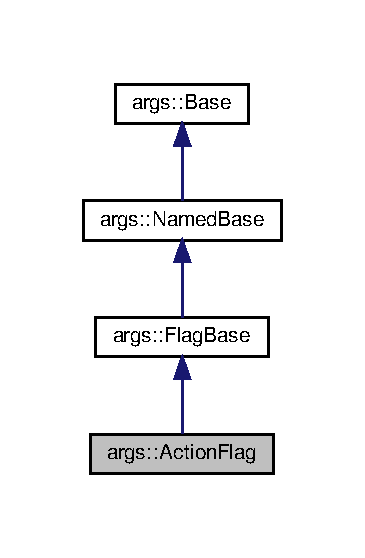
\includegraphics[width=175pt]{classargs_1_1_action_flag__inherit__graph}
\end{center}
\end{figure}


Collaboration diagram for args\+:\+:Action\+Flag\+:\nopagebreak
\begin{figure}[H]
\begin{center}
\leavevmode
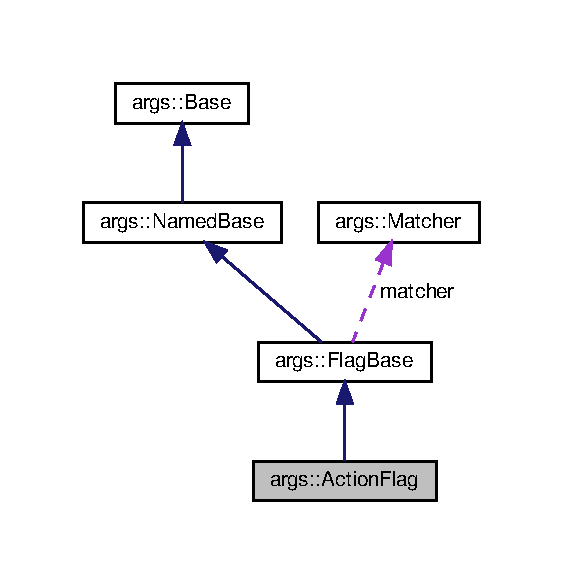
\includegraphics[width=270pt]{classargs_1_1_action_flag__coll__graph}
\end{center}
\end{figure}
\subsection*{Public Member Functions}
\begin{DoxyCompactItemize}
\item 
\hyperlink{classargs_1_1_action_flag_aa0f44a64b894b5cfe2410c9df7addd9d}{Action\+Flag} (\hyperlink{classargs_1_1_group}{Group} \&group\+\_\+, const std\+::string \&name\+\_\+, const std\+::string \&help\+\_\+, \hyperlink{classargs_1_1_matcher}{Matcher} \&\&matcher\+\_\+, \hyperlink{structargs_1_1_nargs}{Nargs} nargs\+\_\+, std\+::function$<$ void(const std\+::vector$<$ std\+::string $>$ \&)$>$ action\+\_\+, \hyperlink{namespaceargs_aa530c0f95194aa275f49a5f299ac9e77}{Options} options\+\_\+=\{\})
\item 
\hyperlink{classargs_1_1_action_flag_a0f5aa72ff82d751962e764e4b71bdff6}{Action\+Flag} (\hyperlink{classargs_1_1_group}{Group} \&group\+\_\+, const std\+::string \&name\+\_\+, const std\+::string \&help\+\_\+, \hyperlink{classargs_1_1_matcher}{Matcher} \&\&matcher\+\_\+, std\+::function$<$ void(const std\+::string \&)$>$ action\+\_\+, \hyperlink{namespaceargs_aa530c0f95194aa275f49a5f299ac9e77}{Options} options\+\_\+=\{\})
\item 
\hyperlink{classargs_1_1_action_flag_a811e7632dface8147a93ac5d19a1bd34}{Action\+Flag} (\hyperlink{classargs_1_1_group}{Group} \&group\+\_\+, const std\+::string \&name\+\_\+, const std\+::string \&help\+\_\+, \hyperlink{classargs_1_1_matcher}{Matcher} \&\&matcher\+\_\+, std\+::function$<$ void()$>$ action\+\_\+, \hyperlink{namespaceargs_aa530c0f95194aa275f49a5f299ac9e77}{Options} options\+\_\+=\{\})
\item 
virtual \hyperlink{structargs_1_1_nargs}{Nargs} \hyperlink{classargs_1_1_action_flag_aa341976acd895df15fb2bfe7182c48eb}{Number\+Of\+Arguments} () const noexcept override
\item 
virtual void \hyperlink{classargs_1_1_action_flag_abffb65449304c0799566c88c90adda0b}{Parse\+Value} (const std\+::vector$<$ std\+::string $>$ \&value) override
\end{DoxyCompactItemize}
\subsection*{Additional Inherited Members}


\subsection{Detailed Description}
A flag class that calls a function when it\textquotesingle{}s matched 

\subsection{Constructor \& Destructor Documentation}
\mbox{\Hypertarget{classargs_1_1_action_flag_aa0f44a64b894b5cfe2410c9df7addd9d}\label{classargs_1_1_action_flag_aa0f44a64b894b5cfe2410c9df7addd9d}} 
\index{args\+::\+Action\+Flag@{args\+::\+Action\+Flag}!Action\+Flag@{Action\+Flag}}
\index{Action\+Flag@{Action\+Flag}!args\+::\+Action\+Flag@{args\+::\+Action\+Flag}}
\subsubsection{\texorpdfstring{Action\+Flag()}{ActionFlag()}\hspace{0.1cm}{\footnotesize\ttfamily [1/3]}}
{\footnotesize\ttfamily args\+::\+Action\+Flag\+::\+Action\+Flag (\begin{DoxyParamCaption}\item[{\hyperlink{classargs_1_1_group}{Group} \&}]{group\+\_\+,  }\item[{const std\+::string \&}]{name\+\_\+,  }\item[{const std\+::string \&}]{help\+\_\+,  }\item[{\hyperlink{classargs_1_1_matcher}{Matcher} \&\&}]{matcher\+\_\+,  }\item[{\hyperlink{structargs_1_1_nargs}{Nargs}}]{nargs\+\_\+,  }\item[{std\+::function$<$ void(const std\+::vector$<$ std\+::string $>$ \&)$>$}]{action\+\_\+,  }\item[{\hyperlink{namespaceargs_aa530c0f95194aa275f49a5f299ac9e77}{Options}}]{options\+\_\+ = {\ttfamily \{\}} }\end{DoxyParamCaption})\hspace{0.3cm}{\ttfamily [inline]}}

\mbox{\Hypertarget{classargs_1_1_action_flag_a0f5aa72ff82d751962e764e4b71bdff6}\label{classargs_1_1_action_flag_a0f5aa72ff82d751962e764e4b71bdff6}} 
\index{args\+::\+Action\+Flag@{args\+::\+Action\+Flag}!Action\+Flag@{Action\+Flag}}
\index{Action\+Flag@{Action\+Flag}!args\+::\+Action\+Flag@{args\+::\+Action\+Flag}}
\subsubsection{\texorpdfstring{Action\+Flag()}{ActionFlag()}\hspace{0.1cm}{\footnotesize\ttfamily [2/3]}}
{\footnotesize\ttfamily args\+::\+Action\+Flag\+::\+Action\+Flag (\begin{DoxyParamCaption}\item[{\hyperlink{classargs_1_1_group}{Group} \&}]{group\+\_\+,  }\item[{const std\+::string \&}]{name\+\_\+,  }\item[{const std\+::string \&}]{help\+\_\+,  }\item[{\hyperlink{classargs_1_1_matcher}{Matcher} \&\&}]{matcher\+\_\+,  }\item[{std\+::function$<$ void(const std\+::string \&)$>$}]{action\+\_\+,  }\item[{\hyperlink{namespaceargs_aa530c0f95194aa275f49a5f299ac9e77}{Options}}]{options\+\_\+ = {\ttfamily \{\}} }\end{DoxyParamCaption})\hspace{0.3cm}{\ttfamily [inline]}}

\mbox{\Hypertarget{classargs_1_1_action_flag_a811e7632dface8147a93ac5d19a1bd34}\label{classargs_1_1_action_flag_a811e7632dface8147a93ac5d19a1bd34}} 
\index{args\+::\+Action\+Flag@{args\+::\+Action\+Flag}!Action\+Flag@{Action\+Flag}}
\index{Action\+Flag@{Action\+Flag}!args\+::\+Action\+Flag@{args\+::\+Action\+Flag}}
\subsubsection{\texorpdfstring{Action\+Flag()}{ActionFlag()}\hspace{0.1cm}{\footnotesize\ttfamily [3/3]}}
{\footnotesize\ttfamily args\+::\+Action\+Flag\+::\+Action\+Flag (\begin{DoxyParamCaption}\item[{\hyperlink{classargs_1_1_group}{Group} \&}]{group\+\_\+,  }\item[{const std\+::string \&}]{name\+\_\+,  }\item[{const std\+::string \&}]{help\+\_\+,  }\item[{\hyperlink{classargs_1_1_matcher}{Matcher} \&\&}]{matcher\+\_\+,  }\item[{std\+::function$<$ void()$>$}]{action\+\_\+,  }\item[{\hyperlink{namespaceargs_aa530c0f95194aa275f49a5f299ac9e77}{Options}}]{options\+\_\+ = {\ttfamily \{\}} }\end{DoxyParamCaption})\hspace{0.3cm}{\ttfamily [inline]}}



\subsection{Member Function Documentation}
\mbox{\Hypertarget{classargs_1_1_action_flag_aa341976acd895df15fb2bfe7182c48eb}\label{classargs_1_1_action_flag_aa341976acd895df15fb2bfe7182c48eb}} 
\index{args\+::\+Action\+Flag@{args\+::\+Action\+Flag}!Number\+Of\+Arguments@{Number\+Of\+Arguments}}
\index{Number\+Of\+Arguments@{Number\+Of\+Arguments}!args\+::\+Action\+Flag@{args\+::\+Action\+Flag}}
\subsubsection{\texorpdfstring{Number\+Of\+Arguments()}{NumberOfArguments()}}
{\footnotesize\ttfamily virtual \hyperlink{structargs_1_1_nargs}{Nargs} args\+::\+Action\+Flag\+::\+Number\+Of\+Arguments (\begin{DoxyParamCaption}{ }\end{DoxyParamCaption}) const\hspace{0.3cm}{\ttfamily [inline]}, {\ttfamily [override]}, {\ttfamily [virtual]}, {\ttfamily [noexcept]}}

Defines how many values can be consumed by this option.

\begin{DoxyReturn}{Returns}
closed interval \mbox{[}min, max\mbox{]} 
\end{DoxyReturn}


Implements \hyperlink{classargs_1_1_flag_base_a6007ffeaa767893cb8eff5333d61673b}{args\+::\+Flag\+Base}.

\mbox{\Hypertarget{classargs_1_1_action_flag_abffb65449304c0799566c88c90adda0b}\label{classargs_1_1_action_flag_abffb65449304c0799566c88c90adda0b}} 
\index{args\+::\+Action\+Flag@{args\+::\+Action\+Flag}!Parse\+Value@{Parse\+Value}}
\index{Parse\+Value@{Parse\+Value}!args\+::\+Action\+Flag@{args\+::\+Action\+Flag}}
\subsubsection{\texorpdfstring{Parse\+Value()}{ParseValue()}}
{\footnotesize\ttfamily virtual void args\+::\+Action\+Flag\+::\+Parse\+Value (\begin{DoxyParamCaption}\item[{const std\+::vector$<$ std\+::string $>$ \&}]{value }\end{DoxyParamCaption})\hspace{0.3cm}{\ttfamily [inline]}, {\ttfamily [override]}, {\ttfamily [virtual]}}

Parse values of this option.


\begin{DoxyParams}{Parameters}
{\em value} & Vector of values. It\textquotesingle{}s size must be in \hyperlink{classargs_1_1_action_flag_aa341976acd895df15fb2bfe7182c48eb}{Number\+Of\+Arguments()} interval. \\
\hline
\end{DoxyParams}


Implements \hyperlink{classargs_1_1_flag_base_a3421d9a595c9426dc73f62604cdee84f}{args\+::\+Flag\+Base}.



The documentation for this class was generated from the following file\+:\begin{DoxyCompactItemize}
\item 
/home/cappelletto/github/self/landing\+\_\+area\+\_\+detector/external/\hyperlink{args_8hxx}{args.\+hxx}\end{DoxyCompactItemize}

\hypertarget{classargs_1_1_argument_parser}{}\section{args\+:\+:Argument\+Parser Class Reference}
\label{classargs_1_1_argument_parser}\index{args\+::\+Argument\+Parser@{args\+::\+Argument\+Parser}}


{\ttfamily \#include $<$args.\+hxx$>$}



Inheritance diagram for args\+:\+:Argument\+Parser\+:\nopagebreak
\begin{figure}[H]
\begin{center}
\leavevmode
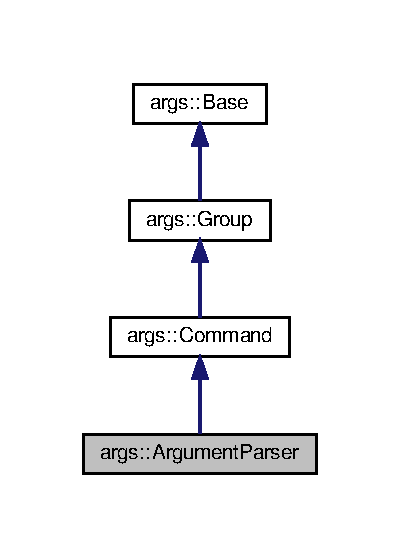
\includegraphics[width=192pt]{classargs_1_1_argument_parser__inherit__graph}
\end{center}
\end{figure}


Collaboration diagram for args\+:\+:Argument\+Parser\+:\nopagebreak
\begin{figure}[H]
\begin{center}
\leavevmode
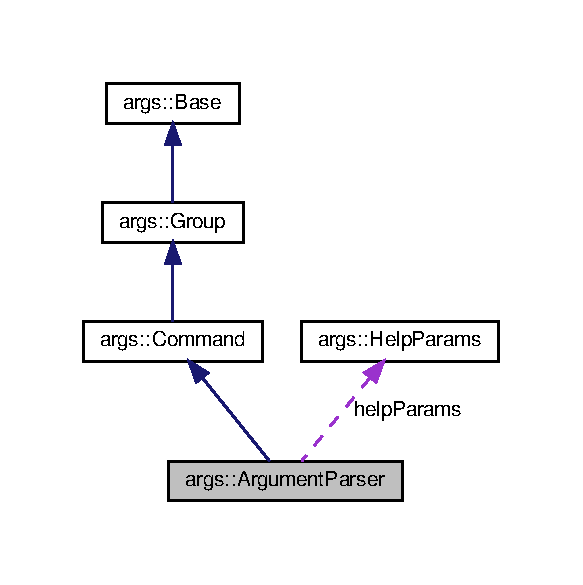
\includegraphics[width=280pt]{classargs_1_1_argument_parser__coll__graph}
\end{center}
\end{figure}
\subsection*{Public Member Functions}
\begin{DoxyCompactItemize}
\item 
\hyperlink{classargs_1_1_argument_parser_a48265b3dc87a042e7c02846dd451b06e}{Argument\+Parser} (const std\+::string \&description\+\_\+, const std\+::string \&epilog\+\_\+=std\+::string())
\item 
const std\+::string \& \hyperlink{classargs_1_1_argument_parser_ac085920cbb59e059fd57233990525707}{Prog} () const
\item 
void \hyperlink{classargs_1_1_argument_parser_a33356eb1ebe72f6f59829237027b17fa}{Prog} (const std\+::string \&prog\+\_\+)
\item 
const std\+::string \& \hyperlink{classargs_1_1_argument_parser_a35f97d0a1219e2a01e10a697b7a24d21}{Long\+Prefix} () const
\item 
void \hyperlink{classargs_1_1_argument_parser_a6a03dcc56b439d54b85e704be5d2f9d5}{Long\+Prefix} (const std\+::string \&longprefix\+\_\+)
\item 
const std\+::string \& \hyperlink{classargs_1_1_argument_parser_afe9cefef0ea866a39fd33815f0f08f92}{Short\+Prefix} () const
\item 
void \hyperlink{classargs_1_1_argument_parser_ad26c7ce7f17994dd0cc81e8137c1e5a8}{Short\+Prefix} (const std\+::string \&shortprefix\+\_\+)
\item 
const std\+::string \& \hyperlink{classargs_1_1_argument_parser_a7bb74e0a1bcac7f390f5bf5a5fef44e6}{Long\+Separator} () const
\item 
void \hyperlink{classargs_1_1_argument_parser_a748cd901c687da9110b52eae1bc1ff74}{Long\+Separator} (const std\+::string \&longseparator\+\_\+)
\item 
const std\+::string \& \hyperlink{classargs_1_1_argument_parser_ae864b7e947bba6c168780b82ebacdb5e}{Terminator} () const
\item 
void \hyperlink{classargs_1_1_argument_parser_aac85423bb4103a71893bc0e0247c1acd}{Terminator} (const std\+::string \&terminator\+\_\+)
\item 
void \hyperlink{classargs_1_1_argument_parser_aba2c63676eeb73db2ea857a03e421513}{Get\+Argument\+Separations} (bool \&allow\+Joined\+Short\+Value\+\_\+, bool \&allow\+Joined\+Long\+Value\+\_\+, bool \&allow\+Separate\+Short\+Value\+\_\+, bool \&allow\+Separate\+Long\+Value\+\_\+) const
\item 
void \hyperlink{classargs_1_1_argument_parser_a067fb46018d370df1629bd9a9d7c0bd0}{Set\+Argument\+Separations} (const bool allow\+Joined\+Short\+Value\+\_\+, const bool allow\+Joined\+Long\+Value\+\_\+, const bool allow\+Separate\+Short\+Value\+\_\+, const bool allow\+Separate\+Long\+Value\+\_\+)
\item 
void \hyperlink{classargs_1_1_argument_parser_a783b7d19d1f2687310adb159418ad234}{Help} (std\+::ostream \&help\+\_\+) const
\item 
std\+::string \hyperlink{classargs_1_1_argument_parser_ac7ca97f929a12508187ed28734ae0714}{Help} () const
\item 
virtual void \hyperlink{classargs_1_1_argument_parser_a73b0dc7bc87c3a44345879f34985237f}{Reset} () noexcept override
\item 
{\footnotesize template$<$typename It $>$ }\\It \hyperlink{classargs_1_1_argument_parser_a4bc1f3f3d000f11715fa66ade894bd9b}{Parse\+Args} (It begin, It end)
\item 
{\footnotesize template$<$typename T $>$ }\\auto \hyperlink{classargs_1_1_argument_parser_aa93289021e58e8ad26f06cd671261c36}{Parse\+Args} (const T \&args) -\/$>$ decltype(std\+::begin(args))
\item 
bool \hyperlink{classargs_1_1_argument_parser_a8e79c5bd015bad9648b9c98eecc63fc9}{Parse\+C\+LI} (const int argc, const char $\ast$const $\ast$argv)
\end{DoxyCompactItemize}
\subsection*{Public Attributes}
\begin{DoxyCompactItemize}
\item 
\hyperlink{structargs_1_1_help_params}{Help\+Params} \hyperlink{classargs_1_1_argument_parser_a0b78172b72e892a6776d2d7dec8e8b46}{help\+Params}
\end{DoxyCompactItemize}
\subsection*{Protected Types}
\begin{DoxyCompactItemize}
\item 
enum \hyperlink{classargs_1_1_argument_parser_af01ec624f521beee7a1ac7ff589a3788}{Option\+Type} \{ \hyperlink{classargs_1_1_argument_parser_af01ec624f521beee7a1ac7ff589a3788a8380e6760c5e0d63b4d457e4fae1e4b9}{Option\+Type\+::\+Long\+Flag}, 
\hyperlink{classargs_1_1_argument_parser_af01ec624f521beee7a1ac7ff589a3788a79741ab7ed4b2321708c779a4fa2ad30}{Option\+Type\+::\+Short\+Flag}, 
\hyperlink{classargs_1_1_argument_parser_af01ec624f521beee7a1ac7ff589a3788ac2c87a0ee60e297b8b4eb1fb26b47bea}{Option\+Type\+::\+Positional}
 \}
\end{DoxyCompactItemize}
\subsection*{Protected Member Functions}
\begin{DoxyCompactItemize}
\item 
\hyperlink{classargs_1_1_argument_parser_af01ec624f521beee7a1ac7ff589a3788}{Option\+Type} \hyperlink{classargs_1_1_argument_parser_a68c6996f0b974924feb1294eb976edf1}{Parse\+Option} (const std\+::string \&s)
\item 
{\footnotesize template$<$typename It $>$ }\\std\+::string \hyperlink{classargs_1_1_argument_parser_ae8ff941317a3df4360c0c8d91f2823bd}{Parse\+Args\+Values} (\hyperlink{classargs_1_1_flag_base}{Flag\+Base} \&flag, const std\+::string \&arg, It \&it, It end, const bool allow\+Separate, const bool allow\+Joined, const bool has\+Joined, const std\+::string \&joined\+Arg, const bool can\+Discard\+Joined, std\+::vector$<$ std\+::string $>$ \&values)
\item 
{\footnotesize template$<$typename It $>$ }\\bool \hyperlink{classargs_1_1_argument_parser_a3143420b4177ce05c076700308d427c2}{Parse\+Long} (It \&it, It end)
\item 
{\footnotesize template$<$typename It $>$ }\\bool \hyperlink{classargs_1_1_argument_parser_a7c975868c3cdcd14465dad5cbaab07b1}{Parse\+Short} (It \&it, It end)
\item 
{\footnotesize template$<$typename It $>$ }\\It \hyperlink{classargs_1_1_argument_parser_a0de11619cf36f34f2e02b787cb92afa6}{Parse} (It begin, It end)
\end{DoxyCompactItemize}
\subsection*{Friends}
\begin{DoxyCompactItemize}
\item 
class \hyperlink{classargs_1_1_argument_parser_aecbd7c0572cb2d7fecb5eff79552c203}{Subparser}
\end{DoxyCompactItemize}
\subsection*{Additional Inherited Members}


\subsection{Detailed Description}
The main user facing command line argument parser class 

\subsection{Member Enumeration Documentation}
\mbox{\Hypertarget{classargs_1_1_argument_parser_af01ec624f521beee7a1ac7ff589a3788}\label{classargs_1_1_argument_parser_af01ec624f521beee7a1ac7ff589a3788}} 
\index{args\+::\+Argument\+Parser@{args\+::\+Argument\+Parser}!Option\+Type@{Option\+Type}}
\index{Option\+Type@{Option\+Type}!args\+::\+Argument\+Parser@{args\+::\+Argument\+Parser}}
\subsubsection{\texorpdfstring{Option\+Type}{OptionType}}
{\footnotesize\ttfamily enum \hyperlink{classargs_1_1_argument_parser_af01ec624f521beee7a1ac7ff589a3788}{args\+::\+Argument\+Parser\+::\+Option\+Type}\hspace{0.3cm}{\ttfamily [strong]}, {\ttfamily [protected]}}

\begin{DoxyEnumFields}{Enumerator}
\raisebox{\heightof{T}}[0pt][0pt]{\index{Long\+Flag@{Long\+Flag}!args\+::\+Argument\+Parser@{args\+::\+Argument\+Parser}}\index{args\+::\+Argument\+Parser@{args\+::\+Argument\+Parser}!Long\+Flag@{Long\+Flag}}}\mbox{\Hypertarget{classargs_1_1_argument_parser_af01ec624f521beee7a1ac7ff589a3788a8380e6760c5e0d63b4d457e4fae1e4b9}\label{classargs_1_1_argument_parser_af01ec624f521beee7a1ac7ff589a3788a8380e6760c5e0d63b4d457e4fae1e4b9}} 
Long\+Flag&\\
\hline

\raisebox{\heightof{T}}[0pt][0pt]{\index{Short\+Flag@{Short\+Flag}!args\+::\+Argument\+Parser@{args\+::\+Argument\+Parser}}\index{args\+::\+Argument\+Parser@{args\+::\+Argument\+Parser}!Short\+Flag@{Short\+Flag}}}\mbox{\Hypertarget{classargs_1_1_argument_parser_af01ec624f521beee7a1ac7ff589a3788a79741ab7ed4b2321708c779a4fa2ad30}\label{classargs_1_1_argument_parser_af01ec624f521beee7a1ac7ff589a3788a79741ab7ed4b2321708c779a4fa2ad30}} 
Short\+Flag&\\
\hline

\raisebox{\heightof{T}}[0pt][0pt]{\index{Positional@{Positional}!args\+::\+Argument\+Parser@{args\+::\+Argument\+Parser}}\index{args\+::\+Argument\+Parser@{args\+::\+Argument\+Parser}!Positional@{Positional}}}\mbox{\Hypertarget{classargs_1_1_argument_parser_af01ec624f521beee7a1ac7ff589a3788ac2c87a0ee60e297b8b4eb1fb26b47bea}\label{classargs_1_1_argument_parser_af01ec624f521beee7a1ac7ff589a3788ac2c87a0ee60e297b8b4eb1fb26b47bea}} 
Positional&\\
\hline

\end{DoxyEnumFields}


\subsection{Constructor \& Destructor Documentation}
\mbox{\Hypertarget{classargs_1_1_argument_parser_a48265b3dc87a042e7c02846dd451b06e}\label{classargs_1_1_argument_parser_a48265b3dc87a042e7c02846dd451b06e}} 
\index{args\+::\+Argument\+Parser@{args\+::\+Argument\+Parser}!Argument\+Parser@{Argument\+Parser}}
\index{Argument\+Parser@{Argument\+Parser}!args\+::\+Argument\+Parser@{args\+::\+Argument\+Parser}}
\subsubsection{\texorpdfstring{Argument\+Parser()}{ArgumentParser()}}
{\footnotesize\ttfamily args\+::\+Argument\+Parser\+::\+Argument\+Parser (\begin{DoxyParamCaption}\item[{const std\+::string \&}]{description\+\_\+,  }\item[{const std\+::string \&}]{epilog\+\_\+ = {\ttfamily std\+:\+:string()} }\end{DoxyParamCaption})\hspace{0.3cm}{\ttfamily [inline]}}



\subsection{Member Function Documentation}
\mbox{\Hypertarget{classargs_1_1_argument_parser_aba2c63676eeb73db2ea857a03e421513}\label{classargs_1_1_argument_parser_aba2c63676eeb73db2ea857a03e421513}} 
\index{args\+::\+Argument\+Parser@{args\+::\+Argument\+Parser}!Get\+Argument\+Separations@{Get\+Argument\+Separations}}
\index{Get\+Argument\+Separations@{Get\+Argument\+Separations}!args\+::\+Argument\+Parser@{args\+::\+Argument\+Parser}}
\subsubsection{\texorpdfstring{Get\+Argument\+Separations()}{GetArgumentSeparations()}}
{\footnotesize\ttfamily void args\+::\+Argument\+Parser\+::\+Get\+Argument\+Separations (\begin{DoxyParamCaption}\item[{bool \&}]{allow\+Joined\+Short\+Value\+\_\+,  }\item[{bool \&}]{allow\+Joined\+Long\+Value\+\_\+,  }\item[{bool \&}]{allow\+Separate\+Short\+Value\+\_\+,  }\item[{bool \&}]{allow\+Separate\+Long\+Value\+\_\+ }\end{DoxyParamCaption}) const\hspace{0.3cm}{\ttfamily [inline]}}

Get the current argument separation parameters.

See Set\+Argument\+Separations for details on what each one means. \mbox{\Hypertarget{classargs_1_1_argument_parser_a783b7d19d1f2687310adb159418ad234}\label{classargs_1_1_argument_parser_a783b7d19d1f2687310adb159418ad234}} 
\index{args\+::\+Argument\+Parser@{args\+::\+Argument\+Parser}!Help@{Help}}
\index{Help@{Help}!args\+::\+Argument\+Parser@{args\+::\+Argument\+Parser}}
\subsubsection{\texorpdfstring{Help()}{Help()}\hspace{0.1cm}{\footnotesize\ttfamily [1/2]}}
{\footnotesize\ttfamily void args\+::\+Argument\+Parser\+::\+Help (\begin{DoxyParamCaption}\item[{std\+::ostream \&}]{help\+\_\+ }\end{DoxyParamCaption}) const\hspace{0.3cm}{\ttfamily [inline]}}

Pass the help menu into an ostream \mbox{\Hypertarget{classargs_1_1_argument_parser_ac7ca97f929a12508187ed28734ae0714}\label{classargs_1_1_argument_parser_ac7ca97f929a12508187ed28734ae0714}} 
\index{args\+::\+Argument\+Parser@{args\+::\+Argument\+Parser}!Help@{Help}}
\index{Help@{Help}!args\+::\+Argument\+Parser@{args\+::\+Argument\+Parser}}
\subsubsection{\texorpdfstring{Help()}{Help()}\hspace{0.1cm}{\footnotesize\ttfamily [2/2]}}
{\footnotesize\ttfamily std\+::string args\+::\+Argument\+Parser\+::\+Help (\begin{DoxyParamCaption}{ }\end{DoxyParamCaption}) const\hspace{0.3cm}{\ttfamily [inline]}}

Generate a help menu as a string.

\begin{DoxyReturn}{Returns}
the help text as a single string 
\end{DoxyReturn}
\mbox{\Hypertarget{classargs_1_1_argument_parser_a35f97d0a1219e2a01e10a697b7a24d21}\label{classargs_1_1_argument_parser_a35f97d0a1219e2a01e10a697b7a24d21}} 
\index{args\+::\+Argument\+Parser@{args\+::\+Argument\+Parser}!Long\+Prefix@{Long\+Prefix}}
\index{Long\+Prefix@{Long\+Prefix}!args\+::\+Argument\+Parser@{args\+::\+Argument\+Parser}}
\subsubsection{\texorpdfstring{Long\+Prefix()}{LongPrefix()}\hspace{0.1cm}{\footnotesize\ttfamily [1/2]}}
{\footnotesize\ttfamily const std\+::string\& args\+::\+Argument\+Parser\+::\+Long\+Prefix (\begin{DoxyParamCaption}{ }\end{DoxyParamCaption}) const\hspace{0.3cm}{\ttfamily [inline]}}

The prefix for long flags \mbox{\Hypertarget{classargs_1_1_argument_parser_a6a03dcc56b439d54b85e704be5d2f9d5}\label{classargs_1_1_argument_parser_a6a03dcc56b439d54b85e704be5d2f9d5}} 
\index{args\+::\+Argument\+Parser@{args\+::\+Argument\+Parser}!Long\+Prefix@{Long\+Prefix}}
\index{Long\+Prefix@{Long\+Prefix}!args\+::\+Argument\+Parser@{args\+::\+Argument\+Parser}}
\subsubsection{\texorpdfstring{Long\+Prefix()}{LongPrefix()}\hspace{0.1cm}{\footnotesize\ttfamily [2/2]}}
{\footnotesize\ttfamily void args\+::\+Argument\+Parser\+::\+Long\+Prefix (\begin{DoxyParamCaption}\item[{const std\+::string \&}]{longprefix\+\_\+ }\end{DoxyParamCaption})\hspace{0.3cm}{\ttfamily [inline]}}

The prefix for long flags \mbox{\Hypertarget{classargs_1_1_argument_parser_a7bb74e0a1bcac7f390f5bf5a5fef44e6}\label{classargs_1_1_argument_parser_a7bb74e0a1bcac7f390f5bf5a5fef44e6}} 
\index{args\+::\+Argument\+Parser@{args\+::\+Argument\+Parser}!Long\+Separator@{Long\+Separator}}
\index{Long\+Separator@{Long\+Separator}!args\+::\+Argument\+Parser@{args\+::\+Argument\+Parser}}
\subsubsection{\texorpdfstring{Long\+Separator()}{LongSeparator()}\hspace{0.1cm}{\footnotesize\ttfamily [1/2]}}
{\footnotesize\ttfamily const std\+::string\& args\+::\+Argument\+Parser\+::\+Long\+Separator (\begin{DoxyParamCaption}{ }\end{DoxyParamCaption}) const\hspace{0.3cm}{\ttfamily [inline]}}

The separator for long flags \mbox{\Hypertarget{classargs_1_1_argument_parser_a748cd901c687da9110b52eae1bc1ff74}\label{classargs_1_1_argument_parser_a748cd901c687da9110b52eae1bc1ff74}} 
\index{args\+::\+Argument\+Parser@{args\+::\+Argument\+Parser}!Long\+Separator@{Long\+Separator}}
\index{Long\+Separator@{Long\+Separator}!args\+::\+Argument\+Parser@{args\+::\+Argument\+Parser}}
\subsubsection{\texorpdfstring{Long\+Separator()}{LongSeparator()}\hspace{0.1cm}{\footnotesize\ttfamily [2/2]}}
{\footnotesize\ttfamily void args\+::\+Argument\+Parser\+::\+Long\+Separator (\begin{DoxyParamCaption}\item[{const std\+::string \&}]{longseparator\+\_\+ }\end{DoxyParamCaption})\hspace{0.3cm}{\ttfamily [inline]}}

The separator for long flags \mbox{\Hypertarget{classargs_1_1_argument_parser_a0de11619cf36f34f2e02b787cb92afa6}\label{classargs_1_1_argument_parser_a0de11619cf36f34f2e02b787cb92afa6}} 
\index{args\+::\+Argument\+Parser@{args\+::\+Argument\+Parser}!Parse@{Parse}}
\index{Parse@{Parse}!args\+::\+Argument\+Parser@{args\+::\+Argument\+Parser}}
\subsubsection{\texorpdfstring{Parse()}{Parse()}}
{\footnotesize\ttfamily template$<$typename It $>$ \\
It args\+::\+Argument\+Parser\+::\+Parse (\begin{DoxyParamCaption}\item[{It}]{begin,  }\item[{It}]{end }\end{DoxyParamCaption})\hspace{0.3cm}{\ttfamily [inline]}, {\ttfamily [protected]}}

\mbox{\Hypertarget{classargs_1_1_argument_parser_a4bc1f3f3d000f11715fa66ade894bd9b}\label{classargs_1_1_argument_parser_a4bc1f3f3d000f11715fa66ade894bd9b}} 
\index{args\+::\+Argument\+Parser@{args\+::\+Argument\+Parser}!Parse\+Args@{Parse\+Args}}
\index{Parse\+Args@{Parse\+Args}!args\+::\+Argument\+Parser@{args\+::\+Argument\+Parser}}
\subsubsection{\texorpdfstring{Parse\+Args()}{ParseArgs()}\hspace{0.1cm}{\footnotesize\ttfamily [1/2]}}
{\footnotesize\ttfamily template$<$typename It $>$ \\
It args\+::\+Argument\+Parser\+::\+Parse\+Args (\begin{DoxyParamCaption}\item[{It}]{begin,  }\item[{It}]{end }\end{DoxyParamCaption})\hspace{0.3cm}{\ttfamily [inline]}}

Parse all arguments.


\begin{DoxyParams}{Parameters}
{\em begin} & an iterator to the beginning of the argument list \\
\hline
{\em end} & an iterator to the past-\/the-\/end element of the argument list \\
\hline
\end{DoxyParams}
\begin{DoxyReturn}{Returns}
the iterator after the last parsed value. Only useful for kick-\/out 
\end{DoxyReturn}
\mbox{\Hypertarget{classargs_1_1_argument_parser_aa93289021e58e8ad26f06cd671261c36}\label{classargs_1_1_argument_parser_aa93289021e58e8ad26f06cd671261c36}} 
\index{args\+::\+Argument\+Parser@{args\+::\+Argument\+Parser}!Parse\+Args@{Parse\+Args}}
\index{Parse\+Args@{Parse\+Args}!args\+::\+Argument\+Parser@{args\+::\+Argument\+Parser}}
\subsubsection{\texorpdfstring{Parse\+Args()}{ParseArgs()}\hspace{0.1cm}{\footnotesize\ttfamily [2/2]}}
{\footnotesize\ttfamily template$<$typename T $>$ \\
auto args\+::\+Argument\+Parser\+::\+Parse\+Args (\begin{DoxyParamCaption}\item[{const T \&}]{args }\end{DoxyParamCaption}) -\/$>$ decltype(std\+::begin(args))
            \hspace{0.3cm}{\ttfamily [inline]}}

Parse all arguments.


\begin{DoxyParams}{Parameters}
{\em args} & an iterable of the arguments \\
\hline
\end{DoxyParams}
\begin{DoxyReturn}{Returns}
the iterator after the last parsed value. Only useful for kick-\/out 
\end{DoxyReturn}
\mbox{\Hypertarget{classargs_1_1_argument_parser_ae8ff941317a3df4360c0c8d91f2823bd}\label{classargs_1_1_argument_parser_ae8ff941317a3df4360c0c8d91f2823bd}} 
\index{args\+::\+Argument\+Parser@{args\+::\+Argument\+Parser}!Parse\+Args\+Values@{Parse\+Args\+Values}}
\index{Parse\+Args\+Values@{Parse\+Args\+Values}!args\+::\+Argument\+Parser@{args\+::\+Argument\+Parser}}
\subsubsection{\texorpdfstring{Parse\+Args\+Values()}{ParseArgsValues()}}
{\footnotesize\ttfamily template$<$typename It $>$ \\
std\+::string args\+::\+Argument\+Parser\+::\+Parse\+Args\+Values (\begin{DoxyParamCaption}\item[{\hyperlink{classargs_1_1_flag_base}{Flag\+Base} \&}]{flag,  }\item[{const std\+::string \&}]{arg,  }\item[{It \&}]{it,  }\item[{It}]{end,  }\item[{const bool}]{allow\+Separate,  }\item[{const bool}]{allow\+Joined,  }\item[{const bool}]{has\+Joined,  }\item[{const std\+::string \&}]{joined\+Arg,  }\item[{const bool}]{can\+Discard\+Joined,  }\item[{std\+::vector$<$ std\+::string $>$ \&}]{values }\end{DoxyParamCaption})\hspace{0.3cm}{\ttfamily [inline]}, {\ttfamily [protected]}}

(I\+N\+T\+E\+R\+N\+AL) Parse flag\textquotesingle{}s values


\begin{DoxyParams}[1]{Parameters}
 & {\em arg} & The string to display in error message as a flag name \\
\hline
\mbox{\tt in,out}  & {\em it} & The iterator to first value. It will point to the last value \\
\hline
 & {\em end} & The end iterator \\
\hline
 & {\em joined\+Arg} & Joined value (e.\+g. bar in --foo=bar) \\
\hline
 & {\em can\+Discard\+Joined} & If true joined value can be parsed as flag not as a value (as in -\/abcd) \\
\hline
\mbox{\tt out}  & {\em values} & The vector to store parsed arg\textquotesingle{}s values \\
\hline
\end{DoxyParams}
\mbox{\Hypertarget{classargs_1_1_argument_parser_a8e79c5bd015bad9648b9c98eecc63fc9}\label{classargs_1_1_argument_parser_a8e79c5bd015bad9648b9c98eecc63fc9}} 
\index{args\+::\+Argument\+Parser@{args\+::\+Argument\+Parser}!Parse\+C\+LI@{Parse\+C\+LI}}
\index{Parse\+C\+LI@{Parse\+C\+LI}!args\+::\+Argument\+Parser@{args\+::\+Argument\+Parser}}
\subsubsection{\texorpdfstring{Parse\+C\+L\+I()}{ParseCLI()}}
{\footnotesize\ttfamily bool args\+::\+Argument\+Parser\+::\+Parse\+C\+LI (\begin{DoxyParamCaption}\item[{const int}]{argc,  }\item[{const char $\ast$const $\ast$}]{argv }\end{DoxyParamCaption})\hspace{0.3cm}{\ttfamily [inline]}}

Convenience function to parse the C\+LI from argc and argv

Just assigns the program name and vectorizes arguments for passing into \hyperlink{classargs_1_1_argument_parser_a4bc1f3f3d000f11715fa66ade894bd9b}{Parse\+Args()}

\begin{DoxyReturn}{Returns}
whether or not all arguments were parsed. This works for detecting kick-\/out, but is generally useless as it can\textquotesingle{}t do anything with it. 
\end{DoxyReturn}
\mbox{\Hypertarget{classargs_1_1_argument_parser_a3143420b4177ce05c076700308d427c2}\label{classargs_1_1_argument_parser_a3143420b4177ce05c076700308d427c2}} 
\index{args\+::\+Argument\+Parser@{args\+::\+Argument\+Parser}!Parse\+Long@{Parse\+Long}}
\index{Parse\+Long@{Parse\+Long}!args\+::\+Argument\+Parser@{args\+::\+Argument\+Parser}}
\subsubsection{\texorpdfstring{Parse\+Long()}{ParseLong()}}
{\footnotesize\ttfamily template$<$typename It $>$ \\
bool args\+::\+Argument\+Parser\+::\+Parse\+Long (\begin{DoxyParamCaption}\item[{It \&}]{it,  }\item[{It}]{end }\end{DoxyParamCaption})\hspace{0.3cm}{\ttfamily [inline]}, {\ttfamily [protected]}}

\mbox{\Hypertarget{classargs_1_1_argument_parser_a68c6996f0b974924feb1294eb976edf1}\label{classargs_1_1_argument_parser_a68c6996f0b974924feb1294eb976edf1}} 
\index{args\+::\+Argument\+Parser@{args\+::\+Argument\+Parser}!Parse\+Option@{Parse\+Option}}
\index{Parse\+Option@{Parse\+Option}!args\+::\+Argument\+Parser@{args\+::\+Argument\+Parser}}
\subsubsection{\texorpdfstring{Parse\+Option()}{ParseOption()}}
{\footnotesize\ttfamily \hyperlink{classargs_1_1_argument_parser_af01ec624f521beee7a1ac7ff589a3788}{Option\+Type} args\+::\+Argument\+Parser\+::\+Parse\+Option (\begin{DoxyParamCaption}\item[{const std\+::string \&}]{s }\end{DoxyParamCaption})\hspace{0.3cm}{\ttfamily [inline]}, {\ttfamily [protected]}}

\mbox{\Hypertarget{classargs_1_1_argument_parser_a7c975868c3cdcd14465dad5cbaab07b1}\label{classargs_1_1_argument_parser_a7c975868c3cdcd14465dad5cbaab07b1}} 
\index{args\+::\+Argument\+Parser@{args\+::\+Argument\+Parser}!Parse\+Short@{Parse\+Short}}
\index{Parse\+Short@{Parse\+Short}!args\+::\+Argument\+Parser@{args\+::\+Argument\+Parser}}
\subsubsection{\texorpdfstring{Parse\+Short()}{ParseShort()}}
{\footnotesize\ttfamily template$<$typename It $>$ \\
bool args\+::\+Argument\+Parser\+::\+Parse\+Short (\begin{DoxyParamCaption}\item[{It \&}]{it,  }\item[{It}]{end }\end{DoxyParamCaption})\hspace{0.3cm}{\ttfamily [inline]}, {\ttfamily [protected]}}

\mbox{\Hypertarget{classargs_1_1_argument_parser_ac085920cbb59e059fd57233990525707}\label{classargs_1_1_argument_parser_ac085920cbb59e059fd57233990525707}} 
\index{args\+::\+Argument\+Parser@{args\+::\+Argument\+Parser}!Prog@{Prog}}
\index{Prog@{Prog}!args\+::\+Argument\+Parser@{args\+::\+Argument\+Parser}}
\subsubsection{\texorpdfstring{Prog()}{Prog()}\hspace{0.1cm}{\footnotesize\ttfamily [1/2]}}
{\footnotesize\ttfamily const std\+::string\& args\+::\+Argument\+Parser\+::\+Prog (\begin{DoxyParamCaption}{ }\end{DoxyParamCaption}) const\hspace{0.3cm}{\ttfamily [inline]}}

The program name for help generation \mbox{\Hypertarget{classargs_1_1_argument_parser_a33356eb1ebe72f6f59829237027b17fa}\label{classargs_1_1_argument_parser_a33356eb1ebe72f6f59829237027b17fa}} 
\index{args\+::\+Argument\+Parser@{args\+::\+Argument\+Parser}!Prog@{Prog}}
\index{Prog@{Prog}!args\+::\+Argument\+Parser@{args\+::\+Argument\+Parser}}
\subsubsection{\texorpdfstring{Prog()}{Prog()}\hspace{0.1cm}{\footnotesize\ttfamily [2/2]}}
{\footnotesize\ttfamily void args\+::\+Argument\+Parser\+::\+Prog (\begin{DoxyParamCaption}\item[{const std\+::string \&}]{prog\+\_\+ }\end{DoxyParamCaption})\hspace{0.3cm}{\ttfamily [inline]}}

The program name for help generation \mbox{\Hypertarget{classargs_1_1_argument_parser_a73b0dc7bc87c3a44345879f34985237f}\label{classargs_1_1_argument_parser_a73b0dc7bc87c3a44345879f34985237f}} 
\index{args\+::\+Argument\+Parser@{args\+::\+Argument\+Parser}!Reset@{Reset}}
\index{Reset@{Reset}!args\+::\+Argument\+Parser@{args\+::\+Argument\+Parser}}
\subsubsection{\texorpdfstring{Reset()}{Reset()}}
{\footnotesize\ttfamily virtual void args\+::\+Argument\+Parser\+::\+Reset (\begin{DoxyParamCaption}{ }\end{DoxyParamCaption})\hspace{0.3cm}{\ttfamily [inline]}, {\ttfamily [override]}, {\ttfamily [virtual]}, {\ttfamily [noexcept]}}



Reimplemented from \hyperlink{classargs_1_1_command_aa1829501dd4f63ba3551bf85171be83e}{args\+::\+Command}.

\mbox{\Hypertarget{classargs_1_1_argument_parser_a067fb46018d370df1629bd9a9d7c0bd0}\label{classargs_1_1_argument_parser_a067fb46018d370df1629bd9a9d7c0bd0}} 
\index{args\+::\+Argument\+Parser@{args\+::\+Argument\+Parser}!Set\+Argument\+Separations@{Set\+Argument\+Separations}}
\index{Set\+Argument\+Separations@{Set\+Argument\+Separations}!args\+::\+Argument\+Parser@{args\+::\+Argument\+Parser}}
\subsubsection{\texorpdfstring{Set\+Argument\+Separations()}{SetArgumentSeparations()}}
{\footnotesize\ttfamily void args\+::\+Argument\+Parser\+::\+Set\+Argument\+Separations (\begin{DoxyParamCaption}\item[{const bool}]{allow\+Joined\+Short\+Value\+\_\+,  }\item[{const bool}]{allow\+Joined\+Long\+Value\+\_\+,  }\item[{const bool}]{allow\+Separate\+Short\+Value\+\_\+,  }\item[{const bool}]{allow\+Separate\+Long\+Value\+\_\+ }\end{DoxyParamCaption})\hspace{0.3cm}{\ttfamily [inline]}}

Change allowed option separation.


\begin{DoxyParams}{Parameters}
{\em allow\+Joined\+Short\+Value\+\_\+} & Allow a short flag that accepts an argument to be passed its argument immediately next to it (ie. in the same argv field) \\
\hline
{\em allow\+Joined\+Long\+Value\+\_\+} & Allow a long flag that accepts an argument to be passed its argument separated by the longseparator (ie. in the same argv field) \\
\hline
{\em allow\+Separate\+Short\+Value\+\_\+} & Allow a short flag that accepts an argument to be passed its argument separated by whitespace (ie. in the next argv field) \\
\hline
{\em allow\+Separate\+Long\+Value\+\_\+} & Allow a long flag that accepts an argument to be passed its argument separated by whitespace (ie. in the next argv field) \\
\hline
\end{DoxyParams}
\mbox{\Hypertarget{classargs_1_1_argument_parser_afe9cefef0ea866a39fd33815f0f08f92}\label{classargs_1_1_argument_parser_afe9cefef0ea866a39fd33815f0f08f92}} 
\index{args\+::\+Argument\+Parser@{args\+::\+Argument\+Parser}!Short\+Prefix@{Short\+Prefix}}
\index{Short\+Prefix@{Short\+Prefix}!args\+::\+Argument\+Parser@{args\+::\+Argument\+Parser}}
\subsubsection{\texorpdfstring{Short\+Prefix()}{ShortPrefix()}\hspace{0.1cm}{\footnotesize\ttfamily [1/2]}}
{\footnotesize\ttfamily const std\+::string\& args\+::\+Argument\+Parser\+::\+Short\+Prefix (\begin{DoxyParamCaption}{ }\end{DoxyParamCaption}) const\hspace{0.3cm}{\ttfamily [inline]}}

The prefix for short flags \mbox{\Hypertarget{classargs_1_1_argument_parser_ad26c7ce7f17994dd0cc81e8137c1e5a8}\label{classargs_1_1_argument_parser_ad26c7ce7f17994dd0cc81e8137c1e5a8}} 
\index{args\+::\+Argument\+Parser@{args\+::\+Argument\+Parser}!Short\+Prefix@{Short\+Prefix}}
\index{Short\+Prefix@{Short\+Prefix}!args\+::\+Argument\+Parser@{args\+::\+Argument\+Parser}}
\subsubsection{\texorpdfstring{Short\+Prefix()}{ShortPrefix()}\hspace{0.1cm}{\footnotesize\ttfamily [2/2]}}
{\footnotesize\ttfamily void args\+::\+Argument\+Parser\+::\+Short\+Prefix (\begin{DoxyParamCaption}\item[{const std\+::string \&}]{shortprefix\+\_\+ }\end{DoxyParamCaption})\hspace{0.3cm}{\ttfamily [inline]}}

The prefix for short flags \mbox{\Hypertarget{classargs_1_1_argument_parser_ae864b7e947bba6c168780b82ebacdb5e}\label{classargs_1_1_argument_parser_ae864b7e947bba6c168780b82ebacdb5e}} 
\index{args\+::\+Argument\+Parser@{args\+::\+Argument\+Parser}!Terminator@{Terminator}}
\index{Terminator@{Terminator}!args\+::\+Argument\+Parser@{args\+::\+Argument\+Parser}}
\subsubsection{\texorpdfstring{Terminator()}{Terminator()}\hspace{0.1cm}{\footnotesize\ttfamily [1/2]}}
{\footnotesize\ttfamily const std\+::string\& args\+::\+Argument\+Parser\+::\+Terminator (\begin{DoxyParamCaption}{ }\end{DoxyParamCaption}) const\hspace{0.3cm}{\ttfamily [inline]}}

The terminator that forcibly separates flags from positionals \mbox{\Hypertarget{classargs_1_1_argument_parser_aac85423bb4103a71893bc0e0247c1acd}\label{classargs_1_1_argument_parser_aac85423bb4103a71893bc0e0247c1acd}} 
\index{args\+::\+Argument\+Parser@{args\+::\+Argument\+Parser}!Terminator@{Terminator}}
\index{Terminator@{Terminator}!args\+::\+Argument\+Parser@{args\+::\+Argument\+Parser}}
\subsubsection{\texorpdfstring{Terminator()}{Terminator()}\hspace{0.1cm}{\footnotesize\ttfamily [2/2]}}
{\footnotesize\ttfamily void args\+::\+Argument\+Parser\+::\+Terminator (\begin{DoxyParamCaption}\item[{const std\+::string \&}]{terminator\+\_\+ }\end{DoxyParamCaption})\hspace{0.3cm}{\ttfamily [inline]}}

The terminator that forcibly separates flags from positionals 

\subsection{Friends And Related Function Documentation}
\mbox{\Hypertarget{classargs_1_1_argument_parser_aecbd7c0572cb2d7fecb5eff79552c203}\label{classargs_1_1_argument_parser_aecbd7c0572cb2d7fecb5eff79552c203}} 
\index{args\+::\+Argument\+Parser@{args\+::\+Argument\+Parser}!Subparser@{Subparser}}
\index{Subparser@{Subparser}!args\+::\+Argument\+Parser@{args\+::\+Argument\+Parser}}
\subsubsection{\texorpdfstring{Subparser}{Subparser}}
{\footnotesize\ttfamily friend class \hyperlink{classargs_1_1_subparser}{Subparser}\hspace{0.3cm}{\ttfamily [friend]}}



\subsection{Member Data Documentation}
\mbox{\Hypertarget{classargs_1_1_argument_parser_a0b78172b72e892a6776d2d7dec8e8b46}\label{classargs_1_1_argument_parser_a0b78172b72e892a6776d2d7dec8e8b46}} 
\index{args\+::\+Argument\+Parser@{args\+::\+Argument\+Parser}!help\+Params@{help\+Params}}
\index{help\+Params@{help\+Params}!args\+::\+Argument\+Parser@{args\+::\+Argument\+Parser}}
\subsubsection{\texorpdfstring{help\+Params}{helpParams}}
{\footnotesize\ttfamily \hyperlink{structargs_1_1_help_params}{Help\+Params} args\+::\+Argument\+Parser\+::help\+Params}



The documentation for this class was generated from the following file\+:\begin{DoxyCompactItemize}
\item 
/home/cappelletto/github/self/landing\+\_\+area\+\_\+detector/external/\hyperlink{args_8hxx}{args.\+hxx}\end{DoxyCompactItemize}

\hypertarget{classargs_1_1_base}{}\section{args\+:\+:Base Class Reference}
\label{classargs_1_1_base}\index{args\+::\+Base@{args\+::\+Base}}


{\ttfamily \#include $<$args.\+hxx$>$}



Inheritance diagram for args\+:\+:Base\+:\nopagebreak
\begin{figure}[H]
\begin{center}
\leavevmode
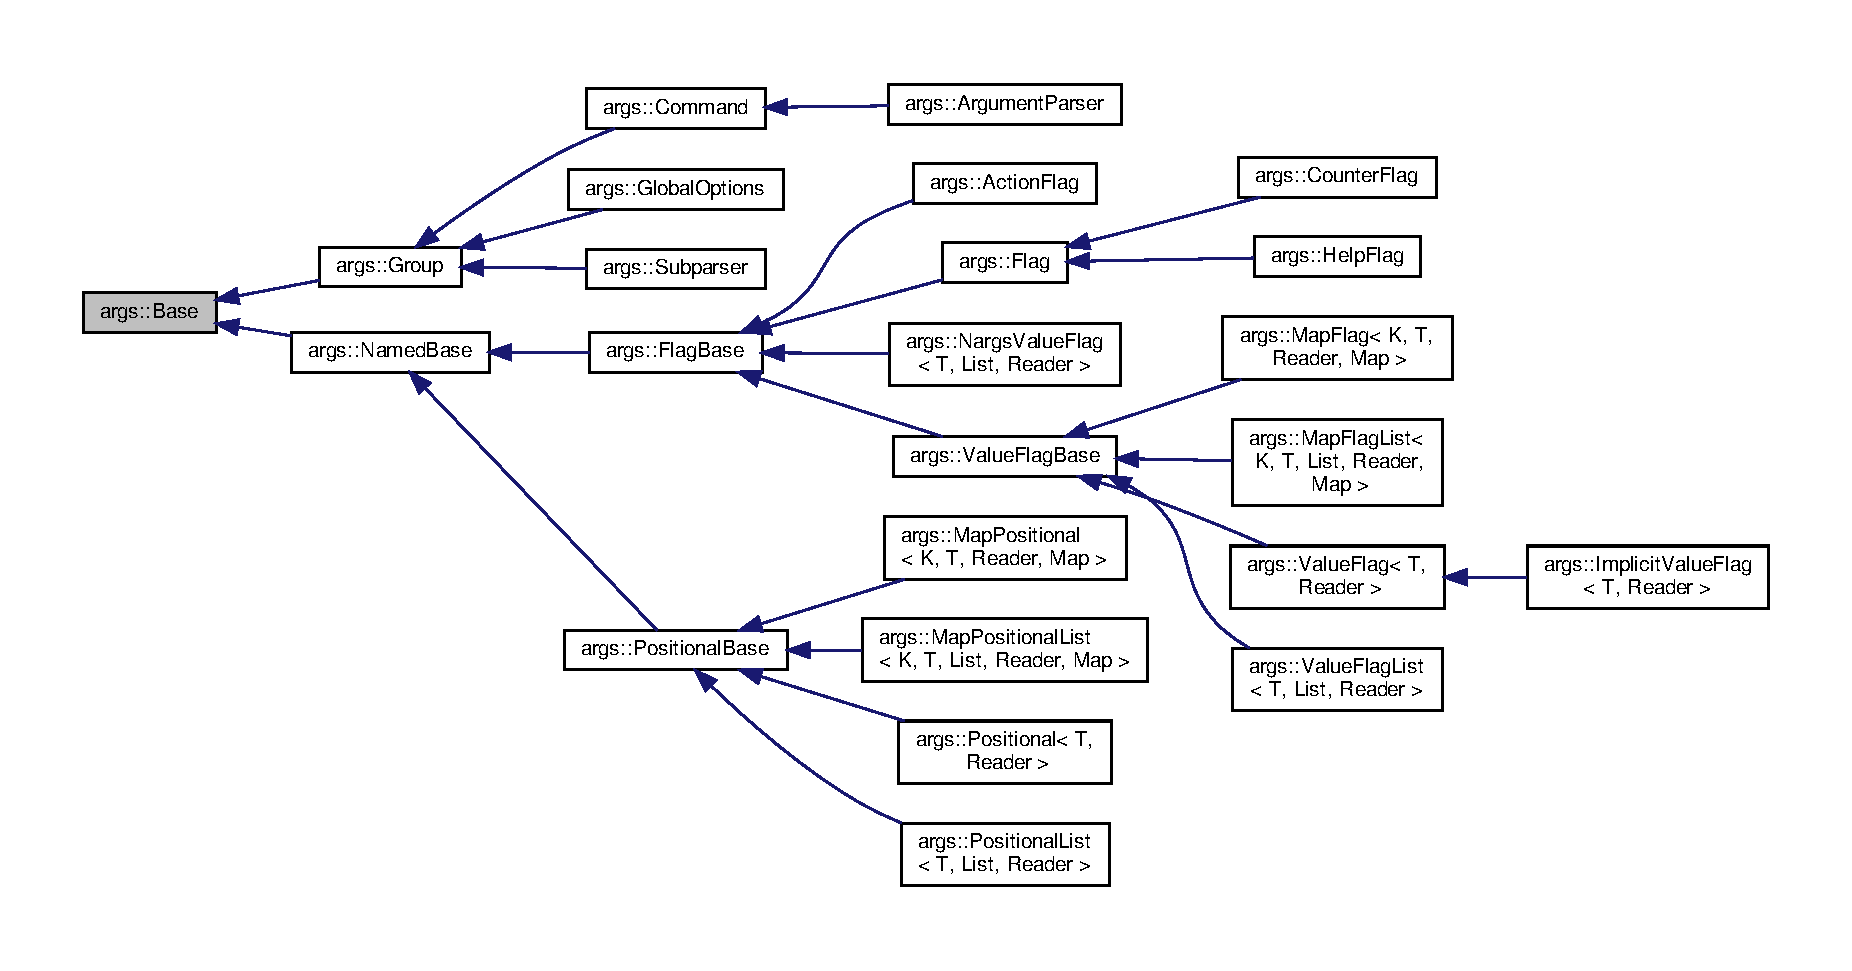
\includegraphics[width=350pt]{classargs_1_1_base__inherit__graph}
\end{center}
\end{figure}
\subsection*{Public Member Functions}
\begin{DoxyCompactItemize}
\item 
\hyperlink{classargs_1_1_base_a70f9c2513df7df1dcf6cab427bb77dce}{Base} (const std\+::string \&help\+\_\+, \hyperlink{namespaceargs_aa530c0f95194aa275f49a5f299ac9e77}{Options} options\+\_\+=\{\})
\item 
virtual \hyperlink{classargs_1_1_base_a30b61d4bac37578b989df06713781de9}{$\sim$\+Base} ()
\item 
\hyperlink{namespaceargs_aa530c0f95194aa275f49a5f299ac9e77}{Options} \hyperlink{classargs_1_1_base_ad44e55adfb22e0ddb0ac5e4248614143}{Get\+Options} () const noexcept
\item 
bool \hyperlink{classargs_1_1_base_a3d705fcb8aa72e6f16a18e47dee12a62}{Is\+Required} () const noexcept
\item 
virtual bool \hyperlink{classargs_1_1_base_ae7ae4ca8ad953be1a353991c1df6ec4d}{Matched} () const noexcept
\item 
virtual void \hyperlink{classargs_1_1_base_a62ea917978306062785cbfaa4dd51d2f}{Validate} (const std\+::string \&, const std\+::string \&) const
\item 
\hyperlink{classargs_1_1_base_ad356e2bd5711e86d005bdc7c483a347e}{operator bool} () const noexcept
\item 
virtual std\+::vector$<$ std\+::tuple$<$ std\+::string, std\+::string, unsigned $>$ $>$ \hyperlink{classargs_1_1_base_afbdf4f1ca1f61182ef0461e02e9e9ed3}{Get\+Description} (const \hyperlink{structargs_1_1_help_params}{Help\+Params} \&, const unsigned indent\+Level) const
\item 
virtual std\+::vector$<$ \hyperlink{classargs_1_1_command}{Command} $\ast$ $>$ \hyperlink{classargs_1_1_base_a8b41df1247be5545f95279608d835bf2}{Get\+Commands} ()
\item 
virtual bool \hyperlink{classargs_1_1_base_a72e11d38c82b8dca87b830853676b68c}{Is\+Group} () const
\item 
virtual \hyperlink{classargs_1_1_flag_base}{Flag\+Base} $\ast$ \hyperlink{classargs_1_1_base_a6d5a7be35d62f59fee5a52c06af3003e}{Match} (const \hyperlink{structargs_1_1_either_flag}{Either\+Flag} \&)
\item 
virtual \hyperlink{classargs_1_1_positional_base}{Positional\+Base} $\ast$ \hyperlink{classargs_1_1_base_a3e5ad8516fd2037496cd39bcb3b10f9d}{Get\+Next\+Positional} ()
\item 
virtual bool \hyperlink{classargs_1_1_base_a81684f399665c0372439c070af5de4a7}{Has\+Flag} () const
\item 
virtual bool \hyperlink{classargs_1_1_base_a3825f4afe867335438103a0d45ced9f7}{Has\+Positional} () const
\item 
virtual bool \hyperlink{classargs_1_1_base_a78322109f31edba4bb467d73e6663422}{Has\+Command} () const
\item 
virtual std\+::vector$<$ std\+::string $>$ \hyperlink{classargs_1_1_base_a88fcbbc4bfe3b7af9fafe6e96a19f337}{Get\+Program\+Line} (const \hyperlink{structargs_1_1_help_params}{Help\+Params} \&) const
\item 
void \hyperlink{classargs_1_1_base_a2a1d655c5d36c58fd19ca30d927d85b8}{Kick\+Out} (bool kickout\+\_\+) noexcept
\begin{DoxyCompactList}\small\item\em Sets a kick-\/out value for building subparsers. \end{DoxyCompactList}\item 
bool \hyperlink{classargs_1_1_base_a83a630e1e05295ab6d2610d2a68082b6}{Kick\+Out} () const noexcept
\begin{DoxyCompactList}\small\item\em Gets the kick-\/out value for building subparsers. \end{DoxyCompactList}\item 
virtual void \hyperlink{classargs_1_1_base_ac7cfc851174f71e00173121d3013dab1}{Reset} () noexcept
\end{DoxyCompactItemize}
\subsection*{Protected Attributes}
\begin{DoxyCompactItemize}
\item 
bool \hyperlink{classargs_1_1_base_a8af1b95de08c309b60c3784a70b65bf1}{matched} = false
\item 
const std\+::string \hyperlink{classargs_1_1_base_a9cdbbcdfa8e764c25f94dfe2c99c3b24}{help}
\end{DoxyCompactItemize}


\subsection{Detailed Description}
\hyperlink{classargs_1_1_base}{Base} class for all match types 

\subsection{Constructor \& Destructor Documentation}
\mbox{\Hypertarget{classargs_1_1_base_a70f9c2513df7df1dcf6cab427bb77dce}\label{classargs_1_1_base_a70f9c2513df7df1dcf6cab427bb77dce}} 
\index{args\+::\+Base@{args\+::\+Base}!Base@{Base}}
\index{Base@{Base}!args\+::\+Base@{args\+::\+Base}}
\subsubsection{\texorpdfstring{Base()}{Base()}}
{\footnotesize\ttfamily args\+::\+Base\+::\+Base (\begin{DoxyParamCaption}\item[{const std\+::string \&}]{help\+\_\+,  }\item[{\hyperlink{namespaceargs_aa530c0f95194aa275f49a5f299ac9e77}{Options}}]{options\+\_\+ = {\ttfamily \{\}} }\end{DoxyParamCaption})\hspace{0.3cm}{\ttfamily [inline]}}

\mbox{\Hypertarget{classargs_1_1_base_a30b61d4bac37578b989df06713781de9}\label{classargs_1_1_base_a30b61d4bac37578b989df06713781de9}} 
\index{args\+::\+Base@{args\+::\+Base}!````~Base@{$\sim$\+Base}}
\index{````~Base@{$\sim$\+Base}!args\+::\+Base@{args\+::\+Base}}
\subsubsection{\texorpdfstring{$\sim$\+Base()}{~Base()}}
{\footnotesize\ttfamily virtual args\+::\+Base\+::$\sim$\+Base (\begin{DoxyParamCaption}{ }\end{DoxyParamCaption})\hspace{0.3cm}{\ttfamily [inline]}, {\ttfamily [virtual]}}



\subsection{Member Function Documentation}
\mbox{\Hypertarget{classargs_1_1_base_a8b41df1247be5545f95279608d835bf2}\label{classargs_1_1_base_a8b41df1247be5545f95279608d835bf2}} 
\index{args\+::\+Base@{args\+::\+Base}!Get\+Commands@{Get\+Commands}}
\index{Get\+Commands@{Get\+Commands}!args\+::\+Base@{args\+::\+Base}}
\subsubsection{\texorpdfstring{Get\+Commands()}{GetCommands()}}
{\footnotesize\ttfamily virtual std\+::vector$<$\hyperlink{classargs_1_1_command}{Command}$\ast$$>$ args\+::\+Base\+::\+Get\+Commands (\begin{DoxyParamCaption}{ }\end{DoxyParamCaption})\hspace{0.3cm}{\ttfamily [inline]}, {\ttfamily [virtual]}}



Reimplemented in \hyperlink{classargs_1_1_command_a59511be164aa3a0cc5fbbfb75ca79fec}{args\+::\+Command}, and \hyperlink{classargs_1_1_group_a83b0a40e16d92c0f387d00a0f35dbf17}{args\+::\+Group}.

\mbox{\Hypertarget{classargs_1_1_base_afbdf4f1ca1f61182ef0461e02e9e9ed3}\label{classargs_1_1_base_afbdf4f1ca1f61182ef0461e02e9e9ed3}} 
\index{args\+::\+Base@{args\+::\+Base}!Get\+Description@{Get\+Description}}
\index{Get\+Description@{Get\+Description}!args\+::\+Base@{args\+::\+Base}}
\subsubsection{\texorpdfstring{Get\+Description()}{GetDescription()}}
{\footnotesize\ttfamily virtual std\+::vector$<$std\+::tuple$<$std\+::string, std\+::string, unsigned$>$ $>$ args\+::\+Base\+::\+Get\+Description (\begin{DoxyParamCaption}\item[{const \hyperlink{structargs_1_1_help_params}{Help\+Params} \&}]{,  }\item[{const unsigned}]{indent\+Level }\end{DoxyParamCaption}) const\hspace{0.3cm}{\ttfamily [inline]}, {\ttfamily [virtual]}}



Reimplemented in \hyperlink{classargs_1_1_named_base_ab0b9e1f22abf04b24659fada61a6d665}{args\+::\+Named\+Base}.

\mbox{\Hypertarget{classargs_1_1_base_a3e5ad8516fd2037496cd39bcb3b10f9d}\label{classargs_1_1_base_a3e5ad8516fd2037496cd39bcb3b10f9d}} 
\index{args\+::\+Base@{args\+::\+Base}!Get\+Next\+Positional@{Get\+Next\+Positional}}
\index{Get\+Next\+Positional@{Get\+Next\+Positional}!args\+::\+Base@{args\+::\+Base}}
\subsubsection{\texorpdfstring{Get\+Next\+Positional()}{GetNextPositional()}}
{\footnotesize\ttfamily virtual \hyperlink{classargs_1_1_positional_base}{Positional\+Base}$\ast$ args\+::\+Base\+::\+Get\+Next\+Positional (\begin{DoxyParamCaption}{ }\end{DoxyParamCaption})\hspace{0.3cm}{\ttfamily [inline]}, {\ttfamily [virtual]}}



Reimplemented in \hyperlink{classargs_1_1_command_a073266d188b3592f745c64567e566f8a}{args\+::\+Command}, \hyperlink{classargs_1_1_group_ae0fa8f5ae77fda45086e7815617ddff7}{args\+::\+Group}, and \hyperlink{classargs_1_1_positional_base_aaaf09006fd551306b979ea026c49bddb}{args\+::\+Positional\+Base}.

\mbox{\Hypertarget{classargs_1_1_base_ad44e55adfb22e0ddb0ac5e4248614143}\label{classargs_1_1_base_ad44e55adfb22e0ddb0ac5e4248614143}} 
\index{args\+::\+Base@{args\+::\+Base}!Get\+Options@{Get\+Options}}
\index{Get\+Options@{Get\+Options}!args\+::\+Base@{args\+::\+Base}}
\subsubsection{\texorpdfstring{Get\+Options()}{GetOptions()}}
{\footnotesize\ttfamily \hyperlink{namespaceargs_aa530c0f95194aa275f49a5f299ac9e77}{Options} args\+::\+Base\+::\+Get\+Options (\begin{DoxyParamCaption}{ }\end{DoxyParamCaption}) const\hspace{0.3cm}{\ttfamily [inline]}, {\ttfamily [noexcept]}}

\mbox{\Hypertarget{classargs_1_1_base_a88fcbbc4bfe3b7af9fafe6e96a19f337}\label{classargs_1_1_base_a88fcbbc4bfe3b7af9fafe6e96a19f337}} 
\index{args\+::\+Base@{args\+::\+Base}!Get\+Program\+Line@{Get\+Program\+Line}}
\index{Get\+Program\+Line@{Get\+Program\+Line}!args\+::\+Base@{args\+::\+Base}}
\subsubsection{\texorpdfstring{Get\+Program\+Line()}{GetProgramLine()}}
{\footnotesize\ttfamily virtual std\+::vector$<$std\+::string$>$ args\+::\+Base\+::\+Get\+Program\+Line (\begin{DoxyParamCaption}\item[{const \hyperlink{structargs_1_1_help_params}{Help\+Params} \&}]{ }\end{DoxyParamCaption}) const\hspace{0.3cm}{\ttfamily [inline]}, {\ttfamily [virtual]}}



Reimplemented in \hyperlink{classargs_1_1_command_a37fbbde216ce232279e04edce12c1245}{args\+::\+Command}, \hyperlink{classargs_1_1_group_abe9ab07499ec19e941df8f38e18089df}{args\+::\+Group}, \hyperlink{classargs_1_1_positional_base_a5bf0bc66f4b8cc5aa414fe8976ab8129}{args\+::\+Positional\+Base}, and \hyperlink{classargs_1_1_flag_base_aeb3153e728d38f0f3e0ea5df46fb4acc}{args\+::\+Flag\+Base}.

\mbox{\Hypertarget{classargs_1_1_base_a78322109f31edba4bb467d73e6663422}\label{classargs_1_1_base_a78322109f31edba4bb467d73e6663422}} 
\index{args\+::\+Base@{args\+::\+Base}!Has\+Command@{Has\+Command}}
\index{Has\+Command@{Has\+Command}!args\+::\+Base@{args\+::\+Base}}
\subsubsection{\texorpdfstring{Has\+Command()}{HasCommand()}}
{\footnotesize\ttfamily virtual bool args\+::\+Base\+::\+Has\+Command (\begin{DoxyParamCaption}{ }\end{DoxyParamCaption}) const\hspace{0.3cm}{\ttfamily [inline]}, {\ttfamily [virtual]}}



Reimplemented in \hyperlink{classargs_1_1_command_aa7117d38f553f127542434f6cafc2697}{args\+::\+Command}, and \hyperlink{classargs_1_1_group_a022cbdf1f4bfe4210a56fa8ca9045bf8}{args\+::\+Group}.

\mbox{\Hypertarget{classargs_1_1_base_a81684f399665c0372439c070af5de4a7}\label{classargs_1_1_base_a81684f399665c0372439c070af5de4a7}} 
\index{args\+::\+Base@{args\+::\+Base}!Has\+Flag@{Has\+Flag}}
\index{Has\+Flag@{Has\+Flag}!args\+::\+Base@{args\+::\+Base}}
\subsubsection{\texorpdfstring{Has\+Flag()}{HasFlag()}}
{\footnotesize\ttfamily virtual bool args\+::\+Base\+::\+Has\+Flag (\begin{DoxyParamCaption}{ }\end{DoxyParamCaption}) const\hspace{0.3cm}{\ttfamily [inline]}, {\ttfamily [virtual]}}



Reimplemented in \hyperlink{classargs_1_1_command_abcf9fafcb1531d3c0ea8a1b3a31c6ba4}{args\+::\+Command}, \hyperlink{classargs_1_1_group_a67e35305748038c175dee92ad1f5290f}{args\+::\+Group}, and \hyperlink{classargs_1_1_flag_base_a67b6fa7bfd7b3ed18caeb2a6381ed1a2}{args\+::\+Flag\+Base}.

\mbox{\Hypertarget{classargs_1_1_base_a3825f4afe867335438103a0d45ced9f7}\label{classargs_1_1_base_a3825f4afe867335438103a0d45ced9f7}} 
\index{args\+::\+Base@{args\+::\+Base}!Has\+Positional@{Has\+Positional}}
\index{Has\+Positional@{Has\+Positional}!args\+::\+Base@{args\+::\+Base}}
\subsubsection{\texorpdfstring{Has\+Positional()}{HasPositional()}}
{\footnotesize\ttfamily virtual bool args\+::\+Base\+::\+Has\+Positional (\begin{DoxyParamCaption}{ }\end{DoxyParamCaption}) const\hspace{0.3cm}{\ttfamily [inline]}, {\ttfamily [virtual]}}



Reimplemented in \hyperlink{classargs_1_1_command_a5c430c5f36d678e80420d2f094ac3a4d}{args\+::\+Command}, \hyperlink{classargs_1_1_group_a3d976f35f65ed8e4908eb88ce84accd4}{args\+::\+Group}, and \hyperlink{classargs_1_1_positional_base_ad730bb355966fa423046bef31015fbc3}{args\+::\+Positional\+Base}.

\mbox{\Hypertarget{classargs_1_1_base_a72e11d38c82b8dca87b830853676b68c}\label{classargs_1_1_base_a72e11d38c82b8dca87b830853676b68c}} 
\index{args\+::\+Base@{args\+::\+Base}!Is\+Group@{Is\+Group}}
\index{Is\+Group@{Is\+Group}!args\+::\+Base@{args\+::\+Base}}
\subsubsection{\texorpdfstring{Is\+Group()}{IsGroup()}}
{\footnotesize\ttfamily virtual bool args\+::\+Base\+::\+Is\+Group (\begin{DoxyParamCaption}{ }\end{DoxyParamCaption}) const\hspace{0.3cm}{\ttfamily [inline]}, {\ttfamily [virtual]}}



Reimplemented in \hyperlink{classargs_1_1_command_acc75daa42b98b9be35718f072a46f13a}{args\+::\+Command}, and \hyperlink{classargs_1_1_group_a60de0a1db5be506a8638af0d3ce329bc}{args\+::\+Group}.

\mbox{\Hypertarget{classargs_1_1_base_a3d705fcb8aa72e6f16a18e47dee12a62}\label{classargs_1_1_base_a3d705fcb8aa72e6f16a18e47dee12a62}} 
\index{args\+::\+Base@{args\+::\+Base}!Is\+Required@{Is\+Required}}
\index{Is\+Required@{Is\+Required}!args\+::\+Base@{args\+::\+Base}}
\subsubsection{\texorpdfstring{Is\+Required()}{IsRequired()}}
{\footnotesize\ttfamily bool args\+::\+Base\+::\+Is\+Required (\begin{DoxyParamCaption}{ }\end{DoxyParamCaption}) const\hspace{0.3cm}{\ttfamily [inline]}, {\ttfamily [noexcept]}}

\mbox{\Hypertarget{classargs_1_1_base_a2a1d655c5d36c58fd19ca30d927d85b8}\label{classargs_1_1_base_a2a1d655c5d36c58fd19ca30d927d85b8}} 
\index{args\+::\+Base@{args\+::\+Base}!Kick\+Out@{Kick\+Out}}
\index{Kick\+Out@{Kick\+Out}!args\+::\+Base@{args\+::\+Base}}
\subsubsection{\texorpdfstring{Kick\+Out()}{KickOut()}\hspace{0.1cm}{\footnotesize\ttfamily [1/2]}}
{\footnotesize\ttfamily void args\+::\+Base\+::\+Kick\+Out (\begin{DoxyParamCaption}\item[{bool}]{kickout\+\_\+ }\end{DoxyParamCaption})\hspace{0.3cm}{\ttfamily [inline]}, {\ttfamily [noexcept]}}



Sets a kick-\/out value for building subparsers. 

\mbox{\Hypertarget{classargs_1_1_base_a83a630e1e05295ab6d2610d2a68082b6}\label{classargs_1_1_base_a83a630e1e05295ab6d2610d2a68082b6}} 
\index{args\+::\+Base@{args\+::\+Base}!Kick\+Out@{Kick\+Out}}
\index{Kick\+Out@{Kick\+Out}!args\+::\+Base@{args\+::\+Base}}
\subsubsection{\texorpdfstring{Kick\+Out()}{KickOut()}\hspace{0.1cm}{\footnotesize\ttfamily [2/2]}}
{\footnotesize\ttfamily bool args\+::\+Base\+::\+Kick\+Out (\begin{DoxyParamCaption}{ }\end{DoxyParamCaption}) const\hspace{0.3cm}{\ttfamily [inline]}, {\ttfamily [noexcept]}}



Gets the kick-\/out value for building subparsers. 

\mbox{\Hypertarget{classargs_1_1_base_a6d5a7be35d62f59fee5a52c06af3003e}\label{classargs_1_1_base_a6d5a7be35d62f59fee5a52c06af3003e}} 
\index{args\+::\+Base@{args\+::\+Base}!Match@{Match}}
\index{Match@{Match}!args\+::\+Base@{args\+::\+Base}}
\subsubsection{\texorpdfstring{Match()}{Match()}}
{\footnotesize\ttfamily virtual \hyperlink{classargs_1_1_flag_base}{Flag\+Base}$\ast$ args\+::\+Base\+::\+Match (\begin{DoxyParamCaption}\item[{const \hyperlink{structargs_1_1_either_flag}{Either\+Flag} \&}]{ }\end{DoxyParamCaption})\hspace{0.3cm}{\ttfamily [inline]}, {\ttfamily [virtual]}}



Reimplemented in \hyperlink{classargs_1_1_counter_flag_ade999a8d89a8fd3db7508dfe7fdf851c}{args\+::\+Counter\+Flag}, \hyperlink{classargs_1_1_help_flag_a1a555992a7c8350aca0ac1f292d91605}{args\+::\+Help\+Flag}, \hyperlink{classargs_1_1_command_ace018e92977b0e6ec5472cae0166523c}{args\+::\+Command}, \hyperlink{classargs_1_1_group_a31872f412d5b32e0afaf962cd2ce5e40}{args\+::\+Group}, and \hyperlink{classargs_1_1_flag_base_a729ebb681d373f09875abb2e04f820f2}{args\+::\+Flag\+Base}.

\mbox{\Hypertarget{classargs_1_1_base_ae7ae4ca8ad953be1a353991c1df6ec4d}\label{classargs_1_1_base_ae7ae4ca8ad953be1a353991c1df6ec4d}} 
\index{args\+::\+Base@{args\+::\+Base}!Matched@{Matched}}
\index{Matched@{Matched}!args\+::\+Base@{args\+::\+Base}}
\subsubsection{\texorpdfstring{Matched()}{Matched()}}
{\footnotesize\ttfamily virtual bool args\+::\+Base\+::\+Matched (\begin{DoxyParamCaption}{ }\end{DoxyParamCaption}) const\hspace{0.3cm}{\ttfamily [inline]}, {\ttfamily [virtual]}, {\ttfamily [noexcept]}}



Reimplemented in \hyperlink{classargs_1_1_command_aebb9c512301e7f0c49689ed92568ef6e}{args\+::\+Command}, and \hyperlink{classargs_1_1_group_a7794d31edae97254be440b8768db9af0}{args\+::\+Group}.

\mbox{\Hypertarget{classargs_1_1_base_ad356e2bd5711e86d005bdc7c483a347e}\label{classargs_1_1_base_ad356e2bd5711e86d005bdc7c483a347e}} 
\index{args\+::\+Base@{args\+::\+Base}!operator bool@{operator bool}}
\index{operator bool@{operator bool}!args\+::\+Base@{args\+::\+Base}}
\subsubsection{\texorpdfstring{operator bool()}{operator bool()}}
{\footnotesize\ttfamily args\+::\+Base\+::operator bool (\begin{DoxyParamCaption}{ }\end{DoxyParamCaption}) const\hspace{0.3cm}{\ttfamily [inline]}, {\ttfamily [noexcept]}}

\mbox{\Hypertarget{classargs_1_1_base_ac7cfc851174f71e00173121d3013dab1}\label{classargs_1_1_base_ac7cfc851174f71e00173121d3013dab1}} 
\index{args\+::\+Base@{args\+::\+Base}!Reset@{Reset}}
\index{Reset@{Reset}!args\+::\+Base@{args\+::\+Base}}
\subsubsection{\texorpdfstring{Reset()}{Reset()}}
{\footnotesize\ttfamily virtual void args\+::\+Base\+::\+Reset (\begin{DoxyParamCaption}{ }\end{DoxyParamCaption})\hspace{0.3cm}{\ttfamily [inline]}, {\ttfamily [virtual]}, {\ttfamily [noexcept]}}



Reimplemented in \hyperlink{classargs_1_1_map_positional_list_a69eefecdabf07a4fac7006acb2b144d3}{args\+::\+Map\+Positional\+List$<$ K, T, List, Reader, Map $>$}, \hyperlink{classargs_1_1_positional_list_ab322681ccb2b97aa10461aba04bd8aba}{args\+::\+Positional\+List$<$ T, List, Reader $>$}, \hyperlink{classargs_1_1_map_flag_list_a993bb59f57246e246edbd6ac3fc048eb}{args\+::\+Map\+Flag\+List$<$ K, T, List, Reader, Map $>$}, \hyperlink{classargs_1_1_value_flag_list_aa28bb85e0c850c0959b2387bdebd7b8f}{args\+::\+Value\+Flag\+List$<$ T, List, Reader $>$}, \hyperlink{classargs_1_1_value_flag_a4300f5a4d96e46810767348d3758cc78}{args\+::\+Value\+Flag$<$ T, Reader $>$}, \hyperlink{classargs_1_1_counter_flag_a408f9c2bf8f3715b89f27f23dfa2a3a5}{args\+::\+Counter\+Flag}, \hyperlink{classargs_1_1_argument_parser_a73b0dc7bc87c3a44345879f34985237f}{args\+::\+Argument\+Parser}, \hyperlink{classargs_1_1_command_aa1829501dd4f63ba3551bf85171be83e}{args\+::\+Command}, \hyperlink{classargs_1_1_group_a7ccee0f0ea0902b82029b2ab30f3f84b}{args\+::\+Group}, and \hyperlink{classargs_1_1_positional_base_a14edfb214858983cf5116c8d0fec72ea}{args\+::\+Positional\+Base}.

\mbox{\Hypertarget{classargs_1_1_base_a62ea917978306062785cbfaa4dd51d2f}\label{classargs_1_1_base_a62ea917978306062785cbfaa4dd51d2f}} 
\index{args\+::\+Base@{args\+::\+Base}!Validate@{Validate}}
\index{Validate@{Validate}!args\+::\+Base@{args\+::\+Base}}
\subsubsection{\texorpdfstring{Validate()}{Validate()}}
{\footnotesize\ttfamily virtual void args\+::\+Base\+::\+Validate (\begin{DoxyParamCaption}\item[{const std\+::string \&}]{,  }\item[{const std\+::string \&}]{ }\end{DoxyParamCaption}) const\hspace{0.3cm}{\ttfamily [inline]}, {\ttfamily [virtual]}}



Reimplemented in \hyperlink{classargs_1_1_command_ad39b397a91af426f0ecbda9d29d7bbe0}{args\+::\+Command}, \hyperlink{classargs_1_1_group_a9f74bb3d58e5bfe331a6af8a9981ebda}{args\+::\+Group}, \hyperlink{classargs_1_1_positional_base_ae328a7b091e6a409df34309a2fb44a71}{args\+::\+Positional\+Base}, and \hyperlink{classargs_1_1_flag_base_afd5a2cdea7f46caacc874c7c67ff6444}{args\+::\+Flag\+Base}.



\subsection{Member Data Documentation}
\mbox{\Hypertarget{classargs_1_1_base_a9cdbbcdfa8e764c25f94dfe2c99c3b24}\label{classargs_1_1_base_a9cdbbcdfa8e764c25f94dfe2c99c3b24}} 
\index{args\+::\+Base@{args\+::\+Base}!help@{help}}
\index{help@{help}!args\+::\+Base@{args\+::\+Base}}
\subsubsection{\texorpdfstring{help}{help}}
{\footnotesize\ttfamily const std\+::string args\+::\+Base\+::help\hspace{0.3cm}{\ttfamily [protected]}}

\mbox{\Hypertarget{classargs_1_1_base_a8af1b95de08c309b60c3784a70b65bf1}\label{classargs_1_1_base_a8af1b95de08c309b60c3784a70b65bf1}} 
\index{args\+::\+Base@{args\+::\+Base}!matched@{matched}}
\index{matched@{matched}!args\+::\+Base@{args\+::\+Base}}
\subsubsection{\texorpdfstring{matched}{matched}}
{\footnotesize\ttfamily bool args\+::\+Base\+::matched = false\hspace{0.3cm}{\ttfamily [protected]}}



The documentation for this class was generated from the following file\+:\begin{DoxyCompactItemize}
\item 
/home/cappelletto/github/self/landing\+\_\+area\+\_\+detector/external/\hyperlink{args_8hxx}{args.\+hxx}\end{DoxyCompactItemize}

\hypertarget{classargs_1_1_command}{}\section{args\+:\+:Command Class Reference}
\label{classargs_1_1_command}\index{args\+::\+Command@{args\+::\+Command}}


{\ttfamily \#include $<$args.\+hxx$>$}



Inheritance diagram for args\+:\+:Command\+:\nopagebreak
\begin{figure}[H]
\begin{center}
\leavevmode
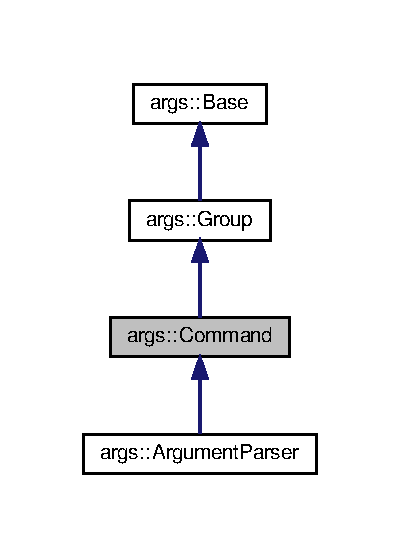
\includegraphics[width=192pt]{classargs_1_1_command__inherit__graph}
\end{center}
\end{figure}


Collaboration diagram for args\+:\+:Command\+:\nopagebreak
\begin{figure}[H]
\begin{center}
\leavevmode
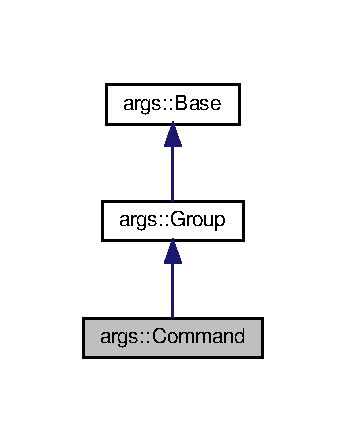
\includegraphics[width=166pt]{classargs_1_1_command__coll__graph}
\end{center}
\end{figure}
\subsection*{Classes}
\begin{DoxyCompactItemize}
\item 
class \hyperlink{classargs_1_1_command_1_1_raii_subparser}{Raii\+Subparser}
\end{DoxyCompactItemize}
\subsection*{Public Member Functions}
\begin{DoxyCompactItemize}
\item 
\hyperlink{classargs_1_1_command_a181c94ddb38711478ec718ef17d4ad36}{Command} (\hyperlink{classargs_1_1_group}{Group} \&base\+\_\+, std\+::string name\+\_\+, std\+::string help\+\_\+, std\+::function$<$ void(\hyperlink{classargs_1_1_subparser}{Subparser} \&)$>$ coroutine\+\_\+=\{\})
\item 
const std\+::string \& \hyperlink{classargs_1_1_command_a19e418cd5e8ad19f168c9e0eb6216775}{Progline\+Postfix} () const
\item 
void \hyperlink{classargs_1_1_command_a806f2aa27383139b85880f42c2de56c6}{Progline\+Postfix} (const std\+::string \&progline\+Postfix\+\_\+)
\item 
const std\+::string \& \hyperlink{classargs_1_1_command_a01d237dc3c13323c143073dd2a1a2cb4}{Description} () const
\item 
void \hyperlink{classargs_1_1_command_a4ee8820d1d6d17b10a01a5cbccce1df8}{Description} (const std\+::string \&description\+\_\+)
\item 
const std\+::string \& \hyperlink{classargs_1_1_command_a874b615da38bb03c42a5fdf281ca9e32}{Epilog} () const
\item 
void \hyperlink{classargs_1_1_command_a7364bfcd513d8f345e1bab5f3371d02d}{Epilog} (const std\+::string \&epilog\+\_\+)
\item 
const std\+::string \& \hyperlink{classargs_1_1_command_a98724f5317b07197721807ab40ca8eae}{Name} () const
\item 
const std\+::string \& \hyperlink{classargs_1_1_command_a120a9143ffb5623db08c07564e1529fc}{Help} () const
\item 
void \hyperlink{classargs_1_1_command_afbbca5178a6c712f9ad0777b7bef08bd}{Require\+Command} (bool value)
\item 
virtual bool \hyperlink{classargs_1_1_command_acc75daa42b98b9be35718f072a46f13a}{Is\+Group} () const override
\item 
virtual bool \hyperlink{classargs_1_1_command_aebb9c512301e7f0c49689ed92568ef6e}{Matched} () const noexcept override
\item 
\hyperlink{classargs_1_1_command_a31dfb353bcab4047be1dee1d915dbc8f}{operator bool} () const noexcept
\item 
void \hyperlink{classargs_1_1_command_a9a7ba5cc30681d7f5316d533637a21ba}{Match} () noexcept
\item 
void \hyperlink{classargs_1_1_command_a6c78467ab5b58df69073da9878cc783c}{Select\+Command} (\hyperlink{classargs_1_1_command}{Command} $\ast$c) noexcept
\item 
virtual \hyperlink{classargs_1_1_flag_base}{Flag\+Base} $\ast$ \hyperlink{classargs_1_1_command_ace018e92977b0e6ec5472cae0166523c}{Match} (const \hyperlink{structargs_1_1_either_flag}{Either\+Flag} \&flag) override
\item 
virtual \hyperlink{classargs_1_1_positional_base}{Positional\+Base} $\ast$ \hyperlink{classargs_1_1_command_a073266d188b3592f745c64567e566f8a}{Get\+Next\+Positional} () override
\item 
virtual bool \hyperlink{classargs_1_1_command_abcf9fafcb1531d3c0ea8a1b3a31c6ba4}{Has\+Flag} () const override
\item 
virtual bool \hyperlink{classargs_1_1_command_a5c430c5f36d678e80420d2f094ac3a4d}{Has\+Positional} () const override
\item 
virtual bool \hyperlink{classargs_1_1_command_aa7117d38f553f127542434f6cafc2697}{Has\+Command} () const override
\item 
std\+::vector$<$ std\+::string $>$ \hyperlink{classargs_1_1_command_aafb4485ab3ff22ee4d52339e098647c6}{Get\+Command\+Program\+Line} (const \hyperlink{structargs_1_1_help_params}{Help\+Params} \&params) const
\item 
virtual std\+::vector$<$ std\+::string $>$ \hyperlink{classargs_1_1_command_a37fbbde216ce232279e04edce12c1245}{Get\+Program\+Line} (const \hyperlink{structargs_1_1_help_params}{Help\+Params} \&params) const override
\item 
virtual std\+::vector$<$ \hyperlink{classargs_1_1_command}{Command} $\ast$ $>$ \hyperlink{classargs_1_1_command_a59511be164aa3a0cc5fbbfb75ca79fec}{Get\+Commands} () override
\item 
virtual std\+::vector$<$ std\+::tuple$<$ std\+::string, std\+::string, unsigned $>$ $>$ \hyperlink{classargs_1_1_command_afdd0a3ea344a4a5672565d1f2f0157f1}{Get\+Description} (const \hyperlink{structargs_1_1_help_params}{Help\+Params} \&params, const unsigned int indent) const override
\item 
virtual void \hyperlink{classargs_1_1_command_ad39b397a91af426f0ecbda9d29d7bbe0}{Validate} (const std\+::string \&shortprefix, const std\+::string \&longprefix) const override
\item 
virtual void \hyperlink{classargs_1_1_command_aa1829501dd4f63ba3551bf85171be83e}{Reset} () noexcept override
\end{DoxyCompactItemize}
\subsection*{Protected Member Functions}
\begin{DoxyCompactItemize}
\item 
\hyperlink{classargs_1_1_command_a58f55910e9746d4af64512f8e6fc6007}{Command} ()=default
\item 
std\+::function$<$ void(\hyperlink{classargs_1_1_subparser}{Subparser} \&)$>$ \& \hyperlink{classargs_1_1_command_ac026b5eeed24051bea59ff41350863d0}{Get\+Coroutine} ()
\item 
\hyperlink{classargs_1_1_command}{Command} \& \hyperlink{classargs_1_1_command_a09a64666c38476ee923b0cb7a0f56215}{Selected\+Command} ()
\item 
const \hyperlink{classargs_1_1_command}{Command} \& \hyperlink{classargs_1_1_command_af806e6bf21282670984d1ef4680d393b}{Selected\+Command} () const
\item 
void \hyperlink{classargs_1_1_command_a93c6c07576c78fabd319d8d0b872c5b1}{Update\+Subparser\+Help} (const \hyperlink{structargs_1_1_help_params}{Help\+Params} \&params) const
\end{DoxyCompactItemize}
\subsection*{Friends}
\begin{DoxyCompactItemize}
\item 
class \hyperlink{classargs_1_1_command_aecbd7c0572cb2d7fecb5eff79552c203}{Subparser}
\end{DoxyCompactItemize}
\subsection*{Additional Inherited Members}


\subsection{Detailed Description}
Main class for building subparsers.

/sa \hyperlink{classargs_1_1_subparser}{Subparser} 

\subsection{Constructor \& Destructor Documentation}
\mbox{\Hypertarget{classargs_1_1_command_a58f55910e9746d4af64512f8e6fc6007}\label{classargs_1_1_command_a58f55910e9746d4af64512f8e6fc6007}} 
\index{args\+::\+Command@{args\+::\+Command}!Command@{Command}}
\index{Command@{Command}!args\+::\+Command@{args\+::\+Command}}
\subsubsection{\texorpdfstring{Command()}{Command()}\hspace{0.1cm}{\footnotesize\ttfamily [1/2]}}
{\footnotesize\ttfamily args\+::\+Command\+::\+Command (\begin{DoxyParamCaption}{ }\end{DoxyParamCaption})\hspace{0.3cm}{\ttfamily [protected]}, {\ttfamily [default]}}

\mbox{\Hypertarget{classargs_1_1_command_a181c94ddb38711478ec718ef17d4ad36}\label{classargs_1_1_command_a181c94ddb38711478ec718ef17d4ad36}} 
\index{args\+::\+Command@{args\+::\+Command}!Command@{Command}}
\index{Command@{Command}!args\+::\+Command@{args\+::\+Command}}
\subsubsection{\texorpdfstring{Command()}{Command()}\hspace{0.1cm}{\footnotesize\ttfamily [2/2]}}
{\footnotesize\ttfamily args\+::\+Command\+::\+Command (\begin{DoxyParamCaption}\item[{\hyperlink{classargs_1_1_group}{Group} \&}]{base\+\_\+,  }\item[{std\+::string}]{name\+\_\+,  }\item[{std\+::string}]{help\+\_\+,  }\item[{std\+::function$<$ void(\hyperlink{classargs_1_1_subparser}{Subparser} \&)$>$}]{coroutine\+\_\+ = {\ttfamily \{\}} }\end{DoxyParamCaption})\hspace{0.3cm}{\ttfamily [inline]}}



\subsection{Member Function Documentation}
\mbox{\Hypertarget{classargs_1_1_command_a01d237dc3c13323c143073dd2a1a2cb4}\label{classargs_1_1_command_a01d237dc3c13323c143073dd2a1a2cb4}} 
\index{args\+::\+Command@{args\+::\+Command}!Description@{Description}}
\index{Description@{Description}!args\+::\+Command@{args\+::\+Command}}
\subsubsection{\texorpdfstring{Description()}{Description()}\hspace{0.1cm}{\footnotesize\ttfamily [1/2]}}
{\footnotesize\ttfamily const std\+::string\& args\+::\+Command\+::\+Description (\begin{DoxyParamCaption}{ }\end{DoxyParamCaption}) const\hspace{0.3cm}{\ttfamily [inline]}}

The description that appears above options \mbox{\Hypertarget{classargs_1_1_command_a4ee8820d1d6d17b10a01a5cbccce1df8}\label{classargs_1_1_command_a4ee8820d1d6d17b10a01a5cbccce1df8}} 
\index{args\+::\+Command@{args\+::\+Command}!Description@{Description}}
\index{Description@{Description}!args\+::\+Command@{args\+::\+Command}}
\subsubsection{\texorpdfstring{Description()}{Description()}\hspace{0.1cm}{\footnotesize\ttfamily [2/2]}}
{\footnotesize\ttfamily void args\+::\+Command\+::\+Description (\begin{DoxyParamCaption}\item[{const std\+::string \&}]{description\+\_\+ }\end{DoxyParamCaption})\hspace{0.3cm}{\ttfamily [inline]}}

The description that appears above options \mbox{\Hypertarget{classargs_1_1_command_a874b615da38bb03c42a5fdf281ca9e32}\label{classargs_1_1_command_a874b615da38bb03c42a5fdf281ca9e32}} 
\index{args\+::\+Command@{args\+::\+Command}!Epilog@{Epilog}}
\index{Epilog@{Epilog}!args\+::\+Command@{args\+::\+Command}}
\subsubsection{\texorpdfstring{Epilog()}{Epilog()}\hspace{0.1cm}{\footnotesize\ttfamily [1/2]}}
{\footnotesize\ttfamily const std\+::string\& args\+::\+Command\+::\+Epilog (\begin{DoxyParamCaption}{ }\end{DoxyParamCaption}) const\hspace{0.3cm}{\ttfamily [inline]}}

The description that appears below options \mbox{\Hypertarget{classargs_1_1_command_a7364bfcd513d8f345e1bab5f3371d02d}\label{classargs_1_1_command_a7364bfcd513d8f345e1bab5f3371d02d}} 
\index{args\+::\+Command@{args\+::\+Command}!Epilog@{Epilog}}
\index{Epilog@{Epilog}!args\+::\+Command@{args\+::\+Command}}
\subsubsection{\texorpdfstring{Epilog()}{Epilog()}\hspace{0.1cm}{\footnotesize\ttfamily [2/2]}}
{\footnotesize\ttfamily void args\+::\+Command\+::\+Epilog (\begin{DoxyParamCaption}\item[{const std\+::string \&}]{epilog\+\_\+ }\end{DoxyParamCaption})\hspace{0.3cm}{\ttfamily [inline]}}

The description that appears below options \mbox{\Hypertarget{classargs_1_1_command_aafb4485ab3ff22ee4d52339e098647c6}\label{classargs_1_1_command_aafb4485ab3ff22ee4d52339e098647c6}} 
\index{args\+::\+Command@{args\+::\+Command}!Get\+Command\+Program\+Line@{Get\+Command\+Program\+Line}}
\index{Get\+Command\+Program\+Line@{Get\+Command\+Program\+Line}!args\+::\+Command@{args\+::\+Command}}
\subsubsection{\texorpdfstring{Get\+Command\+Program\+Line()}{GetCommandProgramLine()}}
{\footnotesize\ttfamily std\+::vector$<$std\+::string$>$ args\+::\+Command\+::\+Get\+Command\+Program\+Line (\begin{DoxyParamCaption}\item[{const \hyperlink{structargs_1_1_help_params}{Help\+Params} \&}]{params }\end{DoxyParamCaption}) const\hspace{0.3cm}{\ttfamily [inline]}}

\mbox{\Hypertarget{classargs_1_1_command_a59511be164aa3a0cc5fbbfb75ca79fec}\label{classargs_1_1_command_a59511be164aa3a0cc5fbbfb75ca79fec}} 
\index{args\+::\+Command@{args\+::\+Command}!Get\+Commands@{Get\+Commands}}
\index{Get\+Commands@{Get\+Commands}!args\+::\+Command@{args\+::\+Command}}
\subsubsection{\texorpdfstring{Get\+Commands()}{GetCommands()}}
{\footnotesize\ttfamily virtual std\+::vector$<$\hyperlink{classargs_1_1_command}{Command}$\ast$$>$ args\+::\+Command\+::\+Get\+Commands (\begin{DoxyParamCaption}{ }\end{DoxyParamCaption})\hspace{0.3cm}{\ttfamily [inline]}, {\ttfamily [override]}, {\ttfamily [virtual]}}



Reimplemented from \hyperlink{classargs_1_1_group_a83b0a40e16d92c0f387d00a0f35dbf17}{args\+::\+Group}.

\mbox{\Hypertarget{classargs_1_1_command_ac026b5eeed24051bea59ff41350863d0}\label{classargs_1_1_command_ac026b5eeed24051bea59ff41350863d0}} 
\index{args\+::\+Command@{args\+::\+Command}!Get\+Coroutine@{Get\+Coroutine}}
\index{Get\+Coroutine@{Get\+Coroutine}!args\+::\+Command@{args\+::\+Command}}
\subsubsection{\texorpdfstring{Get\+Coroutine()}{GetCoroutine()}}
{\footnotesize\ttfamily std\+::function$<$void(\hyperlink{classargs_1_1_subparser}{Subparser}\&)$>$\& args\+::\+Command\+::\+Get\+Coroutine (\begin{DoxyParamCaption}{ }\end{DoxyParamCaption})\hspace{0.3cm}{\ttfamily [inline]}, {\ttfamily [protected]}}

\mbox{\Hypertarget{classargs_1_1_command_afdd0a3ea344a4a5672565d1f2f0157f1}\label{classargs_1_1_command_afdd0a3ea344a4a5672565d1f2f0157f1}} 
\index{args\+::\+Command@{args\+::\+Command}!Get\+Description@{Get\+Description}}
\index{Get\+Description@{Get\+Description}!args\+::\+Command@{args\+::\+Command}}
\subsubsection{\texorpdfstring{Get\+Description()}{GetDescription()}}
{\footnotesize\ttfamily virtual std\+::vector$<$std\+::tuple$<$std\+::string, std\+::string, unsigned$>$ $>$ args\+::\+Command\+::\+Get\+Description (\begin{DoxyParamCaption}\item[{const \hyperlink{structargs_1_1_help_params}{Help\+Params} \&}]{params,  }\item[{const unsigned int}]{indent }\end{DoxyParamCaption}) const\hspace{0.3cm}{\ttfamily [inline]}, {\ttfamily [override]}, {\ttfamily [virtual]}}

Get all the child descriptions for help generation 

Reimplemented from \hyperlink{classargs_1_1_group_a57068f355d7d62316b41f7a8e2528495}{args\+::\+Group}.

\mbox{\Hypertarget{classargs_1_1_command_a073266d188b3592f745c64567e566f8a}\label{classargs_1_1_command_a073266d188b3592f745c64567e566f8a}} 
\index{args\+::\+Command@{args\+::\+Command}!Get\+Next\+Positional@{Get\+Next\+Positional}}
\index{Get\+Next\+Positional@{Get\+Next\+Positional}!args\+::\+Command@{args\+::\+Command}}
\subsubsection{\texorpdfstring{Get\+Next\+Positional()}{GetNextPositional()}}
{\footnotesize\ttfamily virtual \hyperlink{classargs_1_1_positional_base}{Positional\+Base}$\ast$ args\+::\+Command\+::\+Get\+Next\+Positional (\begin{DoxyParamCaption}{ }\end{DoxyParamCaption})\hspace{0.3cm}{\ttfamily [inline]}, {\ttfamily [override]}, {\ttfamily [virtual]}}

Get the next ready positional, or nullptr if there is none

\begin{DoxyReturn}{Returns}
the first ready \hyperlink{classargs_1_1_positional_base}{Positional\+Base} pointer, or nullptr if there is no match 
\end{DoxyReturn}


Reimplemented from \hyperlink{classargs_1_1_group_ae0fa8f5ae77fda45086e7815617ddff7}{args\+::\+Group}.

\mbox{\Hypertarget{classargs_1_1_command_a37fbbde216ce232279e04edce12c1245}\label{classargs_1_1_command_a37fbbde216ce232279e04edce12c1245}} 
\index{args\+::\+Command@{args\+::\+Command}!Get\+Program\+Line@{Get\+Program\+Line}}
\index{Get\+Program\+Line@{Get\+Program\+Line}!args\+::\+Command@{args\+::\+Command}}
\subsubsection{\texorpdfstring{Get\+Program\+Line()}{GetProgramLine()}}
{\footnotesize\ttfamily virtual std\+::vector$<$std\+::string$>$ args\+::\+Command\+::\+Get\+Program\+Line (\begin{DoxyParamCaption}\item[{const \hyperlink{structargs_1_1_help_params}{Help\+Params} \&}]{params }\end{DoxyParamCaption}) const\hspace{0.3cm}{\ttfamily [inline]}, {\ttfamily [override]}, {\ttfamily [virtual]}}

Get the names of positional parameters 

Reimplemented from \hyperlink{classargs_1_1_group_abe9ab07499ec19e941df8f38e18089df}{args\+::\+Group}.

\mbox{\Hypertarget{classargs_1_1_command_aa7117d38f553f127542434f6cafc2697}\label{classargs_1_1_command_aa7117d38f553f127542434f6cafc2697}} 
\index{args\+::\+Command@{args\+::\+Command}!Has\+Command@{Has\+Command}}
\index{Has\+Command@{Has\+Command}!args\+::\+Command@{args\+::\+Command}}
\subsubsection{\texorpdfstring{Has\+Command()}{HasCommand()}}
{\footnotesize\ttfamily virtual bool args\+::\+Command\+::\+Has\+Command (\begin{DoxyParamCaption}{ }\end{DoxyParamCaption}) const\hspace{0.3cm}{\ttfamily [inline]}, {\ttfamily [override]}, {\ttfamily [virtual]}}

Get whether this has any \hyperlink{classargs_1_1_command}{Command} children

\begin{DoxyReturn}{Returns}
Whether or not there are any \hyperlink{classargs_1_1_command}{Command} children 
\end{DoxyReturn}


Reimplemented from \hyperlink{classargs_1_1_group_a022cbdf1f4bfe4210a56fa8ca9045bf8}{args\+::\+Group}.

\mbox{\Hypertarget{classargs_1_1_command_abcf9fafcb1531d3c0ea8a1b3a31c6ba4}\label{classargs_1_1_command_abcf9fafcb1531d3c0ea8a1b3a31c6ba4}} 
\index{args\+::\+Command@{args\+::\+Command}!Has\+Flag@{Has\+Flag}}
\index{Has\+Flag@{Has\+Flag}!args\+::\+Command@{args\+::\+Command}}
\subsubsection{\texorpdfstring{Has\+Flag()}{HasFlag()}}
{\footnotesize\ttfamily virtual bool args\+::\+Command\+::\+Has\+Flag (\begin{DoxyParamCaption}{ }\end{DoxyParamCaption}) const\hspace{0.3cm}{\ttfamily [inline]}, {\ttfamily [override]}, {\ttfamily [virtual]}}

Get whether this has any \hyperlink{classargs_1_1_flag_base}{Flag\+Base} children

\begin{DoxyReturn}{Returns}
Whether or not there are any \hyperlink{classargs_1_1_flag_base}{Flag\+Base} children 
\end{DoxyReturn}


Reimplemented from \hyperlink{classargs_1_1_group_a67e35305748038c175dee92ad1f5290f}{args\+::\+Group}.

\mbox{\Hypertarget{classargs_1_1_command_a5c430c5f36d678e80420d2f094ac3a4d}\label{classargs_1_1_command_a5c430c5f36d678e80420d2f094ac3a4d}} 
\index{args\+::\+Command@{args\+::\+Command}!Has\+Positional@{Has\+Positional}}
\index{Has\+Positional@{Has\+Positional}!args\+::\+Command@{args\+::\+Command}}
\subsubsection{\texorpdfstring{Has\+Positional()}{HasPositional()}}
{\footnotesize\ttfamily virtual bool args\+::\+Command\+::\+Has\+Positional (\begin{DoxyParamCaption}{ }\end{DoxyParamCaption}) const\hspace{0.3cm}{\ttfamily [inline]}, {\ttfamily [override]}, {\ttfamily [virtual]}}

Get whether this has any \hyperlink{classargs_1_1_positional_base}{Positional\+Base} children

\begin{DoxyReturn}{Returns}
Whether or not there are any \hyperlink{classargs_1_1_positional_base}{Positional\+Base} children 
\end{DoxyReturn}


Reimplemented from \hyperlink{classargs_1_1_group_a3d976f35f65ed8e4908eb88ce84accd4}{args\+::\+Group}.

\mbox{\Hypertarget{classargs_1_1_command_a120a9143ffb5623db08c07564e1529fc}\label{classargs_1_1_command_a120a9143ffb5623db08c07564e1529fc}} 
\index{args\+::\+Command@{args\+::\+Command}!Help@{Help}}
\index{Help@{Help}!args\+::\+Command@{args\+::\+Command}}
\subsubsection{\texorpdfstring{Help()}{Help()}}
{\footnotesize\ttfamily const std\+::string\& args\+::\+Command\+::\+Help (\begin{DoxyParamCaption}{ }\end{DoxyParamCaption}) const\hspace{0.3cm}{\ttfamily [inline]}}

The description of command \mbox{\Hypertarget{classargs_1_1_command_acc75daa42b98b9be35718f072a46f13a}\label{classargs_1_1_command_acc75daa42b98b9be35718f072a46f13a}} 
\index{args\+::\+Command@{args\+::\+Command}!Is\+Group@{Is\+Group}}
\index{Is\+Group@{Is\+Group}!args\+::\+Command@{args\+::\+Command}}
\subsubsection{\texorpdfstring{Is\+Group()}{IsGroup()}}
{\footnotesize\ttfamily virtual bool args\+::\+Command\+::\+Is\+Group (\begin{DoxyParamCaption}{ }\end{DoxyParamCaption}) const\hspace{0.3cm}{\ttfamily [inline]}, {\ttfamily [override]}, {\ttfamily [virtual]}}



Reimplemented from \hyperlink{classargs_1_1_group_a60de0a1db5be506a8638af0d3ce329bc}{args\+::\+Group}.

\mbox{\Hypertarget{classargs_1_1_command_a9a7ba5cc30681d7f5316d533637a21ba}\label{classargs_1_1_command_a9a7ba5cc30681d7f5316d533637a21ba}} 
\index{args\+::\+Command@{args\+::\+Command}!Match@{Match}}
\index{Match@{Match}!args\+::\+Command@{args\+::\+Command}}
\subsubsection{\texorpdfstring{Match()}{Match()}\hspace{0.1cm}{\footnotesize\ttfamily [1/2]}}
{\footnotesize\ttfamily void args\+::\+Command\+::\+Match (\begin{DoxyParamCaption}{ }\end{DoxyParamCaption})\hspace{0.3cm}{\ttfamily [inline]}, {\ttfamily [noexcept]}}

\mbox{\Hypertarget{classargs_1_1_command_ace018e92977b0e6ec5472cae0166523c}\label{classargs_1_1_command_ace018e92977b0e6ec5472cae0166523c}} 
\index{args\+::\+Command@{args\+::\+Command}!Match@{Match}}
\index{Match@{Match}!args\+::\+Command@{args\+::\+Command}}
\subsubsection{\texorpdfstring{Match()}{Match()}\hspace{0.1cm}{\footnotesize\ttfamily [2/2]}}
{\footnotesize\ttfamily virtual \hyperlink{classargs_1_1_flag_base}{Flag\+Base}$\ast$ args\+::\+Command\+::\+Match (\begin{DoxyParamCaption}\item[{const \hyperlink{structargs_1_1_either_flag}{Either\+Flag} \&}]{flag }\end{DoxyParamCaption})\hspace{0.3cm}{\ttfamily [inline]}, {\ttfamily [override]}, {\ttfamily [virtual]}}

Return the first \hyperlink{classargs_1_1_flag_base}{Flag\+Base} that matches flag, or nullptr


\begin{DoxyParams}{Parameters}
{\em flag} & The flag with prefixes stripped \\
\hline
\end{DoxyParams}
\begin{DoxyReturn}{Returns}
the first matching \hyperlink{classargs_1_1_flag_base}{Flag\+Base} pointer, or nullptr if there is no match 
\end{DoxyReturn}


Reimplemented from \hyperlink{classargs_1_1_group_a31872f412d5b32e0afaf962cd2ce5e40}{args\+::\+Group}.

\mbox{\Hypertarget{classargs_1_1_command_aebb9c512301e7f0c49689ed92568ef6e}\label{classargs_1_1_command_aebb9c512301e7f0c49689ed92568ef6e}} 
\index{args\+::\+Command@{args\+::\+Command}!Matched@{Matched}}
\index{Matched@{Matched}!args\+::\+Command@{args\+::\+Command}}
\subsubsection{\texorpdfstring{Matched()}{Matched()}}
{\footnotesize\ttfamily virtual bool args\+::\+Command\+::\+Matched (\begin{DoxyParamCaption}{ }\end{DoxyParamCaption}) const\hspace{0.3cm}{\ttfamily [inline]}, {\ttfamily [override]}, {\ttfamily [virtual]}, {\ttfamily [noexcept]}}

Whether or not this group matches validation 

Reimplemented from \hyperlink{classargs_1_1_group_a7794d31edae97254be440b8768db9af0}{args\+::\+Group}.

\mbox{\Hypertarget{classargs_1_1_command_a98724f5317b07197721807ab40ca8eae}\label{classargs_1_1_command_a98724f5317b07197721807ab40ca8eae}} 
\index{args\+::\+Command@{args\+::\+Command}!Name@{Name}}
\index{Name@{Name}!args\+::\+Command@{args\+::\+Command}}
\subsubsection{\texorpdfstring{Name()}{Name()}}
{\footnotesize\ttfamily const std\+::string\& args\+::\+Command\+::\+Name (\begin{DoxyParamCaption}{ }\end{DoxyParamCaption}) const\hspace{0.3cm}{\ttfamily [inline]}}

The name of command \mbox{\Hypertarget{classargs_1_1_command_a31dfb353bcab4047be1dee1d915dbc8f}\label{classargs_1_1_command_a31dfb353bcab4047be1dee1d915dbc8f}} 
\index{args\+::\+Command@{args\+::\+Command}!operator bool@{operator bool}}
\index{operator bool@{operator bool}!args\+::\+Command@{args\+::\+Command}}
\subsubsection{\texorpdfstring{operator bool()}{operator bool()}}
{\footnotesize\ttfamily args\+::\+Command\+::operator bool (\begin{DoxyParamCaption}{ }\end{DoxyParamCaption}) const\hspace{0.3cm}{\ttfamily [inline]}, {\ttfamily [noexcept]}}

\mbox{\Hypertarget{classargs_1_1_command_a19e418cd5e8ad19f168c9e0eb6216775}\label{classargs_1_1_command_a19e418cd5e8ad19f168c9e0eb6216775}} 
\index{args\+::\+Command@{args\+::\+Command}!Progline\+Postfix@{Progline\+Postfix}}
\index{Progline\+Postfix@{Progline\+Postfix}!args\+::\+Command@{args\+::\+Command}}
\subsubsection{\texorpdfstring{Progline\+Postfix()}{ProglinePostfix()}\hspace{0.1cm}{\footnotesize\ttfamily [1/2]}}
{\footnotesize\ttfamily const std\+::string\& args\+::\+Command\+::\+Progline\+Postfix (\begin{DoxyParamCaption}{ }\end{DoxyParamCaption}) const\hspace{0.3cm}{\ttfamily [inline]}}

The description that appears on the prog line after options \mbox{\Hypertarget{classargs_1_1_command_a806f2aa27383139b85880f42c2de56c6}\label{classargs_1_1_command_a806f2aa27383139b85880f42c2de56c6}} 
\index{args\+::\+Command@{args\+::\+Command}!Progline\+Postfix@{Progline\+Postfix}}
\index{Progline\+Postfix@{Progline\+Postfix}!args\+::\+Command@{args\+::\+Command}}
\subsubsection{\texorpdfstring{Progline\+Postfix()}{ProglinePostfix()}\hspace{0.1cm}{\footnotesize\ttfamily [2/2]}}
{\footnotesize\ttfamily void args\+::\+Command\+::\+Progline\+Postfix (\begin{DoxyParamCaption}\item[{const std\+::string \&}]{progline\+Postfix\+\_\+ }\end{DoxyParamCaption})\hspace{0.3cm}{\ttfamily [inline]}}

The description that appears on the prog line after options \mbox{\Hypertarget{classargs_1_1_command_afbbca5178a6c712f9ad0777b7bef08bd}\label{classargs_1_1_command_afbbca5178a6c712f9ad0777b7bef08bd}} 
\index{args\+::\+Command@{args\+::\+Command}!Require\+Command@{Require\+Command}}
\index{Require\+Command@{Require\+Command}!args\+::\+Command@{args\+::\+Command}}
\subsubsection{\texorpdfstring{Require\+Command()}{RequireCommand()}}
{\footnotesize\ttfamily void args\+::\+Command\+::\+Require\+Command (\begin{DoxyParamCaption}\item[{bool}]{value }\end{DoxyParamCaption})\hspace{0.3cm}{\ttfamily [inline]}}

If value is true, parser will fail if no command was parsed.

Default\+: true. \mbox{\Hypertarget{classargs_1_1_command_aa1829501dd4f63ba3551bf85171be83e}\label{classargs_1_1_command_aa1829501dd4f63ba3551bf85171be83e}} 
\index{args\+::\+Command@{args\+::\+Command}!Reset@{Reset}}
\index{Reset@{Reset}!args\+::\+Command@{args\+::\+Command}}
\subsubsection{\texorpdfstring{Reset()}{Reset()}}
{\footnotesize\ttfamily virtual void args\+::\+Command\+::\+Reset (\begin{DoxyParamCaption}{ }\end{DoxyParamCaption})\hspace{0.3cm}{\ttfamily [inline]}, {\ttfamily [override]}, {\ttfamily [virtual]}, {\ttfamily [noexcept]}}



Reimplemented from \hyperlink{classargs_1_1_group_a7ccee0f0ea0902b82029b2ab30f3f84b}{args\+::\+Group}.



Reimplemented in \hyperlink{classargs_1_1_argument_parser_a73b0dc7bc87c3a44345879f34985237f}{args\+::\+Argument\+Parser}.

\mbox{\Hypertarget{classargs_1_1_command_a6c78467ab5b58df69073da9878cc783c}\label{classargs_1_1_command_a6c78467ab5b58df69073da9878cc783c}} 
\index{args\+::\+Command@{args\+::\+Command}!Select\+Command@{Select\+Command}}
\index{Select\+Command@{Select\+Command}!args\+::\+Command@{args\+::\+Command}}
\subsubsection{\texorpdfstring{Select\+Command()}{SelectCommand()}}
{\footnotesize\ttfamily void args\+::\+Command\+::\+Select\+Command (\begin{DoxyParamCaption}\item[{\hyperlink{classargs_1_1_command}{Command} $\ast$}]{c }\end{DoxyParamCaption})\hspace{0.3cm}{\ttfamily [inline]}, {\ttfamily [noexcept]}}

\mbox{\Hypertarget{classargs_1_1_command_a09a64666c38476ee923b0cb7a0f56215}\label{classargs_1_1_command_a09a64666c38476ee923b0cb7a0f56215}} 
\index{args\+::\+Command@{args\+::\+Command}!Selected\+Command@{Selected\+Command}}
\index{Selected\+Command@{Selected\+Command}!args\+::\+Command@{args\+::\+Command}}
\subsubsection{\texorpdfstring{Selected\+Command()}{SelectedCommand()}\hspace{0.1cm}{\footnotesize\ttfamily [1/2]}}
{\footnotesize\ttfamily \hyperlink{classargs_1_1_command}{Command}\& args\+::\+Command\+::\+Selected\+Command (\begin{DoxyParamCaption}{ }\end{DoxyParamCaption})\hspace{0.3cm}{\ttfamily [inline]}, {\ttfamily [protected]}}

\mbox{\Hypertarget{classargs_1_1_command_af806e6bf21282670984d1ef4680d393b}\label{classargs_1_1_command_af806e6bf21282670984d1ef4680d393b}} 
\index{args\+::\+Command@{args\+::\+Command}!Selected\+Command@{Selected\+Command}}
\index{Selected\+Command@{Selected\+Command}!args\+::\+Command@{args\+::\+Command}}
\subsubsection{\texorpdfstring{Selected\+Command()}{SelectedCommand()}\hspace{0.1cm}{\footnotesize\ttfamily [2/2]}}
{\footnotesize\ttfamily const \hyperlink{classargs_1_1_command}{Command}\& args\+::\+Command\+::\+Selected\+Command (\begin{DoxyParamCaption}{ }\end{DoxyParamCaption}) const\hspace{0.3cm}{\ttfamily [inline]}, {\ttfamily [protected]}}

\mbox{\Hypertarget{classargs_1_1_command_a93c6c07576c78fabd319d8d0b872c5b1}\label{classargs_1_1_command_a93c6c07576c78fabd319d8d0b872c5b1}} 
\index{args\+::\+Command@{args\+::\+Command}!Update\+Subparser\+Help@{Update\+Subparser\+Help}}
\index{Update\+Subparser\+Help@{Update\+Subparser\+Help}!args\+::\+Command@{args\+::\+Command}}
\subsubsection{\texorpdfstring{Update\+Subparser\+Help()}{UpdateSubparserHelp()}}
{\footnotesize\ttfamily void args\+::\+Command\+::\+Update\+Subparser\+Help (\begin{DoxyParamCaption}\item[{const \hyperlink{structargs_1_1_help_params}{Help\+Params} \&}]{params }\end{DoxyParamCaption}) const\hspace{0.3cm}{\ttfamily [inline]}, {\ttfamily [protected]}}

\mbox{\Hypertarget{classargs_1_1_command_ad39b397a91af426f0ecbda9d29d7bbe0}\label{classargs_1_1_command_ad39b397a91af426f0ecbda9d29d7bbe0}} 
\index{args\+::\+Command@{args\+::\+Command}!Validate@{Validate}}
\index{Validate@{Validate}!args\+::\+Command@{args\+::\+Command}}
\subsubsection{\texorpdfstring{Validate()}{Validate()}}
{\footnotesize\ttfamily virtual void args\+::\+Command\+::\+Validate (\begin{DoxyParamCaption}\item[{const std\+::string \&}]{shortprefix,  }\item[{const std\+::string \&}]{longprefix }\end{DoxyParamCaption}) const\hspace{0.3cm}{\ttfamily [inline]}, {\ttfamily [override]}, {\ttfamily [virtual]}}



Reimplemented from \hyperlink{classargs_1_1_group_a9f74bb3d58e5bfe331a6af8a9981ebda}{args\+::\+Group}.



\subsection{Friends And Related Function Documentation}
\mbox{\Hypertarget{classargs_1_1_command_aecbd7c0572cb2d7fecb5eff79552c203}\label{classargs_1_1_command_aecbd7c0572cb2d7fecb5eff79552c203}} 
\index{args\+::\+Command@{args\+::\+Command}!Subparser@{Subparser}}
\index{Subparser@{Subparser}!args\+::\+Command@{args\+::\+Command}}
\subsubsection{\texorpdfstring{Subparser}{Subparser}}
{\footnotesize\ttfamily friend class \hyperlink{classargs_1_1_subparser}{Subparser}\hspace{0.3cm}{\ttfamily [friend]}}



The documentation for this class was generated from the following file\+:\begin{DoxyCompactItemize}
\item 
/home/cappelletto/github/self/landing\+\_\+area\+\_\+detector/external/\hyperlink{args_8hxx}{args.\+hxx}\end{DoxyCompactItemize}

\hypertarget{classargs_1_1_counter_flag}{}\section{args\+:\+:Counter\+Flag Class Reference}
\label{classargs_1_1_counter_flag}\index{args\+::\+Counter\+Flag@{args\+::\+Counter\+Flag}}


{\ttfamily \#include $<$args.\+hxx$>$}



Inheritance diagram for args\+:\+:Counter\+Flag\+:\nopagebreak
\begin{figure}[H]
\begin{center}
\leavevmode
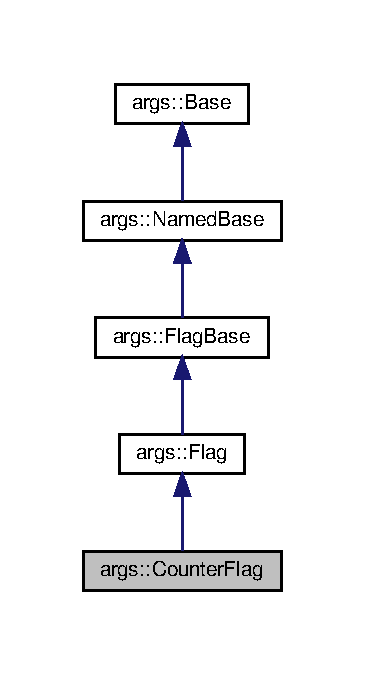
\includegraphics[width=175pt]{classargs_1_1_counter_flag__inherit__graph}
\end{center}
\end{figure}


Collaboration diagram for args\+:\+:Counter\+Flag\+:\nopagebreak
\begin{figure}[H]
\begin{center}
\leavevmode
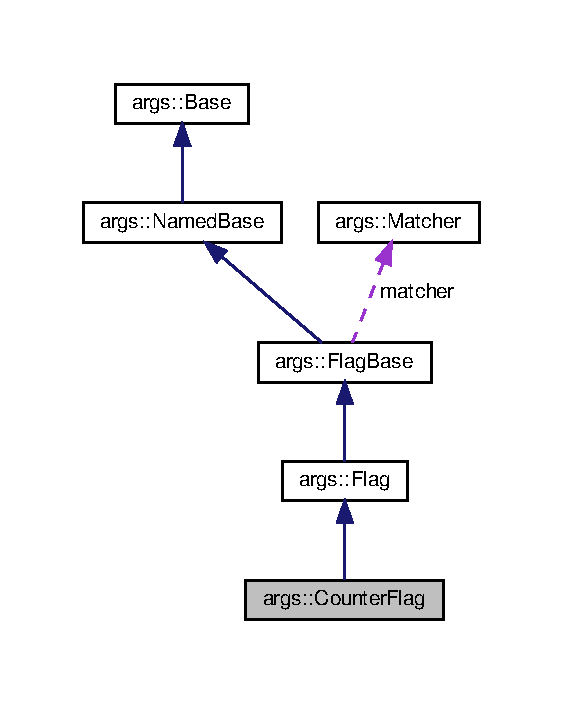
\includegraphics[width=270pt]{classargs_1_1_counter_flag__coll__graph}
\end{center}
\end{figure}
\subsection*{Public Member Functions}
\begin{DoxyCompactItemize}
\item 
\hyperlink{classargs_1_1_counter_flag_a804bc02152fef801581c150e4271089a}{Counter\+Flag} (\hyperlink{classargs_1_1_group}{Group} \&group\+\_\+, const std\+::string \&name\+\_\+, const std\+::string \&help\+\_\+, \hyperlink{classargs_1_1_matcher}{Matcher} \&\&matcher\+\_\+, const int startcount\+\_\+=0)
\item 
virtual \hyperlink{classargs_1_1_counter_flag_a3acc256cd4819c320800c57565d7c2e3}{$\sim$\+Counter\+Flag} ()
\item 
virtual \hyperlink{classargs_1_1_flag_base}{Flag\+Base} $\ast$ \hyperlink{classargs_1_1_counter_flag_ade999a8d89a8fd3db7508dfe7fdf851c}{Match} (const \hyperlink{structargs_1_1_either_flag}{Either\+Flag} \&arg) override
\item 
int \& \hyperlink{classargs_1_1_counter_flag_a74569d67e5fddf37d08614abb0df525c}{Get} () noexcept
\item 
virtual void \hyperlink{classargs_1_1_counter_flag_a408f9c2bf8f3715b89f27f23dfa2a3a5}{Reset} () noexcept override
\end{DoxyCompactItemize}
\subsection*{Additional Inherited Members}


\subsection{Detailed Description}
A flag class that simply counts the number of times it\textquotesingle{}s matched 

\subsection{Constructor \& Destructor Documentation}
\mbox{\Hypertarget{classargs_1_1_counter_flag_a804bc02152fef801581c150e4271089a}\label{classargs_1_1_counter_flag_a804bc02152fef801581c150e4271089a}} 
\index{args\+::\+Counter\+Flag@{args\+::\+Counter\+Flag}!Counter\+Flag@{Counter\+Flag}}
\index{Counter\+Flag@{Counter\+Flag}!args\+::\+Counter\+Flag@{args\+::\+Counter\+Flag}}
\subsubsection{\texorpdfstring{Counter\+Flag()}{CounterFlag()}}
{\footnotesize\ttfamily args\+::\+Counter\+Flag\+::\+Counter\+Flag (\begin{DoxyParamCaption}\item[{\hyperlink{classargs_1_1_group}{Group} \&}]{group\+\_\+,  }\item[{const std\+::string \&}]{name\+\_\+,  }\item[{const std\+::string \&}]{help\+\_\+,  }\item[{\hyperlink{classargs_1_1_matcher}{Matcher} \&\&}]{matcher\+\_\+,  }\item[{const int}]{startcount\+\_\+ = {\ttfamily 0} }\end{DoxyParamCaption})\hspace{0.3cm}{\ttfamily [inline]}}

\mbox{\Hypertarget{classargs_1_1_counter_flag_a3acc256cd4819c320800c57565d7c2e3}\label{classargs_1_1_counter_flag_a3acc256cd4819c320800c57565d7c2e3}} 
\index{args\+::\+Counter\+Flag@{args\+::\+Counter\+Flag}!````~Counter\+Flag@{$\sim$\+Counter\+Flag}}
\index{````~Counter\+Flag@{$\sim$\+Counter\+Flag}!args\+::\+Counter\+Flag@{args\+::\+Counter\+Flag}}
\subsubsection{\texorpdfstring{$\sim$\+Counter\+Flag()}{~CounterFlag()}}
{\footnotesize\ttfamily virtual args\+::\+Counter\+Flag\+::$\sim$\+Counter\+Flag (\begin{DoxyParamCaption}{ }\end{DoxyParamCaption})\hspace{0.3cm}{\ttfamily [inline]}, {\ttfamily [virtual]}}



\subsection{Member Function Documentation}
\mbox{\Hypertarget{classargs_1_1_counter_flag_a74569d67e5fddf37d08614abb0df525c}\label{classargs_1_1_counter_flag_a74569d67e5fddf37d08614abb0df525c}} 
\index{args\+::\+Counter\+Flag@{args\+::\+Counter\+Flag}!Get@{Get}}
\index{Get@{Get}!args\+::\+Counter\+Flag@{args\+::\+Counter\+Flag}}
\subsubsection{\texorpdfstring{Get()}{Get()}}
{\footnotesize\ttfamily int\& args\+::\+Counter\+Flag\+::\+Get (\begin{DoxyParamCaption}{ }\end{DoxyParamCaption})\hspace{0.3cm}{\ttfamily [inline]}, {\ttfamily [noexcept]}}

Get the count \mbox{\Hypertarget{classargs_1_1_counter_flag_ade999a8d89a8fd3db7508dfe7fdf851c}\label{classargs_1_1_counter_flag_ade999a8d89a8fd3db7508dfe7fdf851c}} 
\index{args\+::\+Counter\+Flag@{args\+::\+Counter\+Flag}!Match@{Match}}
\index{Match@{Match}!args\+::\+Counter\+Flag@{args\+::\+Counter\+Flag}}
\subsubsection{\texorpdfstring{Match()}{Match()}}
{\footnotesize\ttfamily virtual \hyperlink{classargs_1_1_flag_base}{Flag\+Base}$\ast$ args\+::\+Counter\+Flag\+::\+Match (\begin{DoxyParamCaption}\item[{const \hyperlink{structargs_1_1_either_flag}{Either\+Flag} \&}]{arg }\end{DoxyParamCaption})\hspace{0.3cm}{\ttfamily [inline]}, {\ttfamily [override]}, {\ttfamily [virtual]}}



Reimplemented from \hyperlink{classargs_1_1_flag_base_a729ebb681d373f09875abb2e04f820f2}{args\+::\+Flag\+Base}.

\mbox{\Hypertarget{classargs_1_1_counter_flag_a408f9c2bf8f3715b89f27f23dfa2a3a5}\label{classargs_1_1_counter_flag_a408f9c2bf8f3715b89f27f23dfa2a3a5}} 
\index{args\+::\+Counter\+Flag@{args\+::\+Counter\+Flag}!Reset@{Reset}}
\index{Reset@{Reset}!args\+::\+Counter\+Flag@{args\+::\+Counter\+Flag}}
\subsubsection{\texorpdfstring{Reset()}{Reset()}}
{\footnotesize\ttfamily virtual void args\+::\+Counter\+Flag\+::\+Reset (\begin{DoxyParamCaption}{ }\end{DoxyParamCaption})\hspace{0.3cm}{\ttfamily [inline]}, {\ttfamily [override]}, {\ttfamily [virtual]}, {\ttfamily [noexcept]}}



Reimplemented from \hyperlink{classargs_1_1_base_ac7cfc851174f71e00173121d3013dab1}{args\+::\+Base}.



The documentation for this class was generated from the following file\+:\begin{DoxyCompactItemize}
\item 
/home/cappelletto/github/self/landing\+\_\+area\+\_\+detector/external/\hyperlink{args_8hxx}{args.\+hxx}\end{DoxyCompactItemize}

\hypertarget{structargs_1_1detail_1_1_is_convertable_to_string_3_01_t_00_01decltype_07std_1_1declval_3_01std_17020eddea127ea35668e82953e3d8bb}{}\section{args\+:\+:detail\+:\+:declval$<$ std\+:\+:ostringstream \& $>$()$<$$<$ std\+:\+:declval$<$ T $>$(), int())$>$ Struct Template Reference}
\label{structargs_1_1detail_1_1_is_convertable_to_string_3_01_t_00_01decltype_07std_1_1declval_3_01std_17020eddea127ea35668e82953e3d8bb}\index{args\+::detail\+::declval$<$ std\+::ostringstream \& $>$()$<$$<$ std\+::declval$<$ T $>$(), int())$>$@{args\+::detail\+::declval$<$ std\+::ostringstream \& $>$()$<$$<$ std\+::declval$<$ T $>$(), int())$>$}}


{\ttfamily \#include $<$args.\+hxx$>$}



Inheritance diagram for args\+:\+:detail\+:\+:declval$<$ std\+:\+:ostringstream \& $>$()$<$$<$ std\+:\+:declval$<$ T $>$(), int())$>$\+:\nopagebreak
\begin{figure}[H]
\begin{center}
\leavevmode
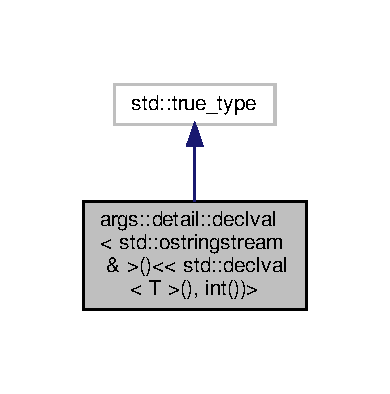
\includegraphics[width=187pt]{structargs_1_1detail_1_1_is_convertable_to_string_3_01_t_00_01decltype_07std_1_1declval_3_01std_d241314a81ccccd714662290b09817f7}
\end{center}
\end{figure}


Collaboration diagram for args\+:\+:detail\+:\+:declval$<$ std\+:\+:ostringstream \& $>$()$<$$<$ std\+:\+:declval$<$ T $>$(), int())$>$\+:\nopagebreak
\begin{figure}[H]
\begin{center}
\leavevmode
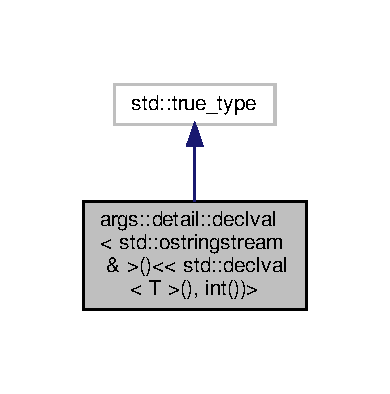
\includegraphics[width=187pt]{structargs_1_1detail_1_1_is_convertable_to_string_3_01_t_00_01decltype_07std_1_1declval_3_01std_007c5f510ea472af626d078fe6442af9}
\end{center}
\end{figure}


The documentation for this struct was generated from the following file\+:\begin{DoxyCompactItemize}
\item 
/home/cappelletto/github/self/landing\+\_\+area\+\_\+detector/external/\hyperlink{args_8hxx}{args.\+hxx}\end{DoxyCompactItemize}

\hypertarget{structargs_1_1_either_flag}{}\section{args\+:\+:Either\+Flag Struct Reference}
\label{structargs_1_1_either_flag}\index{args\+::\+Either\+Flag@{args\+::\+Either\+Flag}}


{\ttfamily \#include $<$args.\+hxx$>$}

\subsection*{Public Member Functions}
\begin{DoxyCompactItemize}
\item 
\hyperlink{structargs_1_1_either_flag_a25a55dc23248b1862616ee6d405d1cbf}{Either\+Flag} (const std\+::string \&flag)
\item 
\hyperlink{structargs_1_1_either_flag_ac1261a33bb7ff7b84b713bcd1b820cdc}{Either\+Flag} (const char $\ast$flag)
\item 
\hyperlink{structargs_1_1_either_flag_a31cca668129ae2921fbed0b5e92a8603}{Either\+Flag} (const char flag)
\item 
std\+::string \hyperlink{structargs_1_1_either_flag_a5a758d897d6bc46aac191025cdeba164}{str} () const
\item 
std\+::string \hyperlink{structargs_1_1_either_flag_ad10840d40ae21e3d14daa02db4c2e32d}{str} (const std\+::string \&short\+Prefix, const std\+::string \&long\+Prefix) const
\end{DoxyCompactItemize}
\subsection*{Static Public Member Functions}
\begin{DoxyCompactItemize}
\item 
static std\+::unordered\+\_\+set$<$ std\+::string $>$ \hyperlink{structargs_1_1_either_flag_adfbd76246674351b77adadb99c1f961e}{Get\+Long} (std\+::initializer\+\_\+list$<$ \hyperlink{structargs_1_1_either_flag}{Either\+Flag} $>$ flags)
\item 
static std\+::unordered\+\_\+set$<$ char $>$ \hyperlink{structargs_1_1_either_flag_ae08b6f663ad7f00b441443a2376411e9}{Get\+Short} (std\+::initializer\+\_\+list$<$ \hyperlink{structargs_1_1_either_flag}{Either\+Flag} $>$ flags)
\end{DoxyCompactItemize}
\subsection*{Public Attributes}
\begin{DoxyCompactItemize}
\item 
const bool \hyperlink{structargs_1_1_either_flag_afada1f6945d0f18233f9fe1466e94137}{is\+Short}
\item 
const char \hyperlink{structargs_1_1_either_flag_a27c44f6c6d1fbd96005a3d293ff2d4e2}{short\+Flag}
\item 
const std\+::string \hyperlink{structargs_1_1_either_flag_a8ae948a28b5919e82d2bbcfc999c5dda}{long\+Flag}
\end{DoxyCompactItemize}


\subsection{Detailed Description}
A simple unified option type for unified initializer lists for the \hyperlink{classargs_1_1_matcher}{Matcher} class. 

\subsection{Constructor \& Destructor Documentation}
\mbox{\Hypertarget{structargs_1_1_either_flag_a25a55dc23248b1862616ee6d405d1cbf}\label{structargs_1_1_either_flag_a25a55dc23248b1862616ee6d405d1cbf}} 
\index{args\+::\+Either\+Flag@{args\+::\+Either\+Flag}!Either\+Flag@{Either\+Flag}}
\index{Either\+Flag@{Either\+Flag}!args\+::\+Either\+Flag@{args\+::\+Either\+Flag}}
\subsubsection{\texorpdfstring{Either\+Flag()}{EitherFlag()}\hspace{0.1cm}{\footnotesize\ttfamily [1/3]}}
{\footnotesize\ttfamily args\+::\+Either\+Flag\+::\+Either\+Flag (\begin{DoxyParamCaption}\item[{const std\+::string \&}]{flag }\end{DoxyParamCaption})\hspace{0.3cm}{\ttfamily [inline]}}

\mbox{\Hypertarget{structargs_1_1_either_flag_ac1261a33bb7ff7b84b713bcd1b820cdc}\label{structargs_1_1_either_flag_ac1261a33bb7ff7b84b713bcd1b820cdc}} 
\index{args\+::\+Either\+Flag@{args\+::\+Either\+Flag}!Either\+Flag@{Either\+Flag}}
\index{Either\+Flag@{Either\+Flag}!args\+::\+Either\+Flag@{args\+::\+Either\+Flag}}
\subsubsection{\texorpdfstring{Either\+Flag()}{EitherFlag()}\hspace{0.1cm}{\footnotesize\ttfamily [2/3]}}
{\footnotesize\ttfamily args\+::\+Either\+Flag\+::\+Either\+Flag (\begin{DoxyParamCaption}\item[{const char $\ast$}]{flag }\end{DoxyParamCaption})\hspace{0.3cm}{\ttfamily [inline]}}

\mbox{\Hypertarget{structargs_1_1_either_flag_a31cca668129ae2921fbed0b5e92a8603}\label{structargs_1_1_either_flag_a31cca668129ae2921fbed0b5e92a8603}} 
\index{args\+::\+Either\+Flag@{args\+::\+Either\+Flag}!Either\+Flag@{Either\+Flag}}
\index{Either\+Flag@{Either\+Flag}!args\+::\+Either\+Flag@{args\+::\+Either\+Flag}}
\subsubsection{\texorpdfstring{Either\+Flag()}{EitherFlag()}\hspace{0.1cm}{\footnotesize\ttfamily [3/3]}}
{\footnotesize\ttfamily args\+::\+Either\+Flag\+::\+Either\+Flag (\begin{DoxyParamCaption}\item[{const char}]{flag }\end{DoxyParamCaption})\hspace{0.3cm}{\ttfamily [inline]}}



\subsection{Member Function Documentation}
\mbox{\Hypertarget{structargs_1_1_either_flag_adfbd76246674351b77adadb99c1f961e}\label{structargs_1_1_either_flag_adfbd76246674351b77adadb99c1f961e}} 
\index{args\+::\+Either\+Flag@{args\+::\+Either\+Flag}!Get\+Long@{Get\+Long}}
\index{Get\+Long@{Get\+Long}!args\+::\+Either\+Flag@{args\+::\+Either\+Flag}}
\subsubsection{\texorpdfstring{Get\+Long()}{GetLong()}}
{\footnotesize\ttfamily static std\+::unordered\+\_\+set$<$std\+::string$>$ args\+::\+Either\+Flag\+::\+Get\+Long (\begin{DoxyParamCaption}\item[{std\+::initializer\+\_\+list$<$ \hyperlink{structargs_1_1_either_flag}{Either\+Flag} $>$}]{flags }\end{DoxyParamCaption})\hspace{0.3cm}{\ttfamily [inline]}, {\ttfamily [static]}}

Get just the long flags from an initializer list of Either\+Flags \mbox{\Hypertarget{structargs_1_1_either_flag_ae08b6f663ad7f00b441443a2376411e9}\label{structargs_1_1_either_flag_ae08b6f663ad7f00b441443a2376411e9}} 
\index{args\+::\+Either\+Flag@{args\+::\+Either\+Flag}!Get\+Short@{Get\+Short}}
\index{Get\+Short@{Get\+Short}!args\+::\+Either\+Flag@{args\+::\+Either\+Flag}}
\subsubsection{\texorpdfstring{Get\+Short()}{GetShort()}}
{\footnotesize\ttfamily static std\+::unordered\+\_\+set$<$char$>$ args\+::\+Either\+Flag\+::\+Get\+Short (\begin{DoxyParamCaption}\item[{std\+::initializer\+\_\+list$<$ \hyperlink{structargs_1_1_either_flag}{Either\+Flag} $>$}]{flags }\end{DoxyParamCaption})\hspace{0.3cm}{\ttfamily [inline]}, {\ttfamily [static]}}

Get just the short flags from an initializer list of Either\+Flags \mbox{\Hypertarget{structargs_1_1_either_flag_a5a758d897d6bc46aac191025cdeba164}\label{structargs_1_1_either_flag_a5a758d897d6bc46aac191025cdeba164}} 
\index{args\+::\+Either\+Flag@{args\+::\+Either\+Flag}!str@{str}}
\index{str@{str}!args\+::\+Either\+Flag@{args\+::\+Either\+Flag}}
\subsubsection{\texorpdfstring{str()}{str()}\hspace{0.1cm}{\footnotesize\ttfamily [1/2]}}
{\footnotesize\ttfamily std\+::string args\+::\+Either\+Flag\+::str (\begin{DoxyParamCaption}{ }\end{DoxyParamCaption}) const\hspace{0.3cm}{\ttfamily [inline]}}

\mbox{\Hypertarget{structargs_1_1_either_flag_ad10840d40ae21e3d14daa02db4c2e32d}\label{structargs_1_1_either_flag_ad10840d40ae21e3d14daa02db4c2e32d}} 
\index{args\+::\+Either\+Flag@{args\+::\+Either\+Flag}!str@{str}}
\index{str@{str}!args\+::\+Either\+Flag@{args\+::\+Either\+Flag}}
\subsubsection{\texorpdfstring{str()}{str()}\hspace{0.1cm}{\footnotesize\ttfamily [2/2]}}
{\footnotesize\ttfamily std\+::string args\+::\+Either\+Flag\+::str (\begin{DoxyParamCaption}\item[{const std\+::string \&}]{short\+Prefix,  }\item[{const std\+::string \&}]{long\+Prefix }\end{DoxyParamCaption}) const\hspace{0.3cm}{\ttfamily [inline]}}



\subsection{Member Data Documentation}
\mbox{\Hypertarget{structargs_1_1_either_flag_afada1f6945d0f18233f9fe1466e94137}\label{structargs_1_1_either_flag_afada1f6945d0f18233f9fe1466e94137}} 
\index{args\+::\+Either\+Flag@{args\+::\+Either\+Flag}!is\+Short@{is\+Short}}
\index{is\+Short@{is\+Short}!args\+::\+Either\+Flag@{args\+::\+Either\+Flag}}
\subsubsection{\texorpdfstring{is\+Short}{isShort}}
{\footnotesize\ttfamily const bool args\+::\+Either\+Flag\+::is\+Short}

\mbox{\Hypertarget{structargs_1_1_either_flag_a8ae948a28b5919e82d2bbcfc999c5dda}\label{structargs_1_1_either_flag_a8ae948a28b5919e82d2bbcfc999c5dda}} 
\index{args\+::\+Either\+Flag@{args\+::\+Either\+Flag}!long\+Flag@{long\+Flag}}
\index{long\+Flag@{long\+Flag}!args\+::\+Either\+Flag@{args\+::\+Either\+Flag}}
\subsubsection{\texorpdfstring{long\+Flag}{longFlag}}
{\footnotesize\ttfamily const std\+::string args\+::\+Either\+Flag\+::long\+Flag}

\mbox{\Hypertarget{structargs_1_1_either_flag_a27c44f6c6d1fbd96005a3d293ff2d4e2}\label{structargs_1_1_either_flag_a27c44f6c6d1fbd96005a3d293ff2d4e2}} 
\index{args\+::\+Either\+Flag@{args\+::\+Either\+Flag}!short\+Flag@{short\+Flag}}
\index{short\+Flag@{short\+Flag}!args\+::\+Either\+Flag@{args\+::\+Either\+Flag}}
\subsubsection{\texorpdfstring{short\+Flag}{shortFlag}}
{\footnotesize\ttfamily const char args\+::\+Either\+Flag\+::short\+Flag}



The documentation for this struct was generated from the following file\+:\begin{DoxyCompactItemize}
\item 
/home/cappelletto/github/self/landing\+\_\+area\+\_\+detector/external/\hyperlink{args_8hxx}{args.\+hxx}\end{DoxyCompactItemize}

\hypertarget{classargs_1_1_error}{}\section{args\+:\+:Error Class Reference}
\label{classargs_1_1_error}\index{args\+::\+Error@{args\+::\+Error}}


{\ttfamily \#include $<$args.\+hxx$>$}



Inheritance diagram for args\+:\+:Error\+:\nopagebreak
\begin{figure}[H]
\begin{center}
\leavevmode
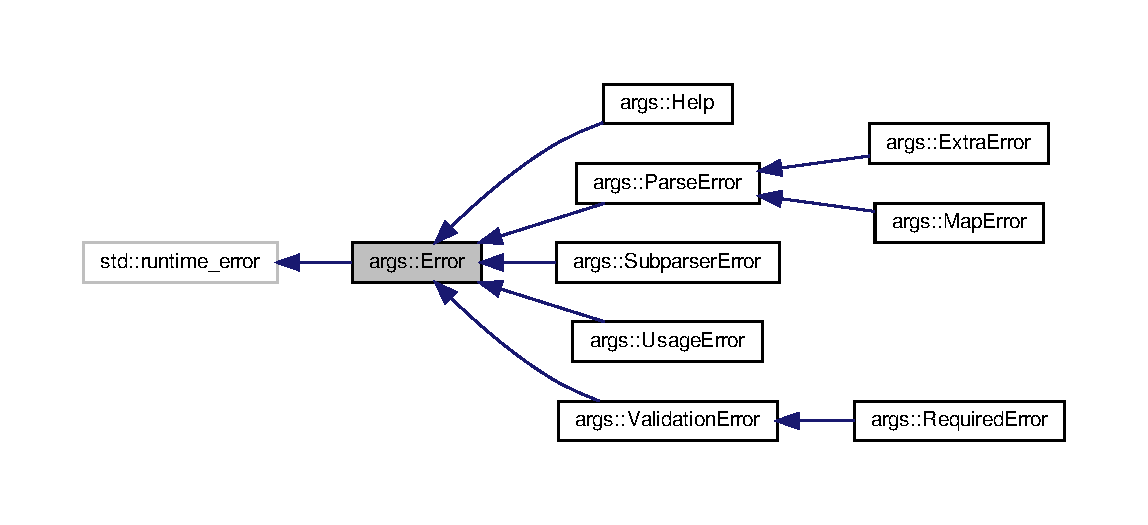
\includegraphics[width=350pt]{classargs_1_1_error__inherit__graph}
\end{center}
\end{figure}


Collaboration diagram for args\+:\+:Error\+:\nopagebreak
\begin{figure}[H]
\begin{center}
\leavevmode
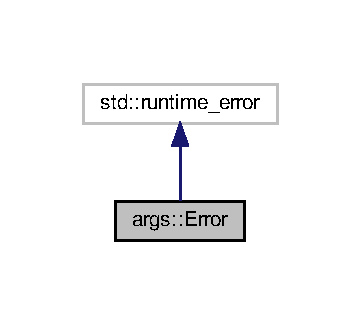
\includegraphics[width=173pt]{classargs_1_1_error__coll__graph}
\end{center}
\end{figure}
\subsection*{Public Member Functions}
\begin{DoxyCompactItemize}
\item 
\hyperlink{classargs_1_1_error_a09eff0dde2175ef1645a30ff7e93b9b0}{Error} (const std\+::string \&problem)
\item 
virtual \hyperlink{classargs_1_1_error_aab8f2900dca29d20c3d84d89b40d9ccb}{$\sim$\+Error} ()
\end{DoxyCompactItemize}


\subsection{Detailed Description}
\hyperlink{classargs_1_1_base}{Base} error class 

\subsection{Constructor \& Destructor Documentation}
\mbox{\Hypertarget{classargs_1_1_error_a09eff0dde2175ef1645a30ff7e93b9b0}\label{classargs_1_1_error_a09eff0dde2175ef1645a30ff7e93b9b0}} 
\index{args\+::\+Error@{args\+::\+Error}!Error@{Error}}
\index{Error@{Error}!args\+::\+Error@{args\+::\+Error}}
\subsubsection{\texorpdfstring{Error()}{Error()}}
{\footnotesize\ttfamily args\+::\+Error\+::\+Error (\begin{DoxyParamCaption}\item[{const std\+::string \&}]{problem }\end{DoxyParamCaption})\hspace{0.3cm}{\ttfamily [inline]}}

\mbox{\Hypertarget{classargs_1_1_error_aab8f2900dca29d20c3d84d89b40d9ccb}\label{classargs_1_1_error_aab8f2900dca29d20c3d84d89b40d9ccb}} 
\index{args\+::\+Error@{args\+::\+Error}!````~Error@{$\sim$\+Error}}
\index{````~Error@{$\sim$\+Error}!args\+::\+Error@{args\+::\+Error}}
\subsubsection{\texorpdfstring{$\sim$\+Error()}{~Error()}}
{\footnotesize\ttfamily virtual args\+::\+Error\+::$\sim$\+Error (\begin{DoxyParamCaption}{ }\end{DoxyParamCaption})\hspace{0.3cm}{\ttfamily [inline]}, {\ttfamily [virtual]}}



The documentation for this class was generated from the following file\+:\begin{DoxyCompactItemize}
\item 
/home/cappelletto/github/self/landing\+\_\+area\+\_\+detector/external/\hyperlink{args_8hxx}{args.\+hxx}\end{DoxyCompactItemize}

\hypertarget{classargs_1_1_extra_error}{}\section{args\+:\+:Extra\+Error Class Reference}
\label{classargs_1_1_extra_error}\index{args\+::\+Extra\+Error@{args\+::\+Extra\+Error}}


{\ttfamily \#include $<$args.\+hxx$>$}



Inheritance diagram for args\+:\+:Extra\+Error\+:\nopagebreak
\begin{figure}[H]
\begin{center}
\leavevmode
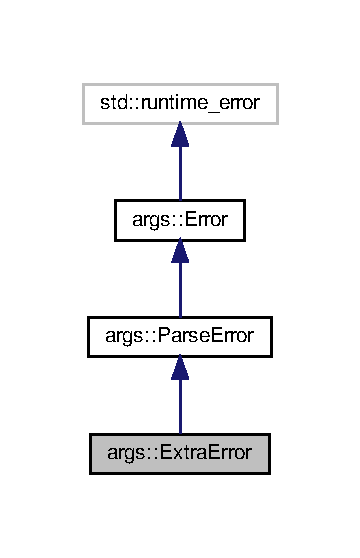
\includegraphics[width=173pt]{classargs_1_1_extra_error__inherit__graph}
\end{center}
\end{figure}


Collaboration diagram for args\+:\+:Extra\+Error\+:\nopagebreak
\begin{figure}[H]
\begin{center}
\leavevmode
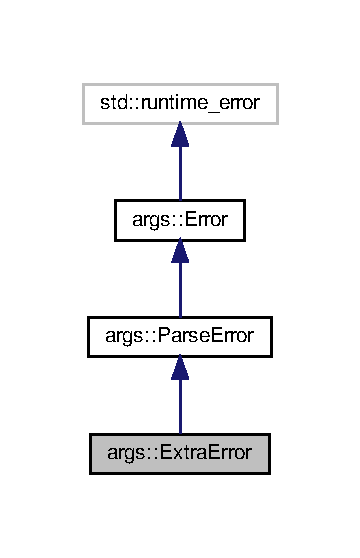
\includegraphics[width=173pt]{classargs_1_1_extra_error__coll__graph}
\end{center}
\end{figure}
\subsection*{Public Member Functions}
\begin{DoxyCompactItemize}
\item 
\hyperlink{classargs_1_1_extra_error_abfb5547b6d82444b6b7fb18d39424e97}{Extra\+Error} (const std\+::string \&problem)
\item 
virtual \hyperlink{classargs_1_1_extra_error_aeb16f55e10a446520d30ae35a1c3b174}{$\sim$\+Extra\+Error} ()
\end{DoxyCompactItemize}


\subsection{Detailed Description}
\hyperlink{classargs_1_1_error}{Error} that occurs when a singular flag is specified multiple times 

\subsection{Constructor \& Destructor Documentation}
\mbox{\Hypertarget{classargs_1_1_extra_error_abfb5547b6d82444b6b7fb18d39424e97}\label{classargs_1_1_extra_error_abfb5547b6d82444b6b7fb18d39424e97}} 
\index{args\+::\+Extra\+Error@{args\+::\+Extra\+Error}!Extra\+Error@{Extra\+Error}}
\index{Extra\+Error@{Extra\+Error}!args\+::\+Extra\+Error@{args\+::\+Extra\+Error}}
\subsubsection{\texorpdfstring{Extra\+Error()}{ExtraError()}}
{\footnotesize\ttfamily args\+::\+Extra\+Error\+::\+Extra\+Error (\begin{DoxyParamCaption}\item[{const std\+::string \&}]{problem }\end{DoxyParamCaption})\hspace{0.3cm}{\ttfamily [inline]}}

\mbox{\Hypertarget{classargs_1_1_extra_error_aeb16f55e10a446520d30ae35a1c3b174}\label{classargs_1_1_extra_error_aeb16f55e10a446520d30ae35a1c3b174}} 
\index{args\+::\+Extra\+Error@{args\+::\+Extra\+Error}!````~Extra\+Error@{$\sim$\+Extra\+Error}}
\index{````~Extra\+Error@{$\sim$\+Extra\+Error}!args\+::\+Extra\+Error@{args\+::\+Extra\+Error}}
\subsubsection{\texorpdfstring{$\sim$\+Extra\+Error()}{~ExtraError()}}
{\footnotesize\ttfamily virtual args\+::\+Extra\+Error\+::$\sim$\+Extra\+Error (\begin{DoxyParamCaption}{ }\end{DoxyParamCaption})\hspace{0.3cm}{\ttfamily [inline]}, {\ttfamily [virtual]}}



The documentation for this class was generated from the following file\+:\begin{DoxyCompactItemize}
\item 
/home/cappelletto/github/self/landing\+\_\+area\+\_\+detector/external/\hyperlink{args_8hxx}{args.\+hxx}\end{DoxyCompactItemize}

\hypertarget{classargs_1_1_flag}{}\section{args\+:\+:Flag Class Reference}
\label{classargs_1_1_flag}\index{args\+::\+Flag@{args\+::\+Flag}}


{\ttfamily \#include $<$args.\+hxx$>$}



Inheritance diagram for args\+:\+:Flag\+:\nopagebreak
\begin{figure}[H]
\begin{center}
\leavevmode
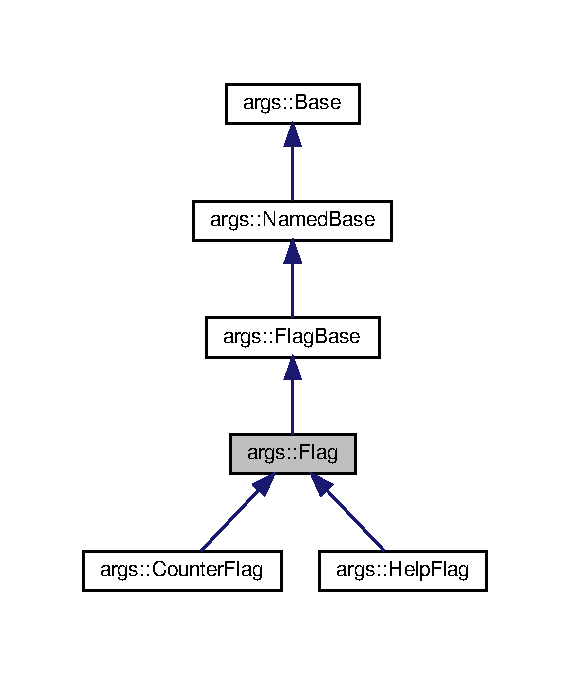
\includegraphics[width=274pt]{classargs_1_1_flag__inherit__graph}
\end{center}
\end{figure}


Collaboration diagram for args\+:\+:Flag\+:\nopagebreak
\begin{figure}[H]
\begin{center}
\leavevmode
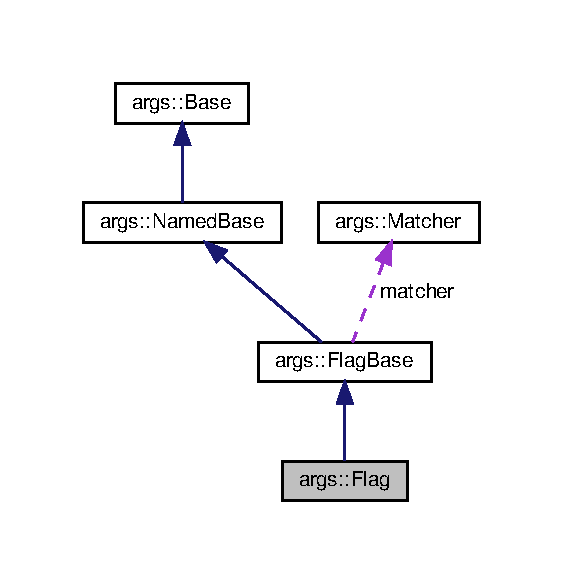
\includegraphics[width=270pt]{classargs_1_1_flag__coll__graph}
\end{center}
\end{figure}
\subsection*{Public Member Functions}
\begin{DoxyCompactItemize}
\item 
\hyperlink{classargs_1_1_flag_a49d467bbf32414fbf744f9e4a1326c4b}{Flag} (\hyperlink{classargs_1_1_group}{Group} \&group\+\_\+, const std\+::string \&name\+\_\+, const std\+::string \&help\+\_\+, \hyperlink{classargs_1_1_matcher}{Matcher} \&\&matcher\+\_\+, \hyperlink{namespaceargs_aa530c0f95194aa275f49a5f299ac9e77}{Options} options\+\_\+)
\item 
\hyperlink{classargs_1_1_flag_a42deec08baee60827d9576f56f54055c}{Flag} (\hyperlink{classargs_1_1_group}{Group} \&group\+\_\+, const std\+::string \&name\+\_\+, const std\+::string \&help\+\_\+, \hyperlink{classargs_1_1_matcher}{Matcher} \&\&matcher\+\_\+, const bool extra\+Error\+\_\+=false)
\item 
virtual \hyperlink{classargs_1_1_flag_a726b9a61e5165dd4ae1e2b67241dc761}{$\sim$\+Flag} ()
\item 
bool \hyperlink{classargs_1_1_flag_a5cdbec9617c6776ab2e3b67c0a72fd9a}{Get} () const
\item 
virtual \hyperlink{structargs_1_1_nargs}{Nargs} \hyperlink{classargs_1_1_flag_a1bd707628d2987d3ccf2dbdb810302e4}{Number\+Of\+Arguments} () const noexcept override
\item 
virtual void \hyperlink{classargs_1_1_flag_a48ce8c59b554db36d2869b24b56c94dd}{Parse\+Value} (const std\+::vector$<$ std\+::string $>$ \&) override
\end{DoxyCompactItemize}
\subsection*{Additional Inherited Members}


\subsection{Detailed Description}
Boolean argument matcher 

\subsection{Constructor \& Destructor Documentation}
\mbox{\Hypertarget{classargs_1_1_flag_a49d467bbf32414fbf744f9e4a1326c4b}\label{classargs_1_1_flag_a49d467bbf32414fbf744f9e4a1326c4b}} 
\index{args\+::\+Flag@{args\+::\+Flag}!Flag@{Flag}}
\index{Flag@{Flag}!args\+::\+Flag@{args\+::\+Flag}}
\subsubsection{\texorpdfstring{Flag()}{Flag()}\hspace{0.1cm}{\footnotesize\ttfamily [1/2]}}
{\footnotesize\ttfamily args\+::\+Flag\+::\+Flag (\begin{DoxyParamCaption}\item[{\hyperlink{classargs_1_1_group}{Group} \&}]{group\+\_\+,  }\item[{const std\+::string \&}]{name\+\_\+,  }\item[{const std\+::string \&}]{help\+\_\+,  }\item[{\hyperlink{classargs_1_1_matcher}{Matcher} \&\&}]{matcher\+\_\+,  }\item[{\hyperlink{namespaceargs_aa530c0f95194aa275f49a5f299ac9e77}{Options}}]{options\+\_\+ }\end{DoxyParamCaption})\hspace{0.3cm}{\ttfamily [inline]}}

\mbox{\Hypertarget{classargs_1_1_flag_a42deec08baee60827d9576f56f54055c}\label{classargs_1_1_flag_a42deec08baee60827d9576f56f54055c}} 
\index{args\+::\+Flag@{args\+::\+Flag}!Flag@{Flag}}
\index{Flag@{Flag}!args\+::\+Flag@{args\+::\+Flag}}
\subsubsection{\texorpdfstring{Flag()}{Flag()}\hspace{0.1cm}{\footnotesize\ttfamily [2/2]}}
{\footnotesize\ttfamily args\+::\+Flag\+::\+Flag (\begin{DoxyParamCaption}\item[{\hyperlink{classargs_1_1_group}{Group} \&}]{group\+\_\+,  }\item[{const std\+::string \&}]{name\+\_\+,  }\item[{const std\+::string \&}]{help\+\_\+,  }\item[{\hyperlink{classargs_1_1_matcher}{Matcher} \&\&}]{matcher\+\_\+,  }\item[{const bool}]{extra\+Error\+\_\+ = {\ttfamily false} }\end{DoxyParamCaption})\hspace{0.3cm}{\ttfamily [inline]}}

\mbox{\Hypertarget{classargs_1_1_flag_a726b9a61e5165dd4ae1e2b67241dc761}\label{classargs_1_1_flag_a726b9a61e5165dd4ae1e2b67241dc761}} 
\index{args\+::\+Flag@{args\+::\+Flag}!````~Flag@{$\sim$\+Flag}}
\index{````~Flag@{$\sim$\+Flag}!args\+::\+Flag@{args\+::\+Flag}}
\subsubsection{\texorpdfstring{$\sim$\+Flag()}{~Flag()}}
{\footnotesize\ttfamily virtual args\+::\+Flag\+::$\sim$\+Flag (\begin{DoxyParamCaption}{ }\end{DoxyParamCaption})\hspace{0.3cm}{\ttfamily [inline]}, {\ttfamily [virtual]}}



\subsection{Member Function Documentation}
\mbox{\Hypertarget{classargs_1_1_flag_a5cdbec9617c6776ab2e3b67c0a72fd9a}\label{classargs_1_1_flag_a5cdbec9617c6776ab2e3b67c0a72fd9a}} 
\index{args\+::\+Flag@{args\+::\+Flag}!Get@{Get}}
\index{Get@{Get}!args\+::\+Flag@{args\+::\+Flag}}
\subsubsection{\texorpdfstring{Get()}{Get()}}
{\footnotesize\ttfamily bool args\+::\+Flag\+::\+Get (\begin{DoxyParamCaption}{ }\end{DoxyParamCaption}) const\hspace{0.3cm}{\ttfamily [inline]}}

Get whether this was matched \mbox{\Hypertarget{classargs_1_1_flag_a1bd707628d2987d3ccf2dbdb810302e4}\label{classargs_1_1_flag_a1bd707628d2987d3ccf2dbdb810302e4}} 
\index{args\+::\+Flag@{args\+::\+Flag}!Number\+Of\+Arguments@{Number\+Of\+Arguments}}
\index{Number\+Of\+Arguments@{Number\+Of\+Arguments}!args\+::\+Flag@{args\+::\+Flag}}
\subsubsection{\texorpdfstring{Number\+Of\+Arguments()}{NumberOfArguments()}}
{\footnotesize\ttfamily virtual \hyperlink{structargs_1_1_nargs}{Nargs} args\+::\+Flag\+::\+Number\+Of\+Arguments (\begin{DoxyParamCaption}{ }\end{DoxyParamCaption}) const\hspace{0.3cm}{\ttfamily [inline]}, {\ttfamily [override]}, {\ttfamily [virtual]}, {\ttfamily [noexcept]}}

Defines how many values can be consumed by this option.

\begin{DoxyReturn}{Returns}
closed interval \mbox{[}min, max\mbox{]} 
\end{DoxyReturn}


Implements \hyperlink{classargs_1_1_flag_base_a6007ffeaa767893cb8eff5333d61673b}{args\+::\+Flag\+Base}.

\mbox{\Hypertarget{classargs_1_1_flag_a48ce8c59b554db36d2869b24b56c94dd}\label{classargs_1_1_flag_a48ce8c59b554db36d2869b24b56c94dd}} 
\index{args\+::\+Flag@{args\+::\+Flag}!Parse\+Value@{Parse\+Value}}
\index{Parse\+Value@{Parse\+Value}!args\+::\+Flag@{args\+::\+Flag}}
\subsubsection{\texorpdfstring{Parse\+Value()}{ParseValue()}}
{\footnotesize\ttfamily virtual void args\+::\+Flag\+::\+Parse\+Value (\begin{DoxyParamCaption}\item[{const std\+::vector$<$ std\+::string $>$ \&}]{value }\end{DoxyParamCaption})\hspace{0.3cm}{\ttfamily [inline]}, {\ttfamily [override]}, {\ttfamily [virtual]}}

Parse values of this option.


\begin{DoxyParams}{Parameters}
{\em value} & Vector of values. It\textquotesingle{}s size must be in \hyperlink{classargs_1_1_flag_a1bd707628d2987d3ccf2dbdb810302e4}{Number\+Of\+Arguments()} interval. \\
\hline
\end{DoxyParams}


Implements \hyperlink{classargs_1_1_flag_base_a3421d9a595c9426dc73f62604cdee84f}{args\+::\+Flag\+Base}.



The documentation for this class was generated from the following file\+:\begin{DoxyCompactItemize}
\item 
/home/cappelletto/github/self/landing\+\_\+area\+\_\+detector/external/\hyperlink{args_8hxx}{args.\+hxx}\end{DoxyCompactItemize}

\hypertarget{classargs_1_1_flag_base}{}\section{args\+:\+:Flag\+Base Class Reference}
\label{classargs_1_1_flag_base}\index{args\+::\+Flag\+Base@{args\+::\+Flag\+Base}}


{\ttfamily \#include $<$args.\+hxx$>$}



Inheritance diagram for args\+:\+:Flag\+Base\+:\nopagebreak
\begin{figure}[H]
\begin{center}
\leavevmode
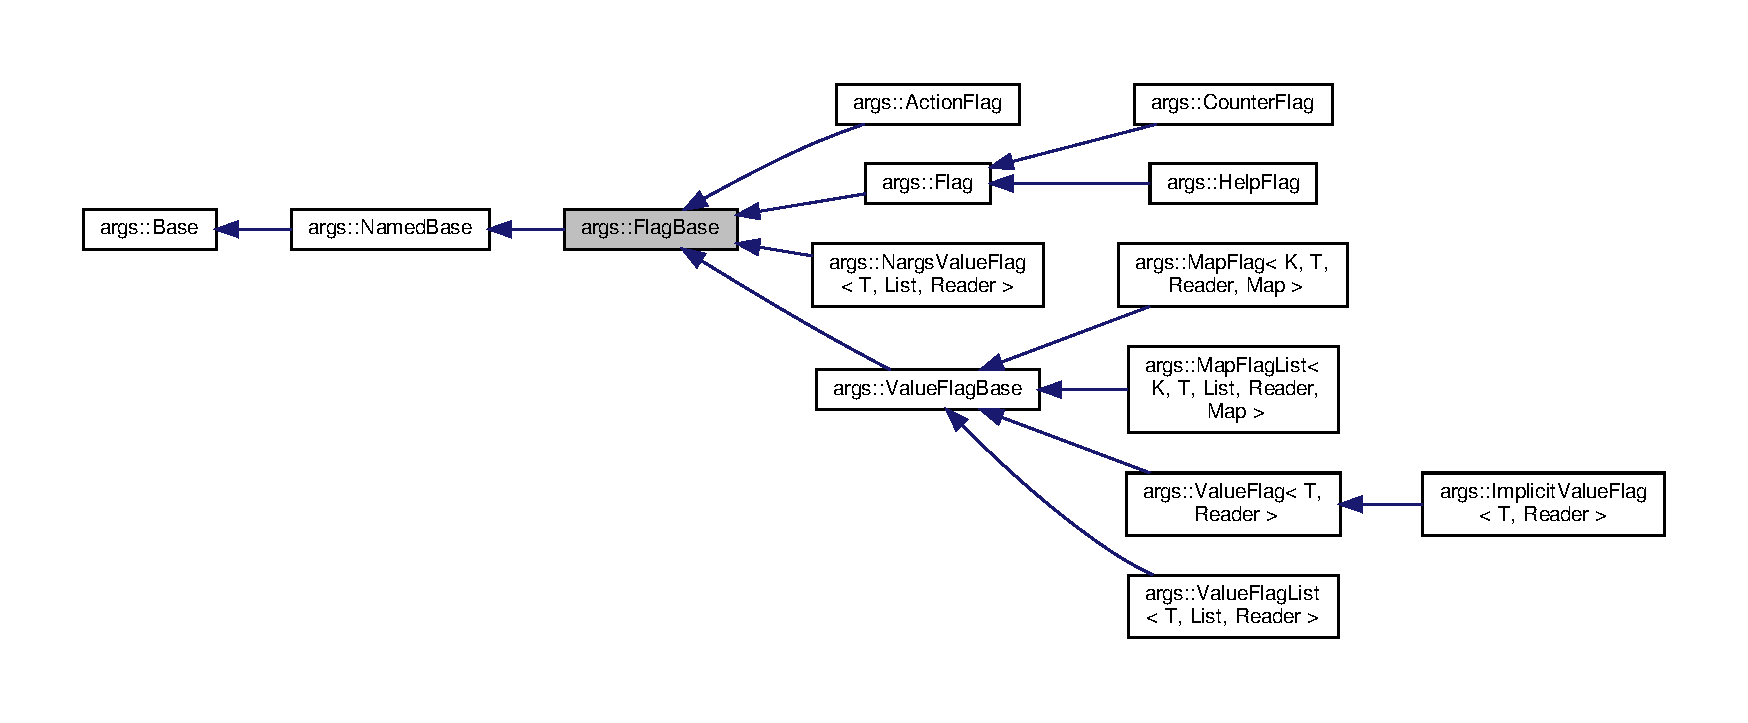
\includegraphics[width=350pt]{classargs_1_1_flag_base__inherit__graph}
\end{center}
\end{figure}


Collaboration diagram for args\+:\+:Flag\+Base\+:\nopagebreak
\begin{figure}[H]
\begin{center}
\leavevmode
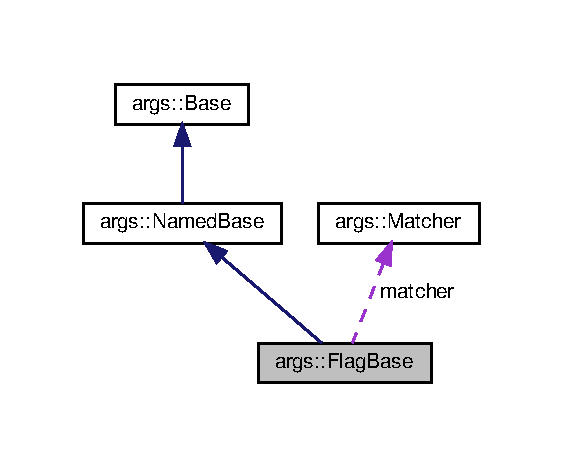
\includegraphics[width=270pt]{classargs_1_1_flag_base__coll__graph}
\end{center}
\end{figure}
\subsection*{Public Member Functions}
\begin{DoxyCompactItemize}
\item 
\hyperlink{classargs_1_1_flag_base_a9abcf8802dee008411f3b45fff44a3e1}{Flag\+Base} (const std\+::string \&name\+\_\+, const std\+::string \&help\+\_\+, \hyperlink{classargs_1_1_matcher}{Matcher} \&\&matcher\+\_\+, const bool extra\+Error\+\_\+=false)
\item 
\hyperlink{classargs_1_1_flag_base_ad99d8085ea99b778f96bad7872900d49}{Flag\+Base} (const std\+::string \&name\+\_\+, const std\+::string \&help\+\_\+, \hyperlink{classargs_1_1_matcher}{Matcher} \&\&matcher\+\_\+, \hyperlink{namespaceargs_aa530c0f95194aa275f49a5f299ac9e77}{Options} options\+\_\+)
\item 
virtual \hyperlink{classargs_1_1_flag_base_a37e287119643f8eca5eca883c3993a52}{$\sim$\+Flag\+Base} ()
\item 
virtual \hyperlink{classargs_1_1_flag_base}{Flag\+Base} $\ast$ \hyperlink{classargs_1_1_flag_base_a729ebb681d373f09875abb2e04f820f2}{Match} (const \hyperlink{structargs_1_1_either_flag}{Either\+Flag} \&flag) override
\item 
virtual void \hyperlink{classargs_1_1_flag_base_afd5a2cdea7f46caacc874c7c67ff6444}{Validate} (const std\+::string \&short\+Prefix, const std\+::string \&long\+Prefix) const override
\item 
virtual std\+::vector$<$ std\+::string $>$ \hyperlink{classargs_1_1_flag_base_aeb3153e728d38f0f3e0ea5df46fb4acc}{Get\+Program\+Line} (const \hyperlink{structargs_1_1_help_params}{Help\+Params} \&params) const override
\item 
virtual bool \hyperlink{classargs_1_1_flag_base_a67b6fa7bfd7b3ed18caeb2a6381ed1a2}{Has\+Flag} () const override
\item 
virtual \hyperlink{structargs_1_1_nargs}{Nargs} \hyperlink{classargs_1_1_flag_base_a6007ffeaa767893cb8eff5333d61673b}{Number\+Of\+Arguments} () const noexcept=0
\item 
virtual void \hyperlink{classargs_1_1_flag_base_a3421d9a595c9426dc73f62604cdee84f}{Parse\+Value} (const std\+::vector$<$ std\+::string $>$ \&value)=0
\end{DoxyCompactItemize}
\subsection*{Protected Member Functions}
\begin{DoxyCompactItemize}
\item 
virtual std\+::string \hyperlink{classargs_1_1_flag_base_a61db383104c1987904bcd331d8b3be76}{Get\+Name\+String} (const \hyperlink{structargs_1_1_help_params}{Help\+Params} \&params) const override
\end{DoxyCompactItemize}
\subsection*{Protected Attributes}
\begin{DoxyCompactItemize}
\item 
const \hyperlink{classargs_1_1_matcher}{Matcher} \hyperlink{classargs_1_1_flag_base_a8035f87d3cbd70a8a57c7a77f2c5d8f1}{matcher}
\end{DoxyCompactItemize}


\subsection{Detailed Description}
\hyperlink{classargs_1_1_base}{Base} class for all flag options 

\subsection{Constructor \& Destructor Documentation}
\mbox{\Hypertarget{classargs_1_1_flag_base_a9abcf8802dee008411f3b45fff44a3e1}\label{classargs_1_1_flag_base_a9abcf8802dee008411f3b45fff44a3e1}} 
\index{args\+::\+Flag\+Base@{args\+::\+Flag\+Base}!Flag\+Base@{Flag\+Base}}
\index{Flag\+Base@{Flag\+Base}!args\+::\+Flag\+Base@{args\+::\+Flag\+Base}}
\subsubsection{\texorpdfstring{Flag\+Base()}{FlagBase()}\hspace{0.1cm}{\footnotesize\ttfamily [1/2]}}
{\footnotesize\ttfamily args\+::\+Flag\+Base\+::\+Flag\+Base (\begin{DoxyParamCaption}\item[{const std\+::string \&}]{name\+\_\+,  }\item[{const std\+::string \&}]{help\+\_\+,  }\item[{\hyperlink{classargs_1_1_matcher}{Matcher} \&\&}]{matcher\+\_\+,  }\item[{const bool}]{extra\+Error\+\_\+ = {\ttfamily false} }\end{DoxyParamCaption})\hspace{0.3cm}{\ttfamily [inline]}}

\mbox{\Hypertarget{classargs_1_1_flag_base_ad99d8085ea99b778f96bad7872900d49}\label{classargs_1_1_flag_base_ad99d8085ea99b778f96bad7872900d49}} 
\index{args\+::\+Flag\+Base@{args\+::\+Flag\+Base}!Flag\+Base@{Flag\+Base}}
\index{Flag\+Base@{Flag\+Base}!args\+::\+Flag\+Base@{args\+::\+Flag\+Base}}
\subsubsection{\texorpdfstring{Flag\+Base()}{FlagBase()}\hspace{0.1cm}{\footnotesize\ttfamily [2/2]}}
{\footnotesize\ttfamily args\+::\+Flag\+Base\+::\+Flag\+Base (\begin{DoxyParamCaption}\item[{const std\+::string \&}]{name\+\_\+,  }\item[{const std\+::string \&}]{help\+\_\+,  }\item[{\hyperlink{classargs_1_1_matcher}{Matcher} \&\&}]{matcher\+\_\+,  }\item[{\hyperlink{namespaceargs_aa530c0f95194aa275f49a5f299ac9e77}{Options}}]{options\+\_\+ }\end{DoxyParamCaption})\hspace{0.3cm}{\ttfamily [inline]}}

\mbox{\Hypertarget{classargs_1_1_flag_base_a37e287119643f8eca5eca883c3993a52}\label{classargs_1_1_flag_base_a37e287119643f8eca5eca883c3993a52}} 
\index{args\+::\+Flag\+Base@{args\+::\+Flag\+Base}!````~Flag\+Base@{$\sim$\+Flag\+Base}}
\index{````~Flag\+Base@{$\sim$\+Flag\+Base}!args\+::\+Flag\+Base@{args\+::\+Flag\+Base}}
\subsubsection{\texorpdfstring{$\sim$\+Flag\+Base()}{~FlagBase()}}
{\footnotesize\ttfamily virtual args\+::\+Flag\+Base\+::$\sim$\+Flag\+Base (\begin{DoxyParamCaption}{ }\end{DoxyParamCaption})\hspace{0.3cm}{\ttfamily [inline]}, {\ttfamily [virtual]}}



\subsection{Member Function Documentation}
\mbox{\Hypertarget{classargs_1_1_flag_base_a61db383104c1987904bcd331d8b3be76}\label{classargs_1_1_flag_base_a61db383104c1987904bcd331d8b3be76}} 
\index{args\+::\+Flag\+Base@{args\+::\+Flag\+Base}!Get\+Name\+String@{Get\+Name\+String}}
\index{Get\+Name\+String@{Get\+Name\+String}!args\+::\+Flag\+Base@{args\+::\+Flag\+Base}}
\subsubsection{\texorpdfstring{Get\+Name\+String()}{GetNameString()}}
{\footnotesize\ttfamily virtual std\+::string args\+::\+Flag\+Base\+::\+Get\+Name\+String (\begin{DoxyParamCaption}\item[{const \hyperlink{structargs_1_1_help_params}{Help\+Params} \&}]{params }\end{DoxyParamCaption}) const\hspace{0.3cm}{\ttfamily [inline]}, {\ttfamily [override]}, {\ttfamily [protected]}, {\ttfamily [virtual]}}



Reimplemented from \hyperlink{classargs_1_1_named_base_a3c597a489d3ccc74937682407c08b3f7}{args\+::\+Named\+Base}.

\mbox{\Hypertarget{classargs_1_1_flag_base_aeb3153e728d38f0f3e0ea5df46fb4acc}\label{classargs_1_1_flag_base_aeb3153e728d38f0f3e0ea5df46fb4acc}} 
\index{args\+::\+Flag\+Base@{args\+::\+Flag\+Base}!Get\+Program\+Line@{Get\+Program\+Line}}
\index{Get\+Program\+Line@{Get\+Program\+Line}!args\+::\+Flag\+Base@{args\+::\+Flag\+Base}}
\subsubsection{\texorpdfstring{Get\+Program\+Line()}{GetProgramLine()}}
{\footnotesize\ttfamily virtual std\+::vector$<$std\+::string$>$ args\+::\+Flag\+Base\+::\+Get\+Program\+Line (\begin{DoxyParamCaption}\item[{const \hyperlink{structargs_1_1_help_params}{Help\+Params} \&}]{params }\end{DoxyParamCaption}) const\hspace{0.3cm}{\ttfamily [inline]}, {\ttfamily [override]}, {\ttfamily [virtual]}}



Reimplemented from \hyperlink{classargs_1_1_base_a88fcbbc4bfe3b7af9fafe6e96a19f337}{args\+::\+Base}.

\mbox{\Hypertarget{classargs_1_1_flag_base_a67b6fa7bfd7b3ed18caeb2a6381ed1a2}\label{classargs_1_1_flag_base_a67b6fa7bfd7b3ed18caeb2a6381ed1a2}} 
\index{args\+::\+Flag\+Base@{args\+::\+Flag\+Base}!Has\+Flag@{Has\+Flag}}
\index{Has\+Flag@{Has\+Flag}!args\+::\+Flag\+Base@{args\+::\+Flag\+Base}}
\subsubsection{\texorpdfstring{Has\+Flag()}{HasFlag()}}
{\footnotesize\ttfamily virtual bool args\+::\+Flag\+Base\+::\+Has\+Flag (\begin{DoxyParamCaption}{ }\end{DoxyParamCaption}) const\hspace{0.3cm}{\ttfamily [inline]}, {\ttfamily [override]}, {\ttfamily [virtual]}}



Reimplemented from \hyperlink{classargs_1_1_base_a81684f399665c0372439c070af5de4a7}{args\+::\+Base}.

\mbox{\Hypertarget{classargs_1_1_flag_base_a729ebb681d373f09875abb2e04f820f2}\label{classargs_1_1_flag_base_a729ebb681d373f09875abb2e04f820f2}} 
\index{args\+::\+Flag\+Base@{args\+::\+Flag\+Base}!Match@{Match}}
\index{Match@{Match}!args\+::\+Flag\+Base@{args\+::\+Flag\+Base}}
\subsubsection{\texorpdfstring{Match()}{Match()}}
{\footnotesize\ttfamily virtual \hyperlink{classargs_1_1_flag_base}{Flag\+Base}$\ast$ args\+::\+Flag\+Base\+::\+Match (\begin{DoxyParamCaption}\item[{const \hyperlink{structargs_1_1_either_flag}{Either\+Flag} \&}]{flag }\end{DoxyParamCaption})\hspace{0.3cm}{\ttfamily [inline]}, {\ttfamily [override]}, {\ttfamily [virtual]}}



Reimplemented from \hyperlink{classargs_1_1_base_a6d5a7be35d62f59fee5a52c06af3003e}{args\+::\+Base}.



Reimplemented in \hyperlink{classargs_1_1_counter_flag_ade999a8d89a8fd3db7508dfe7fdf851c}{args\+::\+Counter\+Flag}, and \hyperlink{classargs_1_1_help_flag_a1a555992a7c8350aca0ac1f292d91605}{args\+::\+Help\+Flag}.

\mbox{\Hypertarget{classargs_1_1_flag_base_a6007ffeaa767893cb8eff5333d61673b}\label{classargs_1_1_flag_base_a6007ffeaa767893cb8eff5333d61673b}} 
\index{args\+::\+Flag\+Base@{args\+::\+Flag\+Base}!Number\+Of\+Arguments@{Number\+Of\+Arguments}}
\index{Number\+Of\+Arguments@{Number\+Of\+Arguments}!args\+::\+Flag\+Base@{args\+::\+Flag\+Base}}
\subsubsection{\texorpdfstring{Number\+Of\+Arguments()}{NumberOfArguments()}}
{\footnotesize\ttfamily virtual \hyperlink{structargs_1_1_nargs}{Nargs} args\+::\+Flag\+Base\+::\+Number\+Of\+Arguments (\begin{DoxyParamCaption}{ }\end{DoxyParamCaption}) const\hspace{0.3cm}{\ttfamily [pure virtual]}, {\ttfamily [noexcept]}}

Defines how many values can be consumed by this option.

\begin{DoxyReturn}{Returns}
closed interval \mbox{[}min, max\mbox{]} 
\end{DoxyReturn}


Implemented in \hyperlink{classargs_1_1_nargs_value_flag_a8db7ce6ec0d27f649dbfb1bba908078a}{args\+::\+Nargs\+Value\+Flag$<$ T, List, Reader $>$}, \hyperlink{classargs_1_1_implicit_value_flag_a7cfc67aca2b32921e722f51d349df2c5}{args\+::\+Implicit\+Value\+Flag$<$ T, Reader $>$}, \hyperlink{classargs_1_1_action_flag_aa341976acd895df15fb2bfe7182c48eb}{args\+::\+Action\+Flag}, \hyperlink{classargs_1_1_flag_a1bd707628d2987d3ccf2dbdb810302e4}{args\+::\+Flag}, and \hyperlink{classargs_1_1_value_flag_base_a96a10bfb949ad175dcf2ffba6a6ec3b6}{args\+::\+Value\+Flag\+Base}.

\mbox{\Hypertarget{classargs_1_1_flag_base_a3421d9a595c9426dc73f62604cdee84f}\label{classargs_1_1_flag_base_a3421d9a595c9426dc73f62604cdee84f}} 
\index{args\+::\+Flag\+Base@{args\+::\+Flag\+Base}!Parse\+Value@{Parse\+Value}}
\index{Parse\+Value@{Parse\+Value}!args\+::\+Flag\+Base@{args\+::\+Flag\+Base}}
\subsubsection{\texorpdfstring{Parse\+Value()}{ParseValue()}}
{\footnotesize\ttfamily virtual void args\+::\+Flag\+Base\+::\+Parse\+Value (\begin{DoxyParamCaption}\item[{const std\+::vector$<$ std\+::string $>$ \&}]{value }\end{DoxyParamCaption})\hspace{0.3cm}{\ttfamily [pure virtual]}}

Parse values of this option.


\begin{DoxyParams}{Parameters}
{\em value} & Vector of values. It\textquotesingle{}s size must be in \hyperlink{classargs_1_1_flag_base_a6007ffeaa767893cb8eff5333d61673b}{Number\+Of\+Arguments()} interval. \\
\hline
\end{DoxyParams}


Implemented in \hyperlink{classargs_1_1_map_flag_list_af37b4d7e420eabf62bd8dacafa86419c}{args\+::\+Map\+Flag\+List$<$ K, T, List, Reader, Map $>$}, \hyperlink{classargs_1_1_map_flag_a1f21b9227ab9b346b86f8533213a8272}{args\+::\+Map\+Flag$<$ K, T, Reader, Map $>$}, \hyperlink{classargs_1_1_value_flag_list_afbd3d460a8cee4c84d0a6210de068f83}{args\+::\+Value\+Flag\+List$<$ T, List, Reader $>$}, \hyperlink{classargs_1_1_nargs_value_flag_aa1ef4abaec468d69c89c02dd8bfdbf38}{args\+::\+Nargs\+Value\+Flag$<$ T, List, Reader $>$}, \hyperlink{classargs_1_1_implicit_value_flag_a4c3124a516ca870903c4788dce781292}{args\+::\+Implicit\+Value\+Flag$<$ T, Reader $>$}, \hyperlink{classargs_1_1_value_flag_af3a872ae8fb0fa34814cbc7e133aa9bf}{args\+::\+Value\+Flag$<$ T, Reader $>$}, \hyperlink{classargs_1_1_action_flag_abffb65449304c0799566c88c90adda0b}{args\+::\+Action\+Flag}, and \hyperlink{classargs_1_1_flag_a48ce8c59b554db36d2869b24b56c94dd}{args\+::\+Flag}.

\mbox{\Hypertarget{classargs_1_1_flag_base_afd5a2cdea7f46caacc874c7c67ff6444}\label{classargs_1_1_flag_base_afd5a2cdea7f46caacc874c7c67ff6444}} 
\index{args\+::\+Flag\+Base@{args\+::\+Flag\+Base}!Validate@{Validate}}
\index{Validate@{Validate}!args\+::\+Flag\+Base@{args\+::\+Flag\+Base}}
\subsubsection{\texorpdfstring{Validate()}{Validate()}}
{\footnotesize\ttfamily virtual void args\+::\+Flag\+Base\+::\+Validate (\begin{DoxyParamCaption}\item[{const std\+::string \&}]{short\+Prefix,  }\item[{const std\+::string \&}]{long\+Prefix }\end{DoxyParamCaption}) const\hspace{0.3cm}{\ttfamily [inline]}, {\ttfamily [override]}, {\ttfamily [virtual]}}



Reimplemented from \hyperlink{classargs_1_1_base_a62ea917978306062785cbfaa4dd51d2f}{args\+::\+Base}.



\subsection{Member Data Documentation}
\mbox{\Hypertarget{classargs_1_1_flag_base_a8035f87d3cbd70a8a57c7a77f2c5d8f1}\label{classargs_1_1_flag_base_a8035f87d3cbd70a8a57c7a77f2c5d8f1}} 
\index{args\+::\+Flag\+Base@{args\+::\+Flag\+Base}!matcher@{matcher}}
\index{matcher@{matcher}!args\+::\+Flag\+Base@{args\+::\+Flag\+Base}}
\subsubsection{\texorpdfstring{matcher}{matcher}}
{\footnotesize\ttfamily const \hyperlink{classargs_1_1_matcher}{Matcher} args\+::\+Flag\+Base\+::matcher\hspace{0.3cm}{\ttfamily [protected]}}



The documentation for this class was generated from the following file\+:\begin{DoxyCompactItemize}
\item 
/home/cappelletto/github/self/landing\+\_\+area\+\_\+detector/external/\hyperlink{args_8hxx}{args.\+hxx}\end{DoxyCompactItemize}

\hypertarget{class_geotiff}{}\section{Geotiff Class Reference}
\label{class_geotiff}\index{Geotiff@{Geotiff}}


{\ttfamily \#include $<$geotiff.\+hpp$>$}

\subsection*{Public Member Functions}
\begin{DoxyCompactItemize}
\item 
\hyperlink{class_geotiff_a6afb0b8b363cd25ba034abdeffe349b0}{Geotiff} (const char $\ast$tiffname)
\item 
\hyperlink{class_geotiff_a6cbb41e1cc6005e33490d66f9bc6467a}{$\sim$\+Geotiff} ()
\item 
G\+D\+A\+L\+Dataset $\ast$ \hyperlink{class_geotiff_a7494d80a2bf47222aabeb18cb8ff105b}{Get\+Dataset} ()
\begin{DoxyCompactList}\small\item\em Returns pointer to the main G\+D\+AL dataset object. This is useful if the user wants to directly interface with the G\+D\+AL C++ A\+PI. \end{DoxyCompactList}\item 
void \hyperlink{class_geotiff_a14b4f3434d6d06f5b50b51ba8ebdf0d3}{Show\+Information} ()
\begin{DoxyCompactList}\small\item\em Prints detailed information about the current dataset. \end{DoxyCompactList}\item 
bool \hyperlink{class_geotiff_a89fbf267a0d1afe1c1773201d359f3fa}{is\+Valid} ()
\begin{DoxyCompactList}\small\item\em Returns the current status of the dataset object. Useful to check if last object loaded correctly. \end{DoxyCompactList}\item 
const char $\ast$ \hyperlink{class_geotiff_ab5ba8ecf1483c3808285c7394c26d556}{Get\+File\+Name} ()
\begin{DoxyCompactList}\small\item\em This function returns the filename of the \hyperlink{class_geotiff}{Geotiff}. \end{DoxyCompactList}\item 
const char $\ast$ \hyperlink{class_geotiff_aa5dd4888f23c1957f835264c29b7556a}{Get\+Projection} ()
\begin{DoxyCompactList}\small\item\em Returns the geotiff file projection as string. \end{DoxyCompactList}\item 
double $\ast$ \hyperlink{class_geotiff_a7dee40d63ee0669f7277407409036399}{Get\+Geo\+Transform} ()
\begin{DoxyCompactList}\small\item\em Returns a pointer to the 6-\/D geo-\/transformation of the geotiff file. \end{DoxyCompactList}\item 
int $\ast$ \hyperlink{class_geotiff_af192cd1890942ff57d072d4730210523}{Get\+Dimensions} ()
\begin{DoxyCompactList}\small\item\em This function returns a pointer to an array of 3 integers holding the dimensions of the \hyperlink{class_geotiff}{Geotiff}. \end{DoxyCompactList}\item 
double \hyperlink{class_geotiff_ac07c56345e9faa2bd95d542ef14dfcb1}{Get\+No\+Data\+Value} ()
\begin{DoxyCompactList}\small\item\em This function returns the No\+Data\+Value for the \hyperlink{class_geotiff}{Geotiff} dataset. Returns the No\+Data field as a double. \end{DoxyCompactList}\item 
float $\ast$$\ast$ \hyperlink{class_geotiff_a07feabdc5c551695fb5aa7387727f8de}{Get\+Raster\+Band} (int z)
\begin{DoxyCompactList}\small\item\em This function reads a band from a geotiff at a specified vertical level. \end{DoxyCompactList}\item 
{\footnotesize template$<$typename T $>$ }\\float $\ast$$\ast$ \hyperlink{class_geotiff_a922f027c08e3748239031119fb103543}{Get\+Array2D} (int layer\+Index, float $\ast$$\ast$band\+Layer)
\item 
float $\ast$ \hyperlink{class_geotiff_af78d2f0527b69a9706e7e55ad48f831c}{Get\+Array1D} (int layer\+Index, float $\ast$band\+Layer)
\item 
\hyperlink{class_geotiff_a6afb0b8b363cd25ba034abdeffe349b0}{Geotiff} (const char $\ast$tiffname)
\item 
\hyperlink{class_geotiff_a6cbb41e1cc6005e33490d66f9bc6467a}{$\sim$\+Geotiff} ()
\item 
G\+D\+A\+L\+Dataset $\ast$ \hyperlink{class_geotiff_a43fe1ff2bee73acc6169b7d35d883201}{Get\+Dataset} ()
\item 
void \hyperlink{class_geotiff_a14b4f3434d6d06f5b50b51ba8ebdf0d3}{Show\+Information} ()
\item 
bool \hyperlink{class_geotiff_a89fbf267a0d1afe1c1773201d359f3fa}{is\+Valid} ()
\item 
const char $\ast$ \hyperlink{class_geotiff_aeb82472b9254e45524452b0f863b959a}{Get\+File\+Name} ()
\item 
const char $\ast$ \hyperlink{class_geotiff_a70ce9a5c29a1fa3346cb4b66b60fe5e7}{Get\+Projection} ()
\item 
double $\ast$ \hyperlink{class_geotiff_a1a6e245b2cc91caf27c1aac3ad12b96a}{Get\+Geo\+Transform} ()
\item 
int $\ast$ \hyperlink{class_geotiff_af33fcb14ff4dae4a151080b00032fcc1}{Get\+Dimensions} ()
\item 
double \hyperlink{class_geotiff_ac07c56345e9faa2bd95d542ef14dfcb1}{Get\+No\+Data\+Value} ()
\item 
float $\ast$$\ast$ \hyperlink{class_geotiff_a23aa11fbd90ec46f75bc1355e6d1cbcc}{Get\+Raster\+Band} (int z)
\item 
{\footnotesize template$<$typename T $>$ }\\float $\ast$$\ast$ \hyperlink{class_geotiff_a1df37e7f523a25a24ca3e5566d6cee91}{Get\+Array2D} (int layer\+Index, float $\ast$$\ast$band\+Layer)
\item 
float $\ast$ \hyperlink{class_geotiff_ac00a7cbcea0623fef4bbf1764a436225}{Get\+Array1D} (int layer\+Index, float $\ast$band\+Layer)
\end{DoxyCompactItemize}


\subsection{Constructor \& Destructor Documentation}
\mbox{\Hypertarget{class_geotiff_a6afb0b8b363cd25ba034abdeffe349b0}\label{class_geotiff_a6afb0b8b363cd25ba034abdeffe349b0}} 
\index{Geotiff@{Geotiff}!Geotiff@{Geotiff}}
\index{Geotiff@{Geotiff}!Geotiff@{Geotiff}}
\subsubsection{\texorpdfstring{Geotiff()}{Geotiff()}\hspace{0.1cm}{\footnotesize\ttfamily [1/2]}}
{\footnotesize\ttfamily Geotiff\+::\+Geotiff (\begin{DoxyParamCaption}\item[{const char $\ast$}]{tiffname }\end{DoxyParamCaption})\hspace{0.3cm}{\ttfamily [inline]}}

\mbox{\Hypertarget{class_geotiff_a6cbb41e1cc6005e33490d66f9bc6467a}\label{class_geotiff_a6cbb41e1cc6005e33490d66f9bc6467a}} 
\index{Geotiff@{Geotiff}!````~Geotiff@{$\sim$\+Geotiff}}
\index{````~Geotiff@{$\sim$\+Geotiff}!Geotiff@{Geotiff}}
\subsubsection{\texorpdfstring{$\sim$\+Geotiff()}{~Geotiff()}\hspace{0.1cm}{\footnotesize\ttfamily [1/2]}}
{\footnotesize\ttfamily Geotiff\+::$\sim$\+Geotiff (\begin{DoxyParamCaption}{ }\end{DoxyParamCaption})\hspace{0.3cm}{\ttfamily [inline]}}

\mbox{\Hypertarget{class_geotiff_a6afb0b8b363cd25ba034abdeffe349b0}\label{class_geotiff_a6afb0b8b363cd25ba034abdeffe349b0}} 
\index{Geotiff@{Geotiff}!Geotiff@{Geotiff}}
\index{Geotiff@{Geotiff}!Geotiff@{Geotiff}}
\subsubsection{\texorpdfstring{Geotiff()}{Geotiff()}\hspace{0.1cm}{\footnotesize\ttfamily [2/2]}}
{\footnotesize\ttfamily Geotiff\+::\+Geotiff (\begin{DoxyParamCaption}\item[{const char $\ast$}]{tiffname }\end{DoxyParamCaption})\hspace{0.3cm}{\ttfamily [inline]}}

\mbox{\Hypertarget{class_geotiff_a6cbb41e1cc6005e33490d66f9bc6467a}\label{class_geotiff_a6cbb41e1cc6005e33490d66f9bc6467a}} 
\index{Geotiff@{Geotiff}!````~Geotiff@{$\sim$\+Geotiff}}
\index{````~Geotiff@{$\sim$\+Geotiff}!Geotiff@{Geotiff}}
\subsubsection{\texorpdfstring{$\sim$\+Geotiff()}{~Geotiff()}\hspace{0.1cm}{\footnotesize\ttfamily [2/2]}}
{\footnotesize\ttfamily Geotiff\+::$\sim$\+Geotiff (\begin{DoxyParamCaption}{ }\end{DoxyParamCaption})\hspace{0.3cm}{\ttfamily [inline]}}



\subsection{Member Function Documentation}
\mbox{\Hypertarget{class_geotiff_ac00a7cbcea0623fef4bbf1764a436225}\label{class_geotiff_ac00a7cbcea0623fef4bbf1764a436225}} 
\index{Geotiff@{Geotiff}!Get\+Array1D@{Get\+Array1D}}
\index{Get\+Array1D@{Get\+Array1D}!Geotiff@{Geotiff}}
\subsubsection{\texorpdfstring{Get\+Array1\+D()}{GetArray1D()}\hspace{0.1cm}{\footnotesize\ttfamily [1/2]}}
{\footnotesize\ttfamily float$\ast$ Geotiff\+::\+Get\+Array1D (\begin{DoxyParamCaption}\item[{int}]{layer\+Index,  }\item[{float $\ast$}]{band\+Layer }\end{DoxyParamCaption})}

\mbox{\Hypertarget{class_geotiff_af78d2f0527b69a9706e7e55ad48f831c}\label{class_geotiff_af78d2f0527b69a9706e7e55ad48f831c}} 
\index{Geotiff@{Geotiff}!Get\+Array1D@{Get\+Array1D}}
\index{Get\+Array1D@{Get\+Array1D}!Geotiff@{Geotiff}}
\subsubsection{\texorpdfstring{Get\+Array1\+D()}{GetArray1D()}\hspace{0.1cm}{\footnotesize\ttfamily [2/2]}}
{\footnotesize\ttfamily float $\ast$ Geotiff\+::\+Get\+Array1D (\begin{DoxyParamCaption}\item[{int}]{layer\+Index,  }\item[{float $\ast$}]{band\+Layer }\end{DoxyParamCaption})}

\mbox{\Hypertarget{class_geotiff_a1df37e7f523a25a24ca3e5566d6cee91}\label{class_geotiff_a1df37e7f523a25a24ca3e5566d6cee91}} 
\index{Geotiff@{Geotiff}!Get\+Array2D@{Get\+Array2D}}
\index{Get\+Array2D@{Get\+Array2D}!Geotiff@{Geotiff}}
\subsubsection{\texorpdfstring{Get\+Array2\+D()}{GetArray2D()}\hspace{0.1cm}{\footnotesize\ttfamily [1/2]}}
{\footnotesize\ttfamily template$<$typename T $>$ \\
float$\ast$$\ast$ Geotiff\+::\+Get\+Array2D (\begin{DoxyParamCaption}\item[{int}]{layer\+Index,  }\item[{float $\ast$$\ast$}]{band\+Layer }\end{DoxyParamCaption})}

\mbox{\Hypertarget{class_geotiff_a922f027c08e3748239031119fb103543}\label{class_geotiff_a922f027c08e3748239031119fb103543}} 
\index{Geotiff@{Geotiff}!Get\+Array2D@{Get\+Array2D}}
\index{Get\+Array2D@{Get\+Array2D}!Geotiff@{Geotiff}}
\subsubsection{\texorpdfstring{Get\+Array2\+D()}{GetArray2D()}\hspace{0.1cm}{\footnotesize\ttfamily [2/2]}}
{\footnotesize\ttfamily template$<$typename T $>$ \\
float $\ast$$\ast$ Geotiff\+::\+Get\+Array2D (\begin{DoxyParamCaption}\item[{int}]{layer\+Index,  }\item[{float $\ast$$\ast$}]{band\+Layer }\end{DoxyParamCaption})}

\mbox{\Hypertarget{class_geotiff_a7494d80a2bf47222aabeb18cb8ff105b}\label{class_geotiff_a7494d80a2bf47222aabeb18cb8ff105b}} 
\index{Geotiff@{Geotiff}!Get\+Dataset@{Get\+Dataset}}
\index{Get\+Dataset@{Get\+Dataset}!Geotiff@{Geotiff}}
\subsubsection{\texorpdfstring{Get\+Dataset()}{GetDataset()}\hspace{0.1cm}{\footnotesize\ttfamily [1/2]}}
{\footnotesize\ttfamily G\+D\+A\+L\+Dataset $\ast$ Geotiff\+::\+Get\+Dataset (\begin{DoxyParamCaption}{ }\end{DoxyParamCaption})}



Returns pointer to the main G\+D\+AL dataset object. This is useful if the user wants to directly interface with the G\+D\+AL C++ A\+PI. 

\begin{DoxyReturn}{Returns}
G\+D\+A\+L\+Dataset$\ast$ 
\end{DoxyReturn}
\mbox{\Hypertarget{class_geotiff_a43fe1ff2bee73acc6169b7d35d883201}\label{class_geotiff_a43fe1ff2bee73acc6169b7d35d883201}} 
\index{Geotiff@{Geotiff}!Get\+Dataset@{Get\+Dataset}}
\index{Get\+Dataset@{Get\+Dataset}!Geotiff@{Geotiff}}
\subsubsection{\texorpdfstring{Get\+Dataset()}{GetDataset()}\hspace{0.1cm}{\footnotesize\ttfamily [2/2]}}
{\footnotesize\ttfamily G\+D\+A\+L\+Dataset$\ast$ Geotiff\+::\+Get\+Dataset (\begin{DoxyParamCaption}{ }\end{DoxyParamCaption})}

\mbox{\Hypertarget{class_geotiff_af33fcb14ff4dae4a151080b00032fcc1}\label{class_geotiff_af33fcb14ff4dae4a151080b00032fcc1}} 
\index{Geotiff@{Geotiff}!Get\+Dimensions@{Get\+Dimensions}}
\index{Get\+Dimensions@{Get\+Dimensions}!Geotiff@{Geotiff}}
\subsubsection{\texorpdfstring{Get\+Dimensions()}{GetDimensions()}\hspace{0.1cm}{\footnotesize\ttfamily [1/2]}}
{\footnotesize\ttfamily int$\ast$ Geotiff\+::\+Get\+Dimensions (\begin{DoxyParamCaption}{ }\end{DoxyParamCaption})}

\mbox{\Hypertarget{class_geotiff_af192cd1890942ff57d072d4730210523}\label{class_geotiff_af192cd1890942ff57d072d4730210523}} 
\index{Geotiff@{Geotiff}!Get\+Dimensions@{Get\+Dimensions}}
\index{Get\+Dimensions@{Get\+Dimensions}!Geotiff@{Geotiff}}
\subsubsection{\texorpdfstring{Get\+Dimensions()}{GetDimensions()}\hspace{0.1cm}{\footnotesize\ttfamily [2/2]}}
{\footnotesize\ttfamily int $\ast$ Geotiff\+::\+Get\+Dimensions (\begin{DoxyParamCaption}{ }\end{DoxyParamCaption})}



This function returns a pointer to an array of 3 integers holding the dimensions of the \hyperlink{class_geotiff}{Geotiff}. 

The array holds the dimensions in the following order\+: (1) number of columns (x size) (2) number of rows (y size) (3) number of bands (number of bands, z dimension) \begin{DoxyReturn}{Returns}
int$\ast$ 
\end{DoxyReturn}
\mbox{\Hypertarget{class_geotiff_ab5ba8ecf1483c3808285c7394c26d556}\label{class_geotiff_ab5ba8ecf1483c3808285c7394c26d556}} 
\index{Geotiff@{Geotiff}!Get\+File\+Name@{Get\+File\+Name}}
\index{Get\+File\+Name@{Get\+File\+Name}!Geotiff@{Geotiff}}
\subsubsection{\texorpdfstring{Get\+File\+Name()}{GetFileName()}\hspace{0.1cm}{\footnotesize\ttfamily [1/2]}}
{\footnotesize\ttfamily const char $\ast$ Geotiff\+::\+Get\+File\+Name (\begin{DoxyParamCaption}{ }\end{DoxyParamCaption})}



This function returns the filename of the \hyperlink{class_geotiff}{Geotiff}. 

\begin{DoxyReturn}{Returns}
const char$\ast$ 
\end{DoxyReturn}
\mbox{\Hypertarget{class_geotiff_aeb82472b9254e45524452b0f863b959a}\label{class_geotiff_aeb82472b9254e45524452b0f863b959a}} 
\index{Geotiff@{Geotiff}!Get\+File\+Name@{Get\+File\+Name}}
\index{Get\+File\+Name@{Get\+File\+Name}!Geotiff@{Geotiff}}
\subsubsection{\texorpdfstring{Get\+File\+Name()}{GetFileName()}\hspace{0.1cm}{\footnotesize\ttfamily [2/2]}}
{\footnotesize\ttfamily const char$\ast$ Geotiff\+::\+Get\+File\+Name (\begin{DoxyParamCaption}{ }\end{DoxyParamCaption})}

\mbox{\Hypertarget{class_geotiff_a1a6e245b2cc91caf27c1aac3ad12b96a}\label{class_geotiff_a1a6e245b2cc91caf27c1aac3ad12b96a}} 
\index{Geotiff@{Geotiff}!Get\+Geo\+Transform@{Get\+Geo\+Transform}}
\index{Get\+Geo\+Transform@{Get\+Geo\+Transform}!Geotiff@{Geotiff}}
\subsubsection{\texorpdfstring{Get\+Geo\+Transform()}{GetGeoTransform()}\hspace{0.1cm}{\footnotesize\ttfamily [1/2]}}
{\footnotesize\ttfamily double$\ast$ Geotiff\+::\+Get\+Geo\+Transform (\begin{DoxyParamCaption}{ }\end{DoxyParamCaption})}

\mbox{\Hypertarget{class_geotiff_a7dee40d63ee0669f7277407409036399}\label{class_geotiff_a7dee40d63ee0669f7277407409036399}} 
\index{Geotiff@{Geotiff}!Get\+Geo\+Transform@{Get\+Geo\+Transform}}
\index{Get\+Geo\+Transform@{Get\+Geo\+Transform}!Geotiff@{Geotiff}}
\subsubsection{\texorpdfstring{Get\+Geo\+Transform()}{GetGeoTransform()}\hspace{0.1cm}{\footnotesize\ttfamily [2/2]}}
{\footnotesize\ttfamily double $\ast$ Geotiff\+::\+Get\+Geo\+Transform (\begin{DoxyParamCaption}{ }\end{DoxyParamCaption})}



Returns a pointer to the 6-\/D geo-\/transformation of the geotiff file. 

This function returns a pointer to a double that is the first element of a 6 element array that holds the geotransform of the geotiff.

\begin{DoxyReturn}{Returns}
double$\ast$ 
\end{DoxyReturn}
\mbox{\Hypertarget{class_geotiff_ac07c56345e9faa2bd95d542ef14dfcb1}\label{class_geotiff_ac07c56345e9faa2bd95d542ef14dfcb1}} 
\index{Geotiff@{Geotiff}!Get\+No\+Data\+Value@{Get\+No\+Data\+Value}}
\index{Get\+No\+Data\+Value@{Get\+No\+Data\+Value}!Geotiff@{Geotiff}}
\subsubsection{\texorpdfstring{Get\+No\+Data\+Value()}{GetNoDataValue()}\hspace{0.1cm}{\footnotesize\ttfamily [1/2]}}
{\footnotesize\ttfamily double Geotiff\+::\+Get\+No\+Data\+Value (\begin{DoxyParamCaption}{ }\end{DoxyParamCaption})}

\mbox{\Hypertarget{class_geotiff_ac07c56345e9faa2bd95d542ef14dfcb1}\label{class_geotiff_ac07c56345e9faa2bd95d542ef14dfcb1}} 
\index{Geotiff@{Geotiff}!Get\+No\+Data\+Value@{Get\+No\+Data\+Value}}
\index{Get\+No\+Data\+Value@{Get\+No\+Data\+Value}!Geotiff@{Geotiff}}
\subsubsection{\texorpdfstring{Get\+No\+Data\+Value()}{GetNoDataValue()}\hspace{0.1cm}{\footnotesize\ttfamily [2/2]}}
{\footnotesize\ttfamily double Geotiff\+::\+Get\+No\+Data\+Value (\begin{DoxyParamCaption}{ }\end{DoxyParamCaption})}



This function returns the No\+Data\+Value for the \hyperlink{class_geotiff}{Geotiff} dataset. Returns the No\+Data field as a double. 

\begin{DoxyReturn}{Returns}
double 
\end{DoxyReturn}
\mbox{\Hypertarget{class_geotiff_aa5dd4888f23c1957f835264c29b7556a}\label{class_geotiff_aa5dd4888f23c1957f835264c29b7556a}} 
\index{Geotiff@{Geotiff}!Get\+Projection@{Get\+Projection}}
\index{Get\+Projection@{Get\+Projection}!Geotiff@{Geotiff}}
\subsubsection{\texorpdfstring{Get\+Projection()}{GetProjection()}\hspace{0.1cm}{\footnotesize\ttfamily [1/2]}}
{\footnotesize\ttfamily const char $\ast$ Geotiff\+::\+Get\+Projection (\begin{DoxyParamCaption}{ }\end{DoxyParamCaption})}



Returns the geotiff file projection as string. 

This function returns a character array (string) for the projection of the geotiff file. Note that the \char`\"{}-\/$>$\char`\"{} notation is used. This is because the \char`\"{}geotiff\+Dataset\char`\"{} class variable is a pointer to an object or structure, and not the object itself, so the \char`\"{}.\char`\"{} dot notation is not used. \begin{DoxyReturn}{Returns}
const char$\ast$ 
\end{DoxyReturn}
\mbox{\Hypertarget{class_geotiff_a70ce9a5c29a1fa3346cb4b66b60fe5e7}\label{class_geotiff_a70ce9a5c29a1fa3346cb4b66b60fe5e7}} 
\index{Geotiff@{Geotiff}!Get\+Projection@{Get\+Projection}}
\index{Get\+Projection@{Get\+Projection}!Geotiff@{Geotiff}}
\subsubsection{\texorpdfstring{Get\+Projection()}{GetProjection()}\hspace{0.1cm}{\footnotesize\ttfamily [2/2]}}
{\footnotesize\ttfamily const char$\ast$ Geotiff\+::\+Get\+Projection (\begin{DoxyParamCaption}{ }\end{DoxyParamCaption})}

\mbox{\Hypertarget{class_geotiff_a23aa11fbd90ec46f75bc1355e6d1cbcc}\label{class_geotiff_a23aa11fbd90ec46f75bc1355e6d1cbcc}} 
\index{Geotiff@{Geotiff}!Get\+Raster\+Band@{Get\+Raster\+Band}}
\index{Get\+Raster\+Band@{Get\+Raster\+Band}!Geotiff@{Geotiff}}
\subsubsection{\texorpdfstring{Get\+Raster\+Band()}{GetRasterBand()}\hspace{0.1cm}{\footnotesize\ttfamily [1/2]}}
{\footnotesize\ttfamily float$\ast$$\ast$ Geotiff\+::\+Get\+Raster\+Band (\begin{DoxyParamCaption}\item[{int}]{z }\end{DoxyParamCaption})}

\mbox{\Hypertarget{class_geotiff_a07feabdc5c551695fb5aa7387727f8de}\label{class_geotiff_a07feabdc5c551695fb5aa7387727f8de}} 
\index{Geotiff@{Geotiff}!Get\+Raster\+Band@{Get\+Raster\+Band}}
\index{Get\+Raster\+Band@{Get\+Raster\+Band}!Geotiff@{Geotiff}}
\subsubsection{\texorpdfstring{Get\+Raster\+Band()}{GetRasterBand()}\hspace{0.1cm}{\footnotesize\ttfamily [2/2]}}
{\footnotesize\ttfamily float $\ast$$\ast$ Geotiff\+::\+Get\+Raster\+Band (\begin{DoxyParamCaption}\item[{int}]{z }\end{DoxyParamCaption})}



This function reads a band from a geotiff at a specified vertical level. 

(z value, 1..n bands). To this end, the \hyperlink{class_geotiff}{Geotiff}\textquotesingle{}s G\+D\+AL data type is passed to a switch statement, and the template function Get\+Array2D (see below) is called with the appropriate C++ data type. The Get\+Array2D function uses the passed-\/in C++ data type to properly read the band data from the \hyperlink{class_geotiff}{Geotiff}, cast the data to float$\ast$$\ast$, and return it to this function. This function returns that float$\ast$$\ast$ pointer. 
\begin{DoxyParams}{Parameters}
{\em z} & \\
\hline
\end{DoxyParams}
\begin{DoxyReturn}{Returns}
float$\ast$$\ast$ 
\end{DoxyReturn}
\mbox{\Hypertarget{class_geotiff_a89fbf267a0d1afe1c1773201d359f3fa}\label{class_geotiff_a89fbf267a0d1afe1c1773201d359f3fa}} 
\index{Geotiff@{Geotiff}!is\+Valid@{is\+Valid}}
\index{is\+Valid@{is\+Valid}!Geotiff@{Geotiff}}
\subsubsection{\texorpdfstring{is\+Valid()}{isValid()}\hspace{0.1cm}{\footnotesize\ttfamily [1/2]}}
{\footnotesize\ttfamily bool Geotiff\+::is\+Valid (\begin{DoxyParamCaption}{ }\end{DoxyParamCaption})}

\mbox{\Hypertarget{class_geotiff_a89fbf267a0d1afe1c1773201d359f3fa}\label{class_geotiff_a89fbf267a0d1afe1c1773201d359f3fa}} 
\index{Geotiff@{Geotiff}!is\+Valid@{is\+Valid}}
\index{is\+Valid@{is\+Valid}!Geotiff@{Geotiff}}
\subsubsection{\texorpdfstring{is\+Valid()}{isValid()}\hspace{0.1cm}{\footnotesize\ttfamily [2/2]}}
{\footnotesize\ttfamily bool Geotiff\+::is\+Valid (\begin{DoxyParamCaption}{ }\end{DoxyParamCaption})}



Returns the current status of the dataset object. Useful to check if last object loaded correctly. 

\begin{DoxyReturn}{Returns}
true Object currently in memory is V\+A\+L\+ID 

false Object currently in memory is I\+N\+V\+A\+L\+ID or E\+M\+P\+TY 
\end{DoxyReturn}
\mbox{\Hypertarget{class_geotiff_a14b4f3434d6d06f5b50b51ba8ebdf0d3}\label{class_geotiff_a14b4f3434d6d06f5b50b51ba8ebdf0d3}} 
\index{Geotiff@{Geotiff}!Show\+Information@{Show\+Information}}
\index{Show\+Information@{Show\+Information}!Geotiff@{Geotiff}}
\subsubsection{\texorpdfstring{Show\+Information()}{ShowInformation()}\hspace{0.1cm}{\footnotesize\ttfamily [1/2]}}
{\footnotesize\ttfamily void Geotiff\+::\+Show\+Information (\begin{DoxyParamCaption}{ }\end{DoxyParamCaption})}

\mbox{\Hypertarget{class_geotiff_a14b4f3434d6d06f5b50b51ba8ebdf0d3}\label{class_geotiff_a14b4f3434d6d06f5b50b51ba8ebdf0d3}} 
\index{Geotiff@{Geotiff}!Show\+Information@{Show\+Information}}
\index{Show\+Information@{Show\+Information}!Geotiff@{Geotiff}}
\subsubsection{\texorpdfstring{Show\+Information()}{ShowInformation()}\hspace{0.1cm}{\footnotesize\ttfamily [2/2]}}
{\footnotesize\ttfamily void Geotiff\+::\+Show\+Information (\begin{DoxyParamCaption}{ }\end{DoxyParamCaption})}



Prints detailed information about the current dataset. 

It includes information about number and size of blocks, X/Y resolution, No\+Data fields, Geotransformation 

The documentation for this class was generated from the following files\+:\begin{DoxyCompactItemize}
\item 
/home/cappelletto/github/self/landing\+\_\+area\+\_\+detector/external/geotiff/include/\hyperlink{external_2geotiff_2include_2geotiff_8hpp}{geotiff.\+hpp}\item 
/home/cappelletto/github/self/landing\+\_\+area\+\_\+detector/external/geotiff/src/\hyperlink{external_2geotiff_2src_2geotiff_8cpp}{geotiff.\+cpp}\end{DoxyCompactItemize}

\hypertarget{classargs_1_1_global_options}{}\section{args\+:\+:Global\+Options Class Reference}
\label{classargs_1_1_global_options}\index{args\+::\+Global\+Options@{args\+::\+Global\+Options}}


{\ttfamily \#include $<$args.\+hxx$>$}



Inheritance diagram for args\+:\+:Global\+Options\+:\nopagebreak
\begin{figure}[H]
\begin{center}
\leavevmode
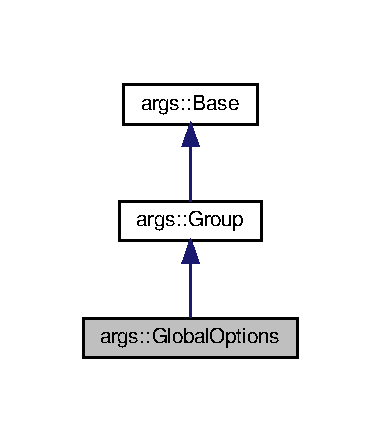
\includegraphics[width=183pt]{classargs_1_1_global_options__inherit__graph}
\end{center}
\end{figure}


Collaboration diagram for args\+:\+:Global\+Options\+:\nopagebreak
\begin{figure}[H]
\begin{center}
\leavevmode
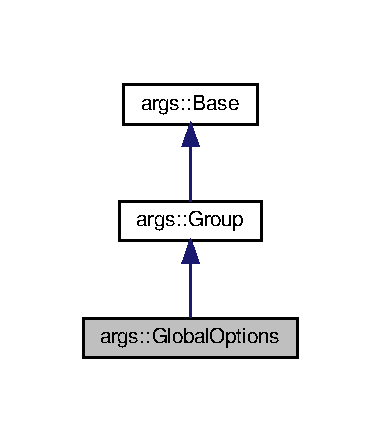
\includegraphics[width=183pt]{classargs_1_1_global_options__coll__graph}
\end{center}
\end{figure}
\subsection*{Public Member Functions}
\begin{DoxyCompactItemize}
\item 
\hyperlink{classargs_1_1_global_options_abbf234c39d3f2a7ece77e006d03e8c52}{Global\+Options} (\hyperlink{classargs_1_1_group}{Group} \&base, \hyperlink{classargs_1_1_base}{Base} \&options\+\_\+)
\end{DoxyCompactItemize}
\subsection*{Additional Inherited Members}


\subsection{Detailed Description}
Class for using global options in \hyperlink{classargs_1_1_argument_parser}{Argument\+Parser}. 

\subsection{Constructor \& Destructor Documentation}
\mbox{\Hypertarget{classargs_1_1_global_options_abbf234c39d3f2a7ece77e006d03e8c52}\label{classargs_1_1_global_options_abbf234c39d3f2a7ece77e006d03e8c52}} 
\index{args\+::\+Global\+Options@{args\+::\+Global\+Options}!Global\+Options@{Global\+Options}}
\index{Global\+Options@{Global\+Options}!args\+::\+Global\+Options@{args\+::\+Global\+Options}}
\subsubsection{\texorpdfstring{Global\+Options()}{GlobalOptions()}}
{\footnotesize\ttfamily args\+::\+Global\+Options\+::\+Global\+Options (\begin{DoxyParamCaption}\item[{\hyperlink{classargs_1_1_group}{Group} \&}]{base,  }\item[{\hyperlink{classargs_1_1_base}{Base} \&}]{options\+\_\+ }\end{DoxyParamCaption})\hspace{0.3cm}{\ttfamily [inline]}}



The documentation for this class was generated from the following file\+:\begin{DoxyCompactItemize}
\item 
/home/cappelletto/github/self/landing\+\_\+area\+\_\+detector/external/\hyperlink{args_8hxx}{args.\+hxx}\end{DoxyCompactItemize}

\hypertarget{classargs_1_1_group}{}\section{args\+:\+:Group Class Reference}
\label{classargs_1_1_group}\index{args\+::\+Group@{args\+::\+Group}}


{\ttfamily \#include $<$args.\+hxx$>$}



Inheritance diagram for args\+:\+:Group\+:\nopagebreak
\begin{figure}[H]
\begin{center}
\leavevmode
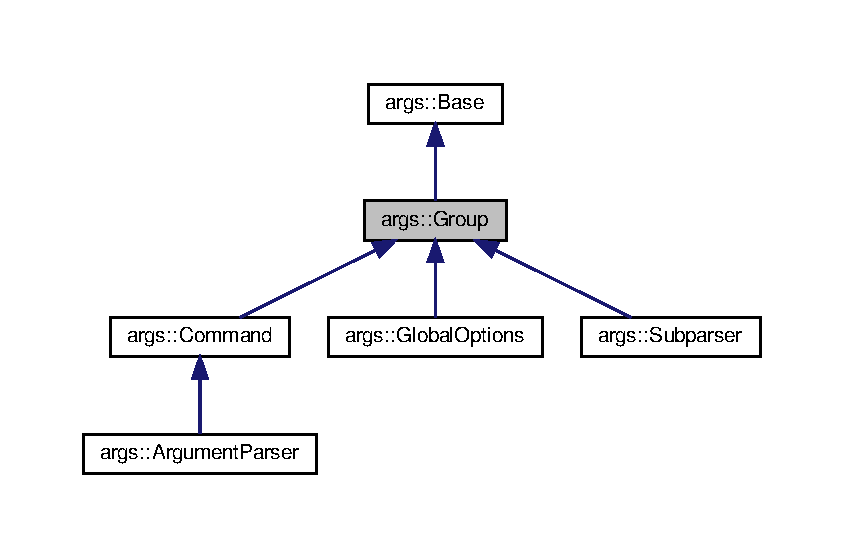
\includegraphics[width=350pt]{classargs_1_1_group__inherit__graph}
\end{center}
\end{figure}


Collaboration diagram for args\+:\+:Group\+:\nopagebreak
\begin{figure}[H]
\begin{center}
\leavevmode
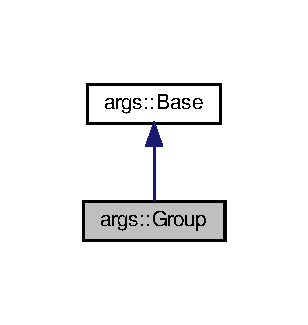
\includegraphics[width=148pt]{classargs_1_1_group__coll__graph}
\end{center}
\end{figure}
\subsection*{Classes}
\begin{DoxyCompactItemize}
\item 
struct \hyperlink{structargs_1_1_group_1_1_validators}{Validators}
\end{DoxyCompactItemize}
\subsection*{Public Member Functions}
\begin{DoxyCompactItemize}
\item 
\hyperlink{classargs_1_1_group_a7474f489d5452569131406185951c64f}{Group} (const std\+::string \&help\+\_\+=std\+::string(), const std\+::function$<$ bool(const \hyperlink{classargs_1_1_group}{Group} \&)$>$ \&validator\+\_\+=\hyperlink{structargs_1_1_group_1_1_validators_adf7a904f8fa0d4ea9f1c47ea057a5417}{Validators\+::\+Dont\+Care}, \hyperlink{namespaceargs_aa530c0f95194aa275f49a5f299ac9e77}{Options} options\+\_\+=\{\})
\begin{DoxyCompactList}\small\item\em If help is empty, this group will not be printed in help output. \end{DoxyCompactList}\item 
\hyperlink{classargs_1_1_group_a54598c07578eac848838a21e4dd98657}{Group} (\hyperlink{classargs_1_1_group}{Group} \&group\+\_\+, const std\+::string \&help\+\_\+=std\+::string(), const std\+::function$<$ bool(const \hyperlink{classargs_1_1_group}{Group} \&)$>$ \&validator\+\_\+=\hyperlink{structargs_1_1_group_1_1_validators_adf7a904f8fa0d4ea9f1c47ea057a5417}{Validators\+::\+Dont\+Care}, \hyperlink{namespaceargs_aa530c0f95194aa275f49a5f299ac9e77}{Options} options\+\_\+=\{\})
\begin{DoxyCompactList}\small\item\em If help is empty, this group will not be printed in help output. \end{DoxyCompactList}\item 
virtual \hyperlink{classargs_1_1_group_a928331572568f1d3878f870323da8024}{$\sim$\+Group} ()
\item 
void \hyperlink{classargs_1_1_group_ae5951da80c2ca072299740021c43bf6b}{Add} (\hyperlink{classargs_1_1_base}{Base} \&child)
\item 
const std\+::vector$<$ \hyperlink{classargs_1_1_base}{Base} $\ast$ $>$ \& \hyperlink{classargs_1_1_group_ad78496495550a3b9a9f92468513905ae}{Children} () const
\item 
virtual \hyperlink{classargs_1_1_flag_base}{Flag\+Base} $\ast$ \hyperlink{classargs_1_1_group_a31872f412d5b32e0afaf962cd2ce5e40}{Match} (const \hyperlink{structargs_1_1_either_flag}{Either\+Flag} \&flag) override
\item 
virtual void \hyperlink{classargs_1_1_group_a9f74bb3d58e5bfe331a6af8a9981ebda}{Validate} (const std\+::string \&short\+Prefix, const std\+::string \&long\+Prefix) const override
\item 
virtual \hyperlink{classargs_1_1_positional_base}{Positional\+Base} $\ast$ \hyperlink{classargs_1_1_group_ae0fa8f5ae77fda45086e7815617ddff7}{Get\+Next\+Positional} () override
\item 
virtual bool \hyperlink{classargs_1_1_group_a67e35305748038c175dee92ad1f5290f}{Has\+Flag} () const override
\item 
virtual bool \hyperlink{classargs_1_1_group_a3d976f35f65ed8e4908eb88ce84accd4}{Has\+Positional} () const override
\item 
virtual bool \hyperlink{classargs_1_1_group_a022cbdf1f4bfe4210a56fa8ca9045bf8}{Has\+Command} () const override
\item 
std\+::vector$<$ \hyperlink{classargs_1_1_base}{Base} $\ast$ $>$\+::size\+\_\+type \hyperlink{classargs_1_1_group_a63697db6c1a28632775f852afface1ce}{Matched\+Children} () const
\item 
virtual bool \hyperlink{classargs_1_1_group_a7794d31edae97254be440b8768db9af0}{Matched} () const noexcept override
\item 
bool \hyperlink{classargs_1_1_group_ad95fc2e1615bd75cdffdad82daa67df4}{Get} () const
\item 
virtual std\+::vector$<$ std\+::tuple$<$ std\+::string, std\+::string, unsigned $>$ $>$ \hyperlink{classargs_1_1_group_a57068f355d7d62316b41f7a8e2528495}{Get\+Description} (const \hyperlink{structargs_1_1_help_params}{Help\+Params} \&params, const unsigned int indent) const override
\item 
virtual std\+::vector$<$ std\+::string $>$ \hyperlink{classargs_1_1_group_abe9ab07499ec19e941df8f38e18089df}{Get\+Program\+Line} (const \hyperlink{structargs_1_1_help_params}{Help\+Params} \&params) const override
\item 
virtual std\+::vector$<$ \hyperlink{classargs_1_1_command}{Command} $\ast$ $>$ \hyperlink{classargs_1_1_group_a83b0a40e16d92c0f387d00a0f35dbf17}{Get\+Commands} () override
\item 
virtual bool \hyperlink{classargs_1_1_group_a60de0a1db5be506a8638af0d3ce329bc}{Is\+Group} () const override
\item 
virtual void \hyperlink{classargs_1_1_group_a7ccee0f0ea0902b82029b2ab30f3f84b}{Reset} () noexcept override
\end{DoxyCompactItemize}
\subsection*{Additional Inherited Members}


\subsection{Detailed Description}
Class for all kinds of validating groups, including \hyperlink{classargs_1_1_argument_parser}{Argument\+Parser} 

\subsection{Constructor \& Destructor Documentation}
\mbox{\Hypertarget{classargs_1_1_group_a7474f489d5452569131406185951c64f}\label{classargs_1_1_group_a7474f489d5452569131406185951c64f}} 
\index{args\+::\+Group@{args\+::\+Group}!Group@{Group}}
\index{Group@{Group}!args\+::\+Group@{args\+::\+Group}}
\subsubsection{\texorpdfstring{Group()}{Group()}\hspace{0.1cm}{\footnotesize\ttfamily [1/2]}}
{\footnotesize\ttfamily args\+::\+Group\+::\+Group (\begin{DoxyParamCaption}\item[{const std\+::string \&}]{help\+\_\+ = {\ttfamily std\+:\+:string()},  }\item[{const std\+::function$<$ bool(const \hyperlink{classargs_1_1_group}{Group} \&)$>$ \&}]{validator\+\_\+ = {\ttfamily \hyperlink{structargs_1_1_group_1_1_validators_adf7a904f8fa0d4ea9f1c47ea057a5417}{Validators\+::\+Dont\+Care}},  }\item[{\hyperlink{namespaceargs_aa530c0f95194aa275f49a5f299ac9e77}{Options}}]{options\+\_\+ = {\ttfamily \{\}} }\end{DoxyParamCaption})\hspace{0.3cm}{\ttfamily [inline]}}



If help is empty, this group will not be printed in help output. 

\mbox{\Hypertarget{classargs_1_1_group_a54598c07578eac848838a21e4dd98657}\label{classargs_1_1_group_a54598c07578eac848838a21e4dd98657}} 
\index{args\+::\+Group@{args\+::\+Group}!Group@{Group}}
\index{Group@{Group}!args\+::\+Group@{args\+::\+Group}}
\subsubsection{\texorpdfstring{Group()}{Group()}\hspace{0.1cm}{\footnotesize\ttfamily [2/2]}}
{\footnotesize\ttfamily args\+::\+Group\+::\+Group (\begin{DoxyParamCaption}\item[{\hyperlink{classargs_1_1_group}{Group} \&}]{group\+\_\+,  }\item[{const std\+::string \&}]{help\+\_\+ = {\ttfamily std\+:\+:string()},  }\item[{const std\+::function$<$ bool(const \hyperlink{classargs_1_1_group}{Group} \&)$>$ \&}]{validator\+\_\+ = {\ttfamily \hyperlink{structargs_1_1_group_1_1_validators_adf7a904f8fa0d4ea9f1c47ea057a5417}{Validators\+::\+Dont\+Care}},  }\item[{\hyperlink{namespaceargs_aa530c0f95194aa275f49a5f299ac9e77}{Options}}]{options\+\_\+ = {\ttfamily \{\}} }\end{DoxyParamCaption})\hspace{0.3cm}{\ttfamily [inline]}}



If help is empty, this group will not be printed in help output. 

\mbox{\Hypertarget{classargs_1_1_group_a928331572568f1d3878f870323da8024}\label{classargs_1_1_group_a928331572568f1d3878f870323da8024}} 
\index{args\+::\+Group@{args\+::\+Group}!````~Group@{$\sim$\+Group}}
\index{````~Group@{$\sim$\+Group}!args\+::\+Group@{args\+::\+Group}}
\subsubsection{\texorpdfstring{$\sim$\+Group()}{~Group()}}
{\footnotesize\ttfamily virtual args\+::\+Group\+::$\sim$\+Group (\begin{DoxyParamCaption}{ }\end{DoxyParamCaption})\hspace{0.3cm}{\ttfamily [inline]}, {\ttfamily [virtual]}}



\subsection{Member Function Documentation}
\mbox{\Hypertarget{classargs_1_1_group_ae5951da80c2ca072299740021c43bf6b}\label{classargs_1_1_group_ae5951da80c2ca072299740021c43bf6b}} 
\index{args\+::\+Group@{args\+::\+Group}!Add@{Add}}
\index{Add@{Add}!args\+::\+Group@{args\+::\+Group}}
\subsubsection{\texorpdfstring{Add()}{Add()}}
{\footnotesize\ttfamily void args\+::\+Group\+::\+Add (\begin{DoxyParamCaption}\item[{\hyperlink{classargs_1_1_base}{Base} \&}]{child }\end{DoxyParamCaption})\hspace{0.3cm}{\ttfamily [inline]}}

Append a child to this \hyperlink{classargs_1_1_group}{Group}. \mbox{\Hypertarget{classargs_1_1_group_ad78496495550a3b9a9f92468513905ae}\label{classargs_1_1_group_ad78496495550a3b9a9f92468513905ae}} 
\index{args\+::\+Group@{args\+::\+Group}!Children@{Children}}
\index{Children@{Children}!args\+::\+Group@{args\+::\+Group}}
\subsubsection{\texorpdfstring{Children()}{Children()}}
{\footnotesize\ttfamily const std\+::vector$<$\hyperlink{classargs_1_1_base}{Base} $\ast$$>$\& args\+::\+Group\+::\+Children (\begin{DoxyParamCaption}{ }\end{DoxyParamCaption}) const\hspace{0.3cm}{\ttfamily [inline]}}

Get all this group\textquotesingle{}s children \mbox{\Hypertarget{classargs_1_1_group_ad95fc2e1615bd75cdffdad82daa67df4}\label{classargs_1_1_group_ad95fc2e1615bd75cdffdad82daa67df4}} 
\index{args\+::\+Group@{args\+::\+Group}!Get@{Get}}
\index{Get@{Get}!args\+::\+Group@{args\+::\+Group}}
\subsubsection{\texorpdfstring{Get()}{Get()}}
{\footnotesize\ttfamily bool args\+::\+Group\+::\+Get (\begin{DoxyParamCaption}{ }\end{DoxyParamCaption}) const\hspace{0.3cm}{\ttfamily [inline]}}

Get validation \mbox{\Hypertarget{classargs_1_1_group_a83b0a40e16d92c0f387d00a0f35dbf17}\label{classargs_1_1_group_a83b0a40e16d92c0f387d00a0f35dbf17}} 
\index{args\+::\+Group@{args\+::\+Group}!Get\+Commands@{Get\+Commands}}
\index{Get\+Commands@{Get\+Commands}!args\+::\+Group@{args\+::\+Group}}
\subsubsection{\texorpdfstring{Get\+Commands()}{GetCommands()}}
{\footnotesize\ttfamily virtual std\+::vector$<$\hyperlink{classargs_1_1_command}{Command}$\ast$$>$ args\+::\+Group\+::\+Get\+Commands (\begin{DoxyParamCaption}{ }\end{DoxyParamCaption})\hspace{0.3cm}{\ttfamily [inline]}, {\ttfamily [override]}, {\ttfamily [virtual]}}



Reimplemented from \hyperlink{classargs_1_1_base_a8b41df1247be5545f95279608d835bf2}{args\+::\+Base}.



Reimplemented in \hyperlink{classargs_1_1_command_a59511be164aa3a0cc5fbbfb75ca79fec}{args\+::\+Command}.

\mbox{\Hypertarget{classargs_1_1_group_a57068f355d7d62316b41f7a8e2528495}\label{classargs_1_1_group_a57068f355d7d62316b41f7a8e2528495}} 
\index{args\+::\+Group@{args\+::\+Group}!Get\+Description@{Get\+Description}}
\index{Get\+Description@{Get\+Description}!args\+::\+Group@{args\+::\+Group}}
\subsubsection{\texorpdfstring{Get\+Description()}{GetDescription()}}
{\footnotesize\ttfamily virtual std\+::vector$<$std\+::tuple$<$std\+::string, std\+::string, unsigned$>$ $>$ args\+::\+Group\+::\+Get\+Description (\begin{DoxyParamCaption}\item[{const \hyperlink{structargs_1_1_help_params}{Help\+Params} \&}]{params,  }\item[{const unsigned int}]{indent }\end{DoxyParamCaption}) const\hspace{0.3cm}{\ttfamily [inline]}, {\ttfamily [override]}, {\ttfamily [virtual]}}

Get all the child descriptions for help generation 

Reimplemented in \hyperlink{classargs_1_1_command_afdd0a3ea344a4a5672565d1f2f0157f1}{args\+::\+Command}.

\mbox{\Hypertarget{classargs_1_1_group_ae0fa8f5ae77fda45086e7815617ddff7}\label{classargs_1_1_group_ae0fa8f5ae77fda45086e7815617ddff7}} 
\index{args\+::\+Group@{args\+::\+Group}!Get\+Next\+Positional@{Get\+Next\+Positional}}
\index{Get\+Next\+Positional@{Get\+Next\+Positional}!args\+::\+Group@{args\+::\+Group}}
\subsubsection{\texorpdfstring{Get\+Next\+Positional()}{GetNextPositional()}}
{\footnotesize\ttfamily virtual \hyperlink{classargs_1_1_positional_base}{Positional\+Base}$\ast$ args\+::\+Group\+::\+Get\+Next\+Positional (\begin{DoxyParamCaption}{ }\end{DoxyParamCaption})\hspace{0.3cm}{\ttfamily [inline]}, {\ttfamily [override]}, {\ttfamily [virtual]}}

Get the next ready positional, or nullptr if there is none

\begin{DoxyReturn}{Returns}
the first ready \hyperlink{classargs_1_1_positional_base}{Positional\+Base} pointer, or nullptr if there is no match 
\end{DoxyReturn}


Reimplemented from \hyperlink{classargs_1_1_base_a3e5ad8516fd2037496cd39bcb3b10f9d}{args\+::\+Base}.



Reimplemented in \hyperlink{classargs_1_1_command_a073266d188b3592f745c64567e566f8a}{args\+::\+Command}.

\mbox{\Hypertarget{classargs_1_1_group_abe9ab07499ec19e941df8f38e18089df}\label{classargs_1_1_group_abe9ab07499ec19e941df8f38e18089df}} 
\index{args\+::\+Group@{args\+::\+Group}!Get\+Program\+Line@{Get\+Program\+Line}}
\index{Get\+Program\+Line@{Get\+Program\+Line}!args\+::\+Group@{args\+::\+Group}}
\subsubsection{\texorpdfstring{Get\+Program\+Line()}{GetProgramLine()}}
{\footnotesize\ttfamily virtual std\+::vector$<$std\+::string$>$ args\+::\+Group\+::\+Get\+Program\+Line (\begin{DoxyParamCaption}\item[{const \hyperlink{structargs_1_1_help_params}{Help\+Params} \&}]{params }\end{DoxyParamCaption}) const\hspace{0.3cm}{\ttfamily [inline]}, {\ttfamily [override]}, {\ttfamily [virtual]}}

Get the names of positional parameters 

Reimplemented from \hyperlink{classargs_1_1_base_a88fcbbc4bfe3b7af9fafe6e96a19f337}{args\+::\+Base}.



Reimplemented in \hyperlink{classargs_1_1_command_a37fbbde216ce232279e04edce12c1245}{args\+::\+Command}.

\mbox{\Hypertarget{classargs_1_1_group_a022cbdf1f4bfe4210a56fa8ca9045bf8}\label{classargs_1_1_group_a022cbdf1f4bfe4210a56fa8ca9045bf8}} 
\index{args\+::\+Group@{args\+::\+Group}!Has\+Command@{Has\+Command}}
\index{Has\+Command@{Has\+Command}!args\+::\+Group@{args\+::\+Group}}
\subsubsection{\texorpdfstring{Has\+Command()}{HasCommand()}}
{\footnotesize\ttfamily virtual bool args\+::\+Group\+::\+Has\+Command (\begin{DoxyParamCaption}{ }\end{DoxyParamCaption}) const\hspace{0.3cm}{\ttfamily [inline]}, {\ttfamily [override]}, {\ttfamily [virtual]}}

Get whether this has any \hyperlink{classargs_1_1_command}{Command} children

\begin{DoxyReturn}{Returns}
Whether or not there are any \hyperlink{classargs_1_1_command}{Command} children 
\end{DoxyReturn}


Reimplemented from \hyperlink{classargs_1_1_base_a78322109f31edba4bb467d73e6663422}{args\+::\+Base}.



Reimplemented in \hyperlink{classargs_1_1_command_aa7117d38f553f127542434f6cafc2697}{args\+::\+Command}.

\mbox{\Hypertarget{classargs_1_1_group_a67e35305748038c175dee92ad1f5290f}\label{classargs_1_1_group_a67e35305748038c175dee92ad1f5290f}} 
\index{args\+::\+Group@{args\+::\+Group}!Has\+Flag@{Has\+Flag}}
\index{Has\+Flag@{Has\+Flag}!args\+::\+Group@{args\+::\+Group}}
\subsubsection{\texorpdfstring{Has\+Flag()}{HasFlag()}}
{\footnotesize\ttfamily virtual bool args\+::\+Group\+::\+Has\+Flag (\begin{DoxyParamCaption}{ }\end{DoxyParamCaption}) const\hspace{0.3cm}{\ttfamily [inline]}, {\ttfamily [override]}, {\ttfamily [virtual]}}

Get whether this has any \hyperlink{classargs_1_1_flag_base}{Flag\+Base} children

\begin{DoxyReturn}{Returns}
Whether or not there are any \hyperlink{classargs_1_1_flag_base}{Flag\+Base} children 
\end{DoxyReturn}


Reimplemented from \hyperlink{classargs_1_1_base_a81684f399665c0372439c070af5de4a7}{args\+::\+Base}.



Reimplemented in \hyperlink{classargs_1_1_command_abcf9fafcb1531d3c0ea8a1b3a31c6ba4}{args\+::\+Command}.

\mbox{\Hypertarget{classargs_1_1_group_a3d976f35f65ed8e4908eb88ce84accd4}\label{classargs_1_1_group_a3d976f35f65ed8e4908eb88ce84accd4}} 
\index{args\+::\+Group@{args\+::\+Group}!Has\+Positional@{Has\+Positional}}
\index{Has\+Positional@{Has\+Positional}!args\+::\+Group@{args\+::\+Group}}
\subsubsection{\texorpdfstring{Has\+Positional()}{HasPositional()}}
{\footnotesize\ttfamily virtual bool args\+::\+Group\+::\+Has\+Positional (\begin{DoxyParamCaption}{ }\end{DoxyParamCaption}) const\hspace{0.3cm}{\ttfamily [inline]}, {\ttfamily [override]}, {\ttfamily [virtual]}}

Get whether this has any \hyperlink{classargs_1_1_positional_base}{Positional\+Base} children

\begin{DoxyReturn}{Returns}
Whether or not there are any \hyperlink{classargs_1_1_positional_base}{Positional\+Base} children 
\end{DoxyReturn}


Reimplemented from \hyperlink{classargs_1_1_base_a3825f4afe867335438103a0d45ced9f7}{args\+::\+Base}.



Reimplemented in \hyperlink{classargs_1_1_command_a5c430c5f36d678e80420d2f094ac3a4d}{args\+::\+Command}.

\mbox{\Hypertarget{classargs_1_1_group_a60de0a1db5be506a8638af0d3ce329bc}\label{classargs_1_1_group_a60de0a1db5be506a8638af0d3ce329bc}} 
\index{args\+::\+Group@{args\+::\+Group}!Is\+Group@{Is\+Group}}
\index{Is\+Group@{Is\+Group}!args\+::\+Group@{args\+::\+Group}}
\subsubsection{\texorpdfstring{Is\+Group()}{IsGroup()}}
{\footnotesize\ttfamily virtual bool args\+::\+Group\+::\+Is\+Group (\begin{DoxyParamCaption}{ }\end{DoxyParamCaption}) const\hspace{0.3cm}{\ttfamily [inline]}, {\ttfamily [override]}, {\ttfamily [virtual]}}



Reimplemented from \hyperlink{classargs_1_1_base_a72e11d38c82b8dca87b830853676b68c}{args\+::\+Base}.



Reimplemented in \hyperlink{classargs_1_1_command_acc75daa42b98b9be35718f072a46f13a}{args\+::\+Command}.

\mbox{\Hypertarget{classargs_1_1_group_a31872f412d5b32e0afaf962cd2ce5e40}\label{classargs_1_1_group_a31872f412d5b32e0afaf962cd2ce5e40}} 
\index{args\+::\+Group@{args\+::\+Group}!Match@{Match}}
\index{Match@{Match}!args\+::\+Group@{args\+::\+Group}}
\subsubsection{\texorpdfstring{Match()}{Match()}}
{\footnotesize\ttfamily virtual \hyperlink{classargs_1_1_flag_base}{Flag\+Base}$\ast$ args\+::\+Group\+::\+Match (\begin{DoxyParamCaption}\item[{const \hyperlink{structargs_1_1_either_flag}{Either\+Flag} \&}]{flag }\end{DoxyParamCaption})\hspace{0.3cm}{\ttfamily [inline]}, {\ttfamily [override]}, {\ttfamily [virtual]}}

Return the first \hyperlink{classargs_1_1_flag_base}{Flag\+Base} that matches flag, or nullptr


\begin{DoxyParams}{Parameters}
{\em flag} & The flag with prefixes stripped \\
\hline
\end{DoxyParams}
\begin{DoxyReturn}{Returns}
the first matching \hyperlink{classargs_1_1_flag_base}{Flag\+Base} pointer, or nullptr if there is no match 
\end{DoxyReturn}


Reimplemented from \hyperlink{classargs_1_1_base_a6d5a7be35d62f59fee5a52c06af3003e}{args\+::\+Base}.



Reimplemented in \hyperlink{classargs_1_1_command_ace018e92977b0e6ec5472cae0166523c}{args\+::\+Command}.

\mbox{\Hypertarget{classargs_1_1_group_a7794d31edae97254be440b8768db9af0}\label{classargs_1_1_group_a7794d31edae97254be440b8768db9af0}} 
\index{args\+::\+Group@{args\+::\+Group}!Matched@{Matched}}
\index{Matched@{Matched}!args\+::\+Group@{args\+::\+Group}}
\subsubsection{\texorpdfstring{Matched()}{Matched()}}
{\footnotesize\ttfamily virtual bool args\+::\+Group\+::\+Matched (\begin{DoxyParamCaption}{ }\end{DoxyParamCaption}) const\hspace{0.3cm}{\ttfamily [inline]}, {\ttfamily [override]}, {\ttfamily [virtual]}, {\ttfamily [noexcept]}}

Whether or not this group matches validation 

Reimplemented from \hyperlink{classargs_1_1_base_ae7ae4ca8ad953be1a353991c1df6ec4d}{args\+::\+Base}.



Reimplemented in \hyperlink{classargs_1_1_command_aebb9c512301e7f0c49689ed92568ef6e}{args\+::\+Command}.

\mbox{\Hypertarget{classargs_1_1_group_a63697db6c1a28632775f852afface1ce}\label{classargs_1_1_group_a63697db6c1a28632775f852afface1ce}} 
\index{args\+::\+Group@{args\+::\+Group}!Matched\+Children@{Matched\+Children}}
\index{Matched\+Children@{Matched\+Children}!args\+::\+Group@{args\+::\+Group}}
\subsubsection{\texorpdfstring{Matched\+Children()}{MatchedChildren()}}
{\footnotesize\ttfamily std\+::vector$<$\hyperlink{classargs_1_1_base}{Base} $\ast$$>$\+::size\+\_\+type args\+::\+Group\+::\+Matched\+Children (\begin{DoxyParamCaption}{ }\end{DoxyParamCaption}) const\hspace{0.3cm}{\ttfamily [inline]}}

Count the number of matched children this group has \mbox{\Hypertarget{classargs_1_1_group_a7ccee0f0ea0902b82029b2ab30f3f84b}\label{classargs_1_1_group_a7ccee0f0ea0902b82029b2ab30f3f84b}} 
\index{args\+::\+Group@{args\+::\+Group}!Reset@{Reset}}
\index{Reset@{Reset}!args\+::\+Group@{args\+::\+Group}}
\subsubsection{\texorpdfstring{Reset()}{Reset()}}
{\footnotesize\ttfamily virtual void args\+::\+Group\+::\+Reset (\begin{DoxyParamCaption}{ }\end{DoxyParamCaption})\hspace{0.3cm}{\ttfamily [inline]}, {\ttfamily [override]}, {\ttfamily [virtual]}, {\ttfamily [noexcept]}}



Reimplemented from \hyperlink{classargs_1_1_base_ac7cfc851174f71e00173121d3013dab1}{args\+::\+Base}.



Reimplemented in \hyperlink{classargs_1_1_argument_parser_a73b0dc7bc87c3a44345879f34985237f}{args\+::\+Argument\+Parser}, and \hyperlink{classargs_1_1_command_aa1829501dd4f63ba3551bf85171be83e}{args\+::\+Command}.

\mbox{\Hypertarget{classargs_1_1_group_a9f74bb3d58e5bfe331a6af8a9981ebda}\label{classargs_1_1_group_a9f74bb3d58e5bfe331a6af8a9981ebda}} 
\index{args\+::\+Group@{args\+::\+Group}!Validate@{Validate}}
\index{Validate@{Validate}!args\+::\+Group@{args\+::\+Group}}
\subsubsection{\texorpdfstring{Validate()}{Validate()}}
{\footnotesize\ttfamily virtual void args\+::\+Group\+::\+Validate (\begin{DoxyParamCaption}\item[{const std\+::string \&}]{short\+Prefix,  }\item[{const std\+::string \&}]{long\+Prefix }\end{DoxyParamCaption}) const\hspace{0.3cm}{\ttfamily [inline]}, {\ttfamily [override]}, {\ttfamily [virtual]}}



Reimplemented from \hyperlink{classargs_1_1_base_a62ea917978306062785cbfaa4dd51d2f}{args\+::\+Base}.



Reimplemented in \hyperlink{classargs_1_1_command_ad39b397a91af426f0ecbda9d29d7bbe0}{args\+::\+Command}.



The documentation for this class was generated from the following file\+:\begin{DoxyCompactItemize}
\item 
/home/cappelletto/github/self/landing\+\_\+area\+\_\+detector/external/\hyperlink{args_8hxx}{args.\+hxx}\end{DoxyCompactItemize}

\hypertarget{classargs_1_1_help}{}\section{args\+:\+:Help Class Reference}
\label{classargs_1_1_help}\index{args\+::\+Help@{args\+::\+Help}}


{\ttfamily \#include $<$args.\+hxx$>$}



Inheritance diagram for args\+:\+:Help\+:\nopagebreak
\begin{figure}[H]
\begin{center}
\leavevmode
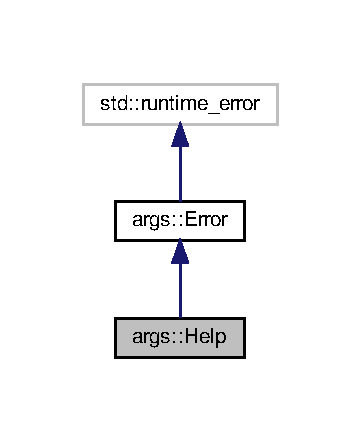
\includegraphics[width=173pt]{classargs_1_1_help__inherit__graph}
\end{center}
\end{figure}


Collaboration diagram for args\+:\+:Help\+:\nopagebreak
\begin{figure}[H]
\begin{center}
\leavevmode
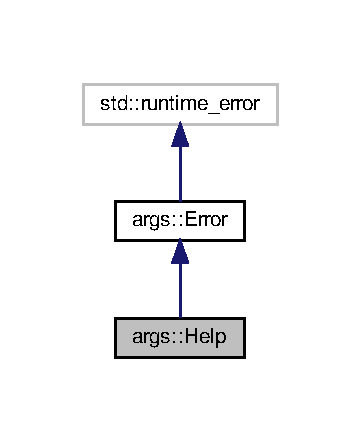
\includegraphics[width=173pt]{classargs_1_1_help__coll__graph}
\end{center}
\end{figure}
\subsection*{Public Member Functions}
\begin{DoxyCompactItemize}
\item 
\hyperlink{classargs_1_1_help_a48a25063191a6792bd1582884b940d01}{Help} (const std\+::string \&flag)
\item 
virtual \hyperlink{classargs_1_1_help_abf8f1186f2b1d38cb457e8a589182ec1}{$\sim$\+Help} ()
\end{DoxyCompactItemize}


\subsection{Detailed Description}
An exception that indicates that the user has requested help 

\subsection{Constructor \& Destructor Documentation}
\mbox{\Hypertarget{classargs_1_1_help_a48a25063191a6792bd1582884b940d01}\label{classargs_1_1_help_a48a25063191a6792bd1582884b940d01}} 
\index{args\+::\+Help@{args\+::\+Help}!Help@{Help}}
\index{Help@{Help}!args\+::\+Help@{args\+::\+Help}}
\subsubsection{\texorpdfstring{Help()}{Help()}}
{\footnotesize\ttfamily args\+::\+Help\+::\+Help (\begin{DoxyParamCaption}\item[{const std\+::string \&}]{flag }\end{DoxyParamCaption})\hspace{0.3cm}{\ttfamily [inline]}}

\mbox{\Hypertarget{classargs_1_1_help_abf8f1186f2b1d38cb457e8a589182ec1}\label{classargs_1_1_help_abf8f1186f2b1d38cb457e8a589182ec1}} 
\index{args\+::\+Help@{args\+::\+Help}!````~Help@{$\sim$\+Help}}
\index{````~Help@{$\sim$\+Help}!args\+::\+Help@{args\+::\+Help}}
\subsubsection{\texorpdfstring{$\sim$\+Help()}{~Help()}}
{\footnotesize\ttfamily virtual args\+::\+Help\+::$\sim$\+Help (\begin{DoxyParamCaption}{ }\end{DoxyParamCaption})\hspace{0.3cm}{\ttfamily [inline]}, {\ttfamily [virtual]}}



The documentation for this class was generated from the following file\+:\begin{DoxyCompactItemize}
\item 
/home/cappelletto/github/self/landing\+\_\+area\+\_\+detector/external/\hyperlink{args_8hxx}{args.\+hxx}\end{DoxyCompactItemize}

\hypertarget{classargs_1_1_help_flag}{}\section{args\+:\+:Help\+Flag Class Reference}
\label{classargs_1_1_help_flag}\index{args\+::\+Help\+Flag@{args\+::\+Help\+Flag}}


{\ttfamily \#include $<$args.\+hxx$>$}



Inheritance diagram for args\+:\+:Help\+Flag\+:\nopagebreak
\begin{figure}[H]
\begin{center}
\leavevmode
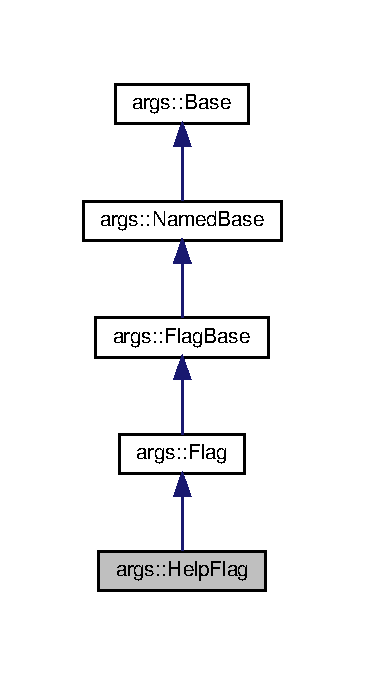
\includegraphics[width=175pt]{classargs_1_1_help_flag__inherit__graph}
\end{center}
\end{figure}


Collaboration diagram for args\+:\+:Help\+Flag\+:\nopagebreak
\begin{figure}[H]
\begin{center}
\leavevmode
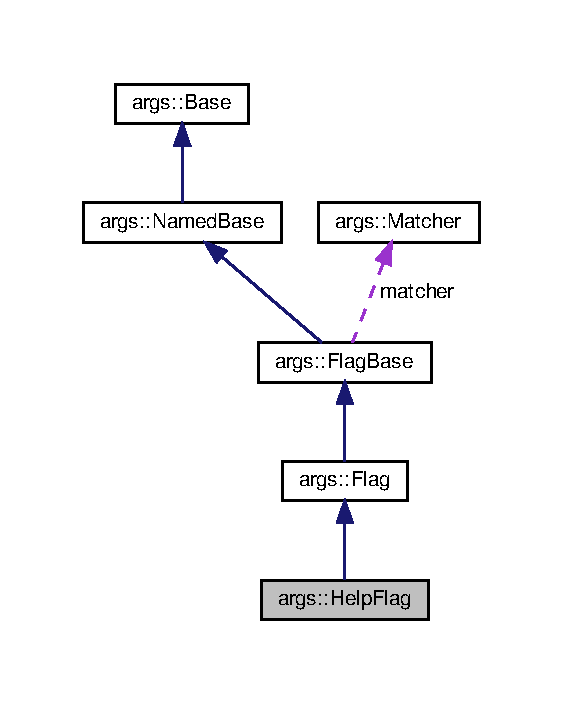
\includegraphics[width=270pt]{classargs_1_1_help_flag__coll__graph}
\end{center}
\end{figure}
\subsection*{Public Member Functions}
\begin{DoxyCompactItemize}
\item 
\hyperlink{classargs_1_1_help_flag_a6ee9c6725d5ce9d57090e2aab59cb050}{Help\+Flag} (\hyperlink{classargs_1_1_group}{Group} \&group\+\_\+, const std\+::string \&name\+\_\+, const std\+::string \&help\+\_\+, \hyperlink{classargs_1_1_matcher}{Matcher} \&\&matcher\+\_\+, \hyperlink{namespaceargs_aa530c0f95194aa275f49a5f299ac9e77}{Options} options\+\_\+=\{\})
\item 
virtual \hyperlink{classargs_1_1_help_flag_acd28f5106f158d7da9aace1ea55bea63}{$\sim$\+Help\+Flag} ()
\item 
virtual \hyperlink{classargs_1_1_flag_base}{Flag\+Base} $\ast$ \hyperlink{classargs_1_1_help_flag_a1a555992a7c8350aca0ac1f292d91605}{Match} (const \hyperlink{structargs_1_1_either_flag}{Either\+Flag} \&arg) override
\item 
bool \hyperlink{classargs_1_1_help_flag_a4a7d60a403961377da9cf9203f7b4203}{Get} () const noexcept
\end{DoxyCompactItemize}
\subsection*{Additional Inherited Members}


\subsection{Detailed Description}
\hyperlink{classargs_1_1_help}{Help} flag class

Works like a regular flag, but throws an instance of \hyperlink{classargs_1_1_help}{Help} when it is matched 

\subsection{Constructor \& Destructor Documentation}
\mbox{\Hypertarget{classargs_1_1_help_flag_a6ee9c6725d5ce9d57090e2aab59cb050}\label{classargs_1_1_help_flag_a6ee9c6725d5ce9d57090e2aab59cb050}} 
\index{args\+::\+Help\+Flag@{args\+::\+Help\+Flag}!Help\+Flag@{Help\+Flag}}
\index{Help\+Flag@{Help\+Flag}!args\+::\+Help\+Flag@{args\+::\+Help\+Flag}}
\subsubsection{\texorpdfstring{Help\+Flag()}{HelpFlag()}}
{\footnotesize\ttfamily args\+::\+Help\+Flag\+::\+Help\+Flag (\begin{DoxyParamCaption}\item[{\hyperlink{classargs_1_1_group}{Group} \&}]{group\+\_\+,  }\item[{const std\+::string \&}]{name\+\_\+,  }\item[{const std\+::string \&}]{help\+\_\+,  }\item[{\hyperlink{classargs_1_1_matcher}{Matcher} \&\&}]{matcher\+\_\+,  }\item[{\hyperlink{namespaceargs_aa530c0f95194aa275f49a5f299ac9e77}{Options}}]{options\+\_\+ = {\ttfamily \{\}} }\end{DoxyParamCaption})\hspace{0.3cm}{\ttfamily [inline]}}

\mbox{\Hypertarget{classargs_1_1_help_flag_acd28f5106f158d7da9aace1ea55bea63}\label{classargs_1_1_help_flag_acd28f5106f158d7da9aace1ea55bea63}} 
\index{args\+::\+Help\+Flag@{args\+::\+Help\+Flag}!````~Help\+Flag@{$\sim$\+Help\+Flag}}
\index{````~Help\+Flag@{$\sim$\+Help\+Flag}!args\+::\+Help\+Flag@{args\+::\+Help\+Flag}}
\subsubsection{\texorpdfstring{$\sim$\+Help\+Flag()}{~HelpFlag()}}
{\footnotesize\ttfamily virtual args\+::\+Help\+Flag\+::$\sim$\+Help\+Flag (\begin{DoxyParamCaption}{ }\end{DoxyParamCaption})\hspace{0.3cm}{\ttfamily [inline]}, {\ttfamily [virtual]}}



\subsection{Member Function Documentation}
\mbox{\Hypertarget{classargs_1_1_help_flag_a4a7d60a403961377da9cf9203f7b4203}\label{classargs_1_1_help_flag_a4a7d60a403961377da9cf9203f7b4203}} 
\index{args\+::\+Help\+Flag@{args\+::\+Help\+Flag}!Get@{Get}}
\index{Get@{Get}!args\+::\+Help\+Flag@{args\+::\+Help\+Flag}}
\subsubsection{\texorpdfstring{Get()}{Get()}}
{\footnotesize\ttfamily bool args\+::\+Help\+Flag\+::\+Get (\begin{DoxyParamCaption}{ }\end{DoxyParamCaption}) const\hspace{0.3cm}{\ttfamily [inline]}, {\ttfamily [noexcept]}}

Get whether this was matched \mbox{\Hypertarget{classargs_1_1_help_flag_a1a555992a7c8350aca0ac1f292d91605}\label{classargs_1_1_help_flag_a1a555992a7c8350aca0ac1f292d91605}} 
\index{args\+::\+Help\+Flag@{args\+::\+Help\+Flag}!Match@{Match}}
\index{Match@{Match}!args\+::\+Help\+Flag@{args\+::\+Help\+Flag}}
\subsubsection{\texorpdfstring{Match()}{Match()}}
{\footnotesize\ttfamily virtual \hyperlink{classargs_1_1_flag_base}{Flag\+Base}$\ast$ args\+::\+Help\+Flag\+::\+Match (\begin{DoxyParamCaption}\item[{const \hyperlink{structargs_1_1_either_flag}{Either\+Flag} \&}]{arg }\end{DoxyParamCaption})\hspace{0.3cm}{\ttfamily [inline]}, {\ttfamily [override]}, {\ttfamily [virtual]}}



Reimplemented from \hyperlink{classargs_1_1_flag_base_a729ebb681d373f09875abb2e04f820f2}{args\+::\+Flag\+Base}.



The documentation for this class was generated from the following file\+:\begin{DoxyCompactItemize}
\item 
/home/cappelletto/github/self/landing\+\_\+area\+\_\+detector/external/\hyperlink{args_8hxx}{args.\+hxx}\end{DoxyCompactItemize}

\hypertarget{structargs_1_1_help_params}{}\section{args\+:\+:Help\+Params Struct Reference}
\label{structargs_1_1_help_params}\index{args\+::\+Help\+Params@{args\+::\+Help\+Params}}


{\ttfamily \#include $<$args.\+hxx$>$}

\subsection*{Public Attributes}
\begin{DoxyCompactItemize}
\item 
unsigned int \hyperlink{structargs_1_1_help_params_a24c2d5885e2e16a4d8cacfb5177244e3}{width} = 80
\item 
unsigned int \hyperlink{structargs_1_1_help_params_ae650a9d111eac14d9fc45367fffdcbf0}{progindent} = 2
\item 
unsigned int \hyperlink{structargs_1_1_help_params_a4626c39018ef7b0a04a340d639f8e98e}{progtailindent} = 4
\item 
unsigned int \hyperlink{structargs_1_1_help_params_a51f2528949d3bcfaf9055d5790ea16f2}{descriptionindent} = 4
\item 
unsigned int \hyperlink{structargs_1_1_help_params_a69da9d4c0c9d4386e7aafbb1727bce29}{flagindent} = 6
\item 
unsigned int \hyperlink{structargs_1_1_help_params_a27a6e218f71a17d1ece742f1bca43fe9}{helpindent} = 40
\item 
unsigned int \hyperlink{structargs_1_1_help_params_adfe0f14d1df726f8bbc21c080019c8ac}{eachgroupindent} = 2
\item 
unsigned int \hyperlink{structargs_1_1_help_params_a993e54561b2890ff87d381c8d4522a98}{gutter} = 1
\item 
bool \hyperlink{structargs_1_1_help_params_a359999b309ec9ae528468e7aabbbf355}{show\+Terminator} = true
\item 
bool \hyperlink{structargs_1_1_help_params_a645fe2cfadd50fd62e73b935a2cbbb49}{show\+Progline\+Options} = true
\item 
bool \hyperlink{structargs_1_1_help_params_aa7986e35f4a56eafb4d398af67d929d5}{show\+Progline\+Positionals} = true
\item 
std\+::string \hyperlink{structargs_1_1_help_params_a92097eb29227a600b1528abb96becf3b}{short\+Prefix}
\item 
std\+::string \hyperlink{structargs_1_1_help_params_a65562e96ae0b37cf9aa35c0e5edcec3c}{long\+Prefix}
\item 
std\+::string \hyperlink{structargs_1_1_help_params_aaac6918fadbcd5f1aa821c6a3f0df06e}{short\+Separator}
\item 
std\+::string \hyperlink{structargs_1_1_help_params_a2beb4a512d8df8075ade0633f4b4ef29}{long\+Separator}
\item 
std\+::string \hyperlink{structargs_1_1_help_params_a14ddec770768e14f9d7d2258087c4773}{program\+Name}
\item 
bool \hyperlink{structargs_1_1_help_params_a585abdd5c5f8a625a7cacff334caef43}{show\+Command\+Children} = false
\item 
bool \hyperlink{structargs_1_1_help_params_a19e10d39205d72ad6b313b24661f73d2}{show\+Command\+Full\+Help} = false
\item 
std\+::string \hyperlink{structargs_1_1_help_params_a2a160dc5478447bbb180b0a7918ef603}{progline\+Options} = \char`\"{}\mbox{[}O\+P\+T\+I\+O\+NS\mbox{]}\char`\"{}
\item 
std\+::string \hyperlink{structargs_1_1_help_params_a293b41204d7b0d4234b10fab09359a3d}{progline\+Command} = \char`\"{}C\+O\+M\+M\+A\+ND\char`\"{}
\item 
std\+::string \hyperlink{structargs_1_1_help_params_a38bf57bf50d6c8fc20d39c0abe6a3c0b}{progline\+Value\+Open} = \char`\"{} $<$\char`\"{}
\item 
std\+::string \hyperlink{structargs_1_1_help_params_aaf23390159bc7150ebf061700f1abf0b}{progline\+Value\+Close} = \char`\"{}$>$\char`\"{}
\item 
std\+::string \hyperlink{structargs_1_1_help_params_add18fdb27aa5f879c6dc94404ecabd0a}{progline\+Required\+Open} = \char`\"{}\char`\"{}
\item 
std\+::string \hyperlink{structargs_1_1_help_params_a65e80f546fe89ea346867e55d8b038f0}{progline\+Required\+Close} = \char`\"{}\char`\"{}
\item 
std\+::string \hyperlink{structargs_1_1_help_params_a4bc9f39986884a1781966d3bc437cde5}{progline\+Nonrequired\+Open} = \char`\"{}\mbox{[}\char`\"{}
\item 
std\+::string \hyperlink{structargs_1_1_help_params_a2525a4e9224b35041b314049e5d25678}{progline\+Nonrequired\+Close} = \char`\"{}\mbox{]}\char`\"{}
\item 
bool \hyperlink{structargs_1_1_help_params_a1f52f5914b60aa22c46476b8c5b62796}{progline\+Show\+Flags} = false
\item 
bool \hyperlink{structargs_1_1_help_params_a27b51014d4e96ea40ba46afcb6f0233c}{progline\+Prefer\+Short\+Flags} = false
\item 
std\+::string \hyperlink{structargs_1_1_help_params_a1f8f986fccf51e79ce33baab2a62f7fc}{usage\+String}
\item 
std\+::string \hyperlink{structargs_1_1_help_params_a73a6302232629d1de99b468be7b5a21a}{options\+String} = \char`\"{}O\+P\+T\+I\+O\+N\+S\+:\char`\"{}
\item 
bool \hyperlink{structargs_1_1_help_params_abf56924de2a8c3447e7ba04a642f1c7f}{use\+Value\+Name\+Once} = false
\item 
bool \hyperlink{structargs_1_1_help_params_a2c758b53a35f03ec5f7b0682b82c1ad4}{show\+Value\+Name} = true
\item 
bool \hyperlink{structargs_1_1_help_params_a74a2811f045cd7cb1d2a09a4fd54f7d6}{add\+Newline\+Before\+Description} = false
\item 
std\+::string \hyperlink{structargs_1_1_help_params_a40ec851422baecc5439bac2758db1030}{value\+Open} = \char`\"{}\mbox{[}\char`\"{}
\item 
std\+::string \hyperlink{structargs_1_1_help_params_a646a89fdbdcf769e1fc4b44421a7dc79}{value\+Close} = \char`\"{}\mbox{]}\char`\"{}
\item 
bool \hyperlink{structargs_1_1_help_params_ae824aa04e604190bb88aa6316fd4e18b}{add\+Choices} = false
\item 
std\+::string \hyperlink{structargs_1_1_help_params_afa09e83834bc001df11b686b528776e9}{choice\+String} = \char`\"{}\textbackslash{}n\+One of\+: \char`\"{}
\item 
bool \hyperlink{structargs_1_1_help_params_a953c55070619de46ce305dc1dcff3854}{add\+Default} = false
\item 
std\+::string \hyperlink{structargs_1_1_help_params_acbda51396a545149cebf67170d14882e}{default\+String} = \char`\"{}\textbackslash{}n\+Default\+: \char`\"{}
\end{DoxyCompactItemize}


\subsection{Detailed Description}
A simple structure of parameters for easy user-\/modifyable help menus 

\subsection{Member Data Documentation}
\mbox{\Hypertarget{structargs_1_1_help_params_ae824aa04e604190bb88aa6316fd4e18b}\label{structargs_1_1_help_params_ae824aa04e604190bb88aa6316fd4e18b}} 
\index{args\+::\+Help\+Params@{args\+::\+Help\+Params}!add\+Choices@{add\+Choices}}
\index{add\+Choices@{add\+Choices}!args\+::\+Help\+Params@{args\+::\+Help\+Params}}
\subsubsection{\texorpdfstring{add\+Choices}{addChoices}}
{\footnotesize\ttfamily bool args\+::\+Help\+Params\+::add\+Choices = false}

Add choices to argument description \mbox{\Hypertarget{structargs_1_1_help_params_a953c55070619de46ce305dc1dcff3854}\label{structargs_1_1_help_params_a953c55070619de46ce305dc1dcff3854}} 
\index{args\+::\+Help\+Params@{args\+::\+Help\+Params}!add\+Default@{add\+Default}}
\index{add\+Default@{add\+Default}!args\+::\+Help\+Params@{args\+::\+Help\+Params}}
\subsubsection{\texorpdfstring{add\+Default}{addDefault}}
{\footnotesize\ttfamily bool args\+::\+Help\+Params\+::add\+Default = false}

Add default values to argument description \mbox{\Hypertarget{structargs_1_1_help_params_a74a2811f045cd7cb1d2a09a4fd54f7d6}\label{structargs_1_1_help_params_a74a2811f045cd7cb1d2a09a4fd54f7d6}} 
\index{args\+::\+Help\+Params@{args\+::\+Help\+Params}!add\+Newline\+Before\+Description@{add\+Newline\+Before\+Description}}
\index{add\+Newline\+Before\+Description@{add\+Newline\+Before\+Description}!args\+::\+Help\+Params@{args\+::\+Help\+Params}}
\subsubsection{\texorpdfstring{add\+Newline\+Before\+Description}{addNewlineBeforeDescription}}
{\footnotesize\ttfamily bool args\+::\+Help\+Params\+::add\+Newline\+Before\+Description = false}

Add newline before flag description \mbox{\Hypertarget{structargs_1_1_help_params_afa09e83834bc001df11b686b528776e9}\label{structargs_1_1_help_params_afa09e83834bc001df11b686b528776e9}} 
\index{args\+::\+Help\+Params@{args\+::\+Help\+Params}!choice\+String@{choice\+String}}
\index{choice\+String@{choice\+String}!args\+::\+Help\+Params@{args\+::\+Help\+Params}}
\subsubsection{\texorpdfstring{choice\+String}{choiceString}}
{\footnotesize\ttfamily std\+::string args\+::\+Help\+Params\+::choice\+String = \char`\"{}\textbackslash{}n\+One of\+: \char`\"{}}

The prefix for choices \mbox{\Hypertarget{structargs_1_1_help_params_acbda51396a545149cebf67170d14882e}\label{structargs_1_1_help_params_acbda51396a545149cebf67170d14882e}} 
\index{args\+::\+Help\+Params@{args\+::\+Help\+Params}!default\+String@{default\+String}}
\index{default\+String@{default\+String}!args\+::\+Help\+Params@{args\+::\+Help\+Params}}
\subsubsection{\texorpdfstring{default\+String}{defaultString}}
{\footnotesize\ttfamily std\+::string args\+::\+Help\+Params\+::default\+String = \char`\"{}\textbackslash{}n\+Default\+: \char`\"{}}

The prefix for default values \mbox{\Hypertarget{structargs_1_1_help_params_a51f2528949d3bcfaf9055d5790ea16f2}\label{structargs_1_1_help_params_a51f2528949d3bcfaf9055d5790ea16f2}} 
\index{args\+::\+Help\+Params@{args\+::\+Help\+Params}!descriptionindent@{descriptionindent}}
\index{descriptionindent@{descriptionindent}!args\+::\+Help\+Params@{args\+::\+Help\+Params}}
\subsubsection{\texorpdfstring{descriptionindent}{descriptionindent}}
{\footnotesize\ttfamily unsigned int args\+::\+Help\+Params\+::descriptionindent = 4}

The indent of the description and epilogs \mbox{\Hypertarget{structargs_1_1_help_params_adfe0f14d1df726f8bbc21c080019c8ac}\label{structargs_1_1_help_params_adfe0f14d1df726f8bbc21c080019c8ac}} 
\index{args\+::\+Help\+Params@{args\+::\+Help\+Params}!eachgroupindent@{eachgroupindent}}
\index{eachgroupindent@{eachgroupindent}!args\+::\+Help\+Params@{args\+::\+Help\+Params}}
\subsubsection{\texorpdfstring{eachgroupindent}{eachgroupindent}}
{\footnotesize\ttfamily unsigned int args\+::\+Help\+Params\+::eachgroupindent = 2}

The additional indent each group adds \mbox{\Hypertarget{structargs_1_1_help_params_a69da9d4c0c9d4386e7aafbb1727bce29}\label{structargs_1_1_help_params_a69da9d4c0c9d4386e7aafbb1727bce29}} 
\index{args\+::\+Help\+Params@{args\+::\+Help\+Params}!flagindent@{flagindent}}
\index{flagindent@{flagindent}!args\+::\+Help\+Params@{args\+::\+Help\+Params}}
\subsubsection{\texorpdfstring{flagindent}{flagindent}}
{\footnotesize\ttfamily unsigned int args\+::\+Help\+Params\+::flagindent = 6}

The indent of the flags \mbox{\Hypertarget{structargs_1_1_help_params_a993e54561b2890ff87d381c8d4522a98}\label{structargs_1_1_help_params_a993e54561b2890ff87d381c8d4522a98}} 
\index{args\+::\+Help\+Params@{args\+::\+Help\+Params}!gutter@{gutter}}
\index{gutter@{gutter}!args\+::\+Help\+Params@{args\+::\+Help\+Params}}
\subsubsection{\texorpdfstring{gutter}{gutter}}
{\footnotesize\ttfamily unsigned int args\+::\+Help\+Params\+::gutter = 1}

The minimum gutter between each flag and its help \mbox{\Hypertarget{structargs_1_1_help_params_a27a6e218f71a17d1ece742f1bca43fe9}\label{structargs_1_1_help_params_a27a6e218f71a17d1ece742f1bca43fe9}} 
\index{args\+::\+Help\+Params@{args\+::\+Help\+Params}!helpindent@{helpindent}}
\index{helpindent@{helpindent}!args\+::\+Help\+Params@{args\+::\+Help\+Params}}
\subsubsection{\texorpdfstring{helpindent}{helpindent}}
{\footnotesize\ttfamily unsigned int args\+::\+Help\+Params\+::helpindent = 40}

The indent of the flag descriptions \mbox{\Hypertarget{structargs_1_1_help_params_a65562e96ae0b37cf9aa35c0e5edcec3c}\label{structargs_1_1_help_params_a65562e96ae0b37cf9aa35c0e5edcec3c}} 
\index{args\+::\+Help\+Params@{args\+::\+Help\+Params}!long\+Prefix@{long\+Prefix}}
\index{long\+Prefix@{long\+Prefix}!args\+::\+Help\+Params@{args\+::\+Help\+Params}}
\subsubsection{\texorpdfstring{long\+Prefix}{longPrefix}}
{\footnotesize\ttfamily std\+::string args\+::\+Help\+Params\+::long\+Prefix}

The prefix for long flags \mbox{\Hypertarget{structargs_1_1_help_params_a2beb4a512d8df8075ade0633f4b4ef29}\label{structargs_1_1_help_params_a2beb4a512d8df8075ade0633f4b4ef29}} 
\index{args\+::\+Help\+Params@{args\+::\+Help\+Params}!long\+Separator@{long\+Separator}}
\index{long\+Separator@{long\+Separator}!args\+::\+Help\+Params@{args\+::\+Help\+Params}}
\subsubsection{\texorpdfstring{long\+Separator}{longSeparator}}
{\footnotesize\ttfamily std\+::string args\+::\+Help\+Params\+::long\+Separator}

The separator for long flags \mbox{\Hypertarget{structargs_1_1_help_params_a73a6302232629d1de99b468be7b5a21a}\label{structargs_1_1_help_params_a73a6302232629d1de99b468be7b5a21a}} 
\index{args\+::\+Help\+Params@{args\+::\+Help\+Params}!options\+String@{options\+String}}
\index{options\+String@{options\+String}!args\+::\+Help\+Params@{args\+::\+Help\+Params}}
\subsubsection{\texorpdfstring{options\+String}{optionsString}}
{\footnotesize\ttfamily std\+::string args\+::\+Help\+Params\+::options\+String = \char`\"{}O\+P\+T\+I\+O\+N\+S\+:\char`\"{}}

String shown in help before flags descriptions \mbox{\Hypertarget{structargs_1_1_help_params_ae650a9d111eac14d9fc45367fffdcbf0}\label{structargs_1_1_help_params_ae650a9d111eac14d9fc45367fffdcbf0}} 
\index{args\+::\+Help\+Params@{args\+::\+Help\+Params}!progindent@{progindent}}
\index{progindent@{progindent}!args\+::\+Help\+Params@{args\+::\+Help\+Params}}
\subsubsection{\texorpdfstring{progindent}{progindent}}
{\footnotesize\ttfamily unsigned int args\+::\+Help\+Params\+::progindent = 2}

The indent of the program line \mbox{\Hypertarget{structargs_1_1_help_params_a293b41204d7b0d4234b10fab09359a3d}\label{structargs_1_1_help_params_a293b41204d7b0d4234b10fab09359a3d}} 
\index{args\+::\+Help\+Params@{args\+::\+Help\+Params}!progline\+Command@{progline\+Command}}
\index{progline\+Command@{progline\+Command}!args\+::\+Help\+Params@{args\+::\+Help\+Params}}
\subsubsection{\texorpdfstring{progline\+Command}{proglineCommand}}
{\footnotesize\ttfamily std\+::string args\+::\+Help\+Params\+::progline\+Command = \char`\"{}C\+O\+M\+M\+A\+ND\char`\"{}}

The prefix for progline when command has any subcommands \mbox{\Hypertarget{structargs_1_1_help_params_a2525a4e9224b35041b314049e5d25678}\label{structargs_1_1_help_params_a2525a4e9224b35041b314049e5d25678}} 
\index{args\+::\+Help\+Params@{args\+::\+Help\+Params}!progline\+Nonrequired\+Close@{progline\+Nonrequired\+Close}}
\index{progline\+Nonrequired\+Close@{progline\+Nonrequired\+Close}!args\+::\+Help\+Params@{args\+::\+Help\+Params}}
\subsubsection{\texorpdfstring{progline\+Nonrequired\+Close}{proglineNonrequiredClose}}
{\footnotesize\ttfamily std\+::string args\+::\+Help\+Params\+::progline\+Nonrequired\+Close = \char`\"{}\mbox{]}\char`\"{}}

The postfix for progline non-\/required argument \mbox{\Hypertarget{structargs_1_1_help_params_a4bc9f39986884a1781966d3bc437cde5}\label{structargs_1_1_help_params_a4bc9f39986884a1781966d3bc437cde5}} 
\index{args\+::\+Help\+Params@{args\+::\+Help\+Params}!progline\+Nonrequired\+Open@{progline\+Nonrequired\+Open}}
\index{progline\+Nonrequired\+Open@{progline\+Nonrequired\+Open}!args\+::\+Help\+Params@{args\+::\+Help\+Params}}
\subsubsection{\texorpdfstring{progline\+Nonrequired\+Open}{proglineNonrequiredOpen}}
{\footnotesize\ttfamily std\+::string args\+::\+Help\+Params\+::progline\+Nonrequired\+Open = \char`\"{}\mbox{[}\char`\"{}}

The prefix for progline non-\/required argument \mbox{\Hypertarget{structargs_1_1_help_params_a2a160dc5478447bbb180b0a7918ef603}\label{structargs_1_1_help_params_a2a160dc5478447bbb180b0a7918ef603}} 
\index{args\+::\+Help\+Params@{args\+::\+Help\+Params}!progline\+Options@{progline\+Options}}
\index{progline\+Options@{progline\+Options}!args\+::\+Help\+Params@{args\+::\+Help\+Params}}
\subsubsection{\texorpdfstring{progline\+Options}{proglineOptions}}
{\footnotesize\ttfamily std\+::string args\+::\+Help\+Params\+::progline\+Options = \char`\"{}\mbox{[}O\+P\+T\+I\+O\+NS\mbox{]}\char`\"{}}

The postfix for progline when show\+Progline\+Options is true and command has any flags \mbox{\Hypertarget{structargs_1_1_help_params_a27b51014d4e96ea40ba46afcb6f0233c}\label{structargs_1_1_help_params_a27b51014d4e96ea40ba46afcb6f0233c}} 
\index{args\+::\+Help\+Params@{args\+::\+Help\+Params}!progline\+Prefer\+Short\+Flags@{progline\+Prefer\+Short\+Flags}}
\index{progline\+Prefer\+Short\+Flags@{progline\+Prefer\+Short\+Flags}!args\+::\+Help\+Params@{args\+::\+Help\+Params}}
\subsubsection{\texorpdfstring{progline\+Prefer\+Short\+Flags}{proglinePreferShortFlags}}
{\footnotesize\ttfamily bool args\+::\+Help\+Params\+::progline\+Prefer\+Short\+Flags = false}

Use short flags in program lines when possible \mbox{\Hypertarget{structargs_1_1_help_params_a65e80f546fe89ea346867e55d8b038f0}\label{structargs_1_1_help_params_a65e80f546fe89ea346867e55d8b038f0}} 
\index{args\+::\+Help\+Params@{args\+::\+Help\+Params}!progline\+Required\+Close@{progline\+Required\+Close}}
\index{progline\+Required\+Close@{progline\+Required\+Close}!args\+::\+Help\+Params@{args\+::\+Help\+Params}}
\subsubsection{\texorpdfstring{progline\+Required\+Close}{proglineRequiredClose}}
{\footnotesize\ttfamily std\+::string args\+::\+Help\+Params\+::progline\+Required\+Close = \char`\"{}\char`\"{}}

The postfix for progline required argument \mbox{\Hypertarget{structargs_1_1_help_params_add18fdb27aa5f879c6dc94404ecabd0a}\label{structargs_1_1_help_params_add18fdb27aa5f879c6dc94404ecabd0a}} 
\index{args\+::\+Help\+Params@{args\+::\+Help\+Params}!progline\+Required\+Open@{progline\+Required\+Open}}
\index{progline\+Required\+Open@{progline\+Required\+Open}!args\+::\+Help\+Params@{args\+::\+Help\+Params}}
\subsubsection{\texorpdfstring{progline\+Required\+Open}{proglineRequiredOpen}}
{\footnotesize\ttfamily std\+::string args\+::\+Help\+Params\+::progline\+Required\+Open = \char`\"{}\char`\"{}}

The prefix for progline required argument \mbox{\Hypertarget{structargs_1_1_help_params_a1f52f5914b60aa22c46476b8c5b62796}\label{structargs_1_1_help_params_a1f52f5914b60aa22c46476b8c5b62796}} 
\index{args\+::\+Help\+Params@{args\+::\+Help\+Params}!progline\+Show\+Flags@{progline\+Show\+Flags}}
\index{progline\+Show\+Flags@{progline\+Show\+Flags}!args\+::\+Help\+Params@{args\+::\+Help\+Params}}
\subsubsection{\texorpdfstring{progline\+Show\+Flags}{proglineShowFlags}}
{\footnotesize\ttfamily bool args\+::\+Help\+Params\+::progline\+Show\+Flags = false}

Show flags in program line \mbox{\Hypertarget{structargs_1_1_help_params_aaf23390159bc7150ebf061700f1abf0b}\label{structargs_1_1_help_params_aaf23390159bc7150ebf061700f1abf0b}} 
\index{args\+::\+Help\+Params@{args\+::\+Help\+Params}!progline\+Value\+Close@{progline\+Value\+Close}}
\index{progline\+Value\+Close@{progline\+Value\+Close}!args\+::\+Help\+Params@{args\+::\+Help\+Params}}
\subsubsection{\texorpdfstring{progline\+Value\+Close}{proglineValueClose}}
{\footnotesize\ttfamily std\+::string args\+::\+Help\+Params\+::progline\+Value\+Close = \char`\"{}$>$\char`\"{}}

The postfix for progline value \mbox{\Hypertarget{structargs_1_1_help_params_a38bf57bf50d6c8fc20d39c0abe6a3c0b}\label{structargs_1_1_help_params_a38bf57bf50d6c8fc20d39c0abe6a3c0b}} 
\index{args\+::\+Help\+Params@{args\+::\+Help\+Params}!progline\+Value\+Open@{progline\+Value\+Open}}
\index{progline\+Value\+Open@{progline\+Value\+Open}!args\+::\+Help\+Params@{args\+::\+Help\+Params}}
\subsubsection{\texorpdfstring{progline\+Value\+Open}{proglineValueOpen}}
{\footnotesize\ttfamily std\+::string args\+::\+Help\+Params\+::progline\+Value\+Open = \char`\"{} $<$\char`\"{}}

The prefix for progline value \mbox{\Hypertarget{structargs_1_1_help_params_a14ddec770768e14f9d7d2258087c4773}\label{structargs_1_1_help_params_a14ddec770768e14f9d7d2258087c4773}} 
\index{args\+::\+Help\+Params@{args\+::\+Help\+Params}!program\+Name@{program\+Name}}
\index{program\+Name@{program\+Name}!args\+::\+Help\+Params@{args\+::\+Help\+Params}}
\subsubsection{\texorpdfstring{program\+Name}{programName}}
{\footnotesize\ttfamily std\+::string args\+::\+Help\+Params\+::program\+Name}

The program name for help generation \mbox{\Hypertarget{structargs_1_1_help_params_a4626c39018ef7b0a04a340d639f8e98e}\label{structargs_1_1_help_params_a4626c39018ef7b0a04a340d639f8e98e}} 
\index{args\+::\+Help\+Params@{args\+::\+Help\+Params}!progtailindent@{progtailindent}}
\index{progtailindent@{progtailindent}!args\+::\+Help\+Params@{args\+::\+Help\+Params}}
\subsubsection{\texorpdfstring{progtailindent}{progtailindent}}
{\footnotesize\ttfamily unsigned int args\+::\+Help\+Params\+::progtailindent = 4}

The indent of the program trailing lines for long parameters \mbox{\Hypertarget{structargs_1_1_help_params_a92097eb29227a600b1528abb96becf3b}\label{structargs_1_1_help_params_a92097eb29227a600b1528abb96becf3b}} 
\index{args\+::\+Help\+Params@{args\+::\+Help\+Params}!short\+Prefix@{short\+Prefix}}
\index{short\+Prefix@{short\+Prefix}!args\+::\+Help\+Params@{args\+::\+Help\+Params}}
\subsubsection{\texorpdfstring{short\+Prefix}{shortPrefix}}
{\footnotesize\ttfamily std\+::string args\+::\+Help\+Params\+::short\+Prefix}

The prefix for short flags \mbox{\Hypertarget{structargs_1_1_help_params_aaac6918fadbcd5f1aa821c6a3f0df06e}\label{structargs_1_1_help_params_aaac6918fadbcd5f1aa821c6a3f0df06e}} 
\index{args\+::\+Help\+Params@{args\+::\+Help\+Params}!short\+Separator@{short\+Separator}}
\index{short\+Separator@{short\+Separator}!args\+::\+Help\+Params@{args\+::\+Help\+Params}}
\subsubsection{\texorpdfstring{short\+Separator}{shortSeparator}}
{\footnotesize\ttfamily std\+::string args\+::\+Help\+Params\+::short\+Separator}

The separator for short flags \mbox{\Hypertarget{structargs_1_1_help_params_a585abdd5c5f8a625a7cacff334caef43}\label{structargs_1_1_help_params_a585abdd5c5f8a625a7cacff334caef43}} 
\index{args\+::\+Help\+Params@{args\+::\+Help\+Params}!show\+Command\+Children@{show\+Command\+Children}}
\index{show\+Command\+Children@{show\+Command\+Children}!args\+::\+Help\+Params@{args\+::\+Help\+Params}}
\subsubsection{\texorpdfstring{show\+Command\+Children}{showCommandChildren}}
{\footnotesize\ttfamily bool args\+::\+Help\+Params\+::show\+Command\+Children = false}

Show command\textquotesingle{}s flags \mbox{\Hypertarget{structargs_1_1_help_params_a19e10d39205d72ad6b313b24661f73d2}\label{structargs_1_1_help_params_a19e10d39205d72ad6b313b24661f73d2}} 
\index{args\+::\+Help\+Params@{args\+::\+Help\+Params}!show\+Command\+Full\+Help@{show\+Command\+Full\+Help}}
\index{show\+Command\+Full\+Help@{show\+Command\+Full\+Help}!args\+::\+Help\+Params@{args\+::\+Help\+Params}}
\subsubsection{\texorpdfstring{show\+Command\+Full\+Help}{showCommandFullHelp}}
{\footnotesize\ttfamily bool args\+::\+Help\+Params\+::show\+Command\+Full\+Help = false}

Show command\textquotesingle{}s descriptions and epilog \mbox{\Hypertarget{structargs_1_1_help_params_a645fe2cfadd50fd62e73b935a2cbbb49}\label{structargs_1_1_help_params_a645fe2cfadd50fd62e73b935a2cbbb49}} 
\index{args\+::\+Help\+Params@{args\+::\+Help\+Params}!show\+Progline\+Options@{show\+Progline\+Options}}
\index{show\+Progline\+Options@{show\+Progline\+Options}!args\+::\+Help\+Params@{args\+::\+Help\+Params}}
\subsubsection{\texorpdfstring{show\+Progline\+Options}{showProglineOptions}}
{\footnotesize\ttfamily bool args\+::\+Help\+Params\+::show\+Progline\+Options = true}

Show the \{O\+P\+T\+I\+O\+NS\} on the prog line when this is true \mbox{\Hypertarget{structargs_1_1_help_params_aa7986e35f4a56eafb4d398af67d929d5}\label{structargs_1_1_help_params_aa7986e35f4a56eafb4d398af67d929d5}} 
\index{args\+::\+Help\+Params@{args\+::\+Help\+Params}!show\+Progline\+Positionals@{show\+Progline\+Positionals}}
\index{show\+Progline\+Positionals@{show\+Progline\+Positionals}!args\+::\+Help\+Params@{args\+::\+Help\+Params}}
\subsubsection{\texorpdfstring{show\+Progline\+Positionals}{showProglinePositionals}}
{\footnotesize\ttfamily bool args\+::\+Help\+Params\+::show\+Progline\+Positionals = true}

Show the positionals on the prog line when this is true \mbox{\Hypertarget{structargs_1_1_help_params_a359999b309ec9ae528468e7aabbbf355}\label{structargs_1_1_help_params_a359999b309ec9ae528468e7aabbbf355}} 
\index{args\+::\+Help\+Params@{args\+::\+Help\+Params}!show\+Terminator@{show\+Terminator}}
\index{show\+Terminator@{show\+Terminator}!args\+::\+Help\+Params@{args\+::\+Help\+Params}}
\subsubsection{\texorpdfstring{show\+Terminator}{showTerminator}}
{\footnotesize\ttfamily bool args\+::\+Help\+Params\+::show\+Terminator = true}

Show the terminator when both options and positional parameters are present \mbox{\Hypertarget{structargs_1_1_help_params_a2c758b53a35f03ec5f7b0682b82c1ad4}\label{structargs_1_1_help_params_a2c758b53a35f03ec5f7b0682b82c1ad4}} 
\index{args\+::\+Help\+Params@{args\+::\+Help\+Params}!show\+Value\+Name@{show\+Value\+Name}}
\index{show\+Value\+Name@{show\+Value\+Name}!args\+::\+Help\+Params@{args\+::\+Help\+Params}}
\subsubsection{\texorpdfstring{show\+Value\+Name}{showValueName}}
{\footnotesize\ttfamily bool args\+::\+Help\+Params\+::show\+Value\+Name = true}

Show value name \mbox{\Hypertarget{structargs_1_1_help_params_a1f8f986fccf51e79ce33baab2a62f7fc}\label{structargs_1_1_help_params_a1f8f986fccf51e79ce33baab2a62f7fc}} 
\index{args\+::\+Help\+Params@{args\+::\+Help\+Params}!usage\+String@{usage\+String}}
\index{usage\+String@{usage\+String}!args\+::\+Help\+Params@{args\+::\+Help\+Params}}
\subsubsection{\texorpdfstring{usage\+String}{usageString}}
{\footnotesize\ttfamily std\+::string args\+::\+Help\+Params\+::usage\+String}

Program line prefix \mbox{\Hypertarget{structargs_1_1_help_params_abf56924de2a8c3447e7ba04a642f1c7f}\label{structargs_1_1_help_params_abf56924de2a8c3447e7ba04a642f1c7f}} 
\index{args\+::\+Help\+Params@{args\+::\+Help\+Params}!use\+Value\+Name\+Once@{use\+Value\+Name\+Once}}
\index{use\+Value\+Name\+Once@{use\+Value\+Name\+Once}!args\+::\+Help\+Params@{args\+::\+Help\+Params}}
\subsubsection{\texorpdfstring{use\+Value\+Name\+Once}{useValueNameOnce}}
{\footnotesize\ttfamily bool args\+::\+Help\+Params\+::use\+Value\+Name\+Once = false}

Display value name after all the long and short flags \mbox{\Hypertarget{structargs_1_1_help_params_a646a89fdbdcf769e1fc4b44421a7dc79}\label{structargs_1_1_help_params_a646a89fdbdcf769e1fc4b44421a7dc79}} 
\index{args\+::\+Help\+Params@{args\+::\+Help\+Params}!value\+Close@{value\+Close}}
\index{value\+Close@{value\+Close}!args\+::\+Help\+Params@{args\+::\+Help\+Params}}
\subsubsection{\texorpdfstring{value\+Close}{valueClose}}
{\footnotesize\ttfamily std\+::string args\+::\+Help\+Params\+::value\+Close = \char`\"{}\mbox{]}\char`\"{}}

The postfix for option value \mbox{\Hypertarget{structargs_1_1_help_params_a40ec851422baecc5439bac2758db1030}\label{structargs_1_1_help_params_a40ec851422baecc5439bac2758db1030}} 
\index{args\+::\+Help\+Params@{args\+::\+Help\+Params}!value\+Open@{value\+Open}}
\index{value\+Open@{value\+Open}!args\+::\+Help\+Params@{args\+::\+Help\+Params}}
\subsubsection{\texorpdfstring{value\+Open}{valueOpen}}
{\footnotesize\ttfamily std\+::string args\+::\+Help\+Params\+::value\+Open = \char`\"{}\mbox{[}\char`\"{}}

The prefix for option value \mbox{\Hypertarget{structargs_1_1_help_params_a24c2d5885e2e16a4d8cacfb5177244e3}\label{structargs_1_1_help_params_a24c2d5885e2e16a4d8cacfb5177244e3}} 
\index{args\+::\+Help\+Params@{args\+::\+Help\+Params}!width@{width}}
\index{width@{width}!args\+::\+Help\+Params@{args\+::\+Help\+Params}}
\subsubsection{\texorpdfstring{width}{width}}
{\footnotesize\ttfamily unsigned int args\+::\+Help\+Params\+::width = 80}

The width of the help menu 

The documentation for this struct was generated from the following file\+:\begin{DoxyCompactItemize}
\item 
/home/cappelletto/github/self/landing\+\_\+area\+\_\+detector/external/\hyperlink{args_8hxx}{args.\+hxx}\end{DoxyCompactItemize}

\hypertarget{classargs_1_1_implicit_value_flag}{}\section{args\+:\+:Implicit\+Value\+Flag$<$ T, Reader $>$ Class Template Reference}
\label{classargs_1_1_implicit_value_flag}\index{args\+::\+Implicit\+Value\+Flag$<$ T, Reader $>$@{args\+::\+Implicit\+Value\+Flag$<$ T, Reader $>$}}


{\ttfamily \#include $<$args.\+hxx$>$}



Inheritance diagram for args\+:\+:Implicit\+Value\+Flag$<$ T, Reader $>$\+:\nopagebreak
\begin{figure}[H]
\begin{center}
\leavevmode
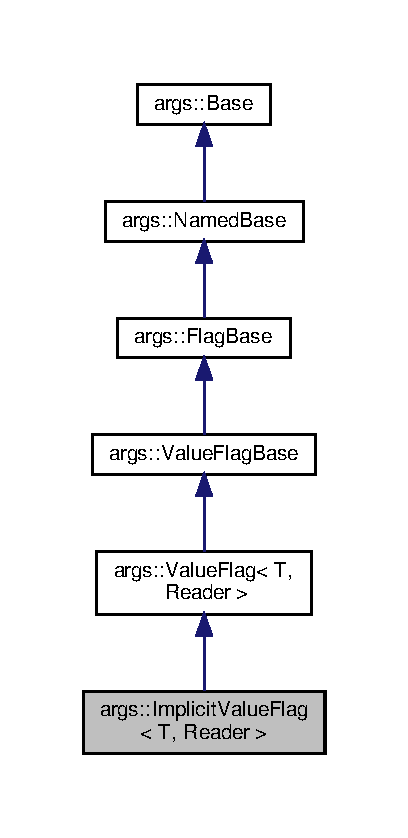
\includegraphics[width=196pt]{classargs_1_1_implicit_value_flag__inherit__graph}
\end{center}
\end{figure}


Collaboration diagram for args\+:\+:Implicit\+Value\+Flag$<$ T, Reader $>$\+:\nopagebreak
\begin{figure}[H]
\begin{center}
\leavevmode
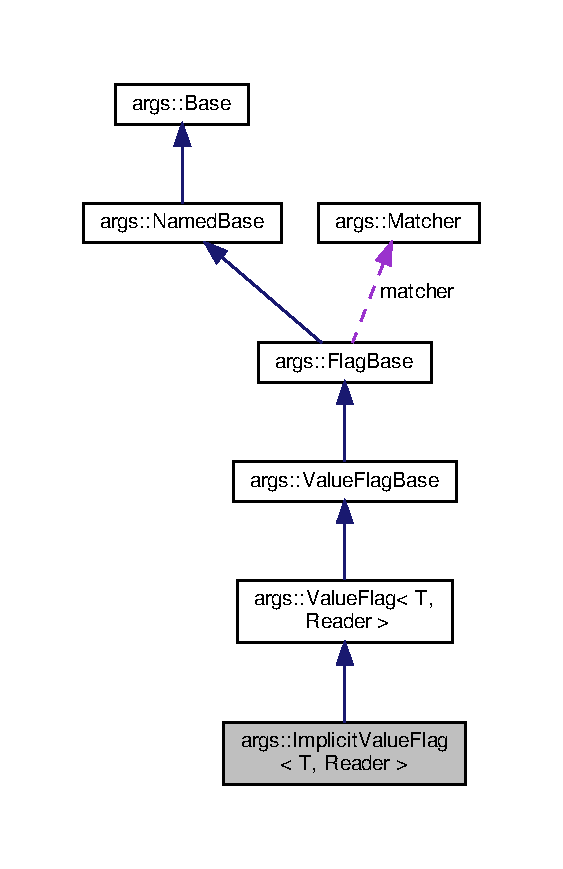
\includegraphics[width=270pt]{classargs_1_1_implicit_value_flag__coll__graph}
\end{center}
\end{figure}
\subsection*{Public Member Functions}
\begin{DoxyCompactItemize}
\item 
\hyperlink{classargs_1_1_implicit_value_flag_a666c1c0eca8615180da70ca76d446594}{Implicit\+Value\+Flag} (\hyperlink{classargs_1_1_group}{Group} \&group\+\_\+, const std\+::string \&name\+\_\+, const std\+::string \&help\+\_\+, \hyperlink{classargs_1_1_matcher}{Matcher} \&\&matcher\+\_\+, const T \&implicit\+Value\+\_\+, const T \&default\+Value\+\_\+=T(), \hyperlink{namespaceargs_aa530c0f95194aa275f49a5f299ac9e77}{Options} options\+\_\+=\{\})
\item 
\hyperlink{classargs_1_1_implicit_value_flag_aa2dd8fbab60032df5027d80962a5743d}{Implicit\+Value\+Flag} (\hyperlink{classargs_1_1_group}{Group} \&group\+\_\+, const std\+::string \&name\+\_\+, const std\+::string \&help\+\_\+, \hyperlink{classargs_1_1_matcher}{Matcher} \&\&matcher\+\_\+, const T \&default\+Value\+\_\+=T(), \hyperlink{namespaceargs_aa530c0f95194aa275f49a5f299ac9e77}{Options} options\+\_\+=\{\})
\item 
\hyperlink{classargs_1_1_implicit_value_flag_aa83bd9cd565c0e265e293c856ae0d119}{Implicit\+Value\+Flag} (\hyperlink{classargs_1_1_group}{Group} \&group\+\_\+, const std\+::string \&name\+\_\+, const std\+::string \&help\+\_\+, \hyperlink{classargs_1_1_matcher}{Matcher} \&\&matcher\+\_\+, \hyperlink{namespaceargs_aa530c0f95194aa275f49a5f299ac9e77}{Options} options\+\_\+)
\item 
virtual \hyperlink{classargs_1_1_implicit_value_flag_ac075d9514ac7d6907d2f26fd2fa078e2}{$\sim$\+Implicit\+Value\+Flag} ()
\item 
virtual \hyperlink{structargs_1_1_nargs}{Nargs} \hyperlink{classargs_1_1_implicit_value_flag_a7cfc67aca2b32921e722f51d349df2c5}{Number\+Of\+Arguments} () const noexcept override
\item 
virtual void \hyperlink{classargs_1_1_implicit_value_flag_a4c3124a516ca870903c4788dce781292}{Parse\+Value} (const std\+::vector$<$ std\+::string $>$ \&value\+\_\+) override
\end{DoxyCompactItemize}
\subsection*{Protected Attributes}
\begin{DoxyCompactItemize}
\item 
T \hyperlink{classargs_1_1_implicit_value_flag_a3cd2d0dac7fc96c4518608bb1525d934}{implicit\+Value}
\end{DoxyCompactItemize}
\subsection*{Additional Inherited Members}


\subsection{Detailed Description}
\subsubsection*{template$<$typename T, typename Reader = Value\+Reader$>$\newline
class args\+::\+Implicit\+Value\+Flag$<$ T, Reader $>$}

An optional argument-\/accepting flag class


\begin{DoxyTemplParams}{Template Parameters}
{\em T} & the type to extract the argument as \\
\hline
{\em Reader} & The functor type used to read the argument, taking the name, value, and destination reference with operator(), and returning a bool (if A\+R\+G\+S\+\_\+\+N\+O\+E\+X\+C\+E\+PT is defined) \\
\hline
\end{DoxyTemplParams}


\subsection{Constructor \& Destructor Documentation}
\mbox{\Hypertarget{classargs_1_1_implicit_value_flag_a666c1c0eca8615180da70ca76d446594}\label{classargs_1_1_implicit_value_flag_a666c1c0eca8615180da70ca76d446594}} 
\index{args\+::\+Implicit\+Value\+Flag@{args\+::\+Implicit\+Value\+Flag}!Implicit\+Value\+Flag@{Implicit\+Value\+Flag}}
\index{Implicit\+Value\+Flag@{Implicit\+Value\+Flag}!args\+::\+Implicit\+Value\+Flag@{args\+::\+Implicit\+Value\+Flag}}
\subsubsection{\texorpdfstring{Implicit\+Value\+Flag()}{ImplicitValueFlag()}\hspace{0.1cm}{\footnotesize\ttfamily [1/3]}}
{\footnotesize\ttfamily template$<$typename T , typename Reader  = Value\+Reader$>$ \\
\hyperlink{classargs_1_1_implicit_value_flag}{args\+::\+Implicit\+Value\+Flag}$<$ T, Reader $>$\+::\hyperlink{classargs_1_1_implicit_value_flag}{Implicit\+Value\+Flag} (\begin{DoxyParamCaption}\item[{\hyperlink{classargs_1_1_group}{Group} \&}]{group\+\_\+,  }\item[{const std\+::string \&}]{name\+\_\+,  }\item[{const std\+::string \&}]{help\+\_\+,  }\item[{\hyperlink{classargs_1_1_matcher}{Matcher} \&\&}]{matcher\+\_\+,  }\item[{const T \&}]{implicit\+Value\+\_\+,  }\item[{const T \&}]{default\+Value\+\_\+ = {\ttfamily T()},  }\item[{\hyperlink{namespaceargs_aa530c0f95194aa275f49a5f299ac9e77}{Options}}]{options\+\_\+ = {\ttfamily \{\}} }\end{DoxyParamCaption})\hspace{0.3cm}{\ttfamily [inline]}}

\mbox{\Hypertarget{classargs_1_1_implicit_value_flag_aa2dd8fbab60032df5027d80962a5743d}\label{classargs_1_1_implicit_value_flag_aa2dd8fbab60032df5027d80962a5743d}} 
\index{args\+::\+Implicit\+Value\+Flag@{args\+::\+Implicit\+Value\+Flag}!Implicit\+Value\+Flag@{Implicit\+Value\+Flag}}
\index{Implicit\+Value\+Flag@{Implicit\+Value\+Flag}!args\+::\+Implicit\+Value\+Flag@{args\+::\+Implicit\+Value\+Flag}}
\subsubsection{\texorpdfstring{Implicit\+Value\+Flag()}{ImplicitValueFlag()}\hspace{0.1cm}{\footnotesize\ttfamily [2/3]}}
{\footnotesize\ttfamily template$<$typename T , typename Reader  = Value\+Reader$>$ \\
\hyperlink{classargs_1_1_implicit_value_flag}{args\+::\+Implicit\+Value\+Flag}$<$ T, Reader $>$\+::\hyperlink{classargs_1_1_implicit_value_flag}{Implicit\+Value\+Flag} (\begin{DoxyParamCaption}\item[{\hyperlink{classargs_1_1_group}{Group} \&}]{group\+\_\+,  }\item[{const std\+::string \&}]{name\+\_\+,  }\item[{const std\+::string \&}]{help\+\_\+,  }\item[{\hyperlink{classargs_1_1_matcher}{Matcher} \&\&}]{matcher\+\_\+,  }\item[{const T \&}]{default\+Value\+\_\+ = {\ttfamily T()},  }\item[{\hyperlink{namespaceargs_aa530c0f95194aa275f49a5f299ac9e77}{Options}}]{options\+\_\+ = {\ttfamily \{\}} }\end{DoxyParamCaption})\hspace{0.3cm}{\ttfamily [inline]}}

\mbox{\Hypertarget{classargs_1_1_implicit_value_flag_aa83bd9cd565c0e265e293c856ae0d119}\label{classargs_1_1_implicit_value_flag_aa83bd9cd565c0e265e293c856ae0d119}} 
\index{args\+::\+Implicit\+Value\+Flag@{args\+::\+Implicit\+Value\+Flag}!Implicit\+Value\+Flag@{Implicit\+Value\+Flag}}
\index{Implicit\+Value\+Flag@{Implicit\+Value\+Flag}!args\+::\+Implicit\+Value\+Flag@{args\+::\+Implicit\+Value\+Flag}}
\subsubsection{\texorpdfstring{Implicit\+Value\+Flag()}{ImplicitValueFlag()}\hspace{0.1cm}{\footnotesize\ttfamily [3/3]}}
{\footnotesize\ttfamily template$<$typename T , typename Reader  = Value\+Reader$>$ \\
\hyperlink{classargs_1_1_implicit_value_flag}{args\+::\+Implicit\+Value\+Flag}$<$ T, Reader $>$\+::\hyperlink{classargs_1_1_implicit_value_flag}{Implicit\+Value\+Flag} (\begin{DoxyParamCaption}\item[{\hyperlink{classargs_1_1_group}{Group} \&}]{group\+\_\+,  }\item[{const std\+::string \&}]{name\+\_\+,  }\item[{const std\+::string \&}]{help\+\_\+,  }\item[{\hyperlink{classargs_1_1_matcher}{Matcher} \&\&}]{matcher\+\_\+,  }\item[{\hyperlink{namespaceargs_aa530c0f95194aa275f49a5f299ac9e77}{Options}}]{options\+\_\+ }\end{DoxyParamCaption})\hspace{0.3cm}{\ttfamily [inline]}}

\mbox{\Hypertarget{classargs_1_1_implicit_value_flag_ac075d9514ac7d6907d2f26fd2fa078e2}\label{classargs_1_1_implicit_value_flag_ac075d9514ac7d6907d2f26fd2fa078e2}} 
\index{args\+::\+Implicit\+Value\+Flag@{args\+::\+Implicit\+Value\+Flag}!````~Implicit\+Value\+Flag@{$\sim$\+Implicit\+Value\+Flag}}
\index{````~Implicit\+Value\+Flag@{$\sim$\+Implicit\+Value\+Flag}!args\+::\+Implicit\+Value\+Flag@{args\+::\+Implicit\+Value\+Flag}}
\subsubsection{\texorpdfstring{$\sim$\+Implicit\+Value\+Flag()}{~ImplicitValueFlag()}}
{\footnotesize\ttfamily template$<$typename T , typename Reader  = Value\+Reader$>$ \\
virtual \hyperlink{classargs_1_1_implicit_value_flag}{args\+::\+Implicit\+Value\+Flag}$<$ T, Reader $>$\+::$\sim$\hyperlink{classargs_1_1_implicit_value_flag}{Implicit\+Value\+Flag} (\begin{DoxyParamCaption}{ }\end{DoxyParamCaption})\hspace{0.3cm}{\ttfamily [inline]}, {\ttfamily [virtual]}}



\subsection{Member Function Documentation}
\mbox{\Hypertarget{classargs_1_1_implicit_value_flag_a7cfc67aca2b32921e722f51d349df2c5}\label{classargs_1_1_implicit_value_flag_a7cfc67aca2b32921e722f51d349df2c5}} 
\index{args\+::\+Implicit\+Value\+Flag@{args\+::\+Implicit\+Value\+Flag}!Number\+Of\+Arguments@{Number\+Of\+Arguments}}
\index{Number\+Of\+Arguments@{Number\+Of\+Arguments}!args\+::\+Implicit\+Value\+Flag@{args\+::\+Implicit\+Value\+Flag}}
\subsubsection{\texorpdfstring{Number\+Of\+Arguments()}{NumberOfArguments()}}
{\footnotesize\ttfamily template$<$typename T , typename Reader  = Value\+Reader$>$ \\
virtual \hyperlink{structargs_1_1_nargs}{Nargs} \hyperlink{classargs_1_1_implicit_value_flag}{args\+::\+Implicit\+Value\+Flag}$<$ T, Reader $>$\+::Number\+Of\+Arguments (\begin{DoxyParamCaption}{ }\end{DoxyParamCaption}) const\hspace{0.3cm}{\ttfamily [inline]}, {\ttfamily [override]}, {\ttfamily [virtual]}, {\ttfamily [noexcept]}}

Defines how many values can be consumed by this option.

\begin{DoxyReturn}{Returns}
closed interval \mbox{[}min, max\mbox{]} 
\end{DoxyReturn}


Reimplemented from \hyperlink{classargs_1_1_value_flag_base_a96a10bfb949ad175dcf2ffba6a6ec3b6}{args\+::\+Value\+Flag\+Base}.

\mbox{\Hypertarget{classargs_1_1_implicit_value_flag_a4c3124a516ca870903c4788dce781292}\label{classargs_1_1_implicit_value_flag_a4c3124a516ca870903c4788dce781292}} 
\index{args\+::\+Implicit\+Value\+Flag@{args\+::\+Implicit\+Value\+Flag}!Parse\+Value@{Parse\+Value}}
\index{Parse\+Value@{Parse\+Value}!args\+::\+Implicit\+Value\+Flag@{args\+::\+Implicit\+Value\+Flag}}
\subsubsection{\texorpdfstring{Parse\+Value()}{ParseValue()}}
{\footnotesize\ttfamily template$<$typename T , typename Reader  = Value\+Reader$>$ \\
virtual void \hyperlink{classargs_1_1_implicit_value_flag}{args\+::\+Implicit\+Value\+Flag}$<$ T, Reader $>$\+::Parse\+Value (\begin{DoxyParamCaption}\item[{const std\+::vector$<$ std\+::string $>$ \&}]{value }\end{DoxyParamCaption})\hspace{0.3cm}{\ttfamily [inline]}, {\ttfamily [override]}, {\ttfamily [virtual]}}

Parse values of this option.


\begin{DoxyParams}{Parameters}
{\em value} & Vector of values. It\textquotesingle{}s size must be in \hyperlink{classargs_1_1_implicit_value_flag_a7cfc67aca2b32921e722f51d349df2c5}{Number\+Of\+Arguments()} interval. \\
\hline
\end{DoxyParams}


Reimplemented from \hyperlink{classargs_1_1_value_flag_af3a872ae8fb0fa34814cbc7e133aa9bf}{args\+::\+Value\+Flag$<$ T, Reader $>$}.



\subsection{Member Data Documentation}
\mbox{\Hypertarget{classargs_1_1_implicit_value_flag_a3cd2d0dac7fc96c4518608bb1525d934}\label{classargs_1_1_implicit_value_flag_a3cd2d0dac7fc96c4518608bb1525d934}} 
\index{args\+::\+Implicit\+Value\+Flag@{args\+::\+Implicit\+Value\+Flag}!implicit\+Value@{implicit\+Value}}
\index{implicit\+Value@{implicit\+Value}!args\+::\+Implicit\+Value\+Flag@{args\+::\+Implicit\+Value\+Flag}}
\subsubsection{\texorpdfstring{implicit\+Value}{implicitValue}}
{\footnotesize\ttfamily template$<$typename T , typename Reader  = Value\+Reader$>$ \\
T \hyperlink{classargs_1_1_implicit_value_flag}{args\+::\+Implicit\+Value\+Flag}$<$ T, Reader $>$\+::implicit\+Value\hspace{0.3cm}{\ttfamily [protected]}}



The documentation for this class was generated from the following file\+:\begin{DoxyCompactItemize}
\item 
/home/cappelletto/github/self/landing\+\_\+area\+\_\+detector/external/\hyperlink{args_8hxx}{args.\+hxx}\end{DoxyCompactItemize}

\hypertarget{structargs_1_1detail_1_1_is_convertable_to_string}{}\section{args\+:\+:detail\+:\+:Is\+Convertable\+To\+String$<$ T, typename $>$ Struct Template Reference}
\label{structargs_1_1detail_1_1_is_convertable_to_string}\index{args\+::detail\+::\+Is\+Convertable\+To\+String$<$ T, typename $>$@{args\+::detail\+::\+Is\+Convertable\+To\+String$<$ T, typename $>$}}


{\ttfamily \#include $<$args.\+hxx$>$}



Inheritance diagram for args\+:\+:detail\+:\+:Is\+Convertable\+To\+String$<$ T, typename $>$\+:\nopagebreak
\begin{figure}[H]
\begin{center}
\leavevmode
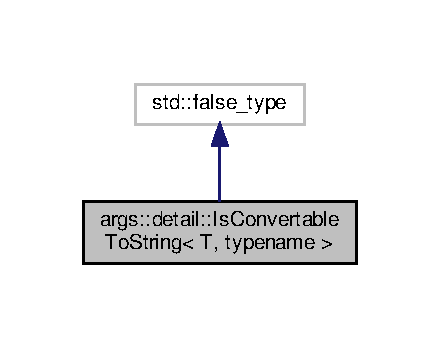
\includegraphics[width=211pt]{structargs_1_1detail_1_1_is_convertable_to_string__inherit__graph}
\end{center}
\end{figure}


Collaboration diagram for args\+:\+:detail\+:\+:Is\+Convertable\+To\+String$<$ T, typename $>$\+:\nopagebreak
\begin{figure}[H]
\begin{center}
\leavevmode
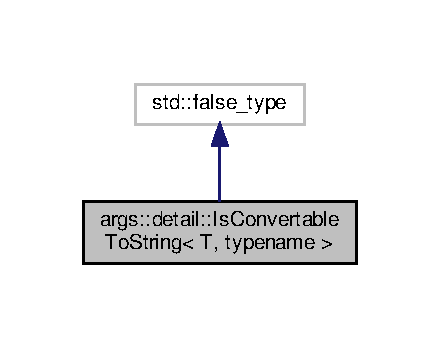
\includegraphics[width=211pt]{structargs_1_1detail_1_1_is_convertable_to_string__coll__graph}
\end{center}
\end{figure}


The documentation for this struct was generated from the following file\+:\begin{DoxyCompactItemize}
\item 
/home/cappelletto/github/self/landing\+\_\+area\+\_\+detector/external/\hyperlink{args_8hxx}{args.\+hxx}\end{DoxyCompactItemize}

\hypertarget{classlad_1_1_kernel_layer}{}\section{lad\+:\+:Kernel\+Layer Class Reference}
\label{classlad_1_1_kernel_layer}\index{lad\+::\+Kernel\+Layer@{lad\+::\+Kernel\+Layer}}


{\ttfamily \#include $<$lad\+\_\+layer.\+hpp$>$}



Inheritance diagram for lad\+:\+:Kernel\+Layer\+:\nopagebreak
\begin{figure}[H]
\begin{center}
\leavevmode
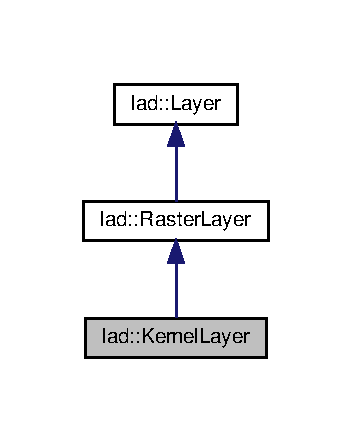
\includegraphics[width=169pt]{classlad_1_1_kernel_layer__inherit__graph}
\end{center}
\end{figure}


Collaboration diagram for lad\+:\+:Kernel\+Layer\+:\nopagebreak
\begin{figure}[H]
\begin{center}
\leavevmode
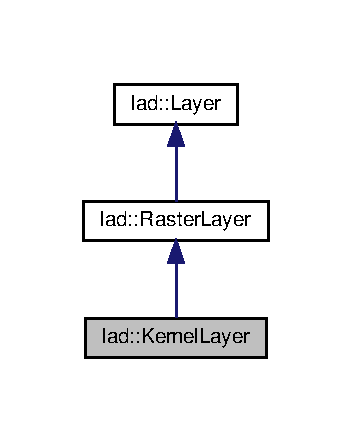
\includegraphics[width=169pt]{classlad_1_1_kernel_layer__coll__graph}
\end{center}
\end{figure}
\subsection*{Public Attributes}
\begin{DoxyCompactItemize}
\item 
double \hyperlink{classlad_1_1_kernel_layer_a41e48b8aa5359019629a156dd9868c17}{d\+Rotation}
\begin{DoxyCompactList}\small\item\em Rotation angle of the given kernel (in radians) \end{DoxyCompactList}\end{DoxyCompactItemize}
\subsection*{Additional Inherited Members}


\subsection{Member Data Documentation}
\mbox{\Hypertarget{classlad_1_1_kernel_layer_a41e48b8aa5359019629a156dd9868c17}\label{classlad_1_1_kernel_layer_a41e48b8aa5359019629a156dd9868c17}} 
\index{lad\+::\+Kernel\+Layer@{lad\+::\+Kernel\+Layer}!d\+Rotation@{d\+Rotation}}
\index{d\+Rotation@{d\+Rotation}!lad\+::\+Kernel\+Layer@{lad\+::\+Kernel\+Layer}}
\subsubsection{\texorpdfstring{d\+Rotation}{dRotation}}
{\footnotesize\ttfamily double lad\+::\+Kernel\+Layer\+::d\+Rotation}



Rotation angle of the given kernel (in radians) 



The documentation for this class was generated from the following file\+:\begin{DoxyCompactItemize}
\item 
/home/cappelletto/github/self/landing\+\_\+area\+\_\+detector/include/\hyperlink{lad__layer_8hpp}{lad\+\_\+layer.\+hpp}\end{DoxyCompactItemize}

\hypertarget{classlad_1_1lad_pipeline}{}\section{lad\+:\+:lad\+Pipeline Class Reference}
\label{classlad_1_1lad_pipeline}\index{lad\+::lad\+Pipeline@{lad\+::lad\+Pipeline}}


$<$ landing area detection algorithm namespace  




{\ttfamily \#include $<$lad\+\_\+core.\+hpp$>$}



Collaboration diagram for lad\+:\+:lad\+Pipeline\+:\nopagebreak
\begin{figure}[H]
\begin{center}
\leavevmode
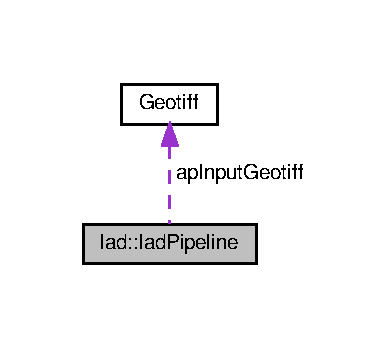
\includegraphics[width=187pt]{classlad_1_1lad_pipeline__coll__graph}
\end{center}
\end{figure}
\subsection*{Public Member Functions}
\begin{DoxyCompactItemize}
\item 
\hyperlink{classlad_1_1lad_pipeline_a47ebdd8f4797a0a7ea562682e2f311c3}{lad\+Pipeline} ()
\item 
int \hyperlink{classlad_1_1lad_pipeline_a60959c4c046e112741f87fa37fa08d9b}{Read\+T\+I\+FF} (std\+::string input\+File)
\begin{DoxyCompactList}\small\item\em Read a given geo\+T\+I\+FF file an loads into current container. \end{DoxyCompactList}\item 
std\+::string \hyperlink{classlad_1_1lad_pipeline_a10c0af216e3004e054d351b9f517408b}{Get\+Layer\+Name} (int id)
\begin{DoxyCompactList}\small\item\em Returns name of \hyperlink{classlad_1_1_layer}{Layer} with given ID number. \end{DoxyCompactList}\item 
int \hyperlink{classlad_1_1lad_pipeline_a6e4748a05ef0346e1912118496931523}{Get\+Vector\+ID} (std\+::string name)
\begin{DoxyCompactList}\small\item\em Return first vector that matches \textquotesingle{}name\textquotesingle{} as layer name. \end{DoxyCompactList}\item 
int \hyperlink{classlad_1_1lad_pipeline_a05a4d4197caa86b14bbbfe53237bfab0}{Set\+Layer\+Name} (int id, std\+::string new\+Name)
\begin{DoxyCompactList}\small\item\em Overwrite Layers name using is ID. \end{DoxyCompactList}\end{DoxyCompactItemize}
\subsection*{Public Attributes}
\begin{DoxyCompactItemize}
\item 
\hyperlink{class_geotiff}{Geotiff} $\ast$ \hyperlink{classlad_1_1lad_pipeline_a1ecbd2ad5ac586de2876ee2e59cc1b97}{ap\+Input\+Geotiff}
\begin{DoxyCompactList}\small\item\em landing area detection algorithm namespace \end{DoxyCompactList}\item 
std\+::string \hyperlink{classlad_1_1lad_pipeline_a2312bba58d0b3b44e72fd6bea4e4b35c}{input\+File\+T\+I\+FF}
\begin{DoxyCompactList}\small\item\em Input T\+I\+FF filename containing base bathymetry. Base name for output products files. \end{DoxyCompactList}\item 
vector$<$ std\+::shared\+\_\+ptr$<$ \hyperlink{classlad_1_1_layer}{Layer} $>$ $>$ \hyperlink{classlad_1_1lad_pipeline_a7c0702fe312deebd185bd3a3a5a02a53}{Layers}
\begin{DoxyCompactList}\small\item\em Collection of layers. Using smart shared pointers for tree-\/like pipeline structures. \end{DoxyCompactList}\end{DoxyCompactItemize}


\subsection{Detailed Description}
$<$ landing area detection algorithm namespace 

\subsection{Constructor \& Destructor Documentation}
\mbox{\Hypertarget{classlad_1_1lad_pipeline_a47ebdd8f4797a0a7ea562682e2f311c3}\label{classlad_1_1lad_pipeline_a47ebdd8f4797a0a7ea562682e2f311c3}} 
\index{lad\+::lad\+Pipeline@{lad\+::lad\+Pipeline}!lad\+Pipeline@{lad\+Pipeline}}
\index{lad\+Pipeline@{lad\+Pipeline}!lad\+::lad\+Pipeline@{lad\+::lad\+Pipeline}}
\subsubsection{\texorpdfstring{lad\+Pipeline()}{ladPipeline()}}
{\footnotesize\ttfamily lad\+::lad\+Pipeline\+::lad\+Pipeline (\begin{DoxyParamCaption}{ }\end{DoxyParamCaption})\hspace{0.3cm}{\ttfamily [inline]}}



\subsection{Member Function Documentation}
\mbox{\Hypertarget{classlad_1_1lad_pipeline_a10c0af216e3004e054d351b9f517408b}\label{classlad_1_1lad_pipeline_a10c0af216e3004e054d351b9f517408b}} 
\index{lad\+::lad\+Pipeline@{lad\+::lad\+Pipeline}!Get\+Layer\+Name@{Get\+Layer\+Name}}
\index{Get\+Layer\+Name@{Get\+Layer\+Name}!lad\+::lad\+Pipeline@{lad\+::lad\+Pipeline}}
\subsubsection{\texorpdfstring{Get\+Layer\+Name()}{GetLayerName()}}
{\footnotesize\ttfamily std\+::string lad\+::lad\+Pipeline\+::\+Get\+Layer\+Name (\begin{DoxyParamCaption}\item[{int}]{id }\end{DoxyParamCaption})}



Returns name of \hyperlink{classlad_1_1_layer}{Layer} with given ID number. 

Returns (if present) the name of the vector layer that matches provided ID.


\begin{DoxyParams}{Parameters}
{\em id} & \hyperlink{classlad_1_1_layer}{Layer} ID number to be searched \\
\hline
\end{DoxyParams}
\begin{DoxyReturn}{Returns}
std\+::string 
\end{DoxyReturn}
\mbox{\Hypertarget{classlad_1_1lad_pipeline_a6e4748a05ef0346e1912118496931523}\label{classlad_1_1lad_pipeline_a6e4748a05ef0346e1912118496931523}} 
\index{lad\+::lad\+Pipeline@{lad\+::lad\+Pipeline}!Get\+Vector\+ID@{Get\+Vector\+ID}}
\index{Get\+Vector\+ID@{Get\+Vector\+ID}!lad\+::lad\+Pipeline@{lad\+::lad\+Pipeline}}
\subsubsection{\texorpdfstring{Get\+Vector\+I\+D()}{GetVectorID()}}
{\footnotesize\ttfamily int lad\+::lad\+Pipeline\+::\+Get\+Vector\+ID (\begin{DoxyParamCaption}\item[{std\+::string}]{name }\end{DoxyParamCaption})}



Return first vector that matches \textquotesingle{}name\textquotesingle{} as layer name. 

\mbox{\Hypertarget{classlad_1_1lad_pipeline_a60959c4c046e112741f87fa37fa08d9b}\label{classlad_1_1lad_pipeline_a60959c4c046e112741f87fa37fa08d9b}} 
\index{lad\+::lad\+Pipeline@{lad\+::lad\+Pipeline}!Read\+T\+I\+FF@{Read\+T\+I\+FF}}
\index{Read\+T\+I\+FF@{Read\+T\+I\+FF}!lad\+::lad\+Pipeline@{lad\+::lad\+Pipeline}}
\subsubsection{\texorpdfstring{Read\+T\+I\+F\+F()}{ReadTIFF()}}
{\footnotesize\ttfamily int lad\+::lad\+Pipeline\+::\+Read\+T\+I\+FF (\begin{DoxyParamCaption}\item[{std\+::string}]{input\+File }\end{DoxyParamCaption})}



Read a given geo\+T\+I\+FF file an loads into current container. 

\mbox{\Hypertarget{classlad_1_1lad_pipeline_a05a4d4197caa86b14bbbfe53237bfab0}\label{classlad_1_1lad_pipeline_a05a4d4197caa86b14bbbfe53237bfab0}} 
\index{lad\+::lad\+Pipeline@{lad\+::lad\+Pipeline}!Set\+Layer\+Name@{Set\+Layer\+Name}}
\index{Set\+Layer\+Name@{Set\+Layer\+Name}!lad\+::lad\+Pipeline@{lad\+::lad\+Pipeline}}
\subsubsection{\texorpdfstring{Set\+Layer\+Name()}{SetLayerName()}}
{\footnotesize\ttfamily int lad\+::lad\+Pipeline\+::\+Set\+Layer\+Name (\begin{DoxyParamCaption}\item[{int}]{id,  }\item[{std\+::string}]{new\+Name }\end{DoxyParamCaption})}



Overwrite Layers name using is ID. 

Overwrite the name of a layer (if present) with a unique string.

If provided string 
\begin{DoxyParams}{Parameters}
{\em id} & \\
\hline
\end{DoxyParams}
\begin{DoxyReturn}{Returns}
std\+::string 
\end{DoxyReturn}


\subsection{Member Data Documentation}
\mbox{\Hypertarget{classlad_1_1lad_pipeline_a1ecbd2ad5ac586de2876ee2e59cc1b97}\label{classlad_1_1lad_pipeline_a1ecbd2ad5ac586de2876ee2e59cc1b97}} 
\index{lad\+::lad\+Pipeline@{lad\+::lad\+Pipeline}!ap\+Input\+Geotiff@{ap\+Input\+Geotiff}}
\index{ap\+Input\+Geotiff@{ap\+Input\+Geotiff}!lad\+::lad\+Pipeline@{lad\+::lad\+Pipeline}}
\subsubsection{\texorpdfstring{ap\+Input\+Geotiff}{apInputGeotiff}}
{\footnotesize\ttfamily \hyperlink{class_geotiff}{Geotiff}$\ast$ lad\+::lad\+Pipeline\+::ap\+Input\+Geotiff}



landing area detection algorithm namespace 

\mbox{\Hypertarget{classlad_1_1lad_pipeline_a2312bba58d0b3b44e72fd6bea4e4b35c}\label{classlad_1_1lad_pipeline_a2312bba58d0b3b44e72fd6bea4e4b35c}} 
\index{lad\+::lad\+Pipeline@{lad\+::lad\+Pipeline}!input\+File\+T\+I\+FF@{input\+File\+T\+I\+FF}}
\index{input\+File\+T\+I\+FF@{input\+File\+T\+I\+FF}!lad\+::lad\+Pipeline@{lad\+::lad\+Pipeline}}
\subsubsection{\texorpdfstring{input\+File\+T\+I\+FF}{inputFileTIFF}}
{\footnotesize\ttfamily std\+::string lad\+::lad\+Pipeline\+::input\+File\+T\+I\+FF}



Input T\+I\+FF filename containing base bathymetry. Base name for output products files. 

\mbox{\Hypertarget{classlad_1_1lad_pipeline_a7c0702fe312deebd185bd3a3a5a02a53}\label{classlad_1_1lad_pipeline_a7c0702fe312deebd185bd3a3a5a02a53}} 
\index{lad\+::lad\+Pipeline@{lad\+::lad\+Pipeline}!Layers@{Layers}}
\index{Layers@{Layers}!lad\+::lad\+Pipeline@{lad\+::lad\+Pipeline}}
\subsubsection{\texorpdfstring{Layers}{Layers}}
{\footnotesize\ttfamily vector$<$std\+::shared\+\_\+ptr $<$\hyperlink{classlad_1_1_layer}{Layer}$>$ $>$ lad\+::lad\+Pipeline\+::\+Layers}



Collection of layers. Using smart shared pointers for tree-\/like pipeline structures. 



The documentation for this class was generated from the following files\+:\begin{DoxyCompactItemize}
\item 
/home/cappelletto/github/self/landing\+\_\+area\+\_\+detector/include/\hyperlink{lad__core_8hpp}{lad\+\_\+core.\+hpp}\item 
/home/cappelletto/github/self/landing\+\_\+area\+\_\+detector/src/\hyperlink{lad__core_8cpp}{lad\+\_\+core.\+cpp}\end{DoxyCompactItemize}

\hypertarget{classlad_1_1_layer}{}\section{lad\+:\+:Layer Class Reference}
\label{classlad_1_1_layer}\index{lad\+::\+Layer@{lad\+::\+Layer}}


$<$ landing area detection algorithm namespace  




{\ttfamily \#include $<$lad\+\_\+layer.\+hpp$>$}



Inheritance diagram for lad\+:\+:Layer\+:\nopagebreak
\begin{figure}[H]
\begin{center}
\leavevmode
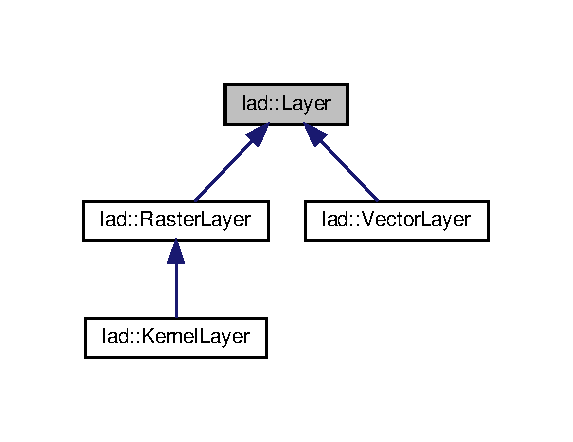
\includegraphics[width=275pt]{classlad_1_1_layer__inherit__graph}
\end{center}
\end{figure}
\subsection*{Public Member Functions}
\begin{DoxyCompactItemize}
\item 
\hyperlink{classlad_1_1_layer_a1a7d572812da1f17c292a0cfb977d4fe}{Layer} (std\+::string new\+Name=\char`\"{}noname\char`\"{})
\begin{DoxyCompactList}\small\item\em Construct a new \hyperlink{classlad_1_1_layer}{Layer} object. \end{DoxyCompactList}\item 
virtual \hyperlink{classlad_1_1_layer_abb04ca2570deb63ee685c3e8f74d872e}{$\sim$\+Layer} ()
\begin{DoxyCompactList}\small\item\em Virtual destructor of the \hyperlink{classlad_1_1_layer}{Layer} object. \end{DoxyCompactList}\item 
int \hyperlink{classlad_1_1_layer_a10a5e4b4cf9618129d57c960805b7607}{Get\+ID} ()
\begin{DoxyCompactList}\small\item\em Return the layer ID. \end{DoxyCompactList}\item 
int \hyperlink{classlad_1_1_layer_ae2d1e4d8d656967f9367555f6d960b7d}{Set\+ID} (int new\+ID)
\begin{DoxyCompactList}\small\item\em Set the new layer ID. It must be a valid ID. \end{DoxyCompactList}\item 
int \hyperlink{classlad_1_1_layer_a8223ec6cf99de0275118e20faa011bc9}{Get\+Layer\+Status} ()
\begin{DoxyCompactList}\small\item\em Return a copy of the layer status. \end{DoxyCompactList}\item 
int \hyperlink{classlad_1_1_layer_a7572fd2665a35c074b2f341ce8f73030}{Set\+Layerstatus} (int new\+Status)
\begin{DoxyCompactList}\small\item\em Modify the layer status. \end{DoxyCompactList}\item 
int \hyperlink{classlad_1_1_layer_aedd28090728135c4ae8a445f0d016b2c}{Get\+Layer\+Type} ()
\begin{DoxyCompactList}\small\item\em Return a copy of the layer type. \end{DoxyCompactList}\item 
int \hyperlink{classlad_1_1_layer_a178643063c5fb55f4010579731d3025b}{Set\+Layer\+Type} (int new\+Type)
\begin{DoxyCompactList}\small\item\em Modify the layer type. \end{DoxyCompactList}\end{DoxyCompactItemize}
\subsection*{Public Attributes}
\begin{DoxyCompactItemize}
\item 
std\+::string \hyperlink{classlad_1_1_layer_aadee8f64504428828f92591090f4f27d}{layer\+Name}
\begin{DoxyCompactList}\small\item\em \hyperlink{classlad_1_1_layer}{Layer} name. \end{DoxyCompactList}\item 
std\+::string \hyperlink{classlad_1_1_layer_a45420738ed98b38b86b863d1330c54f3}{layer\+File\+Name}
\begin{DoxyCompactList}\small\item\em Name of associated output file. \end{DoxyCompactList}\end{DoxyCompactItemize}


\subsection{Detailed Description}
$<$ landing area detection algorithm namespace 

\subsection{Constructor \& Destructor Documentation}
\mbox{\Hypertarget{classlad_1_1_layer_a1a7d572812da1f17c292a0cfb977d4fe}\label{classlad_1_1_layer_a1a7d572812da1f17c292a0cfb977d4fe}} 
\index{lad\+::\+Layer@{lad\+::\+Layer}!Layer@{Layer}}
\index{Layer@{Layer}!lad\+::\+Layer@{lad\+::\+Layer}}
\subsubsection{\texorpdfstring{Layer()}{Layer()}}
{\footnotesize\ttfamily lad\+::\+Layer\+::\+Layer (\begin{DoxyParamCaption}\item[{std\+::string}]{new\+Name = {\ttfamily \char`\"{}noname\char`\"{}} }\end{DoxyParamCaption})\hspace{0.3cm}{\ttfamily [inline]}}



Construct a new \hyperlink{classlad_1_1_layer}{Layer} object. 


\begin{DoxyParams}{Parameters}
{\em new\+Name} & Optional layer name. \char`\"{}noname\char`\"{} if none is specified at construction time \\
\hline
\end{DoxyParams}
\mbox{\Hypertarget{classlad_1_1_layer_abb04ca2570deb63ee685c3e8f74d872e}\label{classlad_1_1_layer_abb04ca2570deb63ee685c3e8f74d872e}} 
\index{lad\+::\+Layer@{lad\+::\+Layer}!````~Layer@{$\sim$\+Layer}}
\index{````~Layer@{$\sim$\+Layer}!lad\+::\+Layer@{lad\+::\+Layer}}
\subsubsection{\texorpdfstring{$\sim$\+Layer()}{~Layer()}}
{\footnotesize\ttfamily virtual lad\+::\+Layer\+::$\sim$\+Layer (\begin{DoxyParamCaption}{ }\end{DoxyParamCaption})\hspace{0.3cm}{\ttfamily [inline]}, {\ttfamily [virtual]}}



Virtual destructor of the \hyperlink{classlad_1_1_layer}{Layer} object. 

Depending on the type of container in the inherited instances, a type specific cleanup may be required 

\subsection{Member Function Documentation}
\mbox{\Hypertarget{classlad_1_1_layer_a10a5e4b4cf9618129d57c960805b7607}\label{classlad_1_1_layer_a10a5e4b4cf9618129d57c960805b7607}} 
\index{lad\+::\+Layer@{lad\+::\+Layer}!Get\+ID@{Get\+ID}}
\index{Get\+ID@{Get\+ID}!lad\+::\+Layer@{lad\+::\+Layer}}
\subsubsection{\texorpdfstring{Get\+I\+D()}{GetID()}}
{\footnotesize\ttfamily int lad\+::\+Layer\+::\+Get\+ID (\begin{DoxyParamCaption}{ }\end{DoxyParamCaption})}



Return the layer ID. 

Return the ID of the given layer.

\begin{DoxyReturn}{Returns}
int ID value 
\end{DoxyReturn}
\mbox{\Hypertarget{classlad_1_1_layer_a8223ec6cf99de0275118e20faa011bc9}\label{classlad_1_1_layer_a8223ec6cf99de0275118e20faa011bc9}} 
\index{lad\+::\+Layer@{lad\+::\+Layer}!Get\+Layer\+Status@{Get\+Layer\+Status}}
\index{Get\+Layer\+Status@{Get\+Layer\+Status}!lad\+::\+Layer@{lad\+::\+Layer}}
\subsubsection{\texorpdfstring{Get\+Layer\+Status()}{GetLayerStatus()}}
{\footnotesize\ttfamily int lad\+::\+Layer\+::\+Get\+Layer\+Status (\begin{DoxyParamCaption}{ }\end{DoxyParamCaption})}



Return a copy of the layer status. 

Get the \hyperlink{classlad_1_1_layer}{Layer} Status object.

\begin{DoxyReturn}{Returns}
int \hyperlink{classlad_1_1_layer}{Layer} status value, from enumerated list 
\end{DoxyReturn}
\mbox{\Hypertarget{classlad_1_1_layer_aedd28090728135c4ae8a445f0d016b2c}\label{classlad_1_1_layer_aedd28090728135c4ae8a445f0d016b2c}} 
\index{lad\+::\+Layer@{lad\+::\+Layer}!Get\+Layer\+Type@{Get\+Layer\+Type}}
\index{Get\+Layer\+Type@{Get\+Layer\+Type}!lad\+::\+Layer@{lad\+::\+Layer}}
\subsubsection{\texorpdfstring{Get\+Layer\+Type()}{GetLayerType()}}
{\footnotesize\ttfamily int lad\+::\+Layer\+::\+Get\+Layer\+Type (\begin{DoxyParamCaption}{ }\end{DoxyParamCaption})}



Return a copy of the layer type. 

Get the \hyperlink{classlad_1_1_layer}{Layer} Type object.

\begin{DoxyReturn}{Returns}
int Return the layer type, from enumerated list (R\+A\+S\+T\+ER, K\+E\+R\+N\+EL, V\+E\+C\+T\+OR, U\+N\+D\+E\+F\+I\+N\+ED) 
\end{DoxyReturn}
\mbox{\Hypertarget{classlad_1_1_layer_ae2d1e4d8d656967f9367555f6d960b7d}\label{classlad_1_1_layer_ae2d1e4d8d656967f9367555f6d960b7d}} 
\index{lad\+::\+Layer@{lad\+::\+Layer}!Set\+ID@{Set\+ID}}
\index{Set\+ID@{Set\+ID}!lad\+::\+Layer@{lad\+::\+Layer}}
\subsubsection{\texorpdfstring{Set\+I\+D()}{SetID()}}
{\footnotesize\ttfamily int lad\+::\+Layer\+::\+Set\+ID (\begin{DoxyParamCaption}\item[{int}]{new\+ID }\end{DoxyParamCaption})}



Set the new layer ID. It must be a valid ID. 

Update the ID value of the layer.


\begin{DoxyParams}{Parameters}
{\em new\+ID} & New ID value of the value. It must be a valid ID \\
\hline
\end{DoxyParams}
\begin{DoxyReturn}{Returns}
int Error code, if any. If the provided ID is valid it will return L\+A\+Y\+E\+R\+\_\+\+OK 
\end{DoxyReturn}
\mbox{\Hypertarget{classlad_1_1_layer_a7572fd2665a35c074b2f341ce8f73030}\label{classlad_1_1_layer_a7572fd2665a35c074b2f341ce8f73030}} 
\index{lad\+::\+Layer@{lad\+::\+Layer}!Set\+Layerstatus@{Set\+Layerstatus}}
\index{Set\+Layerstatus@{Set\+Layerstatus}!lad\+::\+Layer@{lad\+::\+Layer}}
\subsubsection{\texorpdfstring{Set\+Layerstatus()}{SetLayerstatus()}}
{\footnotesize\ttfamily int lad\+::\+Layer\+::\+Set\+Layerstatus (\begin{DoxyParamCaption}\item[{int}]{new\+Status }\end{DoxyParamCaption})}



Modify the layer status. 

Update the \hyperlink{classlad_1_1_layer}{Layer} status.


\begin{DoxyParams}{Parameters}
{\em new\+Status} & New value of layer status. It should be any of possible values in the enumerated list. No validation is enforced \\
\hline
\end{DoxyParams}
\begin{DoxyReturn}{Returns}
int return a copy of the new status value 
\end{DoxyReturn}
\mbox{\Hypertarget{classlad_1_1_layer_a178643063c5fb55f4010579731d3025b}\label{classlad_1_1_layer_a178643063c5fb55f4010579731d3025b}} 
\index{lad\+::\+Layer@{lad\+::\+Layer}!Set\+Layer\+Type@{Set\+Layer\+Type}}
\index{Set\+Layer\+Type@{Set\+Layer\+Type}!lad\+::\+Layer@{lad\+::\+Layer}}
\subsubsection{\texorpdfstring{Set\+Layer\+Type()}{SetLayerType()}}
{\footnotesize\ttfamily int lad\+::\+Layer\+::\+Set\+Layer\+Type (\begin{DoxyParamCaption}\item[{int}]{new\+Type }\end{DoxyParamCaption})}



Modify the layer type. 

Update the \hyperlink{classlad_1_1_layer}{Layer} type.


\begin{DoxyParams}{Parameters}
{\em new\+Type} & New value of layer type. It is user\textquotesingle{}s responsability to correctly recast (if necessary) the data container accordingly \\
\hline
\end{DoxyParams}
\begin{DoxyReturn}{Returns}
int return a copy of the new layer type 
\end{DoxyReturn}


\subsection{Member Data Documentation}
\mbox{\Hypertarget{classlad_1_1_layer_a45420738ed98b38b86b863d1330c54f3}\label{classlad_1_1_layer_a45420738ed98b38b86b863d1330c54f3}} 
\index{lad\+::\+Layer@{lad\+::\+Layer}!layer\+File\+Name@{layer\+File\+Name}}
\index{layer\+File\+Name@{layer\+File\+Name}!lad\+::\+Layer@{lad\+::\+Layer}}
\subsubsection{\texorpdfstring{layer\+File\+Name}{layerFileName}}
{\footnotesize\ttfamily std\+::string lad\+::\+Layer\+::layer\+File\+Name}



Name of associated output file. 

\mbox{\Hypertarget{classlad_1_1_layer_aadee8f64504428828f92591090f4f27d}\label{classlad_1_1_layer_aadee8f64504428828f92591090f4f27d}} 
\index{lad\+::\+Layer@{lad\+::\+Layer}!layer\+Name@{layer\+Name}}
\index{layer\+Name@{layer\+Name}!lad\+::\+Layer@{lad\+::\+Layer}}
\subsubsection{\texorpdfstring{layer\+Name}{layerName}}
{\footnotesize\ttfamily std\+::string lad\+::\+Layer\+::layer\+Name}



\hyperlink{classlad_1_1_layer}{Layer} name. 



The documentation for this class was generated from the following files\+:\begin{DoxyCompactItemize}
\item 
/home/cappelletto/github/self/landing\+\_\+area\+\_\+detector/include/\hyperlink{lad__layer_8hpp}{lad\+\_\+layer.\+hpp}\item 
/home/cappelletto/github/self/landing\+\_\+area\+\_\+detector/src/\hyperlink{lad__layer_8cpp}{lad\+\_\+layer.\+cpp}\end{DoxyCompactItemize}

\hypertarget{classargs_1_1_map_error}{}\section{args\+:\+:Map\+Error Class Reference}
\label{classargs_1_1_map_error}\index{args\+::\+Map\+Error@{args\+::\+Map\+Error}}


{\ttfamily \#include $<$args.\+hxx$>$}



Inheritance diagram for args\+:\+:Map\+Error\+:\nopagebreak
\begin{figure}[H]
\begin{center}
\leavevmode
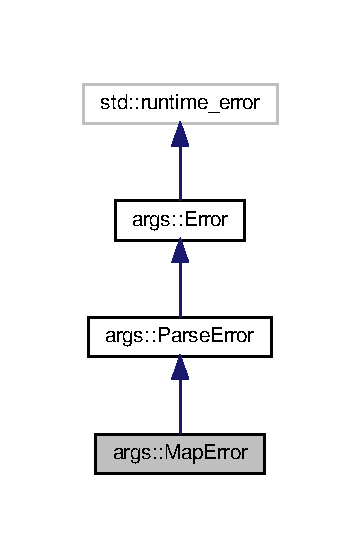
\includegraphics[width=173pt]{classargs_1_1_map_error__inherit__graph}
\end{center}
\end{figure}


Collaboration diagram for args\+:\+:Map\+Error\+:\nopagebreak
\begin{figure}[H]
\begin{center}
\leavevmode
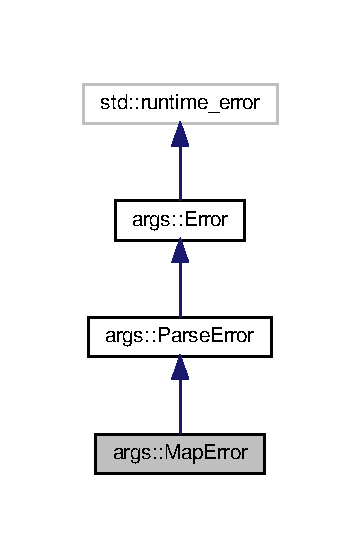
\includegraphics[width=173pt]{classargs_1_1_map_error__coll__graph}
\end{center}
\end{figure}
\subsection*{Public Member Functions}
\begin{DoxyCompactItemize}
\item 
\hyperlink{classargs_1_1_map_error_a5339dca0b3910dd978152b442adf9de4}{Map\+Error} (const std\+::string \&problem)
\item 
virtual \hyperlink{classargs_1_1_map_error_aa5d2acb7ec907a7aa85d52a346074125}{$\sim$\+Map\+Error} ()
\end{DoxyCompactItemize}


\subsection{Detailed Description}
Errors in map lookups 

\subsection{Constructor \& Destructor Documentation}
\mbox{\Hypertarget{classargs_1_1_map_error_a5339dca0b3910dd978152b442adf9de4}\label{classargs_1_1_map_error_a5339dca0b3910dd978152b442adf9de4}} 
\index{args\+::\+Map\+Error@{args\+::\+Map\+Error}!Map\+Error@{Map\+Error}}
\index{Map\+Error@{Map\+Error}!args\+::\+Map\+Error@{args\+::\+Map\+Error}}
\subsubsection{\texorpdfstring{Map\+Error()}{MapError()}}
{\footnotesize\ttfamily args\+::\+Map\+Error\+::\+Map\+Error (\begin{DoxyParamCaption}\item[{const std\+::string \&}]{problem }\end{DoxyParamCaption})\hspace{0.3cm}{\ttfamily [inline]}}

\mbox{\Hypertarget{classargs_1_1_map_error_aa5d2acb7ec907a7aa85d52a346074125}\label{classargs_1_1_map_error_aa5d2acb7ec907a7aa85d52a346074125}} 
\index{args\+::\+Map\+Error@{args\+::\+Map\+Error}!````~Map\+Error@{$\sim$\+Map\+Error}}
\index{````~Map\+Error@{$\sim$\+Map\+Error}!args\+::\+Map\+Error@{args\+::\+Map\+Error}}
\subsubsection{\texorpdfstring{$\sim$\+Map\+Error()}{~MapError()}}
{\footnotesize\ttfamily virtual args\+::\+Map\+Error\+::$\sim$\+Map\+Error (\begin{DoxyParamCaption}{ }\end{DoxyParamCaption})\hspace{0.3cm}{\ttfamily [inline]}, {\ttfamily [virtual]}}



The documentation for this class was generated from the following file\+:\begin{DoxyCompactItemize}
\item 
/home/cappelletto/github/self/landing\+\_\+area\+\_\+detector/external/\hyperlink{args_8hxx}{args.\+hxx}\end{DoxyCompactItemize}

\hypertarget{classargs_1_1_map_flag}{}\section{args\+:\+:Map\+Flag$<$ K, T, Reader, Map $>$ Class Template Reference}
\label{classargs_1_1_map_flag}\index{args\+::\+Map\+Flag$<$ K, T, Reader, Map $>$@{args\+::\+Map\+Flag$<$ K, T, Reader, Map $>$}}


{\ttfamily \#include $<$args.\+hxx$>$}



Inheritance diagram for args\+:\+:Map\+Flag$<$ K, T, Reader, Map $>$\+:\nopagebreak
\begin{figure}[H]
\begin{center}
\leavevmode
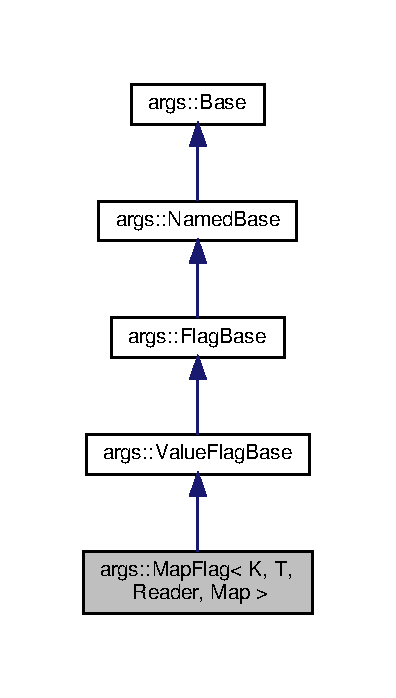
\includegraphics[width=190pt]{classargs_1_1_map_flag__inherit__graph}
\end{center}
\end{figure}


Collaboration diagram for args\+:\+:Map\+Flag$<$ K, T, Reader, Map $>$\+:\nopagebreak
\begin{figure}[H]
\begin{center}
\leavevmode
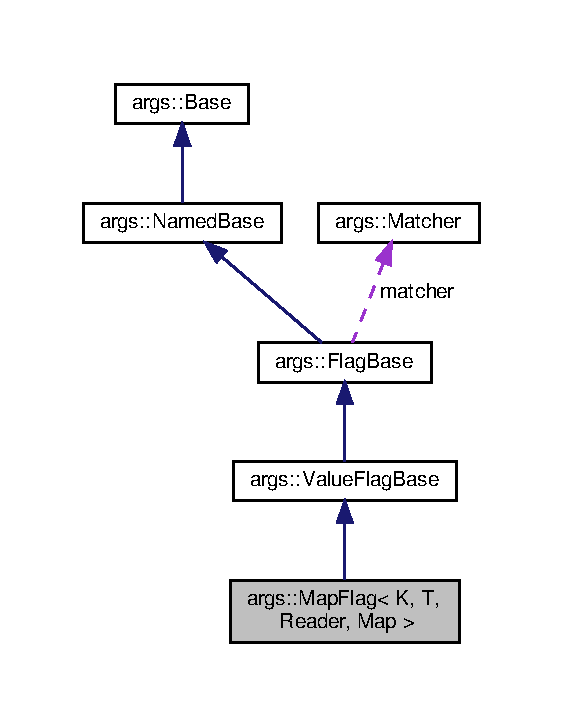
\includegraphics[width=270pt]{classargs_1_1_map_flag__coll__graph}
\end{center}
\end{figure}
\subsection*{Public Member Functions}
\begin{DoxyCompactItemize}
\item 
\hyperlink{classargs_1_1_map_flag_a36a375239e115d9923db2908330b4f75}{Map\+Flag} (\hyperlink{classargs_1_1_group}{Group} \&group\+\_\+, const std\+::string \&name\+\_\+, const std\+::string \&help\+\_\+, \hyperlink{classargs_1_1_matcher}{Matcher} \&\&matcher\+\_\+, const Map$<$ \hyperlink{cgal__test_8cpp_a891e241aa245ae63618f03737efba309}{K}, T $>$ \&map\+\_\+, const T \&default\+Value\+\_\+, \hyperlink{namespaceargs_aa530c0f95194aa275f49a5f299ac9e77}{Options} options\+\_\+)
\item 
\hyperlink{classargs_1_1_map_flag_a9e13951a327b382cfaa5caf8a0ecd9c9}{Map\+Flag} (\hyperlink{classargs_1_1_group}{Group} \&group\+\_\+, const std\+::string \&name\+\_\+, const std\+::string \&help\+\_\+, \hyperlink{classargs_1_1_matcher}{Matcher} \&\&matcher\+\_\+, const Map$<$ \hyperlink{cgal__test_8cpp_a891e241aa245ae63618f03737efba309}{K}, T $>$ \&map\+\_\+, const T \&default\+Value\+\_\+=T(), const bool extra\+Error\+\_\+=false)
\item 
\hyperlink{classargs_1_1_map_flag_a2da594dc6378fcaeca63e1dcb8b4d816}{Map\+Flag} (\hyperlink{classargs_1_1_group}{Group} \&group\+\_\+, const std\+::string \&name\+\_\+, const std\+::string \&help\+\_\+, \hyperlink{classargs_1_1_matcher}{Matcher} \&\&matcher\+\_\+, const Map$<$ \hyperlink{cgal__test_8cpp_a891e241aa245ae63618f03737efba309}{K}, T $>$ \&map\+\_\+, \hyperlink{namespaceargs_aa530c0f95194aa275f49a5f299ac9e77}{Options} options\+\_\+)
\item 
virtual \hyperlink{classargs_1_1_map_flag_a67afdb4326dcef52941a230fc188d54b}{$\sim$\+Map\+Flag} ()
\item 
virtual void \hyperlink{classargs_1_1_map_flag_a1f21b9227ab9b346b86f8533213a8272}{Parse\+Value} (const std\+::vector$<$ std\+::string $>$ \&values\+\_\+) override
\item 
T \& \hyperlink{classargs_1_1_map_flag_ad4f1db59b839e44157c5eba9b482b75c}{Get} () noexcept
\end{DoxyCompactItemize}
\subsection*{Protected Member Functions}
\begin{DoxyCompactItemize}
\item 
virtual std\+::string \hyperlink{classargs_1_1_map_flag_a7fe91b5ef6696b82aa8999884bbf727d}{Get\+Choices\+String} (const \hyperlink{structargs_1_1_help_params}{Help\+Params} \&) const override
\end{DoxyCompactItemize}
\subsection*{Additional Inherited Members}


\subsection{Detailed Description}
\subsubsection*{template$<$typename K, typename T, typename Reader = Value\+Reader, template$<$ typename... $>$ class Map = std\+::unordered\+\_\+map$>$\newline
class args\+::\+Map\+Flag$<$ K, T, Reader, Map $>$}

A mapping value flag class


\begin{DoxyTemplParams}{Template Parameters}
{\em K} & the type to extract the argument as \\
\hline
{\em T} & the type to store the result as \\
\hline
{\em Reader} & The functor type used to read the argument, taking the name, value, and destination reference with operator(), and returning a bool (if A\+R\+G\+S\+\_\+\+N\+O\+E\+X\+C\+E\+PT is defined) \\
\hline
{\em Map} & The Map type. Should operate like std\+::map or std\+::unordered\+\_\+map \\
\hline
\end{DoxyTemplParams}


\subsection{Constructor \& Destructor Documentation}
\mbox{\Hypertarget{classargs_1_1_map_flag_a36a375239e115d9923db2908330b4f75}\label{classargs_1_1_map_flag_a36a375239e115d9923db2908330b4f75}} 
\index{args\+::\+Map\+Flag@{args\+::\+Map\+Flag}!Map\+Flag@{Map\+Flag}}
\index{Map\+Flag@{Map\+Flag}!args\+::\+Map\+Flag@{args\+::\+Map\+Flag}}
\subsubsection{\texorpdfstring{Map\+Flag()}{MapFlag()}\hspace{0.1cm}{\footnotesize\ttfamily [1/3]}}
{\footnotesize\ttfamily template$<$typename K , typename T , typename Reader  = Value\+Reader, template$<$ typename... $>$ class Map = std\+::unordered\+\_\+map$>$ \\
\hyperlink{classargs_1_1_map_flag}{args\+::\+Map\+Flag}$<$ \hyperlink{cgal__test_8cpp_a891e241aa245ae63618f03737efba309}{K}, T, Reader, Map $>$\+::\hyperlink{classargs_1_1_map_flag}{Map\+Flag} (\begin{DoxyParamCaption}\item[{\hyperlink{classargs_1_1_group}{Group} \&}]{group\+\_\+,  }\item[{const std\+::string \&}]{name\+\_\+,  }\item[{const std\+::string \&}]{help\+\_\+,  }\item[{\hyperlink{classargs_1_1_matcher}{Matcher} \&\&}]{matcher\+\_\+,  }\item[{const Map$<$ \hyperlink{cgal__test_8cpp_a891e241aa245ae63618f03737efba309}{K}, T $>$ \&}]{map\+\_\+,  }\item[{const T \&}]{default\+Value\+\_\+,  }\item[{\hyperlink{namespaceargs_aa530c0f95194aa275f49a5f299ac9e77}{Options}}]{options\+\_\+ }\end{DoxyParamCaption})\hspace{0.3cm}{\ttfamily [inline]}}

\mbox{\Hypertarget{classargs_1_1_map_flag_a9e13951a327b382cfaa5caf8a0ecd9c9}\label{classargs_1_1_map_flag_a9e13951a327b382cfaa5caf8a0ecd9c9}} 
\index{args\+::\+Map\+Flag@{args\+::\+Map\+Flag}!Map\+Flag@{Map\+Flag}}
\index{Map\+Flag@{Map\+Flag}!args\+::\+Map\+Flag@{args\+::\+Map\+Flag}}
\subsubsection{\texorpdfstring{Map\+Flag()}{MapFlag()}\hspace{0.1cm}{\footnotesize\ttfamily [2/3]}}
{\footnotesize\ttfamily template$<$typename K , typename T , typename Reader  = Value\+Reader, template$<$ typename... $>$ class Map = std\+::unordered\+\_\+map$>$ \\
\hyperlink{classargs_1_1_map_flag}{args\+::\+Map\+Flag}$<$ \hyperlink{cgal__test_8cpp_a891e241aa245ae63618f03737efba309}{K}, T, Reader, Map $>$\+::\hyperlink{classargs_1_1_map_flag}{Map\+Flag} (\begin{DoxyParamCaption}\item[{\hyperlink{classargs_1_1_group}{Group} \&}]{group\+\_\+,  }\item[{const std\+::string \&}]{name\+\_\+,  }\item[{const std\+::string \&}]{help\+\_\+,  }\item[{\hyperlink{classargs_1_1_matcher}{Matcher} \&\&}]{matcher\+\_\+,  }\item[{const Map$<$ \hyperlink{cgal__test_8cpp_a891e241aa245ae63618f03737efba309}{K}, T $>$ \&}]{map\+\_\+,  }\item[{const T \&}]{default\+Value\+\_\+ = {\ttfamily T()},  }\item[{const bool}]{extra\+Error\+\_\+ = {\ttfamily false} }\end{DoxyParamCaption})\hspace{0.3cm}{\ttfamily [inline]}}

\mbox{\Hypertarget{classargs_1_1_map_flag_a2da594dc6378fcaeca63e1dcb8b4d816}\label{classargs_1_1_map_flag_a2da594dc6378fcaeca63e1dcb8b4d816}} 
\index{args\+::\+Map\+Flag@{args\+::\+Map\+Flag}!Map\+Flag@{Map\+Flag}}
\index{Map\+Flag@{Map\+Flag}!args\+::\+Map\+Flag@{args\+::\+Map\+Flag}}
\subsubsection{\texorpdfstring{Map\+Flag()}{MapFlag()}\hspace{0.1cm}{\footnotesize\ttfamily [3/3]}}
{\footnotesize\ttfamily template$<$typename K , typename T , typename Reader  = Value\+Reader, template$<$ typename... $>$ class Map = std\+::unordered\+\_\+map$>$ \\
\hyperlink{classargs_1_1_map_flag}{args\+::\+Map\+Flag}$<$ \hyperlink{cgal__test_8cpp_a891e241aa245ae63618f03737efba309}{K}, T, Reader, Map $>$\+::\hyperlink{classargs_1_1_map_flag}{Map\+Flag} (\begin{DoxyParamCaption}\item[{\hyperlink{classargs_1_1_group}{Group} \&}]{group\+\_\+,  }\item[{const std\+::string \&}]{name\+\_\+,  }\item[{const std\+::string \&}]{help\+\_\+,  }\item[{\hyperlink{classargs_1_1_matcher}{Matcher} \&\&}]{matcher\+\_\+,  }\item[{const Map$<$ \hyperlink{cgal__test_8cpp_a891e241aa245ae63618f03737efba309}{K}, T $>$ \&}]{map\+\_\+,  }\item[{\hyperlink{namespaceargs_aa530c0f95194aa275f49a5f299ac9e77}{Options}}]{options\+\_\+ }\end{DoxyParamCaption})\hspace{0.3cm}{\ttfamily [inline]}}

\mbox{\Hypertarget{classargs_1_1_map_flag_a67afdb4326dcef52941a230fc188d54b}\label{classargs_1_1_map_flag_a67afdb4326dcef52941a230fc188d54b}} 
\index{args\+::\+Map\+Flag@{args\+::\+Map\+Flag}!````~Map\+Flag@{$\sim$\+Map\+Flag}}
\index{````~Map\+Flag@{$\sim$\+Map\+Flag}!args\+::\+Map\+Flag@{args\+::\+Map\+Flag}}
\subsubsection{\texorpdfstring{$\sim$\+Map\+Flag()}{~MapFlag()}}
{\footnotesize\ttfamily template$<$typename K , typename T , typename Reader  = Value\+Reader, template$<$ typename... $>$ class Map = std\+::unordered\+\_\+map$>$ \\
virtual \hyperlink{classargs_1_1_map_flag}{args\+::\+Map\+Flag}$<$ \hyperlink{cgal__test_8cpp_a891e241aa245ae63618f03737efba309}{K}, T, Reader, Map $>$\+::$\sim$\hyperlink{classargs_1_1_map_flag}{Map\+Flag} (\begin{DoxyParamCaption}{ }\end{DoxyParamCaption})\hspace{0.3cm}{\ttfamily [inline]}, {\ttfamily [virtual]}}



\subsection{Member Function Documentation}
\mbox{\Hypertarget{classargs_1_1_map_flag_ad4f1db59b839e44157c5eba9b482b75c}\label{classargs_1_1_map_flag_ad4f1db59b839e44157c5eba9b482b75c}} 
\index{args\+::\+Map\+Flag@{args\+::\+Map\+Flag}!Get@{Get}}
\index{Get@{Get}!args\+::\+Map\+Flag@{args\+::\+Map\+Flag}}
\subsubsection{\texorpdfstring{Get()}{Get()}}
{\footnotesize\ttfamily template$<$typename K , typename T , typename Reader  = Value\+Reader, template$<$ typename... $>$ class Map = std\+::unordered\+\_\+map$>$ \\
T\& \hyperlink{classargs_1_1_map_flag}{args\+::\+Map\+Flag}$<$ \hyperlink{cgal__test_8cpp_a891e241aa245ae63618f03737efba309}{K}, T, Reader, Map $>$\+::Get (\begin{DoxyParamCaption}{ }\end{DoxyParamCaption})\hspace{0.3cm}{\ttfamily [inline]}, {\ttfamily [noexcept]}}

Get the value \mbox{\Hypertarget{classargs_1_1_map_flag_a7fe91b5ef6696b82aa8999884bbf727d}\label{classargs_1_1_map_flag_a7fe91b5ef6696b82aa8999884bbf727d}} 
\index{args\+::\+Map\+Flag@{args\+::\+Map\+Flag}!Get\+Choices\+String@{Get\+Choices\+String}}
\index{Get\+Choices\+String@{Get\+Choices\+String}!args\+::\+Map\+Flag@{args\+::\+Map\+Flag}}
\subsubsection{\texorpdfstring{Get\+Choices\+String()}{GetChoicesString()}}
{\footnotesize\ttfamily template$<$typename K , typename T , typename Reader  = Value\+Reader, template$<$ typename... $>$ class Map = std\+::unordered\+\_\+map$>$ \\
virtual std\+::string \hyperlink{classargs_1_1_map_flag}{args\+::\+Map\+Flag}$<$ \hyperlink{cgal__test_8cpp_a891e241aa245ae63618f03737efba309}{K}, T, Reader, Map $>$\+::Get\+Choices\+String (\begin{DoxyParamCaption}\item[{const \hyperlink{structargs_1_1_help_params}{Help\+Params} \&}]{ }\end{DoxyParamCaption}) const\hspace{0.3cm}{\ttfamily [inline]}, {\ttfamily [override]}, {\ttfamily [protected]}, {\ttfamily [virtual]}}



Reimplemented from \hyperlink{classargs_1_1_named_base_aa9104a04001d10c5732a5feb01204cf7}{args\+::\+Named\+Base}.

\mbox{\Hypertarget{classargs_1_1_map_flag_a1f21b9227ab9b346b86f8533213a8272}\label{classargs_1_1_map_flag_a1f21b9227ab9b346b86f8533213a8272}} 
\index{args\+::\+Map\+Flag@{args\+::\+Map\+Flag}!Parse\+Value@{Parse\+Value}}
\index{Parse\+Value@{Parse\+Value}!args\+::\+Map\+Flag@{args\+::\+Map\+Flag}}
\subsubsection{\texorpdfstring{Parse\+Value()}{ParseValue()}}
{\footnotesize\ttfamily template$<$typename K , typename T , typename Reader  = Value\+Reader, template$<$ typename... $>$ class Map = std\+::unordered\+\_\+map$>$ \\
virtual void \hyperlink{classargs_1_1_map_flag}{args\+::\+Map\+Flag}$<$ \hyperlink{cgal__test_8cpp_a891e241aa245ae63618f03737efba309}{K}, T, Reader, Map $>$\+::Parse\+Value (\begin{DoxyParamCaption}\item[{const std\+::vector$<$ std\+::string $>$ \&}]{value }\end{DoxyParamCaption})\hspace{0.3cm}{\ttfamily [inline]}, {\ttfamily [override]}, {\ttfamily [virtual]}}

Parse values of this option.


\begin{DoxyParams}{Parameters}
{\em value} & Vector of values. It\textquotesingle{}s size must be in \hyperlink{classargs_1_1_value_flag_base_a96a10bfb949ad175dcf2ffba6a6ec3b6}{Number\+Of\+Arguments()} interval. \\
\hline
\end{DoxyParams}


Implements \hyperlink{classargs_1_1_flag_base_a3421d9a595c9426dc73f62604cdee84f}{args\+::\+Flag\+Base}.



The documentation for this class was generated from the following file\+:\begin{DoxyCompactItemize}
\item 
/home/cappelletto/github/self/landing\+\_\+area\+\_\+detector/external/\hyperlink{args_8hxx}{args.\+hxx}\end{DoxyCompactItemize}

\hypertarget{classargs_1_1_map_flag_list}{}\section{args\+:\+:Map\+Flag\+List$<$ K, T, List, Reader, Map $>$ Class Template Reference}
\label{classargs_1_1_map_flag_list}\index{args\+::\+Map\+Flag\+List$<$ K, T, List, Reader, Map $>$@{args\+::\+Map\+Flag\+List$<$ K, T, List, Reader, Map $>$}}


{\ttfamily \#include $<$args.\+hxx$>$}



Inheritance diagram for args\+:\+:Map\+Flag\+List$<$ K, T, List, Reader, Map $>$\+:\nopagebreak
\begin{figure}[H]
\begin{center}
\leavevmode
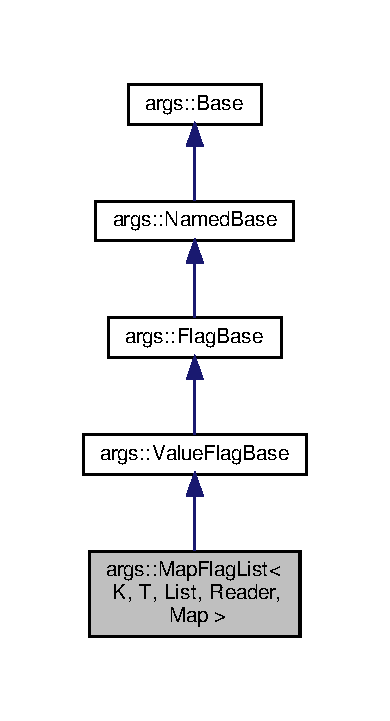
\includegraphics[width=187pt]{classargs_1_1_map_flag_list__inherit__graph}
\end{center}
\end{figure}


Collaboration diagram for args\+:\+:Map\+Flag\+List$<$ K, T, List, Reader, Map $>$\+:\nopagebreak
\begin{figure}[H]
\begin{center}
\leavevmode
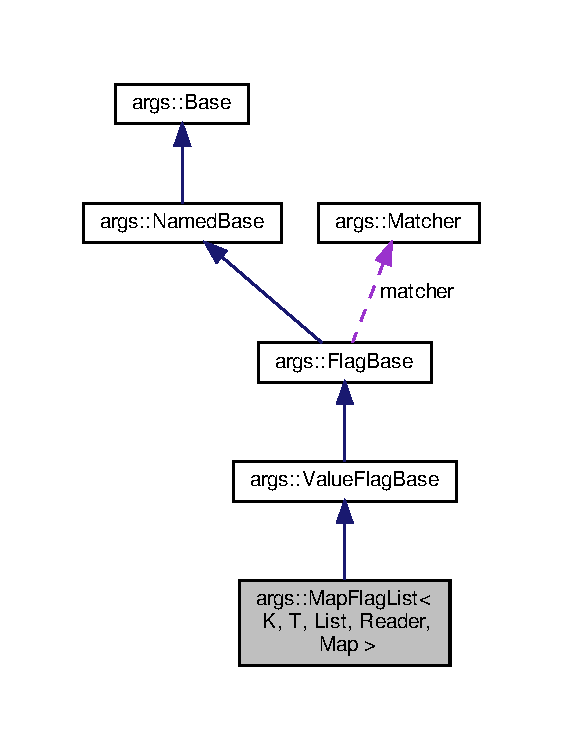
\includegraphics[width=270pt]{classargs_1_1_map_flag_list__coll__graph}
\end{center}
\end{figure}
\subsection*{Public Types}
\begin{DoxyCompactItemize}
\item 
typedef T \hyperlink{classargs_1_1_map_flag_list_a6c8d512f511bdcfac07e0394ca187d67}{value\+\_\+type}
\item 
typedef Container\+::allocator\+\_\+type \hyperlink{classargs_1_1_map_flag_list_a4f098b2b16c4c3ffc86a4e7bcef62068}{allocator\+\_\+type}
\item 
typedef Container\+::pointer \hyperlink{classargs_1_1_map_flag_list_a955d68bb97928f8292c5401810852067}{pointer}
\item 
typedef Container\+::const\+\_\+pointer \hyperlink{classargs_1_1_map_flag_list_a7dff9e884a42029fc9f5bd0fcbfb12c3}{const\+\_\+pointer}
\item 
typedef T \& \hyperlink{classargs_1_1_map_flag_list_a64534f886c974afc71a57134e95cab12}{reference}
\item 
typedef const T \& \hyperlink{classargs_1_1_map_flag_list_a68a39fcca6b7b4937d1a04c21b9749e5}{const\+\_\+reference}
\item 
typedef Container\+::size\+\_\+type \hyperlink{classargs_1_1_map_flag_list_aad04984bb8472e997a4145620b88ffa5}{size\+\_\+type}
\item 
typedef Container\+::difference\+\_\+type \hyperlink{classargs_1_1_map_flag_list_a704d125e630642ceb306b88b2059ec47}{difference\+\_\+type}
\item 
typedef Container\+::iterator \hyperlink{classargs_1_1_map_flag_list_a73b7f3d1f8e2dc8776c195c9d1b66d34}{iterator}
\item 
typedef Container\+::const\+\_\+iterator \hyperlink{classargs_1_1_map_flag_list_a6b59eb2e45bf0e576d01b902f3c7a0d7}{const\+\_\+iterator}
\item 
typedef std\+::reverse\+\_\+iterator$<$ \hyperlink{classargs_1_1_map_flag_list_a73b7f3d1f8e2dc8776c195c9d1b66d34}{iterator} $>$ \hyperlink{classargs_1_1_map_flag_list_aa7c8974f4f3d7b51ab883967b665f52f}{reverse\+\_\+iterator}
\item 
typedef std\+::reverse\+\_\+iterator$<$ \hyperlink{classargs_1_1_map_flag_list_a6b59eb2e45bf0e576d01b902f3c7a0d7}{const\+\_\+iterator} $>$ \hyperlink{classargs_1_1_map_flag_list_ad2ab0776f807550d0f4c86bb885a6a0c}{const\+\_\+reverse\+\_\+iterator}
\end{DoxyCompactItemize}
\subsection*{Public Member Functions}
\begin{DoxyCompactItemize}
\item 
\hyperlink{classargs_1_1_map_flag_list_a8a7d44c211928287ced52601a30268c9}{Map\+Flag\+List} (\hyperlink{classargs_1_1_group}{Group} \&group\+\_\+, const std\+::string \&name\+\_\+, const std\+::string \&help\+\_\+, \hyperlink{classargs_1_1_matcher}{Matcher} \&\&matcher\+\_\+, const Map$<$ \hyperlink{cgal__test_8cpp_a891e241aa245ae63618f03737efba309}{K}, T $>$ \&map\+\_\+, const Container \&default\+Values\+\_\+=Container())
\item 
virtual \hyperlink{classargs_1_1_map_flag_list_a8799bf86215d5a166efc57e1c8b512e2}{$\sim$\+Map\+Flag\+List} ()
\item 
virtual void \hyperlink{classargs_1_1_map_flag_list_af37b4d7e420eabf62bd8dacafa86419c}{Parse\+Value} (const std\+::vector$<$ std\+::string $>$ \&values\+\_\+) override
\item 
Container \& \hyperlink{classargs_1_1_map_flag_list_ada0e7eb9bec54ed768bfa206af4b3bb9}{Get} () noexcept
\item 
virtual std\+::string \hyperlink{classargs_1_1_map_flag_list_a1703584ba7b36c5e15aa375eae23903c}{Name} () const override
\item 
virtual void \hyperlink{classargs_1_1_map_flag_list_a993bb59f57246e246edbd6ac3fc048eb}{Reset} () noexcept override
\item 
\hyperlink{classargs_1_1_map_flag_list_a73b7f3d1f8e2dc8776c195c9d1b66d34}{iterator} \hyperlink{classargs_1_1_map_flag_list_a21d879d48f9adf298b1dd824c5cb2e1b}{begin} () noexcept
\item 
\hyperlink{classargs_1_1_map_flag_list_a6b59eb2e45bf0e576d01b902f3c7a0d7}{const\+\_\+iterator} \hyperlink{classargs_1_1_map_flag_list_a8592b905d9930af771a904ddd02f185f}{begin} () const noexcept
\item 
\hyperlink{classargs_1_1_map_flag_list_a6b59eb2e45bf0e576d01b902f3c7a0d7}{const\+\_\+iterator} \hyperlink{classargs_1_1_map_flag_list_ae2a91b86b914cfcb9bdf1d855d50f7e2}{cbegin} () const noexcept
\item 
\hyperlink{classargs_1_1_map_flag_list_a73b7f3d1f8e2dc8776c195c9d1b66d34}{iterator} \hyperlink{classargs_1_1_map_flag_list_a53c9c5bf837f5b27b72a599069a87884}{end} () noexcept
\item 
\hyperlink{classargs_1_1_map_flag_list_a6b59eb2e45bf0e576d01b902f3c7a0d7}{const\+\_\+iterator} \hyperlink{classargs_1_1_map_flag_list_ac6c7c678cc3680a6df82b972aeaee561}{end} () const noexcept
\item 
\hyperlink{classargs_1_1_map_flag_list_a6b59eb2e45bf0e576d01b902f3c7a0d7}{const\+\_\+iterator} \hyperlink{classargs_1_1_map_flag_list_a565f9a371dc12dcdb4665057cf465709}{cend} () const noexcept
\end{DoxyCompactItemize}
\subsection*{Additional Inherited Members}


\subsection{Detailed Description}
\subsubsection*{template$<$typename K, typename T, template$<$ typename... $>$ class List = std\+::vector, typename Reader = Value\+Reader, template$<$ typename... $>$ class Map = std\+::unordered\+\_\+map$>$\newline
class args\+::\+Map\+Flag\+List$<$ K, T, List, Reader, Map $>$}

A mapping value flag list class


\begin{DoxyTemplParams}{Template Parameters}
{\em K} & the type to extract the argument as \\
\hline
{\em T} & the type to store the result as \\
\hline
{\em List} & the list type that houses the values \\
\hline
{\em Reader} & The functor type used to read the argument, taking the name, value, and destination reference with operator(), and returning a bool (if A\+R\+G\+S\+\_\+\+N\+O\+E\+X\+C\+E\+PT is defined) \\
\hline
{\em Map} & The Map type. Should operate like std\+::map or std\+::unordered\+\_\+map \\
\hline
\end{DoxyTemplParams}


\subsection{Member Typedef Documentation}
\mbox{\Hypertarget{classargs_1_1_map_flag_list_a4f098b2b16c4c3ffc86a4e7bcef62068}\label{classargs_1_1_map_flag_list_a4f098b2b16c4c3ffc86a4e7bcef62068}} 
\index{args\+::\+Map\+Flag\+List@{args\+::\+Map\+Flag\+List}!allocator\+\_\+type@{allocator\+\_\+type}}
\index{allocator\+\_\+type@{allocator\+\_\+type}!args\+::\+Map\+Flag\+List@{args\+::\+Map\+Flag\+List}}
\subsubsection{\texorpdfstring{allocator\+\_\+type}{allocator\_type}}
{\footnotesize\ttfamily template$<$typename K , typename T , template$<$ typename... $>$ class List = std\+::vector, typename Reader  = Value\+Reader, template$<$ typename... $>$ class Map = std\+::unordered\+\_\+map$>$ \\
typedef Container\+::allocator\+\_\+type \hyperlink{classargs_1_1_map_flag_list}{args\+::\+Map\+Flag\+List}$<$ \hyperlink{cgal__test_8cpp_a891e241aa245ae63618f03737efba309}{K}, T, List, Reader, Map $>$\+::\hyperlink{classargs_1_1_map_flag_list_a4f098b2b16c4c3ffc86a4e7bcef62068}{allocator\+\_\+type}}

\mbox{\Hypertarget{classargs_1_1_map_flag_list_a6b59eb2e45bf0e576d01b902f3c7a0d7}\label{classargs_1_1_map_flag_list_a6b59eb2e45bf0e576d01b902f3c7a0d7}} 
\index{args\+::\+Map\+Flag\+List@{args\+::\+Map\+Flag\+List}!const\+\_\+iterator@{const\+\_\+iterator}}
\index{const\+\_\+iterator@{const\+\_\+iterator}!args\+::\+Map\+Flag\+List@{args\+::\+Map\+Flag\+List}}
\subsubsection{\texorpdfstring{const\+\_\+iterator}{const\_iterator}}
{\footnotesize\ttfamily template$<$typename K , typename T , template$<$ typename... $>$ class List = std\+::vector, typename Reader  = Value\+Reader, template$<$ typename... $>$ class Map = std\+::unordered\+\_\+map$>$ \\
typedef Container\+::const\+\_\+iterator \hyperlink{classargs_1_1_map_flag_list}{args\+::\+Map\+Flag\+List}$<$ \hyperlink{cgal__test_8cpp_a891e241aa245ae63618f03737efba309}{K}, T, List, Reader, Map $>$\+::\hyperlink{classargs_1_1_map_flag_list_a6b59eb2e45bf0e576d01b902f3c7a0d7}{const\+\_\+iterator}}

\mbox{\Hypertarget{classargs_1_1_map_flag_list_a7dff9e884a42029fc9f5bd0fcbfb12c3}\label{classargs_1_1_map_flag_list_a7dff9e884a42029fc9f5bd0fcbfb12c3}} 
\index{args\+::\+Map\+Flag\+List@{args\+::\+Map\+Flag\+List}!const\+\_\+pointer@{const\+\_\+pointer}}
\index{const\+\_\+pointer@{const\+\_\+pointer}!args\+::\+Map\+Flag\+List@{args\+::\+Map\+Flag\+List}}
\subsubsection{\texorpdfstring{const\+\_\+pointer}{const\_pointer}}
{\footnotesize\ttfamily template$<$typename K , typename T , template$<$ typename... $>$ class List = std\+::vector, typename Reader  = Value\+Reader, template$<$ typename... $>$ class Map = std\+::unordered\+\_\+map$>$ \\
typedef Container\+::const\+\_\+pointer \hyperlink{classargs_1_1_map_flag_list}{args\+::\+Map\+Flag\+List}$<$ \hyperlink{cgal__test_8cpp_a891e241aa245ae63618f03737efba309}{K}, T, List, Reader, Map $>$\+::\hyperlink{classargs_1_1_map_flag_list_a7dff9e884a42029fc9f5bd0fcbfb12c3}{const\+\_\+pointer}}

\mbox{\Hypertarget{classargs_1_1_map_flag_list_a68a39fcca6b7b4937d1a04c21b9749e5}\label{classargs_1_1_map_flag_list_a68a39fcca6b7b4937d1a04c21b9749e5}} 
\index{args\+::\+Map\+Flag\+List@{args\+::\+Map\+Flag\+List}!const\+\_\+reference@{const\+\_\+reference}}
\index{const\+\_\+reference@{const\+\_\+reference}!args\+::\+Map\+Flag\+List@{args\+::\+Map\+Flag\+List}}
\subsubsection{\texorpdfstring{const\+\_\+reference}{const\_reference}}
{\footnotesize\ttfamily template$<$typename K , typename T , template$<$ typename... $>$ class List = std\+::vector, typename Reader  = Value\+Reader, template$<$ typename... $>$ class Map = std\+::unordered\+\_\+map$>$ \\
typedef const T\& \hyperlink{classargs_1_1_map_flag_list}{args\+::\+Map\+Flag\+List}$<$ \hyperlink{cgal__test_8cpp_a891e241aa245ae63618f03737efba309}{K}, T, List, Reader, Map $>$\+::\hyperlink{classargs_1_1_map_flag_list_a68a39fcca6b7b4937d1a04c21b9749e5}{const\+\_\+reference}}

\mbox{\Hypertarget{classargs_1_1_map_flag_list_ad2ab0776f807550d0f4c86bb885a6a0c}\label{classargs_1_1_map_flag_list_ad2ab0776f807550d0f4c86bb885a6a0c}} 
\index{args\+::\+Map\+Flag\+List@{args\+::\+Map\+Flag\+List}!const\+\_\+reverse\+\_\+iterator@{const\+\_\+reverse\+\_\+iterator}}
\index{const\+\_\+reverse\+\_\+iterator@{const\+\_\+reverse\+\_\+iterator}!args\+::\+Map\+Flag\+List@{args\+::\+Map\+Flag\+List}}
\subsubsection{\texorpdfstring{const\+\_\+reverse\+\_\+iterator}{const\_reverse\_iterator}}
{\footnotesize\ttfamily template$<$typename K , typename T , template$<$ typename... $>$ class List = std\+::vector, typename Reader  = Value\+Reader, template$<$ typename... $>$ class Map = std\+::unordered\+\_\+map$>$ \\
typedef std\+::reverse\+\_\+iterator$<$\hyperlink{classargs_1_1_map_flag_list_a6b59eb2e45bf0e576d01b902f3c7a0d7}{const\+\_\+iterator}$>$ \hyperlink{classargs_1_1_map_flag_list}{args\+::\+Map\+Flag\+List}$<$ \hyperlink{cgal__test_8cpp_a891e241aa245ae63618f03737efba309}{K}, T, List, Reader, Map $>$\+::\hyperlink{classargs_1_1_map_flag_list_ad2ab0776f807550d0f4c86bb885a6a0c}{const\+\_\+reverse\+\_\+iterator}}

\mbox{\Hypertarget{classargs_1_1_map_flag_list_a704d125e630642ceb306b88b2059ec47}\label{classargs_1_1_map_flag_list_a704d125e630642ceb306b88b2059ec47}} 
\index{args\+::\+Map\+Flag\+List@{args\+::\+Map\+Flag\+List}!difference\+\_\+type@{difference\+\_\+type}}
\index{difference\+\_\+type@{difference\+\_\+type}!args\+::\+Map\+Flag\+List@{args\+::\+Map\+Flag\+List}}
\subsubsection{\texorpdfstring{difference\+\_\+type}{difference\_type}}
{\footnotesize\ttfamily template$<$typename K , typename T , template$<$ typename... $>$ class List = std\+::vector, typename Reader  = Value\+Reader, template$<$ typename... $>$ class Map = std\+::unordered\+\_\+map$>$ \\
typedef Container\+::difference\+\_\+type \hyperlink{classargs_1_1_map_flag_list}{args\+::\+Map\+Flag\+List}$<$ \hyperlink{cgal__test_8cpp_a891e241aa245ae63618f03737efba309}{K}, T, List, Reader, Map $>$\+::\hyperlink{classargs_1_1_map_flag_list_a704d125e630642ceb306b88b2059ec47}{difference\+\_\+type}}

\mbox{\Hypertarget{classargs_1_1_map_flag_list_a73b7f3d1f8e2dc8776c195c9d1b66d34}\label{classargs_1_1_map_flag_list_a73b7f3d1f8e2dc8776c195c9d1b66d34}} 
\index{args\+::\+Map\+Flag\+List@{args\+::\+Map\+Flag\+List}!iterator@{iterator}}
\index{iterator@{iterator}!args\+::\+Map\+Flag\+List@{args\+::\+Map\+Flag\+List}}
\subsubsection{\texorpdfstring{iterator}{iterator}}
{\footnotesize\ttfamily template$<$typename K , typename T , template$<$ typename... $>$ class List = std\+::vector, typename Reader  = Value\+Reader, template$<$ typename... $>$ class Map = std\+::unordered\+\_\+map$>$ \\
typedef Container\+::iterator \hyperlink{classargs_1_1_map_flag_list}{args\+::\+Map\+Flag\+List}$<$ \hyperlink{cgal__test_8cpp_a891e241aa245ae63618f03737efba309}{K}, T, List, Reader, Map $>$\+::\hyperlink{classargs_1_1_map_flag_list_a73b7f3d1f8e2dc8776c195c9d1b66d34}{iterator}}

\mbox{\Hypertarget{classargs_1_1_map_flag_list_a955d68bb97928f8292c5401810852067}\label{classargs_1_1_map_flag_list_a955d68bb97928f8292c5401810852067}} 
\index{args\+::\+Map\+Flag\+List@{args\+::\+Map\+Flag\+List}!pointer@{pointer}}
\index{pointer@{pointer}!args\+::\+Map\+Flag\+List@{args\+::\+Map\+Flag\+List}}
\subsubsection{\texorpdfstring{pointer}{pointer}}
{\footnotesize\ttfamily template$<$typename K , typename T , template$<$ typename... $>$ class List = std\+::vector, typename Reader  = Value\+Reader, template$<$ typename... $>$ class Map = std\+::unordered\+\_\+map$>$ \\
typedef Container\+::pointer \hyperlink{classargs_1_1_map_flag_list}{args\+::\+Map\+Flag\+List}$<$ \hyperlink{cgal__test_8cpp_a891e241aa245ae63618f03737efba309}{K}, T, List, Reader, Map $>$\+::\hyperlink{classargs_1_1_map_flag_list_a955d68bb97928f8292c5401810852067}{pointer}}

\mbox{\Hypertarget{classargs_1_1_map_flag_list_a64534f886c974afc71a57134e95cab12}\label{classargs_1_1_map_flag_list_a64534f886c974afc71a57134e95cab12}} 
\index{args\+::\+Map\+Flag\+List@{args\+::\+Map\+Flag\+List}!reference@{reference}}
\index{reference@{reference}!args\+::\+Map\+Flag\+List@{args\+::\+Map\+Flag\+List}}
\subsubsection{\texorpdfstring{reference}{reference}}
{\footnotesize\ttfamily template$<$typename K , typename T , template$<$ typename... $>$ class List = std\+::vector, typename Reader  = Value\+Reader, template$<$ typename... $>$ class Map = std\+::unordered\+\_\+map$>$ \\
typedef T\& \hyperlink{classargs_1_1_map_flag_list}{args\+::\+Map\+Flag\+List}$<$ \hyperlink{cgal__test_8cpp_a891e241aa245ae63618f03737efba309}{K}, T, List, Reader, Map $>$\+::\hyperlink{classargs_1_1_map_flag_list_a64534f886c974afc71a57134e95cab12}{reference}}

\mbox{\Hypertarget{classargs_1_1_map_flag_list_aa7c8974f4f3d7b51ab883967b665f52f}\label{classargs_1_1_map_flag_list_aa7c8974f4f3d7b51ab883967b665f52f}} 
\index{args\+::\+Map\+Flag\+List@{args\+::\+Map\+Flag\+List}!reverse\+\_\+iterator@{reverse\+\_\+iterator}}
\index{reverse\+\_\+iterator@{reverse\+\_\+iterator}!args\+::\+Map\+Flag\+List@{args\+::\+Map\+Flag\+List}}
\subsubsection{\texorpdfstring{reverse\+\_\+iterator}{reverse\_iterator}}
{\footnotesize\ttfamily template$<$typename K , typename T , template$<$ typename... $>$ class List = std\+::vector, typename Reader  = Value\+Reader, template$<$ typename... $>$ class Map = std\+::unordered\+\_\+map$>$ \\
typedef std\+::reverse\+\_\+iterator$<$\hyperlink{classargs_1_1_map_flag_list_a73b7f3d1f8e2dc8776c195c9d1b66d34}{iterator}$>$ \hyperlink{classargs_1_1_map_flag_list}{args\+::\+Map\+Flag\+List}$<$ \hyperlink{cgal__test_8cpp_a891e241aa245ae63618f03737efba309}{K}, T, List, Reader, Map $>$\+::\hyperlink{classargs_1_1_map_flag_list_aa7c8974f4f3d7b51ab883967b665f52f}{reverse\+\_\+iterator}}

\mbox{\Hypertarget{classargs_1_1_map_flag_list_aad04984bb8472e997a4145620b88ffa5}\label{classargs_1_1_map_flag_list_aad04984bb8472e997a4145620b88ffa5}} 
\index{args\+::\+Map\+Flag\+List@{args\+::\+Map\+Flag\+List}!size\+\_\+type@{size\+\_\+type}}
\index{size\+\_\+type@{size\+\_\+type}!args\+::\+Map\+Flag\+List@{args\+::\+Map\+Flag\+List}}
\subsubsection{\texorpdfstring{size\+\_\+type}{size\_type}}
{\footnotesize\ttfamily template$<$typename K , typename T , template$<$ typename... $>$ class List = std\+::vector, typename Reader  = Value\+Reader, template$<$ typename... $>$ class Map = std\+::unordered\+\_\+map$>$ \\
typedef Container\+::size\+\_\+type \hyperlink{classargs_1_1_map_flag_list}{args\+::\+Map\+Flag\+List}$<$ \hyperlink{cgal__test_8cpp_a891e241aa245ae63618f03737efba309}{K}, T, List, Reader, Map $>$\+::\hyperlink{classargs_1_1_map_flag_list_aad04984bb8472e997a4145620b88ffa5}{size\+\_\+type}}

\mbox{\Hypertarget{classargs_1_1_map_flag_list_a6c8d512f511bdcfac07e0394ca187d67}\label{classargs_1_1_map_flag_list_a6c8d512f511bdcfac07e0394ca187d67}} 
\index{args\+::\+Map\+Flag\+List@{args\+::\+Map\+Flag\+List}!value\+\_\+type@{value\+\_\+type}}
\index{value\+\_\+type@{value\+\_\+type}!args\+::\+Map\+Flag\+List@{args\+::\+Map\+Flag\+List}}
\subsubsection{\texorpdfstring{value\+\_\+type}{value\_type}}
{\footnotesize\ttfamily template$<$typename K , typename T , template$<$ typename... $>$ class List = std\+::vector, typename Reader  = Value\+Reader, template$<$ typename... $>$ class Map = std\+::unordered\+\_\+map$>$ \\
typedef T \hyperlink{classargs_1_1_map_flag_list}{args\+::\+Map\+Flag\+List}$<$ \hyperlink{cgal__test_8cpp_a891e241aa245ae63618f03737efba309}{K}, T, List, Reader, Map $>$\+::\hyperlink{classargs_1_1_map_flag_list_a6c8d512f511bdcfac07e0394ca187d67}{value\+\_\+type}}



\subsection{Constructor \& Destructor Documentation}
\mbox{\Hypertarget{classargs_1_1_map_flag_list_a8a7d44c211928287ced52601a30268c9}\label{classargs_1_1_map_flag_list_a8a7d44c211928287ced52601a30268c9}} 
\index{args\+::\+Map\+Flag\+List@{args\+::\+Map\+Flag\+List}!Map\+Flag\+List@{Map\+Flag\+List}}
\index{Map\+Flag\+List@{Map\+Flag\+List}!args\+::\+Map\+Flag\+List@{args\+::\+Map\+Flag\+List}}
\subsubsection{\texorpdfstring{Map\+Flag\+List()}{MapFlagList()}}
{\footnotesize\ttfamily template$<$typename K , typename T , template$<$ typename... $>$ class List = std\+::vector, typename Reader  = Value\+Reader, template$<$ typename... $>$ class Map = std\+::unordered\+\_\+map$>$ \\
\hyperlink{classargs_1_1_map_flag_list}{args\+::\+Map\+Flag\+List}$<$ \hyperlink{cgal__test_8cpp_a891e241aa245ae63618f03737efba309}{K}, T, List, Reader, Map $>$\+::\hyperlink{classargs_1_1_map_flag_list}{Map\+Flag\+List} (\begin{DoxyParamCaption}\item[{\hyperlink{classargs_1_1_group}{Group} \&}]{group\+\_\+,  }\item[{const std\+::string \&}]{name\+\_\+,  }\item[{const std\+::string \&}]{help\+\_\+,  }\item[{\hyperlink{classargs_1_1_matcher}{Matcher} \&\&}]{matcher\+\_\+,  }\item[{const Map$<$ \hyperlink{cgal__test_8cpp_a891e241aa245ae63618f03737efba309}{K}, T $>$ \&}]{map\+\_\+,  }\item[{const Container \&}]{default\+Values\+\_\+ = {\ttfamily Container()} }\end{DoxyParamCaption})\hspace{0.3cm}{\ttfamily [inline]}}

\mbox{\Hypertarget{classargs_1_1_map_flag_list_a8799bf86215d5a166efc57e1c8b512e2}\label{classargs_1_1_map_flag_list_a8799bf86215d5a166efc57e1c8b512e2}} 
\index{args\+::\+Map\+Flag\+List@{args\+::\+Map\+Flag\+List}!````~Map\+Flag\+List@{$\sim$\+Map\+Flag\+List}}
\index{````~Map\+Flag\+List@{$\sim$\+Map\+Flag\+List}!args\+::\+Map\+Flag\+List@{args\+::\+Map\+Flag\+List}}
\subsubsection{\texorpdfstring{$\sim$\+Map\+Flag\+List()}{~MapFlagList()}}
{\footnotesize\ttfamily template$<$typename K , typename T , template$<$ typename... $>$ class List = std\+::vector, typename Reader  = Value\+Reader, template$<$ typename... $>$ class Map = std\+::unordered\+\_\+map$>$ \\
virtual \hyperlink{classargs_1_1_map_flag_list}{args\+::\+Map\+Flag\+List}$<$ \hyperlink{cgal__test_8cpp_a891e241aa245ae63618f03737efba309}{K}, T, List, Reader, Map $>$\+::$\sim$\hyperlink{classargs_1_1_map_flag_list}{Map\+Flag\+List} (\begin{DoxyParamCaption}{ }\end{DoxyParamCaption})\hspace{0.3cm}{\ttfamily [inline]}, {\ttfamily [virtual]}}



\subsection{Member Function Documentation}
\mbox{\Hypertarget{classargs_1_1_map_flag_list_a21d879d48f9adf298b1dd824c5cb2e1b}\label{classargs_1_1_map_flag_list_a21d879d48f9adf298b1dd824c5cb2e1b}} 
\index{args\+::\+Map\+Flag\+List@{args\+::\+Map\+Flag\+List}!begin@{begin}}
\index{begin@{begin}!args\+::\+Map\+Flag\+List@{args\+::\+Map\+Flag\+List}}
\subsubsection{\texorpdfstring{begin()}{begin()}\hspace{0.1cm}{\footnotesize\ttfamily [1/2]}}
{\footnotesize\ttfamily template$<$typename K , typename T , template$<$ typename... $>$ class List = std\+::vector, typename Reader  = Value\+Reader, template$<$ typename... $>$ class Map = std\+::unordered\+\_\+map$>$ \\
\hyperlink{classargs_1_1_map_flag_list_a73b7f3d1f8e2dc8776c195c9d1b66d34}{iterator} \hyperlink{classargs_1_1_map_flag_list}{args\+::\+Map\+Flag\+List}$<$ \hyperlink{cgal__test_8cpp_a891e241aa245ae63618f03737efba309}{K}, T, List, Reader, Map $>$\+::begin (\begin{DoxyParamCaption}{ }\end{DoxyParamCaption})\hspace{0.3cm}{\ttfamily [inline]}, {\ttfamily [noexcept]}}

\mbox{\Hypertarget{classargs_1_1_map_flag_list_a8592b905d9930af771a904ddd02f185f}\label{classargs_1_1_map_flag_list_a8592b905d9930af771a904ddd02f185f}} 
\index{args\+::\+Map\+Flag\+List@{args\+::\+Map\+Flag\+List}!begin@{begin}}
\index{begin@{begin}!args\+::\+Map\+Flag\+List@{args\+::\+Map\+Flag\+List}}
\subsubsection{\texorpdfstring{begin()}{begin()}\hspace{0.1cm}{\footnotesize\ttfamily [2/2]}}
{\footnotesize\ttfamily template$<$typename K , typename T , template$<$ typename... $>$ class List = std\+::vector, typename Reader  = Value\+Reader, template$<$ typename... $>$ class Map = std\+::unordered\+\_\+map$>$ \\
\hyperlink{classargs_1_1_map_flag_list_a6b59eb2e45bf0e576d01b902f3c7a0d7}{const\+\_\+iterator} \hyperlink{classargs_1_1_map_flag_list}{args\+::\+Map\+Flag\+List}$<$ \hyperlink{cgal__test_8cpp_a891e241aa245ae63618f03737efba309}{K}, T, List, Reader, Map $>$\+::begin (\begin{DoxyParamCaption}{ }\end{DoxyParamCaption}) const\hspace{0.3cm}{\ttfamily [inline]}, {\ttfamily [noexcept]}}

\mbox{\Hypertarget{classargs_1_1_map_flag_list_ae2a91b86b914cfcb9bdf1d855d50f7e2}\label{classargs_1_1_map_flag_list_ae2a91b86b914cfcb9bdf1d855d50f7e2}} 
\index{args\+::\+Map\+Flag\+List@{args\+::\+Map\+Flag\+List}!cbegin@{cbegin}}
\index{cbegin@{cbegin}!args\+::\+Map\+Flag\+List@{args\+::\+Map\+Flag\+List}}
\subsubsection{\texorpdfstring{cbegin()}{cbegin()}}
{\footnotesize\ttfamily template$<$typename K , typename T , template$<$ typename... $>$ class List = std\+::vector, typename Reader  = Value\+Reader, template$<$ typename... $>$ class Map = std\+::unordered\+\_\+map$>$ \\
\hyperlink{classargs_1_1_map_flag_list_a6b59eb2e45bf0e576d01b902f3c7a0d7}{const\+\_\+iterator} \hyperlink{classargs_1_1_map_flag_list}{args\+::\+Map\+Flag\+List}$<$ \hyperlink{cgal__test_8cpp_a891e241aa245ae63618f03737efba309}{K}, T, List, Reader, Map $>$\+::cbegin (\begin{DoxyParamCaption}{ }\end{DoxyParamCaption}) const\hspace{0.3cm}{\ttfamily [inline]}, {\ttfamily [noexcept]}}

\mbox{\Hypertarget{classargs_1_1_map_flag_list_a565f9a371dc12dcdb4665057cf465709}\label{classargs_1_1_map_flag_list_a565f9a371dc12dcdb4665057cf465709}} 
\index{args\+::\+Map\+Flag\+List@{args\+::\+Map\+Flag\+List}!cend@{cend}}
\index{cend@{cend}!args\+::\+Map\+Flag\+List@{args\+::\+Map\+Flag\+List}}
\subsubsection{\texorpdfstring{cend()}{cend()}}
{\footnotesize\ttfamily template$<$typename K , typename T , template$<$ typename... $>$ class List = std\+::vector, typename Reader  = Value\+Reader, template$<$ typename... $>$ class Map = std\+::unordered\+\_\+map$>$ \\
\hyperlink{classargs_1_1_map_flag_list_a6b59eb2e45bf0e576d01b902f3c7a0d7}{const\+\_\+iterator} \hyperlink{classargs_1_1_map_flag_list}{args\+::\+Map\+Flag\+List}$<$ \hyperlink{cgal__test_8cpp_a891e241aa245ae63618f03737efba309}{K}, T, List, Reader, Map $>$\+::cend (\begin{DoxyParamCaption}{ }\end{DoxyParamCaption}) const\hspace{0.3cm}{\ttfamily [inline]}, {\ttfamily [noexcept]}}

\mbox{\Hypertarget{classargs_1_1_map_flag_list_a53c9c5bf837f5b27b72a599069a87884}\label{classargs_1_1_map_flag_list_a53c9c5bf837f5b27b72a599069a87884}} 
\index{args\+::\+Map\+Flag\+List@{args\+::\+Map\+Flag\+List}!end@{end}}
\index{end@{end}!args\+::\+Map\+Flag\+List@{args\+::\+Map\+Flag\+List}}
\subsubsection{\texorpdfstring{end()}{end()}\hspace{0.1cm}{\footnotesize\ttfamily [1/2]}}
{\footnotesize\ttfamily template$<$typename K , typename T , template$<$ typename... $>$ class List = std\+::vector, typename Reader  = Value\+Reader, template$<$ typename... $>$ class Map = std\+::unordered\+\_\+map$>$ \\
\hyperlink{classargs_1_1_map_flag_list_a73b7f3d1f8e2dc8776c195c9d1b66d34}{iterator} \hyperlink{classargs_1_1_map_flag_list}{args\+::\+Map\+Flag\+List}$<$ \hyperlink{cgal__test_8cpp_a891e241aa245ae63618f03737efba309}{K}, T, List, Reader, Map $>$\+::end (\begin{DoxyParamCaption}{ }\end{DoxyParamCaption})\hspace{0.3cm}{\ttfamily [inline]}, {\ttfamily [noexcept]}}

\mbox{\Hypertarget{classargs_1_1_map_flag_list_ac6c7c678cc3680a6df82b972aeaee561}\label{classargs_1_1_map_flag_list_ac6c7c678cc3680a6df82b972aeaee561}} 
\index{args\+::\+Map\+Flag\+List@{args\+::\+Map\+Flag\+List}!end@{end}}
\index{end@{end}!args\+::\+Map\+Flag\+List@{args\+::\+Map\+Flag\+List}}
\subsubsection{\texorpdfstring{end()}{end()}\hspace{0.1cm}{\footnotesize\ttfamily [2/2]}}
{\footnotesize\ttfamily template$<$typename K , typename T , template$<$ typename... $>$ class List = std\+::vector, typename Reader  = Value\+Reader, template$<$ typename... $>$ class Map = std\+::unordered\+\_\+map$>$ \\
\hyperlink{classargs_1_1_map_flag_list_a6b59eb2e45bf0e576d01b902f3c7a0d7}{const\+\_\+iterator} \hyperlink{classargs_1_1_map_flag_list}{args\+::\+Map\+Flag\+List}$<$ \hyperlink{cgal__test_8cpp_a891e241aa245ae63618f03737efba309}{K}, T, List, Reader, Map $>$\+::end (\begin{DoxyParamCaption}{ }\end{DoxyParamCaption}) const\hspace{0.3cm}{\ttfamily [inline]}, {\ttfamily [noexcept]}}

\mbox{\Hypertarget{classargs_1_1_map_flag_list_ada0e7eb9bec54ed768bfa206af4b3bb9}\label{classargs_1_1_map_flag_list_ada0e7eb9bec54ed768bfa206af4b3bb9}} 
\index{args\+::\+Map\+Flag\+List@{args\+::\+Map\+Flag\+List}!Get@{Get}}
\index{Get@{Get}!args\+::\+Map\+Flag\+List@{args\+::\+Map\+Flag\+List}}
\subsubsection{\texorpdfstring{Get()}{Get()}}
{\footnotesize\ttfamily template$<$typename K , typename T , template$<$ typename... $>$ class List = std\+::vector, typename Reader  = Value\+Reader, template$<$ typename... $>$ class Map = std\+::unordered\+\_\+map$>$ \\
Container\& \hyperlink{classargs_1_1_map_flag_list}{args\+::\+Map\+Flag\+List}$<$ \hyperlink{cgal__test_8cpp_a891e241aa245ae63618f03737efba309}{K}, T, List, Reader, Map $>$\+::Get (\begin{DoxyParamCaption}{ }\end{DoxyParamCaption})\hspace{0.3cm}{\ttfamily [inline]}, {\ttfamily [noexcept]}}

Get the value \mbox{\Hypertarget{classargs_1_1_map_flag_list_a1703584ba7b36c5e15aa375eae23903c}\label{classargs_1_1_map_flag_list_a1703584ba7b36c5e15aa375eae23903c}} 
\index{args\+::\+Map\+Flag\+List@{args\+::\+Map\+Flag\+List}!Name@{Name}}
\index{Name@{Name}!args\+::\+Map\+Flag\+List@{args\+::\+Map\+Flag\+List}}
\subsubsection{\texorpdfstring{Name()}{Name()}}
{\footnotesize\ttfamily template$<$typename K , typename T , template$<$ typename... $>$ class List = std\+::vector, typename Reader  = Value\+Reader, template$<$ typename... $>$ class Map = std\+::unordered\+\_\+map$>$ \\
virtual std\+::string \hyperlink{classargs_1_1_map_flag_list}{args\+::\+Map\+Flag\+List}$<$ \hyperlink{cgal__test_8cpp_a891e241aa245ae63618f03737efba309}{K}, T, List, Reader, Map $>$\+::Name (\begin{DoxyParamCaption}{ }\end{DoxyParamCaption}) const\hspace{0.3cm}{\ttfamily [inline]}, {\ttfamily [override]}, {\ttfamily [virtual]}}



Reimplemented from \hyperlink{classargs_1_1_named_base_a7e7bab5c0de59e717b87935b14376dfc}{args\+::\+Named\+Base}.

\mbox{\Hypertarget{classargs_1_1_map_flag_list_af37b4d7e420eabf62bd8dacafa86419c}\label{classargs_1_1_map_flag_list_af37b4d7e420eabf62bd8dacafa86419c}} 
\index{args\+::\+Map\+Flag\+List@{args\+::\+Map\+Flag\+List}!Parse\+Value@{Parse\+Value}}
\index{Parse\+Value@{Parse\+Value}!args\+::\+Map\+Flag\+List@{args\+::\+Map\+Flag\+List}}
\subsubsection{\texorpdfstring{Parse\+Value()}{ParseValue()}}
{\footnotesize\ttfamily template$<$typename K , typename T , template$<$ typename... $>$ class List = std\+::vector, typename Reader  = Value\+Reader, template$<$ typename... $>$ class Map = std\+::unordered\+\_\+map$>$ \\
virtual void \hyperlink{classargs_1_1_map_flag_list}{args\+::\+Map\+Flag\+List}$<$ \hyperlink{cgal__test_8cpp_a891e241aa245ae63618f03737efba309}{K}, T, List, Reader, Map $>$\+::Parse\+Value (\begin{DoxyParamCaption}\item[{const std\+::vector$<$ std\+::string $>$ \&}]{value }\end{DoxyParamCaption})\hspace{0.3cm}{\ttfamily [inline]}, {\ttfamily [override]}, {\ttfamily [virtual]}}

Parse values of this option.


\begin{DoxyParams}{Parameters}
{\em value} & Vector of values. It\textquotesingle{}s size must be in \hyperlink{classargs_1_1_value_flag_base_a96a10bfb949ad175dcf2ffba6a6ec3b6}{Number\+Of\+Arguments()} interval. \\
\hline
\end{DoxyParams}


Implements \hyperlink{classargs_1_1_flag_base_a3421d9a595c9426dc73f62604cdee84f}{args\+::\+Flag\+Base}.

\mbox{\Hypertarget{classargs_1_1_map_flag_list_a993bb59f57246e246edbd6ac3fc048eb}\label{classargs_1_1_map_flag_list_a993bb59f57246e246edbd6ac3fc048eb}} 
\index{args\+::\+Map\+Flag\+List@{args\+::\+Map\+Flag\+List}!Reset@{Reset}}
\index{Reset@{Reset}!args\+::\+Map\+Flag\+List@{args\+::\+Map\+Flag\+List}}
\subsubsection{\texorpdfstring{Reset()}{Reset()}}
{\footnotesize\ttfamily template$<$typename K , typename T , template$<$ typename... $>$ class List = std\+::vector, typename Reader  = Value\+Reader, template$<$ typename... $>$ class Map = std\+::unordered\+\_\+map$>$ \\
virtual void \hyperlink{classargs_1_1_map_flag_list}{args\+::\+Map\+Flag\+List}$<$ \hyperlink{cgal__test_8cpp_a891e241aa245ae63618f03737efba309}{K}, T, List, Reader, Map $>$\+::Reset (\begin{DoxyParamCaption}{ }\end{DoxyParamCaption})\hspace{0.3cm}{\ttfamily [inline]}, {\ttfamily [override]}, {\ttfamily [virtual]}, {\ttfamily [noexcept]}}



Reimplemented from \hyperlink{classargs_1_1_base_ac7cfc851174f71e00173121d3013dab1}{args\+::\+Base}.



The documentation for this class was generated from the following file\+:\begin{DoxyCompactItemize}
\item 
/home/cappelletto/github/self/landing\+\_\+area\+\_\+detector/external/\hyperlink{args_8hxx}{args.\+hxx}\end{DoxyCompactItemize}

\hypertarget{classargs_1_1_map_positional}{}\section{args\+:\+:Map\+Positional$<$ K, T, Reader, Map $>$ Class Template Reference}
\label{classargs_1_1_map_positional}\index{args\+::\+Map\+Positional$<$ K, T, Reader, Map $>$@{args\+::\+Map\+Positional$<$ K, T, Reader, Map $>$}}


{\ttfamily \#include $<$args.\+hxx$>$}



Inheritance diagram for args\+:\+:Map\+Positional$<$ K, T, Reader, Map $>$\+:\nopagebreak
\begin{figure}[H]
\begin{center}
\leavevmode
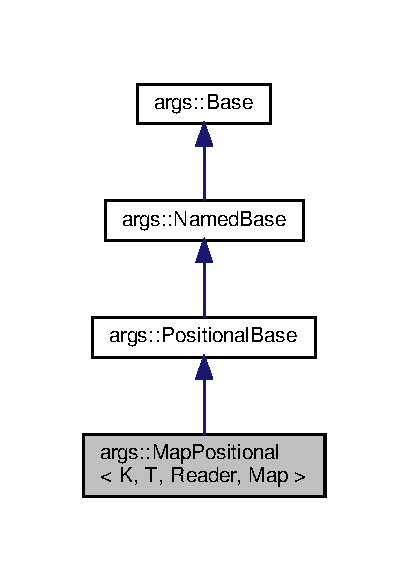
\includegraphics[width=196pt]{classargs_1_1_map_positional__inherit__graph}
\end{center}
\end{figure}


Collaboration diagram for args\+:\+:Map\+Positional$<$ K, T, Reader, Map $>$\+:\nopagebreak
\begin{figure}[H]
\begin{center}
\leavevmode
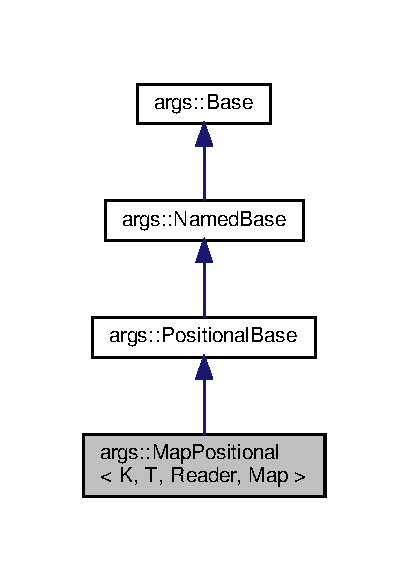
\includegraphics[width=196pt]{classargs_1_1_map_positional__coll__graph}
\end{center}
\end{figure}
\subsection*{Public Member Functions}
\begin{DoxyCompactItemize}
\item 
\hyperlink{classargs_1_1_map_positional_a5ffc44de32246532effe895152e066bc}{Map\+Positional} (\hyperlink{classargs_1_1_group}{Group} \&group\+\_\+, const std\+::string \&name\+\_\+, const std\+::string \&help\+\_\+, const Map$<$ \hyperlink{cgal__test_8cpp_a891e241aa245ae63618f03737efba309}{K}, T $>$ \&map\+\_\+, const T \&default\+Value\+\_\+=T())
\item 
virtual \hyperlink{classargs_1_1_map_positional_a6ac22277778b53bfec47cc6e244ef29c}{$\sim$\+Map\+Positional} ()
\item 
virtual void \hyperlink{classargs_1_1_map_positional_a8ac67b0ee5008bd6c9a39974c2a40ee4}{Parse\+Value} (const std\+::string \&value\+\_\+) override
\item 
T \& \hyperlink{classargs_1_1_map_positional_a46e4f230ddbca26b7eb849fd3d87510d}{Get} () noexcept
\end{DoxyCompactItemize}
\subsection*{Additional Inherited Members}


\subsection{Detailed Description}
\subsubsection*{template$<$typename K, typename T, typename Reader = Value\+Reader, template$<$ typename... $>$ class Map = std\+::unordered\+\_\+map$>$\newline
class args\+::\+Map\+Positional$<$ K, T, Reader, Map $>$}

A positional argument mapping class


\begin{DoxyTemplParams}{Template Parameters}
{\em K} & the type to extract the argument as \\
\hline
{\em T} & the type to store the result as \\
\hline
{\em Reader} & The functor type used to read the argument, taking the name, value, and destination reference with operator(), and returning a bool (if A\+R\+G\+S\+\_\+\+N\+O\+E\+X\+C\+E\+PT is defined) \\
\hline
{\em Map} & The Map type. Should operate like std\+::map or std\+::unordered\+\_\+map \\
\hline
\end{DoxyTemplParams}


\subsection{Constructor \& Destructor Documentation}
\mbox{\Hypertarget{classargs_1_1_map_positional_a5ffc44de32246532effe895152e066bc}\label{classargs_1_1_map_positional_a5ffc44de32246532effe895152e066bc}} 
\index{args\+::\+Map\+Positional@{args\+::\+Map\+Positional}!Map\+Positional@{Map\+Positional}}
\index{Map\+Positional@{Map\+Positional}!args\+::\+Map\+Positional@{args\+::\+Map\+Positional}}
\subsubsection{\texorpdfstring{Map\+Positional()}{MapPositional()}}
{\footnotesize\ttfamily template$<$typename K , typename T , typename Reader  = Value\+Reader, template$<$ typename... $>$ class Map = std\+::unordered\+\_\+map$>$ \\
\hyperlink{classargs_1_1_map_positional}{args\+::\+Map\+Positional}$<$ \hyperlink{cgal__test_8cpp_a891e241aa245ae63618f03737efba309}{K}, T, Reader, Map $>$\+::\hyperlink{classargs_1_1_map_positional}{Map\+Positional} (\begin{DoxyParamCaption}\item[{\hyperlink{classargs_1_1_group}{Group} \&}]{group\+\_\+,  }\item[{const std\+::string \&}]{name\+\_\+,  }\item[{const std\+::string \&}]{help\+\_\+,  }\item[{const Map$<$ \hyperlink{cgal__test_8cpp_a891e241aa245ae63618f03737efba309}{K}, T $>$ \&}]{map\+\_\+,  }\item[{const T \&}]{default\+Value\+\_\+ = {\ttfamily T()} }\end{DoxyParamCaption})\hspace{0.3cm}{\ttfamily [inline]}}

\mbox{\Hypertarget{classargs_1_1_map_positional_a6ac22277778b53bfec47cc6e244ef29c}\label{classargs_1_1_map_positional_a6ac22277778b53bfec47cc6e244ef29c}} 
\index{args\+::\+Map\+Positional@{args\+::\+Map\+Positional}!````~Map\+Positional@{$\sim$\+Map\+Positional}}
\index{````~Map\+Positional@{$\sim$\+Map\+Positional}!args\+::\+Map\+Positional@{args\+::\+Map\+Positional}}
\subsubsection{\texorpdfstring{$\sim$\+Map\+Positional()}{~MapPositional()}}
{\footnotesize\ttfamily template$<$typename K , typename T , typename Reader  = Value\+Reader, template$<$ typename... $>$ class Map = std\+::unordered\+\_\+map$>$ \\
virtual \hyperlink{classargs_1_1_map_positional}{args\+::\+Map\+Positional}$<$ \hyperlink{cgal__test_8cpp_a891e241aa245ae63618f03737efba309}{K}, T, Reader, Map $>$\+::$\sim$\hyperlink{classargs_1_1_map_positional}{Map\+Positional} (\begin{DoxyParamCaption}{ }\end{DoxyParamCaption})\hspace{0.3cm}{\ttfamily [inline]}, {\ttfamily [virtual]}}



\subsection{Member Function Documentation}
\mbox{\Hypertarget{classargs_1_1_map_positional_a46e4f230ddbca26b7eb849fd3d87510d}\label{classargs_1_1_map_positional_a46e4f230ddbca26b7eb849fd3d87510d}} 
\index{args\+::\+Map\+Positional@{args\+::\+Map\+Positional}!Get@{Get}}
\index{Get@{Get}!args\+::\+Map\+Positional@{args\+::\+Map\+Positional}}
\subsubsection{\texorpdfstring{Get()}{Get()}}
{\footnotesize\ttfamily template$<$typename K , typename T , typename Reader  = Value\+Reader, template$<$ typename... $>$ class Map = std\+::unordered\+\_\+map$>$ \\
T\& \hyperlink{classargs_1_1_map_positional}{args\+::\+Map\+Positional}$<$ \hyperlink{cgal__test_8cpp_a891e241aa245ae63618f03737efba309}{K}, T, Reader, Map $>$\+::Get (\begin{DoxyParamCaption}{ }\end{DoxyParamCaption})\hspace{0.3cm}{\ttfamily [inline]}, {\ttfamily [noexcept]}}

Get the value \mbox{\Hypertarget{classargs_1_1_map_positional_a8ac67b0ee5008bd6c9a39974c2a40ee4}\label{classargs_1_1_map_positional_a8ac67b0ee5008bd6c9a39974c2a40ee4}} 
\index{args\+::\+Map\+Positional@{args\+::\+Map\+Positional}!Parse\+Value@{Parse\+Value}}
\index{Parse\+Value@{Parse\+Value}!args\+::\+Map\+Positional@{args\+::\+Map\+Positional}}
\subsubsection{\texorpdfstring{Parse\+Value()}{ParseValue()}}
{\footnotesize\ttfamily template$<$typename K , typename T , typename Reader  = Value\+Reader, template$<$ typename... $>$ class Map = std\+::unordered\+\_\+map$>$ \\
virtual void \hyperlink{classargs_1_1_map_positional}{args\+::\+Map\+Positional}$<$ \hyperlink{cgal__test_8cpp_a891e241aa245ae63618f03737efba309}{K}, T, Reader, Map $>$\+::Parse\+Value (\begin{DoxyParamCaption}\item[{const std\+::string \&}]{value\+\_\+ }\end{DoxyParamCaption})\hspace{0.3cm}{\ttfamily [inline]}, {\ttfamily [override]}, {\ttfamily [virtual]}}



Implements \hyperlink{classargs_1_1_positional_base_a10b6b91155f56bc28ca25fa87c6f0985}{args\+::\+Positional\+Base}.



The documentation for this class was generated from the following file\+:\begin{DoxyCompactItemize}
\item 
/home/cappelletto/github/self/landing\+\_\+area\+\_\+detector/external/\hyperlink{args_8hxx}{args.\+hxx}\end{DoxyCompactItemize}

\hypertarget{classargs_1_1_map_positional_list}{}\section{args\+:\+:Map\+Positional\+List$<$ K, T, List, Reader, Map $>$ Class Template Reference}
\label{classargs_1_1_map_positional_list}\index{args\+::\+Map\+Positional\+List$<$ K, T, List, Reader, Map $>$@{args\+::\+Map\+Positional\+List$<$ K, T, List, Reader, Map $>$}}


{\ttfamily \#include $<$args.\+hxx$>$}



Inheritance diagram for args\+:\+:Map\+Positional\+List$<$ K, T, List, Reader, Map $>$\+:\nopagebreak
\begin{figure}[H]
\begin{center}
\leavevmode
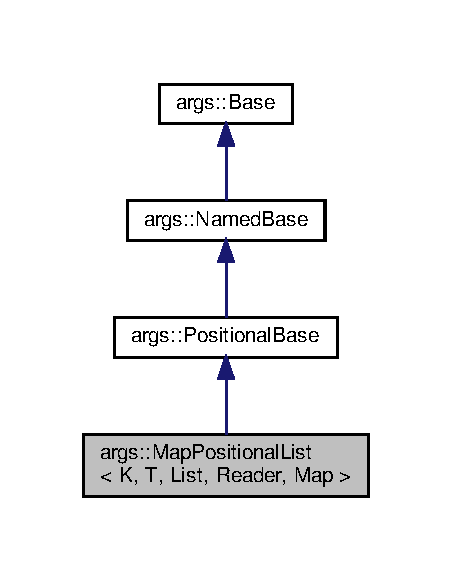
\includegraphics[width=217pt]{classargs_1_1_map_positional_list__inherit__graph}
\end{center}
\end{figure}


Collaboration diagram for args\+:\+:Map\+Positional\+List$<$ K, T, List, Reader, Map $>$\+:\nopagebreak
\begin{figure}[H]
\begin{center}
\leavevmode
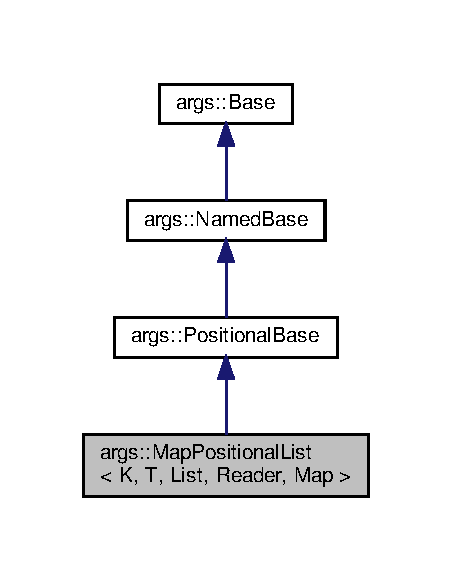
\includegraphics[width=217pt]{classargs_1_1_map_positional_list__coll__graph}
\end{center}
\end{figure}
\subsection*{Public Types}
\begin{DoxyCompactItemize}
\item 
typedef T \hyperlink{classargs_1_1_map_positional_list_aab45440653898824437c3ab443bb4bd7}{value\+\_\+type}
\item 
typedef Container\+::allocator\+\_\+type \hyperlink{classargs_1_1_map_positional_list_aa961fcc8eee61814bd1fb2b75f0235c1}{allocator\+\_\+type}
\item 
typedef Container\+::pointer \hyperlink{classargs_1_1_map_positional_list_ac005fb0e2fa99bc6e6b39103cb605d17}{pointer}
\item 
typedef Container\+::const\+\_\+pointer \hyperlink{classargs_1_1_map_positional_list_aa4ce0fca25572ffad42a9b2b9c86c691}{const\+\_\+pointer}
\item 
typedef T \& \hyperlink{classargs_1_1_map_positional_list_acabe5d01f2f750a05a8a6549a61a8120}{reference}
\item 
typedef const T \& \hyperlink{classargs_1_1_map_positional_list_a49c2fa40c50f8d1c4f3ef6023761972d}{const\+\_\+reference}
\item 
typedef Container\+::size\+\_\+type \hyperlink{classargs_1_1_map_positional_list_a217bf984e4c1108f5e4785cef1de1a95}{size\+\_\+type}
\item 
typedef Container\+::difference\+\_\+type \hyperlink{classargs_1_1_map_positional_list_a60aba0aee19ccedfcfd02074339d0e1c}{difference\+\_\+type}
\item 
typedef Container\+::iterator \hyperlink{classargs_1_1_map_positional_list_a4e3fbeb6f894505ce48d35fe76dc157a}{iterator}
\item 
typedef Container\+::const\+\_\+iterator \hyperlink{classargs_1_1_map_positional_list_a0700556b0a067e095ee22edbb18206fc}{const\+\_\+iterator}
\item 
typedef std\+::reverse\+\_\+iterator$<$ \hyperlink{classargs_1_1_map_positional_list_a4e3fbeb6f894505ce48d35fe76dc157a}{iterator} $>$ \hyperlink{classargs_1_1_map_positional_list_ad12f9031955b2dc9a3d20304a908bcea}{reverse\+\_\+iterator}
\item 
typedef std\+::reverse\+\_\+iterator$<$ \hyperlink{classargs_1_1_map_positional_list_a0700556b0a067e095ee22edbb18206fc}{const\+\_\+iterator} $>$ \hyperlink{classargs_1_1_map_positional_list_a89cd057f52f097ccd3d3072f62eacd47}{const\+\_\+reverse\+\_\+iterator}
\end{DoxyCompactItemize}
\subsection*{Public Member Functions}
\begin{DoxyCompactItemize}
\item 
\hyperlink{classargs_1_1_map_positional_list_ab8dc23a5947d8f10d0e71d907248f52f}{Map\+Positional\+List} (\hyperlink{classargs_1_1_group}{Group} \&group\+\_\+, const std\+::string \&name\+\_\+, const std\+::string \&help\+\_\+, const Map$<$ \hyperlink{cgal__test_8cpp_a891e241aa245ae63618f03737efba309}{K}, T $>$ \&map\+\_\+, const Container \&default\+Values\+\_\+=Container())
\item 
virtual \hyperlink{classargs_1_1_map_positional_list_acd2d9a2a9dafb35ff7d85b2aebe4d94e}{$\sim$\+Map\+Positional\+List} ()
\item 
virtual void \hyperlink{classargs_1_1_map_positional_list_ac2d042c42bc771954f340dc0a3b582c7}{Parse\+Value} (const std\+::string \&value\+\_\+) override
\item 
Container \& \hyperlink{classargs_1_1_map_positional_list_ad34d106fb81d46943392c74fb987fd27}{Get} () noexcept
\item 
virtual std\+::string \hyperlink{classargs_1_1_map_positional_list_a06d9cd19fea86e0027f2ab4a491f19bb}{Name} () const override
\item 
virtual void \hyperlink{classargs_1_1_map_positional_list_a69eefecdabf07a4fac7006acb2b144d3}{Reset} () noexcept override
\item 
\hyperlink{classargs_1_1_map_positional_list_a4e3fbeb6f894505ce48d35fe76dc157a}{iterator} \hyperlink{classargs_1_1_map_positional_list_a5ec966fa9cf2064c32026b817e1a8f25}{begin} () noexcept
\item 
\hyperlink{classargs_1_1_map_positional_list_a0700556b0a067e095ee22edbb18206fc}{const\+\_\+iterator} \hyperlink{classargs_1_1_map_positional_list_a40aecf3ee765506dbf54628d6ba999a5}{begin} () const noexcept
\item 
\hyperlink{classargs_1_1_map_positional_list_a0700556b0a067e095ee22edbb18206fc}{const\+\_\+iterator} \hyperlink{classargs_1_1_map_positional_list_a5d4eda96b1f2ae63fd36b6f3a3ab80a7}{cbegin} () const noexcept
\item 
\hyperlink{classargs_1_1_map_positional_list_a4e3fbeb6f894505ce48d35fe76dc157a}{iterator} \hyperlink{classargs_1_1_map_positional_list_a3605bc6cf2e3b6d263f62938dc397148}{end} () noexcept
\item 
\hyperlink{classargs_1_1_map_positional_list_a0700556b0a067e095ee22edbb18206fc}{const\+\_\+iterator} \hyperlink{classargs_1_1_map_positional_list_a1bbe7a376ba441f6525b73e1ed00d457}{end} () const noexcept
\item 
\hyperlink{classargs_1_1_map_positional_list_a0700556b0a067e095ee22edbb18206fc}{const\+\_\+iterator} \hyperlink{classargs_1_1_map_positional_list_a2e84a5f143ad24ad1967c3f7b788dff0}{cend} () const noexcept
\end{DoxyCompactItemize}
\subsection*{Additional Inherited Members}


\subsection{Detailed Description}
\subsubsection*{template$<$typename K, typename T, template$<$ typename... $>$ class List = std\+::vector, typename Reader = Value\+Reader, template$<$ typename... $>$ class Map = std\+::unordered\+\_\+map$>$\newline
class args\+::\+Map\+Positional\+List$<$ K, T, List, Reader, Map $>$}

A positional argument mapping list class


\begin{DoxyTemplParams}{Template Parameters}
{\em K} & the type to extract the argument as \\
\hline
{\em T} & the type to store the result as \\
\hline
{\em List} & the list type that houses the values \\
\hline
{\em Reader} & The functor type used to read the argument, taking the name, value, and destination reference with operator(), and returning a bool (if A\+R\+G\+S\+\_\+\+N\+O\+E\+X\+C\+E\+PT is defined) \\
\hline
{\em Map} & The Map type. Should operate like std\+::map or std\+::unordered\+\_\+map \\
\hline
\end{DoxyTemplParams}


\subsection{Member Typedef Documentation}
\mbox{\Hypertarget{classargs_1_1_map_positional_list_aa961fcc8eee61814bd1fb2b75f0235c1}\label{classargs_1_1_map_positional_list_aa961fcc8eee61814bd1fb2b75f0235c1}} 
\index{args\+::\+Map\+Positional\+List@{args\+::\+Map\+Positional\+List}!allocator\+\_\+type@{allocator\+\_\+type}}
\index{allocator\+\_\+type@{allocator\+\_\+type}!args\+::\+Map\+Positional\+List@{args\+::\+Map\+Positional\+List}}
\subsubsection{\texorpdfstring{allocator\+\_\+type}{allocator\_type}}
{\footnotesize\ttfamily template$<$typename K , typename T , template$<$ typename... $>$ class List = std\+::vector, typename Reader  = Value\+Reader, template$<$ typename... $>$ class Map = std\+::unordered\+\_\+map$>$ \\
typedef Container\+::allocator\+\_\+type \hyperlink{classargs_1_1_map_positional_list}{args\+::\+Map\+Positional\+List}$<$ \hyperlink{cgal__test_8cpp_a891e241aa245ae63618f03737efba309}{K}, T, List, Reader, Map $>$\+::\hyperlink{classargs_1_1_map_positional_list_aa961fcc8eee61814bd1fb2b75f0235c1}{allocator\+\_\+type}}

\mbox{\Hypertarget{classargs_1_1_map_positional_list_a0700556b0a067e095ee22edbb18206fc}\label{classargs_1_1_map_positional_list_a0700556b0a067e095ee22edbb18206fc}} 
\index{args\+::\+Map\+Positional\+List@{args\+::\+Map\+Positional\+List}!const\+\_\+iterator@{const\+\_\+iterator}}
\index{const\+\_\+iterator@{const\+\_\+iterator}!args\+::\+Map\+Positional\+List@{args\+::\+Map\+Positional\+List}}
\subsubsection{\texorpdfstring{const\+\_\+iterator}{const\_iterator}}
{\footnotesize\ttfamily template$<$typename K , typename T , template$<$ typename... $>$ class List = std\+::vector, typename Reader  = Value\+Reader, template$<$ typename... $>$ class Map = std\+::unordered\+\_\+map$>$ \\
typedef Container\+::const\+\_\+iterator \hyperlink{classargs_1_1_map_positional_list}{args\+::\+Map\+Positional\+List}$<$ \hyperlink{cgal__test_8cpp_a891e241aa245ae63618f03737efba309}{K}, T, List, Reader, Map $>$\+::\hyperlink{classargs_1_1_map_positional_list_a0700556b0a067e095ee22edbb18206fc}{const\+\_\+iterator}}

\mbox{\Hypertarget{classargs_1_1_map_positional_list_aa4ce0fca25572ffad42a9b2b9c86c691}\label{classargs_1_1_map_positional_list_aa4ce0fca25572ffad42a9b2b9c86c691}} 
\index{args\+::\+Map\+Positional\+List@{args\+::\+Map\+Positional\+List}!const\+\_\+pointer@{const\+\_\+pointer}}
\index{const\+\_\+pointer@{const\+\_\+pointer}!args\+::\+Map\+Positional\+List@{args\+::\+Map\+Positional\+List}}
\subsubsection{\texorpdfstring{const\+\_\+pointer}{const\_pointer}}
{\footnotesize\ttfamily template$<$typename K , typename T , template$<$ typename... $>$ class List = std\+::vector, typename Reader  = Value\+Reader, template$<$ typename... $>$ class Map = std\+::unordered\+\_\+map$>$ \\
typedef Container\+::const\+\_\+pointer \hyperlink{classargs_1_1_map_positional_list}{args\+::\+Map\+Positional\+List}$<$ \hyperlink{cgal__test_8cpp_a891e241aa245ae63618f03737efba309}{K}, T, List, Reader, Map $>$\+::\hyperlink{classargs_1_1_map_positional_list_aa4ce0fca25572ffad42a9b2b9c86c691}{const\+\_\+pointer}}

\mbox{\Hypertarget{classargs_1_1_map_positional_list_a49c2fa40c50f8d1c4f3ef6023761972d}\label{classargs_1_1_map_positional_list_a49c2fa40c50f8d1c4f3ef6023761972d}} 
\index{args\+::\+Map\+Positional\+List@{args\+::\+Map\+Positional\+List}!const\+\_\+reference@{const\+\_\+reference}}
\index{const\+\_\+reference@{const\+\_\+reference}!args\+::\+Map\+Positional\+List@{args\+::\+Map\+Positional\+List}}
\subsubsection{\texorpdfstring{const\+\_\+reference}{const\_reference}}
{\footnotesize\ttfamily template$<$typename K , typename T , template$<$ typename... $>$ class List = std\+::vector, typename Reader  = Value\+Reader, template$<$ typename... $>$ class Map = std\+::unordered\+\_\+map$>$ \\
typedef const T\& \hyperlink{classargs_1_1_map_positional_list}{args\+::\+Map\+Positional\+List}$<$ \hyperlink{cgal__test_8cpp_a891e241aa245ae63618f03737efba309}{K}, T, List, Reader, Map $>$\+::\hyperlink{classargs_1_1_map_positional_list_a49c2fa40c50f8d1c4f3ef6023761972d}{const\+\_\+reference}}

\mbox{\Hypertarget{classargs_1_1_map_positional_list_a89cd057f52f097ccd3d3072f62eacd47}\label{classargs_1_1_map_positional_list_a89cd057f52f097ccd3d3072f62eacd47}} 
\index{args\+::\+Map\+Positional\+List@{args\+::\+Map\+Positional\+List}!const\+\_\+reverse\+\_\+iterator@{const\+\_\+reverse\+\_\+iterator}}
\index{const\+\_\+reverse\+\_\+iterator@{const\+\_\+reverse\+\_\+iterator}!args\+::\+Map\+Positional\+List@{args\+::\+Map\+Positional\+List}}
\subsubsection{\texorpdfstring{const\+\_\+reverse\+\_\+iterator}{const\_reverse\_iterator}}
{\footnotesize\ttfamily template$<$typename K , typename T , template$<$ typename... $>$ class List = std\+::vector, typename Reader  = Value\+Reader, template$<$ typename... $>$ class Map = std\+::unordered\+\_\+map$>$ \\
typedef std\+::reverse\+\_\+iterator$<$\hyperlink{classargs_1_1_map_positional_list_a0700556b0a067e095ee22edbb18206fc}{const\+\_\+iterator}$>$ \hyperlink{classargs_1_1_map_positional_list}{args\+::\+Map\+Positional\+List}$<$ \hyperlink{cgal__test_8cpp_a891e241aa245ae63618f03737efba309}{K}, T, List, Reader, Map $>$\+::\hyperlink{classargs_1_1_map_positional_list_a89cd057f52f097ccd3d3072f62eacd47}{const\+\_\+reverse\+\_\+iterator}}

\mbox{\Hypertarget{classargs_1_1_map_positional_list_a60aba0aee19ccedfcfd02074339d0e1c}\label{classargs_1_1_map_positional_list_a60aba0aee19ccedfcfd02074339d0e1c}} 
\index{args\+::\+Map\+Positional\+List@{args\+::\+Map\+Positional\+List}!difference\+\_\+type@{difference\+\_\+type}}
\index{difference\+\_\+type@{difference\+\_\+type}!args\+::\+Map\+Positional\+List@{args\+::\+Map\+Positional\+List}}
\subsubsection{\texorpdfstring{difference\+\_\+type}{difference\_type}}
{\footnotesize\ttfamily template$<$typename K , typename T , template$<$ typename... $>$ class List = std\+::vector, typename Reader  = Value\+Reader, template$<$ typename... $>$ class Map = std\+::unordered\+\_\+map$>$ \\
typedef Container\+::difference\+\_\+type \hyperlink{classargs_1_1_map_positional_list}{args\+::\+Map\+Positional\+List}$<$ \hyperlink{cgal__test_8cpp_a891e241aa245ae63618f03737efba309}{K}, T, List, Reader, Map $>$\+::\hyperlink{classargs_1_1_map_positional_list_a60aba0aee19ccedfcfd02074339d0e1c}{difference\+\_\+type}}

\mbox{\Hypertarget{classargs_1_1_map_positional_list_a4e3fbeb6f894505ce48d35fe76dc157a}\label{classargs_1_1_map_positional_list_a4e3fbeb6f894505ce48d35fe76dc157a}} 
\index{args\+::\+Map\+Positional\+List@{args\+::\+Map\+Positional\+List}!iterator@{iterator}}
\index{iterator@{iterator}!args\+::\+Map\+Positional\+List@{args\+::\+Map\+Positional\+List}}
\subsubsection{\texorpdfstring{iterator}{iterator}}
{\footnotesize\ttfamily template$<$typename K , typename T , template$<$ typename... $>$ class List = std\+::vector, typename Reader  = Value\+Reader, template$<$ typename... $>$ class Map = std\+::unordered\+\_\+map$>$ \\
typedef Container\+::iterator \hyperlink{classargs_1_1_map_positional_list}{args\+::\+Map\+Positional\+List}$<$ \hyperlink{cgal__test_8cpp_a891e241aa245ae63618f03737efba309}{K}, T, List, Reader, Map $>$\+::\hyperlink{classargs_1_1_map_positional_list_a4e3fbeb6f894505ce48d35fe76dc157a}{iterator}}

\mbox{\Hypertarget{classargs_1_1_map_positional_list_ac005fb0e2fa99bc6e6b39103cb605d17}\label{classargs_1_1_map_positional_list_ac005fb0e2fa99bc6e6b39103cb605d17}} 
\index{args\+::\+Map\+Positional\+List@{args\+::\+Map\+Positional\+List}!pointer@{pointer}}
\index{pointer@{pointer}!args\+::\+Map\+Positional\+List@{args\+::\+Map\+Positional\+List}}
\subsubsection{\texorpdfstring{pointer}{pointer}}
{\footnotesize\ttfamily template$<$typename K , typename T , template$<$ typename... $>$ class List = std\+::vector, typename Reader  = Value\+Reader, template$<$ typename... $>$ class Map = std\+::unordered\+\_\+map$>$ \\
typedef Container\+::pointer \hyperlink{classargs_1_1_map_positional_list}{args\+::\+Map\+Positional\+List}$<$ \hyperlink{cgal__test_8cpp_a891e241aa245ae63618f03737efba309}{K}, T, List, Reader, Map $>$\+::\hyperlink{classargs_1_1_map_positional_list_ac005fb0e2fa99bc6e6b39103cb605d17}{pointer}}

\mbox{\Hypertarget{classargs_1_1_map_positional_list_acabe5d01f2f750a05a8a6549a61a8120}\label{classargs_1_1_map_positional_list_acabe5d01f2f750a05a8a6549a61a8120}} 
\index{args\+::\+Map\+Positional\+List@{args\+::\+Map\+Positional\+List}!reference@{reference}}
\index{reference@{reference}!args\+::\+Map\+Positional\+List@{args\+::\+Map\+Positional\+List}}
\subsubsection{\texorpdfstring{reference}{reference}}
{\footnotesize\ttfamily template$<$typename K , typename T , template$<$ typename... $>$ class List = std\+::vector, typename Reader  = Value\+Reader, template$<$ typename... $>$ class Map = std\+::unordered\+\_\+map$>$ \\
typedef T\& \hyperlink{classargs_1_1_map_positional_list}{args\+::\+Map\+Positional\+List}$<$ \hyperlink{cgal__test_8cpp_a891e241aa245ae63618f03737efba309}{K}, T, List, Reader, Map $>$\+::\hyperlink{classargs_1_1_map_positional_list_acabe5d01f2f750a05a8a6549a61a8120}{reference}}

\mbox{\Hypertarget{classargs_1_1_map_positional_list_ad12f9031955b2dc9a3d20304a908bcea}\label{classargs_1_1_map_positional_list_ad12f9031955b2dc9a3d20304a908bcea}} 
\index{args\+::\+Map\+Positional\+List@{args\+::\+Map\+Positional\+List}!reverse\+\_\+iterator@{reverse\+\_\+iterator}}
\index{reverse\+\_\+iterator@{reverse\+\_\+iterator}!args\+::\+Map\+Positional\+List@{args\+::\+Map\+Positional\+List}}
\subsubsection{\texorpdfstring{reverse\+\_\+iterator}{reverse\_iterator}}
{\footnotesize\ttfamily template$<$typename K , typename T , template$<$ typename... $>$ class List = std\+::vector, typename Reader  = Value\+Reader, template$<$ typename... $>$ class Map = std\+::unordered\+\_\+map$>$ \\
typedef std\+::reverse\+\_\+iterator$<$\hyperlink{classargs_1_1_map_positional_list_a4e3fbeb6f894505ce48d35fe76dc157a}{iterator}$>$ \hyperlink{classargs_1_1_map_positional_list}{args\+::\+Map\+Positional\+List}$<$ \hyperlink{cgal__test_8cpp_a891e241aa245ae63618f03737efba309}{K}, T, List, Reader, Map $>$\+::\hyperlink{classargs_1_1_map_positional_list_ad12f9031955b2dc9a3d20304a908bcea}{reverse\+\_\+iterator}}

\mbox{\Hypertarget{classargs_1_1_map_positional_list_a217bf984e4c1108f5e4785cef1de1a95}\label{classargs_1_1_map_positional_list_a217bf984e4c1108f5e4785cef1de1a95}} 
\index{args\+::\+Map\+Positional\+List@{args\+::\+Map\+Positional\+List}!size\+\_\+type@{size\+\_\+type}}
\index{size\+\_\+type@{size\+\_\+type}!args\+::\+Map\+Positional\+List@{args\+::\+Map\+Positional\+List}}
\subsubsection{\texorpdfstring{size\+\_\+type}{size\_type}}
{\footnotesize\ttfamily template$<$typename K , typename T , template$<$ typename... $>$ class List = std\+::vector, typename Reader  = Value\+Reader, template$<$ typename... $>$ class Map = std\+::unordered\+\_\+map$>$ \\
typedef Container\+::size\+\_\+type \hyperlink{classargs_1_1_map_positional_list}{args\+::\+Map\+Positional\+List}$<$ \hyperlink{cgal__test_8cpp_a891e241aa245ae63618f03737efba309}{K}, T, List, Reader, Map $>$\+::\hyperlink{classargs_1_1_map_positional_list_a217bf984e4c1108f5e4785cef1de1a95}{size\+\_\+type}}

\mbox{\Hypertarget{classargs_1_1_map_positional_list_aab45440653898824437c3ab443bb4bd7}\label{classargs_1_1_map_positional_list_aab45440653898824437c3ab443bb4bd7}} 
\index{args\+::\+Map\+Positional\+List@{args\+::\+Map\+Positional\+List}!value\+\_\+type@{value\+\_\+type}}
\index{value\+\_\+type@{value\+\_\+type}!args\+::\+Map\+Positional\+List@{args\+::\+Map\+Positional\+List}}
\subsubsection{\texorpdfstring{value\+\_\+type}{value\_type}}
{\footnotesize\ttfamily template$<$typename K , typename T , template$<$ typename... $>$ class List = std\+::vector, typename Reader  = Value\+Reader, template$<$ typename... $>$ class Map = std\+::unordered\+\_\+map$>$ \\
typedef T \hyperlink{classargs_1_1_map_positional_list}{args\+::\+Map\+Positional\+List}$<$ \hyperlink{cgal__test_8cpp_a891e241aa245ae63618f03737efba309}{K}, T, List, Reader, Map $>$\+::\hyperlink{classargs_1_1_map_positional_list_aab45440653898824437c3ab443bb4bd7}{value\+\_\+type}}



\subsection{Constructor \& Destructor Documentation}
\mbox{\Hypertarget{classargs_1_1_map_positional_list_ab8dc23a5947d8f10d0e71d907248f52f}\label{classargs_1_1_map_positional_list_ab8dc23a5947d8f10d0e71d907248f52f}} 
\index{args\+::\+Map\+Positional\+List@{args\+::\+Map\+Positional\+List}!Map\+Positional\+List@{Map\+Positional\+List}}
\index{Map\+Positional\+List@{Map\+Positional\+List}!args\+::\+Map\+Positional\+List@{args\+::\+Map\+Positional\+List}}
\subsubsection{\texorpdfstring{Map\+Positional\+List()}{MapPositionalList()}}
{\footnotesize\ttfamily template$<$typename K , typename T , template$<$ typename... $>$ class List = std\+::vector, typename Reader  = Value\+Reader, template$<$ typename... $>$ class Map = std\+::unordered\+\_\+map$>$ \\
\hyperlink{classargs_1_1_map_positional_list}{args\+::\+Map\+Positional\+List}$<$ \hyperlink{cgal__test_8cpp_a891e241aa245ae63618f03737efba309}{K}, T, List, Reader, Map $>$\+::\hyperlink{classargs_1_1_map_positional_list}{Map\+Positional\+List} (\begin{DoxyParamCaption}\item[{\hyperlink{classargs_1_1_group}{Group} \&}]{group\+\_\+,  }\item[{const std\+::string \&}]{name\+\_\+,  }\item[{const std\+::string \&}]{help\+\_\+,  }\item[{const Map$<$ \hyperlink{cgal__test_8cpp_a891e241aa245ae63618f03737efba309}{K}, T $>$ \&}]{map\+\_\+,  }\item[{const Container \&}]{default\+Values\+\_\+ = {\ttfamily Container()} }\end{DoxyParamCaption})\hspace{0.3cm}{\ttfamily [inline]}}

\mbox{\Hypertarget{classargs_1_1_map_positional_list_acd2d9a2a9dafb35ff7d85b2aebe4d94e}\label{classargs_1_1_map_positional_list_acd2d9a2a9dafb35ff7d85b2aebe4d94e}} 
\index{args\+::\+Map\+Positional\+List@{args\+::\+Map\+Positional\+List}!````~Map\+Positional\+List@{$\sim$\+Map\+Positional\+List}}
\index{````~Map\+Positional\+List@{$\sim$\+Map\+Positional\+List}!args\+::\+Map\+Positional\+List@{args\+::\+Map\+Positional\+List}}
\subsubsection{\texorpdfstring{$\sim$\+Map\+Positional\+List()}{~MapPositionalList()}}
{\footnotesize\ttfamily template$<$typename K , typename T , template$<$ typename... $>$ class List = std\+::vector, typename Reader  = Value\+Reader, template$<$ typename... $>$ class Map = std\+::unordered\+\_\+map$>$ \\
virtual \hyperlink{classargs_1_1_map_positional_list}{args\+::\+Map\+Positional\+List}$<$ \hyperlink{cgal__test_8cpp_a891e241aa245ae63618f03737efba309}{K}, T, List, Reader, Map $>$\+::$\sim$\hyperlink{classargs_1_1_map_positional_list}{Map\+Positional\+List} (\begin{DoxyParamCaption}{ }\end{DoxyParamCaption})\hspace{0.3cm}{\ttfamily [inline]}, {\ttfamily [virtual]}}



\subsection{Member Function Documentation}
\mbox{\Hypertarget{classargs_1_1_map_positional_list_a5ec966fa9cf2064c32026b817e1a8f25}\label{classargs_1_1_map_positional_list_a5ec966fa9cf2064c32026b817e1a8f25}} 
\index{args\+::\+Map\+Positional\+List@{args\+::\+Map\+Positional\+List}!begin@{begin}}
\index{begin@{begin}!args\+::\+Map\+Positional\+List@{args\+::\+Map\+Positional\+List}}
\subsubsection{\texorpdfstring{begin()}{begin()}\hspace{0.1cm}{\footnotesize\ttfamily [1/2]}}
{\footnotesize\ttfamily template$<$typename K , typename T , template$<$ typename... $>$ class List = std\+::vector, typename Reader  = Value\+Reader, template$<$ typename... $>$ class Map = std\+::unordered\+\_\+map$>$ \\
\hyperlink{classargs_1_1_map_positional_list_a4e3fbeb6f894505ce48d35fe76dc157a}{iterator} \hyperlink{classargs_1_1_map_positional_list}{args\+::\+Map\+Positional\+List}$<$ \hyperlink{cgal__test_8cpp_a891e241aa245ae63618f03737efba309}{K}, T, List, Reader, Map $>$\+::begin (\begin{DoxyParamCaption}{ }\end{DoxyParamCaption})\hspace{0.3cm}{\ttfamily [inline]}, {\ttfamily [noexcept]}}

\mbox{\Hypertarget{classargs_1_1_map_positional_list_a40aecf3ee765506dbf54628d6ba999a5}\label{classargs_1_1_map_positional_list_a40aecf3ee765506dbf54628d6ba999a5}} 
\index{args\+::\+Map\+Positional\+List@{args\+::\+Map\+Positional\+List}!begin@{begin}}
\index{begin@{begin}!args\+::\+Map\+Positional\+List@{args\+::\+Map\+Positional\+List}}
\subsubsection{\texorpdfstring{begin()}{begin()}\hspace{0.1cm}{\footnotesize\ttfamily [2/2]}}
{\footnotesize\ttfamily template$<$typename K , typename T , template$<$ typename... $>$ class List = std\+::vector, typename Reader  = Value\+Reader, template$<$ typename... $>$ class Map = std\+::unordered\+\_\+map$>$ \\
\hyperlink{classargs_1_1_map_positional_list_a0700556b0a067e095ee22edbb18206fc}{const\+\_\+iterator} \hyperlink{classargs_1_1_map_positional_list}{args\+::\+Map\+Positional\+List}$<$ \hyperlink{cgal__test_8cpp_a891e241aa245ae63618f03737efba309}{K}, T, List, Reader, Map $>$\+::begin (\begin{DoxyParamCaption}{ }\end{DoxyParamCaption}) const\hspace{0.3cm}{\ttfamily [inline]}, {\ttfamily [noexcept]}}

\mbox{\Hypertarget{classargs_1_1_map_positional_list_a5d4eda96b1f2ae63fd36b6f3a3ab80a7}\label{classargs_1_1_map_positional_list_a5d4eda96b1f2ae63fd36b6f3a3ab80a7}} 
\index{args\+::\+Map\+Positional\+List@{args\+::\+Map\+Positional\+List}!cbegin@{cbegin}}
\index{cbegin@{cbegin}!args\+::\+Map\+Positional\+List@{args\+::\+Map\+Positional\+List}}
\subsubsection{\texorpdfstring{cbegin()}{cbegin()}}
{\footnotesize\ttfamily template$<$typename K , typename T , template$<$ typename... $>$ class List = std\+::vector, typename Reader  = Value\+Reader, template$<$ typename... $>$ class Map = std\+::unordered\+\_\+map$>$ \\
\hyperlink{classargs_1_1_map_positional_list_a0700556b0a067e095ee22edbb18206fc}{const\+\_\+iterator} \hyperlink{classargs_1_1_map_positional_list}{args\+::\+Map\+Positional\+List}$<$ \hyperlink{cgal__test_8cpp_a891e241aa245ae63618f03737efba309}{K}, T, List, Reader, Map $>$\+::cbegin (\begin{DoxyParamCaption}{ }\end{DoxyParamCaption}) const\hspace{0.3cm}{\ttfamily [inline]}, {\ttfamily [noexcept]}}

\mbox{\Hypertarget{classargs_1_1_map_positional_list_a2e84a5f143ad24ad1967c3f7b788dff0}\label{classargs_1_1_map_positional_list_a2e84a5f143ad24ad1967c3f7b788dff0}} 
\index{args\+::\+Map\+Positional\+List@{args\+::\+Map\+Positional\+List}!cend@{cend}}
\index{cend@{cend}!args\+::\+Map\+Positional\+List@{args\+::\+Map\+Positional\+List}}
\subsubsection{\texorpdfstring{cend()}{cend()}}
{\footnotesize\ttfamily template$<$typename K , typename T , template$<$ typename... $>$ class List = std\+::vector, typename Reader  = Value\+Reader, template$<$ typename... $>$ class Map = std\+::unordered\+\_\+map$>$ \\
\hyperlink{classargs_1_1_map_positional_list_a0700556b0a067e095ee22edbb18206fc}{const\+\_\+iterator} \hyperlink{classargs_1_1_map_positional_list}{args\+::\+Map\+Positional\+List}$<$ \hyperlink{cgal__test_8cpp_a891e241aa245ae63618f03737efba309}{K}, T, List, Reader, Map $>$\+::cend (\begin{DoxyParamCaption}{ }\end{DoxyParamCaption}) const\hspace{0.3cm}{\ttfamily [inline]}, {\ttfamily [noexcept]}}

\mbox{\Hypertarget{classargs_1_1_map_positional_list_a3605bc6cf2e3b6d263f62938dc397148}\label{classargs_1_1_map_positional_list_a3605bc6cf2e3b6d263f62938dc397148}} 
\index{args\+::\+Map\+Positional\+List@{args\+::\+Map\+Positional\+List}!end@{end}}
\index{end@{end}!args\+::\+Map\+Positional\+List@{args\+::\+Map\+Positional\+List}}
\subsubsection{\texorpdfstring{end()}{end()}\hspace{0.1cm}{\footnotesize\ttfamily [1/2]}}
{\footnotesize\ttfamily template$<$typename K , typename T , template$<$ typename... $>$ class List = std\+::vector, typename Reader  = Value\+Reader, template$<$ typename... $>$ class Map = std\+::unordered\+\_\+map$>$ \\
\hyperlink{classargs_1_1_map_positional_list_a4e3fbeb6f894505ce48d35fe76dc157a}{iterator} \hyperlink{classargs_1_1_map_positional_list}{args\+::\+Map\+Positional\+List}$<$ \hyperlink{cgal__test_8cpp_a891e241aa245ae63618f03737efba309}{K}, T, List, Reader, Map $>$\+::end (\begin{DoxyParamCaption}{ }\end{DoxyParamCaption})\hspace{0.3cm}{\ttfamily [inline]}, {\ttfamily [noexcept]}}

\mbox{\Hypertarget{classargs_1_1_map_positional_list_a1bbe7a376ba441f6525b73e1ed00d457}\label{classargs_1_1_map_positional_list_a1bbe7a376ba441f6525b73e1ed00d457}} 
\index{args\+::\+Map\+Positional\+List@{args\+::\+Map\+Positional\+List}!end@{end}}
\index{end@{end}!args\+::\+Map\+Positional\+List@{args\+::\+Map\+Positional\+List}}
\subsubsection{\texorpdfstring{end()}{end()}\hspace{0.1cm}{\footnotesize\ttfamily [2/2]}}
{\footnotesize\ttfamily template$<$typename K , typename T , template$<$ typename... $>$ class List = std\+::vector, typename Reader  = Value\+Reader, template$<$ typename... $>$ class Map = std\+::unordered\+\_\+map$>$ \\
\hyperlink{classargs_1_1_map_positional_list_a0700556b0a067e095ee22edbb18206fc}{const\+\_\+iterator} \hyperlink{classargs_1_1_map_positional_list}{args\+::\+Map\+Positional\+List}$<$ \hyperlink{cgal__test_8cpp_a891e241aa245ae63618f03737efba309}{K}, T, List, Reader, Map $>$\+::end (\begin{DoxyParamCaption}{ }\end{DoxyParamCaption}) const\hspace{0.3cm}{\ttfamily [inline]}, {\ttfamily [noexcept]}}

\mbox{\Hypertarget{classargs_1_1_map_positional_list_ad34d106fb81d46943392c74fb987fd27}\label{classargs_1_1_map_positional_list_ad34d106fb81d46943392c74fb987fd27}} 
\index{args\+::\+Map\+Positional\+List@{args\+::\+Map\+Positional\+List}!Get@{Get}}
\index{Get@{Get}!args\+::\+Map\+Positional\+List@{args\+::\+Map\+Positional\+List}}
\subsubsection{\texorpdfstring{Get()}{Get()}}
{\footnotesize\ttfamily template$<$typename K , typename T , template$<$ typename... $>$ class List = std\+::vector, typename Reader  = Value\+Reader, template$<$ typename... $>$ class Map = std\+::unordered\+\_\+map$>$ \\
Container\& \hyperlink{classargs_1_1_map_positional_list}{args\+::\+Map\+Positional\+List}$<$ \hyperlink{cgal__test_8cpp_a891e241aa245ae63618f03737efba309}{K}, T, List, Reader, Map $>$\+::Get (\begin{DoxyParamCaption}{ }\end{DoxyParamCaption})\hspace{0.3cm}{\ttfamily [inline]}, {\ttfamily [noexcept]}}

Get the value \mbox{\Hypertarget{classargs_1_1_map_positional_list_a06d9cd19fea86e0027f2ab4a491f19bb}\label{classargs_1_1_map_positional_list_a06d9cd19fea86e0027f2ab4a491f19bb}} 
\index{args\+::\+Map\+Positional\+List@{args\+::\+Map\+Positional\+List}!Name@{Name}}
\index{Name@{Name}!args\+::\+Map\+Positional\+List@{args\+::\+Map\+Positional\+List}}
\subsubsection{\texorpdfstring{Name()}{Name()}}
{\footnotesize\ttfamily template$<$typename K , typename T , template$<$ typename... $>$ class List = std\+::vector, typename Reader  = Value\+Reader, template$<$ typename... $>$ class Map = std\+::unordered\+\_\+map$>$ \\
virtual std\+::string \hyperlink{classargs_1_1_map_positional_list}{args\+::\+Map\+Positional\+List}$<$ \hyperlink{cgal__test_8cpp_a891e241aa245ae63618f03737efba309}{K}, T, List, Reader, Map $>$\+::Name (\begin{DoxyParamCaption}{ }\end{DoxyParamCaption}) const\hspace{0.3cm}{\ttfamily [inline]}, {\ttfamily [override]}, {\ttfamily [virtual]}}



Reimplemented from \hyperlink{classargs_1_1_named_base_a7e7bab5c0de59e717b87935b14376dfc}{args\+::\+Named\+Base}.

\mbox{\Hypertarget{classargs_1_1_map_positional_list_ac2d042c42bc771954f340dc0a3b582c7}\label{classargs_1_1_map_positional_list_ac2d042c42bc771954f340dc0a3b582c7}} 
\index{args\+::\+Map\+Positional\+List@{args\+::\+Map\+Positional\+List}!Parse\+Value@{Parse\+Value}}
\index{Parse\+Value@{Parse\+Value}!args\+::\+Map\+Positional\+List@{args\+::\+Map\+Positional\+List}}
\subsubsection{\texorpdfstring{Parse\+Value()}{ParseValue()}}
{\footnotesize\ttfamily template$<$typename K , typename T , template$<$ typename... $>$ class List = std\+::vector, typename Reader  = Value\+Reader, template$<$ typename... $>$ class Map = std\+::unordered\+\_\+map$>$ \\
virtual void \hyperlink{classargs_1_1_map_positional_list}{args\+::\+Map\+Positional\+List}$<$ \hyperlink{cgal__test_8cpp_a891e241aa245ae63618f03737efba309}{K}, T, List, Reader, Map $>$\+::Parse\+Value (\begin{DoxyParamCaption}\item[{const std\+::string \&}]{value\+\_\+ }\end{DoxyParamCaption})\hspace{0.3cm}{\ttfamily [inline]}, {\ttfamily [override]}, {\ttfamily [virtual]}}



Implements \hyperlink{classargs_1_1_positional_base_a10b6b91155f56bc28ca25fa87c6f0985}{args\+::\+Positional\+Base}.

\mbox{\Hypertarget{classargs_1_1_map_positional_list_a69eefecdabf07a4fac7006acb2b144d3}\label{classargs_1_1_map_positional_list_a69eefecdabf07a4fac7006acb2b144d3}} 
\index{args\+::\+Map\+Positional\+List@{args\+::\+Map\+Positional\+List}!Reset@{Reset}}
\index{Reset@{Reset}!args\+::\+Map\+Positional\+List@{args\+::\+Map\+Positional\+List}}
\subsubsection{\texorpdfstring{Reset()}{Reset()}}
{\footnotesize\ttfamily template$<$typename K , typename T , template$<$ typename... $>$ class List = std\+::vector, typename Reader  = Value\+Reader, template$<$ typename... $>$ class Map = std\+::unordered\+\_\+map$>$ \\
virtual void \hyperlink{classargs_1_1_map_positional_list}{args\+::\+Map\+Positional\+List}$<$ \hyperlink{cgal__test_8cpp_a891e241aa245ae63618f03737efba309}{K}, T, List, Reader, Map $>$\+::Reset (\begin{DoxyParamCaption}{ }\end{DoxyParamCaption})\hspace{0.3cm}{\ttfamily [inline]}, {\ttfamily [override]}, {\ttfamily [virtual]}, {\ttfamily [noexcept]}}



Reimplemented from \hyperlink{classargs_1_1_positional_base_a14edfb214858983cf5116c8d0fec72ea}{args\+::\+Positional\+Base}.



The documentation for this class was generated from the following file\+:\begin{DoxyCompactItemize}
\item 
/home/cappelletto/github/self/landing\+\_\+area\+\_\+detector/external/\hyperlink{args_8hxx}{args.\+hxx}\end{DoxyCompactItemize}

\hypertarget{classargs_1_1_matcher}{}\section{args\+:\+:Matcher Class Reference}
\label{classargs_1_1_matcher}\index{args\+::\+Matcher@{args\+::\+Matcher}}


{\ttfamily \#include $<$args.\+hxx$>$}

\subsection*{Public Member Functions}
\begin{DoxyCompactItemize}
\item 
{\footnotesize template$<$typename Short\+It , typename Long\+It $>$ }\\\hyperlink{classargs_1_1_matcher_a87fc200d9a51b3be654e0ec551304ec5}{Matcher} (Short\+It short\+Flags\+Start, Short\+It short\+Flags\+End, Long\+It long\+Flags\+Start, Long\+It long\+Flags\+End)
\item 
{\footnotesize template$<$typename Short , typename Long $>$ }\\\hyperlink{classargs_1_1_matcher_a62cfbb3db70f623153f8317abb5421dc}{Matcher} (Short \&\&short\+In, Long \&\&long\+In)
\item 
\hyperlink{classargs_1_1_matcher_ad70f96e5475d9020773b429e9f79cb2d}{Matcher} (std\+::initializer\+\_\+list$<$ \hyperlink{structargs_1_1_either_flag}{Either\+Flag} $>$ in)
\item 
\hyperlink{classargs_1_1_matcher_a29ef34a8f70f00dfb52c9d5d15886625}{Matcher} (\hyperlink{classargs_1_1_matcher}{Matcher} \&\&other)
\item 
\hyperlink{classargs_1_1_matcher_acb9ecd5c9f54e07e5457dcabbfb8d9cd}{$\sim$\+Matcher} ()
\item 
bool \hyperlink{classargs_1_1_matcher_ac0109d749d161b039d879e2c6b4b708c}{Match} (const char flag) const
\item 
bool \hyperlink{classargs_1_1_matcher_aa61c6a4d756752ec692c0b703035608a}{Match} (const std\+::string \&flag) const
\item 
bool \hyperlink{classargs_1_1_matcher_ad657c9f5cca2892863c71bb980ea94e2}{Match} (const \hyperlink{structargs_1_1_either_flag}{Either\+Flag} \&flag) const
\item 
std\+::vector$<$ \hyperlink{structargs_1_1_either_flag}{Either\+Flag} $>$ \hyperlink{classargs_1_1_matcher_a3b90feb46bb0d504072344e8bced8cd5}{Get\+Flag\+Strings} () const
\item 
\hyperlink{structargs_1_1_either_flag}{Either\+Flag} \hyperlink{classargs_1_1_matcher_ab3668d21d135ca54f966b935a5251836}{Get\+Long\+Or\+Any} () const
\item 
\hyperlink{structargs_1_1_either_flag}{Either\+Flag} \hyperlink{classargs_1_1_matcher_a41ff39211bfb881c95b69b9d4e1e3b00}{Get\+Short\+Or\+Any} () const
\end{DoxyCompactItemize}


\subsection{Detailed Description}
A class of \char`\"{}matchers\char`\"{}, specifying short and flags that can possibly be matched.

This is supposed to be constructed and then passed in, not used directly from user code. 

\subsection{Constructor \& Destructor Documentation}
\mbox{\Hypertarget{classargs_1_1_matcher_a87fc200d9a51b3be654e0ec551304ec5}\label{classargs_1_1_matcher_a87fc200d9a51b3be654e0ec551304ec5}} 
\index{args\+::\+Matcher@{args\+::\+Matcher}!Matcher@{Matcher}}
\index{Matcher@{Matcher}!args\+::\+Matcher@{args\+::\+Matcher}}
\subsubsection{\texorpdfstring{Matcher()}{Matcher()}\hspace{0.1cm}{\footnotesize\ttfamily [1/4]}}
{\footnotesize\ttfamily template$<$typename Short\+It , typename Long\+It $>$ \\
args\+::\+Matcher\+::\+Matcher (\begin{DoxyParamCaption}\item[{Short\+It}]{short\+Flags\+Start,  }\item[{Short\+It}]{short\+Flags\+End,  }\item[{Long\+It}]{long\+Flags\+Start,  }\item[{Long\+It}]{long\+Flags\+End }\end{DoxyParamCaption})\hspace{0.3cm}{\ttfamily [inline]}}

Specify short and long flags separately as iterators

ex\+: {\ttfamily \hyperlink{classargs_1_1_matcher}{args\+::\+Matcher}(short\+Flags.\+begin(), short\+Flags.\+end(), long\+Flags.\+begin(), long\+Flags.\+end())} \mbox{\Hypertarget{classargs_1_1_matcher_a62cfbb3db70f623153f8317abb5421dc}\label{classargs_1_1_matcher_a62cfbb3db70f623153f8317abb5421dc}} 
\index{args\+::\+Matcher@{args\+::\+Matcher}!Matcher@{Matcher}}
\index{Matcher@{Matcher}!args\+::\+Matcher@{args\+::\+Matcher}}
\subsubsection{\texorpdfstring{Matcher()}{Matcher()}\hspace{0.1cm}{\footnotesize\ttfamily [2/4]}}
{\footnotesize\ttfamily template$<$typename Short , typename Long $>$ \\
args\+::\+Matcher\+::\+Matcher (\begin{DoxyParamCaption}\item[{Short \&\&}]{short\+In,  }\item[{Long \&\&}]{long\+In }\end{DoxyParamCaption})\hspace{0.3cm}{\ttfamily [inline]}}

Specify short and long flags separately as iterables

ex\+: {\ttfamily \hyperlink{classargs_1_1_matcher}{args\+::\+Matcher(short\+Flags, long\+Flags)}} \mbox{\Hypertarget{classargs_1_1_matcher_ad70f96e5475d9020773b429e9f79cb2d}\label{classargs_1_1_matcher_ad70f96e5475d9020773b429e9f79cb2d}} 
\index{args\+::\+Matcher@{args\+::\+Matcher}!Matcher@{Matcher}}
\index{Matcher@{Matcher}!args\+::\+Matcher@{args\+::\+Matcher}}
\subsubsection{\texorpdfstring{Matcher()}{Matcher()}\hspace{0.1cm}{\footnotesize\ttfamily [3/4]}}
{\footnotesize\ttfamily args\+::\+Matcher\+::\+Matcher (\begin{DoxyParamCaption}\item[{std\+::initializer\+\_\+list$<$ \hyperlink{structargs_1_1_either_flag}{Either\+Flag} $>$}]{in }\end{DoxyParamCaption})\hspace{0.3cm}{\ttfamily [inline]}}

Specify a mixed single initializer-\/list of both short and long flags

This is the fancy one. It takes a single initializer list of any number of any mixed kinds of flags. Chars are automatically interpreted as short flags, and strings are automatically interpreted as long flags\+: \begin{DoxyVerb}args::Matcher{'a'}
args::Matcher{"foo"}
args::Matcher{'h', "help"}
args::Matcher{"foo", 'f', 'F', "FoO"}\end{DoxyVerb}
 \mbox{\Hypertarget{classargs_1_1_matcher_a29ef34a8f70f00dfb52c9d5d15886625}\label{classargs_1_1_matcher_a29ef34a8f70f00dfb52c9d5d15886625}} 
\index{args\+::\+Matcher@{args\+::\+Matcher}!Matcher@{Matcher}}
\index{Matcher@{Matcher}!args\+::\+Matcher@{args\+::\+Matcher}}
\subsubsection{\texorpdfstring{Matcher()}{Matcher()}\hspace{0.1cm}{\footnotesize\ttfamily [4/4]}}
{\footnotesize\ttfamily args\+::\+Matcher\+::\+Matcher (\begin{DoxyParamCaption}\item[{\hyperlink{classargs_1_1_matcher}{Matcher} \&\&}]{other }\end{DoxyParamCaption})\hspace{0.3cm}{\ttfamily [inline]}}

\mbox{\Hypertarget{classargs_1_1_matcher_acb9ecd5c9f54e07e5457dcabbfb8d9cd}\label{classargs_1_1_matcher_acb9ecd5c9f54e07e5457dcabbfb8d9cd}} 
\index{args\+::\+Matcher@{args\+::\+Matcher}!````~Matcher@{$\sim$\+Matcher}}
\index{````~Matcher@{$\sim$\+Matcher}!args\+::\+Matcher@{args\+::\+Matcher}}
\subsubsection{\texorpdfstring{$\sim$\+Matcher()}{~Matcher()}}
{\footnotesize\ttfamily args\+::\+Matcher\+::$\sim$\+Matcher (\begin{DoxyParamCaption}{ }\end{DoxyParamCaption})\hspace{0.3cm}{\ttfamily [inline]}}



\subsection{Member Function Documentation}
\mbox{\Hypertarget{classargs_1_1_matcher_a3b90feb46bb0d504072344e8bced8cd5}\label{classargs_1_1_matcher_a3b90feb46bb0d504072344e8bced8cd5}} 
\index{args\+::\+Matcher@{args\+::\+Matcher}!Get\+Flag\+Strings@{Get\+Flag\+Strings}}
\index{Get\+Flag\+Strings@{Get\+Flag\+Strings}!args\+::\+Matcher@{args\+::\+Matcher}}
\subsubsection{\texorpdfstring{Get\+Flag\+Strings()}{GetFlagStrings()}}
{\footnotesize\ttfamily std\+::vector$<$\hyperlink{structargs_1_1_either_flag}{Either\+Flag}$>$ args\+::\+Matcher\+::\+Get\+Flag\+Strings (\begin{DoxyParamCaption}{ }\end{DoxyParamCaption}) const\hspace{0.3cm}{\ttfamily [inline]}}

(I\+N\+T\+E\+R\+N\+AL) Get all flag strings as a vector, with the prefixes embedded \mbox{\Hypertarget{classargs_1_1_matcher_ab3668d21d135ca54f966b935a5251836}\label{classargs_1_1_matcher_ab3668d21d135ca54f966b935a5251836}} 
\index{args\+::\+Matcher@{args\+::\+Matcher}!Get\+Long\+Or\+Any@{Get\+Long\+Or\+Any}}
\index{Get\+Long\+Or\+Any@{Get\+Long\+Or\+Any}!args\+::\+Matcher@{args\+::\+Matcher}}
\subsubsection{\texorpdfstring{Get\+Long\+Or\+Any()}{GetLongOrAny()}}
{\footnotesize\ttfamily \hyperlink{structargs_1_1_either_flag}{Either\+Flag} args\+::\+Matcher\+::\+Get\+Long\+Or\+Any (\begin{DoxyParamCaption}{ }\end{DoxyParamCaption}) const\hspace{0.3cm}{\ttfamily [inline]}}

(I\+N\+T\+E\+R\+N\+AL) Get long flag if it exists or any short flag \mbox{\Hypertarget{classargs_1_1_matcher_a41ff39211bfb881c95b69b9d4e1e3b00}\label{classargs_1_1_matcher_a41ff39211bfb881c95b69b9d4e1e3b00}} 
\index{args\+::\+Matcher@{args\+::\+Matcher}!Get\+Short\+Or\+Any@{Get\+Short\+Or\+Any}}
\index{Get\+Short\+Or\+Any@{Get\+Short\+Or\+Any}!args\+::\+Matcher@{args\+::\+Matcher}}
\subsubsection{\texorpdfstring{Get\+Short\+Or\+Any()}{GetShortOrAny()}}
{\footnotesize\ttfamily \hyperlink{structargs_1_1_either_flag}{Either\+Flag} args\+::\+Matcher\+::\+Get\+Short\+Or\+Any (\begin{DoxyParamCaption}{ }\end{DoxyParamCaption}) const\hspace{0.3cm}{\ttfamily [inline]}}

(I\+N\+T\+E\+R\+N\+AL) Get short flag if it exists or any long flag \mbox{\Hypertarget{classargs_1_1_matcher_ac0109d749d161b039d879e2c6b4b708c}\label{classargs_1_1_matcher_ac0109d749d161b039d879e2c6b4b708c}} 
\index{args\+::\+Matcher@{args\+::\+Matcher}!Match@{Match}}
\index{Match@{Match}!args\+::\+Matcher@{args\+::\+Matcher}}
\subsubsection{\texorpdfstring{Match()}{Match()}\hspace{0.1cm}{\footnotesize\ttfamily [1/3]}}
{\footnotesize\ttfamily bool args\+::\+Matcher\+::\+Match (\begin{DoxyParamCaption}\item[{const char}]{flag }\end{DoxyParamCaption}) const\hspace{0.3cm}{\ttfamily [inline]}}

(I\+N\+T\+E\+R\+N\+AL) Check if there is a match of a short flag \mbox{\Hypertarget{classargs_1_1_matcher_aa61c6a4d756752ec692c0b703035608a}\label{classargs_1_1_matcher_aa61c6a4d756752ec692c0b703035608a}} 
\index{args\+::\+Matcher@{args\+::\+Matcher}!Match@{Match}}
\index{Match@{Match}!args\+::\+Matcher@{args\+::\+Matcher}}
\subsubsection{\texorpdfstring{Match()}{Match()}\hspace{0.1cm}{\footnotesize\ttfamily [2/3]}}
{\footnotesize\ttfamily bool args\+::\+Matcher\+::\+Match (\begin{DoxyParamCaption}\item[{const std\+::string \&}]{flag }\end{DoxyParamCaption}) const\hspace{0.3cm}{\ttfamily [inline]}}

(I\+N\+T\+E\+R\+N\+AL) Check if there is a match of a long flag \mbox{\Hypertarget{classargs_1_1_matcher_ad657c9f5cca2892863c71bb980ea94e2}\label{classargs_1_1_matcher_ad657c9f5cca2892863c71bb980ea94e2}} 
\index{args\+::\+Matcher@{args\+::\+Matcher}!Match@{Match}}
\index{Match@{Match}!args\+::\+Matcher@{args\+::\+Matcher}}
\subsubsection{\texorpdfstring{Match()}{Match()}\hspace{0.1cm}{\footnotesize\ttfamily [3/3]}}
{\footnotesize\ttfamily bool args\+::\+Matcher\+::\+Match (\begin{DoxyParamCaption}\item[{const \hyperlink{structargs_1_1_either_flag}{Either\+Flag} \&}]{flag }\end{DoxyParamCaption}) const\hspace{0.3cm}{\ttfamily [inline]}}

(I\+N\+T\+E\+R\+N\+AL) Check if there is a match of a flag 

The documentation for this class was generated from the following file\+:\begin{DoxyCompactItemize}
\item 
/home/cappelletto/github/self/landing\+\_\+area\+\_\+detector/external/\hyperlink{args_8hxx}{args.\+hxx}\end{DoxyCompactItemize}

\hypertarget{classargs_1_1_named_base}{}\section{args\+:\+:Named\+Base Class Reference}
\label{classargs_1_1_named_base}\index{args\+::\+Named\+Base@{args\+::\+Named\+Base}}


{\ttfamily \#include $<$args.\+hxx$>$}



Inheritance diagram for args\+:\+:Named\+Base\+:\nopagebreak
\begin{figure}[H]
\begin{center}
\leavevmode
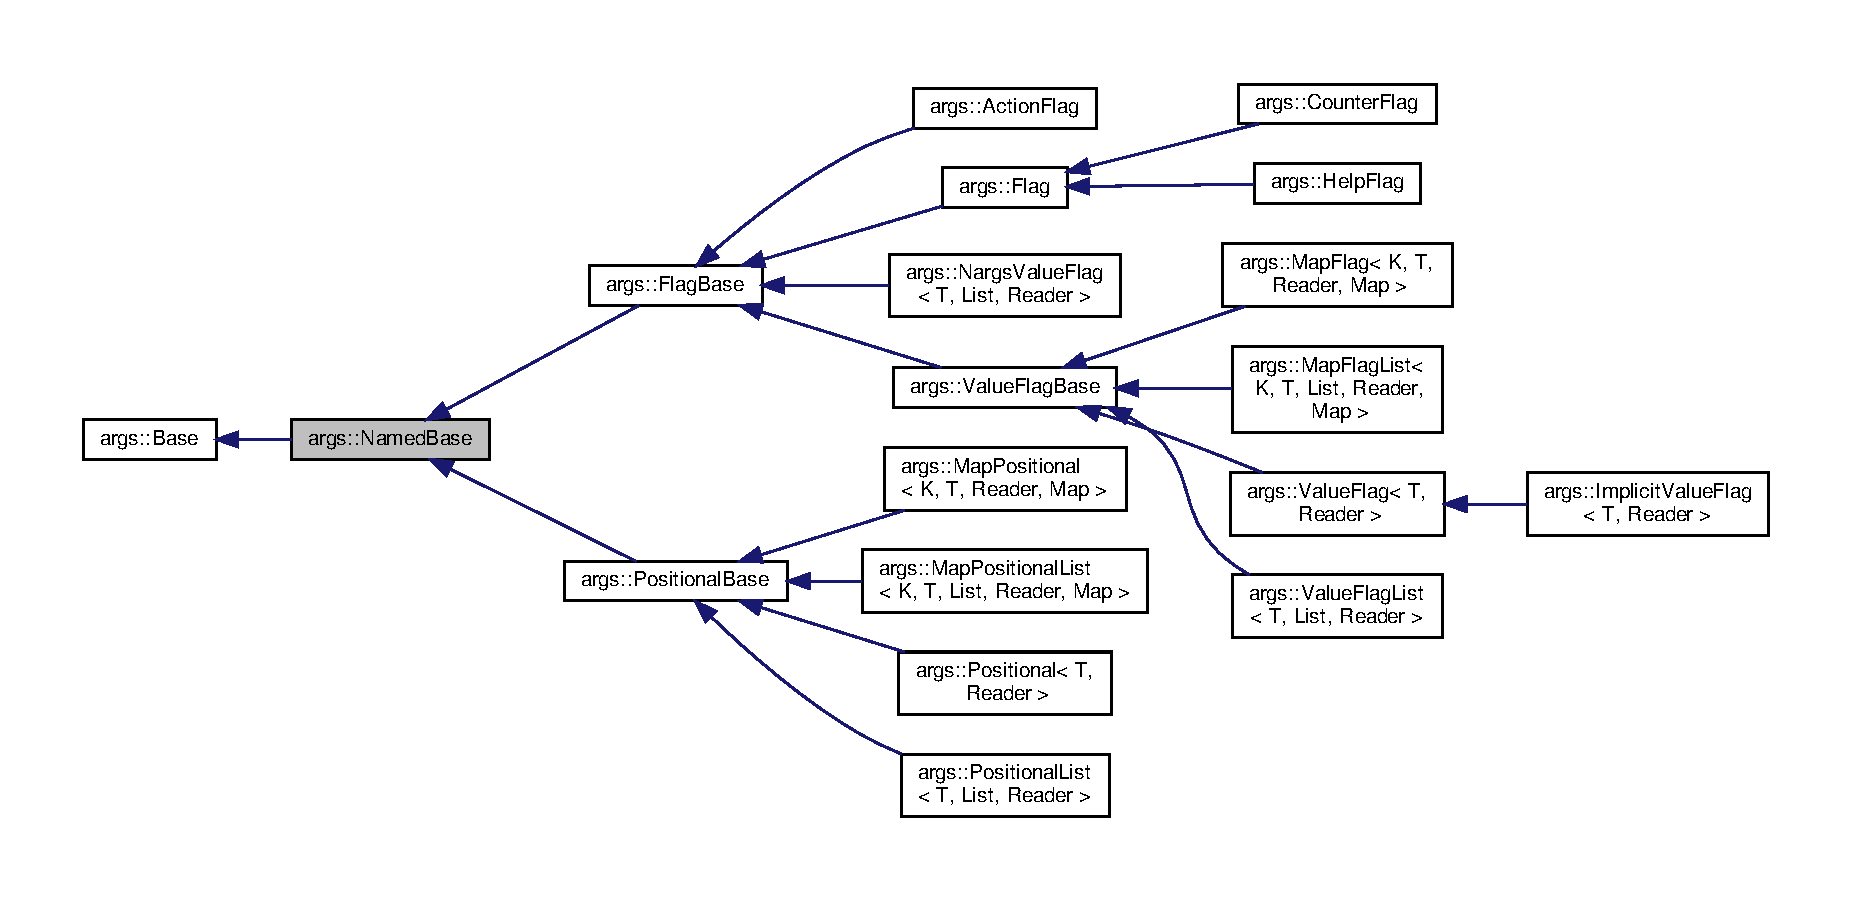
\includegraphics[width=350pt]{classargs_1_1_named_base__inherit__graph}
\end{center}
\end{figure}


Collaboration diagram for args\+:\+:Named\+Base\+:\nopagebreak
\begin{figure}[H]
\begin{center}
\leavevmode
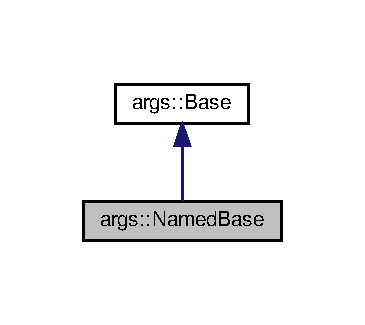
\includegraphics[width=175pt]{classargs_1_1_named_base__coll__graph}
\end{center}
\end{figure}
\subsection*{Public Member Functions}
\begin{DoxyCompactItemize}
\item 
\hyperlink{classargs_1_1_named_base_a09810fc700d6ab589e04f3414edb4f4f}{Named\+Base} (const std\+::string \&name\+\_\+, const std\+::string \&help\+\_\+, \hyperlink{namespaceargs_aa530c0f95194aa275f49a5f299ac9e77}{Options} options\+\_\+=\{\})
\item 
virtual \hyperlink{classargs_1_1_named_base_af4a12e876c93437cd73633bb8255e8eb}{$\sim$\+Named\+Base} ()
\item 
void \hyperlink{classargs_1_1_named_base_a1e94ca498932f60c6e98ba4b88abcc4b}{Help\+Default} (const std\+::string \&str)
\item 
void \hyperlink{classargs_1_1_named_base_a084a776592a24153f1f0aaf28d81f495}{Help\+Choices} (const std\+::string \&str)
\item 
virtual std\+::vector$<$ std\+::tuple$<$ std\+::string, std\+::string, unsigned $>$ $>$ \hyperlink{classargs_1_1_named_base_ab0b9e1f22abf04b24659fada61a6d665}{Get\+Description} (const \hyperlink{structargs_1_1_help_params}{Help\+Params} \&params, const unsigned indent\+Level) const override
\item 
virtual std\+::string \hyperlink{classargs_1_1_named_base_a7e7bab5c0de59e717b87935b14376dfc}{Name} () const
\end{DoxyCompactItemize}
\subsection*{Protected Member Functions}
\begin{DoxyCompactItemize}
\item 
virtual std\+::string \hyperlink{classargs_1_1_named_base_a5866b205907d924423eb8aac9a9e65f8}{Get\+Default\+String} (const \hyperlink{structargs_1_1_help_params}{Help\+Params} \&) const
\item 
virtual std\+::string \hyperlink{classargs_1_1_named_base_aa9104a04001d10c5732a5feb01204cf7}{Get\+Choices\+String} (const \hyperlink{structargs_1_1_help_params}{Help\+Params} \&) const
\item 
virtual std\+::string \hyperlink{classargs_1_1_named_base_a3c597a489d3ccc74937682407c08b3f7}{Get\+Name\+String} (const \hyperlink{structargs_1_1_help_params}{Help\+Params} \&) const
\item 
void \hyperlink{classargs_1_1_named_base_acfaa8c03922fc9b0181a10ca03156e12}{Add\+Description\+Postfix} (std\+::string \&dest, const bool is\+Manual, const std\+::string \&manual, bool is\+Generated, const std\+::string \&generated, const std\+::string \&str) const
\end{DoxyCompactItemize}
\subsection*{Protected Attributes}
\begin{DoxyCompactItemize}
\item 
const std\+::string \hyperlink{classargs_1_1_named_base_a774cbec5dc864c48e84051c044cefa77}{name}
\item 
bool \hyperlink{classargs_1_1_named_base_a034ad347cb530cbf9e0e9ce1b67a66ba}{kickout} = false
\item 
std\+::string \hyperlink{classargs_1_1_named_base_a7460bf500a1873039fc741247a959ddc}{default\+String}
\item 
bool \hyperlink{classargs_1_1_named_base_a2bfe3539152114a52a4a8089920eea59}{default\+String\+Manual} = false
\item 
std\+::string \hyperlink{classargs_1_1_named_base_a2e1624c744d671916b0c943f8fbad962}{choices\+String}
\item 
bool \hyperlink{classargs_1_1_named_base_afc180b62e1f2d9c194354b163f3410b6}{choices\+String\+Manual} = false
\end{DoxyCompactItemize}


\subsection{Detailed Description}
\hyperlink{classargs_1_1_base}{Base} class for all match types that have a name 

\subsection{Constructor \& Destructor Documentation}
\mbox{\Hypertarget{classargs_1_1_named_base_a09810fc700d6ab589e04f3414edb4f4f}\label{classargs_1_1_named_base_a09810fc700d6ab589e04f3414edb4f4f}} 
\index{args\+::\+Named\+Base@{args\+::\+Named\+Base}!Named\+Base@{Named\+Base}}
\index{Named\+Base@{Named\+Base}!args\+::\+Named\+Base@{args\+::\+Named\+Base}}
\subsubsection{\texorpdfstring{Named\+Base()}{NamedBase()}}
{\footnotesize\ttfamily args\+::\+Named\+Base\+::\+Named\+Base (\begin{DoxyParamCaption}\item[{const std\+::string \&}]{name\+\_\+,  }\item[{const std\+::string \&}]{help\+\_\+,  }\item[{\hyperlink{namespaceargs_aa530c0f95194aa275f49a5f299ac9e77}{Options}}]{options\+\_\+ = {\ttfamily \{\}} }\end{DoxyParamCaption})\hspace{0.3cm}{\ttfamily [inline]}}

\mbox{\Hypertarget{classargs_1_1_named_base_af4a12e876c93437cd73633bb8255e8eb}\label{classargs_1_1_named_base_af4a12e876c93437cd73633bb8255e8eb}} 
\index{args\+::\+Named\+Base@{args\+::\+Named\+Base}!````~Named\+Base@{$\sim$\+Named\+Base}}
\index{````~Named\+Base@{$\sim$\+Named\+Base}!args\+::\+Named\+Base@{args\+::\+Named\+Base}}
\subsubsection{\texorpdfstring{$\sim$\+Named\+Base()}{~NamedBase()}}
{\footnotesize\ttfamily virtual args\+::\+Named\+Base\+::$\sim$\+Named\+Base (\begin{DoxyParamCaption}{ }\end{DoxyParamCaption})\hspace{0.3cm}{\ttfamily [inline]}, {\ttfamily [virtual]}}



\subsection{Member Function Documentation}
\mbox{\Hypertarget{classargs_1_1_named_base_acfaa8c03922fc9b0181a10ca03156e12}\label{classargs_1_1_named_base_acfaa8c03922fc9b0181a10ca03156e12}} 
\index{args\+::\+Named\+Base@{args\+::\+Named\+Base}!Add\+Description\+Postfix@{Add\+Description\+Postfix}}
\index{Add\+Description\+Postfix@{Add\+Description\+Postfix}!args\+::\+Named\+Base@{args\+::\+Named\+Base}}
\subsubsection{\texorpdfstring{Add\+Description\+Postfix()}{AddDescriptionPostfix()}}
{\footnotesize\ttfamily void args\+::\+Named\+Base\+::\+Add\+Description\+Postfix (\begin{DoxyParamCaption}\item[{std\+::string \&}]{dest,  }\item[{const bool}]{is\+Manual,  }\item[{const std\+::string \&}]{manual,  }\item[{bool}]{is\+Generated,  }\item[{const std\+::string \&}]{generated,  }\item[{const std\+::string \&}]{str }\end{DoxyParamCaption}) const\hspace{0.3cm}{\ttfamily [inline]}, {\ttfamily [protected]}}

\mbox{\Hypertarget{classargs_1_1_named_base_aa9104a04001d10c5732a5feb01204cf7}\label{classargs_1_1_named_base_aa9104a04001d10c5732a5feb01204cf7}} 
\index{args\+::\+Named\+Base@{args\+::\+Named\+Base}!Get\+Choices\+String@{Get\+Choices\+String}}
\index{Get\+Choices\+String@{Get\+Choices\+String}!args\+::\+Named\+Base@{args\+::\+Named\+Base}}
\subsubsection{\texorpdfstring{Get\+Choices\+String()}{GetChoicesString()}}
{\footnotesize\ttfamily virtual std\+::string args\+::\+Named\+Base\+::\+Get\+Choices\+String (\begin{DoxyParamCaption}\item[{const \hyperlink{structargs_1_1_help_params}{Help\+Params} \&}]{ }\end{DoxyParamCaption}) const\hspace{0.3cm}{\ttfamily [inline]}, {\ttfamily [protected]}, {\ttfamily [virtual]}}



Reimplemented in \hyperlink{classargs_1_1_map_flag_a7fe91b5ef6696b82aa8999884bbf727d}{args\+::\+Map\+Flag$<$ K, T, Reader, Map $>$}.

\mbox{\Hypertarget{classargs_1_1_named_base_a5866b205907d924423eb8aac9a9e65f8}\label{classargs_1_1_named_base_a5866b205907d924423eb8aac9a9e65f8}} 
\index{args\+::\+Named\+Base@{args\+::\+Named\+Base}!Get\+Default\+String@{Get\+Default\+String}}
\index{Get\+Default\+String@{Get\+Default\+String}!args\+::\+Named\+Base@{args\+::\+Named\+Base}}
\subsubsection{\texorpdfstring{Get\+Default\+String()}{GetDefaultString()}}
{\footnotesize\ttfamily virtual std\+::string args\+::\+Named\+Base\+::\+Get\+Default\+String (\begin{DoxyParamCaption}\item[{const \hyperlink{structargs_1_1_help_params}{Help\+Params} \&}]{ }\end{DoxyParamCaption}) const\hspace{0.3cm}{\ttfamily [inline]}, {\ttfamily [protected]}, {\ttfamily [virtual]}}



Reimplemented in \hyperlink{classargs_1_1_value_flag_a47aa01f545a1781583c96af12c8e2062}{args\+::\+Value\+Flag$<$ T, Reader $>$}.

\mbox{\Hypertarget{classargs_1_1_named_base_ab0b9e1f22abf04b24659fada61a6d665}\label{classargs_1_1_named_base_ab0b9e1f22abf04b24659fada61a6d665}} 
\index{args\+::\+Named\+Base@{args\+::\+Named\+Base}!Get\+Description@{Get\+Description}}
\index{Get\+Description@{Get\+Description}!args\+::\+Named\+Base@{args\+::\+Named\+Base}}
\subsubsection{\texorpdfstring{Get\+Description()}{GetDescription()}}
{\footnotesize\ttfamily virtual std\+::vector$<$std\+::tuple$<$std\+::string, std\+::string, unsigned$>$ $>$ args\+::\+Named\+Base\+::\+Get\+Description (\begin{DoxyParamCaption}\item[{const \hyperlink{structargs_1_1_help_params}{Help\+Params} \&}]{params,  }\item[{const unsigned}]{indent\+Level }\end{DoxyParamCaption}) const\hspace{0.3cm}{\ttfamily [inline]}, {\ttfamily [override]}, {\ttfamily [virtual]}}



Reimplemented from \hyperlink{classargs_1_1_base_afbdf4f1ca1f61182ef0461e02e9e9ed3}{args\+::\+Base}.

\mbox{\Hypertarget{classargs_1_1_named_base_a3c597a489d3ccc74937682407c08b3f7}\label{classargs_1_1_named_base_a3c597a489d3ccc74937682407c08b3f7}} 
\index{args\+::\+Named\+Base@{args\+::\+Named\+Base}!Get\+Name\+String@{Get\+Name\+String}}
\index{Get\+Name\+String@{Get\+Name\+String}!args\+::\+Named\+Base@{args\+::\+Named\+Base}}
\subsubsection{\texorpdfstring{Get\+Name\+String()}{GetNameString()}}
{\footnotesize\ttfamily virtual std\+::string args\+::\+Named\+Base\+::\+Get\+Name\+String (\begin{DoxyParamCaption}\item[{const \hyperlink{structargs_1_1_help_params}{Help\+Params} \&}]{ }\end{DoxyParamCaption}) const\hspace{0.3cm}{\ttfamily [inline]}, {\ttfamily [protected]}, {\ttfamily [virtual]}}



Reimplemented in \hyperlink{classargs_1_1_flag_base_a61db383104c1987904bcd331d8b3be76}{args\+::\+Flag\+Base}.

\mbox{\Hypertarget{classargs_1_1_named_base_a084a776592a24153f1f0aaf28d81f495}\label{classargs_1_1_named_base_a084a776592a24153f1f0aaf28d81f495}} 
\index{args\+::\+Named\+Base@{args\+::\+Named\+Base}!Help\+Choices@{Help\+Choices}}
\index{Help\+Choices@{Help\+Choices}!args\+::\+Named\+Base@{args\+::\+Named\+Base}}
\subsubsection{\texorpdfstring{Help\+Choices()}{HelpChoices()}}
{\footnotesize\ttfamily void args\+::\+Named\+Base\+::\+Help\+Choices (\begin{DoxyParamCaption}\item[{const std\+::string \&}]{str }\end{DoxyParamCaption})\hspace{0.3cm}{\ttfamily [inline]}}

Sets choices string that will be added to argument description. Use empty string to disable it for this argument. \mbox{\Hypertarget{classargs_1_1_named_base_a1e94ca498932f60c6e98ba4b88abcc4b}\label{classargs_1_1_named_base_a1e94ca498932f60c6e98ba4b88abcc4b}} 
\index{args\+::\+Named\+Base@{args\+::\+Named\+Base}!Help\+Default@{Help\+Default}}
\index{Help\+Default@{Help\+Default}!args\+::\+Named\+Base@{args\+::\+Named\+Base}}
\subsubsection{\texorpdfstring{Help\+Default()}{HelpDefault()}}
{\footnotesize\ttfamily void args\+::\+Named\+Base\+::\+Help\+Default (\begin{DoxyParamCaption}\item[{const std\+::string \&}]{str }\end{DoxyParamCaption})\hspace{0.3cm}{\ttfamily [inline]}}

Sets default value string that will be added to argument description. Use empty string to disable it for this argument. \mbox{\Hypertarget{classargs_1_1_named_base_a7e7bab5c0de59e717b87935b14376dfc}\label{classargs_1_1_named_base_a7e7bab5c0de59e717b87935b14376dfc}} 
\index{args\+::\+Named\+Base@{args\+::\+Named\+Base}!Name@{Name}}
\index{Name@{Name}!args\+::\+Named\+Base@{args\+::\+Named\+Base}}
\subsubsection{\texorpdfstring{Name()}{Name()}}
{\footnotesize\ttfamily virtual std\+::string args\+::\+Named\+Base\+::\+Name (\begin{DoxyParamCaption}{ }\end{DoxyParamCaption}) const\hspace{0.3cm}{\ttfamily [inline]}, {\ttfamily [virtual]}}



Reimplemented in \hyperlink{classargs_1_1_map_positional_list_a06d9cd19fea86e0027f2ab4a491f19bb}{args\+::\+Map\+Positional\+List$<$ K, T, List, Reader, Map $>$}, \hyperlink{classargs_1_1_positional_list_a5109dbd118c40b6cde570fa37acac950}{args\+::\+Positional\+List$<$ T, List, Reader $>$}, \hyperlink{classargs_1_1_map_flag_list_a1703584ba7b36c5e15aa375eae23903c}{args\+::\+Map\+Flag\+List$<$ K, T, List, Reader, Map $>$}, and \hyperlink{classargs_1_1_value_flag_list_ac0188f5bbc605c02edce2a91675d423c}{args\+::\+Value\+Flag\+List$<$ T, List, Reader $>$}.



\subsection{Member Data Documentation}
\mbox{\Hypertarget{classargs_1_1_named_base_a2e1624c744d671916b0c943f8fbad962}\label{classargs_1_1_named_base_a2e1624c744d671916b0c943f8fbad962}} 
\index{args\+::\+Named\+Base@{args\+::\+Named\+Base}!choices\+String@{choices\+String}}
\index{choices\+String@{choices\+String}!args\+::\+Named\+Base@{args\+::\+Named\+Base}}
\subsubsection{\texorpdfstring{choices\+String}{choicesString}}
{\footnotesize\ttfamily std\+::string args\+::\+Named\+Base\+::choices\+String\hspace{0.3cm}{\ttfamily [protected]}}

\mbox{\Hypertarget{classargs_1_1_named_base_afc180b62e1f2d9c194354b163f3410b6}\label{classargs_1_1_named_base_afc180b62e1f2d9c194354b163f3410b6}} 
\index{args\+::\+Named\+Base@{args\+::\+Named\+Base}!choices\+String\+Manual@{choices\+String\+Manual}}
\index{choices\+String\+Manual@{choices\+String\+Manual}!args\+::\+Named\+Base@{args\+::\+Named\+Base}}
\subsubsection{\texorpdfstring{choices\+String\+Manual}{choicesStringManual}}
{\footnotesize\ttfamily bool args\+::\+Named\+Base\+::choices\+String\+Manual = false\hspace{0.3cm}{\ttfamily [protected]}}

\mbox{\Hypertarget{classargs_1_1_named_base_a7460bf500a1873039fc741247a959ddc}\label{classargs_1_1_named_base_a7460bf500a1873039fc741247a959ddc}} 
\index{args\+::\+Named\+Base@{args\+::\+Named\+Base}!default\+String@{default\+String}}
\index{default\+String@{default\+String}!args\+::\+Named\+Base@{args\+::\+Named\+Base}}
\subsubsection{\texorpdfstring{default\+String}{defaultString}}
{\footnotesize\ttfamily std\+::string args\+::\+Named\+Base\+::default\+String\hspace{0.3cm}{\ttfamily [protected]}}

\mbox{\Hypertarget{classargs_1_1_named_base_a2bfe3539152114a52a4a8089920eea59}\label{classargs_1_1_named_base_a2bfe3539152114a52a4a8089920eea59}} 
\index{args\+::\+Named\+Base@{args\+::\+Named\+Base}!default\+String\+Manual@{default\+String\+Manual}}
\index{default\+String\+Manual@{default\+String\+Manual}!args\+::\+Named\+Base@{args\+::\+Named\+Base}}
\subsubsection{\texorpdfstring{default\+String\+Manual}{defaultStringManual}}
{\footnotesize\ttfamily bool args\+::\+Named\+Base\+::default\+String\+Manual = false\hspace{0.3cm}{\ttfamily [protected]}}

\mbox{\Hypertarget{classargs_1_1_named_base_a034ad347cb530cbf9e0e9ce1b67a66ba}\label{classargs_1_1_named_base_a034ad347cb530cbf9e0e9ce1b67a66ba}} 
\index{args\+::\+Named\+Base@{args\+::\+Named\+Base}!kickout@{kickout}}
\index{kickout@{kickout}!args\+::\+Named\+Base@{args\+::\+Named\+Base}}
\subsubsection{\texorpdfstring{kickout}{kickout}}
{\footnotesize\ttfamily bool args\+::\+Named\+Base\+::kickout = false\hspace{0.3cm}{\ttfamily [protected]}}

\mbox{\Hypertarget{classargs_1_1_named_base_a774cbec5dc864c48e84051c044cefa77}\label{classargs_1_1_named_base_a774cbec5dc864c48e84051c044cefa77}} 
\index{args\+::\+Named\+Base@{args\+::\+Named\+Base}!name@{name}}
\index{name@{name}!args\+::\+Named\+Base@{args\+::\+Named\+Base}}
\subsubsection{\texorpdfstring{name}{name}}
{\footnotesize\ttfamily const std\+::string args\+::\+Named\+Base\+::name\hspace{0.3cm}{\ttfamily [protected]}}



The documentation for this class was generated from the following file\+:\begin{DoxyCompactItemize}
\item 
/home/cappelletto/github/self/landing\+\_\+area\+\_\+detector/external/\hyperlink{args_8hxx}{args.\+hxx}\end{DoxyCompactItemize}

\hypertarget{structargs_1_1_nargs}{}\section{args\+:\+:Nargs Struct Reference}
\label{structargs_1_1_nargs}\index{args\+::\+Nargs@{args\+::\+Nargs}}


{\ttfamily \#include $<$args.\+hxx$>$}

\subsection*{Public Member Functions}
\begin{DoxyCompactItemize}
\item 
\hyperlink{structargs_1_1_nargs_a90438011275ec1ed792dabb6e47d5f05}{Nargs} (size\+\_\+t min\+\_\+, size\+\_\+t max\+\_\+)
\item 
\hyperlink{structargs_1_1_nargs_aed8011e8041269c28e11ebbe36607395}{Nargs} (size\+\_\+t num\+\_\+)
\end{DoxyCompactItemize}
\subsection*{Public Attributes}
\begin{DoxyCompactItemize}
\item 
const size\+\_\+t \hyperlink{structargs_1_1_nargs_accb94d349138f6b760ace606204df756}{min}
\item 
const size\+\_\+t \hyperlink{structargs_1_1_nargs_a03905b656f58dd338a7d65f801694b16}{max}
\end{DoxyCompactItemize}
\subsection*{Friends}
\begin{DoxyCompactItemize}
\item 
bool \hyperlink{structargs_1_1_nargs_ade1401f3b2f06774e60f90614702d930}{operator==} (const \hyperlink{structargs_1_1_nargs}{Nargs} \&lhs, const \hyperlink{structargs_1_1_nargs}{Nargs} \&rhs)
\item 
bool \hyperlink{structargs_1_1_nargs_acf6ad66d603f4d8e782de5833d9360ab}{operator!=} (const \hyperlink{structargs_1_1_nargs}{Nargs} \&lhs, const \hyperlink{structargs_1_1_nargs}{Nargs} \&rhs)
\end{DoxyCompactItemize}


\subsection{Detailed Description}
A number of arguments which can be consumed by an option.

Represents a closed interval \mbox{[}min, max\mbox{]}. 

\subsection{Constructor \& Destructor Documentation}
\mbox{\Hypertarget{structargs_1_1_nargs_a90438011275ec1ed792dabb6e47d5f05}\label{structargs_1_1_nargs_a90438011275ec1ed792dabb6e47d5f05}} 
\index{args\+::\+Nargs@{args\+::\+Nargs}!Nargs@{Nargs}}
\index{Nargs@{Nargs}!args\+::\+Nargs@{args\+::\+Nargs}}
\subsubsection{\texorpdfstring{Nargs()}{Nargs()}\hspace{0.1cm}{\footnotesize\ttfamily [1/2]}}
{\footnotesize\ttfamily args\+::\+Nargs\+::\+Nargs (\begin{DoxyParamCaption}\item[{size\+\_\+t}]{min\+\_\+,  }\item[{size\+\_\+t}]{max\+\_\+ }\end{DoxyParamCaption})\hspace{0.3cm}{\ttfamily [inline]}}

\mbox{\Hypertarget{structargs_1_1_nargs_aed8011e8041269c28e11ebbe36607395}\label{structargs_1_1_nargs_aed8011e8041269c28e11ebbe36607395}} 
\index{args\+::\+Nargs@{args\+::\+Nargs}!Nargs@{Nargs}}
\index{Nargs@{Nargs}!args\+::\+Nargs@{args\+::\+Nargs}}
\subsubsection{\texorpdfstring{Nargs()}{Nargs()}\hspace{0.1cm}{\footnotesize\ttfamily [2/2]}}
{\footnotesize\ttfamily args\+::\+Nargs\+::\+Nargs (\begin{DoxyParamCaption}\item[{size\+\_\+t}]{num\+\_\+ }\end{DoxyParamCaption})\hspace{0.3cm}{\ttfamily [inline]}}



\subsection{Friends And Related Function Documentation}
\mbox{\Hypertarget{structargs_1_1_nargs_acf6ad66d603f4d8e782de5833d9360ab}\label{structargs_1_1_nargs_acf6ad66d603f4d8e782de5833d9360ab}} 
\index{args\+::\+Nargs@{args\+::\+Nargs}!operator"!=@{operator"!=}}
\index{operator"!=@{operator"!=}!args\+::\+Nargs@{args\+::\+Nargs}}
\subsubsection{\texorpdfstring{operator"!=}{operator!=}}
{\footnotesize\ttfamily bool operator!= (\begin{DoxyParamCaption}\item[{const \hyperlink{structargs_1_1_nargs}{Nargs} \&}]{lhs,  }\item[{const \hyperlink{structargs_1_1_nargs}{Nargs} \&}]{rhs }\end{DoxyParamCaption})\hspace{0.3cm}{\ttfamily [friend]}}

\mbox{\Hypertarget{structargs_1_1_nargs_ade1401f3b2f06774e60f90614702d930}\label{structargs_1_1_nargs_ade1401f3b2f06774e60f90614702d930}} 
\index{args\+::\+Nargs@{args\+::\+Nargs}!operator==@{operator==}}
\index{operator==@{operator==}!args\+::\+Nargs@{args\+::\+Nargs}}
\subsubsection{\texorpdfstring{operator==}{operator==}}
{\footnotesize\ttfamily bool operator== (\begin{DoxyParamCaption}\item[{const \hyperlink{structargs_1_1_nargs}{Nargs} \&}]{lhs,  }\item[{const \hyperlink{structargs_1_1_nargs}{Nargs} \&}]{rhs }\end{DoxyParamCaption})\hspace{0.3cm}{\ttfamily [friend]}}



\subsection{Member Data Documentation}
\mbox{\Hypertarget{structargs_1_1_nargs_a03905b656f58dd338a7d65f801694b16}\label{structargs_1_1_nargs_a03905b656f58dd338a7d65f801694b16}} 
\index{args\+::\+Nargs@{args\+::\+Nargs}!max@{max}}
\index{max@{max}!args\+::\+Nargs@{args\+::\+Nargs}}
\subsubsection{\texorpdfstring{max}{max}}
{\footnotesize\ttfamily const size\+\_\+t args\+::\+Nargs\+::max}

\mbox{\Hypertarget{structargs_1_1_nargs_accb94d349138f6b760ace606204df756}\label{structargs_1_1_nargs_accb94d349138f6b760ace606204df756}} 
\index{args\+::\+Nargs@{args\+::\+Nargs}!min@{min}}
\index{min@{min}!args\+::\+Nargs@{args\+::\+Nargs}}
\subsubsection{\texorpdfstring{min}{min}}
{\footnotesize\ttfamily const size\+\_\+t args\+::\+Nargs\+::min}



The documentation for this struct was generated from the following file\+:\begin{DoxyCompactItemize}
\item 
/home/cappelletto/github/self/landing\+\_\+area\+\_\+detector/external/\hyperlink{args_8hxx}{args.\+hxx}\end{DoxyCompactItemize}

\hypertarget{classargs_1_1_nargs_value_flag}{}\section{args\+:\+:Nargs\+Value\+Flag$<$ T, List, Reader $>$ Class Template Reference}
\label{classargs_1_1_nargs_value_flag}\index{args\+::\+Nargs\+Value\+Flag$<$ T, List, Reader $>$@{args\+::\+Nargs\+Value\+Flag$<$ T, List, Reader $>$}}


{\ttfamily \#include $<$args.\+hxx$>$}



Inheritance diagram for args\+:\+:Nargs\+Value\+Flag$<$ T, List, Reader $>$\+:\nopagebreak
\begin{figure}[H]
\begin{center}
\leavevmode
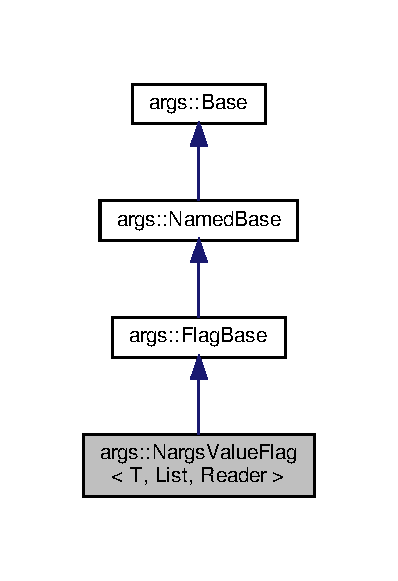
\includegraphics[width=191pt]{classargs_1_1_nargs_value_flag__inherit__graph}
\end{center}
\end{figure}


Collaboration diagram for args\+:\+:Nargs\+Value\+Flag$<$ T, List, Reader $>$\+:\nopagebreak
\begin{figure}[H]
\begin{center}
\leavevmode
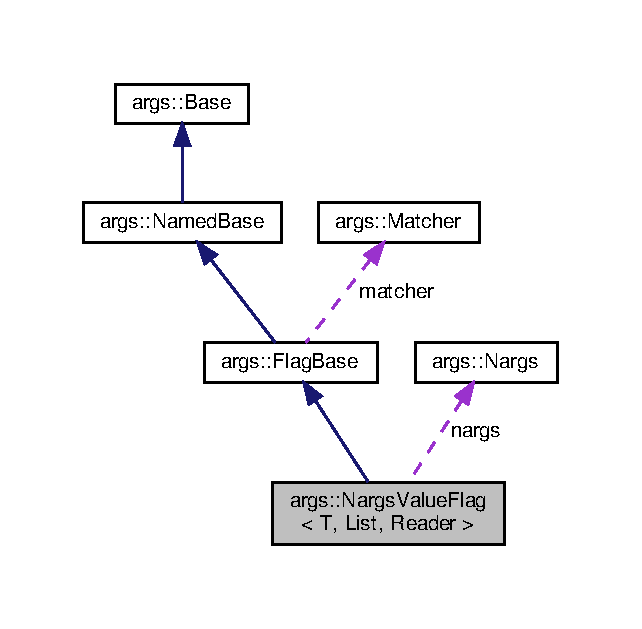
\includegraphics[width=308pt]{classargs_1_1_nargs_value_flag__coll__graph}
\end{center}
\end{figure}
\subsection*{Public Types}
\begin{DoxyCompactItemize}
\item 
typedef List$<$ T $>$ \hyperlink{classargs_1_1_nargs_value_flag_a27e748faa4e5ce69baf05a256e351d42}{Container}
\item 
typedef T \hyperlink{classargs_1_1_nargs_value_flag_a5d1d4da9eeb02c53489608346310af1b}{value\+\_\+type}
\item 
typedef Container\+::allocator\+\_\+type \hyperlink{classargs_1_1_nargs_value_flag_a9c828e4bc64b0037e7e50bb98595a47f}{allocator\+\_\+type}
\item 
typedef Container\+::pointer \hyperlink{classargs_1_1_nargs_value_flag_a3d6171281cd90e7488401a1f86e4a05a}{pointer}
\item 
typedef Container\+::const\+\_\+pointer \hyperlink{classargs_1_1_nargs_value_flag_a7e7d4871821e63a9db65652fa5dda864}{const\+\_\+pointer}
\item 
typedef T \& \hyperlink{classargs_1_1_nargs_value_flag_ab14706e23ffbc72dce81c7eac01e7337}{reference}
\item 
typedef const T \& \hyperlink{classargs_1_1_nargs_value_flag_af8e749af247a14c97883ae90294ef970}{const\+\_\+reference}
\item 
typedef Container\+::size\+\_\+type \hyperlink{classargs_1_1_nargs_value_flag_ad6cb71619fcb40524cf558993549a5cd}{size\+\_\+type}
\item 
typedef Container\+::difference\+\_\+type \hyperlink{classargs_1_1_nargs_value_flag_a889c8ec1eafd60023e417128cd103b18}{difference\+\_\+type}
\item 
typedef Container\+::iterator \hyperlink{classargs_1_1_nargs_value_flag_aeaf17e645a109333204dcb7c954a2473}{iterator}
\item 
typedef Container\+::const\+\_\+iterator \hyperlink{classargs_1_1_nargs_value_flag_a115760faf263d007148b30c99d8e6bdc}{const\+\_\+iterator}
\item 
typedef std\+::reverse\+\_\+iterator$<$ \hyperlink{classargs_1_1_nargs_value_flag_aeaf17e645a109333204dcb7c954a2473}{iterator} $>$ \hyperlink{classargs_1_1_nargs_value_flag_a6fcba5bdf062ce3cc11e25435ec56eae}{reverse\+\_\+iterator}
\item 
typedef std\+::reverse\+\_\+iterator$<$ \hyperlink{classargs_1_1_nargs_value_flag_a115760faf263d007148b30c99d8e6bdc}{const\+\_\+iterator} $>$ \hyperlink{classargs_1_1_nargs_value_flag_a5c004f10973a047ecd2067454e536d41}{const\+\_\+reverse\+\_\+iterator}
\end{DoxyCompactItemize}
\subsection*{Public Member Functions}
\begin{DoxyCompactItemize}
\item 
\hyperlink{classargs_1_1_nargs_value_flag_a49370dd6481756ac2a2177af0068b4bf}{Nargs\+Value\+Flag} (\hyperlink{classargs_1_1_group}{Group} \&group\+\_\+, const std\+::string \&name\+\_\+, const std\+::string \&help\+\_\+, \hyperlink{classargs_1_1_matcher}{Matcher} \&\&matcher\+\_\+, \hyperlink{structargs_1_1_nargs}{Nargs} nargs\+\_\+, const List$<$ T $>$ \&default\+Values\+\_\+=\{\}, \hyperlink{namespaceargs_aa530c0f95194aa275f49a5f299ac9e77}{Options} options\+\_\+=\{\})
\item 
virtual \hyperlink{classargs_1_1_nargs_value_flag_af646d06281e7cb6d453cf36533639601}{$\sim$\+Nargs\+Value\+Flag} ()
\item 
virtual \hyperlink{structargs_1_1_nargs}{Nargs} \hyperlink{classargs_1_1_nargs_value_flag_a8db7ce6ec0d27f649dbfb1bba908078a}{Number\+Of\+Arguments} () const noexcept override
\item 
virtual void \hyperlink{classargs_1_1_nargs_value_flag_aa1ef4abaec468d69c89c02dd8bfdbf38}{Parse\+Value} (const std\+::vector$<$ std\+::string $>$ \&values\+\_\+) override
\item 
List$<$ T $>$ \& \hyperlink{classargs_1_1_nargs_value_flag_ad9789e398db1944fc641153c8742e2c6}{Get} () noexcept
\item 
\hyperlink{classargs_1_1_nargs_value_flag_aeaf17e645a109333204dcb7c954a2473}{iterator} \hyperlink{classargs_1_1_nargs_value_flag_af41b80e20350b97458e4584136311508}{begin} () noexcept
\item 
\hyperlink{classargs_1_1_nargs_value_flag_a115760faf263d007148b30c99d8e6bdc}{const\+\_\+iterator} \hyperlink{classargs_1_1_nargs_value_flag_a72e0031c35bacf86616f1516a1be6fa4}{begin} () const noexcept
\item 
\hyperlink{classargs_1_1_nargs_value_flag_a115760faf263d007148b30c99d8e6bdc}{const\+\_\+iterator} \hyperlink{classargs_1_1_nargs_value_flag_a18231a60382d2992a3fe76686557512f}{cbegin} () const noexcept
\item 
\hyperlink{classargs_1_1_nargs_value_flag_aeaf17e645a109333204dcb7c954a2473}{iterator} \hyperlink{classargs_1_1_nargs_value_flag_afd4a39d8f62aec0daa30674548a30243}{end} () noexcept
\item 
\hyperlink{classargs_1_1_nargs_value_flag_a115760faf263d007148b30c99d8e6bdc}{const\+\_\+iterator} \hyperlink{classargs_1_1_nargs_value_flag_acf5a2440b856c875834abbaf88b8782f}{end} () const noexcept
\item 
\hyperlink{classargs_1_1_nargs_value_flag_a115760faf263d007148b30c99d8e6bdc}{const\+\_\+iterator} \hyperlink{classargs_1_1_nargs_value_flag_a835ee8e007c726d032318c24ac02c0c6}{cend} () const noexcept
\end{DoxyCompactItemize}
\subsection*{Protected Attributes}
\begin{DoxyCompactItemize}
\item 
List$<$ T $>$ \hyperlink{classargs_1_1_nargs_value_flag_ab01fe7ab5b0979e15ce0d2d0896807db}{values}
\item 
\hyperlink{structargs_1_1_nargs}{Nargs} \hyperlink{classargs_1_1_nargs_value_flag_aaf60f389b1e4dc014792e4e515129db5}{nargs}
\item 
Reader \hyperlink{classargs_1_1_nargs_value_flag_a8308b02f086b773b21e588c0e36b6656}{reader}
\end{DoxyCompactItemize}
\subsection*{Additional Inherited Members}


\subsection{Detailed Description}
\subsubsection*{template$<$typename T, template$<$ typename... $>$ class List = std\+::vector, typename Reader = Value\+Reader$>$\newline
class args\+::\+Nargs\+Value\+Flag$<$ T, List, Reader $>$}

A variadic arguments accepting flag class


\begin{DoxyTemplParams}{Template Parameters}
{\em T} & the type to extract the argument as \\
\hline
{\em List} & the list type that houses the values \\
\hline
{\em Reader} & The functor type used to read the argument, taking the name, value, and destination reference with operator(), and returning a bool (if A\+R\+G\+S\+\_\+\+N\+O\+E\+X\+C\+E\+PT is defined) \\
\hline
\end{DoxyTemplParams}


\subsection{Member Typedef Documentation}
\mbox{\Hypertarget{classargs_1_1_nargs_value_flag_a9c828e4bc64b0037e7e50bb98595a47f}\label{classargs_1_1_nargs_value_flag_a9c828e4bc64b0037e7e50bb98595a47f}} 
\index{args\+::\+Nargs\+Value\+Flag@{args\+::\+Nargs\+Value\+Flag}!allocator\+\_\+type@{allocator\+\_\+type}}
\index{allocator\+\_\+type@{allocator\+\_\+type}!args\+::\+Nargs\+Value\+Flag@{args\+::\+Nargs\+Value\+Flag}}
\subsubsection{\texorpdfstring{allocator\+\_\+type}{allocator\_type}}
{\footnotesize\ttfamily template$<$typename T , template$<$ typename... $>$ class List = std\+::vector, typename Reader  = Value\+Reader$>$ \\
typedef Container\+::allocator\+\_\+type \hyperlink{classargs_1_1_nargs_value_flag}{args\+::\+Nargs\+Value\+Flag}$<$ T, List, Reader $>$\+::\hyperlink{classargs_1_1_nargs_value_flag_a9c828e4bc64b0037e7e50bb98595a47f}{allocator\+\_\+type}}

\mbox{\Hypertarget{classargs_1_1_nargs_value_flag_a115760faf263d007148b30c99d8e6bdc}\label{classargs_1_1_nargs_value_flag_a115760faf263d007148b30c99d8e6bdc}} 
\index{args\+::\+Nargs\+Value\+Flag@{args\+::\+Nargs\+Value\+Flag}!const\+\_\+iterator@{const\+\_\+iterator}}
\index{const\+\_\+iterator@{const\+\_\+iterator}!args\+::\+Nargs\+Value\+Flag@{args\+::\+Nargs\+Value\+Flag}}
\subsubsection{\texorpdfstring{const\+\_\+iterator}{const\_iterator}}
{\footnotesize\ttfamily template$<$typename T , template$<$ typename... $>$ class List = std\+::vector, typename Reader  = Value\+Reader$>$ \\
typedef Container\+::const\+\_\+iterator \hyperlink{classargs_1_1_nargs_value_flag}{args\+::\+Nargs\+Value\+Flag}$<$ T, List, Reader $>$\+::\hyperlink{classargs_1_1_nargs_value_flag_a115760faf263d007148b30c99d8e6bdc}{const\+\_\+iterator}}

\mbox{\Hypertarget{classargs_1_1_nargs_value_flag_a7e7d4871821e63a9db65652fa5dda864}\label{classargs_1_1_nargs_value_flag_a7e7d4871821e63a9db65652fa5dda864}} 
\index{args\+::\+Nargs\+Value\+Flag@{args\+::\+Nargs\+Value\+Flag}!const\+\_\+pointer@{const\+\_\+pointer}}
\index{const\+\_\+pointer@{const\+\_\+pointer}!args\+::\+Nargs\+Value\+Flag@{args\+::\+Nargs\+Value\+Flag}}
\subsubsection{\texorpdfstring{const\+\_\+pointer}{const\_pointer}}
{\footnotesize\ttfamily template$<$typename T , template$<$ typename... $>$ class List = std\+::vector, typename Reader  = Value\+Reader$>$ \\
typedef Container\+::const\+\_\+pointer \hyperlink{classargs_1_1_nargs_value_flag}{args\+::\+Nargs\+Value\+Flag}$<$ T, List, Reader $>$\+::\hyperlink{classargs_1_1_nargs_value_flag_a7e7d4871821e63a9db65652fa5dda864}{const\+\_\+pointer}}

\mbox{\Hypertarget{classargs_1_1_nargs_value_flag_af8e749af247a14c97883ae90294ef970}\label{classargs_1_1_nargs_value_flag_af8e749af247a14c97883ae90294ef970}} 
\index{args\+::\+Nargs\+Value\+Flag@{args\+::\+Nargs\+Value\+Flag}!const\+\_\+reference@{const\+\_\+reference}}
\index{const\+\_\+reference@{const\+\_\+reference}!args\+::\+Nargs\+Value\+Flag@{args\+::\+Nargs\+Value\+Flag}}
\subsubsection{\texorpdfstring{const\+\_\+reference}{const\_reference}}
{\footnotesize\ttfamily template$<$typename T , template$<$ typename... $>$ class List = std\+::vector, typename Reader  = Value\+Reader$>$ \\
typedef const T\& \hyperlink{classargs_1_1_nargs_value_flag}{args\+::\+Nargs\+Value\+Flag}$<$ T, List, Reader $>$\+::\hyperlink{classargs_1_1_nargs_value_flag_af8e749af247a14c97883ae90294ef970}{const\+\_\+reference}}

\mbox{\Hypertarget{classargs_1_1_nargs_value_flag_a5c004f10973a047ecd2067454e536d41}\label{classargs_1_1_nargs_value_flag_a5c004f10973a047ecd2067454e536d41}} 
\index{args\+::\+Nargs\+Value\+Flag@{args\+::\+Nargs\+Value\+Flag}!const\+\_\+reverse\+\_\+iterator@{const\+\_\+reverse\+\_\+iterator}}
\index{const\+\_\+reverse\+\_\+iterator@{const\+\_\+reverse\+\_\+iterator}!args\+::\+Nargs\+Value\+Flag@{args\+::\+Nargs\+Value\+Flag}}
\subsubsection{\texorpdfstring{const\+\_\+reverse\+\_\+iterator}{const\_reverse\_iterator}}
{\footnotesize\ttfamily template$<$typename T , template$<$ typename... $>$ class List = std\+::vector, typename Reader  = Value\+Reader$>$ \\
typedef std\+::reverse\+\_\+iterator$<$\hyperlink{classargs_1_1_nargs_value_flag_a115760faf263d007148b30c99d8e6bdc}{const\+\_\+iterator}$>$ \hyperlink{classargs_1_1_nargs_value_flag}{args\+::\+Nargs\+Value\+Flag}$<$ T, List, Reader $>$\+::\hyperlink{classargs_1_1_nargs_value_flag_a5c004f10973a047ecd2067454e536d41}{const\+\_\+reverse\+\_\+iterator}}

\mbox{\Hypertarget{classargs_1_1_nargs_value_flag_a27e748faa4e5ce69baf05a256e351d42}\label{classargs_1_1_nargs_value_flag_a27e748faa4e5ce69baf05a256e351d42}} 
\index{args\+::\+Nargs\+Value\+Flag@{args\+::\+Nargs\+Value\+Flag}!Container@{Container}}
\index{Container@{Container}!args\+::\+Nargs\+Value\+Flag@{args\+::\+Nargs\+Value\+Flag}}
\subsubsection{\texorpdfstring{Container}{Container}}
{\footnotesize\ttfamily template$<$typename T , template$<$ typename... $>$ class List = std\+::vector, typename Reader  = Value\+Reader$>$ \\
typedef List$<$T$>$ \hyperlink{classargs_1_1_nargs_value_flag}{args\+::\+Nargs\+Value\+Flag}$<$ T, List, Reader $>$\+::\hyperlink{classargs_1_1_nargs_value_flag_a27e748faa4e5ce69baf05a256e351d42}{Container}}

\mbox{\Hypertarget{classargs_1_1_nargs_value_flag_a889c8ec1eafd60023e417128cd103b18}\label{classargs_1_1_nargs_value_flag_a889c8ec1eafd60023e417128cd103b18}} 
\index{args\+::\+Nargs\+Value\+Flag@{args\+::\+Nargs\+Value\+Flag}!difference\+\_\+type@{difference\+\_\+type}}
\index{difference\+\_\+type@{difference\+\_\+type}!args\+::\+Nargs\+Value\+Flag@{args\+::\+Nargs\+Value\+Flag}}
\subsubsection{\texorpdfstring{difference\+\_\+type}{difference\_type}}
{\footnotesize\ttfamily template$<$typename T , template$<$ typename... $>$ class List = std\+::vector, typename Reader  = Value\+Reader$>$ \\
typedef Container\+::difference\+\_\+type \hyperlink{classargs_1_1_nargs_value_flag}{args\+::\+Nargs\+Value\+Flag}$<$ T, List, Reader $>$\+::\hyperlink{classargs_1_1_nargs_value_flag_a889c8ec1eafd60023e417128cd103b18}{difference\+\_\+type}}

\mbox{\Hypertarget{classargs_1_1_nargs_value_flag_aeaf17e645a109333204dcb7c954a2473}\label{classargs_1_1_nargs_value_flag_aeaf17e645a109333204dcb7c954a2473}} 
\index{args\+::\+Nargs\+Value\+Flag@{args\+::\+Nargs\+Value\+Flag}!iterator@{iterator}}
\index{iterator@{iterator}!args\+::\+Nargs\+Value\+Flag@{args\+::\+Nargs\+Value\+Flag}}
\subsubsection{\texorpdfstring{iterator}{iterator}}
{\footnotesize\ttfamily template$<$typename T , template$<$ typename... $>$ class List = std\+::vector, typename Reader  = Value\+Reader$>$ \\
typedef Container\+::iterator \hyperlink{classargs_1_1_nargs_value_flag}{args\+::\+Nargs\+Value\+Flag}$<$ T, List, Reader $>$\+::\hyperlink{classargs_1_1_nargs_value_flag_aeaf17e645a109333204dcb7c954a2473}{iterator}}

\mbox{\Hypertarget{classargs_1_1_nargs_value_flag_a3d6171281cd90e7488401a1f86e4a05a}\label{classargs_1_1_nargs_value_flag_a3d6171281cd90e7488401a1f86e4a05a}} 
\index{args\+::\+Nargs\+Value\+Flag@{args\+::\+Nargs\+Value\+Flag}!pointer@{pointer}}
\index{pointer@{pointer}!args\+::\+Nargs\+Value\+Flag@{args\+::\+Nargs\+Value\+Flag}}
\subsubsection{\texorpdfstring{pointer}{pointer}}
{\footnotesize\ttfamily template$<$typename T , template$<$ typename... $>$ class List = std\+::vector, typename Reader  = Value\+Reader$>$ \\
typedef Container\+::pointer \hyperlink{classargs_1_1_nargs_value_flag}{args\+::\+Nargs\+Value\+Flag}$<$ T, List, Reader $>$\+::\hyperlink{classargs_1_1_nargs_value_flag_a3d6171281cd90e7488401a1f86e4a05a}{pointer}}

\mbox{\Hypertarget{classargs_1_1_nargs_value_flag_ab14706e23ffbc72dce81c7eac01e7337}\label{classargs_1_1_nargs_value_flag_ab14706e23ffbc72dce81c7eac01e7337}} 
\index{args\+::\+Nargs\+Value\+Flag@{args\+::\+Nargs\+Value\+Flag}!reference@{reference}}
\index{reference@{reference}!args\+::\+Nargs\+Value\+Flag@{args\+::\+Nargs\+Value\+Flag}}
\subsubsection{\texorpdfstring{reference}{reference}}
{\footnotesize\ttfamily template$<$typename T , template$<$ typename... $>$ class List = std\+::vector, typename Reader  = Value\+Reader$>$ \\
typedef T\& \hyperlink{classargs_1_1_nargs_value_flag}{args\+::\+Nargs\+Value\+Flag}$<$ T, List, Reader $>$\+::\hyperlink{classargs_1_1_nargs_value_flag_ab14706e23ffbc72dce81c7eac01e7337}{reference}}

\mbox{\Hypertarget{classargs_1_1_nargs_value_flag_a6fcba5bdf062ce3cc11e25435ec56eae}\label{classargs_1_1_nargs_value_flag_a6fcba5bdf062ce3cc11e25435ec56eae}} 
\index{args\+::\+Nargs\+Value\+Flag@{args\+::\+Nargs\+Value\+Flag}!reverse\+\_\+iterator@{reverse\+\_\+iterator}}
\index{reverse\+\_\+iterator@{reverse\+\_\+iterator}!args\+::\+Nargs\+Value\+Flag@{args\+::\+Nargs\+Value\+Flag}}
\subsubsection{\texorpdfstring{reverse\+\_\+iterator}{reverse\_iterator}}
{\footnotesize\ttfamily template$<$typename T , template$<$ typename... $>$ class List = std\+::vector, typename Reader  = Value\+Reader$>$ \\
typedef std\+::reverse\+\_\+iterator$<$\hyperlink{classargs_1_1_nargs_value_flag_aeaf17e645a109333204dcb7c954a2473}{iterator}$>$ \hyperlink{classargs_1_1_nargs_value_flag}{args\+::\+Nargs\+Value\+Flag}$<$ T, List, Reader $>$\+::\hyperlink{classargs_1_1_nargs_value_flag_a6fcba5bdf062ce3cc11e25435ec56eae}{reverse\+\_\+iterator}}

\mbox{\Hypertarget{classargs_1_1_nargs_value_flag_ad6cb71619fcb40524cf558993549a5cd}\label{classargs_1_1_nargs_value_flag_ad6cb71619fcb40524cf558993549a5cd}} 
\index{args\+::\+Nargs\+Value\+Flag@{args\+::\+Nargs\+Value\+Flag}!size\+\_\+type@{size\+\_\+type}}
\index{size\+\_\+type@{size\+\_\+type}!args\+::\+Nargs\+Value\+Flag@{args\+::\+Nargs\+Value\+Flag}}
\subsubsection{\texorpdfstring{size\+\_\+type}{size\_type}}
{\footnotesize\ttfamily template$<$typename T , template$<$ typename... $>$ class List = std\+::vector, typename Reader  = Value\+Reader$>$ \\
typedef Container\+::size\+\_\+type \hyperlink{classargs_1_1_nargs_value_flag}{args\+::\+Nargs\+Value\+Flag}$<$ T, List, Reader $>$\+::\hyperlink{classargs_1_1_nargs_value_flag_ad6cb71619fcb40524cf558993549a5cd}{size\+\_\+type}}

\mbox{\Hypertarget{classargs_1_1_nargs_value_flag_a5d1d4da9eeb02c53489608346310af1b}\label{classargs_1_1_nargs_value_flag_a5d1d4da9eeb02c53489608346310af1b}} 
\index{args\+::\+Nargs\+Value\+Flag@{args\+::\+Nargs\+Value\+Flag}!value\+\_\+type@{value\+\_\+type}}
\index{value\+\_\+type@{value\+\_\+type}!args\+::\+Nargs\+Value\+Flag@{args\+::\+Nargs\+Value\+Flag}}
\subsubsection{\texorpdfstring{value\+\_\+type}{value\_type}}
{\footnotesize\ttfamily template$<$typename T , template$<$ typename... $>$ class List = std\+::vector, typename Reader  = Value\+Reader$>$ \\
typedef T \hyperlink{classargs_1_1_nargs_value_flag}{args\+::\+Nargs\+Value\+Flag}$<$ T, List, Reader $>$\+::\hyperlink{classargs_1_1_nargs_value_flag_a5d1d4da9eeb02c53489608346310af1b}{value\+\_\+type}}



\subsection{Constructor \& Destructor Documentation}
\mbox{\Hypertarget{classargs_1_1_nargs_value_flag_a49370dd6481756ac2a2177af0068b4bf}\label{classargs_1_1_nargs_value_flag_a49370dd6481756ac2a2177af0068b4bf}} 
\index{args\+::\+Nargs\+Value\+Flag@{args\+::\+Nargs\+Value\+Flag}!Nargs\+Value\+Flag@{Nargs\+Value\+Flag}}
\index{Nargs\+Value\+Flag@{Nargs\+Value\+Flag}!args\+::\+Nargs\+Value\+Flag@{args\+::\+Nargs\+Value\+Flag}}
\subsubsection{\texorpdfstring{Nargs\+Value\+Flag()}{NargsValueFlag()}}
{\footnotesize\ttfamily template$<$typename T , template$<$ typename... $>$ class List = std\+::vector, typename Reader  = Value\+Reader$>$ \\
\hyperlink{classargs_1_1_nargs_value_flag}{args\+::\+Nargs\+Value\+Flag}$<$ T, List, Reader $>$\+::\hyperlink{classargs_1_1_nargs_value_flag}{Nargs\+Value\+Flag} (\begin{DoxyParamCaption}\item[{\hyperlink{classargs_1_1_group}{Group} \&}]{group\+\_\+,  }\item[{const std\+::string \&}]{name\+\_\+,  }\item[{const std\+::string \&}]{help\+\_\+,  }\item[{\hyperlink{classargs_1_1_matcher}{Matcher} \&\&}]{matcher\+\_\+,  }\item[{\hyperlink{structargs_1_1_nargs}{Nargs}}]{nargs\+\_\+,  }\item[{const List$<$ T $>$ \&}]{default\+Values\+\_\+ = {\ttfamily \{\}},  }\item[{\hyperlink{namespaceargs_aa530c0f95194aa275f49a5f299ac9e77}{Options}}]{options\+\_\+ = {\ttfamily \{\}} }\end{DoxyParamCaption})\hspace{0.3cm}{\ttfamily [inline]}}

\mbox{\Hypertarget{classargs_1_1_nargs_value_flag_af646d06281e7cb6d453cf36533639601}\label{classargs_1_1_nargs_value_flag_af646d06281e7cb6d453cf36533639601}} 
\index{args\+::\+Nargs\+Value\+Flag@{args\+::\+Nargs\+Value\+Flag}!````~Nargs\+Value\+Flag@{$\sim$\+Nargs\+Value\+Flag}}
\index{````~Nargs\+Value\+Flag@{$\sim$\+Nargs\+Value\+Flag}!args\+::\+Nargs\+Value\+Flag@{args\+::\+Nargs\+Value\+Flag}}
\subsubsection{\texorpdfstring{$\sim$\+Nargs\+Value\+Flag()}{~NargsValueFlag()}}
{\footnotesize\ttfamily template$<$typename T , template$<$ typename... $>$ class List = std\+::vector, typename Reader  = Value\+Reader$>$ \\
virtual \hyperlink{classargs_1_1_nargs_value_flag}{args\+::\+Nargs\+Value\+Flag}$<$ T, List, Reader $>$\+::$\sim$\hyperlink{classargs_1_1_nargs_value_flag}{Nargs\+Value\+Flag} (\begin{DoxyParamCaption}{ }\end{DoxyParamCaption})\hspace{0.3cm}{\ttfamily [inline]}, {\ttfamily [virtual]}}



\subsection{Member Function Documentation}
\mbox{\Hypertarget{classargs_1_1_nargs_value_flag_af41b80e20350b97458e4584136311508}\label{classargs_1_1_nargs_value_flag_af41b80e20350b97458e4584136311508}} 
\index{args\+::\+Nargs\+Value\+Flag@{args\+::\+Nargs\+Value\+Flag}!begin@{begin}}
\index{begin@{begin}!args\+::\+Nargs\+Value\+Flag@{args\+::\+Nargs\+Value\+Flag}}
\subsubsection{\texorpdfstring{begin()}{begin()}\hspace{0.1cm}{\footnotesize\ttfamily [1/2]}}
{\footnotesize\ttfamily template$<$typename T , template$<$ typename... $>$ class List = std\+::vector, typename Reader  = Value\+Reader$>$ \\
\hyperlink{classargs_1_1_nargs_value_flag_aeaf17e645a109333204dcb7c954a2473}{iterator} \hyperlink{classargs_1_1_nargs_value_flag}{args\+::\+Nargs\+Value\+Flag}$<$ T, List, Reader $>$\+::begin (\begin{DoxyParamCaption}{ }\end{DoxyParamCaption})\hspace{0.3cm}{\ttfamily [inline]}, {\ttfamily [noexcept]}}

\mbox{\Hypertarget{classargs_1_1_nargs_value_flag_a72e0031c35bacf86616f1516a1be6fa4}\label{classargs_1_1_nargs_value_flag_a72e0031c35bacf86616f1516a1be6fa4}} 
\index{args\+::\+Nargs\+Value\+Flag@{args\+::\+Nargs\+Value\+Flag}!begin@{begin}}
\index{begin@{begin}!args\+::\+Nargs\+Value\+Flag@{args\+::\+Nargs\+Value\+Flag}}
\subsubsection{\texorpdfstring{begin()}{begin()}\hspace{0.1cm}{\footnotesize\ttfamily [2/2]}}
{\footnotesize\ttfamily template$<$typename T , template$<$ typename... $>$ class List = std\+::vector, typename Reader  = Value\+Reader$>$ \\
\hyperlink{classargs_1_1_nargs_value_flag_a115760faf263d007148b30c99d8e6bdc}{const\+\_\+iterator} \hyperlink{classargs_1_1_nargs_value_flag}{args\+::\+Nargs\+Value\+Flag}$<$ T, List, Reader $>$\+::begin (\begin{DoxyParamCaption}{ }\end{DoxyParamCaption}) const\hspace{0.3cm}{\ttfamily [inline]}, {\ttfamily [noexcept]}}

\mbox{\Hypertarget{classargs_1_1_nargs_value_flag_a18231a60382d2992a3fe76686557512f}\label{classargs_1_1_nargs_value_flag_a18231a60382d2992a3fe76686557512f}} 
\index{args\+::\+Nargs\+Value\+Flag@{args\+::\+Nargs\+Value\+Flag}!cbegin@{cbegin}}
\index{cbegin@{cbegin}!args\+::\+Nargs\+Value\+Flag@{args\+::\+Nargs\+Value\+Flag}}
\subsubsection{\texorpdfstring{cbegin()}{cbegin()}}
{\footnotesize\ttfamily template$<$typename T , template$<$ typename... $>$ class List = std\+::vector, typename Reader  = Value\+Reader$>$ \\
\hyperlink{classargs_1_1_nargs_value_flag_a115760faf263d007148b30c99d8e6bdc}{const\+\_\+iterator} \hyperlink{classargs_1_1_nargs_value_flag}{args\+::\+Nargs\+Value\+Flag}$<$ T, List, Reader $>$\+::cbegin (\begin{DoxyParamCaption}{ }\end{DoxyParamCaption}) const\hspace{0.3cm}{\ttfamily [inline]}, {\ttfamily [noexcept]}}

\mbox{\Hypertarget{classargs_1_1_nargs_value_flag_a835ee8e007c726d032318c24ac02c0c6}\label{classargs_1_1_nargs_value_flag_a835ee8e007c726d032318c24ac02c0c6}} 
\index{args\+::\+Nargs\+Value\+Flag@{args\+::\+Nargs\+Value\+Flag}!cend@{cend}}
\index{cend@{cend}!args\+::\+Nargs\+Value\+Flag@{args\+::\+Nargs\+Value\+Flag}}
\subsubsection{\texorpdfstring{cend()}{cend()}}
{\footnotesize\ttfamily template$<$typename T , template$<$ typename... $>$ class List = std\+::vector, typename Reader  = Value\+Reader$>$ \\
\hyperlink{classargs_1_1_nargs_value_flag_a115760faf263d007148b30c99d8e6bdc}{const\+\_\+iterator} \hyperlink{classargs_1_1_nargs_value_flag}{args\+::\+Nargs\+Value\+Flag}$<$ T, List, Reader $>$\+::cend (\begin{DoxyParamCaption}{ }\end{DoxyParamCaption}) const\hspace{0.3cm}{\ttfamily [inline]}, {\ttfamily [noexcept]}}

\mbox{\Hypertarget{classargs_1_1_nargs_value_flag_afd4a39d8f62aec0daa30674548a30243}\label{classargs_1_1_nargs_value_flag_afd4a39d8f62aec0daa30674548a30243}} 
\index{args\+::\+Nargs\+Value\+Flag@{args\+::\+Nargs\+Value\+Flag}!end@{end}}
\index{end@{end}!args\+::\+Nargs\+Value\+Flag@{args\+::\+Nargs\+Value\+Flag}}
\subsubsection{\texorpdfstring{end()}{end()}\hspace{0.1cm}{\footnotesize\ttfamily [1/2]}}
{\footnotesize\ttfamily template$<$typename T , template$<$ typename... $>$ class List = std\+::vector, typename Reader  = Value\+Reader$>$ \\
\hyperlink{classargs_1_1_nargs_value_flag_aeaf17e645a109333204dcb7c954a2473}{iterator} \hyperlink{classargs_1_1_nargs_value_flag}{args\+::\+Nargs\+Value\+Flag}$<$ T, List, Reader $>$\+::end (\begin{DoxyParamCaption}{ }\end{DoxyParamCaption})\hspace{0.3cm}{\ttfamily [inline]}, {\ttfamily [noexcept]}}

\mbox{\Hypertarget{classargs_1_1_nargs_value_flag_acf5a2440b856c875834abbaf88b8782f}\label{classargs_1_1_nargs_value_flag_acf5a2440b856c875834abbaf88b8782f}} 
\index{args\+::\+Nargs\+Value\+Flag@{args\+::\+Nargs\+Value\+Flag}!end@{end}}
\index{end@{end}!args\+::\+Nargs\+Value\+Flag@{args\+::\+Nargs\+Value\+Flag}}
\subsubsection{\texorpdfstring{end()}{end()}\hspace{0.1cm}{\footnotesize\ttfamily [2/2]}}
{\footnotesize\ttfamily template$<$typename T , template$<$ typename... $>$ class List = std\+::vector, typename Reader  = Value\+Reader$>$ \\
\hyperlink{classargs_1_1_nargs_value_flag_a115760faf263d007148b30c99d8e6bdc}{const\+\_\+iterator} \hyperlink{classargs_1_1_nargs_value_flag}{args\+::\+Nargs\+Value\+Flag}$<$ T, List, Reader $>$\+::end (\begin{DoxyParamCaption}{ }\end{DoxyParamCaption}) const\hspace{0.3cm}{\ttfamily [inline]}, {\ttfamily [noexcept]}}

\mbox{\Hypertarget{classargs_1_1_nargs_value_flag_ad9789e398db1944fc641153c8742e2c6}\label{classargs_1_1_nargs_value_flag_ad9789e398db1944fc641153c8742e2c6}} 
\index{args\+::\+Nargs\+Value\+Flag@{args\+::\+Nargs\+Value\+Flag}!Get@{Get}}
\index{Get@{Get}!args\+::\+Nargs\+Value\+Flag@{args\+::\+Nargs\+Value\+Flag}}
\subsubsection{\texorpdfstring{Get()}{Get()}}
{\footnotesize\ttfamily template$<$typename T , template$<$ typename... $>$ class List = std\+::vector, typename Reader  = Value\+Reader$>$ \\
List$<$T$>$\& \hyperlink{classargs_1_1_nargs_value_flag}{args\+::\+Nargs\+Value\+Flag}$<$ T, List, Reader $>$\+::Get (\begin{DoxyParamCaption}{ }\end{DoxyParamCaption})\hspace{0.3cm}{\ttfamily [inline]}, {\ttfamily [noexcept]}}

\mbox{\Hypertarget{classargs_1_1_nargs_value_flag_a8db7ce6ec0d27f649dbfb1bba908078a}\label{classargs_1_1_nargs_value_flag_a8db7ce6ec0d27f649dbfb1bba908078a}} 
\index{args\+::\+Nargs\+Value\+Flag@{args\+::\+Nargs\+Value\+Flag}!Number\+Of\+Arguments@{Number\+Of\+Arguments}}
\index{Number\+Of\+Arguments@{Number\+Of\+Arguments}!args\+::\+Nargs\+Value\+Flag@{args\+::\+Nargs\+Value\+Flag}}
\subsubsection{\texorpdfstring{Number\+Of\+Arguments()}{NumberOfArguments()}}
{\footnotesize\ttfamily template$<$typename T , template$<$ typename... $>$ class List = std\+::vector, typename Reader  = Value\+Reader$>$ \\
virtual \hyperlink{structargs_1_1_nargs}{Nargs} \hyperlink{classargs_1_1_nargs_value_flag}{args\+::\+Nargs\+Value\+Flag}$<$ T, List, Reader $>$\+::Number\+Of\+Arguments (\begin{DoxyParamCaption}{ }\end{DoxyParamCaption}) const\hspace{0.3cm}{\ttfamily [inline]}, {\ttfamily [override]}, {\ttfamily [virtual]}, {\ttfamily [noexcept]}}

Defines how many values can be consumed by this option.

\begin{DoxyReturn}{Returns}
closed interval \mbox{[}min, max\mbox{]} 
\end{DoxyReturn}


Implements \hyperlink{classargs_1_1_flag_base_a6007ffeaa767893cb8eff5333d61673b}{args\+::\+Flag\+Base}.

\mbox{\Hypertarget{classargs_1_1_nargs_value_flag_aa1ef4abaec468d69c89c02dd8bfdbf38}\label{classargs_1_1_nargs_value_flag_aa1ef4abaec468d69c89c02dd8bfdbf38}} 
\index{args\+::\+Nargs\+Value\+Flag@{args\+::\+Nargs\+Value\+Flag}!Parse\+Value@{Parse\+Value}}
\index{Parse\+Value@{Parse\+Value}!args\+::\+Nargs\+Value\+Flag@{args\+::\+Nargs\+Value\+Flag}}
\subsubsection{\texorpdfstring{Parse\+Value()}{ParseValue()}}
{\footnotesize\ttfamily template$<$typename T , template$<$ typename... $>$ class List = std\+::vector, typename Reader  = Value\+Reader$>$ \\
virtual void \hyperlink{classargs_1_1_nargs_value_flag}{args\+::\+Nargs\+Value\+Flag}$<$ T, List, Reader $>$\+::Parse\+Value (\begin{DoxyParamCaption}\item[{const std\+::vector$<$ std\+::string $>$ \&}]{value }\end{DoxyParamCaption})\hspace{0.3cm}{\ttfamily [inline]}, {\ttfamily [override]}, {\ttfamily [virtual]}}

Parse values of this option.


\begin{DoxyParams}{Parameters}
{\em value} & Vector of values. It\textquotesingle{}s size must be in \hyperlink{classargs_1_1_nargs_value_flag_a8db7ce6ec0d27f649dbfb1bba908078a}{Number\+Of\+Arguments()} interval. \\
\hline
\end{DoxyParams}


Implements \hyperlink{classargs_1_1_flag_base_a3421d9a595c9426dc73f62604cdee84f}{args\+::\+Flag\+Base}.



\subsection{Member Data Documentation}
\mbox{\Hypertarget{classargs_1_1_nargs_value_flag_aaf60f389b1e4dc014792e4e515129db5}\label{classargs_1_1_nargs_value_flag_aaf60f389b1e4dc014792e4e515129db5}} 
\index{args\+::\+Nargs\+Value\+Flag@{args\+::\+Nargs\+Value\+Flag}!nargs@{nargs}}
\index{nargs@{nargs}!args\+::\+Nargs\+Value\+Flag@{args\+::\+Nargs\+Value\+Flag}}
\subsubsection{\texorpdfstring{nargs}{nargs}}
{\footnotesize\ttfamily template$<$typename T , template$<$ typename... $>$ class List = std\+::vector, typename Reader  = Value\+Reader$>$ \\
\hyperlink{structargs_1_1_nargs}{Nargs} \hyperlink{classargs_1_1_nargs_value_flag}{args\+::\+Nargs\+Value\+Flag}$<$ T, List, Reader $>$\+::nargs\hspace{0.3cm}{\ttfamily [protected]}}

\mbox{\Hypertarget{classargs_1_1_nargs_value_flag_a8308b02f086b773b21e588c0e36b6656}\label{classargs_1_1_nargs_value_flag_a8308b02f086b773b21e588c0e36b6656}} 
\index{args\+::\+Nargs\+Value\+Flag@{args\+::\+Nargs\+Value\+Flag}!reader@{reader}}
\index{reader@{reader}!args\+::\+Nargs\+Value\+Flag@{args\+::\+Nargs\+Value\+Flag}}
\subsubsection{\texorpdfstring{reader}{reader}}
{\footnotesize\ttfamily template$<$typename T , template$<$ typename... $>$ class List = std\+::vector, typename Reader  = Value\+Reader$>$ \\
Reader \hyperlink{classargs_1_1_nargs_value_flag}{args\+::\+Nargs\+Value\+Flag}$<$ T, List, Reader $>$\+::reader\hspace{0.3cm}{\ttfamily [protected]}}

\mbox{\Hypertarget{classargs_1_1_nargs_value_flag_ab01fe7ab5b0979e15ce0d2d0896807db}\label{classargs_1_1_nargs_value_flag_ab01fe7ab5b0979e15ce0d2d0896807db}} 
\index{args\+::\+Nargs\+Value\+Flag@{args\+::\+Nargs\+Value\+Flag}!values@{values}}
\index{values@{values}!args\+::\+Nargs\+Value\+Flag@{args\+::\+Nargs\+Value\+Flag}}
\subsubsection{\texorpdfstring{values}{values}}
{\footnotesize\ttfamily template$<$typename T , template$<$ typename... $>$ class List = std\+::vector, typename Reader  = Value\+Reader$>$ \\
List$<$T$>$ \hyperlink{classargs_1_1_nargs_value_flag}{args\+::\+Nargs\+Value\+Flag}$<$ T, List, Reader $>$\+::values\hspace{0.3cm}{\ttfamily [protected]}}



The documentation for this class was generated from the following file\+:\begin{DoxyCompactItemize}
\item 
/home/cappelletto/github/self/landing\+\_\+area\+\_\+detector/external/\hyperlink{args_8hxx}{args.\+hxx}\end{DoxyCompactItemize}

\hypertarget{classargs_1_1_parse_error}{}\section{args\+:\+:Parse\+Error Class Reference}
\label{classargs_1_1_parse_error}\index{args\+::\+Parse\+Error@{args\+::\+Parse\+Error}}


{\ttfamily \#include $<$args.\+hxx$>$}



Inheritance diagram for args\+:\+:Parse\+Error\+:\nopagebreak
\begin{figure}[H]
\begin{center}
\leavevmode
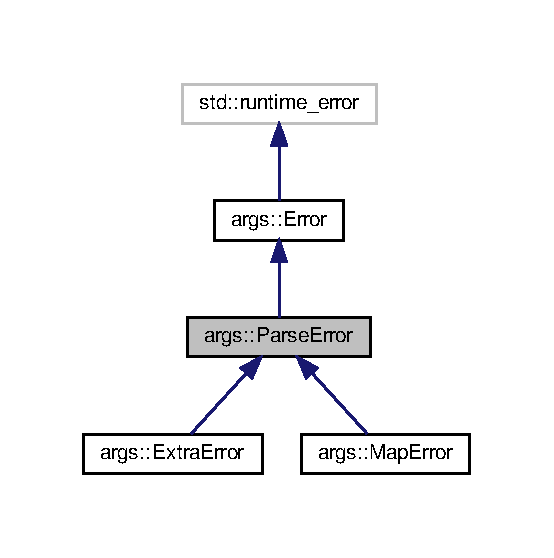
\includegraphics[width=266pt]{classargs_1_1_parse_error__inherit__graph}
\end{center}
\end{figure}


Collaboration diagram for args\+:\+:Parse\+Error\+:\nopagebreak
\begin{figure}[H]
\begin{center}
\leavevmode
\includegraphics[width=173pt]{classargs_1_1_parse_error__coll__graph}
\end{center}
\end{figure}
\subsection*{Public Member Functions}
\begin{DoxyCompactItemize}
\item 
\hyperlink{classargs_1_1_parse_error_a2572276d366705894262de5d8bfd5091}{Parse\+Error} (const std\+::string \&problem)
\item 
virtual \hyperlink{classargs_1_1_parse_error_a8c636a5a068f3fc5bfa3ae5ed17c7a09}{$\sim$\+Parse\+Error} ()
\end{DoxyCompactItemize}


\subsection{Detailed Description}
Errors that occur during regular parsing 

\subsection{Constructor \& Destructor Documentation}
\mbox{\Hypertarget{classargs_1_1_parse_error_a2572276d366705894262de5d8bfd5091}\label{classargs_1_1_parse_error_a2572276d366705894262de5d8bfd5091}} 
\index{args\+::\+Parse\+Error@{args\+::\+Parse\+Error}!Parse\+Error@{Parse\+Error}}
\index{Parse\+Error@{Parse\+Error}!args\+::\+Parse\+Error@{args\+::\+Parse\+Error}}
\subsubsection{\texorpdfstring{Parse\+Error()}{ParseError()}}
{\footnotesize\ttfamily args\+::\+Parse\+Error\+::\+Parse\+Error (\begin{DoxyParamCaption}\item[{const std\+::string \&}]{problem }\end{DoxyParamCaption})\hspace{0.3cm}{\ttfamily [inline]}}

\mbox{\Hypertarget{classargs_1_1_parse_error_a8c636a5a068f3fc5bfa3ae5ed17c7a09}\label{classargs_1_1_parse_error_a8c636a5a068f3fc5bfa3ae5ed17c7a09}} 
\index{args\+::\+Parse\+Error@{args\+::\+Parse\+Error}!````~Parse\+Error@{$\sim$\+Parse\+Error}}
\index{````~Parse\+Error@{$\sim$\+Parse\+Error}!args\+::\+Parse\+Error@{args\+::\+Parse\+Error}}
\subsubsection{\texorpdfstring{$\sim$\+Parse\+Error()}{~ParseError()}}
{\footnotesize\ttfamily virtual args\+::\+Parse\+Error\+::$\sim$\+Parse\+Error (\begin{DoxyParamCaption}{ }\end{DoxyParamCaption})\hspace{0.3cm}{\ttfamily [inline]}, {\ttfamily [virtual]}}



The documentation for this class was generated from the following file\+:\begin{DoxyCompactItemize}
\item 
/home/cappelletto/github/self/landing\+\_\+area\+\_\+detector/external/\hyperlink{args_8hxx}{args.\+hxx}\end{DoxyCompactItemize}

\hypertarget{classargs_1_1_positional}{}\section{args\+:\+:Positional$<$ T, Reader $>$ Class Template Reference}
\label{classargs_1_1_positional}\index{args\+::\+Positional$<$ T, Reader $>$@{args\+::\+Positional$<$ T, Reader $>$}}


{\ttfamily \#include $<$args.\+hxx$>$}



Inheritance diagram for args\+:\+:Positional$<$ T, Reader $>$\+:\nopagebreak
\begin{figure}[H]
\begin{center}
\leavevmode
\includegraphics[width=187pt]{classargs_1_1_positional__inherit__graph}
\end{center}
\end{figure}


Collaboration diagram for args\+:\+:Positional$<$ T, Reader $>$\+:\nopagebreak
\begin{figure}[H]
\begin{center}
\leavevmode
\includegraphics[width=187pt]{classargs_1_1_positional__coll__graph}
\end{center}
\end{figure}
\subsection*{Public Member Functions}
\begin{DoxyCompactItemize}
\item 
\hyperlink{classargs_1_1_positional_ab28805fe2f9364bf9fb2e5f5acf3236d}{Positional} (\hyperlink{classargs_1_1_group}{Group} \&group\+\_\+, const std\+::string \&name\+\_\+, const std\+::string \&help\+\_\+, const T \&default\+Value\+\_\+=T(), \hyperlink{namespaceargs_aa530c0f95194aa275f49a5f299ac9e77}{Options} options\+\_\+=\hyperlink{namespaceargs_aa530c0f95194aa275f49a5f299ac9e77a6adf97f83acf6453d4a6a4b1070f3754}{Options\+::\+None})
\item 
\hyperlink{classargs_1_1_positional_a72a7d74c1578cbc6d7ec0d654a0b001a}{Positional} (\hyperlink{classargs_1_1_group}{Group} \&group\+\_\+, const std\+::string \&name\+\_\+, const std\+::string \&help\+\_\+, \hyperlink{namespaceargs_aa530c0f95194aa275f49a5f299ac9e77}{Options} options\+\_\+)
\item 
virtual \hyperlink{classargs_1_1_positional_a7bf17b3ebdd71316d365df1b225d01d5}{$\sim$\+Positional} ()
\item 
virtual void \hyperlink{classargs_1_1_positional_a2ae24a17caca2e02b95f0977783fc65d}{Parse\+Value} (const std\+::string \&value\+\_\+) override
\item 
T \& \hyperlink{classargs_1_1_positional_ad96c622414ac070fe2ac95363ee1810a}{Get} () noexcept
\end{DoxyCompactItemize}
\subsection*{Additional Inherited Members}


\subsection{Detailed Description}
\subsubsection*{template$<$typename T, typename Reader = Value\+Reader$>$\newline
class args\+::\+Positional$<$ T, Reader $>$}

A positional argument class


\begin{DoxyTemplParams}{Template Parameters}
{\em T} & the type to extract the argument as \\
\hline
{\em Reader} & The functor type used to read the argument, taking the name, value, and destination reference with operator(), and returning a bool (if A\+R\+G\+S\+\_\+\+N\+O\+E\+X\+C\+E\+PT is defined) \\
\hline
\end{DoxyTemplParams}


\subsection{Constructor \& Destructor Documentation}
\mbox{\Hypertarget{classargs_1_1_positional_ab28805fe2f9364bf9fb2e5f5acf3236d}\label{classargs_1_1_positional_ab28805fe2f9364bf9fb2e5f5acf3236d}} 
\index{args\+::\+Positional@{args\+::\+Positional}!Positional@{Positional}}
\index{Positional@{Positional}!args\+::\+Positional@{args\+::\+Positional}}
\subsubsection{\texorpdfstring{Positional()}{Positional()}\hspace{0.1cm}{\footnotesize\ttfamily [1/2]}}
{\footnotesize\ttfamily template$<$typename T , typename Reader  = Value\+Reader$>$ \\
\hyperlink{classargs_1_1_positional}{args\+::\+Positional}$<$ T, Reader $>$\+::\hyperlink{classargs_1_1_positional}{Positional} (\begin{DoxyParamCaption}\item[{\hyperlink{classargs_1_1_group}{Group} \&}]{group\+\_\+,  }\item[{const std\+::string \&}]{name\+\_\+,  }\item[{const std\+::string \&}]{help\+\_\+,  }\item[{const T \&}]{default\+Value\+\_\+ = {\ttfamily T()},  }\item[{\hyperlink{namespaceargs_aa530c0f95194aa275f49a5f299ac9e77}{Options}}]{options\+\_\+ = {\ttfamily \hyperlink{namespaceargs_aa530c0f95194aa275f49a5f299ac9e77a6adf97f83acf6453d4a6a4b1070f3754}{Options\+::\+None}} }\end{DoxyParamCaption})\hspace{0.3cm}{\ttfamily [inline]}}

\mbox{\Hypertarget{classargs_1_1_positional_a72a7d74c1578cbc6d7ec0d654a0b001a}\label{classargs_1_1_positional_a72a7d74c1578cbc6d7ec0d654a0b001a}} 
\index{args\+::\+Positional@{args\+::\+Positional}!Positional@{Positional}}
\index{Positional@{Positional}!args\+::\+Positional@{args\+::\+Positional}}
\subsubsection{\texorpdfstring{Positional()}{Positional()}\hspace{0.1cm}{\footnotesize\ttfamily [2/2]}}
{\footnotesize\ttfamily template$<$typename T , typename Reader  = Value\+Reader$>$ \\
\hyperlink{classargs_1_1_positional}{args\+::\+Positional}$<$ T, Reader $>$\+::\hyperlink{classargs_1_1_positional}{Positional} (\begin{DoxyParamCaption}\item[{\hyperlink{classargs_1_1_group}{Group} \&}]{group\+\_\+,  }\item[{const std\+::string \&}]{name\+\_\+,  }\item[{const std\+::string \&}]{help\+\_\+,  }\item[{\hyperlink{namespaceargs_aa530c0f95194aa275f49a5f299ac9e77}{Options}}]{options\+\_\+ }\end{DoxyParamCaption})\hspace{0.3cm}{\ttfamily [inline]}}

\mbox{\Hypertarget{classargs_1_1_positional_a7bf17b3ebdd71316d365df1b225d01d5}\label{classargs_1_1_positional_a7bf17b3ebdd71316d365df1b225d01d5}} 
\index{args\+::\+Positional@{args\+::\+Positional}!````~Positional@{$\sim$\+Positional}}
\index{````~Positional@{$\sim$\+Positional}!args\+::\+Positional@{args\+::\+Positional}}
\subsubsection{\texorpdfstring{$\sim$\+Positional()}{~Positional()}}
{\footnotesize\ttfamily template$<$typename T , typename Reader  = Value\+Reader$>$ \\
virtual \hyperlink{classargs_1_1_positional}{args\+::\+Positional}$<$ T, Reader $>$\+::$\sim$\hyperlink{classargs_1_1_positional}{Positional} (\begin{DoxyParamCaption}{ }\end{DoxyParamCaption})\hspace{0.3cm}{\ttfamily [inline]}, {\ttfamily [virtual]}}



\subsection{Member Function Documentation}
\mbox{\Hypertarget{classargs_1_1_positional_ad96c622414ac070fe2ac95363ee1810a}\label{classargs_1_1_positional_ad96c622414ac070fe2ac95363ee1810a}} 
\index{args\+::\+Positional@{args\+::\+Positional}!Get@{Get}}
\index{Get@{Get}!args\+::\+Positional@{args\+::\+Positional}}
\subsubsection{\texorpdfstring{Get()}{Get()}}
{\footnotesize\ttfamily template$<$typename T , typename Reader  = Value\+Reader$>$ \\
T\& \hyperlink{classargs_1_1_positional}{args\+::\+Positional}$<$ T, Reader $>$\+::Get (\begin{DoxyParamCaption}{ }\end{DoxyParamCaption})\hspace{0.3cm}{\ttfamily [inline]}, {\ttfamily [noexcept]}}

Get the value \mbox{\Hypertarget{classargs_1_1_positional_a2ae24a17caca2e02b95f0977783fc65d}\label{classargs_1_1_positional_a2ae24a17caca2e02b95f0977783fc65d}} 
\index{args\+::\+Positional@{args\+::\+Positional}!Parse\+Value@{Parse\+Value}}
\index{Parse\+Value@{Parse\+Value}!args\+::\+Positional@{args\+::\+Positional}}
\subsubsection{\texorpdfstring{Parse\+Value()}{ParseValue()}}
{\footnotesize\ttfamily template$<$typename T , typename Reader  = Value\+Reader$>$ \\
virtual void \hyperlink{classargs_1_1_positional}{args\+::\+Positional}$<$ T, Reader $>$\+::Parse\+Value (\begin{DoxyParamCaption}\item[{const std\+::string \&}]{value\+\_\+ }\end{DoxyParamCaption})\hspace{0.3cm}{\ttfamily [inline]}, {\ttfamily [override]}, {\ttfamily [virtual]}}



Implements \hyperlink{classargs_1_1_positional_base_a10b6b91155f56bc28ca25fa87c6f0985}{args\+::\+Positional\+Base}.



The documentation for this class was generated from the following file\+:\begin{DoxyCompactItemize}
\item 
/home/cappelletto/github/self/landing\+\_\+area\+\_\+detector/external/\hyperlink{args_8hxx}{args.\+hxx}\end{DoxyCompactItemize}

\hypertarget{classargs_1_1_positional_base}{}\section{args\+:\+:Positional\+Base Class Reference}
\label{classargs_1_1_positional_base}\index{args\+::\+Positional\+Base@{args\+::\+Positional\+Base}}


{\ttfamily \#include $<$args.\+hxx$>$}



Inheritance diagram for args\+:\+:Positional\+Base\+:\nopagebreak
\begin{figure}[H]
\begin{center}
\leavevmode
\includegraphics[width=350pt]{classargs_1_1_positional_base__inherit__graph}
\end{center}
\end{figure}


Collaboration diagram for args\+:\+:Positional\+Base\+:\nopagebreak
\begin{figure}[H]
\begin{center}
\leavevmode
\includegraphics[width=187pt]{classargs_1_1_positional_base__coll__graph}
\end{center}
\end{figure}
\subsection*{Public Member Functions}
\begin{DoxyCompactItemize}
\item 
\hyperlink{classargs_1_1_positional_base_a767aa51d8d20a299cd369838818d82ab}{Positional\+Base} (const std\+::string \&name\+\_\+, const std\+::string \&help\+\_\+, \hyperlink{namespaceargs_aa530c0f95194aa275f49a5f299ac9e77}{Options} options\+\_\+=\hyperlink{namespaceargs_aa530c0f95194aa275f49a5f299ac9e77a6adf97f83acf6453d4a6a4b1070f3754}{Options\+::\+None})
\item 
virtual \hyperlink{classargs_1_1_positional_base_ae6f5c9ced2da31d6818a6cfb472a063a}{$\sim$\+Positional\+Base} ()
\item 
bool \hyperlink{classargs_1_1_positional_base_a196ab167914517cb9f97b731c3471c19}{Ready} ()
\item 
virtual void \hyperlink{classargs_1_1_positional_base_a10b6b91155f56bc28ca25fa87c6f0985}{Parse\+Value} (const std\+::string \&value\+\_\+)=0
\item 
virtual void \hyperlink{classargs_1_1_positional_base_a14edfb214858983cf5116c8d0fec72ea}{Reset} () noexcept override
\item 
virtual \hyperlink{classargs_1_1_positional_base}{Positional\+Base} $\ast$ \hyperlink{classargs_1_1_positional_base_aaaf09006fd551306b979ea026c49bddb}{Get\+Next\+Positional} () override
\item 
virtual bool \hyperlink{classargs_1_1_positional_base_ad730bb355966fa423046bef31015fbc3}{Has\+Positional} () const override
\item 
virtual std\+::vector$<$ std\+::string $>$ \hyperlink{classargs_1_1_positional_base_a5bf0bc66f4b8cc5aa414fe8976ab8129}{Get\+Program\+Line} (const \hyperlink{structargs_1_1_help_params}{Help\+Params} \&params) const override
\item 
virtual void \hyperlink{classargs_1_1_positional_base_ae328a7b091e6a409df34309a2fb44a71}{Validate} (const std\+::string \&, const std\+::string \&) const override
\end{DoxyCompactItemize}
\subsection*{Protected Attributes}
\begin{DoxyCompactItemize}
\item 
bool \hyperlink{classargs_1_1_positional_base_a3c1226976201c0c62cbd63c5da0a401e}{ready}
\end{DoxyCompactItemize}
\subsection*{Additional Inherited Members}


\subsection{Detailed Description}
\hyperlink{classargs_1_1_base}{Base} class for positional options 

\subsection{Constructor \& Destructor Documentation}
\mbox{\Hypertarget{classargs_1_1_positional_base_a767aa51d8d20a299cd369838818d82ab}\label{classargs_1_1_positional_base_a767aa51d8d20a299cd369838818d82ab}} 
\index{args\+::\+Positional\+Base@{args\+::\+Positional\+Base}!Positional\+Base@{Positional\+Base}}
\index{Positional\+Base@{Positional\+Base}!args\+::\+Positional\+Base@{args\+::\+Positional\+Base}}
\subsubsection{\texorpdfstring{Positional\+Base()}{PositionalBase()}}
{\footnotesize\ttfamily args\+::\+Positional\+Base\+::\+Positional\+Base (\begin{DoxyParamCaption}\item[{const std\+::string \&}]{name\+\_\+,  }\item[{const std\+::string \&}]{help\+\_\+,  }\item[{\hyperlink{namespaceargs_aa530c0f95194aa275f49a5f299ac9e77}{Options}}]{options\+\_\+ = {\ttfamily \hyperlink{namespaceargs_aa530c0f95194aa275f49a5f299ac9e77a6adf97f83acf6453d4a6a4b1070f3754}{Options\+::\+None}} }\end{DoxyParamCaption})\hspace{0.3cm}{\ttfamily [inline]}}

\mbox{\Hypertarget{classargs_1_1_positional_base_ae6f5c9ced2da31d6818a6cfb472a063a}\label{classargs_1_1_positional_base_ae6f5c9ced2da31d6818a6cfb472a063a}} 
\index{args\+::\+Positional\+Base@{args\+::\+Positional\+Base}!````~Positional\+Base@{$\sim$\+Positional\+Base}}
\index{````~Positional\+Base@{$\sim$\+Positional\+Base}!args\+::\+Positional\+Base@{args\+::\+Positional\+Base}}
\subsubsection{\texorpdfstring{$\sim$\+Positional\+Base()}{~PositionalBase()}}
{\footnotesize\ttfamily virtual args\+::\+Positional\+Base\+::$\sim$\+Positional\+Base (\begin{DoxyParamCaption}{ }\end{DoxyParamCaption})\hspace{0.3cm}{\ttfamily [inline]}, {\ttfamily [virtual]}}



\subsection{Member Function Documentation}
\mbox{\Hypertarget{classargs_1_1_positional_base_aaaf09006fd551306b979ea026c49bddb}\label{classargs_1_1_positional_base_aaaf09006fd551306b979ea026c49bddb}} 
\index{args\+::\+Positional\+Base@{args\+::\+Positional\+Base}!Get\+Next\+Positional@{Get\+Next\+Positional}}
\index{Get\+Next\+Positional@{Get\+Next\+Positional}!args\+::\+Positional\+Base@{args\+::\+Positional\+Base}}
\subsubsection{\texorpdfstring{Get\+Next\+Positional()}{GetNextPositional()}}
{\footnotesize\ttfamily virtual \hyperlink{classargs_1_1_positional_base}{Positional\+Base}$\ast$ args\+::\+Positional\+Base\+::\+Get\+Next\+Positional (\begin{DoxyParamCaption}{ }\end{DoxyParamCaption})\hspace{0.3cm}{\ttfamily [inline]}, {\ttfamily [override]}, {\ttfamily [virtual]}}



Reimplemented from \hyperlink{classargs_1_1_base_a3e5ad8516fd2037496cd39bcb3b10f9d}{args\+::\+Base}.

\mbox{\Hypertarget{classargs_1_1_positional_base_a5bf0bc66f4b8cc5aa414fe8976ab8129}\label{classargs_1_1_positional_base_a5bf0bc66f4b8cc5aa414fe8976ab8129}} 
\index{args\+::\+Positional\+Base@{args\+::\+Positional\+Base}!Get\+Program\+Line@{Get\+Program\+Line}}
\index{Get\+Program\+Line@{Get\+Program\+Line}!args\+::\+Positional\+Base@{args\+::\+Positional\+Base}}
\subsubsection{\texorpdfstring{Get\+Program\+Line()}{GetProgramLine()}}
{\footnotesize\ttfamily virtual std\+::vector$<$std\+::string$>$ args\+::\+Positional\+Base\+::\+Get\+Program\+Line (\begin{DoxyParamCaption}\item[{const \hyperlink{structargs_1_1_help_params}{Help\+Params} \&}]{params }\end{DoxyParamCaption}) const\hspace{0.3cm}{\ttfamily [inline]}, {\ttfamily [override]}, {\ttfamily [virtual]}}



Reimplemented from \hyperlink{classargs_1_1_base_a88fcbbc4bfe3b7af9fafe6e96a19f337}{args\+::\+Base}.

\mbox{\Hypertarget{classargs_1_1_positional_base_ad730bb355966fa423046bef31015fbc3}\label{classargs_1_1_positional_base_ad730bb355966fa423046bef31015fbc3}} 
\index{args\+::\+Positional\+Base@{args\+::\+Positional\+Base}!Has\+Positional@{Has\+Positional}}
\index{Has\+Positional@{Has\+Positional}!args\+::\+Positional\+Base@{args\+::\+Positional\+Base}}
\subsubsection{\texorpdfstring{Has\+Positional()}{HasPositional()}}
{\footnotesize\ttfamily virtual bool args\+::\+Positional\+Base\+::\+Has\+Positional (\begin{DoxyParamCaption}{ }\end{DoxyParamCaption}) const\hspace{0.3cm}{\ttfamily [inline]}, {\ttfamily [override]}, {\ttfamily [virtual]}}



Reimplemented from \hyperlink{classargs_1_1_base_a3825f4afe867335438103a0d45ced9f7}{args\+::\+Base}.

\mbox{\Hypertarget{classargs_1_1_positional_base_a10b6b91155f56bc28ca25fa87c6f0985}\label{classargs_1_1_positional_base_a10b6b91155f56bc28ca25fa87c6f0985}} 
\index{args\+::\+Positional\+Base@{args\+::\+Positional\+Base}!Parse\+Value@{Parse\+Value}}
\index{Parse\+Value@{Parse\+Value}!args\+::\+Positional\+Base@{args\+::\+Positional\+Base}}
\subsubsection{\texorpdfstring{Parse\+Value()}{ParseValue()}}
{\footnotesize\ttfamily virtual void args\+::\+Positional\+Base\+::\+Parse\+Value (\begin{DoxyParamCaption}\item[{const std\+::string \&}]{value\+\_\+ }\end{DoxyParamCaption})\hspace{0.3cm}{\ttfamily [pure virtual]}}



Implemented in \hyperlink{classargs_1_1_map_positional_list_ac2d042c42bc771954f340dc0a3b582c7}{args\+::\+Map\+Positional\+List$<$ K, T, List, Reader, Map $>$}, \hyperlink{classargs_1_1_map_positional_a8ac67b0ee5008bd6c9a39974c2a40ee4}{args\+::\+Map\+Positional$<$ K, T, Reader, Map $>$}, \hyperlink{classargs_1_1_positional_list_a532d58c777cabe560dfa02674c591245}{args\+::\+Positional\+List$<$ T, List, Reader $>$}, and \hyperlink{classargs_1_1_positional_a2ae24a17caca2e02b95f0977783fc65d}{args\+::\+Positional$<$ T, Reader $>$}.

\mbox{\Hypertarget{classargs_1_1_positional_base_a196ab167914517cb9f97b731c3471c19}\label{classargs_1_1_positional_base_a196ab167914517cb9f97b731c3471c19}} 
\index{args\+::\+Positional\+Base@{args\+::\+Positional\+Base}!Ready@{Ready}}
\index{Ready@{Ready}!args\+::\+Positional\+Base@{args\+::\+Positional\+Base}}
\subsubsection{\texorpdfstring{Ready()}{Ready()}}
{\footnotesize\ttfamily bool args\+::\+Positional\+Base\+::\+Ready (\begin{DoxyParamCaption}{ }\end{DoxyParamCaption})\hspace{0.3cm}{\ttfamily [inline]}}

\mbox{\Hypertarget{classargs_1_1_positional_base_a14edfb214858983cf5116c8d0fec72ea}\label{classargs_1_1_positional_base_a14edfb214858983cf5116c8d0fec72ea}} 
\index{args\+::\+Positional\+Base@{args\+::\+Positional\+Base}!Reset@{Reset}}
\index{Reset@{Reset}!args\+::\+Positional\+Base@{args\+::\+Positional\+Base}}
\subsubsection{\texorpdfstring{Reset()}{Reset()}}
{\footnotesize\ttfamily virtual void args\+::\+Positional\+Base\+::\+Reset (\begin{DoxyParamCaption}{ }\end{DoxyParamCaption})\hspace{0.3cm}{\ttfamily [inline]}, {\ttfamily [override]}, {\ttfamily [virtual]}, {\ttfamily [noexcept]}}



Reimplemented from \hyperlink{classargs_1_1_base_ac7cfc851174f71e00173121d3013dab1}{args\+::\+Base}.



Reimplemented in \hyperlink{classargs_1_1_map_positional_list_a69eefecdabf07a4fac7006acb2b144d3}{args\+::\+Map\+Positional\+List$<$ K, T, List, Reader, Map $>$}, and \hyperlink{classargs_1_1_positional_list_ab322681ccb2b97aa10461aba04bd8aba}{args\+::\+Positional\+List$<$ T, List, Reader $>$}.

\mbox{\Hypertarget{classargs_1_1_positional_base_ae328a7b091e6a409df34309a2fb44a71}\label{classargs_1_1_positional_base_ae328a7b091e6a409df34309a2fb44a71}} 
\index{args\+::\+Positional\+Base@{args\+::\+Positional\+Base}!Validate@{Validate}}
\index{Validate@{Validate}!args\+::\+Positional\+Base@{args\+::\+Positional\+Base}}
\subsubsection{\texorpdfstring{Validate()}{Validate()}}
{\footnotesize\ttfamily virtual void args\+::\+Positional\+Base\+::\+Validate (\begin{DoxyParamCaption}\item[{const std\+::string \&}]{,  }\item[{const std\+::string \&}]{ }\end{DoxyParamCaption}) const\hspace{0.3cm}{\ttfamily [inline]}, {\ttfamily [override]}, {\ttfamily [virtual]}}



Reimplemented from \hyperlink{classargs_1_1_base_a62ea917978306062785cbfaa4dd51d2f}{args\+::\+Base}.



\subsection{Member Data Documentation}
\mbox{\Hypertarget{classargs_1_1_positional_base_a3c1226976201c0c62cbd63c5da0a401e}\label{classargs_1_1_positional_base_a3c1226976201c0c62cbd63c5da0a401e}} 
\index{args\+::\+Positional\+Base@{args\+::\+Positional\+Base}!ready@{ready}}
\index{ready@{ready}!args\+::\+Positional\+Base@{args\+::\+Positional\+Base}}
\subsubsection{\texorpdfstring{ready}{ready}}
{\footnotesize\ttfamily bool args\+::\+Positional\+Base\+::ready\hspace{0.3cm}{\ttfamily [protected]}}



The documentation for this class was generated from the following file\+:\begin{DoxyCompactItemize}
\item 
/home/cappelletto/github/self/landing\+\_\+area\+\_\+detector/external/\hyperlink{args_8hxx}{args.\+hxx}\end{DoxyCompactItemize}

\hypertarget{classargs_1_1_positional_list}{}\section{args\+:\+:Positional\+List$<$ T, List, Reader $>$ Class Template Reference}
\label{classargs_1_1_positional_list}\index{args\+::\+Positional\+List$<$ T, List, Reader $>$@{args\+::\+Positional\+List$<$ T, List, Reader $>$}}


{\ttfamily \#include $<$args.\+hxx$>$}



Inheritance diagram for args\+:\+:Positional\+List$<$ T, List, Reader $>$\+:\nopagebreak
\begin{figure}[H]
\begin{center}
\leavevmode
\includegraphics[width=187pt]{classargs_1_1_positional_list__inherit__graph}
\end{center}
\end{figure}


Collaboration diagram for args\+:\+:Positional\+List$<$ T, List, Reader $>$\+:\nopagebreak
\begin{figure}[H]
\begin{center}
\leavevmode
\includegraphics[width=187pt]{classargs_1_1_positional_list__coll__graph}
\end{center}
\end{figure}
\subsection*{Public Types}
\begin{DoxyCompactItemize}
\item 
typedef T \hyperlink{classargs_1_1_positional_list_a85c1f957ee4466f0668e673a2c5abbcd}{value\+\_\+type}
\item 
typedef Container\+::allocator\+\_\+type \hyperlink{classargs_1_1_positional_list_ab9ce7358b29d2adb65ec2a3f11f62144}{allocator\+\_\+type}
\item 
typedef Container\+::pointer \hyperlink{classargs_1_1_positional_list_a547bf6009a6f68292fbf2627d4cd5e72}{pointer}
\item 
typedef Container\+::const\+\_\+pointer \hyperlink{classargs_1_1_positional_list_a69c3560bf0c2722cef3f00c25128bb4e}{const\+\_\+pointer}
\item 
typedef T \& \hyperlink{classargs_1_1_positional_list_ada9aac6f988dbee6f3310158c23373a4}{reference}
\item 
typedef const T \& \hyperlink{classargs_1_1_positional_list_a121abd55046913651cb63bd6a083a492}{const\+\_\+reference}
\item 
typedef Container\+::size\+\_\+type \hyperlink{classargs_1_1_positional_list_a5e44ceec70dbb63870a9ff1002379002}{size\+\_\+type}
\item 
typedef Container\+::difference\+\_\+type \hyperlink{classargs_1_1_positional_list_a369e886a82dc1a8654e584ad8b7e696f}{difference\+\_\+type}
\item 
typedef Container\+::iterator \hyperlink{classargs_1_1_positional_list_ad0833c77245d7bc7678de4896d8443da}{iterator}
\item 
typedef Container\+::const\+\_\+iterator \hyperlink{classargs_1_1_positional_list_a5675a3e27a2a7fc6a7fbd933bd13f3cf}{const\+\_\+iterator}
\item 
typedef std\+::reverse\+\_\+iterator$<$ \hyperlink{classargs_1_1_positional_list_ad0833c77245d7bc7678de4896d8443da}{iterator} $>$ \hyperlink{classargs_1_1_positional_list_ab279be9deebae66a8084ba49d532cace}{reverse\+\_\+iterator}
\item 
typedef std\+::reverse\+\_\+iterator$<$ \hyperlink{classargs_1_1_positional_list_a5675a3e27a2a7fc6a7fbd933bd13f3cf}{const\+\_\+iterator} $>$ \hyperlink{classargs_1_1_positional_list_a366152cdac874c51818e8cbb8f48feac}{const\+\_\+reverse\+\_\+iterator}
\end{DoxyCompactItemize}
\subsection*{Public Member Functions}
\begin{DoxyCompactItemize}
\item 
\hyperlink{classargs_1_1_positional_list_ad9b978ced4f1b73cdebda1be5a20c9ae}{Positional\+List} (\hyperlink{classargs_1_1_group}{Group} \&group\+\_\+, const std\+::string \&name\+\_\+, const std\+::string \&help\+\_\+, const Container \&default\+Values\+\_\+=Container(), \hyperlink{namespaceargs_aa530c0f95194aa275f49a5f299ac9e77}{Options} options\+\_\+=\{\})
\item 
\hyperlink{classargs_1_1_positional_list_a81dff6ac754fd0f55dcc39015ddcd1fb}{Positional\+List} (\hyperlink{classargs_1_1_group}{Group} \&group\+\_\+, const std\+::string \&name\+\_\+, const std\+::string \&help\+\_\+, \hyperlink{namespaceargs_aa530c0f95194aa275f49a5f299ac9e77}{Options} options\+\_\+)
\item 
virtual \hyperlink{classargs_1_1_positional_list_a5675c4843b00ca95234e5187dfffacda}{$\sim$\+Positional\+List} ()
\item 
virtual void \hyperlink{classargs_1_1_positional_list_a532d58c777cabe560dfa02674c591245}{Parse\+Value} (const std\+::string \&value\+\_\+) override
\item 
virtual std\+::string \hyperlink{classargs_1_1_positional_list_a5109dbd118c40b6cde570fa37acac950}{Name} () const override
\item 
Container \& \hyperlink{classargs_1_1_positional_list_a9f3c9a6e82c270342bbaedda83b7e9bb}{Get} () noexcept
\item 
virtual void \hyperlink{classargs_1_1_positional_list_ab322681ccb2b97aa10461aba04bd8aba}{Reset} () noexcept override
\item 
\hyperlink{classargs_1_1_positional_list_ad0833c77245d7bc7678de4896d8443da}{iterator} \hyperlink{classargs_1_1_positional_list_a13c58afa1b4313727cc451a7e1d624b8}{begin} () noexcept
\item 
\hyperlink{classargs_1_1_positional_list_a5675a3e27a2a7fc6a7fbd933bd13f3cf}{const\+\_\+iterator} \hyperlink{classargs_1_1_positional_list_a1b743c31dfc824d884ca55569802363f}{begin} () const noexcept
\item 
\hyperlink{classargs_1_1_positional_list_a5675a3e27a2a7fc6a7fbd933bd13f3cf}{const\+\_\+iterator} \hyperlink{classargs_1_1_positional_list_aef5c581f945118e610533e16e139ceeb}{cbegin} () const noexcept
\item 
\hyperlink{classargs_1_1_positional_list_ad0833c77245d7bc7678de4896d8443da}{iterator} \hyperlink{classargs_1_1_positional_list_a5b139259c93d9fd2a315398533fab1b3}{end} () noexcept
\item 
\hyperlink{classargs_1_1_positional_list_a5675a3e27a2a7fc6a7fbd933bd13f3cf}{const\+\_\+iterator} \hyperlink{classargs_1_1_positional_list_ad35ce0d9da38076ab89726c9e45718c8}{end} () const noexcept
\item 
\hyperlink{classargs_1_1_positional_list_a5675a3e27a2a7fc6a7fbd933bd13f3cf}{const\+\_\+iterator} \hyperlink{classargs_1_1_positional_list_a6655c6571a708a936c0b4483dab4210e}{cend} () const noexcept
\end{DoxyCompactItemize}
\subsection*{Additional Inherited Members}


\subsection{Detailed Description}
\subsubsection*{template$<$typename T, template$<$ typename... $>$ class List = std\+::vector, typename Reader = Value\+Reader$>$\newline
class args\+::\+Positional\+List$<$ T, List, Reader $>$}

A positional argument class that pushes the found values into a list


\begin{DoxyTemplParams}{Template Parameters}
{\em T} & the type to extract the argument as \\
\hline
{\em List} & the list type that houses the values \\
\hline
{\em Reader} & The functor type used to read the argument, taking the name, value, and destination reference with operator(), and returning a bool (if A\+R\+G\+S\+\_\+\+N\+O\+E\+X\+C\+E\+PT is defined) \\
\hline
\end{DoxyTemplParams}


\subsection{Member Typedef Documentation}
\mbox{\Hypertarget{classargs_1_1_positional_list_ab9ce7358b29d2adb65ec2a3f11f62144}\label{classargs_1_1_positional_list_ab9ce7358b29d2adb65ec2a3f11f62144}} 
\index{args\+::\+Positional\+List@{args\+::\+Positional\+List}!allocator\+\_\+type@{allocator\+\_\+type}}
\index{allocator\+\_\+type@{allocator\+\_\+type}!args\+::\+Positional\+List@{args\+::\+Positional\+List}}
\subsubsection{\texorpdfstring{allocator\+\_\+type}{allocator\_type}}
{\footnotesize\ttfamily template$<$typename T , template$<$ typename... $>$ class List = std\+::vector, typename Reader  = Value\+Reader$>$ \\
typedef Container\+::allocator\+\_\+type \hyperlink{classargs_1_1_positional_list}{args\+::\+Positional\+List}$<$ T, List, Reader $>$\+::\hyperlink{classargs_1_1_positional_list_ab9ce7358b29d2adb65ec2a3f11f62144}{allocator\+\_\+type}}

\mbox{\Hypertarget{classargs_1_1_positional_list_a5675a3e27a2a7fc6a7fbd933bd13f3cf}\label{classargs_1_1_positional_list_a5675a3e27a2a7fc6a7fbd933bd13f3cf}} 
\index{args\+::\+Positional\+List@{args\+::\+Positional\+List}!const\+\_\+iterator@{const\+\_\+iterator}}
\index{const\+\_\+iterator@{const\+\_\+iterator}!args\+::\+Positional\+List@{args\+::\+Positional\+List}}
\subsubsection{\texorpdfstring{const\+\_\+iterator}{const\_iterator}}
{\footnotesize\ttfamily template$<$typename T , template$<$ typename... $>$ class List = std\+::vector, typename Reader  = Value\+Reader$>$ \\
typedef Container\+::const\+\_\+iterator \hyperlink{classargs_1_1_positional_list}{args\+::\+Positional\+List}$<$ T, List, Reader $>$\+::\hyperlink{classargs_1_1_positional_list_a5675a3e27a2a7fc6a7fbd933bd13f3cf}{const\+\_\+iterator}}

\mbox{\Hypertarget{classargs_1_1_positional_list_a69c3560bf0c2722cef3f00c25128bb4e}\label{classargs_1_1_positional_list_a69c3560bf0c2722cef3f00c25128bb4e}} 
\index{args\+::\+Positional\+List@{args\+::\+Positional\+List}!const\+\_\+pointer@{const\+\_\+pointer}}
\index{const\+\_\+pointer@{const\+\_\+pointer}!args\+::\+Positional\+List@{args\+::\+Positional\+List}}
\subsubsection{\texorpdfstring{const\+\_\+pointer}{const\_pointer}}
{\footnotesize\ttfamily template$<$typename T , template$<$ typename... $>$ class List = std\+::vector, typename Reader  = Value\+Reader$>$ \\
typedef Container\+::const\+\_\+pointer \hyperlink{classargs_1_1_positional_list}{args\+::\+Positional\+List}$<$ T, List, Reader $>$\+::\hyperlink{classargs_1_1_positional_list_a69c3560bf0c2722cef3f00c25128bb4e}{const\+\_\+pointer}}

\mbox{\Hypertarget{classargs_1_1_positional_list_a121abd55046913651cb63bd6a083a492}\label{classargs_1_1_positional_list_a121abd55046913651cb63bd6a083a492}} 
\index{args\+::\+Positional\+List@{args\+::\+Positional\+List}!const\+\_\+reference@{const\+\_\+reference}}
\index{const\+\_\+reference@{const\+\_\+reference}!args\+::\+Positional\+List@{args\+::\+Positional\+List}}
\subsubsection{\texorpdfstring{const\+\_\+reference}{const\_reference}}
{\footnotesize\ttfamily template$<$typename T , template$<$ typename... $>$ class List = std\+::vector, typename Reader  = Value\+Reader$>$ \\
typedef const T\& \hyperlink{classargs_1_1_positional_list}{args\+::\+Positional\+List}$<$ T, List, Reader $>$\+::\hyperlink{classargs_1_1_positional_list_a121abd55046913651cb63bd6a083a492}{const\+\_\+reference}}

\mbox{\Hypertarget{classargs_1_1_positional_list_a366152cdac874c51818e8cbb8f48feac}\label{classargs_1_1_positional_list_a366152cdac874c51818e8cbb8f48feac}} 
\index{args\+::\+Positional\+List@{args\+::\+Positional\+List}!const\+\_\+reverse\+\_\+iterator@{const\+\_\+reverse\+\_\+iterator}}
\index{const\+\_\+reverse\+\_\+iterator@{const\+\_\+reverse\+\_\+iterator}!args\+::\+Positional\+List@{args\+::\+Positional\+List}}
\subsubsection{\texorpdfstring{const\+\_\+reverse\+\_\+iterator}{const\_reverse\_iterator}}
{\footnotesize\ttfamily template$<$typename T , template$<$ typename... $>$ class List = std\+::vector, typename Reader  = Value\+Reader$>$ \\
typedef std\+::reverse\+\_\+iterator$<$\hyperlink{classargs_1_1_positional_list_a5675a3e27a2a7fc6a7fbd933bd13f3cf}{const\+\_\+iterator}$>$ \hyperlink{classargs_1_1_positional_list}{args\+::\+Positional\+List}$<$ T, List, Reader $>$\+::\hyperlink{classargs_1_1_positional_list_a366152cdac874c51818e8cbb8f48feac}{const\+\_\+reverse\+\_\+iterator}}

\mbox{\Hypertarget{classargs_1_1_positional_list_a369e886a82dc1a8654e584ad8b7e696f}\label{classargs_1_1_positional_list_a369e886a82dc1a8654e584ad8b7e696f}} 
\index{args\+::\+Positional\+List@{args\+::\+Positional\+List}!difference\+\_\+type@{difference\+\_\+type}}
\index{difference\+\_\+type@{difference\+\_\+type}!args\+::\+Positional\+List@{args\+::\+Positional\+List}}
\subsubsection{\texorpdfstring{difference\+\_\+type}{difference\_type}}
{\footnotesize\ttfamily template$<$typename T , template$<$ typename... $>$ class List = std\+::vector, typename Reader  = Value\+Reader$>$ \\
typedef Container\+::difference\+\_\+type \hyperlink{classargs_1_1_positional_list}{args\+::\+Positional\+List}$<$ T, List, Reader $>$\+::\hyperlink{classargs_1_1_positional_list_a369e886a82dc1a8654e584ad8b7e696f}{difference\+\_\+type}}

\mbox{\Hypertarget{classargs_1_1_positional_list_ad0833c77245d7bc7678de4896d8443da}\label{classargs_1_1_positional_list_ad0833c77245d7bc7678de4896d8443da}} 
\index{args\+::\+Positional\+List@{args\+::\+Positional\+List}!iterator@{iterator}}
\index{iterator@{iterator}!args\+::\+Positional\+List@{args\+::\+Positional\+List}}
\subsubsection{\texorpdfstring{iterator}{iterator}}
{\footnotesize\ttfamily template$<$typename T , template$<$ typename... $>$ class List = std\+::vector, typename Reader  = Value\+Reader$>$ \\
typedef Container\+::iterator \hyperlink{classargs_1_1_positional_list}{args\+::\+Positional\+List}$<$ T, List, Reader $>$\+::\hyperlink{classargs_1_1_positional_list_ad0833c77245d7bc7678de4896d8443da}{iterator}}

\mbox{\Hypertarget{classargs_1_1_positional_list_a547bf6009a6f68292fbf2627d4cd5e72}\label{classargs_1_1_positional_list_a547bf6009a6f68292fbf2627d4cd5e72}} 
\index{args\+::\+Positional\+List@{args\+::\+Positional\+List}!pointer@{pointer}}
\index{pointer@{pointer}!args\+::\+Positional\+List@{args\+::\+Positional\+List}}
\subsubsection{\texorpdfstring{pointer}{pointer}}
{\footnotesize\ttfamily template$<$typename T , template$<$ typename... $>$ class List = std\+::vector, typename Reader  = Value\+Reader$>$ \\
typedef Container\+::pointer \hyperlink{classargs_1_1_positional_list}{args\+::\+Positional\+List}$<$ T, List, Reader $>$\+::\hyperlink{classargs_1_1_positional_list_a547bf6009a6f68292fbf2627d4cd5e72}{pointer}}

\mbox{\Hypertarget{classargs_1_1_positional_list_ada9aac6f988dbee6f3310158c23373a4}\label{classargs_1_1_positional_list_ada9aac6f988dbee6f3310158c23373a4}} 
\index{args\+::\+Positional\+List@{args\+::\+Positional\+List}!reference@{reference}}
\index{reference@{reference}!args\+::\+Positional\+List@{args\+::\+Positional\+List}}
\subsubsection{\texorpdfstring{reference}{reference}}
{\footnotesize\ttfamily template$<$typename T , template$<$ typename... $>$ class List = std\+::vector, typename Reader  = Value\+Reader$>$ \\
typedef T\& \hyperlink{classargs_1_1_positional_list}{args\+::\+Positional\+List}$<$ T, List, Reader $>$\+::\hyperlink{classargs_1_1_positional_list_ada9aac6f988dbee6f3310158c23373a4}{reference}}

\mbox{\Hypertarget{classargs_1_1_positional_list_ab279be9deebae66a8084ba49d532cace}\label{classargs_1_1_positional_list_ab279be9deebae66a8084ba49d532cace}} 
\index{args\+::\+Positional\+List@{args\+::\+Positional\+List}!reverse\+\_\+iterator@{reverse\+\_\+iterator}}
\index{reverse\+\_\+iterator@{reverse\+\_\+iterator}!args\+::\+Positional\+List@{args\+::\+Positional\+List}}
\subsubsection{\texorpdfstring{reverse\+\_\+iterator}{reverse\_iterator}}
{\footnotesize\ttfamily template$<$typename T , template$<$ typename... $>$ class List = std\+::vector, typename Reader  = Value\+Reader$>$ \\
typedef std\+::reverse\+\_\+iterator$<$\hyperlink{classargs_1_1_positional_list_ad0833c77245d7bc7678de4896d8443da}{iterator}$>$ \hyperlink{classargs_1_1_positional_list}{args\+::\+Positional\+List}$<$ T, List, Reader $>$\+::\hyperlink{classargs_1_1_positional_list_ab279be9deebae66a8084ba49d532cace}{reverse\+\_\+iterator}}

\mbox{\Hypertarget{classargs_1_1_positional_list_a5e44ceec70dbb63870a9ff1002379002}\label{classargs_1_1_positional_list_a5e44ceec70dbb63870a9ff1002379002}} 
\index{args\+::\+Positional\+List@{args\+::\+Positional\+List}!size\+\_\+type@{size\+\_\+type}}
\index{size\+\_\+type@{size\+\_\+type}!args\+::\+Positional\+List@{args\+::\+Positional\+List}}
\subsubsection{\texorpdfstring{size\+\_\+type}{size\_type}}
{\footnotesize\ttfamily template$<$typename T , template$<$ typename... $>$ class List = std\+::vector, typename Reader  = Value\+Reader$>$ \\
typedef Container\+::size\+\_\+type \hyperlink{classargs_1_1_positional_list}{args\+::\+Positional\+List}$<$ T, List, Reader $>$\+::\hyperlink{classargs_1_1_positional_list_a5e44ceec70dbb63870a9ff1002379002}{size\+\_\+type}}

\mbox{\Hypertarget{classargs_1_1_positional_list_a85c1f957ee4466f0668e673a2c5abbcd}\label{classargs_1_1_positional_list_a85c1f957ee4466f0668e673a2c5abbcd}} 
\index{args\+::\+Positional\+List@{args\+::\+Positional\+List}!value\+\_\+type@{value\+\_\+type}}
\index{value\+\_\+type@{value\+\_\+type}!args\+::\+Positional\+List@{args\+::\+Positional\+List}}
\subsubsection{\texorpdfstring{value\+\_\+type}{value\_type}}
{\footnotesize\ttfamily template$<$typename T , template$<$ typename... $>$ class List = std\+::vector, typename Reader  = Value\+Reader$>$ \\
typedef T \hyperlink{classargs_1_1_positional_list}{args\+::\+Positional\+List}$<$ T, List, Reader $>$\+::\hyperlink{classargs_1_1_positional_list_a85c1f957ee4466f0668e673a2c5abbcd}{value\+\_\+type}}



\subsection{Constructor \& Destructor Documentation}
\mbox{\Hypertarget{classargs_1_1_positional_list_ad9b978ced4f1b73cdebda1be5a20c9ae}\label{classargs_1_1_positional_list_ad9b978ced4f1b73cdebda1be5a20c9ae}} 
\index{args\+::\+Positional\+List@{args\+::\+Positional\+List}!Positional\+List@{Positional\+List}}
\index{Positional\+List@{Positional\+List}!args\+::\+Positional\+List@{args\+::\+Positional\+List}}
\subsubsection{\texorpdfstring{Positional\+List()}{PositionalList()}\hspace{0.1cm}{\footnotesize\ttfamily [1/2]}}
{\footnotesize\ttfamily template$<$typename T , template$<$ typename... $>$ class List = std\+::vector, typename Reader  = Value\+Reader$>$ \\
\hyperlink{classargs_1_1_positional_list}{args\+::\+Positional\+List}$<$ T, List, Reader $>$\+::\hyperlink{classargs_1_1_positional_list}{Positional\+List} (\begin{DoxyParamCaption}\item[{\hyperlink{classargs_1_1_group}{Group} \&}]{group\+\_\+,  }\item[{const std\+::string \&}]{name\+\_\+,  }\item[{const std\+::string \&}]{help\+\_\+,  }\item[{const Container \&}]{default\+Values\+\_\+ = {\ttfamily Container()},  }\item[{\hyperlink{namespaceargs_aa530c0f95194aa275f49a5f299ac9e77}{Options}}]{options\+\_\+ = {\ttfamily \{\}} }\end{DoxyParamCaption})\hspace{0.3cm}{\ttfamily [inline]}}

\mbox{\Hypertarget{classargs_1_1_positional_list_a81dff6ac754fd0f55dcc39015ddcd1fb}\label{classargs_1_1_positional_list_a81dff6ac754fd0f55dcc39015ddcd1fb}} 
\index{args\+::\+Positional\+List@{args\+::\+Positional\+List}!Positional\+List@{Positional\+List}}
\index{Positional\+List@{Positional\+List}!args\+::\+Positional\+List@{args\+::\+Positional\+List}}
\subsubsection{\texorpdfstring{Positional\+List()}{PositionalList()}\hspace{0.1cm}{\footnotesize\ttfamily [2/2]}}
{\footnotesize\ttfamily template$<$typename T , template$<$ typename... $>$ class List = std\+::vector, typename Reader  = Value\+Reader$>$ \\
\hyperlink{classargs_1_1_positional_list}{args\+::\+Positional\+List}$<$ T, List, Reader $>$\+::\hyperlink{classargs_1_1_positional_list}{Positional\+List} (\begin{DoxyParamCaption}\item[{\hyperlink{classargs_1_1_group}{Group} \&}]{group\+\_\+,  }\item[{const std\+::string \&}]{name\+\_\+,  }\item[{const std\+::string \&}]{help\+\_\+,  }\item[{\hyperlink{namespaceargs_aa530c0f95194aa275f49a5f299ac9e77}{Options}}]{options\+\_\+ }\end{DoxyParamCaption})\hspace{0.3cm}{\ttfamily [inline]}}

\mbox{\Hypertarget{classargs_1_1_positional_list_a5675c4843b00ca95234e5187dfffacda}\label{classargs_1_1_positional_list_a5675c4843b00ca95234e5187dfffacda}} 
\index{args\+::\+Positional\+List@{args\+::\+Positional\+List}!````~Positional\+List@{$\sim$\+Positional\+List}}
\index{````~Positional\+List@{$\sim$\+Positional\+List}!args\+::\+Positional\+List@{args\+::\+Positional\+List}}
\subsubsection{\texorpdfstring{$\sim$\+Positional\+List()}{~PositionalList()}}
{\footnotesize\ttfamily template$<$typename T , template$<$ typename... $>$ class List = std\+::vector, typename Reader  = Value\+Reader$>$ \\
virtual \hyperlink{classargs_1_1_positional_list}{args\+::\+Positional\+List}$<$ T, List, Reader $>$\+::$\sim$\hyperlink{classargs_1_1_positional_list}{Positional\+List} (\begin{DoxyParamCaption}{ }\end{DoxyParamCaption})\hspace{0.3cm}{\ttfamily [inline]}, {\ttfamily [virtual]}}



\subsection{Member Function Documentation}
\mbox{\Hypertarget{classargs_1_1_positional_list_a13c58afa1b4313727cc451a7e1d624b8}\label{classargs_1_1_positional_list_a13c58afa1b4313727cc451a7e1d624b8}} 
\index{args\+::\+Positional\+List@{args\+::\+Positional\+List}!begin@{begin}}
\index{begin@{begin}!args\+::\+Positional\+List@{args\+::\+Positional\+List}}
\subsubsection{\texorpdfstring{begin()}{begin()}\hspace{0.1cm}{\footnotesize\ttfamily [1/2]}}
{\footnotesize\ttfamily template$<$typename T , template$<$ typename... $>$ class List = std\+::vector, typename Reader  = Value\+Reader$>$ \\
\hyperlink{classargs_1_1_positional_list_ad0833c77245d7bc7678de4896d8443da}{iterator} \hyperlink{classargs_1_1_positional_list}{args\+::\+Positional\+List}$<$ T, List, Reader $>$\+::begin (\begin{DoxyParamCaption}{ }\end{DoxyParamCaption})\hspace{0.3cm}{\ttfamily [inline]}, {\ttfamily [noexcept]}}

\mbox{\Hypertarget{classargs_1_1_positional_list_a1b743c31dfc824d884ca55569802363f}\label{classargs_1_1_positional_list_a1b743c31dfc824d884ca55569802363f}} 
\index{args\+::\+Positional\+List@{args\+::\+Positional\+List}!begin@{begin}}
\index{begin@{begin}!args\+::\+Positional\+List@{args\+::\+Positional\+List}}
\subsubsection{\texorpdfstring{begin()}{begin()}\hspace{0.1cm}{\footnotesize\ttfamily [2/2]}}
{\footnotesize\ttfamily template$<$typename T , template$<$ typename... $>$ class List = std\+::vector, typename Reader  = Value\+Reader$>$ \\
\hyperlink{classargs_1_1_positional_list_a5675a3e27a2a7fc6a7fbd933bd13f3cf}{const\+\_\+iterator} \hyperlink{classargs_1_1_positional_list}{args\+::\+Positional\+List}$<$ T, List, Reader $>$\+::begin (\begin{DoxyParamCaption}{ }\end{DoxyParamCaption}) const\hspace{0.3cm}{\ttfamily [inline]}, {\ttfamily [noexcept]}}

\mbox{\Hypertarget{classargs_1_1_positional_list_aef5c581f945118e610533e16e139ceeb}\label{classargs_1_1_positional_list_aef5c581f945118e610533e16e139ceeb}} 
\index{args\+::\+Positional\+List@{args\+::\+Positional\+List}!cbegin@{cbegin}}
\index{cbegin@{cbegin}!args\+::\+Positional\+List@{args\+::\+Positional\+List}}
\subsubsection{\texorpdfstring{cbegin()}{cbegin()}}
{\footnotesize\ttfamily template$<$typename T , template$<$ typename... $>$ class List = std\+::vector, typename Reader  = Value\+Reader$>$ \\
\hyperlink{classargs_1_1_positional_list_a5675a3e27a2a7fc6a7fbd933bd13f3cf}{const\+\_\+iterator} \hyperlink{classargs_1_1_positional_list}{args\+::\+Positional\+List}$<$ T, List, Reader $>$\+::cbegin (\begin{DoxyParamCaption}{ }\end{DoxyParamCaption}) const\hspace{0.3cm}{\ttfamily [inline]}, {\ttfamily [noexcept]}}

\mbox{\Hypertarget{classargs_1_1_positional_list_a6655c6571a708a936c0b4483dab4210e}\label{classargs_1_1_positional_list_a6655c6571a708a936c0b4483dab4210e}} 
\index{args\+::\+Positional\+List@{args\+::\+Positional\+List}!cend@{cend}}
\index{cend@{cend}!args\+::\+Positional\+List@{args\+::\+Positional\+List}}
\subsubsection{\texorpdfstring{cend()}{cend()}}
{\footnotesize\ttfamily template$<$typename T , template$<$ typename... $>$ class List = std\+::vector, typename Reader  = Value\+Reader$>$ \\
\hyperlink{classargs_1_1_positional_list_a5675a3e27a2a7fc6a7fbd933bd13f3cf}{const\+\_\+iterator} \hyperlink{classargs_1_1_positional_list}{args\+::\+Positional\+List}$<$ T, List, Reader $>$\+::cend (\begin{DoxyParamCaption}{ }\end{DoxyParamCaption}) const\hspace{0.3cm}{\ttfamily [inline]}, {\ttfamily [noexcept]}}

\mbox{\Hypertarget{classargs_1_1_positional_list_a5b139259c93d9fd2a315398533fab1b3}\label{classargs_1_1_positional_list_a5b139259c93d9fd2a315398533fab1b3}} 
\index{args\+::\+Positional\+List@{args\+::\+Positional\+List}!end@{end}}
\index{end@{end}!args\+::\+Positional\+List@{args\+::\+Positional\+List}}
\subsubsection{\texorpdfstring{end()}{end()}\hspace{0.1cm}{\footnotesize\ttfamily [1/2]}}
{\footnotesize\ttfamily template$<$typename T , template$<$ typename... $>$ class List = std\+::vector, typename Reader  = Value\+Reader$>$ \\
\hyperlink{classargs_1_1_positional_list_ad0833c77245d7bc7678de4896d8443da}{iterator} \hyperlink{classargs_1_1_positional_list}{args\+::\+Positional\+List}$<$ T, List, Reader $>$\+::end (\begin{DoxyParamCaption}{ }\end{DoxyParamCaption})\hspace{0.3cm}{\ttfamily [inline]}, {\ttfamily [noexcept]}}

\mbox{\Hypertarget{classargs_1_1_positional_list_ad35ce0d9da38076ab89726c9e45718c8}\label{classargs_1_1_positional_list_ad35ce0d9da38076ab89726c9e45718c8}} 
\index{args\+::\+Positional\+List@{args\+::\+Positional\+List}!end@{end}}
\index{end@{end}!args\+::\+Positional\+List@{args\+::\+Positional\+List}}
\subsubsection{\texorpdfstring{end()}{end()}\hspace{0.1cm}{\footnotesize\ttfamily [2/2]}}
{\footnotesize\ttfamily template$<$typename T , template$<$ typename... $>$ class List = std\+::vector, typename Reader  = Value\+Reader$>$ \\
\hyperlink{classargs_1_1_positional_list_a5675a3e27a2a7fc6a7fbd933bd13f3cf}{const\+\_\+iterator} \hyperlink{classargs_1_1_positional_list}{args\+::\+Positional\+List}$<$ T, List, Reader $>$\+::end (\begin{DoxyParamCaption}{ }\end{DoxyParamCaption}) const\hspace{0.3cm}{\ttfamily [inline]}, {\ttfamily [noexcept]}}

\mbox{\Hypertarget{classargs_1_1_positional_list_a9f3c9a6e82c270342bbaedda83b7e9bb}\label{classargs_1_1_positional_list_a9f3c9a6e82c270342bbaedda83b7e9bb}} 
\index{args\+::\+Positional\+List@{args\+::\+Positional\+List}!Get@{Get}}
\index{Get@{Get}!args\+::\+Positional\+List@{args\+::\+Positional\+List}}
\subsubsection{\texorpdfstring{Get()}{Get()}}
{\footnotesize\ttfamily template$<$typename T , template$<$ typename... $>$ class List = std\+::vector, typename Reader  = Value\+Reader$>$ \\
Container\& \hyperlink{classargs_1_1_positional_list}{args\+::\+Positional\+List}$<$ T, List, Reader $>$\+::Get (\begin{DoxyParamCaption}{ }\end{DoxyParamCaption})\hspace{0.3cm}{\ttfamily [inline]}, {\ttfamily [noexcept]}}

Get the values \mbox{\Hypertarget{classargs_1_1_positional_list_a5109dbd118c40b6cde570fa37acac950}\label{classargs_1_1_positional_list_a5109dbd118c40b6cde570fa37acac950}} 
\index{args\+::\+Positional\+List@{args\+::\+Positional\+List}!Name@{Name}}
\index{Name@{Name}!args\+::\+Positional\+List@{args\+::\+Positional\+List}}
\subsubsection{\texorpdfstring{Name()}{Name()}}
{\footnotesize\ttfamily template$<$typename T , template$<$ typename... $>$ class List = std\+::vector, typename Reader  = Value\+Reader$>$ \\
virtual std\+::string \hyperlink{classargs_1_1_positional_list}{args\+::\+Positional\+List}$<$ T, List, Reader $>$\+::Name (\begin{DoxyParamCaption}{ }\end{DoxyParamCaption}) const\hspace{0.3cm}{\ttfamily [inline]}, {\ttfamily [override]}, {\ttfamily [virtual]}}



Reimplemented from \hyperlink{classargs_1_1_named_base_a7e7bab5c0de59e717b87935b14376dfc}{args\+::\+Named\+Base}.

\mbox{\Hypertarget{classargs_1_1_positional_list_a532d58c777cabe560dfa02674c591245}\label{classargs_1_1_positional_list_a532d58c777cabe560dfa02674c591245}} 
\index{args\+::\+Positional\+List@{args\+::\+Positional\+List}!Parse\+Value@{Parse\+Value}}
\index{Parse\+Value@{Parse\+Value}!args\+::\+Positional\+List@{args\+::\+Positional\+List}}
\subsubsection{\texorpdfstring{Parse\+Value()}{ParseValue()}}
{\footnotesize\ttfamily template$<$typename T , template$<$ typename... $>$ class List = std\+::vector, typename Reader  = Value\+Reader$>$ \\
virtual void \hyperlink{classargs_1_1_positional_list}{args\+::\+Positional\+List}$<$ T, List, Reader $>$\+::Parse\+Value (\begin{DoxyParamCaption}\item[{const std\+::string \&}]{value\+\_\+ }\end{DoxyParamCaption})\hspace{0.3cm}{\ttfamily [inline]}, {\ttfamily [override]}, {\ttfamily [virtual]}}



Implements \hyperlink{classargs_1_1_positional_base_a10b6b91155f56bc28ca25fa87c6f0985}{args\+::\+Positional\+Base}.

\mbox{\Hypertarget{classargs_1_1_positional_list_ab322681ccb2b97aa10461aba04bd8aba}\label{classargs_1_1_positional_list_ab322681ccb2b97aa10461aba04bd8aba}} 
\index{args\+::\+Positional\+List@{args\+::\+Positional\+List}!Reset@{Reset}}
\index{Reset@{Reset}!args\+::\+Positional\+List@{args\+::\+Positional\+List}}
\subsubsection{\texorpdfstring{Reset()}{Reset()}}
{\footnotesize\ttfamily template$<$typename T , template$<$ typename... $>$ class List = std\+::vector, typename Reader  = Value\+Reader$>$ \\
virtual void \hyperlink{classargs_1_1_positional_list}{args\+::\+Positional\+List}$<$ T, List, Reader $>$\+::Reset (\begin{DoxyParamCaption}{ }\end{DoxyParamCaption})\hspace{0.3cm}{\ttfamily [inline]}, {\ttfamily [override]}, {\ttfamily [virtual]}, {\ttfamily [noexcept]}}



Reimplemented from \hyperlink{classargs_1_1_positional_base_a14edfb214858983cf5116c8d0fec72ea}{args\+::\+Positional\+Base}.



The documentation for this class was generated from the following file\+:\begin{DoxyCompactItemize}
\item 
/home/cappelletto/github/self/landing\+\_\+area\+\_\+detector/external/\hyperlink{args_8hxx}{args.\+hxx}\end{DoxyCompactItemize}

\hypertarget{classargs_1_1_command_1_1_raii_subparser}{}\section{args\+:\+:Command\+:\+:Raii\+Subparser Class Reference}
\label{classargs_1_1_command_1_1_raii_subparser}\index{args\+::\+Command\+::\+Raii\+Subparser@{args\+::\+Command\+::\+Raii\+Subparser}}


{\ttfamily \#include $<$args.\+hxx$>$}

\subsection*{Public Member Functions}
\begin{DoxyCompactItemize}
\item 
\hyperlink{classargs_1_1_command_1_1_raii_subparser_a41b6def95373292a6015c6090b58f056}{Raii\+Subparser} (\hyperlink{classargs_1_1_argument_parser}{Argument\+Parser} \&parser\+\_\+, std\+::vector$<$ std\+::string $>$ args\+\_\+)
\item 
\hyperlink{classargs_1_1_command_1_1_raii_subparser_a7f6399b9443bec237b3039709f8ed404}{Raii\+Subparser} (const \hyperlink{classargs_1_1_command}{Command} \&command\+\_\+, const \hyperlink{structargs_1_1_help_params}{Help\+Params} \&params\+\_\+)
\item 
\hyperlink{classargs_1_1_command_1_1_raii_subparser_a471cdf0470b69dffdc591f57bab1909c}{$\sim$\+Raii\+Subparser} ()
\item 
\hyperlink{classargs_1_1_subparser}{Subparser} \& \hyperlink{classargs_1_1_command_1_1_raii_subparser_afb1a77227bf65919255fbb6e167f2b95}{Parser} ()
\end{DoxyCompactItemize}


\subsection{Constructor \& Destructor Documentation}
\mbox{\Hypertarget{classargs_1_1_command_1_1_raii_subparser_a41b6def95373292a6015c6090b58f056}\label{classargs_1_1_command_1_1_raii_subparser_a41b6def95373292a6015c6090b58f056}} 
\index{args\+::\+Command\+::\+Raii\+Subparser@{args\+::\+Command\+::\+Raii\+Subparser}!Raii\+Subparser@{Raii\+Subparser}}
\index{Raii\+Subparser@{Raii\+Subparser}!args\+::\+Command\+::\+Raii\+Subparser@{args\+::\+Command\+::\+Raii\+Subparser}}
\subsubsection{\texorpdfstring{Raii\+Subparser()}{RaiiSubparser()}\hspace{0.1cm}{\footnotesize\ttfamily [1/2]}}
{\footnotesize\ttfamily args\+::\+Command\+::\+Raii\+Subparser\+::\+Raii\+Subparser (\begin{DoxyParamCaption}\item[{\hyperlink{classargs_1_1_argument_parser}{Argument\+Parser} \&}]{parser\+\_\+,  }\item[{std\+::vector$<$ std\+::string $>$}]{args\+\_\+ }\end{DoxyParamCaption})}

\mbox{\Hypertarget{classargs_1_1_command_1_1_raii_subparser_a7f6399b9443bec237b3039709f8ed404}\label{classargs_1_1_command_1_1_raii_subparser_a7f6399b9443bec237b3039709f8ed404}} 
\index{args\+::\+Command\+::\+Raii\+Subparser@{args\+::\+Command\+::\+Raii\+Subparser}!Raii\+Subparser@{Raii\+Subparser}}
\index{Raii\+Subparser@{Raii\+Subparser}!args\+::\+Command\+::\+Raii\+Subparser@{args\+::\+Command\+::\+Raii\+Subparser}}
\subsubsection{\texorpdfstring{Raii\+Subparser()}{RaiiSubparser()}\hspace{0.1cm}{\footnotesize\ttfamily [2/2]}}
{\footnotesize\ttfamily args\+::\+Command\+::\+Raii\+Subparser\+::\+Raii\+Subparser (\begin{DoxyParamCaption}\item[{const \hyperlink{classargs_1_1_command}{Command} \&}]{command\+\_\+,  }\item[{const \hyperlink{structargs_1_1_help_params}{Help\+Params} \&}]{params\+\_\+ }\end{DoxyParamCaption})}

\mbox{\Hypertarget{classargs_1_1_command_1_1_raii_subparser_a471cdf0470b69dffdc591f57bab1909c}\label{classargs_1_1_command_1_1_raii_subparser_a471cdf0470b69dffdc591f57bab1909c}} 
\index{args\+::\+Command\+::\+Raii\+Subparser@{args\+::\+Command\+::\+Raii\+Subparser}!````~Raii\+Subparser@{$\sim$\+Raii\+Subparser}}
\index{````~Raii\+Subparser@{$\sim$\+Raii\+Subparser}!args\+::\+Command\+::\+Raii\+Subparser@{args\+::\+Command\+::\+Raii\+Subparser}}
\subsubsection{\texorpdfstring{$\sim$\+Raii\+Subparser()}{~RaiiSubparser()}}
{\footnotesize\ttfamily args\+::\+Command\+::\+Raii\+Subparser\+::$\sim$\+Raii\+Subparser (\begin{DoxyParamCaption}{ }\end{DoxyParamCaption})\hspace{0.3cm}{\ttfamily [inline]}}



\subsection{Member Function Documentation}
\mbox{\Hypertarget{classargs_1_1_command_1_1_raii_subparser_afb1a77227bf65919255fbb6e167f2b95}\label{classargs_1_1_command_1_1_raii_subparser_afb1a77227bf65919255fbb6e167f2b95}} 
\index{args\+::\+Command\+::\+Raii\+Subparser@{args\+::\+Command\+::\+Raii\+Subparser}!Parser@{Parser}}
\index{Parser@{Parser}!args\+::\+Command\+::\+Raii\+Subparser@{args\+::\+Command\+::\+Raii\+Subparser}}
\subsubsection{\texorpdfstring{Parser()}{Parser()}}
{\footnotesize\ttfamily \hyperlink{classargs_1_1_subparser}{Subparser}\& args\+::\+Command\+::\+Raii\+Subparser\+::\+Parser (\begin{DoxyParamCaption}{ }\end{DoxyParamCaption})\hspace{0.3cm}{\ttfamily [inline]}}



The documentation for this class was generated from the following file\+:\begin{DoxyCompactItemize}
\item 
/home/cappelletto/github/self/landing\+\_\+area\+\_\+detector/external/\hyperlink{args_8hxx}{args.\+hxx}\end{DoxyCompactItemize}

\hypertarget{classlad_1_1_raster_layer}{}\section{lad\+:\+:Raster\+Layer Class Reference}
\label{classlad_1_1_raster_layer}\index{lad\+::\+Raster\+Layer@{lad\+::\+Raster\+Layer}}


{\ttfamily \#include $<$lad\+\_\+layer.\+hpp$>$}



Inheritance diagram for lad\+:\+:Raster\+Layer\+:\nopagebreak
\begin{figure}[H]
\begin{center}
\leavevmode
\includegraphics[width=169pt]{classlad_1_1_raster_layer__inherit__graph}
\end{center}
\end{figure}


Collaboration diagram for lad\+:\+:Raster\+Layer\+:\nopagebreak
\begin{figure}[H]
\begin{center}
\leavevmode
\includegraphics[width=169pt]{classlad_1_1_raster_layer__coll__graph}
\end{center}
\end{figure}
\subsection*{Public Attributes}
\begin{DoxyCompactItemize}
\item 
cv\+::\+Mat \hyperlink{classlad_1_1_raster_layer_a535fc341b4589834ed018b3e24c329b3}{raster\+Data}
\end{DoxyCompactItemize}
\subsection*{Additional Inherited Members}


\subsection{Member Data Documentation}
\mbox{\Hypertarget{classlad_1_1_raster_layer_a535fc341b4589834ed018b3e24c329b3}\label{classlad_1_1_raster_layer_a535fc341b4589834ed018b3e24c329b3}} 
\index{lad\+::\+Raster\+Layer@{lad\+::\+Raster\+Layer}!raster\+Data@{raster\+Data}}
\index{raster\+Data@{raster\+Data}!lad\+::\+Raster\+Layer@{lad\+::\+Raster\+Layer}}
\subsubsection{\texorpdfstring{raster\+Data}{rasterData}}
{\footnotesize\ttfamily cv\+::\+Mat lad\+::\+Raster\+Layer\+::raster\+Data}



The documentation for this class was generated from the following file\+:\begin{DoxyCompactItemize}
\item 
/home/cappelletto/github/self/landing\+\_\+area\+\_\+detector/include/\hyperlink{lad__layer_8hpp}{lad\+\_\+layer.\+hpp}\end{DoxyCompactItemize}

\hypertarget{classargs_1_1_required_error}{}\section{args\+:\+:Required\+Error Class Reference}
\label{classargs_1_1_required_error}\index{args\+::\+Required\+Error@{args\+::\+Required\+Error}}


{\ttfamily \#include $<$args.\+hxx$>$}



Inheritance diagram for args\+:\+:Required\+Error\+:\nopagebreak
\begin{figure}[H]
\begin{center}
\leavevmode
\includegraphics[width=185pt]{classargs_1_1_required_error__inherit__graph}
\end{center}
\end{figure}


Collaboration diagram for args\+:\+:Required\+Error\+:\nopagebreak
\begin{figure}[H]
\begin{center}
\leavevmode
\includegraphics[width=185pt]{classargs_1_1_required_error__coll__graph}
\end{center}
\end{figure}
\subsection*{Public Member Functions}
\begin{DoxyCompactItemize}
\item 
\hyperlink{classargs_1_1_required_error_a51779d59660b0585b973feec6a972090}{Required\+Error} (const std\+::string \&problem)
\item 
virtual \hyperlink{classargs_1_1_required_error_a72b41b0d7578fb4baa263e0fc3d76b68}{$\sim$\+Required\+Error} ()
\end{DoxyCompactItemize}


\subsection{Detailed Description}
Errors that when a required flag is omitted 

\subsection{Constructor \& Destructor Documentation}
\mbox{\Hypertarget{classargs_1_1_required_error_a51779d59660b0585b973feec6a972090}\label{classargs_1_1_required_error_a51779d59660b0585b973feec6a972090}} 
\index{args\+::\+Required\+Error@{args\+::\+Required\+Error}!Required\+Error@{Required\+Error}}
\index{Required\+Error@{Required\+Error}!args\+::\+Required\+Error@{args\+::\+Required\+Error}}
\subsubsection{\texorpdfstring{Required\+Error()}{RequiredError()}}
{\footnotesize\ttfamily args\+::\+Required\+Error\+::\+Required\+Error (\begin{DoxyParamCaption}\item[{const std\+::string \&}]{problem }\end{DoxyParamCaption})\hspace{0.3cm}{\ttfamily [inline]}}

\mbox{\Hypertarget{classargs_1_1_required_error_a72b41b0d7578fb4baa263e0fc3d76b68}\label{classargs_1_1_required_error_a72b41b0d7578fb4baa263e0fc3d76b68}} 
\index{args\+::\+Required\+Error@{args\+::\+Required\+Error}!````~Required\+Error@{$\sim$\+Required\+Error}}
\index{````~Required\+Error@{$\sim$\+Required\+Error}!args\+::\+Required\+Error@{args\+::\+Required\+Error}}
\subsubsection{\texorpdfstring{$\sim$\+Required\+Error()}{~RequiredError()}}
{\footnotesize\ttfamily virtual args\+::\+Required\+Error\+::$\sim$\+Required\+Error (\begin{DoxyParamCaption}{ }\end{DoxyParamCaption})\hspace{0.3cm}{\ttfamily [inline]}, {\ttfamily [virtual]}}



The documentation for this class was generated from the following file\+:\begin{DoxyCompactItemize}
\item 
/home/cappelletto/github/self/landing\+\_\+area\+\_\+detector/external/\hyperlink{args_8hxx}{args.\+hxx}\end{DoxyCompactItemize}

\hypertarget{classargs_1_1_subparser}{}\section{args\+:\+:Subparser Class Reference}
\label{classargs_1_1_subparser}\index{args\+::\+Subparser@{args\+::\+Subparser}}


{\ttfamily \#include $<$args.\+hxx$>$}



Inheritance diagram for args\+:\+:Subparser\+:\nopagebreak
\begin{figure}[H]
\begin{center}
\leavevmode
\includegraphics[width=166pt]{classargs_1_1_subparser__inherit__graph}
\end{center}
\end{figure}


Collaboration diagram for args\+:\+:Subparser\+:\nopagebreak
\begin{figure}[H]
\begin{center}
\leavevmode
\includegraphics[width=166pt]{classargs_1_1_subparser__coll__graph}
\end{center}
\end{figure}
\subsection*{Public Member Functions}
\begin{DoxyCompactItemize}
\item 
\hyperlink{classargs_1_1_subparser_a64ec29a58edf8dc13191d564d44c0e56}{Subparser} (std\+::vector$<$ std\+::string $>$ args\+\_\+, \hyperlink{classargs_1_1_argument_parser}{Argument\+Parser} \&parser\+\_\+, const \hyperlink{classargs_1_1_command}{Command} \&command\+\_\+, const \hyperlink{structargs_1_1_help_params}{Help\+Params} \&help\+Params\+\_\+)
\item 
\hyperlink{classargs_1_1_subparser_ac67a2024b78cf51d9e3726fda9b019a9}{Subparser} (const \hyperlink{classargs_1_1_command}{Command} \&command\+\_\+, const \hyperlink{structargs_1_1_help_params}{Help\+Params} \&help\+Params\+\_\+)
\item 
\hyperlink{classargs_1_1_subparser_a1de3a334a3e7608253481c5d2016c9e9}{Subparser} (const \hyperlink{classargs_1_1_subparser}{Subparser} \&)=delete
\item 
\hyperlink{classargs_1_1_subparser_aeca66a5a106fb30035f0aa8044b60b05}{Subparser} (\hyperlink{classargs_1_1_subparser}{Subparser} \&\&)=delete
\item 
\hyperlink{classargs_1_1_subparser}{Subparser} \& \hyperlink{classargs_1_1_subparser_a8eb8bfab0fefbc937d6549bf5e63ea8f}{operator=} (const \hyperlink{classargs_1_1_subparser}{Subparser} \&)=delete
\item 
\hyperlink{classargs_1_1_subparser}{Subparser} \& \hyperlink{classargs_1_1_subparser_ac4821d34029cac237edd11ec6c1d0e0f}{operator=} (\hyperlink{classargs_1_1_subparser}{Subparser} \&\&)=delete
\item 
const \hyperlink{classargs_1_1_command}{Command} \& \hyperlink{classargs_1_1_subparser_aa905d5a0c53b105a938f620cf5635b5c}{Get\+Command} ()
\item 
bool \hyperlink{classargs_1_1_subparser_ae4c7180aca9908df174e657cafe86ce8}{Is\+Parsed} () const
\item 
void \hyperlink{classargs_1_1_subparser_a9a21d184d749d4b5d8b6bddd4c5fda33}{Parse} ()
\item 
const std\+::vector$<$ std\+::string $>$ \& \hyperlink{classargs_1_1_subparser_add2992dcceeb0f2554f8d099a38e1358}{Kicked\+Out} () const noexcept
\end{DoxyCompactItemize}
\subsection*{Additional Inherited Members}


\subsection{Detailed Description}
Utility class for building subparsers with coroutines/callbacks.

Brief example\+: 
\begin{DoxyCode}
Command command(argumentParser, \textcolor{stringliteral}{"command"}, \textcolor{stringliteral}{"my command"}, [](\hyperlink{classargs_1_1_subparser}{args::Subparser} &s)
\{
     \textcolor{comment}{// your command flags/positionals}
     s.\hyperlink{classargs_1_1_subparser_a9a21d184d749d4b5d8b6bddd4c5fda33}{Parse}(); \textcolor{comment}{//required}
     \textcolor{comment}{//your command code}
\});
\end{DoxyCode}


For A\+R\+G\+S\+\_\+\+N\+O\+E\+X\+C\+E\+PT mode don\textquotesingle{}t forget to check {\ttfamily s.\+Get\+Error()} after {\ttfamily s.\+Parse()} and return if it isn\textquotesingle{}t equals to \hyperlink{namespaceargs_aa530c0f95194aa275f49a5f299ac9e77a6adf97f83acf6453d4a6a4b1070f3754}{args\+::\+Error\+::\+None}.

\begin{DoxySeeAlso}{See also}
\hyperlink{classargs_1_1_command}{Command} 
\end{DoxySeeAlso}


\subsection{Constructor \& Destructor Documentation}
\mbox{\Hypertarget{classargs_1_1_subparser_a64ec29a58edf8dc13191d564d44c0e56}\label{classargs_1_1_subparser_a64ec29a58edf8dc13191d564d44c0e56}} 
\index{args\+::\+Subparser@{args\+::\+Subparser}!Subparser@{Subparser}}
\index{Subparser@{Subparser}!args\+::\+Subparser@{args\+::\+Subparser}}
\subsubsection{\texorpdfstring{Subparser()}{Subparser()}\hspace{0.1cm}{\footnotesize\ttfamily [1/4]}}
{\footnotesize\ttfamily args\+::\+Subparser\+::\+Subparser (\begin{DoxyParamCaption}\item[{std\+::vector$<$ std\+::string $>$}]{args\+\_\+,  }\item[{\hyperlink{classargs_1_1_argument_parser}{Argument\+Parser} \&}]{parser\+\_\+,  }\item[{const \hyperlink{classargs_1_1_command}{Command} \&}]{command\+\_\+,  }\item[{const \hyperlink{structargs_1_1_help_params}{Help\+Params} \&}]{help\+Params\+\_\+ }\end{DoxyParamCaption})\hspace{0.3cm}{\ttfamily [inline]}}

\mbox{\Hypertarget{classargs_1_1_subparser_ac67a2024b78cf51d9e3726fda9b019a9}\label{classargs_1_1_subparser_ac67a2024b78cf51d9e3726fda9b019a9}} 
\index{args\+::\+Subparser@{args\+::\+Subparser}!Subparser@{Subparser}}
\index{Subparser@{Subparser}!args\+::\+Subparser@{args\+::\+Subparser}}
\subsubsection{\texorpdfstring{Subparser()}{Subparser()}\hspace{0.1cm}{\footnotesize\ttfamily [2/4]}}
{\footnotesize\ttfamily args\+::\+Subparser\+::\+Subparser (\begin{DoxyParamCaption}\item[{const \hyperlink{classargs_1_1_command}{Command} \&}]{command\+\_\+,  }\item[{const \hyperlink{structargs_1_1_help_params}{Help\+Params} \&}]{help\+Params\+\_\+ }\end{DoxyParamCaption})\hspace{0.3cm}{\ttfamily [inline]}}

\mbox{\Hypertarget{classargs_1_1_subparser_a1de3a334a3e7608253481c5d2016c9e9}\label{classargs_1_1_subparser_a1de3a334a3e7608253481c5d2016c9e9}} 
\index{args\+::\+Subparser@{args\+::\+Subparser}!Subparser@{Subparser}}
\index{Subparser@{Subparser}!args\+::\+Subparser@{args\+::\+Subparser}}
\subsubsection{\texorpdfstring{Subparser()}{Subparser()}\hspace{0.1cm}{\footnotesize\ttfamily [3/4]}}
{\footnotesize\ttfamily args\+::\+Subparser\+::\+Subparser (\begin{DoxyParamCaption}\item[{const \hyperlink{classargs_1_1_subparser}{Subparser} \&}]{ }\end{DoxyParamCaption})\hspace{0.3cm}{\ttfamily [delete]}}

\mbox{\Hypertarget{classargs_1_1_subparser_aeca66a5a106fb30035f0aa8044b60b05}\label{classargs_1_1_subparser_aeca66a5a106fb30035f0aa8044b60b05}} 
\index{args\+::\+Subparser@{args\+::\+Subparser}!Subparser@{Subparser}}
\index{Subparser@{Subparser}!args\+::\+Subparser@{args\+::\+Subparser}}
\subsubsection{\texorpdfstring{Subparser()}{Subparser()}\hspace{0.1cm}{\footnotesize\ttfamily [4/4]}}
{\footnotesize\ttfamily args\+::\+Subparser\+::\+Subparser (\begin{DoxyParamCaption}\item[{\hyperlink{classargs_1_1_subparser}{Subparser} \&\&}]{ }\end{DoxyParamCaption})\hspace{0.3cm}{\ttfamily [delete]}}



\subsection{Member Function Documentation}
\mbox{\Hypertarget{classargs_1_1_subparser_aa905d5a0c53b105a938f620cf5635b5c}\label{classargs_1_1_subparser_aa905d5a0c53b105a938f620cf5635b5c}} 
\index{args\+::\+Subparser@{args\+::\+Subparser}!Get\+Command@{Get\+Command}}
\index{Get\+Command@{Get\+Command}!args\+::\+Subparser@{args\+::\+Subparser}}
\subsubsection{\texorpdfstring{Get\+Command()}{GetCommand()}}
{\footnotesize\ttfamily const \hyperlink{classargs_1_1_command}{Command}\& args\+::\+Subparser\+::\+Get\+Command (\begin{DoxyParamCaption}{ }\end{DoxyParamCaption})\hspace{0.3cm}{\ttfamily [inline]}}

\mbox{\Hypertarget{classargs_1_1_subparser_ae4c7180aca9908df174e657cafe86ce8}\label{classargs_1_1_subparser_ae4c7180aca9908df174e657cafe86ce8}} 
\index{args\+::\+Subparser@{args\+::\+Subparser}!Is\+Parsed@{Is\+Parsed}}
\index{Is\+Parsed@{Is\+Parsed}!args\+::\+Subparser@{args\+::\+Subparser}}
\subsubsection{\texorpdfstring{Is\+Parsed()}{IsParsed()}}
{\footnotesize\ttfamily bool args\+::\+Subparser\+::\+Is\+Parsed (\begin{DoxyParamCaption}{ }\end{DoxyParamCaption}) const\hspace{0.3cm}{\ttfamily [inline]}}

(I\+N\+T\+E\+R\+N\+AL) Determines whether Parse was called or not. \mbox{\Hypertarget{classargs_1_1_subparser_add2992dcceeb0f2554f8d099a38e1358}\label{classargs_1_1_subparser_add2992dcceeb0f2554f8d099a38e1358}} 
\index{args\+::\+Subparser@{args\+::\+Subparser}!Kicked\+Out@{Kicked\+Out}}
\index{Kicked\+Out@{Kicked\+Out}!args\+::\+Subparser@{args\+::\+Subparser}}
\subsubsection{\texorpdfstring{Kicked\+Out()}{KickedOut()}}
{\footnotesize\ttfamily const std\+::vector$<$std\+::string$>$\& args\+::\+Subparser\+::\+Kicked\+Out (\begin{DoxyParamCaption}{ }\end{DoxyParamCaption}) const\hspace{0.3cm}{\ttfamily [inline]}, {\ttfamily [noexcept]}}

Returns a vector of kicked out arguments.

\begin{DoxySeeAlso}{See also}
\hyperlink{classargs_1_1_base_a2a1d655c5d36c58fd19ca30d927d85b8}{Base\+::\+Kick\+Out} 
\end{DoxySeeAlso}
\mbox{\Hypertarget{classargs_1_1_subparser_a8eb8bfab0fefbc937d6549bf5e63ea8f}\label{classargs_1_1_subparser_a8eb8bfab0fefbc937d6549bf5e63ea8f}} 
\index{args\+::\+Subparser@{args\+::\+Subparser}!operator=@{operator=}}
\index{operator=@{operator=}!args\+::\+Subparser@{args\+::\+Subparser}}
\subsubsection{\texorpdfstring{operator=()}{operator=()}\hspace{0.1cm}{\footnotesize\ttfamily [1/2]}}
{\footnotesize\ttfamily \hyperlink{classargs_1_1_subparser}{Subparser}\& args\+::\+Subparser\+::operator= (\begin{DoxyParamCaption}\item[{const \hyperlink{classargs_1_1_subparser}{Subparser} \&}]{ }\end{DoxyParamCaption})\hspace{0.3cm}{\ttfamily [delete]}}

\mbox{\Hypertarget{classargs_1_1_subparser_ac4821d34029cac237edd11ec6c1d0e0f}\label{classargs_1_1_subparser_ac4821d34029cac237edd11ec6c1d0e0f}} 
\index{args\+::\+Subparser@{args\+::\+Subparser}!operator=@{operator=}}
\index{operator=@{operator=}!args\+::\+Subparser@{args\+::\+Subparser}}
\subsubsection{\texorpdfstring{operator=()}{operator=()}\hspace{0.1cm}{\footnotesize\ttfamily [2/2]}}
{\footnotesize\ttfamily \hyperlink{classargs_1_1_subparser}{Subparser}\& args\+::\+Subparser\+::operator= (\begin{DoxyParamCaption}\item[{\hyperlink{classargs_1_1_subparser}{Subparser} \&\&}]{ }\end{DoxyParamCaption})\hspace{0.3cm}{\ttfamily [delete]}}

\mbox{\Hypertarget{classargs_1_1_subparser_a9a21d184d749d4b5d8b6bddd4c5fda33}\label{classargs_1_1_subparser_a9a21d184d749d4b5d8b6bddd4c5fda33}} 
\index{args\+::\+Subparser@{args\+::\+Subparser}!Parse@{Parse}}
\index{Parse@{Parse}!args\+::\+Subparser@{args\+::\+Subparser}}
\subsubsection{\texorpdfstring{Parse()}{Parse()}}
{\footnotesize\ttfamily void args\+::\+Subparser\+::\+Parse (\begin{DoxyParamCaption}{ }\end{DoxyParamCaption})}

Continue parsing arguments for new command. 

The documentation for this class was generated from the following file\+:\begin{DoxyCompactItemize}
\item 
/home/cappelletto/github/self/landing\+\_\+area\+\_\+detector/external/\hyperlink{args_8hxx}{args.\+hxx}\end{DoxyCompactItemize}

\hypertarget{classargs_1_1_subparser_error}{}\section{args\+:\+:Subparser\+Error Class Reference}
\label{classargs_1_1_subparser_error}\index{args\+::\+Subparser\+Error@{args\+::\+Subparser\+Error}}


{\ttfamily \#include $<$args.\+hxx$>$}



Inheritance diagram for args\+:\+:Subparser\+Error\+:\nopagebreak
\begin{figure}[H]
\begin{center}
\leavevmode
\includegraphics[width=187pt]{classargs_1_1_subparser_error__inherit__graph}
\end{center}
\end{figure}


Collaboration diagram for args\+:\+:Subparser\+Error\+:\nopagebreak
\begin{figure}[H]
\begin{center}
\leavevmode
\includegraphics[width=187pt]{classargs_1_1_subparser_error__coll__graph}
\end{center}
\end{figure}
\subsection*{Public Member Functions}
\begin{DoxyCompactItemize}
\item 
\hyperlink{classargs_1_1_subparser_error_a790d7d17f82aa9c3048e1aaa3058aab4}{Subparser\+Error} ()
\item 
virtual \hyperlink{classargs_1_1_subparser_error_af8ecb9b71d5e520160446509453dad09}{$\sim$\+Subparser\+Error} ()
\end{DoxyCompactItemize}


\subsection{Detailed Description}
(I\+N\+T\+E\+R\+N\+AL) An exception that emulates coroutine-\/like control flow for subparsers. 

\subsection{Constructor \& Destructor Documentation}
\mbox{\Hypertarget{classargs_1_1_subparser_error_a790d7d17f82aa9c3048e1aaa3058aab4}\label{classargs_1_1_subparser_error_a790d7d17f82aa9c3048e1aaa3058aab4}} 
\index{args\+::\+Subparser\+Error@{args\+::\+Subparser\+Error}!Subparser\+Error@{Subparser\+Error}}
\index{Subparser\+Error@{Subparser\+Error}!args\+::\+Subparser\+Error@{args\+::\+Subparser\+Error}}
\subsubsection{\texorpdfstring{Subparser\+Error()}{SubparserError()}}
{\footnotesize\ttfamily args\+::\+Subparser\+Error\+::\+Subparser\+Error (\begin{DoxyParamCaption}{ }\end{DoxyParamCaption})\hspace{0.3cm}{\ttfamily [inline]}}

\mbox{\Hypertarget{classargs_1_1_subparser_error_af8ecb9b71d5e520160446509453dad09}\label{classargs_1_1_subparser_error_af8ecb9b71d5e520160446509453dad09}} 
\index{args\+::\+Subparser\+Error@{args\+::\+Subparser\+Error}!````~Subparser\+Error@{$\sim$\+Subparser\+Error}}
\index{````~Subparser\+Error@{$\sim$\+Subparser\+Error}!args\+::\+Subparser\+Error@{args\+::\+Subparser\+Error}}
\subsubsection{\texorpdfstring{$\sim$\+Subparser\+Error()}{~SubparserError()}}
{\footnotesize\ttfamily virtual args\+::\+Subparser\+Error\+::$\sim$\+Subparser\+Error (\begin{DoxyParamCaption}{ }\end{DoxyParamCaption})\hspace{0.3cm}{\ttfamily [inline]}, {\ttfamily [virtual]}}



The documentation for this class was generated from the following file\+:\begin{DoxyCompactItemize}
\item 
/home/cappelletto/github/self/landing\+\_\+area\+\_\+detector/external/\hyperlink{args_8hxx}{args.\+hxx}\end{DoxyCompactItemize}

\hypertarget{classargs_1_1_usage_error}{}\section{args\+:\+:Usage\+Error Class Reference}
\label{classargs_1_1_usage_error}\index{args\+::\+Usage\+Error@{args\+::\+Usage\+Error}}


{\ttfamily \#include $<$args.\+hxx$>$}



Inheritance diagram for args\+:\+:Usage\+Error\+:\nopagebreak
\begin{figure}[H]
\begin{center}
\leavevmode
\includegraphics[width=173pt]{classargs_1_1_usage_error__inherit__graph}
\end{center}
\end{figure}


Collaboration diagram for args\+:\+:Usage\+Error\+:\nopagebreak
\begin{figure}[H]
\begin{center}
\leavevmode
\includegraphics[width=173pt]{classargs_1_1_usage_error__coll__graph}
\end{center}
\end{figure}
\subsection*{Public Member Functions}
\begin{DoxyCompactItemize}
\item 
\hyperlink{classargs_1_1_usage_error_ab2f1ccc60b4d2213732c97daa5ffb031}{Usage\+Error} (const std\+::string \&problem)
\item 
virtual \hyperlink{classargs_1_1_usage_error_a460414d83201ce74b602af0c11ee58ba}{$\sim$\+Usage\+Error} ()
\end{DoxyCompactItemize}


\subsection{Detailed Description}
Errors that occur during usage 

\subsection{Constructor \& Destructor Documentation}
\mbox{\Hypertarget{classargs_1_1_usage_error_ab2f1ccc60b4d2213732c97daa5ffb031}\label{classargs_1_1_usage_error_ab2f1ccc60b4d2213732c97daa5ffb031}} 
\index{args\+::\+Usage\+Error@{args\+::\+Usage\+Error}!Usage\+Error@{Usage\+Error}}
\index{Usage\+Error@{Usage\+Error}!args\+::\+Usage\+Error@{args\+::\+Usage\+Error}}
\subsubsection{\texorpdfstring{Usage\+Error()}{UsageError()}}
{\footnotesize\ttfamily args\+::\+Usage\+Error\+::\+Usage\+Error (\begin{DoxyParamCaption}\item[{const std\+::string \&}]{problem }\end{DoxyParamCaption})\hspace{0.3cm}{\ttfamily [inline]}}

\mbox{\Hypertarget{classargs_1_1_usage_error_a460414d83201ce74b602af0c11ee58ba}\label{classargs_1_1_usage_error_a460414d83201ce74b602af0c11ee58ba}} 
\index{args\+::\+Usage\+Error@{args\+::\+Usage\+Error}!````~Usage\+Error@{$\sim$\+Usage\+Error}}
\index{````~Usage\+Error@{$\sim$\+Usage\+Error}!args\+::\+Usage\+Error@{args\+::\+Usage\+Error}}
\subsubsection{\texorpdfstring{$\sim$\+Usage\+Error()}{~UsageError()}}
{\footnotesize\ttfamily virtual args\+::\+Usage\+Error\+::$\sim$\+Usage\+Error (\begin{DoxyParamCaption}{ }\end{DoxyParamCaption})\hspace{0.3cm}{\ttfamily [inline]}, {\ttfamily [virtual]}}



The documentation for this class was generated from the following file\+:\begin{DoxyCompactItemize}
\item 
/home/cappelletto/github/self/landing\+\_\+area\+\_\+detector/external/\hyperlink{args_8hxx}{args.\+hxx}\end{DoxyCompactItemize}

\hypertarget{classargs_1_1_validation_error}{}\section{args\+:\+:Validation\+Error Class Reference}
\label{classargs_1_1_validation_error}\index{args\+::\+Validation\+Error@{args\+::\+Validation\+Error}}


{\ttfamily \#include $<$args.\+hxx$>$}



Inheritance diagram for args\+:\+:Validation\+Error\+:\nopagebreak
\begin{figure}[H]
\begin{center}
\leavevmode
\includegraphics[width=185pt]{classargs_1_1_validation_error__inherit__graph}
\end{center}
\end{figure}


Collaboration diagram for args\+:\+:Validation\+Error\+:\nopagebreak
\begin{figure}[H]
\begin{center}
\leavevmode
\includegraphics[width=185pt]{classargs_1_1_validation_error__coll__graph}
\end{center}
\end{figure}
\subsection*{Public Member Functions}
\begin{DoxyCompactItemize}
\item 
\hyperlink{classargs_1_1_validation_error_a5686e974a3677253bb70aa91462a0f90}{Validation\+Error} (const std\+::string \&problem)
\item 
virtual \hyperlink{classargs_1_1_validation_error_ac0cd0dfdd47efd7f3b4b3cdb8dbebd8f}{$\sim$\+Validation\+Error} ()
\end{DoxyCompactItemize}


\subsection{Detailed Description}
Errors that are detected from group validation after parsing finishes 

\subsection{Constructor \& Destructor Documentation}
\mbox{\Hypertarget{classargs_1_1_validation_error_a5686e974a3677253bb70aa91462a0f90}\label{classargs_1_1_validation_error_a5686e974a3677253bb70aa91462a0f90}} 
\index{args\+::\+Validation\+Error@{args\+::\+Validation\+Error}!Validation\+Error@{Validation\+Error}}
\index{Validation\+Error@{Validation\+Error}!args\+::\+Validation\+Error@{args\+::\+Validation\+Error}}
\subsubsection{\texorpdfstring{Validation\+Error()}{ValidationError()}}
{\footnotesize\ttfamily args\+::\+Validation\+Error\+::\+Validation\+Error (\begin{DoxyParamCaption}\item[{const std\+::string \&}]{problem }\end{DoxyParamCaption})\hspace{0.3cm}{\ttfamily [inline]}}

\mbox{\Hypertarget{classargs_1_1_validation_error_ac0cd0dfdd47efd7f3b4b3cdb8dbebd8f}\label{classargs_1_1_validation_error_ac0cd0dfdd47efd7f3b4b3cdb8dbebd8f}} 
\index{args\+::\+Validation\+Error@{args\+::\+Validation\+Error}!````~Validation\+Error@{$\sim$\+Validation\+Error}}
\index{````~Validation\+Error@{$\sim$\+Validation\+Error}!args\+::\+Validation\+Error@{args\+::\+Validation\+Error}}
\subsubsection{\texorpdfstring{$\sim$\+Validation\+Error()}{~ValidationError()}}
{\footnotesize\ttfamily virtual args\+::\+Validation\+Error\+::$\sim$\+Validation\+Error (\begin{DoxyParamCaption}{ }\end{DoxyParamCaption})\hspace{0.3cm}{\ttfamily [inline]}, {\ttfamily [virtual]}}



The documentation for this class was generated from the following file\+:\begin{DoxyCompactItemize}
\item 
/home/cappelletto/github/self/landing\+\_\+area\+\_\+detector/external/\hyperlink{args_8hxx}{args.\+hxx}\end{DoxyCompactItemize}

\hypertarget{structargs_1_1_group_1_1_validators}{}\section{args\+:\+:Group\+:\+:Validators Struct Reference}
\label{structargs_1_1_group_1_1_validators}\index{args\+::\+Group\+::\+Validators@{args\+::\+Group\+::\+Validators}}


{\ttfamily \#include $<$args.\+hxx$>$}

\subsection*{Static Public Member Functions}
\begin{DoxyCompactItemize}
\item 
static bool \hyperlink{structargs_1_1_group_1_1_validators_a7fcc24c227a52d1ec07a9abfb08e72b6}{Xor} (const \hyperlink{classargs_1_1_group}{Group} \&group)
\item 
static bool \hyperlink{structargs_1_1_group_1_1_validators_aaffeaa9014b817ac0f991f4a1160e200}{At\+Least\+One} (const \hyperlink{classargs_1_1_group}{Group} \&group)
\item 
static bool \hyperlink{structargs_1_1_group_1_1_validators_a2ba98505409f786976b8510c9872bb8d}{At\+Most\+One} (const \hyperlink{classargs_1_1_group}{Group} \&group)
\item 
static bool \hyperlink{structargs_1_1_group_1_1_validators_a0210690955dc4df891d6ff378a2d7f04}{All} (const \hyperlink{classargs_1_1_group}{Group} \&group)
\item 
static bool \hyperlink{structargs_1_1_group_1_1_validators_ac3a812ba1cbd689f039ed5928156d86e}{All\+Or\+None} (const \hyperlink{classargs_1_1_group}{Group} \&group)
\item 
static bool \hyperlink{structargs_1_1_group_1_1_validators_a19277251ebbf19e7b4df034223c8bf6f}{All\+Child\+Groups} (const \hyperlink{classargs_1_1_group}{Group} \&group)
\item 
static bool \hyperlink{structargs_1_1_group_1_1_validators_adf7a904f8fa0d4ea9f1c47ea057a5417}{Dont\+Care} (const \hyperlink{classargs_1_1_group}{Group} \&)
\item 
static bool \hyperlink{structargs_1_1_group_1_1_validators_a93ff25480fad303ccb9c895cd4608b2f}{Care\+Too\+Much} (const \hyperlink{classargs_1_1_group}{Group} \&)
\item 
static bool \hyperlink{structargs_1_1_group_1_1_validators_a5337b5d040a1287606d4d7ba1b5189fc}{None} (const \hyperlink{classargs_1_1_group}{Group} \&group)
\end{DoxyCompactItemize}


\subsection{Detailed Description}
Default validators 

\subsection{Member Function Documentation}
\mbox{\Hypertarget{structargs_1_1_group_1_1_validators_a0210690955dc4df891d6ff378a2d7f04}\label{structargs_1_1_group_1_1_validators_a0210690955dc4df891d6ff378a2d7f04}} 
\index{args\+::\+Group\+::\+Validators@{args\+::\+Group\+::\+Validators}!All@{All}}
\index{All@{All}!args\+::\+Group\+::\+Validators@{args\+::\+Group\+::\+Validators}}
\subsubsection{\texorpdfstring{All()}{All()}}
{\footnotesize\ttfamily static bool args\+::\+Group\+::\+Validators\+::\+All (\begin{DoxyParamCaption}\item[{const \hyperlink{classargs_1_1_group}{Group} \&}]{group }\end{DoxyParamCaption})\hspace{0.3cm}{\ttfamily [inline]}, {\ttfamily [static]}}

\mbox{\Hypertarget{structargs_1_1_group_1_1_validators_a19277251ebbf19e7b4df034223c8bf6f}\label{structargs_1_1_group_1_1_validators_a19277251ebbf19e7b4df034223c8bf6f}} 
\index{args\+::\+Group\+::\+Validators@{args\+::\+Group\+::\+Validators}!All\+Child\+Groups@{All\+Child\+Groups}}
\index{All\+Child\+Groups@{All\+Child\+Groups}!args\+::\+Group\+::\+Validators@{args\+::\+Group\+::\+Validators}}
\subsubsection{\texorpdfstring{All\+Child\+Groups()}{AllChildGroups()}}
{\footnotesize\ttfamily static bool args\+::\+Group\+::\+Validators\+::\+All\+Child\+Groups (\begin{DoxyParamCaption}\item[{const \hyperlink{classargs_1_1_group}{Group} \&}]{group }\end{DoxyParamCaption})\hspace{0.3cm}{\ttfamily [inline]}, {\ttfamily [static]}}

\mbox{\Hypertarget{structargs_1_1_group_1_1_validators_ac3a812ba1cbd689f039ed5928156d86e}\label{structargs_1_1_group_1_1_validators_ac3a812ba1cbd689f039ed5928156d86e}} 
\index{args\+::\+Group\+::\+Validators@{args\+::\+Group\+::\+Validators}!All\+Or\+None@{All\+Or\+None}}
\index{All\+Or\+None@{All\+Or\+None}!args\+::\+Group\+::\+Validators@{args\+::\+Group\+::\+Validators}}
\subsubsection{\texorpdfstring{All\+Or\+None()}{AllOrNone()}}
{\footnotesize\ttfamily static bool args\+::\+Group\+::\+Validators\+::\+All\+Or\+None (\begin{DoxyParamCaption}\item[{const \hyperlink{classargs_1_1_group}{Group} \&}]{group }\end{DoxyParamCaption})\hspace{0.3cm}{\ttfamily [inline]}, {\ttfamily [static]}}

\mbox{\Hypertarget{structargs_1_1_group_1_1_validators_aaffeaa9014b817ac0f991f4a1160e200}\label{structargs_1_1_group_1_1_validators_aaffeaa9014b817ac0f991f4a1160e200}} 
\index{args\+::\+Group\+::\+Validators@{args\+::\+Group\+::\+Validators}!At\+Least\+One@{At\+Least\+One}}
\index{At\+Least\+One@{At\+Least\+One}!args\+::\+Group\+::\+Validators@{args\+::\+Group\+::\+Validators}}
\subsubsection{\texorpdfstring{At\+Least\+One()}{AtLeastOne()}}
{\footnotesize\ttfamily static bool args\+::\+Group\+::\+Validators\+::\+At\+Least\+One (\begin{DoxyParamCaption}\item[{const \hyperlink{classargs_1_1_group}{Group} \&}]{group }\end{DoxyParamCaption})\hspace{0.3cm}{\ttfamily [inline]}, {\ttfamily [static]}}

\mbox{\Hypertarget{structargs_1_1_group_1_1_validators_a2ba98505409f786976b8510c9872bb8d}\label{structargs_1_1_group_1_1_validators_a2ba98505409f786976b8510c9872bb8d}} 
\index{args\+::\+Group\+::\+Validators@{args\+::\+Group\+::\+Validators}!At\+Most\+One@{At\+Most\+One}}
\index{At\+Most\+One@{At\+Most\+One}!args\+::\+Group\+::\+Validators@{args\+::\+Group\+::\+Validators}}
\subsubsection{\texorpdfstring{At\+Most\+One()}{AtMostOne()}}
{\footnotesize\ttfamily static bool args\+::\+Group\+::\+Validators\+::\+At\+Most\+One (\begin{DoxyParamCaption}\item[{const \hyperlink{classargs_1_1_group}{Group} \&}]{group }\end{DoxyParamCaption})\hspace{0.3cm}{\ttfamily [inline]}, {\ttfamily [static]}}

\mbox{\Hypertarget{structargs_1_1_group_1_1_validators_a93ff25480fad303ccb9c895cd4608b2f}\label{structargs_1_1_group_1_1_validators_a93ff25480fad303ccb9c895cd4608b2f}} 
\index{args\+::\+Group\+::\+Validators@{args\+::\+Group\+::\+Validators}!Care\+Too\+Much@{Care\+Too\+Much}}
\index{Care\+Too\+Much@{Care\+Too\+Much}!args\+::\+Group\+::\+Validators@{args\+::\+Group\+::\+Validators}}
\subsubsection{\texorpdfstring{Care\+Too\+Much()}{CareTooMuch()}}
{\footnotesize\ttfamily static bool args\+::\+Group\+::\+Validators\+::\+Care\+Too\+Much (\begin{DoxyParamCaption}\item[{const \hyperlink{classargs_1_1_group}{Group} \&}]{ }\end{DoxyParamCaption})\hspace{0.3cm}{\ttfamily [inline]}, {\ttfamily [static]}}

\mbox{\Hypertarget{structargs_1_1_group_1_1_validators_adf7a904f8fa0d4ea9f1c47ea057a5417}\label{structargs_1_1_group_1_1_validators_adf7a904f8fa0d4ea9f1c47ea057a5417}} 
\index{args\+::\+Group\+::\+Validators@{args\+::\+Group\+::\+Validators}!Dont\+Care@{Dont\+Care}}
\index{Dont\+Care@{Dont\+Care}!args\+::\+Group\+::\+Validators@{args\+::\+Group\+::\+Validators}}
\subsubsection{\texorpdfstring{Dont\+Care()}{DontCare()}}
{\footnotesize\ttfamily static bool args\+::\+Group\+::\+Validators\+::\+Dont\+Care (\begin{DoxyParamCaption}\item[{const \hyperlink{classargs_1_1_group}{Group} \&}]{ }\end{DoxyParamCaption})\hspace{0.3cm}{\ttfamily [inline]}, {\ttfamily [static]}}

\mbox{\Hypertarget{structargs_1_1_group_1_1_validators_a5337b5d040a1287606d4d7ba1b5189fc}\label{structargs_1_1_group_1_1_validators_a5337b5d040a1287606d4d7ba1b5189fc}} 
\index{args\+::\+Group\+::\+Validators@{args\+::\+Group\+::\+Validators}!None@{None}}
\index{None@{None}!args\+::\+Group\+::\+Validators@{args\+::\+Group\+::\+Validators}}
\subsubsection{\texorpdfstring{None()}{None()}}
{\footnotesize\ttfamily static bool args\+::\+Group\+::\+Validators\+::\+None (\begin{DoxyParamCaption}\item[{const \hyperlink{classargs_1_1_group}{Group} \&}]{group }\end{DoxyParamCaption})\hspace{0.3cm}{\ttfamily [inline]}, {\ttfamily [static]}}

\mbox{\Hypertarget{structargs_1_1_group_1_1_validators_a7fcc24c227a52d1ec07a9abfb08e72b6}\label{structargs_1_1_group_1_1_validators_a7fcc24c227a52d1ec07a9abfb08e72b6}} 
\index{args\+::\+Group\+::\+Validators@{args\+::\+Group\+::\+Validators}!Xor@{Xor}}
\index{Xor@{Xor}!args\+::\+Group\+::\+Validators@{args\+::\+Group\+::\+Validators}}
\subsubsection{\texorpdfstring{Xor()}{Xor()}}
{\footnotesize\ttfamily static bool args\+::\+Group\+::\+Validators\+::\+Xor (\begin{DoxyParamCaption}\item[{const \hyperlink{classargs_1_1_group}{Group} \&}]{group }\end{DoxyParamCaption})\hspace{0.3cm}{\ttfamily [inline]}, {\ttfamily [static]}}



The documentation for this struct was generated from the following file\+:\begin{DoxyCompactItemize}
\item 
/home/cappelletto/github/self/landing\+\_\+area\+\_\+detector/external/\hyperlink{args_8hxx}{args.\+hxx}\end{DoxyCompactItemize}

\hypertarget{classargs_1_1_value_flag}{}\section{args\+:\+:Value\+Flag$<$ T, Reader $>$ Class Template Reference}
\label{classargs_1_1_value_flag}\index{args\+::\+Value\+Flag$<$ T, Reader $>$@{args\+::\+Value\+Flag$<$ T, Reader $>$}}


{\ttfamily \#include $<$args.\+hxx$>$}



Inheritance diagram for args\+:\+:Value\+Flag$<$ T, Reader $>$\+:\nopagebreak
\begin{figure}[H]
\begin{center}
\leavevmode
\includegraphics[width=196pt]{classargs_1_1_value_flag__inherit__graph}
\end{center}
\end{figure}


Collaboration diagram for args\+:\+:Value\+Flag$<$ T, Reader $>$\+:\nopagebreak
\begin{figure}[H]
\begin{center}
\leavevmode
\includegraphics[width=270pt]{classargs_1_1_value_flag__coll__graph}
\end{center}
\end{figure}
\subsection*{Public Member Functions}
\begin{DoxyCompactItemize}
\item 
\hyperlink{classargs_1_1_value_flag_a79508651c81bb6bf648bbad03f0ef2f2}{Value\+Flag} (\hyperlink{classargs_1_1_group}{Group} \&group\+\_\+, const std\+::string \&name\+\_\+, const std\+::string \&help\+\_\+, \hyperlink{classargs_1_1_matcher}{Matcher} \&\&matcher\+\_\+, const T \&default\+Value\+\_\+, \hyperlink{namespaceargs_aa530c0f95194aa275f49a5f299ac9e77}{Options} options\+\_\+)
\item 
\hyperlink{classargs_1_1_value_flag_ae2be9efefe2226c5fc9922e962c0d077}{Value\+Flag} (\hyperlink{classargs_1_1_group}{Group} \&group\+\_\+, const std\+::string \&name\+\_\+, const std\+::string \&help\+\_\+, \hyperlink{classargs_1_1_matcher}{Matcher} \&\&matcher\+\_\+, const T \&default\+Value\+\_\+=T(), const bool extra\+Error\+\_\+=false)
\item 
\hyperlink{classargs_1_1_value_flag_ad3126eb9ac5c936e8ed9c4652796bf1c}{Value\+Flag} (\hyperlink{classargs_1_1_group}{Group} \&group\+\_\+, const std\+::string \&name\+\_\+, const std\+::string \&help\+\_\+, \hyperlink{classargs_1_1_matcher}{Matcher} \&\&matcher\+\_\+, \hyperlink{namespaceargs_aa530c0f95194aa275f49a5f299ac9e77}{Options} options\+\_\+)
\item 
virtual \hyperlink{classargs_1_1_value_flag_a17daaa10bc9b93dfc8788a35e1368d24}{$\sim$\+Value\+Flag} ()
\item 
virtual void \hyperlink{classargs_1_1_value_flag_af3a872ae8fb0fa34814cbc7e133aa9bf}{Parse\+Value} (const std\+::vector$<$ std\+::string $>$ \&values\+\_\+) override
\item 
virtual void \hyperlink{classargs_1_1_value_flag_a4300f5a4d96e46810767348d3758cc78}{Reset} () noexcept override
\item 
T \& \hyperlink{classargs_1_1_value_flag_a0a1d7aeb2db89af561f72f6839d152d4}{Get} () noexcept
\item 
const T \& \hyperlink{classargs_1_1_value_flag_a80f91693dac484d0e89229bd2bf2ea5d}{Get\+Default} () noexcept
\end{DoxyCompactItemize}
\subsection*{Protected Member Functions}
\begin{DoxyCompactItemize}
\item 
virtual std\+::string \hyperlink{classargs_1_1_value_flag_a47aa01f545a1781583c96af12c8e2062}{Get\+Default\+String} (const \hyperlink{structargs_1_1_help_params}{Help\+Params} \&) const override
\end{DoxyCompactItemize}
\subsection*{Protected Attributes}
\begin{DoxyCompactItemize}
\item 
T \hyperlink{classargs_1_1_value_flag_a330854b61d30e5c4023bfc24e22a7652}{value}
\item 
T \hyperlink{classargs_1_1_value_flag_a12282c45cbb677e08b789e860cd4e0f0}{default\+Value}
\end{DoxyCompactItemize}


\subsection{Detailed Description}
\subsubsection*{template$<$typename T, typename Reader = Value\+Reader$>$\newline
class args\+::\+Value\+Flag$<$ T, Reader $>$}

An argument-\/accepting flag class


\begin{DoxyTemplParams}{Template Parameters}
{\em T} & the type to extract the argument as \\
\hline
{\em Reader} & The functor type used to read the argument, taking the name, value, and destination reference with operator(), and returning a bool (if A\+R\+G\+S\+\_\+\+N\+O\+E\+X\+C\+E\+PT is defined) \\
\hline
\end{DoxyTemplParams}


\subsection{Constructor \& Destructor Documentation}
\mbox{\Hypertarget{classargs_1_1_value_flag_a79508651c81bb6bf648bbad03f0ef2f2}\label{classargs_1_1_value_flag_a79508651c81bb6bf648bbad03f0ef2f2}} 
\index{args\+::\+Value\+Flag@{args\+::\+Value\+Flag}!Value\+Flag@{Value\+Flag}}
\index{Value\+Flag@{Value\+Flag}!args\+::\+Value\+Flag@{args\+::\+Value\+Flag}}
\subsubsection{\texorpdfstring{Value\+Flag()}{ValueFlag()}\hspace{0.1cm}{\footnotesize\ttfamily [1/3]}}
{\footnotesize\ttfamily template$<$typename T , typename Reader  = Value\+Reader$>$ \\
\hyperlink{classargs_1_1_value_flag}{args\+::\+Value\+Flag}$<$ T, Reader $>$\+::\hyperlink{classargs_1_1_value_flag}{Value\+Flag} (\begin{DoxyParamCaption}\item[{\hyperlink{classargs_1_1_group}{Group} \&}]{group\+\_\+,  }\item[{const std\+::string \&}]{name\+\_\+,  }\item[{const std\+::string \&}]{help\+\_\+,  }\item[{\hyperlink{classargs_1_1_matcher}{Matcher} \&\&}]{matcher\+\_\+,  }\item[{const T \&}]{default\+Value\+\_\+,  }\item[{\hyperlink{namespaceargs_aa530c0f95194aa275f49a5f299ac9e77}{Options}}]{options\+\_\+ }\end{DoxyParamCaption})\hspace{0.3cm}{\ttfamily [inline]}}

\mbox{\Hypertarget{classargs_1_1_value_flag_ae2be9efefe2226c5fc9922e962c0d077}\label{classargs_1_1_value_flag_ae2be9efefe2226c5fc9922e962c0d077}} 
\index{args\+::\+Value\+Flag@{args\+::\+Value\+Flag}!Value\+Flag@{Value\+Flag}}
\index{Value\+Flag@{Value\+Flag}!args\+::\+Value\+Flag@{args\+::\+Value\+Flag}}
\subsubsection{\texorpdfstring{Value\+Flag()}{ValueFlag()}\hspace{0.1cm}{\footnotesize\ttfamily [2/3]}}
{\footnotesize\ttfamily template$<$typename T , typename Reader  = Value\+Reader$>$ \\
\hyperlink{classargs_1_1_value_flag}{args\+::\+Value\+Flag}$<$ T, Reader $>$\+::\hyperlink{classargs_1_1_value_flag}{Value\+Flag} (\begin{DoxyParamCaption}\item[{\hyperlink{classargs_1_1_group}{Group} \&}]{group\+\_\+,  }\item[{const std\+::string \&}]{name\+\_\+,  }\item[{const std\+::string \&}]{help\+\_\+,  }\item[{\hyperlink{classargs_1_1_matcher}{Matcher} \&\&}]{matcher\+\_\+,  }\item[{const T \&}]{default\+Value\+\_\+ = {\ttfamily T()},  }\item[{const bool}]{extra\+Error\+\_\+ = {\ttfamily false} }\end{DoxyParamCaption})\hspace{0.3cm}{\ttfamily [inline]}}

\mbox{\Hypertarget{classargs_1_1_value_flag_ad3126eb9ac5c936e8ed9c4652796bf1c}\label{classargs_1_1_value_flag_ad3126eb9ac5c936e8ed9c4652796bf1c}} 
\index{args\+::\+Value\+Flag@{args\+::\+Value\+Flag}!Value\+Flag@{Value\+Flag}}
\index{Value\+Flag@{Value\+Flag}!args\+::\+Value\+Flag@{args\+::\+Value\+Flag}}
\subsubsection{\texorpdfstring{Value\+Flag()}{ValueFlag()}\hspace{0.1cm}{\footnotesize\ttfamily [3/3]}}
{\footnotesize\ttfamily template$<$typename T , typename Reader  = Value\+Reader$>$ \\
\hyperlink{classargs_1_1_value_flag}{args\+::\+Value\+Flag}$<$ T, Reader $>$\+::\hyperlink{classargs_1_1_value_flag}{Value\+Flag} (\begin{DoxyParamCaption}\item[{\hyperlink{classargs_1_1_group}{Group} \&}]{group\+\_\+,  }\item[{const std\+::string \&}]{name\+\_\+,  }\item[{const std\+::string \&}]{help\+\_\+,  }\item[{\hyperlink{classargs_1_1_matcher}{Matcher} \&\&}]{matcher\+\_\+,  }\item[{\hyperlink{namespaceargs_aa530c0f95194aa275f49a5f299ac9e77}{Options}}]{options\+\_\+ }\end{DoxyParamCaption})\hspace{0.3cm}{\ttfamily [inline]}}

\mbox{\Hypertarget{classargs_1_1_value_flag_a17daaa10bc9b93dfc8788a35e1368d24}\label{classargs_1_1_value_flag_a17daaa10bc9b93dfc8788a35e1368d24}} 
\index{args\+::\+Value\+Flag@{args\+::\+Value\+Flag}!````~Value\+Flag@{$\sim$\+Value\+Flag}}
\index{````~Value\+Flag@{$\sim$\+Value\+Flag}!args\+::\+Value\+Flag@{args\+::\+Value\+Flag}}
\subsubsection{\texorpdfstring{$\sim$\+Value\+Flag()}{~ValueFlag()}}
{\footnotesize\ttfamily template$<$typename T , typename Reader  = Value\+Reader$>$ \\
virtual \hyperlink{classargs_1_1_value_flag}{args\+::\+Value\+Flag}$<$ T, Reader $>$\+::$\sim$\hyperlink{classargs_1_1_value_flag}{Value\+Flag} (\begin{DoxyParamCaption}{ }\end{DoxyParamCaption})\hspace{0.3cm}{\ttfamily [inline]}, {\ttfamily [virtual]}}



\subsection{Member Function Documentation}
\mbox{\Hypertarget{classargs_1_1_value_flag_a0a1d7aeb2db89af561f72f6839d152d4}\label{classargs_1_1_value_flag_a0a1d7aeb2db89af561f72f6839d152d4}} 
\index{args\+::\+Value\+Flag@{args\+::\+Value\+Flag}!Get@{Get}}
\index{Get@{Get}!args\+::\+Value\+Flag@{args\+::\+Value\+Flag}}
\subsubsection{\texorpdfstring{Get()}{Get()}}
{\footnotesize\ttfamily template$<$typename T , typename Reader  = Value\+Reader$>$ \\
T\& \hyperlink{classargs_1_1_value_flag}{args\+::\+Value\+Flag}$<$ T, Reader $>$\+::Get (\begin{DoxyParamCaption}{ }\end{DoxyParamCaption})\hspace{0.3cm}{\ttfamily [inline]}, {\ttfamily [noexcept]}}

Get the value \mbox{\Hypertarget{classargs_1_1_value_flag_a80f91693dac484d0e89229bd2bf2ea5d}\label{classargs_1_1_value_flag_a80f91693dac484d0e89229bd2bf2ea5d}} 
\index{args\+::\+Value\+Flag@{args\+::\+Value\+Flag}!Get\+Default@{Get\+Default}}
\index{Get\+Default@{Get\+Default}!args\+::\+Value\+Flag@{args\+::\+Value\+Flag}}
\subsubsection{\texorpdfstring{Get\+Default()}{GetDefault()}}
{\footnotesize\ttfamily template$<$typename T , typename Reader  = Value\+Reader$>$ \\
const T\& \hyperlink{classargs_1_1_value_flag}{args\+::\+Value\+Flag}$<$ T, Reader $>$\+::Get\+Default (\begin{DoxyParamCaption}{ }\end{DoxyParamCaption})\hspace{0.3cm}{\ttfamily [inline]}, {\ttfamily [noexcept]}}

Get the default value \mbox{\Hypertarget{classargs_1_1_value_flag_a47aa01f545a1781583c96af12c8e2062}\label{classargs_1_1_value_flag_a47aa01f545a1781583c96af12c8e2062}} 
\index{args\+::\+Value\+Flag@{args\+::\+Value\+Flag}!Get\+Default\+String@{Get\+Default\+String}}
\index{Get\+Default\+String@{Get\+Default\+String}!args\+::\+Value\+Flag@{args\+::\+Value\+Flag}}
\subsubsection{\texorpdfstring{Get\+Default\+String()}{GetDefaultString()}}
{\footnotesize\ttfamily template$<$typename T , typename Reader  = Value\+Reader$>$ \\
virtual std\+::string \hyperlink{classargs_1_1_value_flag}{args\+::\+Value\+Flag}$<$ T, Reader $>$\+::Get\+Default\+String (\begin{DoxyParamCaption}\item[{const \hyperlink{structargs_1_1_help_params}{Help\+Params} \&}]{ }\end{DoxyParamCaption}) const\hspace{0.3cm}{\ttfamily [inline]}, {\ttfamily [override]}, {\ttfamily [protected]}, {\ttfamily [virtual]}}



Reimplemented from \hyperlink{classargs_1_1_named_base_a5866b205907d924423eb8aac9a9e65f8}{args\+::\+Named\+Base}.

\mbox{\Hypertarget{classargs_1_1_value_flag_af3a872ae8fb0fa34814cbc7e133aa9bf}\label{classargs_1_1_value_flag_af3a872ae8fb0fa34814cbc7e133aa9bf}} 
\index{args\+::\+Value\+Flag@{args\+::\+Value\+Flag}!Parse\+Value@{Parse\+Value}}
\index{Parse\+Value@{Parse\+Value}!args\+::\+Value\+Flag@{args\+::\+Value\+Flag}}
\subsubsection{\texorpdfstring{Parse\+Value()}{ParseValue()}}
{\footnotesize\ttfamily template$<$typename T , typename Reader  = Value\+Reader$>$ \\
virtual void \hyperlink{classargs_1_1_value_flag}{args\+::\+Value\+Flag}$<$ T, Reader $>$\+::Parse\+Value (\begin{DoxyParamCaption}\item[{const std\+::vector$<$ std\+::string $>$ \&}]{value }\end{DoxyParamCaption})\hspace{0.3cm}{\ttfamily [inline]}, {\ttfamily [override]}, {\ttfamily [virtual]}}

Parse values of this option.


\begin{DoxyParams}{Parameters}
{\em value} & Vector of values. It\textquotesingle{}s size must be in \hyperlink{classargs_1_1_value_flag_base_a96a10bfb949ad175dcf2ffba6a6ec3b6}{Number\+Of\+Arguments()} interval. \\
\hline
\end{DoxyParams}


Implements \hyperlink{classargs_1_1_flag_base_a3421d9a595c9426dc73f62604cdee84f}{args\+::\+Flag\+Base}.



Reimplemented in \hyperlink{classargs_1_1_implicit_value_flag_a4c3124a516ca870903c4788dce781292}{args\+::\+Implicit\+Value\+Flag$<$ T, Reader $>$}.

\mbox{\Hypertarget{classargs_1_1_value_flag_a4300f5a4d96e46810767348d3758cc78}\label{classargs_1_1_value_flag_a4300f5a4d96e46810767348d3758cc78}} 
\index{args\+::\+Value\+Flag@{args\+::\+Value\+Flag}!Reset@{Reset}}
\index{Reset@{Reset}!args\+::\+Value\+Flag@{args\+::\+Value\+Flag}}
\subsubsection{\texorpdfstring{Reset()}{Reset()}}
{\footnotesize\ttfamily template$<$typename T , typename Reader  = Value\+Reader$>$ \\
virtual void \hyperlink{classargs_1_1_value_flag}{args\+::\+Value\+Flag}$<$ T, Reader $>$\+::Reset (\begin{DoxyParamCaption}{ }\end{DoxyParamCaption})\hspace{0.3cm}{\ttfamily [inline]}, {\ttfamily [override]}, {\ttfamily [virtual]}, {\ttfamily [noexcept]}}



Reimplemented from \hyperlink{classargs_1_1_base_ac7cfc851174f71e00173121d3013dab1}{args\+::\+Base}.



\subsection{Member Data Documentation}
\mbox{\Hypertarget{classargs_1_1_value_flag_a12282c45cbb677e08b789e860cd4e0f0}\label{classargs_1_1_value_flag_a12282c45cbb677e08b789e860cd4e0f0}} 
\index{args\+::\+Value\+Flag@{args\+::\+Value\+Flag}!default\+Value@{default\+Value}}
\index{default\+Value@{default\+Value}!args\+::\+Value\+Flag@{args\+::\+Value\+Flag}}
\subsubsection{\texorpdfstring{default\+Value}{defaultValue}}
{\footnotesize\ttfamily template$<$typename T , typename Reader  = Value\+Reader$>$ \\
T \hyperlink{classargs_1_1_value_flag}{args\+::\+Value\+Flag}$<$ T, Reader $>$\+::default\+Value\hspace{0.3cm}{\ttfamily [protected]}}

\mbox{\Hypertarget{classargs_1_1_value_flag_a330854b61d30e5c4023bfc24e22a7652}\label{classargs_1_1_value_flag_a330854b61d30e5c4023bfc24e22a7652}} 
\index{args\+::\+Value\+Flag@{args\+::\+Value\+Flag}!value@{value}}
\index{value@{value}!args\+::\+Value\+Flag@{args\+::\+Value\+Flag}}
\subsubsection{\texorpdfstring{value}{value}}
{\footnotesize\ttfamily template$<$typename T , typename Reader  = Value\+Reader$>$ \\
T \hyperlink{classargs_1_1_value_flag}{args\+::\+Value\+Flag}$<$ T, Reader $>$\+::value\hspace{0.3cm}{\ttfamily [protected]}}



The documentation for this class was generated from the following file\+:\begin{DoxyCompactItemize}
\item 
/home/cappelletto/github/self/landing\+\_\+area\+\_\+detector/external/\hyperlink{args_8hxx}{args.\+hxx}\end{DoxyCompactItemize}

\hypertarget{classargs_1_1_value_flag_base}{}\section{args\+:\+:Value\+Flag\+Base Class Reference}
\label{classargs_1_1_value_flag_base}\index{args\+::\+Value\+Flag\+Base@{args\+::\+Value\+Flag\+Base}}


{\ttfamily \#include $<$args.\+hxx$>$}



Inheritance diagram for args\+:\+:Value\+Flag\+Base\+:\nopagebreak
\begin{figure}[H]
\begin{center}
\leavevmode
\includegraphics[width=350pt]{classargs_1_1_value_flag_base__inherit__graph}
\end{center}
\end{figure}


Collaboration diagram for args\+:\+:Value\+Flag\+Base\+:\nopagebreak
\begin{figure}[H]
\begin{center}
\leavevmode
\includegraphics[width=270pt]{classargs_1_1_value_flag_base__coll__graph}
\end{center}
\end{figure}
\subsection*{Public Member Functions}
\begin{DoxyCompactItemize}
\item 
\hyperlink{classargs_1_1_value_flag_base_a7bfdb118146f73ea090bcbeeab2d0b4d}{Value\+Flag\+Base} (const std\+::string \&name\+\_\+, const std\+::string \&help\+\_\+, \hyperlink{classargs_1_1_matcher}{Matcher} \&\&matcher\+\_\+, const bool extra\+Error\+\_\+=false)
\item 
\hyperlink{classargs_1_1_value_flag_base_ae918b548302f28920fa14da64553277c}{Value\+Flag\+Base} (const std\+::string \&name\+\_\+, const std\+::string \&help\+\_\+, \hyperlink{classargs_1_1_matcher}{Matcher} \&\&matcher\+\_\+, \hyperlink{namespaceargs_aa530c0f95194aa275f49a5f299ac9e77}{Options} options\+\_\+)
\item 
virtual \hyperlink{classargs_1_1_value_flag_base_afc86f873e2a3fb8dd5ff30176fa5be55}{$\sim$\+Value\+Flag\+Base} ()
\item 
virtual \hyperlink{structargs_1_1_nargs}{Nargs} \hyperlink{classargs_1_1_value_flag_base_a96a10bfb949ad175dcf2ffba6a6ec3b6}{Number\+Of\+Arguments} () const noexcept override
\end{DoxyCompactItemize}
\subsection*{Additional Inherited Members}


\subsection{Detailed Description}
\hyperlink{classargs_1_1_base}{Base} class for value-\/accepting flag options 

\subsection{Constructor \& Destructor Documentation}
\mbox{\Hypertarget{classargs_1_1_value_flag_base_a7bfdb118146f73ea090bcbeeab2d0b4d}\label{classargs_1_1_value_flag_base_a7bfdb118146f73ea090bcbeeab2d0b4d}} 
\index{args\+::\+Value\+Flag\+Base@{args\+::\+Value\+Flag\+Base}!Value\+Flag\+Base@{Value\+Flag\+Base}}
\index{Value\+Flag\+Base@{Value\+Flag\+Base}!args\+::\+Value\+Flag\+Base@{args\+::\+Value\+Flag\+Base}}
\subsubsection{\texorpdfstring{Value\+Flag\+Base()}{ValueFlagBase()}\hspace{0.1cm}{\footnotesize\ttfamily [1/2]}}
{\footnotesize\ttfamily args\+::\+Value\+Flag\+Base\+::\+Value\+Flag\+Base (\begin{DoxyParamCaption}\item[{const std\+::string \&}]{name\+\_\+,  }\item[{const std\+::string \&}]{help\+\_\+,  }\item[{\hyperlink{classargs_1_1_matcher}{Matcher} \&\&}]{matcher\+\_\+,  }\item[{const bool}]{extra\+Error\+\_\+ = {\ttfamily false} }\end{DoxyParamCaption})\hspace{0.3cm}{\ttfamily [inline]}}

\mbox{\Hypertarget{classargs_1_1_value_flag_base_ae918b548302f28920fa14da64553277c}\label{classargs_1_1_value_flag_base_ae918b548302f28920fa14da64553277c}} 
\index{args\+::\+Value\+Flag\+Base@{args\+::\+Value\+Flag\+Base}!Value\+Flag\+Base@{Value\+Flag\+Base}}
\index{Value\+Flag\+Base@{Value\+Flag\+Base}!args\+::\+Value\+Flag\+Base@{args\+::\+Value\+Flag\+Base}}
\subsubsection{\texorpdfstring{Value\+Flag\+Base()}{ValueFlagBase()}\hspace{0.1cm}{\footnotesize\ttfamily [2/2]}}
{\footnotesize\ttfamily args\+::\+Value\+Flag\+Base\+::\+Value\+Flag\+Base (\begin{DoxyParamCaption}\item[{const std\+::string \&}]{name\+\_\+,  }\item[{const std\+::string \&}]{help\+\_\+,  }\item[{\hyperlink{classargs_1_1_matcher}{Matcher} \&\&}]{matcher\+\_\+,  }\item[{\hyperlink{namespaceargs_aa530c0f95194aa275f49a5f299ac9e77}{Options}}]{options\+\_\+ }\end{DoxyParamCaption})\hspace{0.3cm}{\ttfamily [inline]}}

\mbox{\Hypertarget{classargs_1_1_value_flag_base_afc86f873e2a3fb8dd5ff30176fa5be55}\label{classargs_1_1_value_flag_base_afc86f873e2a3fb8dd5ff30176fa5be55}} 
\index{args\+::\+Value\+Flag\+Base@{args\+::\+Value\+Flag\+Base}!````~Value\+Flag\+Base@{$\sim$\+Value\+Flag\+Base}}
\index{````~Value\+Flag\+Base@{$\sim$\+Value\+Flag\+Base}!args\+::\+Value\+Flag\+Base@{args\+::\+Value\+Flag\+Base}}
\subsubsection{\texorpdfstring{$\sim$\+Value\+Flag\+Base()}{~ValueFlagBase()}}
{\footnotesize\ttfamily virtual args\+::\+Value\+Flag\+Base\+::$\sim$\+Value\+Flag\+Base (\begin{DoxyParamCaption}{ }\end{DoxyParamCaption})\hspace{0.3cm}{\ttfamily [inline]}, {\ttfamily [virtual]}}



\subsection{Member Function Documentation}
\mbox{\Hypertarget{classargs_1_1_value_flag_base_a96a10bfb949ad175dcf2ffba6a6ec3b6}\label{classargs_1_1_value_flag_base_a96a10bfb949ad175dcf2ffba6a6ec3b6}} 
\index{args\+::\+Value\+Flag\+Base@{args\+::\+Value\+Flag\+Base}!Number\+Of\+Arguments@{Number\+Of\+Arguments}}
\index{Number\+Of\+Arguments@{Number\+Of\+Arguments}!args\+::\+Value\+Flag\+Base@{args\+::\+Value\+Flag\+Base}}
\subsubsection{\texorpdfstring{Number\+Of\+Arguments()}{NumberOfArguments()}}
{\footnotesize\ttfamily virtual \hyperlink{structargs_1_1_nargs}{Nargs} args\+::\+Value\+Flag\+Base\+::\+Number\+Of\+Arguments (\begin{DoxyParamCaption}{ }\end{DoxyParamCaption}) const\hspace{0.3cm}{\ttfamily [inline]}, {\ttfamily [override]}, {\ttfamily [virtual]}, {\ttfamily [noexcept]}}

Defines how many values can be consumed by this option.

\begin{DoxyReturn}{Returns}
closed interval \mbox{[}min, max\mbox{]} 
\end{DoxyReturn}


Implements \hyperlink{classargs_1_1_flag_base_a6007ffeaa767893cb8eff5333d61673b}{args\+::\+Flag\+Base}.



Reimplemented in \hyperlink{classargs_1_1_implicit_value_flag_a7cfc67aca2b32921e722f51d349df2c5}{args\+::\+Implicit\+Value\+Flag$<$ T, Reader $>$}.



The documentation for this class was generated from the following file\+:\begin{DoxyCompactItemize}
\item 
/home/cappelletto/github/self/landing\+\_\+area\+\_\+detector/external/\hyperlink{args_8hxx}{args.\+hxx}\end{DoxyCompactItemize}

\hypertarget{classargs_1_1_value_flag_list}{}\section{args\+:\+:Value\+Flag\+List$<$ T, List, Reader $>$ Class Template Reference}
\label{classargs_1_1_value_flag_list}\index{args\+::\+Value\+Flag\+List$<$ T, List, Reader $>$@{args\+::\+Value\+Flag\+List$<$ T, List, Reader $>$}}


{\ttfamily \#include $<$args.\+hxx$>$}



Inheritance diagram for args\+:\+:Value\+Flag\+List$<$ T, List, Reader $>$\+:\nopagebreak
\begin{figure}[H]
\begin{center}
\leavevmode
\includegraphics[width=187pt]{classargs_1_1_value_flag_list__inherit__graph}
\end{center}
\end{figure}


Collaboration diagram for args\+:\+:Value\+Flag\+List$<$ T, List, Reader $>$\+:\nopagebreak
\begin{figure}[H]
\begin{center}
\leavevmode
\includegraphics[width=270pt]{classargs_1_1_value_flag_list__coll__graph}
\end{center}
\end{figure}
\subsection*{Public Types}
\begin{DoxyCompactItemize}
\item 
typedef T \hyperlink{classargs_1_1_value_flag_list_a74b1eb6bfcdb2cc60ecc142a6d3448c8}{value\+\_\+type}
\item 
typedef Container\+::allocator\+\_\+type \hyperlink{classargs_1_1_value_flag_list_a3031e51145bbc8cc712ac08eaff4a5bc}{allocator\+\_\+type}
\item 
typedef Container\+::pointer \hyperlink{classargs_1_1_value_flag_list_a2b2173608ca79983bc81737bfa5e8db2}{pointer}
\item 
typedef Container\+::const\+\_\+pointer \hyperlink{classargs_1_1_value_flag_list_a891b3d1f6ee484be1c8204a7906d5c5f}{const\+\_\+pointer}
\item 
typedef T \& \hyperlink{classargs_1_1_value_flag_list_a4c385ba3155d615adf56db2b23884531}{reference}
\item 
typedef const T \& \hyperlink{classargs_1_1_value_flag_list_a49a953bd9d96f65a8e791d929ed1deeb}{const\+\_\+reference}
\item 
typedef Container\+::size\+\_\+type \hyperlink{classargs_1_1_value_flag_list_a27eb94c0f87dde63db987fbef5ff9a85}{size\+\_\+type}
\item 
typedef Container\+::difference\+\_\+type \hyperlink{classargs_1_1_value_flag_list_a05578e0b1d16bd55c40cc9368b0cf62a}{difference\+\_\+type}
\item 
typedef Container\+::iterator \hyperlink{classargs_1_1_value_flag_list_a4374b7a70c21c42d72912ec5ce323515}{iterator}
\item 
typedef Container\+::const\+\_\+iterator \hyperlink{classargs_1_1_value_flag_list_afc267bd3d85ff266eccf4b66cea4a274}{const\+\_\+iterator}
\item 
typedef std\+::reverse\+\_\+iterator$<$ \hyperlink{classargs_1_1_value_flag_list_a4374b7a70c21c42d72912ec5ce323515}{iterator} $>$ \hyperlink{classargs_1_1_value_flag_list_a8d7e5e66818cba8579caaa0d2d59324a}{reverse\+\_\+iterator}
\item 
typedef std\+::reverse\+\_\+iterator$<$ \hyperlink{classargs_1_1_value_flag_list_afc267bd3d85ff266eccf4b66cea4a274}{const\+\_\+iterator} $>$ \hyperlink{classargs_1_1_value_flag_list_ad9e6a88cb6879a4a13cfef9b05309dbd}{const\+\_\+reverse\+\_\+iterator}
\end{DoxyCompactItemize}
\subsection*{Public Member Functions}
\begin{DoxyCompactItemize}
\item 
\hyperlink{classargs_1_1_value_flag_list_a8f07c17af44a077028bb71a6ac5b1660}{Value\+Flag\+List} (\hyperlink{classargs_1_1_group}{Group} \&group\+\_\+, const std\+::string \&name\+\_\+, const std\+::string \&help\+\_\+, \hyperlink{classargs_1_1_matcher}{Matcher} \&\&matcher\+\_\+, const Container \&default\+Values\+\_\+=Container())
\item 
virtual \hyperlink{classargs_1_1_value_flag_list_a5d3c39a9b0f36c94938760d4f93d5949}{$\sim$\+Value\+Flag\+List} ()
\item 
virtual void \hyperlink{classargs_1_1_value_flag_list_afbd3d460a8cee4c84d0a6210de068f83}{Parse\+Value} (const std\+::vector$<$ std\+::string $>$ \&values\+\_\+) override
\item 
Container \& \hyperlink{classargs_1_1_value_flag_list_a5901ba26d5e4f78732e1474fe8780950}{Get} () noexcept
\item 
virtual std\+::string \hyperlink{classargs_1_1_value_flag_list_ac0188f5bbc605c02edce2a91675d423c}{Name} () const override
\item 
virtual void \hyperlink{classargs_1_1_value_flag_list_aa28bb85e0c850c0959b2387bdebd7b8f}{Reset} () noexcept override
\item 
\hyperlink{classargs_1_1_value_flag_list_a4374b7a70c21c42d72912ec5ce323515}{iterator} \hyperlink{classargs_1_1_value_flag_list_a44d5f3380abe2ac5033c437042a69970}{begin} () noexcept
\item 
\hyperlink{classargs_1_1_value_flag_list_afc267bd3d85ff266eccf4b66cea4a274}{const\+\_\+iterator} \hyperlink{classargs_1_1_value_flag_list_aaea6a38680e01450b11341439178cdb4}{begin} () const noexcept
\item 
\hyperlink{classargs_1_1_value_flag_list_afc267bd3d85ff266eccf4b66cea4a274}{const\+\_\+iterator} \hyperlink{classargs_1_1_value_flag_list_aac43394cc9d6d720ea34406985b2ca31}{cbegin} () const noexcept
\item 
\hyperlink{classargs_1_1_value_flag_list_a4374b7a70c21c42d72912ec5ce323515}{iterator} \hyperlink{classargs_1_1_value_flag_list_a85588944b3b2240d09e21e3df66c6ab0}{end} () noexcept
\item 
\hyperlink{classargs_1_1_value_flag_list_afc267bd3d85ff266eccf4b66cea4a274}{const\+\_\+iterator} \hyperlink{classargs_1_1_value_flag_list_a5bc842210d8e06e5150d15fcfc2cbc5a}{end} () const noexcept
\item 
\hyperlink{classargs_1_1_value_flag_list_afc267bd3d85ff266eccf4b66cea4a274}{const\+\_\+iterator} \hyperlink{classargs_1_1_value_flag_list_aaa2f211b8519092dfc4c90a4a664b540}{cend} () const noexcept
\end{DoxyCompactItemize}
\subsection*{Additional Inherited Members}


\subsection{Detailed Description}
\subsubsection*{template$<$typename T, template$<$ typename... $>$ class List = std\+::vector, typename Reader = Value\+Reader$>$\newline
class args\+::\+Value\+Flag\+List$<$ T, List, Reader $>$}

An argument-\/accepting flag class that pushes the found values into a list


\begin{DoxyTemplParams}{Template Parameters}
{\em T} & the type to extract the argument as \\
\hline
{\em List} & the list type that houses the values \\
\hline
{\em Reader} & The functor type used to read the argument, taking the name, value, and destination reference with operator(), and returning a bool (if A\+R\+G\+S\+\_\+\+N\+O\+E\+X\+C\+E\+PT is defined) \\
\hline
\end{DoxyTemplParams}


\subsection{Member Typedef Documentation}
\mbox{\Hypertarget{classargs_1_1_value_flag_list_a3031e51145bbc8cc712ac08eaff4a5bc}\label{classargs_1_1_value_flag_list_a3031e51145bbc8cc712ac08eaff4a5bc}} 
\index{args\+::\+Value\+Flag\+List@{args\+::\+Value\+Flag\+List}!allocator\+\_\+type@{allocator\+\_\+type}}
\index{allocator\+\_\+type@{allocator\+\_\+type}!args\+::\+Value\+Flag\+List@{args\+::\+Value\+Flag\+List}}
\subsubsection{\texorpdfstring{allocator\+\_\+type}{allocator\_type}}
{\footnotesize\ttfamily template$<$typename T , template$<$ typename... $>$ class List = std\+::vector, typename Reader  = Value\+Reader$>$ \\
typedef Container\+::allocator\+\_\+type \hyperlink{classargs_1_1_value_flag_list}{args\+::\+Value\+Flag\+List}$<$ T, List, Reader $>$\+::\hyperlink{classargs_1_1_value_flag_list_a3031e51145bbc8cc712ac08eaff4a5bc}{allocator\+\_\+type}}

\mbox{\Hypertarget{classargs_1_1_value_flag_list_afc267bd3d85ff266eccf4b66cea4a274}\label{classargs_1_1_value_flag_list_afc267bd3d85ff266eccf4b66cea4a274}} 
\index{args\+::\+Value\+Flag\+List@{args\+::\+Value\+Flag\+List}!const\+\_\+iterator@{const\+\_\+iterator}}
\index{const\+\_\+iterator@{const\+\_\+iterator}!args\+::\+Value\+Flag\+List@{args\+::\+Value\+Flag\+List}}
\subsubsection{\texorpdfstring{const\+\_\+iterator}{const\_iterator}}
{\footnotesize\ttfamily template$<$typename T , template$<$ typename... $>$ class List = std\+::vector, typename Reader  = Value\+Reader$>$ \\
typedef Container\+::const\+\_\+iterator \hyperlink{classargs_1_1_value_flag_list}{args\+::\+Value\+Flag\+List}$<$ T, List, Reader $>$\+::\hyperlink{classargs_1_1_value_flag_list_afc267bd3d85ff266eccf4b66cea4a274}{const\+\_\+iterator}}

\mbox{\Hypertarget{classargs_1_1_value_flag_list_a891b3d1f6ee484be1c8204a7906d5c5f}\label{classargs_1_1_value_flag_list_a891b3d1f6ee484be1c8204a7906d5c5f}} 
\index{args\+::\+Value\+Flag\+List@{args\+::\+Value\+Flag\+List}!const\+\_\+pointer@{const\+\_\+pointer}}
\index{const\+\_\+pointer@{const\+\_\+pointer}!args\+::\+Value\+Flag\+List@{args\+::\+Value\+Flag\+List}}
\subsubsection{\texorpdfstring{const\+\_\+pointer}{const\_pointer}}
{\footnotesize\ttfamily template$<$typename T , template$<$ typename... $>$ class List = std\+::vector, typename Reader  = Value\+Reader$>$ \\
typedef Container\+::const\+\_\+pointer \hyperlink{classargs_1_1_value_flag_list}{args\+::\+Value\+Flag\+List}$<$ T, List, Reader $>$\+::\hyperlink{classargs_1_1_value_flag_list_a891b3d1f6ee484be1c8204a7906d5c5f}{const\+\_\+pointer}}

\mbox{\Hypertarget{classargs_1_1_value_flag_list_a49a953bd9d96f65a8e791d929ed1deeb}\label{classargs_1_1_value_flag_list_a49a953bd9d96f65a8e791d929ed1deeb}} 
\index{args\+::\+Value\+Flag\+List@{args\+::\+Value\+Flag\+List}!const\+\_\+reference@{const\+\_\+reference}}
\index{const\+\_\+reference@{const\+\_\+reference}!args\+::\+Value\+Flag\+List@{args\+::\+Value\+Flag\+List}}
\subsubsection{\texorpdfstring{const\+\_\+reference}{const\_reference}}
{\footnotesize\ttfamily template$<$typename T , template$<$ typename... $>$ class List = std\+::vector, typename Reader  = Value\+Reader$>$ \\
typedef const T\& \hyperlink{classargs_1_1_value_flag_list}{args\+::\+Value\+Flag\+List}$<$ T, List, Reader $>$\+::\hyperlink{classargs_1_1_value_flag_list_a49a953bd9d96f65a8e791d929ed1deeb}{const\+\_\+reference}}

\mbox{\Hypertarget{classargs_1_1_value_flag_list_ad9e6a88cb6879a4a13cfef9b05309dbd}\label{classargs_1_1_value_flag_list_ad9e6a88cb6879a4a13cfef9b05309dbd}} 
\index{args\+::\+Value\+Flag\+List@{args\+::\+Value\+Flag\+List}!const\+\_\+reverse\+\_\+iterator@{const\+\_\+reverse\+\_\+iterator}}
\index{const\+\_\+reverse\+\_\+iterator@{const\+\_\+reverse\+\_\+iterator}!args\+::\+Value\+Flag\+List@{args\+::\+Value\+Flag\+List}}
\subsubsection{\texorpdfstring{const\+\_\+reverse\+\_\+iterator}{const\_reverse\_iterator}}
{\footnotesize\ttfamily template$<$typename T , template$<$ typename... $>$ class List = std\+::vector, typename Reader  = Value\+Reader$>$ \\
typedef std\+::reverse\+\_\+iterator$<$\hyperlink{classargs_1_1_value_flag_list_afc267bd3d85ff266eccf4b66cea4a274}{const\+\_\+iterator}$>$ \hyperlink{classargs_1_1_value_flag_list}{args\+::\+Value\+Flag\+List}$<$ T, List, Reader $>$\+::\hyperlink{classargs_1_1_value_flag_list_ad9e6a88cb6879a4a13cfef9b05309dbd}{const\+\_\+reverse\+\_\+iterator}}

\mbox{\Hypertarget{classargs_1_1_value_flag_list_a05578e0b1d16bd55c40cc9368b0cf62a}\label{classargs_1_1_value_flag_list_a05578e0b1d16bd55c40cc9368b0cf62a}} 
\index{args\+::\+Value\+Flag\+List@{args\+::\+Value\+Flag\+List}!difference\+\_\+type@{difference\+\_\+type}}
\index{difference\+\_\+type@{difference\+\_\+type}!args\+::\+Value\+Flag\+List@{args\+::\+Value\+Flag\+List}}
\subsubsection{\texorpdfstring{difference\+\_\+type}{difference\_type}}
{\footnotesize\ttfamily template$<$typename T , template$<$ typename... $>$ class List = std\+::vector, typename Reader  = Value\+Reader$>$ \\
typedef Container\+::difference\+\_\+type \hyperlink{classargs_1_1_value_flag_list}{args\+::\+Value\+Flag\+List}$<$ T, List, Reader $>$\+::\hyperlink{classargs_1_1_value_flag_list_a05578e0b1d16bd55c40cc9368b0cf62a}{difference\+\_\+type}}

\mbox{\Hypertarget{classargs_1_1_value_flag_list_a4374b7a70c21c42d72912ec5ce323515}\label{classargs_1_1_value_flag_list_a4374b7a70c21c42d72912ec5ce323515}} 
\index{args\+::\+Value\+Flag\+List@{args\+::\+Value\+Flag\+List}!iterator@{iterator}}
\index{iterator@{iterator}!args\+::\+Value\+Flag\+List@{args\+::\+Value\+Flag\+List}}
\subsubsection{\texorpdfstring{iterator}{iterator}}
{\footnotesize\ttfamily template$<$typename T , template$<$ typename... $>$ class List = std\+::vector, typename Reader  = Value\+Reader$>$ \\
typedef Container\+::iterator \hyperlink{classargs_1_1_value_flag_list}{args\+::\+Value\+Flag\+List}$<$ T, List, Reader $>$\+::\hyperlink{classargs_1_1_value_flag_list_a4374b7a70c21c42d72912ec5ce323515}{iterator}}

\mbox{\Hypertarget{classargs_1_1_value_flag_list_a2b2173608ca79983bc81737bfa5e8db2}\label{classargs_1_1_value_flag_list_a2b2173608ca79983bc81737bfa5e8db2}} 
\index{args\+::\+Value\+Flag\+List@{args\+::\+Value\+Flag\+List}!pointer@{pointer}}
\index{pointer@{pointer}!args\+::\+Value\+Flag\+List@{args\+::\+Value\+Flag\+List}}
\subsubsection{\texorpdfstring{pointer}{pointer}}
{\footnotesize\ttfamily template$<$typename T , template$<$ typename... $>$ class List = std\+::vector, typename Reader  = Value\+Reader$>$ \\
typedef Container\+::pointer \hyperlink{classargs_1_1_value_flag_list}{args\+::\+Value\+Flag\+List}$<$ T, List, Reader $>$\+::\hyperlink{classargs_1_1_value_flag_list_a2b2173608ca79983bc81737bfa5e8db2}{pointer}}

\mbox{\Hypertarget{classargs_1_1_value_flag_list_a4c385ba3155d615adf56db2b23884531}\label{classargs_1_1_value_flag_list_a4c385ba3155d615adf56db2b23884531}} 
\index{args\+::\+Value\+Flag\+List@{args\+::\+Value\+Flag\+List}!reference@{reference}}
\index{reference@{reference}!args\+::\+Value\+Flag\+List@{args\+::\+Value\+Flag\+List}}
\subsubsection{\texorpdfstring{reference}{reference}}
{\footnotesize\ttfamily template$<$typename T , template$<$ typename... $>$ class List = std\+::vector, typename Reader  = Value\+Reader$>$ \\
typedef T\& \hyperlink{classargs_1_1_value_flag_list}{args\+::\+Value\+Flag\+List}$<$ T, List, Reader $>$\+::\hyperlink{classargs_1_1_value_flag_list_a4c385ba3155d615adf56db2b23884531}{reference}}

\mbox{\Hypertarget{classargs_1_1_value_flag_list_a8d7e5e66818cba8579caaa0d2d59324a}\label{classargs_1_1_value_flag_list_a8d7e5e66818cba8579caaa0d2d59324a}} 
\index{args\+::\+Value\+Flag\+List@{args\+::\+Value\+Flag\+List}!reverse\+\_\+iterator@{reverse\+\_\+iterator}}
\index{reverse\+\_\+iterator@{reverse\+\_\+iterator}!args\+::\+Value\+Flag\+List@{args\+::\+Value\+Flag\+List}}
\subsubsection{\texorpdfstring{reverse\+\_\+iterator}{reverse\_iterator}}
{\footnotesize\ttfamily template$<$typename T , template$<$ typename... $>$ class List = std\+::vector, typename Reader  = Value\+Reader$>$ \\
typedef std\+::reverse\+\_\+iterator$<$\hyperlink{classargs_1_1_value_flag_list_a4374b7a70c21c42d72912ec5ce323515}{iterator}$>$ \hyperlink{classargs_1_1_value_flag_list}{args\+::\+Value\+Flag\+List}$<$ T, List, Reader $>$\+::\hyperlink{classargs_1_1_value_flag_list_a8d7e5e66818cba8579caaa0d2d59324a}{reverse\+\_\+iterator}}

\mbox{\Hypertarget{classargs_1_1_value_flag_list_a27eb94c0f87dde63db987fbef5ff9a85}\label{classargs_1_1_value_flag_list_a27eb94c0f87dde63db987fbef5ff9a85}} 
\index{args\+::\+Value\+Flag\+List@{args\+::\+Value\+Flag\+List}!size\+\_\+type@{size\+\_\+type}}
\index{size\+\_\+type@{size\+\_\+type}!args\+::\+Value\+Flag\+List@{args\+::\+Value\+Flag\+List}}
\subsubsection{\texorpdfstring{size\+\_\+type}{size\_type}}
{\footnotesize\ttfamily template$<$typename T , template$<$ typename... $>$ class List = std\+::vector, typename Reader  = Value\+Reader$>$ \\
typedef Container\+::size\+\_\+type \hyperlink{classargs_1_1_value_flag_list}{args\+::\+Value\+Flag\+List}$<$ T, List, Reader $>$\+::\hyperlink{classargs_1_1_value_flag_list_a27eb94c0f87dde63db987fbef5ff9a85}{size\+\_\+type}}

\mbox{\Hypertarget{classargs_1_1_value_flag_list_a74b1eb6bfcdb2cc60ecc142a6d3448c8}\label{classargs_1_1_value_flag_list_a74b1eb6bfcdb2cc60ecc142a6d3448c8}} 
\index{args\+::\+Value\+Flag\+List@{args\+::\+Value\+Flag\+List}!value\+\_\+type@{value\+\_\+type}}
\index{value\+\_\+type@{value\+\_\+type}!args\+::\+Value\+Flag\+List@{args\+::\+Value\+Flag\+List}}
\subsubsection{\texorpdfstring{value\+\_\+type}{value\_type}}
{\footnotesize\ttfamily template$<$typename T , template$<$ typename... $>$ class List = std\+::vector, typename Reader  = Value\+Reader$>$ \\
typedef T \hyperlink{classargs_1_1_value_flag_list}{args\+::\+Value\+Flag\+List}$<$ T, List, Reader $>$\+::\hyperlink{classargs_1_1_value_flag_list_a74b1eb6bfcdb2cc60ecc142a6d3448c8}{value\+\_\+type}}



\subsection{Constructor \& Destructor Documentation}
\mbox{\Hypertarget{classargs_1_1_value_flag_list_a8f07c17af44a077028bb71a6ac5b1660}\label{classargs_1_1_value_flag_list_a8f07c17af44a077028bb71a6ac5b1660}} 
\index{args\+::\+Value\+Flag\+List@{args\+::\+Value\+Flag\+List}!Value\+Flag\+List@{Value\+Flag\+List}}
\index{Value\+Flag\+List@{Value\+Flag\+List}!args\+::\+Value\+Flag\+List@{args\+::\+Value\+Flag\+List}}
\subsubsection{\texorpdfstring{Value\+Flag\+List()}{ValueFlagList()}}
{\footnotesize\ttfamily template$<$typename T , template$<$ typename... $>$ class List = std\+::vector, typename Reader  = Value\+Reader$>$ \\
\hyperlink{classargs_1_1_value_flag_list}{args\+::\+Value\+Flag\+List}$<$ T, List, Reader $>$\+::\hyperlink{classargs_1_1_value_flag_list}{Value\+Flag\+List} (\begin{DoxyParamCaption}\item[{\hyperlink{classargs_1_1_group}{Group} \&}]{group\+\_\+,  }\item[{const std\+::string \&}]{name\+\_\+,  }\item[{const std\+::string \&}]{help\+\_\+,  }\item[{\hyperlink{classargs_1_1_matcher}{Matcher} \&\&}]{matcher\+\_\+,  }\item[{const Container \&}]{default\+Values\+\_\+ = {\ttfamily Container()} }\end{DoxyParamCaption})\hspace{0.3cm}{\ttfamily [inline]}}

\mbox{\Hypertarget{classargs_1_1_value_flag_list_a5d3c39a9b0f36c94938760d4f93d5949}\label{classargs_1_1_value_flag_list_a5d3c39a9b0f36c94938760d4f93d5949}} 
\index{args\+::\+Value\+Flag\+List@{args\+::\+Value\+Flag\+List}!````~Value\+Flag\+List@{$\sim$\+Value\+Flag\+List}}
\index{````~Value\+Flag\+List@{$\sim$\+Value\+Flag\+List}!args\+::\+Value\+Flag\+List@{args\+::\+Value\+Flag\+List}}
\subsubsection{\texorpdfstring{$\sim$\+Value\+Flag\+List()}{~ValueFlagList()}}
{\footnotesize\ttfamily template$<$typename T , template$<$ typename... $>$ class List = std\+::vector, typename Reader  = Value\+Reader$>$ \\
virtual \hyperlink{classargs_1_1_value_flag_list}{args\+::\+Value\+Flag\+List}$<$ T, List, Reader $>$\+::$\sim$\hyperlink{classargs_1_1_value_flag_list}{Value\+Flag\+List} (\begin{DoxyParamCaption}{ }\end{DoxyParamCaption})\hspace{0.3cm}{\ttfamily [inline]}, {\ttfamily [virtual]}}



\subsection{Member Function Documentation}
\mbox{\Hypertarget{classargs_1_1_value_flag_list_a44d5f3380abe2ac5033c437042a69970}\label{classargs_1_1_value_flag_list_a44d5f3380abe2ac5033c437042a69970}} 
\index{args\+::\+Value\+Flag\+List@{args\+::\+Value\+Flag\+List}!begin@{begin}}
\index{begin@{begin}!args\+::\+Value\+Flag\+List@{args\+::\+Value\+Flag\+List}}
\subsubsection{\texorpdfstring{begin()}{begin()}\hspace{0.1cm}{\footnotesize\ttfamily [1/2]}}
{\footnotesize\ttfamily template$<$typename T , template$<$ typename... $>$ class List = std\+::vector, typename Reader  = Value\+Reader$>$ \\
\hyperlink{classargs_1_1_value_flag_list_a4374b7a70c21c42d72912ec5ce323515}{iterator} \hyperlink{classargs_1_1_value_flag_list}{args\+::\+Value\+Flag\+List}$<$ T, List, Reader $>$\+::begin (\begin{DoxyParamCaption}{ }\end{DoxyParamCaption})\hspace{0.3cm}{\ttfamily [inline]}, {\ttfamily [noexcept]}}

\mbox{\Hypertarget{classargs_1_1_value_flag_list_aaea6a38680e01450b11341439178cdb4}\label{classargs_1_1_value_flag_list_aaea6a38680e01450b11341439178cdb4}} 
\index{args\+::\+Value\+Flag\+List@{args\+::\+Value\+Flag\+List}!begin@{begin}}
\index{begin@{begin}!args\+::\+Value\+Flag\+List@{args\+::\+Value\+Flag\+List}}
\subsubsection{\texorpdfstring{begin()}{begin()}\hspace{0.1cm}{\footnotesize\ttfamily [2/2]}}
{\footnotesize\ttfamily template$<$typename T , template$<$ typename... $>$ class List = std\+::vector, typename Reader  = Value\+Reader$>$ \\
\hyperlink{classargs_1_1_value_flag_list_afc267bd3d85ff266eccf4b66cea4a274}{const\+\_\+iterator} \hyperlink{classargs_1_1_value_flag_list}{args\+::\+Value\+Flag\+List}$<$ T, List, Reader $>$\+::begin (\begin{DoxyParamCaption}{ }\end{DoxyParamCaption}) const\hspace{0.3cm}{\ttfamily [inline]}, {\ttfamily [noexcept]}}

\mbox{\Hypertarget{classargs_1_1_value_flag_list_aac43394cc9d6d720ea34406985b2ca31}\label{classargs_1_1_value_flag_list_aac43394cc9d6d720ea34406985b2ca31}} 
\index{args\+::\+Value\+Flag\+List@{args\+::\+Value\+Flag\+List}!cbegin@{cbegin}}
\index{cbegin@{cbegin}!args\+::\+Value\+Flag\+List@{args\+::\+Value\+Flag\+List}}
\subsubsection{\texorpdfstring{cbegin()}{cbegin()}}
{\footnotesize\ttfamily template$<$typename T , template$<$ typename... $>$ class List = std\+::vector, typename Reader  = Value\+Reader$>$ \\
\hyperlink{classargs_1_1_value_flag_list_afc267bd3d85ff266eccf4b66cea4a274}{const\+\_\+iterator} \hyperlink{classargs_1_1_value_flag_list}{args\+::\+Value\+Flag\+List}$<$ T, List, Reader $>$\+::cbegin (\begin{DoxyParamCaption}{ }\end{DoxyParamCaption}) const\hspace{0.3cm}{\ttfamily [inline]}, {\ttfamily [noexcept]}}

\mbox{\Hypertarget{classargs_1_1_value_flag_list_aaa2f211b8519092dfc4c90a4a664b540}\label{classargs_1_1_value_flag_list_aaa2f211b8519092dfc4c90a4a664b540}} 
\index{args\+::\+Value\+Flag\+List@{args\+::\+Value\+Flag\+List}!cend@{cend}}
\index{cend@{cend}!args\+::\+Value\+Flag\+List@{args\+::\+Value\+Flag\+List}}
\subsubsection{\texorpdfstring{cend()}{cend()}}
{\footnotesize\ttfamily template$<$typename T , template$<$ typename... $>$ class List = std\+::vector, typename Reader  = Value\+Reader$>$ \\
\hyperlink{classargs_1_1_value_flag_list_afc267bd3d85ff266eccf4b66cea4a274}{const\+\_\+iterator} \hyperlink{classargs_1_1_value_flag_list}{args\+::\+Value\+Flag\+List}$<$ T, List, Reader $>$\+::cend (\begin{DoxyParamCaption}{ }\end{DoxyParamCaption}) const\hspace{0.3cm}{\ttfamily [inline]}, {\ttfamily [noexcept]}}

\mbox{\Hypertarget{classargs_1_1_value_flag_list_a85588944b3b2240d09e21e3df66c6ab0}\label{classargs_1_1_value_flag_list_a85588944b3b2240d09e21e3df66c6ab0}} 
\index{args\+::\+Value\+Flag\+List@{args\+::\+Value\+Flag\+List}!end@{end}}
\index{end@{end}!args\+::\+Value\+Flag\+List@{args\+::\+Value\+Flag\+List}}
\subsubsection{\texorpdfstring{end()}{end()}\hspace{0.1cm}{\footnotesize\ttfamily [1/2]}}
{\footnotesize\ttfamily template$<$typename T , template$<$ typename... $>$ class List = std\+::vector, typename Reader  = Value\+Reader$>$ \\
\hyperlink{classargs_1_1_value_flag_list_a4374b7a70c21c42d72912ec5ce323515}{iterator} \hyperlink{classargs_1_1_value_flag_list}{args\+::\+Value\+Flag\+List}$<$ T, List, Reader $>$\+::end (\begin{DoxyParamCaption}{ }\end{DoxyParamCaption})\hspace{0.3cm}{\ttfamily [inline]}, {\ttfamily [noexcept]}}

\mbox{\Hypertarget{classargs_1_1_value_flag_list_a5bc842210d8e06e5150d15fcfc2cbc5a}\label{classargs_1_1_value_flag_list_a5bc842210d8e06e5150d15fcfc2cbc5a}} 
\index{args\+::\+Value\+Flag\+List@{args\+::\+Value\+Flag\+List}!end@{end}}
\index{end@{end}!args\+::\+Value\+Flag\+List@{args\+::\+Value\+Flag\+List}}
\subsubsection{\texorpdfstring{end()}{end()}\hspace{0.1cm}{\footnotesize\ttfamily [2/2]}}
{\footnotesize\ttfamily template$<$typename T , template$<$ typename... $>$ class List = std\+::vector, typename Reader  = Value\+Reader$>$ \\
\hyperlink{classargs_1_1_value_flag_list_afc267bd3d85ff266eccf4b66cea4a274}{const\+\_\+iterator} \hyperlink{classargs_1_1_value_flag_list}{args\+::\+Value\+Flag\+List}$<$ T, List, Reader $>$\+::end (\begin{DoxyParamCaption}{ }\end{DoxyParamCaption}) const\hspace{0.3cm}{\ttfamily [inline]}, {\ttfamily [noexcept]}}

\mbox{\Hypertarget{classargs_1_1_value_flag_list_a5901ba26d5e4f78732e1474fe8780950}\label{classargs_1_1_value_flag_list_a5901ba26d5e4f78732e1474fe8780950}} 
\index{args\+::\+Value\+Flag\+List@{args\+::\+Value\+Flag\+List}!Get@{Get}}
\index{Get@{Get}!args\+::\+Value\+Flag\+List@{args\+::\+Value\+Flag\+List}}
\subsubsection{\texorpdfstring{Get()}{Get()}}
{\footnotesize\ttfamily template$<$typename T , template$<$ typename... $>$ class List = std\+::vector, typename Reader  = Value\+Reader$>$ \\
Container\& \hyperlink{classargs_1_1_value_flag_list}{args\+::\+Value\+Flag\+List}$<$ T, List, Reader $>$\+::Get (\begin{DoxyParamCaption}{ }\end{DoxyParamCaption})\hspace{0.3cm}{\ttfamily [inline]}, {\ttfamily [noexcept]}}

Get the values \mbox{\Hypertarget{classargs_1_1_value_flag_list_ac0188f5bbc605c02edce2a91675d423c}\label{classargs_1_1_value_flag_list_ac0188f5bbc605c02edce2a91675d423c}} 
\index{args\+::\+Value\+Flag\+List@{args\+::\+Value\+Flag\+List}!Name@{Name}}
\index{Name@{Name}!args\+::\+Value\+Flag\+List@{args\+::\+Value\+Flag\+List}}
\subsubsection{\texorpdfstring{Name()}{Name()}}
{\footnotesize\ttfamily template$<$typename T , template$<$ typename... $>$ class List = std\+::vector, typename Reader  = Value\+Reader$>$ \\
virtual std\+::string \hyperlink{classargs_1_1_value_flag_list}{args\+::\+Value\+Flag\+List}$<$ T, List, Reader $>$\+::Name (\begin{DoxyParamCaption}{ }\end{DoxyParamCaption}) const\hspace{0.3cm}{\ttfamily [inline]}, {\ttfamily [override]}, {\ttfamily [virtual]}}



Reimplemented from \hyperlink{classargs_1_1_named_base_a7e7bab5c0de59e717b87935b14376dfc}{args\+::\+Named\+Base}.

\mbox{\Hypertarget{classargs_1_1_value_flag_list_afbd3d460a8cee4c84d0a6210de068f83}\label{classargs_1_1_value_flag_list_afbd3d460a8cee4c84d0a6210de068f83}} 
\index{args\+::\+Value\+Flag\+List@{args\+::\+Value\+Flag\+List}!Parse\+Value@{Parse\+Value}}
\index{Parse\+Value@{Parse\+Value}!args\+::\+Value\+Flag\+List@{args\+::\+Value\+Flag\+List}}
\subsubsection{\texorpdfstring{Parse\+Value()}{ParseValue()}}
{\footnotesize\ttfamily template$<$typename T , template$<$ typename... $>$ class List = std\+::vector, typename Reader  = Value\+Reader$>$ \\
virtual void \hyperlink{classargs_1_1_value_flag_list}{args\+::\+Value\+Flag\+List}$<$ T, List, Reader $>$\+::Parse\+Value (\begin{DoxyParamCaption}\item[{const std\+::vector$<$ std\+::string $>$ \&}]{value }\end{DoxyParamCaption})\hspace{0.3cm}{\ttfamily [inline]}, {\ttfamily [override]}, {\ttfamily [virtual]}}

Parse values of this option.


\begin{DoxyParams}{Parameters}
{\em value} & Vector of values. It\textquotesingle{}s size must be in \hyperlink{classargs_1_1_value_flag_base_a96a10bfb949ad175dcf2ffba6a6ec3b6}{Number\+Of\+Arguments()} interval. \\
\hline
\end{DoxyParams}


Implements \hyperlink{classargs_1_1_flag_base_a3421d9a595c9426dc73f62604cdee84f}{args\+::\+Flag\+Base}.

\mbox{\Hypertarget{classargs_1_1_value_flag_list_aa28bb85e0c850c0959b2387bdebd7b8f}\label{classargs_1_1_value_flag_list_aa28bb85e0c850c0959b2387bdebd7b8f}} 
\index{args\+::\+Value\+Flag\+List@{args\+::\+Value\+Flag\+List}!Reset@{Reset}}
\index{Reset@{Reset}!args\+::\+Value\+Flag\+List@{args\+::\+Value\+Flag\+List}}
\subsubsection{\texorpdfstring{Reset()}{Reset()}}
{\footnotesize\ttfamily template$<$typename T , template$<$ typename... $>$ class List = std\+::vector, typename Reader  = Value\+Reader$>$ \\
virtual void \hyperlink{classargs_1_1_value_flag_list}{args\+::\+Value\+Flag\+List}$<$ T, List, Reader $>$\+::Reset (\begin{DoxyParamCaption}{ }\end{DoxyParamCaption})\hspace{0.3cm}{\ttfamily [inline]}, {\ttfamily [override]}, {\ttfamily [virtual]}, {\ttfamily [noexcept]}}



Reimplemented from \hyperlink{classargs_1_1_base_ac7cfc851174f71e00173121d3013dab1}{args\+::\+Base}.



The documentation for this class was generated from the following file\+:\begin{DoxyCompactItemize}
\item 
/home/cappelletto/github/self/landing\+\_\+area\+\_\+detector/external/\hyperlink{args_8hxx}{args.\+hxx}\end{DoxyCompactItemize}

\hypertarget{structargs_1_1_value_reader}{}\section{args\+:\+:Value\+Reader Struct Reference}
\label{structargs_1_1_value_reader}\index{args\+::\+Value\+Reader@{args\+::\+Value\+Reader}}


{\ttfamily \#include $<$args.\+hxx$>$}

\subsection*{Public Member Functions}
\begin{DoxyCompactItemize}
\item 
{\footnotesize template$<$typename T $>$ }\\std\+::enable\+\_\+if$<$!std\+::is\+\_\+assignable$<$ T, std\+::string $>$\+::value, bool $>$\+::type \hyperlink{structargs_1_1_value_reader_a9c1854f3823d9465a909680a6cc7dcca}{operator()} (const std\+::string \&name, const std\+::string \&value, T \&destination)
\item 
{\footnotesize template$<$typename T $>$ }\\std\+::enable\+\_\+if$<$ std\+::is\+\_\+assignable$<$ T, std\+::string $>$\+::value, bool $>$\+::type \hyperlink{structargs_1_1_value_reader_a6435ca3f4539456710e990ed5b96d0d1}{operator()} (const std\+::string \&, const std\+::string \&value, T \&destination)
\end{DoxyCompactItemize}


\subsection{Detailed Description}
A default Reader class for argument classes

If destination type is assignable to std\+::string it uses an assignment to std\+::string. Otherwise \hyperlink{structargs_1_1_value_reader}{Value\+Reader} simply uses a std\+::istringstream to read into the destination type, and raises a \hyperlink{classargs_1_1_parse_error}{Parse\+Error} if there are any characters left. 

\subsection{Member Function Documentation}
\mbox{\Hypertarget{structargs_1_1_value_reader_a9c1854f3823d9465a909680a6cc7dcca}\label{structargs_1_1_value_reader_a9c1854f3823d9465a909680a6cc7dcca}} 
\index{args\+::\+Value\+Reader@{args\+::\+Value\+Reader}!operator()@{operator()}}
\index{operator()@{operator()}!args\+::\+Value\+Reader@{args\+::\+Value\+Reader}}
\subsubsection{\texorpdfstring{operator()()}{operator()()}\hspace{0.1cm}{\footnotesize\ttfamily [1/2]}}
{\footnotesize\ttfamily template$<$typename T $>$ \\
std\+::enable\+\_\+if$<$!std\+::is\+\_\+assignable$<$T, std\+::string$>$\+::value, bool$>$\+::type args\+::\+Value\+Reader\+::operator() (\begin{DoxyParamCaption}\item[{const std\+::string \&}]{name,  }\item[{const std\+::string \&}]{value,  }\item[{T \&}]{destination }\end{DoxyParamCaption})\hspace{0.3cm}{\ttfamily [inline]}}

\mbox{\Hypertarget{structargs_1_1_value_reader_a6435ca3f4539456710e990ed5b96d0d1}\label{structargs_1_1_value_reader_a6435ca3f4539456710e990ed5b96d0d1}} 
\index{args\+::\+Value\+Reader@{args\+::\+Value\+Reader}!operator()@{operator()}}
\index{operator()@{operator()}!args\+::\+Value\+Reader@{args\+::\+Value\+Reader}}
\subsubsection{\texorpdfstring{operator()()}{operator()()}\hspace{0.1cm}{\footnotesize\ttfamily [2/2]}}
{\footnotesize\ttfamily template$<$typename T $>$ \\
std\+::enable\+\_\+if$<$std\+::is\+\_\+assignable$<$T, std\+::string$>$\+::value, bool$>$\+::type args\+::\+Value\+Reader\+::operator() (\begin{DoxyParamCaption}\item[{const std\+::string \&}]{,  }\item[{const std\+::string \&}]{value,  }\item[{T \&}]{destination }\end{DoxyParamCaption})\hspace{0.3cm}{\ttfamily [inline]}}



The documentation for this struct was generated from the following file\+:\begin{DoxyCompactItemize}
\item 
/home/cappelletto/github/self/landing\+\_\+area\+\_\+detector/external/\hyperlink{args_8hxx}{args.\+hxx}\end{DoxyCompactItemize}

\hypertarget{classlad_1_1_vector_layer}{}\section{lad\+:\+:Vector\+Layer Class Reference}
\label{classlad_1_1_vector_layer}\index{lad\+::\+Vector\+Layer@{lad\+::\+Vector\+Layer}}


{\ttfamily \#include $<$lad\+\_\+layer.\+hpp$>$}



Inheritance diagram for lad\+:\+:Vector\+Layer\+:\nopagebreak
\begin{figure}[H]
\begin{center}
\leavevmode
\includegraphics[width=168pt]{classlad_1_1_vector_layer__inherit__graph}
\end{center}
\end{figure}


Collaboration diagram for lad\+:\+:Vector\+Layer\+:\nopagebreak
\begin{figure}[H]
\begin{center}
\leavevmode
\includegraphics[width=168pt]{classlad_1_1_vector_layer__coll__graph}
\end{center}
\end{figure}
\subsection*{Public Attributes}
\begin{DoxyCompactItemize}
\item 
vector$<$ cv\+::\+Point2d $>$ \hyperlink{classlad_1_1_vector_layer_ac027d923ab9f76e23d4d1253d7611348}{vector\+Data}
\end{DoxyCompactItemize}
\subsection*{Additional Inherited Members}


\subsection{Member Data Documentation}
\mbox{\Hypertarget{classlad_1_1_vector_layer_ac027d923ab9f76e23d4d1253d7611348}\label{classlad_1_1_vector_layer_ac027d923ab9f76e23d4d1253d7611348}} 
\index{lad\+::\+Vector\+Layer@{lad\+::\+Vector\+Layer}!vector\+Data@{vector\+Data}}
\index{vector\+Data@{vector\+Data}!lad\+::\+Vector\+Layer@{lad\+::\+Vector\+Layer}}
\subsubsection{\texorpdfstring{vector\+Data}{vectorData}}
{\footnotesize\ttfamily vector$<$cv\+::\+Point2d$>$ lad\+::\+Vector\+Layer\+::vector\+Data}



The documentation for this class was generated from the following file\+:\begin{DoxyCompactItemize}
\item 
/home/cappelletto/github/self/landing\+\_\+area\+\_\+detector/include/\hyperlink{lad__layer_8hpp}{lad\+\_\+layer.\+hpp}\end{DoxyCompactItemize}

\chapter{File Documentation}
\hypertarget{_c_make_c_compiler_id_8c}{}\section{/home/cappelletto/github/self/landing\+\_\+area\+\_\+detector/build/\+C\+Make\+Files/3.10.2/\+Compiler\+Id\+C/\+C\+Make\+C\+Compiler\+Id.c File Reference}
\label{_c_make_c_compiler_id_8c}\index{/home/cappelletto/github/self/landing\+\_\+area\+\_\+detector/build/\+C\+Make\+Files/3.\+10.\+2/\+Compiler\+Id\+C/\+C\+Make\+C\+Compiler\+Id.\+c@{/home/cappelletto/github/self/landing\+\_\+area\+\_\+detector/build/\+C\+Make\+Files/3.\+10.\+2/\+Compiler\+Id\+C/\+C\+Make\+C\+Compiler\+Id.\+c}}
\subsection*{Macros}
\begin{DoxyCompactItemize}
\item 
\#define \hyperlink{_c_make_c_compiler_id_8c_a81dee0709ded976b2e0319239f72d174}{C\+O\+M\+P\+I\+L\+E\+R\+\_\+\+ID}~\char`\"{}\char`\"{}
\item 
\#define \hyperlink{_c_make_c_compiler_id_8c_a2ae9b72bb13abaabfcf2ee0ba7d3fa1d}{S\+T\+R\+I\+N\+G\+I\+F\+Y\+\_\+\+H\+E\+L\+P\+ER}(X)~\#X
\item 
\#define \hyperlink{_c_make_c_compiler_id_8c_a43e1cad902b6477bec893cb6430bd6c8}{S\+T\+R\+I\+N\+G\+I\+FY}(X)~\hyperlink{_c_make_c_x_x_compiler_id_8cpp_a2ae9b72bb13abaabfcf2ee0ba7d3fa1d}{S\+T\+R\+I\+N\+G\+I\+F\+Y\+\_\+\+H\+E\+L\+P\+ER}(X)
\item 
\#define \hyperlink{_c_make_c_compiler_id_8c_adbc5372f40838899018fadbc89bd588b}{P\+L\+A\+T\+F\+O\+R\+M\+\_\+\+ID}
\item 
\#define \hyperlink{_c_make_c_compiler_id_8c_aba35d0d200deaeb06aee95ca297acb28}{A\+R\+C\+H\+I\+T\+E\+C\+T\+U\+R\+E\+\_\+\+ID}
\item 
\#define \hyperlink{_c_make_c_compiler_id_8c_ad1280362da42492bbc11aa78cbf776ad}{D\+EC}(n)
\item 
\#define \hyperlink{_c_make_c_compiler_id_8c_a46d5d95daa1bef867bd0179594310ed5}{H\+EX}(n)
\item 
\#define \hyperlink{_c_make_c_compiler_id_8c_a07f8e5783674099cd7f5110e22a78cdb}{C\+\_\+\+D\+I\+A\+L\+E\+CT}
\end{DoxyCompactItemize}
\subsection*{Functions}
\begin{DoxyCompactItemize}
\item 
int \hyperlink{_c_make_c_compiler_id_8c_a0ddf1224851353fc92bfbff6f499fa97}{main} (int argc, char $\ast$argv\mbox{[}$\,$\mbox{]})
\begin{DoxyCompactList}\small\item\em Main function. \end{DoxyCompactList}\end{DoxyCompactItemize}
\subsection*{Variables}
\begin{DoxyCompactItemize}
\item 
char const  $\ast$ \hyperlink{_c_make_c_compiler_id_8c_a4b0efeb7a5d59313986b3a0390f050f6}{info\+\_\+compiler} = \char`\"{}I\+N\+FO\char`\"{} \char`\"{}\+:\char`\"{} \char`\"{}compiler\mbox{[}\char`\"{} C\+O\+M\+P\+I\+L\+E\+R\+\_\+\+ID \char`\"{}\mbox{]}\char`\"{}
\item 
char const  $\ast$ \hyperlink{_c_make_c_compiler_id_8c_a2321403dee54ee23f0c2fa849c60f7d4}{info\+\_\+platform} = \char`\"{}I\+N\+FO\char`\"{} \char`\"{}\+:\char`\"{} \char`\"{}platform\mbox{[}\char`\"{} P\+L\+A\+T\+F\+O\+R\+M\+\_\+\+ID \char`\"{}\mbox{]}\char`\"{}
\item 
char const  $\ast$ \hyperlink{_c_make_c_compiler_id_8c_a59647e99d304ed33b15cb284c27ed391}{info\+\_\+arch} = \char`\"{}I\+N\+FO\char`\"{} \char`\"{}\+:\char`\"{} \char`\"{}arch\mbox{[}\char`\"{} A\+R\+C\+H\+I\+T\+E\+C\+T\+U\+R\+E\+\_\+\+ID \char`\"{}\mbox{]}\char`\"{}
\item 
const char $\ast$ \hyperlink{_c_make_c_compiler_id_8c_a1ce162bad2fe6966ac8b33cc19e120b8}{info\+\_\+language\+\_\+dialect\+\_\+default}
\end{DoxyCompactItemize}


\subsection{Macro Definition Documentation}
\mbox{\Hypertarget{_c_make_c_compiler_id_8c_aba35d0d200deaeb06aee95ca297acb28}\label{_c_make_c_compiler_id_8c_aba35d0d200deaeb06aee95ca297acb28}} 
\index{C\+Make\+C\+Compiler\+Id.\+c@{C\+Make\+C\+Compiler\+Id.\+c}!A\+R\+C\+H\+I\+T\+E\+C\+T\+U\+R\+E\+\_\+\+ID@{A\+R\+C\+H\+I\+T\+E\+C\+T\+U\+R\+E\+\_\+\+ID}}
\index{A\+R\+C\+H\+I\+T\+E\+C\+T\+U\+R\+E\+\_\+\+ID@{A\+R\+C\+H\+I\+T\+E\+C\+T\+U\+R\+E\+\_\+\+ID}!C\+Make\+C\+Compiler\+Id.\+c@{C\+Make\+C\+Compiler\+Id.\+c}}
\subsubsection{\texorpdfstring{A\+R\+C\+H\+I\+T\+E\+C\+T\+U\+R\+E\+\_\+\+ID}{ARCHITECTURE\_ID}}
{\footnotesize\ttfamily \#define A\+R\+C\+H\+I\+T\+E\+C\+T\+U\+R\+E\+\_\+\+ID}

\mbox{\Hypertarget{_c_make_c_compiler_id_8c_a07f8e5783674099cd7f5110e22a78cdb}\label{_c_make_c_compiler_id_8c_a07f8e5783674099cd7f5110e22a78cdb}} 
\index{C\+Make\+C\+Compiler\+Id.\+c@{C\+Make\+C\+Compiler\+Id.\+c}!C\+\_\+\+D\+I\+A\+L\+E\+CT@{C\+\_\+\+D\+I\+A\+L\+E\+CT}}
\index{C\+\_\+\+D\+I\+A\+L\+E\+CT@{C\+\_\+\+D\+I\+A\+L\+E\+CT}!C\+Make\+C\+Compiler\+Id.\+c@{C\+Make\+C\+Compiler\+Id.\+c}}
\subsubsection{\texorpdfstring{C\+\_\+\+D\+I\+A\+L\+E\+CT}{C\_DIALECT}}
{\footnotesize\ttfamily \#define C\+\_\+\+D\+I\+A\+L\+E\+CT}

\mbox{\Hypertarget{_c_make_c_compiler_id_8c_a81dee0709ded976b2e0319239f72d174}\label{_c_make_c_compiler_id_8c_a81dee0709ded976b2e0319239f72d174}} 
\index{C\+Make\+C\+Compiler\+Id.\+c@{C\+Make\+C\+Compiler\+Id.\+c}!C\+O\+M\+P\+I\+L\+E\+R\+\_\+\+ID@{C\+O\+M\+P\+I\+L\+E\+R\+\_\+\+ID}}
\index{C\+O\+M\+P\+I\+L\+E\+R\+\_\+\+ID@{C\+O\+M\+P\+I\+L\+E\+R\+\_\+\+ID}!C\+Make\+C\+Compiler\+Id.\+c@{C\+Make\+C\+Compiler\+Id.\+c}}
\subsubsection{\texorpdfstring{C\+O\+M\+P\+I\+L\+E\+R\+\_\+\+ID}{COMPILER\_ID}}
{\footnotesize\ttfamily \#define C\+O\+M\+P\+I\+L\+E\+R\+\_\+\+ID~\char`\"{}\char`\"{}}

\mbox{\Hypertarget{_c_make_c_compiler_id_8c_ad1280362da42492bbc11aa78cbf776ad}\label{_c_make_c_compiler_id_8c_ad1280362da42492bbc11aa78cbf776ad}} 
\index{C\+Make\+C\+Compiler\+Id.\+c@{C\+Make\+C\+Compiler\+Id.\+c}!D\+EC@{D\+EC}}
\index{D\+EC@{D\+EC}!C\+Make\+C\+Compiler\+Id.\+c@{C\+Make\+C\+Compiler\+Id.\+c}}
\subsubsection{\texorpdfstring{D\+EC}{DEC}}
{\footnotesize\ttfamily \#define D\+EC(\begin{DoxyParamCaption}\item[{}]{n }\end{DoxyParamCaption})}

{\bfseries Value\+:}
\begin{DoxyCode}
(\textcolor{charliteral}{'0'} + (((n) / 10000000)%10)), \(\backslash\)
  (\textcolor{charliteral}{'0'} + (((n) / 1000000)%10)),  \(\backslash\)
  (\textcolor{charliteral}{'0'} + (((n) / 100000)%10)),   \(\backslash\)
  (\textcolor{charliteral}{'0'} + (((n) / 10000)%10)),    \(\backslash\)
  (\textcolor{charliteral}{'0'} + (((n) / 1000)%10)),     \(\backslash\)
  (\textcolor{charliteral}{'0'} + (((n) / 100)%10)),      \(\backslash\)
  (\textcolor{charliteral}{'0'} + (((n) / 10)%10)),       \(\backslash\)
  (\textcolor{charliteral}{'0'} +  ((n) % 10))
\end{DoxyCode}
\mbox{\Hypertarget{_c_make_c_compiler_id_8c_a46d5d95daa1bef867bd0179594310ed5}\label{_c_make_c_compiler_id_8c_a46d5d95daa1bef867bd0179594310ed5}} 
\index{C\+Make\+C\+Compiler\+Id.\+c@{C\+Make\+C\+Compiler\+Id.\+c}!H\+EX@{H\+EX}}
\index{H\+EX@{H\+EX}!C\+Make\+C\+Compiler\+Id.\+c@{C\+Make\+C\+Compiler\+Id.\+c}}
\subsubsection{\texorpdfstring{H\+EX}{HEX}}
{\footnotesize\ttfamily \#define H\+EX(\begin{DoxyParamCaption}\item[{}]{n }\end{DoxyParamCaption})}

{\bfseries Value\+:}
\begin{DoxyCode}
(\textcolor{charliteral}{'0'} + ((n)>>28 & 0xF)), \(\backslash\)
  (\textcolor{charliteral}{'0'} + ((n)>>24 & 0xF)), \(\backslash\)
  (\textcolor{charliteral}{'0'} + ((n)>>20 & 0xF)), \(\backslash\)
  (\textcolor{charliteral}{'0'} + ((n)>>16 & 0xF)), \(\backslash\)
  (\textcolor{charliteral}{'0'} + ((n)>>12 & 0xF)), \(\backslash\)
  (\textcolor{charliteral}{'0'} + ((n)>>8  & 0xF)), \(\backslash\)
  (\textcolor{charliteral}{'0'} + ((n)>>4  & 0xF)), \(\backslash\)
  (\textcolor{charliteral}{'0'} + ((n)     & 0xF))
\end{DoxyCode}
\mbox{\Hypertarget{_c_make_c_compiler_id_8c_adbc5372f40838899018fadbc89bd588b}\label{_c_make_c_compiler_id_8c_adbc5372f40838899018fadbc89bd588b}} 
\index{C\+Make\+C\+Compiler\+Id.\+c@{C\+Make\+C\+Compiler\+Id.\+c}!P\+L\+A\+T\+F\+O\+R\+M\+\_\+\+ID@{P\+L\+A\+T\+F\+O\+R\+M\+\_\+\+ID}}
\index{P\+L\+A\+T\+F\+O\+R\+M\+\_\+\+ID@{P\+L\+A\+T\+F\+O\+R\+M\+\_\+\+ID}!C\+Make\+C\+Compiler\+Id.\+c@{C\+Make\+C\+Compiler\+Id.\+c}}
\subsubsection{\texorpdfstring{P\+L\+A\+T\+F\+O\+R\+M\+\_\+\+ID}{PLATFORM\_ID}}
{\footnotesize\ttfamily \#define P\+L\+A\+T\+F\+O\+R\+M\+\_\+\+ID}

\mbox{\Hypertarget{_c_make_c_compiler_id_8c_a43e1cad902b6477bec893cb6430bd6c8}\label{_c_make_c_compiler_id_8c_a43e1cad902b6477bec893cb6430bd6c8}} 
\index{C\+Make\+C\+Compiler\+Id.\+c@{C\+Make\+C\+Compiler\+Id.\+c}!S\+T\+R\+I\+N\+G\+I\+FY@{S\+T\+R\+I\+N\+G\+I\+FY}}
\index{S\+T\+R\+I\+N\+G\+I\+FY@{S\+T\+R\+I\+N\+G\+I\+FY}!C\+Make\+C\+Compiler\+Id.\+c@{C\+Make\+C\+Compiler\+Id.\+c}}
\subsubsection{\texorpdfstring{S\+T\+R\+I\+N\+G\+I\+FY}{STRINGIFY}}
{\footnotesize\ttfamily \#define S\+T\+R\+I\+N\+G\+I\+FY(\begin{DoxyParamCaption}\item[{}]{X }\end{DoxyParamCaption})~\hyperlink{_c_make_c_x_x_compiler_id_8cpp_a2ae9b72bb13abaabfcf2ee0ba7d3fa1d}{S\+T\+R\+I\+N\+G\+I\+F\+Y\+\_\+\+H\+E\+L\+P\+ER}(X)}

\mbox{\Hypertarget{_c_make_c_compiler_id_8c_a2ae9b72bb13abaabfcf2ee0ba7d3fa1d}\label{_c_make_c_compiler_id_8c_a2ae9b72bb13abaabfcf2ee0ba7d3fa1d}} 
\index{C\+Make\+C\+Compiler\+Id.\+c@{C\+Make\+C\+Compiler\+Id.\+c}!S\+T\+R\+I\+N\+G\+I\+F\+Y\+\_\+\+H\+E\+L\+P\+ER@{S\+T\+R\+I\+N\+G\+I\+F\+Y\+\_\+\+H\+E\+L\+P\+ER}}
\index{S\+T\+R\+I\+N\+G\+I\+F\+Y\+\_\+\+H\+E\+L\+P\+ER@{S\+T\+R\+I\+N\+G\+I\+F\+Y\+\_\+\+H\+E\+L\+P\+ER}!C\+Make\+C\+Compiler\+Id.\+c@{C\+Make\+C\+Compiler\+Id.\+c}}
\subsubsection{\texorpdfstring{S\+T\+R\+I\+N\+G\+I\+F\+Y\+\_\+\+H\+E\+L\+P\+ER}{STRINGIFY\_HELPER}}
{\footnotesize\ttfamily \#define S\+T\+R\+I\+N\+G\+I\+F\+Y\+\_\+\+H\+E\+L\+P\+ER(\begin{DoxyParamCaption}\item[{}]{X }\end{DoxyParamCaption})~\#X}



\subsection{Function Documentation}
\mbox{\Hypertarget{_c_make_c_compiler_id_8c_a0ddf1224851353fc92bfbff6f499fa97}\label{_c_make_c_compiler_id_8c_a0ddf1224851353fc92bfbff6f499fa97}} 
\index{C\+Make\+C\+Compiler\+Id.\+c@{C\+Make\+C\+Compiler\+Id.\+c}!main@{main}}
\index{main@{main}!C\+Make\+C\+Compiler\+Id.\+c@{C\+Make\+C\+Compiler\+Id.\+c}}
\subsubsection{\texorpdfstring{main()}{main()}}
{\footnotesize\ttfamily int main (\begin{DoxyParamCaption}\item[{int}]{argc,  }\item[{char $\ast$}]{argv\mbox{[}$\,$\mbox{]} }\end{DoxyParamCaption})}



Main function. 



\subsection{Variable Documentation}
\mbox{\Hypertarget{_c_make_c_compiler_id_8c_a59647e99d304ed33b15cb284c27ed391}\label{_c_make_c_compiler_id_8c_a59647e99d304ed33b15cb284c27ed391}} 
\index{C\+Make\+C\+Compiler\+Id.\+c@{C\+Make\+C\+Compiler\+Id.\+c}!info\+\_\+arch@{info\+\_\+arch}}
\index{info\+\_\+arch@{info\+\_\+arch}!C\+Make\+C\+Compiler\+Id.\+c@{C\+Make\+C\+Compiler\+Id.\+c}}
\subsubsection{\texorpdfstring{info\+\_\+arch}{info\_arch}}
{\footnotesize\ttfamily char const$\ast$ info\+\_\+arch = \char`\"{}I\+N\+FO\char`\"{} \char`\"{}\+:\char`\"{} \char`\"{}arch\mbox{[}\char`\"{} A\+R\+C\+H\+I\+T\+E\+C\+T\+U\+R\+E\+\_\+\+ID \char`\"{}\mbox{]}\char`\"{}}

\mbox{\Hypertarget{_c_make_c_compiler_id_8c_a4b0efeb7a5d59313986b3a0390f050f6}\label{_c_make_c_compiler_id_8c_a4b0efeb7a5d59313986b3a0390f050f6}} 
\index{C\+Make\+C\+Compiler\+Id.\+c@{C\+Make\+C\+Compiler\+Id.\+c}!info\+\_\+compiler@{info\+\_\+compiler}}
\index{info\+\_\+compiler@{info\+\_\+compiler}!C\+Make\+C\+Compiler\+Id.\+c@{C\+Make\+C\+Compiler\+Id.\+c}}
\subsubsection{\texorpdfstring{info\+\_\+compiler}{info\_compiler}}
{\footnotesize\ttfamily char const$\ast$ info\+\_\+compiler = \char`\"{}I\+N\+FO\char`\"{} \char`\"{}\+:\char`\"{} \char`\"{}compiler\mbox{[}\char`\"{} C\+O\+M\+P\+I\+L\+E\+R\+\_\+\+ID \char`\"{}\mbox{]}\char`\"{}}

\mbox{\Hypertarget{_c_make_c_compiler_id_8c_a1ce162bad2fe6966ac8b33cc19e120b8}\label{_c_make_c_compiler_id_8c_a1ce162bad2fe6966ac8b33cc19e120b8}} 
\index{C\+Make\+C\+Compiler\+Id.\+c@{C\+Make\+C\+Compiler\+Id.\+c}!info\+\_\+language\+\_\+dialect\+\_\+default@{info\+\_\+language\+\_\+dialect\+\_\+default}}
\index{info\+\_\+language\+\_\+dialect\+\_\+default@{info\+\_\+language\+\_\+dialect\+\_\+default}!C\+Make\+C\+Compiler\+Id.\+c@{C\+Make\+C\+Compiler\+Id.\+c}}
\subsubsection{\texorpdfstring{info\+\_\+language\+\_\+dialect\+\_\+default}{info\_language\_dialect\_default}}
{\footnotesize\ttfamily const char$\ast$ info\+\_\+language\+\_\+dialect\+\_\+default}

{\bfseries Initial value\+:}
\begin{DoxyCode}
=
  \textcolor{stringliteral}{"INFO"} \textcolor{stringliteral}{":"} \textcolor{stringliteral}{"dialect\_default["} \hyperlink{_c_make_c_compiler_id_8c_a07f8e5783674099cd7f5110e22a78cdb}{C\_DIALECT} \textcolor{stringliteral}{"]"}
\end{DoxyCode}
\mbox{\Hypertarget{_c_make_c_compiler_id_8c_a2321403dee54ee23f0c2fa849c60f7d4}\label{_c_make_c_compiler_id_8c_a2321403dee54ee23f0c2fa849c60f7d4}} 
\index{C\+Make\+C\+Compiler\+Id.\+c@{C\+Make\+C\+Compiler\+Id.\+c}!info\+\_\+platform@{info\+\_\+platform}}
\index{info\+\_\+platform@{info\+\_\+platform}!C\+Make\+C\+Compiler\+Id.\+c@{C\+Make\+C\+Compiler\+Id.\+c}}
\subsubsection{\texorpdfstring{info\+\_\+platform}{info\_platform}}
{\footnotesize\ttfamily char const$\ast$ info\+\_\+platform = \char`\"{}I\+N\+FO\char`\"{} \char`\"{}\+:\char`\"{} \char`\"{}platform\mbox{[}\char`\"{} P\+L\+A\+T\+F\+O\+R\+M\+\_\+\+ID \char`\"{}\mbox{]}\char`\"{}}


\hypertarget{_c_make_c_x_x_compiler_id_8cpp}{}\section{/home/cappelletto/github/self/landing\+\_\+area\+\_\+detector/build/\+C\+Make\+Files/3.10.2/\+Compiler\+Id\+C\+X\+X/\+C\+Make\+C\+X\+X\+Compiler\+Id.cpp File Reference}
\label{_c_make_c_x_x_compiler_id_8cpp}\index{/home/cappelletto/github/self/landing\+\_\+area\+\_\+detector/build/\+C\+Make\+Files/3.\+10.\+2/\+Compiler\+Id\+C\+X\+X/\+C\+Make\+C\+X\+X\+Compiler\+Id.\+cpp@{/home/cappelletto/github/self/landing\+\_\+area\+\_\+detector/build/\+C\+Make\+Files/3.\+10.\+2/\+Compiler\+Id\+C\+X\+X/\+C\+Make\+C\+X\+X\+Compiler\+Id.\+cpp}}
\subsection*{Macros}
\begin{DoxyCompactItemize}
\item 
\#define \hyperlink{_c_make_c_x_x_compiler_id_8cpp_a81dee0709ded976b2e0319239f72d174}{C\+O\+M\+P\+I\+L\+E\+R\+\_\+\+ID}~\char`\"{}\char`\"{}
\item 
\#define \hyperlink{_c_make_c_x_x_compiler_id_8cpp_a2ae9b72bb13abaabfcf2ee0ba7d3fa1d}{S\+T\+R\+I\+N\+G\+I\+F\+Y\+\_\+\+H\+E\+L\+P\+ER}(X)~\#X
\item 
\#define \hyperlink{_c_make_c_x_x_compiler_id_8cpp_a43e1cad902b6477bec893cb6430bd6c8}{S\+T\+R\+I\+N\+G\+I\+FY}(X)~\hyperlink{_c_make_c_x_x_compiler_id_8cpp_a2ae9b72bb13abaabfcf2ee0ba7d3fa1d}{S\+T\+R\+I\+N\+G\+I\+F\+Y\+\_\+\+H\+E\+L\+P\+ER}(X)
\item 
\#define \hyperlink{_c_make_c_x_x_compiler_id_8cpp_adbc5372f40838899018fadbc89bd588b}{P\+L\+A\+T\+F\+O\+R\+M\+\_\+\+ID}
\item 
\#define \hyperlink{_c_make_c_x_x_compiler_id_8cpp_aba35d0d200deaeb06aee95ca297acb28}{A\+R\+C\+H\+I\+T\+E\+C\+T\+U\+R\+E\+\_\+\+ID}
\item 
\#define \hyperlink{_c_make_c_x_x_compiler_id_8cpp_ad1280362da42492bbc11aa78cbf776ad}{D\+EC}(n)
\item 
\#define \hyperlink{_c_make_c_x_x_compiler_id_8cpp_a46d5d95daa1bef867bd0179594310ed5}{H\+EX}(n)
\item 
\#define \hyperlink{_c_make_c_x_x_compiler_id_8cpp_a34cc889e576a1ae6c84ae9e0a851ba21}{C\+X\+X\+\_\+\+S\+TD}~\+\_\+\+\_\+cplusplus
\end{DoxyCompactItemize}
\subsection*{Functions}
\begin{DoxyCompactItemize}
\item 
int \hyperlink{_c_make_c_x_x_compiler_id_8cpp_a0ddf1224851353fc92bfbff6f499fa97}{main} (int argc, char $\ast$argv\mbox{[}$\,$\mbox{]})
\end{DoxyCompactItemize}
\subsection*{Variables}
\begin{DoxyCompactItemize}
\item 
char const  $\ast$ \hyperlink{_c_make_c_x_x_compiler_id_8cpp_a4b0efeb7a5d59313986b3a0390f050f6}{info\+\_\+compiler} = \char`\"{}I\+N\+FO\char`\"{} \char`\"{}\+:\char`\"{} \char`\"{}compiler\mbox{[}\char`\"{} C\+O\+M\+P\+I\+L\+E\+R\+\_\+\+ID \char`\"{}\mbox{]}\char`\"{}
\item 
char const  $\ast$ \hyperlink{_c_make_c_x_x_compiler_id_8cpp_a2321403dee54ee23f0c2fa849c60f7d4}{info\+\_\+platform} = \char`\"{}I\+N\+FO\char`\"{} \char`\"{}\+:\char`\"{} \char`\"{}platform\mbox{[}\char`\"{} P\+L\+A\+T\+F\+O\+R\+M\+\_\+\+ID \char`\"{}\mbox{]}\char`\"{}
\item 
char const  $\ast$ \hyperlink{_c_make_c_x_x_compiler_id_8cpp_a59647e99d304ed33b15cb284c27ed391}{info\+\_\+arch} = \char`\"{}I\+N\+FO\char`\"{} \char`\"{}\+:\char`\"{} \char`\"{}arch\mbox{[}\char`\"{} A\+R\+C\+H\+I\+T\+E\+C\+T\+U\+R\+E\+\_\+\+ID \char`\"{}\mbox{]}\char`\"{}
\item 
const char $\ast$ \hyperlink{_c_make_c_x_x_compiler_id_8cpp_a1ce162bad2fe6966ac8b33cc19e120b8}{info\+\_\+language\+\_\+dialect\+\_\+default}
\end{DoxyCompactItemize}


\subsection{Macro Definition Documentation}
\mbox{\Hypertarget{_c_make_c_x_x_compiler_id_8cpp_aba35d0d200deaeb06aee95ca297acb28}\label{_c_make_c_x_x_compiler_id_8cpp_aba35d0d200deaeb06aee95ca297acb28}} 
\index{C\+Make\+C\+X\+X\+Compiler\+Id.\+cpp@{C\+Make\+C\+X\+X\+Compiler\+Id.\+cpp}!A\+R\+C\+H\+I\+T\+E\+C\+T\+U\+R\+E\+\_\+\+ID@{A\+R\+C\+H\+I\+T\+E\+C\+T\+U\+R\+E\+\_\+\+ID}}
\index{A\+R\+C\+H\+I\+T\+E\+C\+T\+U\+R\+E\+\_\+\+ID@{A\+R\+C\+H\+I\+T\+E\+C\+T\+U\+R\+E\+\_\+\+ID}!C\+Make\+C\+X\+X\+Compiler\+Id.\+cpp@{C\+Make\+C\+X\+X\+Compiler\+Id.\+cpp}}
\subsubsection{\texorpdfstring{A\+R\+C\+H\+I\+T\+E\+C\+T\+U\+R\+E\+\_\+\+ID}{ARCHITECTURE\_ID}}
{\footnotesize\ttfamily \#define A\+R\+C\+H\+I\+T\+E\+C\+T\+U\+R\+E\+\_\+\+ID}

\mbox{\Hypertarget{_c_make_c_x_x_compiler_id_8cpp_a81dee0709ded976b2e0319239f72d174}\label{_c_make_c_x_x_compiler_id_8cpp_a81dee0709ded976b2e0319239f72d174}} 
\index{C\+Make\+C\+X\+X\+Compiler\+Id.\+cpp@{C\+Make\+C\+X\+X\+Compiler\+Id.\+cpp}!C\+O\+M\+P\+I\+L\+E\+R\+\_\+\+ID@{C\+O\+M\+P\+I\+L\+E\+R\+\_\+\+ID}}
\index{C\+O\+M\+P\+I\+L\+E\+R\+\_\+\+ID@{C\+O\+M\+P\+I\+L\+E\+R\+\_\+\+ID}!C\+Make\+C\+X\+X\+Compiler\+Id.\+cpp@{C\+Make\+C\+X\+X\+Compiler\+Id.\+cpp}}
\subsubsection{\texorpdfstring{C\+O\+M\+P\+I\+L\+E\+R\+\_\+\+ID}{COMPILER\_ID}}
{\footnotesize\ttfamily \#define C\+O\+M\+P\+I\+L\+E\+R\+\_\+\+ID~\char`\"{}\char`\"{}}

\mbox{\Hypertarget{_c_make_c_x_x_compiler_id_8cpp_a34cc889e576a1ae6c84ae9e0a851ba21}\label{_c_make_c_x_x_compiler_id_8cpp_a34cc889e576a1ae6c84ae9e0a851ba21}} 
\index{C\+Make\+C\+X\+X\+Compiler\+Id.\+cpp@{C\+Make\+C\+X\+X\+Compiler\+Id.\+cpp}!C\+X\+X\+\_\+\+S\+TD@{C\+X\+X\+\_\+\+S\+TD}}
\index{C\+X\+X\+\_\+\+S\+TD@{C\+X\+X\+\_\+\+S\+TD}!C\+Make\+C\+X\+X\+Compiler\+Id.\+cpp@{C\+Make\+C\+X\+X\+Compiler\+Id.\+cpp}}
\subsubsection{\texorpdfstring{C\+X\+X\+\_\+\+S\+TD}{CXX\_STD}}
{\footnotesize\ttfamily \#define C\+X\+X\+\_\+\+S\+TD~\+\_\+\+\_\+cplusplus}

\mbox{\Hypertarget{_c_make_c_x_x_compiler_id_8cpp_ad1280362da42492bbc11aa78cbf776ad}\label{_c_make_c_x_x_compiler_id_8cpp_ad1280362da42492bbc11aa78cbf776ad}} 
\index{C\+Make\+C\+X\+X\+Compiler\+Id.\+cpp@{C\+Make\+C\+X\+X\+Compiler\+Id.\+cpp}!D\+EC@{D\+EC}}
\index{D\+EC@{D\+EC}!C\+Make\+C\+X\+X\+Compiler\+Id.\+cpp@{C\+Make\+C\+X\+X\+Compiler\+Id.\+cpp}}
\subsubsection{\texorpdfstring{D\+EC}{DEC}}
{\footnotesize\ttfamily \#define D\+EC(\begin{DoxyParamCaption}\item[{}]{n }\end{DoxyParamCaption})}

{\bfseries Value\+:}
\begin{DoxyCode}
(\textcolor{charliteral}{'0'} + (((n) / 10000000)%10)), \(\backslash\)
  (\textcolor{charliteral}{'0'} + (((n) / 1000000)%10)),  \(\backslash\)
  (\textcolor{charliteral}{'0'} + (((n) / 100000)%10)),   \(\backslash\)
  (\textcolor{charliteral}{'0'} + (((n) / 10000)%10)),    \(\backslash\)
  (\textcolor{charliteral}{'0'} + (((n) / 1000)%10)),     \(\backslash\)
  (\textcolor{charliteral}{'0'} + (((n) / 100)%10)),      \(\backslash\)
  (\textcolor{charliteral}{'0'} + (((n) / 10)%10)),       \(\backslash\)
  (\textcolor{charliteral}{'0'} +  ((n) % 10))
\end{DoxyCode}
\mbox{\Hypertarget{_c_make_c_x_x_compiler_id_8cpp_a46d5d95daa1bef867bd0179594310ed5}\label{_c_make_c_x_x_compiler_id_8cpp_a46d5d95daa1bef867bd0179594310ed5}} 
\index{C\+Make\+C\+X\+X\+Compiler\+Id.\+cpp@{C\+Make\+C\+X\+X\+Compiler\+Id.\+cpp}!H\+EX@{H\+EX}}
\index{H\+EX@{H\+EX}!C\+Make\+C\+X\+X\+Compiler\+Id.\+cpp@{C\+Make\+C\+X\+X\+Compiler\+Id.\+cpp}}
\subsubsection{\texorpdfstring{H\+EX}{HEX}}
{\footnotesize\ttfamily \#define H\+EX(\begin{DoxyParamCaption}\item[{}]{n }\end{DoxyParamCaption})}

{\bfseries Value\+:}
\begin{DoxyCode}
(\textcolor{charliteral}{'0'} + ((n)>>28 & 0xF)), \(\backslash\)
  (\textcolor{charliteral}{'0'} + ((n)>>24 & 0xF)), \(\backslash\)
  (\textcolor{charliteral}{'0'} + ((n)>>20 & 0xF)), \(\backslash\)
  (\textcolor{charliteral}{'0'} + ((n)>>16 & 0xF)), \(\backslash\)
  (\textcolor{charliteral}{'0'} + ((n)>>12 & 0xF)), \(\backslash\)
  (\textcolor{charliteral}{'0'} + ((n)>>8  & 0xF)), \(\backslash\)
  (\textcolor{charliteral}{'0'} + ((n)>>4  & 0xF)), \(\backslash\)
  (\textcolor{charliteral}{'0'} + ((n)     & 0xF))
\end{DoxyCode}
\mbox{\Hypertarget{_c_make_c_x_x_compiler_id_8cpp_adbc5372f40838899018fadbc89bd588b}\label{_c_make_c_x_x_compiler_id_8cpp_adbc5372f40838899018fadbc89bd588b}} 
\index{C\+Make\+C\+X\+X\+Compiler\+Id.\+cpp@{C\+Make\+C\+X\+X\+Compiler\+Id.\+cpp}!P\+L\+A\+T\+F\+O\+R\+M\+\_\+\+ID@{P\+L\+A\+T\+F\+O\+R\+M\+\_\+\+ID}}
\index{P\+L\+A\+T\+F\+O\+R\+M\+\_\+\+ID@{P\+L\+A\+T\+F\+O\+R\+M\+\_\+\+ID}!C\+Make\+C\+X\+X\+Compiler\+Id.\+cpp@{C\+Make\+C\+X\+X\+Compiler\+Id.\+cpp}}
\subsubsection{\texorpdfstring{P\+L\+A\+T\+F\+O\+R\+M\+\_\+\+ID}{PLATFORM\_ID}}
{\footnotesize\ttfamily \#define P\+L\+A\+T\+F\+O\+R\+M\+\_\+\+ID}

\mbox{\Hypertarget{_c_make_c_x_x_compiler_id_8cpp_a43e1cad902b6477bec893cb6430bd6c8}\label{_c_make_c_x_x_compiler_id_8cpp_a43e1cad902b6477bec893cb6430bd6c8}} 
\index{C\+Make\+C\+X\+X\+Compiler\+Id.\+cpp@{C\+Make\+C\+X\+X\+Compiler\+Id.\+cpp}!S\+T\+R\+I\+N\+G\+I\+FY@{S\+T\+R\+I\+N\+G\+I\+FY}}
\index{S\+T\+R\+I\+N\+G\+I\+FY@{S\+T\+R\+I\+N\+G\+I\+FY}!C\+Make\+C\+X\+X\+Compiler\+Id.\+cpp@{C\+Make\+C\+X\+X\+Compiler\+Id.\+cpp}}
\subsubsection{\texorpdfstring{S\+T\+R\+I\+N\+G\+I\+FY}{STRINGIFY}}
{\footnotesize\ttfamily \#define S\+T\+R\+I\+N\+G\+I\+FY(\begin{DoxyParamCaption}\item[{}]{X }\end{DoxyParamCaption})~\hyperlink{_c_make_c_x_x_compiler_id_8cpp_a2ae9b72bb13abaabfcf2ee0ba7d3fa1d}{S\+T\+R\+I\+N\+G\+I\+F\+Y\+\_\+\+H\+E\+L\+P\+ER}(X)}

\mbox{\Hypertarget{_c_make_c_x_x_compiler_id_8cpp_a2ae9b72bb13abaabfcf2ee0ba7d3fa1d}\label{_c_make_c_x_x_compiler_id_8cpp_a2ae9b72bb13abaabfcf2ee0ba7d3fa1d}} 
\index{C\+Make\+C\+X\+X\+Compiler\+Id.\+cpp@{C\+Make\+C\+X\+X\+Compiler\+Id.\+cpp}!S\+T\+R\+I\+N\+G\+I\+F\+Y\+\_\+\+H\+E\+L\+P\+ER@{S\+T\+R\+I\+N\+G\+I\+F\+Y\+\_\+\+H\+E\+L\+P\+ER}}
\index{S\+T\+R\+I\+N\+G\+I\+F\+Y\+\_\+\+H\+E\+L\+P\+ER@{S\+T\+R\+I\+N\+G\+I\+F\+Y\+\_\+\+H\+E\+L\+P\+ER}!C\+Make\+C\+X\+X\+Compiler\+Id.\+cpp@{C\+Make\+C\+X\+X\+Compiler\+Id.\+cpp}}
\subsubsection{\texorpdfstring{S\+T\+R\+I\+N\+G\+I\+F\+Y\+\_\+\+H\+E\+L\+P\+ER}{STRINGIFY\_HELPER}}
{\footnotesize\ttfamily \#define S\+T\+R\+I\+N\+G\+I\+F\+Y\+\_\+\+H\+E\+L\+P\+ER(\begin{DoxyParamCaption}\item[{}]{X }\end{DoxyParamCaption})~\#X}



\subsection{Function Documentation}
\mbox{\Hypertarget{_c_make_c_x_x_compiler_id_8cpp_a0ddf1224851353fc92bfbff6f499fa97}\label{_c_make_c_x_x_compiler_id_8cpp_a0ddf1224851353fc92bfbff6f499fa97}} 
\index{C\+Make\+C\+X\+X\+Compiler\+Id.\+cpp@{C\+Make\+C\+X\+X\+Compiler\+Id.\+cpp}!main@{main}}
\index{main@{main}!C\+Make\+C\+X\+X\+Compiler\+Id.\+cpp@{C\+Make\+C\+X\+X\+Compiler\+Id.\+cpp}}
\subsubsection{\texorpdfstring{main()}{main()}}
{\footnotesize\ttfamily int main (\begin{DoxyParamCaption}\item[{int}]{argc,  }\item[{char $\ast$}]{argv\mbox{[}$\,$\mbox{]} }\end{DoxyParamCaption})}



\subsection{Variable Documentation}
\mbox{\Hypertarget{_c_make_c_x_x_compiler_id_8cpp_a59647e99d304ed33b15cb284c27ed391}\label{_c_make_c_x_x_compiler_id_8cpp_a59647e99d304ed33b15cb284c27ed391}} 
\index{C\+Make\+C\+X\+X\+Compiler\+Id.\+cpp@{C\+Make\+C\+X\+X\+Compiler\+Id.\+cpp}!info\+\_\+arch@{info\+\_\+arch}}
\index{info\+\_\+arch@{info\+\_\+arch}!C\+Make\+C\+X\+X\+Compiler\+Id.\+cpp@{C\+Make\+C\+X\+X\+Compiler\+Id.\+cpp}}
\subsubsection{\texorpdfstring{info\+\_\+arch}{info\_arch}}
{\footnotesize\ttfamily char const$\ast$ info\+\_\+arch = \char`\"{}I\+N\+FO\char`\"{} \char`\"{}\+:\char`\"{} \char`\"{}arch\mbox{[}\char`\"{} A\+R\+C\+H\+I\+T\+E\+C\+T\+U\+R\+E\+\_\+\+ID \char`\"{}\mbox{]}\char`\"{}}

\mbox{\Hypertarget{_c_make_c_x_x_compiler_id_8cpp_a4b0efeb7a5d59313986b3a0390f050f6}\label{_c_make_c_x_x_compiler_id_8cpp_a4b0efeb7a5d59313986b3a0390f050f6}} 
\index{C\+Make\+C\+X\+X\+Compiler\+Id.\+cpp@{C\+Make\+C\+X\+X\+Compiler\+Id.\+cpp}!info\+\_\+compiler@{info\+\_\+compiler}}
\index{info\+\_\+compiler@{info\+\_\+compiler}!C\+Make\+C\+X\+X\+Compiler\+Id.\+cpp@{C\+Make\+C\+X\+X\+Compiler\+Id.\+cpp}}
\subsubsection{\texorpdfstring{info\+\_\+compiler}{info\_compiler}}
{\footnotesize\ttfamily char const$\ast$ info\+\_\+compiler = \char`\"{}I\+N\+FO\char`\"{} \char`\"{}\+:\char`\"{} \char`\"{}compiler\mbox{[}\char`\"{} C\+O\+M\+P\+I\+L\+E\+R\+\_\+\+ID \char`\"{}\mbox{]}\char`\"{}}

\mbox{\Hypertarget{_c_make_c_x_x_compiler_id_8cpp_a1ce162bad2fe6966ac8b33cc19e120b8}\label{_c_make_c_x_x_compiler_id_8cpp_a1ce162bad2fe6966ac8b33cc19e120b8}} 
\index{C\+Make\+C\+X\+X\+Compiler\+Id.\+cpp@{C\+Make\+C\+X\+X\+Compiler\+Id.\+cpp}!info\+\_\+language\+\_\+dialect\+\_\+default@{info\+\_\+language\+\_\+dialect\+\_\+default}}
\index{info\+\_\+language\+\_\+dialect\+\_\+default@{info\+\_\+language\+\_\+dialect\+\_\+default}!C\+Make\+C\+X\+X\+Compiler\+Id.\+cpp@{C\+Make\+C\+X\+X\+Compiler\+Id.\+cpp}}
\subsubsection{\texorpdfstring{info\+\_\+language\+\_\+dialect\+\_\+default}{info\_language\_dialect\_default}}
{\footnotesize\ttfamily const char$\ast$ info\+\_\+language\+\_\+dialect\+\_\+default}

{\bfseries Initial value\+:}
\begin{DoxyCode}
= \textcolor{stringliteral}{"INFO"} \textcolor{stringliteral}{":"} \textcolor{stringliteral}{"dialect\_default["}







  \textcolor{stringliteral}{"98"}

\textcolor{stringliteral}{"]"}
\end{DoxyCode}
\mbox{\Hypertarget{_c_make_c_x_x_compiler_id_8cpp_a2321403dee54ee23f0c2fa849c60f7d4}\label{_c_make_c_x_x_compiler_id_8cpp_a2321403dee54ee23f0c2fa849c60f7d4}} 
\index{C\+Make\+C\+X\+X\+Compiler\+Id.\+cpp@{C\+Make\+C\+X\+X\+Compiler\+Id.\+cpp}!info\+\_\+platform@{info\+\_\+platform}}
\index{info\+\_\+platform@{info\+\_\+platform}!C\+Make\+C\+X\+X\+Compiler\+Id.\+cpp@{C\+Make\+C\+X\+X\+Compiler\+Id.\+cpp}}
\subsubsection{\texorpdfstring{info\+\_\+platform}{info\_platform}}
{\footnotesize\ttfamily char const$\ast$ info\+\_\+platform = \char`\"{}I\+N\+FO\char`\"{} \char`\"{}\+:\char`\"{} \char`\"{}platform\mbox{[}\char`\"{} P\+L\+A\+T\+F\+O\+R\+M\+\_\+\+ID \char`\"{}\mbox{]}\char`\"{}}


\hypertarget{feature__tests_8c}{}\section{/home/cappelletto/github/self/landing\+\_\+area\+\_\+detector/build/\+C\+Make\+Files/feature\+\_\+tests.c File Reference}
\label{feature__tests_8c}\index{/home/cappelletto/github/self/landing\+\_\+area\+\_\+detector/build/\+C\+Make\+Files/feature\+\_\+tests.\+c@{/home/cappelletto/github/self/landing\+\_\+area\+\_\+detector/build/\+C\+Make\+Files/feature\+\_\+tests.\+c}}
\subsection*{Functions}
\begin{DoxyCompactItemize}
\item 
int \hyperlink{feature__tests_8c_a3c04138a5bfe5d72780bb7e82a18e627}{main} (int argc, char $\ast$$\ast$argv)
\end{DoxyCompactItemize}
\subsection*{Variables}
\begin{DoxyCompactItemize}
\item 
const char \hyperlink{feature__tests_8c_a1582568e32f689337602a16bf8a5bff0}{features} \mbox{[}$\,$\mbox{]}
\end{DoxyCompactItemize}


\subsection{Function Documentation}
\mbox{\Hypertarget{feature__tests_8c_a3c04138a5bfe5d72780bb7e82a18e627}\label{feature__tests_8c_a3c04138a5bfe5d72780bb7e82a18e627}} 
\index{feature\+\_\+tests.\+c@{feature\+\_\+tests.\+c}!main@{main}}
\index{main@{main}!feature\+\_\+tests.\+c@{feature\+\_\+tests.\+c}}
\subsubsection{\texorpdfstring{main()}{main()}}
{\footnotesize\ttfamily int main (\begin{DoxyParamCaption}\item[{int}]{argc,  }\item[{char $\ast$$\ast$}]{argv }\end{DoxyParamCaption})}



\subsection{Variable Documentation}
\mbox{\Hypertarget{feature__tests_8c_a1582568e32f689337602a16bf8a5bff0}\label{feature__tests_8c_a1582568e32f689337602a16bf8a5bff0}} 
\index{feature\+\_\+tests.\+c@{feature\+\_\+tests.\+c}!features@{features}}
\index{features@{features}!feature\+\_\+tests.\+c@{feature\+\_\+tests.\+c}}
\subsubsection{\texorpdfstring{features}{features}}
{\footnotesize\ttfamily const char features\mbox{[}$\,$\mbox{]}}


\hypertarget{feature__tests_8cxx}{}\section{/home/cappelletto/github/self/landing\+\_\+area\+\_\+detector/build/\+C\+Make\+Files/feature\+\_\+tests.cxx File Reference}
\label{feature__tests_8cxx}\index{/home/cappelletto/github/self/landing\+\_\+area\+\_\+detector/build/\+C\+Make\+Files/feature\+\_\+tests.\+cxx@{/home/cappelletto/github/self/landing\+\_\+area\+\_\+detector/build/\+C\+Make\+Files/feature\+\_\+tests.\+cxx}}
\subsection*{Functions}
\begin{DoxyCompactItemize}
\item 
int \hyperlink{feature__tests_8cxx_a3c04138a5bfe5d72780bb7e82a18e627}{main} (int argc, char $\ast$$\ast$argv)
\end{DoxyCompactItemize}
\subsection*{Variables}
\begin{DoxyCompactItemize}
\item 
const char \hyperlink{feature__tests_8cxx_a1582568e32f689337602a16bf8a5bff0}{features} \mbox{[}$\,$\mbox{]}
\end{DoxyCompactItemize}


\subsection{Function Documentation}
\mbox{\Hypertarget{feature__tests_8cxx_a3c04138a5bfe5d72780bb7e82a18e627}\label{feature__tests_8cxx_a3c04138a5bfe5d72780bb7e82a18e627}} 
\index{feature\+\_\+tests.\+cxx@{feature\+\_\+tests.\+cxx}!main@{main}}
\index{main@{main}!feature\+\_\+tests.\+cxx@{feature\+\_\+tests.\+cxx}}
\subsubsection{\texorpdfstring{main()}{main()}}
{\footnotesize\ttfamily int main (\begin{DoxyParamCaption}\item[{int}]{argc,  }\item[{char $\ast$$\ast$}]{argv }\end{DoxyParamCaption})}



\subsection{Variable Documentation}
\mbox{\Hypertarget{feature__tests_8cxx_a1582568e32f689337602a16bf8a5bff0}\label{feature__tests_8cxx_a1582568e32f689337602a16bf8a5bff0}} 
\index{feature\+\_\+tests.\+cxx@{feature\+\_\+tests.\+cxx}!features@{features}}
\index{features@{features}!feature\+\_\+tests.\+cxx@{feature\+\_\+tests.\+cxx}}
\subsubsection{\texorpdfstring{features}{features}}
{\footnotesize\ttfamily const char features\mbox{[}$\,$\mbox{]}}


\hypertarget{args_8hxx}{}\section{/home/cappelletto/github/self/landing\+\_\+area\+\_\+detector/external/args.hxx File Reference}
\label{args_8hxx}\index{/home/cappelletto/github/self/landing\+\_\+area\+\_\+detector/external/args.\+hxx@{/home/cappelletto/github/self/landing\+\_\+area\+\_\+detector/external/args.\+hxx}}


this single-\/header lets you use all of the args functionality  


{\ttfamily \#include $<$algorithm$>$}\newline
{\ttfamily \#include $<$exception$>$}\newline
{\ttfamily \#include $<$functional$>$}\newline
{\ttfamily \#include $<$sstream$>$}\newline
{\ttfamily \#include $<$string$>$}\newline
{\ttfamily \#include $<$tuple$>$}\newline
{\ttfamily \#include $<$vector$>$}\newline
{\ttfamily \#include $<$unordered\+\_\+map$>$}\newline
{\ttfamily \#include $<$unordered\+\_\+set$>$}\newline
{\ttfamily \#include $<$type\+\_\+traits$>$}\newline
Include dependency graph for args.\+hxx\+:\nopagebreak
\begin{figure}[H]
\begin{center}
\leavevmode
\includegraphics[width=350pt]{args_8hxx__incl}
\end{center}
\end{figure}
This graph shows which files directly or indirectly include this file\+:\nopagebreak
\begin{figure}[H]
\begin{center}
\leavevmode
\includegraphics[width=214pt]{args_8hxx__dep__incl}
\end{center}
\end{figure}
\subsection*{Classes}
\begin{DoxyCompactItemize}
\item 
class \hyperlink{classargs_1_1_error}{args\+::\+Error}
\item 
class \hyperlink{classargs_1_1_usage_error}{args\+::\+Usage\+Error}
\item 
class \hyperlink{classargs_1_1_parse_error}{args\+::\+Parse\+Error}
\item 
class \hyperlink{classargs_1_1_validation_error}{args\+::\+Validation\+Error}
\item 
class \hyperlink{classargs_1_1_required_error}{args\+::\+Required\+Error}
\item 
class \hyperlink{classargs_1_1_map_error}{args\+::\+Map\+Error}
\item 
class \hyperlink{classargs_1_1_extra_error}{args\+::\+Extra\+Error}
\item 
class \hyperlink{classargs_1_1_help}{args\+::\+Help}
\item 
class \hyperlink{classargs_1_1_subparser_error}{args\+::\+Subparser\+Error}
\item 
struct \hyperlink{structargs_1_1_either_flag}{args\+::\+Either\+Flag}
\item 
class \hyperlink{classargs_1_1_matcher}{args\+::\+Matcher}
\item 
struct \hyperlink{structargs_1_1_help_params}{args\+::\+Help\+Params}
\item 
class \hyperlink{classargs_1_1_base}{args\+::\+Base}
\item 
class \hyperlink{classargs_1_1_named_base}{args\+::\+Named\+Base}
\item 
struct \hyperlink{structargs_1_1_nargs}{args\+::\+Nargs}
\item 
struct \hyperlink{structargs_1_1detail_1_1_is_convertable_to_string}{args\+::detail\+::\+Is\+Convertable\+To\+String$<$ T, typename $>$}
\item 
struct \hyperlink{structargs_1_1detail_1_1_is_convertable_to_string_3_01_t_00_01decltype_07std_1_1declval_3_01std_17020eddea127ea35668e82953e3d8bb}{args\+::detail\+::declval$<$ std\+::ostringstream \& $>$()$<$$<$ std\+::declval$<$ T $>$(), int())$>$}
\item 
class \hyperlink{classargs_1_1_flag_base}{args\+::\+Flag\+Base}
\item 
class \hyperlink{classargs_1_1_value_flag_base}{args\+::\+Value\+Flag\+Base}
\item 
class \hyperlink{classargs_1_1_positional_base}{args\+::\+Positional\+Base}
\item 
class \hyperlink{classargs_1_1_group}{args\+::\+Group}
\item 
struct \hyperlink{structargs_1_1_group_1_1_validators}{args\+::\+Group\+::\+Validators}
\item 
class \hyperlink{classargs_1_1_global_options}{args\+::\+Global\+Options}
\item 
class \hyperlink{classargs_1_1_subparser}{args\+::\+Subparser}
\item 
class \hyperlink{classargs_1_1_command}{args\+::\+Command}
\item 
class \hyperlink{classargs_1_1_command_1_1_raii_subparser}{args\+::\+Command\+::\+Raii\+Subparser}
\item 
class \hyperlink{classargs_1_1_argument_parser}{args\+::\+Argument\+Parser}
\item 
class \hyperlink{classargs_1_1_flag}{args\+::\+Flag}
\item 
class \hyperlink{classargs_1_1_help_flag}{args\+::\+Help\+Flag}
\item 
class \hyperlink{classargs_1_1_counter_flag}{args\+::\+Counter\+Flag}
\item 
class \hyperlink{classargs_1_1_action_flag}{args\+::\+Action\+Flag}
\item 
struct \hyperlink{structargs_1_1_value_reader}{args\+::\+Value\+Reader}
\item 
class \hyperlink{classargs_1_1_value_flag}{args\+::\+Value\+Flag$<$ T, Reader $>$}
\item 
class \hyperlink{classargs_1_1_implicit_value_flag}{args\+::\+Implicit\+Value\+Flag$<$ T, Reader $>$}
\item 
class \hyperlink{classargs_1_1_nargs_value_flag}{args\+::\+Nargs\+Value\+Flag$<$ T, List, Reader $>$}
\item 
class \hyperlink{classargs_1_1_value_flag_list}{args\+::\+Value\+Flag\+List$<$ T, List, Reader $>$}
\item 
class \hyperlink{classargs_1_1_map_flag}{args\+::\+Map\+Flag$<$ K, T, Reader, Map $>$}
\item 
class \hyperlink{classargs_1_1_map_flag_list}{args\+::\+Map\+Flag\+List$<$ K, T, List, Reader, Map $>$}
\item 
class \hyperlink{classargs_1_1_positional}{args\+::\+Positional$<$ T, Reader $>$}
\item 
class \hyperlink{classargs_1_1_positional_list}{args\+::\+Positional\+List$<$ T, List, Reader $>$}
\item 
class \hyperlink{classargs_1_1_map_positional}{args\+::\+Map\+Positional$<$ K, T, Reader, Map $>$}
\item 
class \hyperlink{classargs_1_1_map_positional_list}{args\+::\+Map\+Positional\+List$<$ K, T, List, Reader, Map $>$}
\end{DoxyCompactItemize}
\subsection*{Namespaces}
\begin{DoxyCompactItemize}
\item 
 \hyperlink{namespaceargs}{args}
\begin{DoxyCompactList}\small\item\em contains all the functionality of the args library \end{DoxyCompactList}\item 
 \hyperlink{namespaceargs_1_1detail}{args\+::detail}
\end{DoxyCompactItemize}
\subsection*{Enumerations}
\begin{DoxyCompactItemize}
\item 
enum \hyperlink{namespaceargs_aa530c0f95194aa275f49a5f299ac9e77}{args\+::\+Options} \{ \newline
\hyperlink{namespaceargs_aa530c0f95194aa275f49a5f299ac9e77a6adf97f83acf6453d4a6a4b1070f3754}{args\+::\+Options\+::\+None} = 0x0, 
\hyperlink{namespaceargs_aa530c0f95194aa275f49a5f299ac9e77a66ba162102bbf6ae31b522aec561735e}{args\+::\+Options\+::\+Single} = 0x01, 
\hyperlink{namespaceargs_aa530c0f95194aa275f49a5f299ac9e77ab651efdb98a5d6bd2b3935d0c3f4a5e2}{args\+::\+Options\+::\+Required} = 0x02, 
\hyperlink{namespaceargs_aa530c0f95194aa275f49a5f299ac9e77a7acdf85c69cc3c5305456a293524386e}{args\+::\+Options\+::\+Hidden} = 0x04, 
\newline
\hyperlink{namespaceargs_aa530c0f95194aa275f49a5f299ac9e77a4cc6684df7b4a92b1dec6fce3264fac8}{args\+::\+Options\+::\+Global} = 0x08, 
\hyperlink{namespaceargs_aa530c0f95194aa275f49a5f299ac9e77ae7f51a3f145768a266f00392220e780e}{args\+::\+Options\+::\+Kick\+Out} = 0x10
 \}
\end{DoxyCompactItemize}
\subsection*{Functions}
\begin{DoxyCompactItemize}
\item 
{\footnotesize template$<$typename Option $>$ }\\auto \hyperlink{namespaceargs_adbff5cc15191b28f5a1aa74344172ba1}{args\+::get} (Option \&option\+\_\+) -\/$>$ decltype(option\+\_\+.\+Get())
\item 
std\+::string\+::size\+\_\+type \hyperlink{namespaceargs_ade9c2a979cc8989ca07f0dfc84b9d19f}{args\+::\+Glyphs} (const std\+::string \&string\+\_\+)
\item 
std\+::vector$<$ std\+::string $>$ \hyperlink{namespaceargs_aea5e48b66d8f87aaa5aafd1243f616f4}{args\+::\+Wrap} (const std\+::string \&in, const std\+::string\+::size\+\_\+type width, std\+::string\+::size\+\_\+type firstlinewidth=0)
\item 
Options \hyperlink{namespaceargs_abaa8eef44af3abe206e0649f24f8be3c}{args\+::operator$\vert$} (Options lhs, Options rhs)
\item 
Options \hyperlink{namespaceargs_aa3191c4993dfc1927874db189c43e7e3}{args\+::operator\&} (Options lhs, Options rhs)
\item 
{\footnotesize template$<$typename T $>$ }\\std\+::enable\+\_\+if$<$ Is\+Convertable\+To\+String$<$ T $>$\+::value, std\+::string $>$\+::type \hyperlink{namespaceargs_1_1detail_a987f64448788bc169c720bac728645ac}{args\+::detail\+::\+To\+String} (const T \&value)
\item 
{\footnotesize template$<$typename T $>$ }\\std\+::enable\+\_\+if$<$!Is\+Convertable\+To\+String$<$ T $>$\+::value, std\+::string $>$\+::type \hyperlink{namespaceargs_1_1detail_a4927ff5ca5c046d660c05fff3c7f3f1d}{args\+::detail\+::\+To\+String} (const T \&)
\item 
std\+::ostream \& \hyperlink{namespaceargs_aa8ea7a3e7cbf85dc70ad2bfc2ff15fb4}{args\+::operator$<$$<$} (std\+::ostream \&os, const Argument\+Parser \&parser)
\end{DoxyCompactItemize}


\subsection{Detailed Description}
this single-\/header lets you use all of the args functionality 

The important stuff is done inside the args namespace 
\hypertarget{external_2geotiff_2include_2geotiff_8hpp}{}\section{/home/cappelletto/github/self/landing\+\_\+area\+\_\+detector/external/geotiff/include/geotiff.hpp File Reference}
\label{external_2geotiff_2include_2geotiff_8hpp}\index{/home/cappelletto/github/self/landing\+\_\+area\+\_\+detector/external/geotiff/include/geotiff.\+hpp@{/home/cappelletto/github/self/landing\+\_\+area\+\_\+detector/external/geotiff/include/geotiff.\+hpp}}
{\ttfamily \#include $<$iostream$>$}\newline
{\ttfamily \#include $<$string$>$}\newline
{\ttfamily \#include $<$gdal\+\_\+priv.\+h$>$}\newline
{\ttfamily \#include $<$cpl\+\_\+conv.\+h$>$}\newline
{\ttfamily \#include $<$gdalwarper.\+h$>$}\newline
{\ttfamily \#include $<$stdlib.\+h$>$}\newline
Include dependency graph for geotiff.\+hpp\+:\nopagebreak
\begin{figure}[H]
\begin{center}
\leavevmode
\includegraphics[width=350pt]{external_2geotiff_2include_2geotiff_8hpp__incl}
\end{center}
\end{figure}
\subsection*{Classes}
\begin{DoxyCompactItemize}
\item 
class \hyperlink{class_geotiff}{Geotiff}
\end{DoxyCompactItemize}
\subsection*{Typedefs}
\begin{DoxyCompactItemize}
\item 
typedef std\+::string \hyperlink{external_2geotiff_2include_2geotiff_8hpp_afbeda3fd1bdc8c37d01bdf9f5c8274ff}{String}
\end{DoxyCompactItemize}


\subsection{Typedef Documentation}
\mbox{\Hypertarget{external_2geotiff_2include_2geotiff_8hpp_afbeda3fd1bdc8c37d01bdf9f5c8274ff}\label{external_2geotiff_2include_2geotiff_8hpp_afbeda3fd1bdc8c37d01bdf9f5c8274ff}} 
\index{external/geotiff/include/geotiff.\+hpp@{external/geotiff/include/geotiff.\+hpp}!String@{String}}
\index{String@{String}!external/geotiff/include/geotiff.\+hpp@{external/geotiff/include/geotiff.\+hpp}}
\subsubsection{\texorpdfstring{String}{String}}
{\footnotesize\ttfamily typedef std\+::string \hyperlink{external_2geotiff_2include_2geotiff_8hpp_afbeda3fd1bdc8c37d01bdf9f5c8274ff}{String}}


\hypertarget{include_2geotiff_8hpp}{}\section{/home/cappelletto/github/self/landing\+\_\+area\+\_\+detector/include/geotiff.hpp File Reference}
\label{include_2geotiff_8hpp}\index{/home/cappelletto/github/self/landing\+\_\+area\+\_\+detector/include/geotiff.\+hpp@{/home/cappelletto/github/self/landing\+\_\+area\+\_\+detector/include/geotiff.\+hpp}}
{\ttfamily \#include $<$iostream$>$}\newline
{\ttfamily \#include $<$string$>$}\newline
{\ttfamily \#include $<$gdal\+\_\+priv.\+h$>$}\newline
{\ttfamily \#include $<$cpl\+\_\+conv.\+h$>$}\newline
{\ttfamily \#include $<$gdalwarper.\+h$>$}\newline
{\ttfamily \#include $<$stdlib.\+h$>$}\newline
Include dependency graph for geotiff.\+hpp\+:\nopagebreak
\begin{figure}[H]
\begin{center}
\leavevmode
\includegraphics[width=350pt]{include_2geotiff_8hpp__incl}
\end{center}
\end{figure}
This graph shows which files directly or indirectly include this file\+:\nopagebreak
\begin{figure}[H]
\begin{center}
\leavevmode
\includegraphics[width=350pt]{include_2geotiff_8hpp__dep__incl}
\end{center}
\end{figure}
\subsection*{Classes}
\begin{DoxyCompactItemize}
\item 
class \hyperlink{class_geotiff}{Geotiff}
\end{DoxyCompactItemize}
\subsection*{Typedefs}
\begin{DoxyCompactItemize}
\item 
typedef std\+::string \hyperlink{include_2geotiff_8hpp_afbeda3fd1bdc8c37d01bdf9f5c8274ff}{String}
\end{DoxyCompactItemize}


\subsection{Typedef Documentation}
\mbox{\Hypertarget{include_2geotiff_8hpp_afbeda3fd1bdc8c37d01bdf9f5c8274ff}\label{include_2geotiff_8hpp_afbeda3fd1bdc8c37d01bdf9f5c8274ff}} 
\index{include/geotiff.\+hpp@{include/geotiff.\+hpp}!String@{String}}
\index{String@{String}!include/geotiff.\+hpp@{include/geotiff.\+hpp}}
\subsubsection{\texorpdfstring{String}{String}}
{\footnotesize\ttfamily typedef std\+::string \hyperlink{external_2geotiff_2include_2geotiff_8hpp_afbeda3fd1bdc8c37d01bdf9f5c8274ff}{String}}


\hypertarget{external_2geotiff_2_r_e_a_d_m_e_8md}{}\section{/home/cappelletto/github/self/landing\+\_\+area\+\_\+detector/external/geotiff/\+R\+E\+A\+D\+ME.md File Reference}
\label{external_2geotiff_2_r_e_a_d_m_e_8md}\index{/home/cappelletto/github/self/landing\+\_\+area\+\_\+detector/external/geotiff/\+R\+E\+A\+D\+M\+E.\+md@{/home/cappelletto/github/self/landing\+\_\+area\+\_\+detector/external/geotiff/\+R\+E\+A\+D\+M\+E.\+md}}

\hypertarget{_r_e_a_d_m_e_8md}{}\section{/home/cappelletto/github/self/landing\+\_\+area\+\_\+detector/\+R\+E\+A\+D\+ME.md File Reference}
\label{_r_e_a_d_m_e_8md}\index{/home/cappelletto/github/self/landing\+\_\+area\+\_\+detector/\+R\+E\+A\+D\+M\+E.\+md@{/home/cappelletto/github/self/landing\+\_\+area\+\_\+detector/\+R\+E\+A\+D\+M\+E.\+md}}

\hypertarget{external_2geotiff_2src_2geotiff_8cpp}{}\section{/home/cappelletto/github/self/landing\+\_\+area\+\_\+detector/external/geotiff/src/geotiff.cpp File Reference}
\label{external_2geotiff_2src_2geotiff_8cpp}\index{/home/cappelletto/github/self/landing\+\_\+area\+\_\+detector/external/geotiff/src/geotiff.\+cpp@{/home/cappelletto/github/self/landing\+\_\+area\+\_\+detector/external/geotiff/src/geotiff.\+cpp}}
{\ttfamily \#include $<$geotiff.\+hpp$>$}\newline
{\ttfamily \#include $<$gdal\+\_\+priv.\+h$>$}\newline
{\ttfamily \#include $<$cpl\+\_\+conv.\+h$>$}\newline
{\ttfamily \#include $<$iostream$>$}\newline
{\ttfamily \#include $<$string$>$}\newline
{\ttfamily \#include $<$gdalwarper.\+h$>$}\newline
{\ttfamily \#include $<$stdlib.\+h$>$}\newline
Include dependency graph for geotiff.\+cpp\+:\nopagebreak
\begin{figure}[H]
\begin{center}
\leavevmode
\includegraphics[width=350pt]{external_2geotiff_2src_2geotiff_8cpp__incl}
\end{center}
\end{figure}

\hypertarget{src_2geotiff_8cpp}{}\section{/home/cappelletto/github/self/landing\+\_\+area\+\_\+detector/src/geotiff.cpp File Reference}
\label{src_2geotiff_8cpp}\index{/home/cappelletto/github/self/landing\+\_\+area\+\_\+detector/src/geotiff.\+cpp@{/home/cappelletto/github/self/landing\+\_\+area\+\_\+detector/src/geotiff.\+cpp}}
{\ttfamily \#include $<$geotiff.\+hpp$>$}\newline
{\ttfamily \#include $<$gdal\+\_\+priv.\+h$>$}\newline
{\ttfamily \#include $<$cpl\+\_\+conv.\+h$>$}\newline
{\ttfamily \#include $<$gdalwarper.\+h$>$}\newline
{\ttfamily \#include $<$iostream$>$}\newline
{\ttfamily \#include $<$string$>$}\newline
{\ttfamily \#include $<$stdlib.\+h$>$}\newline
Include dependency graph for geotiff.\+cpp\+:\nopagebreak
\begin{figure}[H]
\begin{center}
\leavevmode
\includegraphics[width=350pt]{src_2geotiff_8cpp__incl}
\end{center}
\end{figure}

\hypertarget{geotiff__test_8cpp}{}\section{/home/cappelletto/github/self/landing\+\_\+area\+\_\+detector/external/geotiff/src/geotiff\+\_\+test.cpp File Reference}
\label{geotiff__test_8cpp}\index{/home/cappelletto/github/self/landing\+\_\+area\+\_\+detector/external/geotiff/src/geotiff\+\_\+test.\+cpp@{/home/cappelletto/github/self/landing\+\_\+area\+\_\+detector/external/geotiff/src/geotiff\+\_\+test.\+cpp}}


\hyperlink{class_geotiff}{Geotiff} testing sandbox.  


{\ttfamily \#include $<$gdal\+\_\+priv.\+h$>$}\newline
{\ttfamily \#include $<$cpl\+\_\+conv.\+h$>$}\newline
{\ttfamily \#include $<$iostream$>$}\newline
{\ttfamily \#include $<$iomanip$>$}\newline
{\ttfamily \#include $<$sstream$>$}\newline
{\ttfamily \#include $<$fstream$>$}\newline
{\ttfamily \#include $<$cmath$>$}\newline
{\ttfamily \#include $<$stdexcept$>$}\newline
{\ttfamily \#include $<$vector$>$}\newline
{\ttfamily \#include \char`\"{}geotiff.\+hpp\char`\"{}}\newline
Include dependency graph for geotiff\+\_\+test.\+cpp\+:\nopagebreak
\begin{figure}[H]
\begin{center}
\leavevmode
\includegraphics[width=350pt]{geotiff__test_8cpp__incl}
\end{center}
\end{figure}
\subsection*{Functions}
\begin{DoxyCompactItemize}
\item 
const std\+::string \hyperlink{geotiff__test_8cpp_ad763d3e92d16460dafc75178be84a7ff}{green} (\char`\"{}\textbackslash{}3\mbox{[}1;32m\char`\"{})
\item 
const std\+::string \hyperlink{geotiff__test_8cpp_aa90ec3be82a04c4ad8ffa0b14cde20db}{yellow} (\char`\"{}\textbackslash{}3\mbox{[}1;33m\char`\"{})
\item 
const std\+::string \hyperlink{geotiff__test_8cpp_aa4d8100404692505f0aecb5364101d5c}{cyan} (\char`\"{}\textbackslash{}3\mbox{[}1;36m\char`\"{})
\item 
const std\+::string \hyperlink{geotiff__test_8cpp_aa5f4714e1042234d6773c2804d5d002e}{red} (\char`\"{}\textbackslash{}3\mbox{[}1;31m\char`\"{})
\item 
const std\+::string \hyperlink{geotiff__test_8cpp_a57895d8e36322fe8278e6bfbfa82a60e}{reset} (\char`\"{}\textbackslash{}3\mbox{[}0m\char`\"{})
\item 
int \hyperlink{geotiff__test_8cpp_ae66f6b31b5ad750f1fe042a706a4e3d4}{main} ()
\end{DoxyCompactItemize}


\subsection{Detailed Description}
\hyperlink{class_geotiff}{Geotiff} testing sandbox. 

\begin{DoxyAuthor}{Author}
Jose Cappelletto (\href{mailto:cappelletto@gmail.com}{\tt cappelletto@gmail.\+com}) 
\end{DoxyAuthor}
\begin{DoxyVersion}{Version}
0.\+1 
\end{DoxyVersion}
\begin{DoxyDate}{Date}
2020-\/07-\/04
\end{DoxyDate}
\begin{DoxyCopyright}{Copyright}
Copyright (c) 2020 Licensed under G\+NU G\+P\+Lv3 
\end{DoxyCopyright}


\subsection{Function Documentation}
\mbox{\Hypertarget{geotiff__test_8cpp_aa4d8100404692505f0aecb5364101d5c}\label{geotiff__test_8cpp_aa4d8100404692505f0aecb5364101d5c}} 
\index{geotiff\+\_\+test.\+cpp@{geotiff\+\_\+test.\+cpp}!cyan@{cyan}}
\index{cyan@{cyan}!geotiff\+\_\+test.\+cpp@{geotiff\+\_\+test.\+cpp}}
\subsubsection{\texorpdfstring{cyan()}{cyan()}}
{\footnotesize\ttfamily const std\+::string cyan (\begin{DoxyParamCaption}\item[{\char`\"{}\textbackslash{}1;36m\char`\"{}}]{ }\end{DoxyParamCaption})}

\mbox{\Hypertarget{geotiff__test_8cpp_ad763d3e92d16460dafc75178be84a7ff}\label{geotiff__test_8cpp_ad763d3e92d16460dafc75178be84a7ff}} 
\index{geotiff\+\_\+test.\+cpp@{geotiff\+\_\+test.\+cpp}!green@{green}}
\index{green@{green}!geotiff\+\_\+test.\+cpp@{geotiff\+\_\+test.\+cpp}}
\subsubsection{\texorpdfstring{green()}{green()}}
{\footnotesize\ttfamily const std\+::string green (\begin{DoxyParamCaption}\item[{\char`\"{}\textbackslash{}1;32m\char`\"{}}]{ }\end{DoxyParamCaption})}

\mbox{\Hypertarget{geotiff__test_8cpp_ae66f6b31b5ad750f1fe042a706a4e3d4}\label{geotiff__test_8cpp_ae66f6b31b5ad750f1fe042a706a4e3d4}} 
\index{geotiff\+\_\+test.\+cpp@{geotiff\+\_\+test.\+cpp}!main@{main}}
\index{main@{main}!geotiff\+\_\+test.\+cpp@{geotiff\+\_\+test.\+cpp}}
\subsubsection{\texorpdfstring{main()}{main()}}
{\footnotesize\ttfamily int main (\begin{DoxyParamCaption}{ }\end{DoxyParamCaption})}

\mbox{\Hypertarget{geotiff__test_8cpp_aa5f4714e1042234d6773c2804d5d002e}\label{geotiff__test_8cpp_aa5f4714e1042234d6773c2804d5d002e}} 
\index{geotiff\+\_\+test.\+cpp@{geotiff\+\_\+test.\+cpp}!red@{red}}
\index{red@{red}!geotiff\+\_\+test.\+cpp@{geotiff\+\_\+test.\+cpp}}
\subsubsection{\texorpdfstring{red()}{red()}}
{\footnotesize\ttfamily const std\+::string red (\begin{DoxyParamCaption}\item[{\char`\"{}\textbackslash{}1;31m\char`\"{}}]{ }\end{DoxyParamCaption})}

\mbox{\Hypertarget{geotiff__test_8cpp_a57895d8e36322fe8278e6bfbfa82a60e}\label{geotiff__test_8cpp_a57895d8e36322fe8278e6bfbfa82a60e}} 
\index{geotiff\+\_\+test.\+cpp@{geotiff\+\_\+test.\+cpp}!reset@{reset}}
\index{reset@{reset}!geotiff\+\_\+test.\+cpp@{geotiff\+\_\+test.\+cpp}}
\subsubsection{\texorpdfstring{reset()}{reset()}}
{\footnotesize\ttfamily const std\+::string reset (\begin{DoxyParamCaption}\item[{\char`\"{}\textbackslash{}0m\char`\"{}}]{ }\end{DoxyParamCaption})}

\mbox{\Hypertarget{geotiff__test_8cpp_aa90ec3be82a04c4ad8ffa0b14cde20db}\label{geotiff__test_8cpp_aa90ec3be82a04c4ad8ffa0b14cde20db}} 
\index{geotiff\+\_\+test.\+cpp@{geotiff\+\_\+test.\+cpp}!yellow@{yellow}}
\index{yellow@{yellow}!geotiff\+\_\+test.\+cpp@{geotiff\+\_\+test.\+cpp}}
\subsubsection{\texorpdfstring{yellow()}{yellow()}}
{\footnotesize\ttfamily const std\+::string yellow (\begin{DoxyParamCaption}\item[{\char`\"{}\textbackslash{}1;33m\char`\"{}}]{ }\end{DoxyParamCaption})}


\hypertarget{headers_8h}{}\section{/home/cappelletto/github/self/landing\+\_\+area\+\_\+detector/include/headers.h File Reference}
\label{headers_8h}\index{/home/cappelletto/github/self/landing\+\_\+area\+\_\+detector/include/headers.\+h@{/home/cappelletto/github/self/landing\+\_\+area\+\_\+detector/include/headers.\+h}}


Single collection of global libraries required in major modules.  


{\ttfamily \#include $<$iostream$>$}\newline
{\ttfamily \#include $<$iomanip$>$}\newline
{\ttfamily \#include $<$sstream$>$}\newline
{\ttfamily \#include $<$fstream$>$}\newline
{\ttfamily \#include $<$cmath$>$}\newline
{\ttfamily \#include $<$stdexcept$>$}\newline
{\ttfamily \#include $<$vector$>$}\newline
{\ttfamily \#include $<$opencv2/core.\+hpp$>$}\newline
{\ttfamily \#include \char`\"{}opencv2/core/ocl.\+hpp\char`\"{}}\newline
{\ttfamily \#include \char`\"{}opencv2/imgproc.\+hpp\char`\"{}}\newline
{\ttfamily \#include \char`\"{}opencv2/highgui.\+hpp\char`\"{}}\newline
{\ttfamily \#include $<$opencv2/video.\+hpp$>$}\newline
{\ttfamily \#include $<$opencv2/features2d.\+hpp$>$}\newline
{\ttfamily \#include \char`\"{}opencv2/calib3d.\+hpp\char`\"{}}\newline
{\ttfamily \#include $<$opencv2/xfeatures2d.\+hpp$>$}\newline
Include dependency graph for headers.\+h\+:\nopagebreak
\begin{figure}[H]
\begin{center}
\leavevmode
\includegraphics[width=350pt]{headers_8h__incl}
\end{center}
\end{figure}
This graph shows which files directly or indirectly include this file\+:\nopagebreak
\begin{figure}[H]
\begin{center}
\leavevmode
\includegraphics[width=350pt]{headers_8h__dep__incl}
\end{center}
\end{figure}
\subsection*{Macros}
\begin{DoxyCompactItemize}
\item 
\#define \hyperlink{headers_8h_a700f204e37490054d7eba57691e3284e}{D\+E\+F\+A\+U\+L\+T\+\_\+\+O\+U\+T\+P\+U\+T\+\_\+\+F\+I\+LE}~\char`\"{}output.\+tif\char`\"{}
\end{DoxyCompactItemize}
\subsection*{Functions}
\begin{DoxyCompactItemize}
\item 
const std\+::string \hyperlink{headers_8h_ad763d3e92d16460dafc75178be84a7ff}{green} (\char`\"{}\textbackslash{}3\mbox{[}1;32m\char`\"{})
\begin{DoxyCompactList}\small\item\em Basic C and C++ libraries. \end{DoxyCompactList}\item 
const std\+::string \hyperlink{headers_8h_aa90ec3be82a04c4ad8ffa0b14cde20db}{yellow} (\char`\"{}\textbackslash{}3\mbox{[}1;33m\char`\"{})
\item 
const std\+::string \hyperlink{headers_8h_aa4d8100404692505f0aecb5364101d5c}{cyan} (\char`\"{}\textbackslash{}3\mbox{[}1;36m\char`\"{})
\item 
const std\+::string \hyperlink{headers_8h_aa5f4714e1042234d6773c2804d5d002e}{red} (\char`\"{}\textbackslash{}3\mbox{[}1;31m\char`\"{})
\item 
const std\+::string \hyperlink{headers_8h_a57895d8e36322fe8278e6bfbfa82a60e}{reset} (\char`\"{}\textbackslash{}3\mbox{[}0m\char`\"{})
\end{DoxyCompactItemize}


\subsection{Detailed Description}
Single collection of global libraries required in major modules. 

\begin{DoxyAuthor}{Author}
Jose Cappelletto (\href{mailto:cappelletto@gmail.com}{\tt cappelletto@gmail.\+com}) 
\end{DoxyAuthor}
\begin{DoxyVersion}{Version}
0.\+1 
\end{DoxyVersion}
\begin{DoxyDate}{Date}
2020-\/07-\/03
\end{DoxyDate}
\begin{DoxyCopyright}{Copyright}
Copyright (c) 2020 
\end{DoxyCopyright}


\subsection{Macro Definition Documentation}
\mbox{\Hypertarget{headers_8h_a700f204e37490054d7eba57691e3284e}\label{headers_8h_a700f204e37490054d7eba57691e3284e}} 
\index{headers.\+h@{headers.\+h}!D\+E\+F\+A\+U\+L\+T\+\_\+\+O\+U\+T\+P\+U\+T\+\_\+\+F\+I\+LE@{D\+E\+F\+A\+U\+L\+T\+\_\+\+O\+U\+T\+P\+U\+T\+\_\+\+F\+I\+LE}}
\index{D\+E\+F\+A\+U\+L\+T\+\_\+\+O\+U\+T\+P\+U\+T\+\_\+\+F\+I\+LE@{D\+E\+F\+A\+U\+L\+T\+\_\+\+O\+U\+T\+P\+U\+T\+\_\+\+F\+I\+LE}!headers.\+h@{headers.\+h}}
\subsubsection{\texorpdfstring{D\+E\+F\+A\+U\+L\+T\+\_\+\+O\+U\+T\+P\+U\+T\+\_\+\+F\+I\+LE}{DEFAULT\_OUTPUT\_FILE}}
{\footnotesize\ttfamily \#define D\+E\+F\+A\+U\+L\+T\+\_\+\+O\+U\+T\+P\+U\+T\+\_\+\+F\+I\+LE~\char`\"{}output.\+tif\char`\"{}}



\subsection{Function Documentation}
\mbox{\Hypertarget{headers_8h_aa4d8100404692505f0aecb5364101d5c}\label{headers_8h_aa4d8100404692505f0aecb5364101d5c}} 
\index{headers.\+h@{headers.\+h}!cyan@{cyan}}
\index{cyan@{cyan}!headers.\+h@{headers.\+h}}
\subsubsection{\texorpdfstring{cyan()}{cyan()}}
{\footnotesize\ttfamily const std\+::string cyan (\begin{DoxyParamCaption}\item[{\char`\"{}\textbackslash{}1;36m\char`\"{}}]{ }\end{DoxyParamCaption})}

\mbox{\Hypertarget{headers_8h_ad763d3e92d16460dafc75178be84a7ff}\label{headers_8h_ad763d3e92d16460dafc75178be84a7ff}} 
\index{headers.\+h@{headers.\+h}!green@{green}}
\index{green@{green}!headers.\+h@{headers.\+h}}
\subsubsection{\texorpdfstring{green()}{green()}}
{\footnotesize\ttfamily const std\+::string green (\begin{DoxyParamCaption}\item[{\char`\"{}\textbackslash{}1;32m\char`\"{}}]{ }\end{DoxyParamCaption})}



Basic C and C++ libraries. 

Open\+CV libraries. May need review for the final release C\+U\+DA specific libraries \mbox{\Hypertarget{headers_8h_aa5f4714e1042234d6773c2804d5d002e}\label{headers_8h_aa5f4714e1042234d6773c2804d5d002e}} 
\index{headers.\+h@{headers.\+h}!red@{red}}
\index{red@{red}!headers.\+h@{headers.\+h}}
\subsubsection{\texorpdfstring{red()}{red()}}
{\footnotesize\ttfamily const std\+::string red (\begin{DoxyParamCaption}\item[{\char`\"{}\textbackslash{}1;31m\char`\"{}}]{ }\end{DoxyParamCaption})}

\mbox{\Hypertarget{headers_8h_a57895d8e36322fe8278e6bfbfa82a60e}\label{headers_8h_a57895d8e36322fe8278e6bfbfa82a60e}} 
\index{headers.\+h@{headers.\+h}!reset@{reset}}
\index{reset@{reset}!headers.\+h@{headers.\+h}}
\subsubsection{\texorpdfstring{reset()}{reset()}}
{\footnotesize\ttfamily const std\+::string reset (\begin{DoxyParamCaption}\item[{\char`\"{}\textbackslash{}0m\char`\"{}}]{ }\end{DoxyParamCaption})}

\mbox{\Hypertarget{headers_8h_aa90ec3be82a04c4ad8ffa0b14cde20db}\label{headers_8h_aa90ec3be82a04c4ad8ffa0b14cde20db}} 
\index{headers.\+h@{headers.\+h}!yellow@{yellow}}
\index{yellow@{yellow}!headers.\+h@{headers.\+h}}
\subsubsection{\texorpdfstring{yellow()}{yellow()}}
{\footnotesize\ttfamily const std\+::string yellow (\begin{DoxyParamCaption}\item[{\char`\"{}\textbackslash{}1;33m\char`\"{}}]{ }\end{DoxyParamCaption})}


\hypertarget{helper_8h}{}\section{/home/cappelletto/github/self/landing\+\_\+area\+\_\+detector/include/helper.h File Reference}
\label{helper_8h}\index{/home/cappelletto/github/self/landing\+\_\+area\+\_\+detector/include/helper.\+h@{/home/cappelletto/github/self/landing\+\_\+area\+\_\+detector/include/helper.\+h}}


Collection of general helper functions.  


This graph shows which files directly or indirectly include this file\+:\nopagebreak
\begin{figure}[H]
\begin{center}
\leavevmode
\includegraphics[width=350pt]{helper_8h__dep__incl}
\end{center}
\end{figure}
\subsection*{Functions}
\begin{DoxyCompactItemize}
\item 
std\+::string \hyperlink{helper_8h_acedbef2e0b0517a3a1bc079d35ddb1ad}{type2str} (int type)
\begin{DoxyCompactList}\small\item\em Convert Open\+CV data type into human readable format (e.\+g. C\+V32\+F\+C1) \end{DoxyCompactList}\end{DoxyCompactItemize}


\subsection{Detailed Description}
Collection of general helper functions. 

\begin{DoxyAuthor}{Author}
Jose Cappelletto (\href{mailto:cappelletto@gmail.com}{\tt cappelletto@gmail.\+com}) 
\end{DoxyAuthor}
\begin{DoxyVersion}{Version}
0.\+1 
\end{DoxyVersion}
\begin{DoxyDate}{Date}
2020-\/07-\/03
\end{DoxyDate}
\begin{DoxyCopyright}{Copyright}
Copyright (c) 2020 
\end{DoxyCopyright}


\subsection{Function Documentation}
\mbox{\Hypertarget{helper_8h_acedbef2e0b0517a3a1bc079d35ddb1ad}\label{helper_8h_acedbef2e0b0517a3a1bc079d35ddb1ad}} 
\index{helper.\+h@{helper.\+h}!type2str@{type2str}}
\index{type2str@{type2str}!helper.\+h@{helper.\+h}}
\subsubsection{\texorpdfstring{type2str()}{type2str()}}
{\footnotesize\ttfamily std\+::string type2str (\begin{DoxyParamCaption}\item[{int}]{type }\end{DoxyParamCaption})}



Convert Open\+CV data type into human readable format (e.\+g. C\+V32\+F\+C1) 


\begin{DoxyParams}{Parameters}
{\em type} & \\
\hline
\end{DoxyParams}
\begin{DoxyReturn}{Returns}
std\+::string 
\end{DoxyReturn}

\hypertarget{lad__analysis_8h}{}\section{/home/cappelletto/github/self/landing\+\_\+area\+\_\+detector/include/lad\+\_\+analysis.h File Reference}
\label{lad__analysis_8h}\index{/home/cappelletto/github/self/landing\+\_\+area\+\_\+detector/include/lad\+\_\+analysis.\+h@{/home/cappelletto/github/self/landing\+\_\+area\+\_\+detector/include/lad\+\_\+analysis.\+h}}


Header for basic pre\&post processing operations on $<$lad$>$ layers.  


{\ttfamily \#include \char`\"{}geotiff.\+hpp\char`\"{}}\newline
Include dependency graph for lad\+\_\+analysis.\+h\+:\nopagebreak
\begin{figure}[H]
\begin{center}
\leavevmode
\includegraphics[width=350pt]{lad__analysis_8h__incl}
\end{center}
\end{figure}
This graph shows which files directly or indirectly include this file\+:\nopagebreak
\begin{figure}[H]
\begin{center}
\leavevmode
\includegraphics[width=350pt]{lad__analysis_8h__dep__incl}
\end{center}
\end{figure}
\subsection*{Functions}
\begin{DoxyCompactItemize}
\item 
int \hyperlink{lad__analysis_8h_a23359e6afa0530b31c8a9236d9df0e2c}{process\+Geotiff} (\hyperlink{class_geotiff}{Geotiff} $\ast$ap\+Geotiff)
\begin{DoxyCompactList}\small\item\em Integrated pre-\/processing pipeline from \hyperlink{class_geotiff}{Geotiff} object to boundary mask. \end{DoxyCompactList}\end{DoxyCompactItemize}


\subsection{Detailed Description}
Header for basic pre\&post processing operations on $<$lad$>$ layers. 

\begin{DoxyAuthor}{Author}
Jose Cappelletto (\href{mailto:cappelletto@gmail.com}{\tt cappelletto@gmail.\+com}) 
\end{DoxyAuthor}
\begin{DoxyVersion}{Version}
0.\+1 
\end{DoxyVersion}
\begin{DoxyDate}{Date}
2020-\/07-\/03
\end{DoxyDate}
\begin{DoxyCopyright}{Copyright}
Copyright (c) 2020 
\end{DoxyCopyright}


\subsection{Function Documentation}
\mbox{\Hypertarget{lad__analysis_8h_a23359e6afa0530b31c8a9236d9df0e2c}\label{lad__analysis_8h_a23359e6afa0530b31c8a9236d9df0e2c}} 
\index{lad\+\_\+analysis.\+h@{lad\+\_\+analysis.\+h}!process\+Geotiff@{process\+Geotiff}}
\index{process\+Geotiff@{process\+Geotiff}!lad\+\_\+analysis.\+h@{lad\+\_\+analysis.\+h}}
\subsubsection{\texorpdfstring{process\+Geotiff()}{processGeotiff()}}
{\footnotesize\ttfamily int process\+Geotiff (\begin{DoxyParamCaption}\item[{\hyperlink{class_geotiff}{Geotiff} $\ast$}]{ap\+Geotiff }\end{DoxyParamCaption})}



Integrated pre-\/processing pipeline from \hyperlink{class_geotiff}{Geotiff} object to boundary mask. 


\begin{DoxyParams}{Parameters}
{\em ap\+Geotiff} & \\
\hline
\end{DoxyParams}
\begin{DoxyReturn}{Returns}
int 
\end{DoxyReturn}

\hypertarget{lad__core_8hpp}{}\section{/home/cappelletto/github/self/landing\+\_\+area\+\_\+detector/include/lad\+\_\+core.hpp File Reference}
\label{lad__core_8hpp}\index{/home/cappelletto/github/self/landing\+\_\+area\+\_\+detector/include/lad\+\_\+core.\+hpp@{/home/cappelletto/github/self/landing\+\_\+area\+\_\+detector/include/lad\+\_\+core.\+hpp}}


Core module of Landing Area Detection (lad) algorithm.  


{\ttfamily \#include \char`\"{}geotiff.\+hpp\char`\"{}}\newline
{\ttfamily \#include \char`\"{}headers.\+h\char`\"{}}\newline
{\ttfamily \#include \char`\"{}lad\+\_\+layer.\+hpp\char`\"{}}\newline
{\ttfamily \#include \char`\"{}lad\+\_\+enum.\+hpp\char`\"{}}\newline
Include dependency graph for lad\+\_\+core.\+hpp\+:\nopagebreak
\begin{figure}[H]
\begin{center}
\leavevmode
\includegraphics[width=350pt]{lad__core_8hpp__incl}
\end{center}
\end{figure}
This graph shows which files directly or indirectly include this file\+:\nopagebreak
\begin{figure}[H]
\begin{center}
\leavevmode
\includegraphics[width=350pt]{lad__core_8hpp__dep__incl}
\end{center}
\end{figure}
\subsection*{Classes}
\begin{DoxyCompactItemize}
\item 
class \hyperlink{classlad_1_1lad_pipeline}{lad\+::lad\+Pipeline}
\begin{DoxyCompactList}\small\item\em $<$ landing area detection algorithm namespace \end{DoxyCompactList}\end{DoxyCompactItemize}
\subsection*{Namespaces}
\begin{DoxyCompactItemize}
\item 
 \hyperlink{namespacelad}{lad}
\begin{DoxyCompactList}\small\item\em Protoype definition of base namespace lad. \end{DoxyCompactList}\end{DoxyCompactItemize}


\subsection{Detailed Description}
Core module of Landing Area Detection (lad) algorithm. 

\begin{DoxyAuthor}{Author}
Jose Cappelletto (\href{mailto:j.cappelletto@soton.ac.uk}{\tt j.\+cappelletto@soton.\+ac.\+uk}) 
\end{DoxyAuthor}
\begin{DoxyVersion}{Version}
0.\+1 
\end{DoxyVersion}
\begin{DoxyDate}{Date}
2020-\/07-\/03
\end{DoxyDate}
\begin{DoxyCopyright}{Copyright}
Copyright (c) 2020
\end{DoxyCopyright}
\begin{DoxyAuthor}{Author}
Jose Cappelletto (\href{mailto:j.cappelletto@soton.ac.uk}{\tt j.\+cappelletto@soton.\+ac.\+uk}) 
\end{DoxyAuthor}
\begin{DoxyVersion}{Version}
0.\+1 
\end{DoxyVersion}
\begin{DoxyDate}{Date}
2020-\/07-\/05
\end{DoxyDate}
\begin{DoxyCopyright}{Copyright}
Copyright (c) 2020 
\end{DoxyCopyright}

\hypertarget{lad__enum_8hpp}{}\section{/home/cappelletto/github/self/landing\+\_\+area\+\_\+detector/include/lad\+\_\+enum.hpp File Reference}
\label{lad__enum_8hpp}\index{/home/cappelletto/github/self/landing\+\_\+area\+\_\+detector/include/lad\+\_\+enum.\+hpp@{/home/cappelletto/github/self/landing\+\_\+area\+\_\+detector/include/lad\+\_\+enum.\+hpp}}


Core and extended enumerated constants for $<$lad$>$ namespace.  


This graph shows which files directly or indirectly include this file\+:\nopagebreak
\begin{figure}[H]
\begin{center}
\leavevmode
\includegraphics[width=350pt]{lad__enum_8hpp__dep__incl}
\end{center}
\end{figure}
\subsection*{Namespaces}
\begin{DoxyCompactItemize}
\item 
 \hyperlink{namespacelad}{lad}
\begin{DoxyCompactList}\small\item\em Protoype definition of base namespace lad. \end{DoxyCompactList}\end{DoxyCompactItemize}
\subsection*{Enumerations}
\begin{DoxyCompactItemize}
\item 
enum \hyperlink{namespacelad_ae993cfd07f4d265c16a63f6c9653f5a1}{lad\+::\+Return\+Codes} \{ \hyperlink{namespacelad_ae993cfd07f4d265c16a63f6c9653f5a1a9d833d4d0a300da206f3757b6b06866c}{lad\+::\+N\+O\+\_\+\+E\+R\+R\+OR} = 0, 
\hyperlink{namespacelad_ae993cfd07f4d265c16a63f6c9653f5a1a355a99f44ac92d474b433ac9552d5a6a}{lad\+::\+E\+R\+R\+O\+R\+\_\+\+M\+I\+S\+S\+I\+N\+G\+\_\+\+A\+R\+G\+U\+M\+E\+NT} =-\/1, 
\hyperlink{namespacelad_ae993cfd07f4d265c16a63f6c9653f5a1a9f51dc4e24309a43392ea7ef8f4817c9}{lad\+::\+E\+R\+R\+O\+R\+\_\+\+W\+R\+O\+N\+G\+\_\+\+A\+R\+G\+U\+M\+E\+NT} =-\/2, 
\hyperlink{namespacelad_ae993cfd07f4d265c16a63f6c9653f5a1a627f543fadbe28f8b8216be9d2854316}{lad\+::\+E\+R\+R\+O\+R\+\_\+\+G\+D\+A\+L\+\_\+\+F\+A\+I\+L\+O\+P\+EN} =-\/3
 \}
\item 
enum \hyperlink{namespacelad_a87db856c2eb4b013d2489fc6d8402865}{lad\+::\+Tiff\+Processing} \{ \hyperlink{namespacelad_a87db856c2eb4b013d2489fc6d8402865a0a8870679bc97c7d54d0da921643001a}{lad\+::\+T\+I\+F\+F\+\_\+\+F\+I\+L\+E\+\_\+\+I\+N\+V\+A\+L\+ID} =-\/1, 
\hyperlink{namespacelad_a87db856c2eb4b013d2489fc6d8402865acbc7c70ce812baf4058438e4358169e4}{lad\+::\+T\+I\+F\+F\+\_\+\+F\+I\+L\+E\+\_\+\+E\+M\+P\+TY} =-\/2
 \}
\item 
enum \hyperlink{namespacelad_ae6bf3485d13645763a223d5ff5d519ca}{lad\+::\+Layer\+Types} \{ \hyperlink{namespacelad_ae6bf3485d13645763a223d5ff5d519caaf3efed4af95eb04ac729fcd4a593b738}{lad\+::\+L\+A\+Y\+E\+R\+\_\+\+U\+N\+D\+E\+F\+I\+N\+ED} = 0, 
\hyperlink{namespacelad_ae6bf3485d13645763a223d5ff5d519caad898b26244c3664f4c015106ce760aab}{lad\+::\+L\+A\+Y\+E\+R\+\_\+\+R\+A\+S\+T\+ER} = 1, 
\hyperlink{namespacelad_ae6bf3485d13645763a223d5ff5d519caa7ce0aae755ad0f0ab207ae1e1056c45b}{lad\+::\+L\+A\+Y\+E\+R\+\_\+\+V\+E\+C\+T\+OR} = 2, 
\hyperlink{namespacelad_ae6bf3485d13645763a223d5ff5d519caab0969eed012a7eb3a60b7c2b1acd0b7d}{lad\+::\+L\+A\+Y\+E\+R\+\_\+\+K\+E\+R\+N\+EL} = 3
 \}
\item 
enum \hyperlink{namespacelad_adf170a4dcc28fe5e14432157c9a5cbb3}{lad\+::\+Layer\+Status} \{ \hyperlink{namespacelad_adf170a4dcc28fe5e14432157c9a5cbb3a29a3cbcedd21a0998809a60f79c35ab0}{lad\+::\+L\+A\+Y\+E\+R\+\_\+\+I\+N\+V\+A\+L\+ID} = -\/1, 
\hyperlink{namespacelad_adf170a4dcc28fe5e14432157c9a5cbb3a8b95f5cb123f375bc004ab21466d0bed}{lad\+::\+L\+A\+Y\+E\+R\+\_\+\+E\+M\+P\+TY} = 0, 
\hyperlink{namespacelad_adf170a4dcc28fe5e14432157c9a5cbb3a8ec676b95fc9e8d6196fa65c1b7b0a42}{lad\+::\+L\+A\+Y\+E\+R\+\_\+\+V\+A\+L\+ID} = 1
 \}
\item 
enum \hyperlink{namespacelad_ab6fa4f89aae36d4017d361f561c23fb2}{lad\+::\+Layer\+Error} \{ \newline
\hyperlink{namespacelad_ab6fa4f89aae36d4017d361f561c23fb2aae8bce1c231104b2c1253532faab68ce}{lad\+::\+L\+A\+Y\+E\+R\+\_\+\+OK} = 0, 
\hyperlink{namespacelad_ab6fa4f89aae36d4017d361f561c23fb2a2db87044cde37fae0b1eef211f82b30f}{lad\+::\+L\+A\+Y\+E\+R\+\_\+\+N\+O\+NE} =-\/1, 
\hyperlink{namespacelad_ab6fa4f89aae36d4017d361f561c23fb2a0b8891f1129b3275b040121dbc7895ae}{lad\+::\+L\+A\+Y\+E\+R\+\_\+\+I\+N\+V\+A\+L\+I\+D\+\_\+\+ID} =-\/2, 
\hyperlink{namespacelad_ab6fa4f89aae36d4017d361f561c23fb2a006a13c7043f677515169b82380d4576}{lad\+::\+L\+A\+Y\+E\+R\+\_\+\+N\+O\+T\+\_\+\+F\+O\+U\+ND} =-\/3, 
\newline
\hyperlink{namespacelad_ab6fa4f89aae36d4017d361f561c23fb2af9f25731045d7573cb53db357abf8853}{lad\+::\+L\+A\+Y\+E\+R\+\_\+\+N\+A\+M\+E\+\_\+\+D\+U\+P\+L\+I\+C\+A\+T\+ED} =-\/4, 
\hyperlink{namespacelad_ab6fa4f89aae36d4017d361f561c23fb2add2291b39f8d85f19fb6febbc945dc1b}{lad\+::\+L\+A\+Y\+E\+R\+\_\+\+I\+N\+V\+A\+L\+I\+D\+\_\+\+N\+A\+ME} =-\/5
 \}
\end{DoxyCompactItemize}


\subsection{Detailed Description}
Core and extended enumerated constants for $<$lad$>$ namespace. 

\begin{DoxyAuthor}{Author}
Jose Cappelletto (\href{mailto:j.cappelletto@soton.ac.uk}{\tt j.\+cappelletto@soton.\+ac.\+uk}) 
\end{DoxyAuthor}
\begin{DoxyVersion}{Version}
0.\+1 
\end{DoxyVersion}
\begin{DoxyDate}{Date}
2020-\/07-\/03
\end{DoxyDate}
Separate file for $<$lad$>$ namespace enumerations. This is intended to maintain clean $<$lad$>$ definition in the core file (lad\+\_\+core), while retaining expansion capability in additional modules. The enumerations here listed are those required for the core functionalities \begin{DoxyCopyright}{Copyright}
Copyright (c) 2020 
\end{DoxyCopyright}

\hypertarget{lad__layer_8hpp}{}\section{/home/cappelletto/github/self/landing\+\_\+area\+\_\+detector/include/lad\+\_\+layer.hpp File Reference}
\label{lad__layer_8hpp}\index{/home/cappelletto/github/self/landing\+\_\+area\+\_\+detector/include/lad\+\_\+layer.\+hpp@{/home/cappelletto/github/self/landing\+\_\+area\+\_\+detector/include/lad\+\_\+layer.\+hpp}}
{\ttfamily \#include \char`\"{}headers.\+h\char`\"{}}\newline
{\ttfamily \#include \char`\"{}lad\+\_\+enum.\+hpp\char`\"{}}\newline
Include dependency graph for lad\+\_\+layer.\+hpp\+:\nopagebreak
\begin{figure}[H]
\begin{center}
\leavevmode
\includegraphics[width=350pt]{lad__layer_8hpp__incl}
\end{center}
\end{figure}
This graph shows which files directly or indirectly include this file\+:\nopagebreak
\begin{figure}[H]
\begin{center}
\leavevmode
\includegraphics[width=350pt]{lad__layer_8hpp__dep__incl}
\end{center}
\end{figure}
\subsection*{Classes}
\begin{DoxyCompactItemize}
\item 
class \hyperlink{classlad_1_1_layer}{lad\+::\+Layer}
\begin{DoxyCompactList}\small\item\em $<$ landing area detection algorithm namespace \end{DoxyCompactList}\item 
class \hyperlink{classlad_1_1_raster_layer}{lad\+::\+Raster\+Layer}
\item 
class \hyperlink{classlad_1_1_vector_layer}{lad\+::\+Vector\+Layer}
\item 
class \hyperlink{classlad_1_1_kernel_layer}{lad\+::\+Kernel\+Layer}
\end{DoxyCompactItemize}
\subsection*{Namespaces}
\begin{DoxyCompactItemize}
\item 
 \hyperlink{namespacelad}{lad}
\begin{DoxyCompactList}\small\item\em Protoype definition of base namespace lad. \end{DoxyCompactList}\end{DoxyCompactItemize}

\hypertarget{options_8h}{}\section{/home/cappelletto/github/self/landing\+\_\+area\+\_\+detector/include/options.h File Reference}
\label{options_8h}\index{/home/cappelletto/github/self/landing\+\_\+area\+\_\+detector/include/options.\+h@{/home/cappelletto/github/self/landing\+\_\+area\+\_\+detector/include/options.\+h}}


Argument parser options based on \hyperlink{args_8hxx}{args.\+hxx}.  


{\ttfamily \#include $<$iostream$>$}\newline
{\ttfamily \#include \char`\"{}../external/args.\+hxx\char`\"{}}\newline
Include dependency graph for options.\+h\+:\nopagebreak
\begin{figure}[H]
\begin{center}
\leavevmode
\includegraphics[width=350pt]{options_8h__incl}
\end{center}
\end{figure}
This graph shows which files directly or indirectly include this file\+:\nopagebreak
\begin{figure}[H]
\begin{center}
\leavevmode
\includegraphics[width=214pt]{options_8h__dep__incl}
\end{center}
\end{figure}
\subsection*{Functions}
\begin{DoxyCompactItemize}
\item 
\hyperlink{classargs_1_1_argument_parser}{args\+::\+Argument\+Parser} \hyperlink{options_8h_a126eca1e725ca8016cfe57f8ad3e77a2}{arg\+Parser} (\char`\"{}\char`\"{},\char`\"{}\char`\"{})
\item 
\hyperlink{classargs_1_1_help_flag}{args\+::\+Help\+Flag} \hyperlink{options_8h_a914c03bc341333cda268c01ef4abec6a}{arg\+Help} (\hyperlink{options_8h_a126eca1e725ca8016cfe57f8ad3e77a2}{arg\+Parser}, \char`\"{}help\char`\"{}, \char`\"{}Display this help menu\char`\"{}, \{ \textquotesingle{}h\textquotesingle{}, \char`\"{}help\char`\"{}\})
\item 
\hyperlink{classargs_1_1_value_flag}{args\+::\+Value\+Flag}$<$ double $>$ \hyperlink{options_8h_a46b6b86bba55cdcded834e2796d06579}{arg\+Alpha\+Radius} (\hyperlink{options_8h_a126eca1e725ca8016cfe57f8ad3e77a2}{arg\+Parser}, \char`\"{}alpha\char`\"{}, \char`\"{}Search radius for alpha Shape concave hull algorithm\char`\"{}, \{\char`\"{}alpharadius\char`\"{}\})
\item 
\hyperlink{classargs_1_1_positional}{args\+::\+Positional}$<$ std\+::string $>$ \hyperlink{options_8h_aa417cf553559666f396007f86a7fb54f}{arg\+Input} (\hyperlink{options_8h_a126eca1e725ca8016cfe57f8ad3e77a2}{arg\+Parser}, \char`\"{}input\char`\"{}, \char`\"{}Input bathymetry map. T\+I\+FF file or X\+YZ point collection\char`\"{})
\item 
\hyperlink{classargs_1_1_value_flag}{args\+::\+Value\+Flag}$<$ std\+::string $>$ \hyperlink{options_8h_a90f7e791bfa08ded3b40717067c40d4f}{arg\+Output} (\hyperlink{options_8h_a126eca1e725ca8016cfe57f8ad3e77a2}{arg\+Parser}, \char`\"{}output\char`\"{}, \char`\"{}Output file\char`\"{},\{ \textquotesingle{}o\textquotesingle{},\char`\"{}output\char`\"{}\})
\item 
\hyperlink{classargs_1_1_value_flag}{args\+::\+Value\+Flag}$<$ std\+::string $>$ \hyperlink{options_8h_ac1b226ee71b59ac28117809d4c61698f}{arg\+Verbose} (\hyperlink{options_8h_a126eca1e725ca8016cfe57f8ad3e77a2}{arg\+Parser}, \char`\"{}verbose\char`\"{}, \char`\"{}Show verbose information\char`\"{},\{\char`\"{}verbose\char`\"{}\})
\end{DoxyCompactItemize}


\subsection{Detailed Description}
Argument parser options based on \hyperlink{args_8hxx}{args.\+hxx}. 

\begin{DoxyVersion}{Version}
1.\+0 
\end{DoxyVersion}
\begin{DoxyDate}{Date}
18/06/2020 
\end{DoxyDate}
\begin{DoxyAuthor}{Author}
Jose Cappelletto 
\end{DoxyAuthor}


\subsection{Function Documentation}
\mbox{\Hypertarget{options_8h_a46b6b86bba55cdcded834e2796d06579}\label{options_8h_a46b6b86bba55cdcded834e2796d06579}} 
\index{options.\+h@{options.\+h}!arg\+Alpha\+Radius@{arg\+Alpha\+Radius}}
\index{arg\+Alpha\+Radius@{arg\+Alpha\+Radius}!options.\+h@{options.\+h}}
\subsubsection{\texorpdfstring{arg\+Alpha\+Radius()}{argAlphaRadius()}}
{\footnotesize\ttfamily \hyperlink{classargs_1_1_value_flag}{args\+::\+Value\+Flag}$<$double$>$ arg\+Alpha\+Radius (\begin{DoxyParamCaption}\item[{\hyperlink{options_8h_a126eca1e725ca8016cfe57f8ad3e77a2}{arg\+Parser}}]{,  }\item[{\char`\"{}alpha\char`\"{}}]{,  }\item[{\char`\"{}Search radius for alpha Shape concave hull algorithm\char`\"{}}]{,  }\item[{\{\char`\"{}alpharadius\char`\"{}\}}]{ }\end{DoxyParamCaption})}

\mbox{\Hypertarget{options_8h_a914c03bc341333cda268c01ef4abec6a}\label{options_8h_a914c03bc341333cda268c01ef4abec6a}} 
\index{options.\+h@{options.\+h}!arg\+Help@{arg\+Help}}
\index{arg\+Help@{arg\+Help}!options.\+h@{options.\+h}}
\subsubsection{\texorpdfstring{arg\+Help()}{argHelp()}}
{\footnotesize\ttfamily \hyperlink{classargs_1_1_help_flag}{args\+::\+Help\+Flag} arg\+Help (\begin{DoxyParamCaption}\item[{\hyperlink{options_8h_a126eca1e725ca8016cfe57f8ad3e77a2}{arg\+Parser}}]{,  }\item[{\char`\"{}help\char`\"{}}]{,  }\item[{\char`\"{}Display this help menu\char`\"{}}]{,  }\item[{\{ \textquotesingle{}h\textquotesingle{}, \char`\"{}help\char`\"{}\}}]{ }\end{DoxyParamCaption})}

\mbox{\Hypertarget{options_8h_aa417cf553559666f396007f86a7fb54f}\label{options_8h_aa417cf553559666f396007f86a7fb54f}} 
\index{options.\+h@{options.\+h}!arg\+Input@{arg\+Input}}
\index{arg\+Input@{arg\+Input}!options.\+h@{options.\+h}}
\subsubsection{\texorpdfstring{arg\+Input()}{argInput()}}
{\footnotesize\ttfamily \hyperlink{classargs_1_1_positional}{args\+::\+Positional}$<$std\+::string$>$ arg\+Input (\begin{DoxyParamCaption}\item[{\hyperlink{options_8h_a126eca1e725ca8016cfe57f8ad3e77a2}{arg\+Parser}}]{,  }\item[{\char`\"{}input\char`\"{}}]{,  }\item[{\char`\"{}Input bathymetry map. T\+I\+FF file or X\+YZ point collection\char`\"{}}]{ }\end{DoxyParamCaption})}

\mbox{\Hypertarget{options_8h_a90f7e791bfa08ded3b40717067c40d4f}\label{options_8h_a90f7e791bfa08ded3b40717067c40d4f}} 
\index{options.\+h@{options.\+h}!arg\+Output@{arg\+Output}}
\index{arg\+Output@{arg\+Output}!options.\+h@{options.\+h}}
\subsubsection{\texorpdfstring{arg\+Output()}{argOutput()}}
{\footnotesize\ttfamily \hyperlink{classargs_1_1_value_flag}{args\+::\+Value\+Flag}$<$std\+::string$>$ arg\+Output (\begin{DoxyParamCaption}\item[{\hyperlink{options_8h_a126eca1e725ca8016cfe57f8ad3e77a2}{arg\+Parser}}]{,  }\item[{\char`\"{}output\char`\"{}}]{,  }\item[{\char`\"{}Output file\char`\"{}}]{,  }\item[{\{ \textquotesingle{}o\textquotesingle{},\char`\"{}output\char`\"{}\}}]{ }\end{DoxyParamCaption})}

\mbox{\Hypertarget{options_8h_a126eca1e725ca8016cfe57f8ad3e77a2}\label{options_8h_a126eca1e725ca8016cfe57f8ad3e77a2}} 
\index{options.\+h@{options.\+h}!arg\+Parser@{arg\+Parser}}
\index{arg\+Parser@{arg\+Parser}!options.\+h@{options.\+h}}
\subsubsection{\texorpdfstring{arg\+Parser()}{argParser()}}
{\footnotesize\ttfamily \hyperlink{classargs_1_1_argument_parser}{args\+::\+Argument\+Parser} arg\+Parser (\begin{DoxyParamCaption}\item[{\char`\"{}\char`\"{}}]{,  }\item[{\char`\"{}\char`\"{}}]{ }\end{DoxyParamCaption})}

\mbox{\Hypertarget{options_8h_ac1b226ee71b59ac28117809d4c61698f}\label{options_8h_ac1b226ee71b59ac28117809d4c61698f}} 
\index{options.\+h@{options.\+h}!arg\+Verbose@{arg\+Verbose}}
\index{arg\+Verbose@{arg\+Verbose}!options.\+h@{options.\+h}}
\subsubsection{\texorpdfstring{arg\+Verbose()}{argVerbose()}}
{\footnotesize\ttfamily \hyperlink{classargs_1_1_value_flag}{args\+::\+Value\+Flag}$<$std\+::string$>$ arg\+Verbose (\begin{DoxyParamCaption}\item[{\hyperlink{options_8h_a126eca1e725ca8016cfe57f8ad3e77a2}{arg\+Parser}}]{,  }\item[{\char`\"{}verbose\char`\"{}}]{,  }\item[{\char`\"{}Show verbose information\char`\"{}}]{,  }\item[{\{\char`\"{}verbose\char`\"{}\}}]{ }\end{DoxyParamCaption})}


\hypertarget{cgal__test_8cpp}{}\section{/home/cappelletto/github/self/landing\+\_\+area\+\_\+detector/src/cgal\+\_\+test.cpp File Reference}
\label{cgal__test_8cpp}\index{/home/cappelletto/github/self/landing\+\_\+area\+\_\+detector/src/cgal\+\_\+test.\+cpp@{/home/cappelletto/github/self/landing\+\_\+area\+\_\+detector/src/cgal\+\_\+test.\+cpp}}


C\+G\+AL testing sandbox.  


{\ttfamily \#include $<$C\+G\+A\+L/\+Exact\+\_\+predicates\+\_\+inexact\+\_\+constructions\+\_\+kernel.\+h$>$}\newline
{\ttfamily \#include $<$C\+G\+A\+L/\+Alpha\+\_\+shape\+\_\+2.\+h$>$}\newline
{\ttfamily \#include $<$C\+G\+A\+L/\+Alpha\+\_\+shape\+\_\+vertex\+\_\+base\+\_\+2.\+h$>$}\newline
{\ttfamily \#include $<$C\+G\+A\+L/\+Alpha\+\_\+shape\+\_\+face\+\_\+base\+\_\+2.\+h$>$}\newline
{\ttfamily \#include $<$C\+G\+A\+L/\+Delaunay\+\_\+triangulation\+\_\+2.\+h$>$}\newline
{\ttfamily \#include $<$C\+G\+A\+L/algorithm.\+h$>$}\newline
{\ttfamily \#include $<$C\+G\+A\+L/assertions.\+h$>$}\newline
{\ttfamily \#include $<$fstream$>$}\newline
{\ttfamily \#include $<$iostream$>$}\newline
{\ttfamily \#include $<$list$>$}\newline
{\ttfamily \#include $<$vector$>$}\newline
Include dependency graph for cgal\+\_\+test.\+cpp\+:\nopagebreak
\begin{figure}[H]
\begin{center}
\leavevmode
\includegraphics[width=350pt]{cgal__test_8cpp__incl}
\end{center}
\end{figure}
\subsection*{Typedefs}
\begin{DoxyCompactItemize}
\item 
typedef C\+G\+A\+L\+::\+Exact\+\_\+predicates\+\_\+inexact\+\_\+constructions\+\_\+kernel \hyperlink{cgal__test_8cpp_a891e241aa245ae63618f03737efba309}{K}
\item 
typedef K\+::\+FT \hyperlink{cgal__test_8cpp_a260204fc0a44bcc802656c035917b248}{FT}
\item 
typedef K\+::\+Point\+\_\+2 \hyperlink{cgal__test_8cpp_aa097b1c3f5429739d7234ac0c50976d9}{Point}
\item 
typedef K\+::\+Segment\+\_\+2 \hyperlink{cgal__test_8cpp_a054d7b9fbb0af44fd39709a19a178fce}{Segment}
\item 
typedef C\+G\+A\+L\+::\+Alpha\+\_\+shape\+\_\+vertex\+\_\+base\+\_\+2$<$ \hyperlink{cgal__test_8cpp_a891e241aa245ae63618f03737efba309}{K} $>$ \hyperlink{cgal__test_8cpp_aee3387656878a6b0f6138d4bf6c59e2e}{Vb}
\item 
typedef C\+G\+A\+L\+::\+Alpha\+\_\+shape\+\_\+face\+\_\+base\+\_\+2$<$ \hyperlink{cgal__test_8cpp_a891e241aa245ae63618f03737efba309}{K} $>$ \hyperlink{cgal__test_8cpp_a4b509a8c67b9319fd9401ba9f792da8d}{Fb}
\item 
typedef C\+G\+A\+L\+::\+Triangulation\+\_\+data\+\_\+structure\+\_\+2$<$ \hyperlink{cgal__test_8cpp_aee3387656878a6b0f6138d4bf6c59e2e}{Vb}, \hyperlink{cgal__test_8cpp_a4b509a8c67b9319fd9401ba9f792da8d}{Fb} $>$ \hyperlink{cgal__test_8cpp_ab265a706da17d2c45a90d2dc2bfa4f7f}{Tds}
\item 
typedef C\+G\+A\+L\+::\+Delaunay\+\_\+triangulation\+\_\+2$<$ \hyperlink{cgal__test_8cpp_a891e241aa245ae63618f03737efba309}{K}, \hyperlink{cgal__test_8cpp_ab265a706da17d2c45a90d2dc2bfa4f7f}{Tds} $>$ \hyperlink{cgal__test_8cpp_a5ba584d19b97bc379bcc8be281d6307e}{Triangulation\+\_\+2}
\item 
typedef C\+G\+A\+L\+::\+Alpha\+\_\+shape\+\_\+2$<$ \hyperlink{cgal__test_8cpp_a5ba584d19b97bc379bcc8be281d6307e}{Triangulation\+\_\+2} $>$ \hyperlink{cgal__test_8cpp_afaab254f511cec47db5ea559493a77d2}{Alpha\+\_\+shape\+\_\+2}
\item 
typedef Alpha\+\_\+shape\+\_\+2\+::\+Alpha\+\_\+shape\+\_\+edges\+\_\+iterator \hyperlink{cgal__test_8cpp_a4b80b4c9d991d7280d3602a0274bf5c6}{Alpha\+\_\+shape\+\_\+edges\+\_\+iterator}
\end{DoxyCompactItemize}
\subsection*{Functions}
\begin{DoxyCompactItemize}
\item 
{\footnotesize template$<$class Output\+Iterator $>$ }\\void \hyperlink{cgal__test_8cpp_a269b1986c0b1002e29ca46fbd69d10c6}{alpha\+\_\+edges} (const \hyperlink{cgal__test_8cpp_afaab254f511cec47db5ea559493a77d2}{Alpha\+\_\+shape\+\_\+2} \&A, Output\+Iterator out)
\item 
{\footnotesize template$<$class Output\+Iterator $>$ }\\bool \hyperlink{cgal__test_8cpp_a60dd4a027f09ca3ce680aaec5f3e9377}{file\+\_\+input} (Output\+Iterator out)
\item 
int \hyperlink{cgal__test_8cpp_ae66f6b31b5ad750f1fe042a706a4e3d4}{main} ()
\end{DoxyCompactItemize}


\subsection{Detailed Description}
C\+G\+AL testing sandbox. 

\begin{DoxyAuthor}{Author}
Jose Cappelletto (\href{mailto:cappelletto@gmail.com}{\tt cappelletto@gmail.\+com}) 
\end{DoxyAuthor}
\begin{DoxyVersion}{Version}
0.\+1 
\end{DoxyVersion}
\begin{DoxyDate}{Date}
2020-\/07-\/03
\end{DoxyDate}
\begin{DoxyCopyright}{Copyright}
Copyright (c) 2020 
\end{DoxyCopyright}


\subsection{Typedef Documentation}
\mbox{\Hypertarget{cgal__test_8cpp_afaab254f511cec47db5ea559493a77d2}\label{cgal__test_8cpp_afaab254f511cec47db5ea559493a77d2}} 
\index{cgal\+\_\+test.\+cpp@{cgal\+\_\+test.\+cpp}!Alpha\+\_\+shape\+\_\+2@{Alpha\+\_\+shape\+\_\+2}}
\index{Alpha\+\_\+shape\+\_\+2@{Alpha\+\_\+shape\+\_\+2}!cgal\+\_\+test.\+cpp@{cgal\+\_\+test.\+cpp}}
\subsubsection{\texorpdfstring{Alpha\+\_\+shape\+\_\+2}{Alpha\_shape\_2}}
{\footnotesize\ttfamily typedef C\+G\+A\+L\+::\+Alpha\+\_\+shape\+\_\+2$<$\hyperlink{cgal__test_8cpp_a5ba584d19b97bc379bcc8be281d6307e}{Triangulation\+\_\+2}$>$ \hyperlink{cgal__test_8cpp_afaab254f511cec47db5ea559493a77d2}{Alpha\+\_\+shape\+\_\+2}}

\mbox{\Hypertarget{cgal__test_8cpp_a4b80b4c9d991d7280d3602a0274bf5c6}\label{cgal__test_8cpp_a4b80b4c9d991d7280d3602a0274bf5c6}} 
\index{cgal\+\_\+test.\+cpp@{cgal\+\_\+test.\+cpp}!Alpha\+\_\+shape\+\_\+edges\+\_\+iterator@{Alpha\+\_\+shape\+\_\+edges\+\_\+iterator}}
\index{Alpha\+\_\+shape\+\_\+edges\+\_\+iterator@{Alpha\+\_\+shape\+\_\+edges\+\_\+iterator}!cgal\+\_\+test.\+cpp@{cgal\+\_\+test.\+cpp}}
\subsubsection{\texorpdfstring{Alpha\+\_\+shape\+\_\+edges\+\_\+iterator}{Alpha\_shape\_edges\_iterator}}
{\footnotesize\ttfamily typedef Alpha\+\_\+shape\+\_\+2\+::\+Alpha\+\_\+shape\+\_\+edges\+\_\+iterator \hyperlink{cgal__test_8cpp_a4b80b4c9d991d7280d3602a0274bf5c6}{Alpha\+\_\+shape\+\_\+edges\+\_\+iterator}}

\mbox{\Hypertarget{cgal__test_8cpp_a4b509a8c67b9319fd9401ba9f792da8d}\label{cgal__test_8cpp_a4b509a8c67b9319fd9401ba9f792da8d}} 
\index{cgal\+\_\+test.\+cpp@{cgal\+\_\+test.\+cpp}!Fb@{Fb}}
\index{Fb@{Fb}!cgal\+\_\+test.\+cpp@{cgal\+\_\+test.\+cpp}}
\subsubsection{\texorpdfstring{Fb}{Fb}}
{\footnotesize\ttfamily typedef C\+G\+A\+L\+::\+Alpha\+\_\+shape\+\_\+face\+\_\+base\+\_\+2$<$\hyperlink{cgal__test_8cpp_a891e241aa245ae63618f03737efba309}{K}$>$ \hyperlink{cgal__test_8cpp_a4b509a8c67b9319fd9401ba9f792da8d}{Fb}}

\mbox{\Hypertarget{cgal__test_8cpp_a260204fc0a44bcc802656c035917b248}\label{cgal__test_8cpp_a260204fc0a44bcc802656c035917b248}} 
\index{cgal\+\_\+test.\+cpp@{cgal\+\_\+test.\+cpp}!FT@{FT}}
\index{FT@{FT}!cgal\+\_\+test.\+cpp@{cgal\+\_\+test.\+cpp}}
\subsubsection{\texorpdfstring{FT}{FT}}
{\footnotesize\ttfamily typedef K\+::\+FT \hyperlink{cgal__test_8cpp_a260204fc0a44bcc802656c035917b248}{FT}}

\mbox{\Hypertarget{cgal__test_8cpp_a891e241aa245ae63618f03737efba309}\label{cgal__test_8cpp_a891e241aa245ae63618f03737efba309}} 
\index{cgal\+\_\+test.\+cpp@{cgal\+\_\+test.\+cpp}!K@{K}}
\index{K@{K}!cgal\+\_\+test.\+cpp@{cgal\+\_\+test.\+cpp}}
\subsubsection{\texorpdfstring{K}{K}}
{\footnotesize\ttfamily typedef C\+G\+A\+L\+::\+Exact\+\_\+predicates\+\_\+inexact\+\_\+constructions\+\_\+kernel \hyperlink{cgal__test_8cpp_a891e241aa245ae63618f03737efba309}{K}}

\mbox{\Hypertarget{cgal__test_8cpp_aa097b1c3f5429739d7234ac0c50976d9}\label{cgal__test_8cpp_aa097b1c3f5429739d7234ac0c50976d9}} 
\index{cgal\+\_\+test.\+cpp@{cgal\+\_\+test.\+cpp}!Point@{Point}}
\index{Point@{Point}!cgal\+\_\+test.\+cpp@{cgal\+\_\+test.\+cpp}}
\subsubsection{\texorpdfstring{Point}{Point}}
{\footnotesize\ttfamily typedef K\+::\+Point\+\_\+2 \hyperlink{cgal__test_8cpp_aa097b1c3f5429739d7234ac0c50976d9}{Point}}

\mbox{\Hypertarget{cgal__test_8cpp_a054d7b9fbb0af44fd39709a19a178fce}\label{cgal__test_8cpp_a054d7b9fbb0af44fd39709a19a178fce}} 
\index{cgal\+\_\+test.\+cpp@{cgal\+\_\+test.\+cpp}!Segment@{Segment}}
\index{Segment@{Segment}!cgal\+\_\+test.\+cpp@{cgal\+\_\+test.\+cpp}}
\subsubsection{\texorpdfstring{Segment}{Segment}}
{\footnotesize\ttfamily typedef K\+::\+Segment\+\_\+2 \hyperlink{cgal__test_8cpp_a054d7b9fbb0af44fd39709a19a178fce}{Segment}}

\mbox{\Hypertarget{cgal__test_8cpp_ab265a706da17d2c45a90d2dc2bfa4f7f}\label{cgal__test_8cpp_ab265a706da17d2c45a90d2dc2bfa4f7f}} 
\index{cgal\+\_\+test.\+cpp@{cgal\+\_\+test.\+cpp}!Tds@{Tds}}
\index{Tds@{Tds}!cgal\+\_\+test.\+cpp@{cgal\+\_\+test.\+cpp}}
\subsubsection{\texorpdfstring{Tds}{Tds}}
{\footnotesize\ttfamily typedef C\+G\+A\+L\+::\+Triangulation\+\_\+data\+\_\+structure\+\_\+2$<$\hyperlink{cgal__test_8cpp_aee3387656878a6b0f6138d4bf6c59e2e}{Vb},\hyperlink{cgal__test_8cpp_a4b509a8c67b9319fd9401ba9f792da8d}{Fb}$>$ \hyperlink{cgal__test_8cpp_ab265a706da17d2c45a90d2dc2bfa4f7f}{Tds}}

\mbox{\Hypertarget{cgal__test_8cpp_a5ba584d19b97bc379bcc8be281d6307e}\label{cgal__test_8cpp_a5ba584d19b97bc379bcc8be281d6307e}} 
\index{cgal\+\_\+test.\+cpp@{cgal\+\_\+test.\+cpp}!Triangulation\+\_\+2@{Triangulation\+\_\+2}}
\index{Triangulation\+\_\+2@{Triangulation\+\_\+2}!cgal\+\_\+test.\+cpp@{cgal\+\_\+test.\+cpp}}
\subsubsection{\texorpdfstring{Triangulation\+\_\+2}{Triangulation\_2}}
{\footnotesize\ttfamily typedef C\+G\+A\+L\+::\+Delaunay\+\_\+triangulation\+\_\+2$<$\hyperlink{cgal__test_8cpp_a891e241aa245ae63618f03737efba309}{K},\hyperlink{cgal__test_8cpp_ab265a706da17d2c45a90d2dc2bfa4f7f}{Tds}$>$ \hyperlink{cgal__test_8cpp_a5ba584d19b97bc379bcc8be281d6307e}{Triangulation\+\_\+2}}

\mbox{\Hypertarget{cgal__test_8cpp_aee3387656878a6b0f6138d4bf6c59e2e}\label{cgal__test_8cpp_aee3387656878a6b0f6138d4bf6c59e2e}} 
\index{cgal\+\_\+test.\+cpp@{cgal\+\_\+test.\+cpp}!Vb@{Vb}}
\index{Vb@{Vb}!cgal\+\_\+test.\+cpp@{cgal\+\_\+test.\+cpp}}
\subsubsection{\texorpdfstring{Vb}{Vb}}
{\footnotesize\ttfamily typedef C\+G\+A\+L\+::\+Alpha\+\_\+shape\+\_\+vertex\+\_\+base\+\_\+2$<$\hyperlink{cgal__test_8cpp_a891e241aa245ae63618f03737efba309}{K}$>$ \hyperlink{cgal__test_8cpp_aee3387656878a6b0f6138d4bf6c59e2e}{Vb}}



\subsection{Function Documentation}
\mbox{\Hypertarget{cgal__test_8cpp_a269b1986c0b1002e29ca46fbd69d10c6}\label{cgal__test_8cpp_a269b1986c0b1002e29ca46fbd69d10c6}} 
\index{cgal\+\_\+test.\+cpp@{cgal\+\_\+test.\+cpp}!alpha\+\_\+edges@{alpha\+\_\+edges}}
\index{alpha\+\_\+edges@{alpha\+\_\+edges}!cgal\+\_\+test.\+cpp@{cgal\+\_\+test.\+cpp}}
\subsubsection{\texorpdfstring{alpha\+\_\+edges()}{alpha\_edges()}}
{\footnotesize\ttfamily template$<$class Output\+Iterator $>$ \\
void alpha\+\_\+edges (\begin{DoxyParamCaption}\item[{const \hyperlink{cgal__test_8cpp_afaab254f511cec47db5ea559493a77d2}{Alpha\+\_\+shape\+\_\+2} \&}]{A,  }\item[{Output\+Iterator}]{out }\end{DoxyParamCaption})}

\mbox{\Hypertarget{cgal__test_8cpp_a60dd4a027f09ca3ce680aaec5f3e9377}\label{cgal__test_8cpp_a60dd4a027f09ca3ce680aaec5f3e9377}} 
\index{cgal\+\_\+test.\+cpp@{cgal\+\_\+test.\+cpp}!file\+\_\+input@{file\+\_\+input}}
\index{file\+\_\+input@{file\+\_\+input}!cgal\+\_\+test.\+cpp@{cgal\+\_\+test.\+cpp}}
\subsubsection{\texorpdfstring{file\+\_\+input()}{file\_input()}}
{\footnotesize\ttfamily template$<$class Output\+Iterator $>$ \\
bool file\+\_\+input (\begin{DoxyParamCaption}\item[{Output\+Iterator}]{out }\end{DoxyParamCaption})}

\mbox{\Hypertarget{cgal__test_8cpp_ae66f6b31b5ad750f1fe042a706a4e3d4}\label{cgal__test_8cpp_ae66f6b31b5ad750f1fe042a706a4e3d4}} 
\index{cgal\+\_\+test.\+cpp@{cgal\+\_\+test.\+cpp}!main@{main}}
\index{main@{main}!cgal\+\_\+test.\+cpp@{cgal\+\_\+test.\+cpp}}
\subsubsection{\texorpdfstring{main()}{main()}}
{\footnotesize\ttfamily int main (\begin{DoxyParamCaption}{ }\end{DoxyParamCaption})}


\hypertarget{gdal__test_8cpp}{}\section{/home/cappelletto/github/self/landing\+\_\+area\+\_\+detector/src/gdal\+\_\+test.cpp File Reference}
\label{gdal__test_8cpp}\index{/home/cappelletto/github/self/landing\+\_\+area\+\_\+detector/src/gdal\+\_\+test.\+cpp@{/home/cappelletto/github/self/landing\+\_\+area\+\_\+detector/src/gdal\+\_\+test.\+cpp}}


G\+D\+AL testing sandbox.  


{\ttfamily \#include $<$gdal\+\_\+priv.\+h$>$}\newline
{\ttfamily \#include $<$cpl\+\_\+conv.\+h$>$}\newline
{\ttfamily \#include $<$iostream$>$}\newline
{\ttfamily \#include $<$iomanip$>$}\newline
{\ttfamily \#include $<$sstream$>$}\newline
{\ttfamily \#include $<$fstream$>$}\newline
{\ttfamily \#include $<$cmath$>$}\newline
{\ttfamily \#include $<$stdexcept$>$}\newline
{\ttfamily \#include $<$vector$>$}\newline
Include dependency graph for gdal\+\_\+test.\+cpp\+:\nopagebreak
\begin{figure}[H]
\begin{center}
\leavevmode
\includegraphics[width=350pt]{gdal__test_8cpp__incl}
\end{center}
\end{figure}
\subsection*{Functions}
\begin{DoxyCompactItemize}
\item 
int \hyperlink{gdal__test_8cpp_ae66f6b31b5ad750f1fe042a706a4e3d4}{main} ()
\end{DoxyCompactItemize}


\subsection{Detailed Description}
G\+D\+AL testing sandbox. 

\begin{DoxyAuthor}{Author}
Jose Cappelletto (\href{mailto:cappelletto@gmail.com}{\tt cappelletto@gmail.\+com}) 
\end{DoxyAuthor}
\begin{DoxyVersion}{Version}
0.\+1 
\end{DoxyVersion}
\begin{DoxyDate}{Date}
2020-\/07-\/03
\end{DoxyDate}
\begin{DoxyCopyright}{Copyright}
Copyright (c) 2020 
\end{DoxyCopyright}


\subsection{Function Documentation}
\mbox{\Hypertarget{gdal__test_8cpp_ae66f6b31b5ad750f1fe042a706a4e3d4}\label{gdal__test_8cpp_ae66f6b31b5ad750f1fe042a706a4e3d4}} 
\index{gdal\+\_\+test.\+cpp@{gdal\+\_\+test.\+cpp}!main@{main}}
\index{main@{main}!gdal\+\_\+test.\+cpp@{gdal\+\_\+test.\+cpp}}
\subsubsection{\texorpdfstring{main()}{main()}}
{\footnotesize\ttfamily int main (\begin{DoxyParamCaption}{ }\end{DoxyParamCaption})}


\hypertarget{helper_8cpp}{}\section{/home/cappelletto/github/self/landing\+\_\+area\+\_\+detector/src/helper.cpp File Reference}
\label{helper_8cpp}\index{/home/cappelletto/github/self/landing\+\_\+area\+\_\+detector/src/helper.\+cpp@{/home/cappelletto/github/self/landing\+\_\+area\+\_\+detector/src/helper.\+cpp}}
{\ttfamily \#include \char`\"{}headers.\+h\char`\"{}}\newline
{\ttfamily \#include \char`\"{}helper.\+h\char`\"{}}\newline
Include dependency graph for helper.\+cpp\+:\nopagebreak
\begin{figure}[H]
\begin{center}
\leavevmode
\includegraphics[width=350pt]{helper_8cpp__incl}
\end{center}
\end{figure}
\subsection*{Macros}
\begin{DoxyCompactItemize}
\item 
\#define \hyperlink{helper_8cpp_a05c34de205a61ee4f3f1d8059605a579}{\+\_\+\+H\+E\+L\+P\+E\+R\+\_\+\+C\+P\+P\+\_\+}
\end{DoxyCompactItemize}
\subsection*{Functions}
\begin{DoxyCompactItemize}
\item 
std\+::string \hyperlink{helper_8cpp_acedbef2e0b0517a3a1bc079d35ddb1ad}{type2str} (int type)
\begin{DoxyCompactList}\small\item\em Convert Open\+CV data type into human readable format (e.\+g. C\+V32\+F\+C1) \end{DoxyCompactList}\end{DoxyCompactItemize}


\subsection{Detailed Description}
\begin{DoxyAuthor}{Author}
Jose Cappelletto (\href{mailto:cappelletto@gmail.com}{\tt cappelletto@gmail.\+com}) 
\end{DoxyAuthor}
\begin{DoxyVersion}{Version}
0.\+1 
\end{DoxyVersion}
\begin{DoxyDate}{Date}
2020-\/07-\/03
\end{DoxyDate}
\begin{DoxyCopyright}{Copyright}
Copyright (c) 2020 
\end{DoxyCopyright}


\subsection{Macro Definition Documentation}
\mbox{\Hypertarget{helper_8cpp_a05c34de205a61ee4f3f1d8059605a579}\label{helper_8cpp_a05c34de205a61ee4f3f1d8059605a579}} 
\index{helper.\+cpp@{helper.\+cpp}!\+\_\+\+H\+E\+L\+P\+E\+R\+\_\+\+C\+P\+P\+\_\+@{\+\_\+\+H\+E\+L\+P\+E\+R\+\_\+\+C\+P\+P\+\_\+}}
\index{\+\_\+\+H\+E\+L\+P\+E\+R\+\_\+\+C\+P\+P\+\_\+@{\+\_\+\+H\+E\+L\+P\+E\+R\+\_\+\+C\+P\+P\+\_\+}!helper.\+cpp@{helper.\+cpp}}
\subsubsection{\texorpdfstring{\+\_\+\+H\+E\+L\+P\+E\+R\+\_\+\+C\+P\+P\+\_\+}{\_HELPER\_CPP\_}}
{\footnotesize\ttfamily \#define \+\_\+\+H\+E\+L\+P\+E\+R\+\_\+\+C\+P\+P\+\_\+}



\subsection{Function Documentation}
\mbox{\Hypertarget{helper_8cpp_acedbef2e0b0517a3a1bc079d35ddb1ad}\label{helper_8cpp_acedbef2e0b0517a3a1bc079d35ddb1ad}} 
\index{helper.\+cpp@{helper.\+cpp}!type2str@{type2str}}
\index{type2str@{type2str}!helper.\+cpp@{helper.\+cpp}}
\subsubsection{\texorpdfstring{type2str()}{type2str()}}
{\footnotesize\ttfamily std\+::string type2str (\begin{DoxyParamCaption}\item[{int}]{type }\end{DoxyParamCaption})}



Convert Open\+CV data type into human readable format (e.\+g. C\+V32\+F\+C1) 


\begin{DoxyParams}{Parameters}
{\em type} & \\
\hline
\end{DoxyParams}
\begin{DoxyReturn}{Returns}
std\+::string 
\end{DoxyReturn}

\hypertarget{lad__analysis_8cpp}{}\section{/home/cappelletto/github/self/landing\+\_\+area\+\_\+detector/src/lad\+\_\+analysis.cpp File Reference}
\label{lad__analysis_8cpp}\index{/home/cappelletto/github/self/landing\+\_\+area\+\_\+detector/src/lad\+\_\+analysis.\+cpp@{/home/cappelletto/github/self/landing\+\_\+area\+\_\+detector/src/lad\+\_\+analysis.\+cpp}}


Extended processing functions for bathymetry raster maps analysis.  


{\ttfamily \#include \char`\"{}headers.\+h\char`\"{}}\newline
{\ttfamily \#include \char`\"{}lad\+\_\+analysis.\+h\char`\"{}}\newline
{\ttfamily \#include \char`\"{}helper.\+h\char`\"{}}\newline
Include dependency graph for lad\+\_\+analysis.\+cpp\+:\nopagebreak
\begin{figure}[H]
\begin{center}
\leavevmode
\includegraphics[width=350pt]{lad__analysis_8cpp__incl}
\end{center}
\end{figure}
\subsection*{Functions}
\begin{DoxyCompactItemize}
\item 
int \hyperlink{lad__analysis_8cpp_a23359e6afa0530b31c8a9236d9df0e2c}{process\+Geotiff} (\hyperlink{class_geotiff}{Geotiff} $\ast$ap\+Geotiff)
\begin{DoxyCompactList}\small\item\em Integrated pre-\/processing pipeline from \hyperlink{class_geotiff}{Geotiff} object to boundary mask. \end{DoxyCompactList}\end{DoxyCompactItemize}


\subsection{Detailed Description}
Extended processing functions for bathymetry raster maps analysis. 

\begin{DoxyAuthor}{Author}
Jose Cappelletto (\href{mailto:cappelletto@gmail.com}{\tt cappelletto@gmail.\+com}) 
\end{DoxyAuthor}
\begin{DoxyVersion}{Version}
0.\+1 
\end{DoxyVersion}
\begin{DoxyDate}{Date}
2020-\/07-\/03
\end{DoxyDate}
\begin{DoxyCopyright}{Copyright}
Copyright (c) 2020 
\end{DoxyCopyright}


\subsection{Function Documentation}
\mbox{\Hypertarget{lad__analysis_8cpp_a23359e6afa0530b31c8a9236d9df0e2c}\label{lad__analysis_8cpp_a23359e6afa0530b31c8a9236d9df0e2c}} 
\index{lad\+\_\+analysis.\+cpp@{lad\+\_\+analysis.\+cpp}!process\+Geotiff@{process\+Geotiff}}
\index{process\+Geotiff@{process\+Geotiff}!lad\+\_\+analysis.\+cpp@{lad\+\_\+analysis.\+cpp}}
\subsubsection{\texorpdfstring{process\+Geotiff()}{processGeotiff()}}
{\footnotesize\ttfamily int process\+Geotiff (\begin{DoxyParamCaption}\item[{\hyperlink{class_geotiff}{Geotiff} $\ast$}]{ap\+Geotiff }\end{DoxyParamCaption})}



Integrated pre-\/processing pipeline from \hyperlink{class_geotiff}{Geotiff} object to boundary mask. 


\begin{DoxyParams}{Parameters}
{\em ap\+Geotiff} & \\
\hline
\end{DoxyParams}
\begin{DoxyReturn}{Returns}
int 
\end{DoxyReturn}

\hypertarget{lad__core_8cpp}{}\section{/home/cappelletto/github/self/landing\+\_\+area\+\_\+detector/src/lad\+\_\+core.cpp File Reference}
\label{lad__core_8cpp}\index{/home/cappelletto/github/self/landing\+\_\+area\+\_\+detector/src/lad\+\_\+core.\+cpp@{/home/cappelletto/github/self/landing\+\_\+area\+\_\+detector/src/lad\+\_\+core.\+cpp}}


Landing Area Detection algorithm core header.  


{\ttfamily \#include \char`\"{}lad\+\_\+core.\+hpp\char`\"{}}\newline
Include dependency graph for lad\+\_\+core.\+cpp\+:\nopagebreak
\begin{figure}[H]
\begin{center}
\leavevmode
\includegraphics[width=350pt]{lad__core_8cpp__incl}
\end{center}
\end{figure}
\subsection*{Namespaces}
\begin{DoxyCompactItemize}
\item 
 \hyperlink{namespacelad}{lad}
\begin{DoxyCompactList}\small\item\em Protoype definition of base namespace lad. \end{DoxyCompactList}\end{DoxyCompactItemize}


\subsection{Detailed Description}
Landing Area Detection algorithm core header. 

\begin{DoxyAuthor}{Author}
Jose Cappelletto (\href{mailto:cappelletto@gmail.com}{\tt cappelletto@gmail.\+com}) 
\end{DoxyAuthor}
\begin{DoxyVersion}{Version}
0.\+1 
\end{DoxyVersion}
\begin{DoxyDate}{Date}
2020-\/07-\/03
\end{DoxyDate}
\begin{DoxyCopyright}{Copyright}
Copyright (c) 2020
\end{DoxyCopyright}
\begin{DoxyAuthor}{Author}
Jose Cappelletto (\href{mailto:cappelletto@gmail.com}{\tt cappelletto@gmail.\+com}) 
\end{DoxyAuthor}
\begin{DoxyVersion}{Version}
0.\+1 
\end{DoxyVersion}
\begin{DoxyDate}{Date}
2020-\/07-\/05
\end{DoxyDate}
\begin{DoxyCopyright}{Copyright}
Copyright (c) 2020 
\end{DoxyCopyright}

\hypertarget{lad__layer_8cpp}{}\section{/home/cappelletto/github/self/landing\+\_\+area\+\_\+detector/src/lad\+\_\+layer.cpp File Reference}
\label{lad__layer_8cpp}\index{/home/cappelletto/github/self/landing\+\_\+area\+\_\+detector/src/lad\+\_\+layer.\+cpp@{/home/cappelletto/github/self/landing\+\_\+area\+\_\+detector/src/lad\+\_\+layer.\+cpp}}
{\ttfamily \#include \char`\"{}lad\+\_\+core.\+hpp\char`\"{}}\newline
{\ttfamily \#include \char`\"{}lad\+\_\+layer.\+hpp\char`\"{}}\newline
Include dependency graph for lad\+\_\+layer.\+cpp\+:\nopagebreak
\begin{figure}[H]
\begin{center}
\leavevmode
\includegraphics[width=350pt]{lad__layer_8cpp__incl}
\end{center}
\end{figure}
\subsection*{Namespaces}
\begin{DoxyCompactItemize}
\item 
 \hyperlink{namespacelad}{lad}
\begin{DoxyCompactList}\small\item\em Protoype definition of base namespace lad. \end{DoxyCompactList}\end{DoxyCompactItemize}
\subsection*{Macros}
\begin{DoxyCompactItemize}
\item 
\#define \hyperlink{lad__layer_8cpp_aec14893b3d7908fc8e7deb41ffbf7867}{\+\_\+\+L\+A\+D\+\_\+\+L\+A\+Y\+E\+R\+\_\+\+C\+P\+P\+\_\+}
\end{DoxyCompactItemize}


\subsection{Macro Definition Documentation}
\mbox{\Hypertarget{lad__layer_8cpp_aec14893b3d7908fc8e7deb41ffbf7867}\label{lad__layer_8cpp_aec14893b3d7908fc8e7deb41ffbf7867}} 
\index{lad\+\_\+layer.\+cpp@{lad\+\_\+layer.\+cpp}!\+\_\+\+L\+A\+D\+\_\+\+L\+A\+Y\+E\+R\+\_\+\+C\+P\+P\+\_\+@{\+\_\+\+L\+A\+D\+\_\+\+L\+A\+Y\+E\+R\+\_\+\+C\+P\+P\+\_\+}}
\index{\+\_\+\+L\+A\+D\+\_\+\+L\+A\+Y\+E\+R\+\_\+\+C\+P\+P\+\_\+@{\+\_\+\+L\+A\+D\+\_\+\+L\+A\+Y\+E\+R\+\_\+\+C\+P\+P\+\_\+}!lad\+\_\+layer.\+cpp@{lad\+\_\+layer.\+cpp}}
\subsubsection{\texorpdfstring{\+\_\+\+L\+A\+D\+\_\+\+L\+A\+Y\+E\+R\+\_\+\+C\+P\+P\+\_\+}{\_LAD\_LAYER\_CPP\_}}
{\footnotesize\ttfamily \#define \+\_\+\+L\+A\+D\+\_\+\+L\+A\+Y\+E\+R\+\_\+\+C\+P\+P\+\_\+}


\hypertarget{lad__test_8cpp}{}\section{/home/cappelletto/github/self/landing\+\_\+area\+\_\+detector/src/lad\+\_\+test.cpp File Reference}
\label{lad__test_8cpp}\index{/home/cappelletto/github/self/landing\+\_\+area\+\_\+detector/src/lad\+\_\+test.\+cpp@{/home/cappelletto/github/self/landing\+\_\+area\+\_\+detector/src/lad\+\_\+test.\+cpp}}


Sandbox module for testing core and extended functionalities and integration of \hyperlink{class_geotiff}{Geotiff}, Open\+CV, C\+G\+AL \& G\+D\+AL.  


{\ttfamily \#include $<$geotiff.\+hpp$>$}\newline
{\ttfamily \#include \char`\"{}options.\+h\char`\"{}}\newline
{\ttfamily \#include \char`\"{}headers.\+h\char`\"{}}\newline
{\ttfamily \#include \char`\"{}lad\+\_\+analysis.\+h\char`\"{}}\newline
{\ttfamily \#include \char`\"{}lad\+\_\+core.\+hpp\char`\"{}}\newline
{\ttfamily \#include \char`\"{}lad\+\_\+enum.\+hpp\char`\"{}}\newline
Include dependency graph for lad\+\_\+test.\+cpp\+:\nopagebreak
\begin{figure}[H]
\begin{center}
\leavevmode
\includegraphics[width=350pt]{lad__test_8cpp__incl}
\end{center}
\end{figure}
\subsection*{Functions}
\begin{DoxyCompactItemize}
\item 
int \hyperlink{lad__test_8cpp_a0ddf1224851353fc92bfbff6f499fa97}{main} (int argc, char $\ast$argv\mbox{[}$\,$\mbox{]})
\end{DoxyCompactItemize}


\subsection{Detailed Description}
Sandbox module for testing core and extended functionalities and integration of \hyperlink{class_geotiff}{Geotiff}, Open\+CV, C\+G\+AL \& G\+D\+AL. 

\begin{DoxyAuthor}{Author}
Jose Cappelletto (\href{mailto:cappelletto@gmail.com}{\tt cappelletto@gmail.\+com}) 
\end{DoxyAuthor}
\begin{DoxyVersion}{Version}
0.\+2 
\end{DoxyVersion}
\begin{DoxyDate}{Date}
2020-\/07-\/03
\end{DoxyDate}
\begin{DoxyCopyright}{Copyright}
Copyright (c) 2020 
\end{DoxyCopyright}


\subsection{Function Documentation}
\mbox{\Hypertarget{lad__test_8cpp_a0ddf1224851353fc92bfbff6f499fa97}\label{lad__test_8cpp_a0ddf1224851353fc92bfbff6f499fa97}} 
\index{lad\+\_\+test.\+cpp@{lad\+\_\+test.\+cpp}!main@{main}}
\index{main@{main}!lad\+\_\+test.\+cpp@{lad\+\_\+test.\+cpp}}
\subsubsection{\texorpdfstring{main()}{main()}}
{\footnotesize\ttfamily int main (\begin{DoxyParamCaption}\item[{int}]{argc,  }\item[{char $\ast$}]{argv\mbox{[}$\,$\mbox{]} }\end{DoxyParamCaption})}


%--- End generated contents ---

% Index
\backmatter
\newpage
\phantomsection
\clearemptydoublepage
\addcontentsline{toc}{chapter}{Index}
\printindex

\end{document}
